\documentclass[10pt]{article}
\usepackage[verbose, a4paper, hmargin=2.5cm, vmargin=2.5cm]{geometry}

\usepackage{fontspec}
\usepackage{ctex}
\usepackage{paratype}

\usepackage{amsmath}
\usepackage{amssymb}
\usepackage{amsfonts}
\usepackage{esint}
\usepackage{stmaryrd}

\usepackage[mathbf=sym]{unicode-math}
\setmainfont{STIX Two Text}
\setmathfont{STIX Two Math}

\setsansfont{Arial}
\setmonofont{Courier New}

\usepackage{makecell}
\usepackage{wasysym}
\usepackage{pifont}
\usepackage[export]{adjustbox}
\usepackage{graphicx}
\usepackage{mdframed}
\usepackage{booktabs,array,multirow}
\usepackage{tabularx}
\usepackage{hyperref}
\hypersetup{colorlinks=true, linkcolor=blue, filecolor=magenta, urlcolor=cyan,}
\urlstyle{same}
\usepackage[most]{tcolorbox}
\definecolor{mygray}{RGB}{240,240,240}
\tcbset{
  colback=mygray,
  boxrule=0pt,
}
\graphicspath{ {./images/} }
\newcommand{\HRule}{\begin{center}\rule{0.9\linewidth}{0.2mm}\end{center}}
\newcommand{\customfootnote}[1]{
  \let\thefootnote\relax\footnotetext{#1}
}
\newcommand{\lt}{\mathrel{<}}
\newcommand{\gt}{\mathrel{>}}
\newcommand*\circled[1]{\tikz[baseline=(char.base)]{\node[shape=circle,draw,inner sep=1.5pt] (char) {\small #1};}}
\setcounter{MaxMatrixCols}{256}
\begin{document}
\section*{第一章 集合}

\section*{【知识梳理】}

1.集合:一组对象的全体形成一个集合,其中包一个对象都叫做这个集合的元素,集合的元素用小写的英文字母表示，集合用大写的英文字母表示.

3.集合元素的三大特征:确定性、互异性、无序性.

4.集合的表示方法:

(1)列举法——把集合中的元素一一列举出来写在大括号内表示集合的方法叫做列举法;

(2)描述法——把集合中元素的公共属性描述出来写在大括号内表示集合的方法叫做描述法；

(3)区间法——表示连续的实数所组成集合的一种特定的表示方法；

(4)常用集合的符号:复数集、实数集、有理数集、整数集、自然数集和正整数集分别用字母 \(C,R,Q,Z,N,{N}^{ * }\) 表示.

5.集合与集合之间的关系:

(1)子集:对于集合 \(A,B\) ，如果集合 \(A\) 中的任何一个元素都属于 \(B\) ，那么集合 \(A\) 叫做集合 \(B\) 的子集,记作 \(A \subseteq  B\) ;

(2)子集的性质: \(A \subseteq  A\) ， \(\left. {\left. {\Omega  \subseteq  A}\right\}  \begin{array}{l} A \subseteq  B \\  B \subseteq  C \end{array}}\right\}   \Rightarrow  A \subseteq  C\) ；

(3)真子集:如果 \(A\) 是 \(B\) 的子集，并且 \(B\) 中至少有一个元素不属于 \(A\) ，那么集合 \(A\) 叫做集合 \(B\) 的真子集,记作 \(A \subset  B\) ;

(4)相等:如果 \(A \subseteq  B\) 且 \(B \subseteq  A\) ，那么称集合 \(A\) 与集合 \(B\) 相等，记作 \(A = B\) .

【必背知识点 1】集合 \(A = \left\{  {{x}_{1}\text{ 、 }{x}_{2}\text{ 、 }{x}_{3}\text{ 、 }\cdots \cdots {x}_{n}}\right\}\) 有:\_\_\_\_\_个子集，\_\_\_\_\_个真子集，\_\_\_\_\_个非空子集，\_\_\_\_\_个非空真子集。

【答案】 \({2}^{n};{2}^{n} - 1;{2}^{n} - 1;{2}^{n} - 2; >\)

【知识点 2】四种命题的相互关系:\_\_\_\_\_与\_\_\_\_\_互为等价命题；\_\_\_\_\_与\_\_\_\_\_互为等价命题。

【答案】原命题, 逆否命题; 否命题, 逆命题; \(\approx\)

【知识点 3】若 \(p \Rightarrow  q\) ,则 \(\mathrm{p}\) 是 \(\mathrm{q}\) 的\_\_\_\_\_条件； \(\mathrm{q}\) 是 \(\mathrm{p}\) 的\_\_\_\_\_条件。

【答案】充分, 必要. \(\searrow\)

\section*{1.1 集合运算}

1.【2025.12 虹口高三一模 1】已知集合 \(A = \{ x\parallel x - 1 \mid   < 2\} ,B = \{ x \mid  x > 0\}\) ，则 \(A \cap  B =\) \_\_\_\_\_. 【答案】(0,3)

【解析】化简得 \(A = \{ x \mid   - 1 < x < 3\} ,\therefore A \cap  B = \left( {0,3}\right) . \ll\)

2.【 2025.12 青浦高三一模 1】已知集合 \(A = \{ x \mid   - 1 \leq  x \leq  3\} ,B = \{ x \mid  x \leq  0\}\) ，则 \(A \cap  B =\) \_\_\_\_\_. 【答案】 \(\left\lbrack  {-1,0}\right\rbrack   \ll\)

3.【2025.12 松江高三一模 1】已知集合 \(A = \left( {-1,5}\right) ,\;B = \{ x \mid   - 2 < x < 2\}\) ，则 \(A \cap  B =\) \_\_\_\_\_.

【答案】 \(A \cap  B = \left( {-1,2}\right) . \ll\)

4.【2025.12 普陀高三一模 1】已知集合 \(A = \{ x\parallel x \mid   \leq  1\} ,B = \{  - 2, - 1,0,1,2\}\) ，则 \(A \cap  B =\) \_\_\_\_\_. 【答案】 \(A \cap  B = \{  - 1,0,1\} . \ll\)

5.【2025.12 浦东高三一模 1】已知集合 \(A = \{ x \mid  x > 1\}\) ，集合 \(B = \{ 1,2,3\}\) ，则 \(A \cap  B =\) \_\_\_\_\_. 【答案】 \(A \cap  B = \{ 2,3\}\) .

6.【2025.12 金山高三一模 1】已知集合 \(A = \left( {-2,1}\right) ,B = \left( {0,3}\right)\) ，则 \(A \cap  B =\) \_\_\_\_\_.

【答案】 \(\left( {0,1}\right)  \ll\)

7.【2025.12 奉贤高三一模 1】已知集合 \(A = (0,4\rbrack ,B = \left\lbrack  {2,5}\right\rbrack\) ，则 \(A \cap  B =\) \_\_\_\_\_.(用区间表示结果)

【答案】 \(A \cap  B = \left\lbrack  {2,4}\right\rbrack\) .

8.【2025.12 长宁高三一模 1】集合 \(A = \left( {0, + \infty }\right)\) ，集合 \(B = \{  - 2, - 1,0,1,2\}\) ，则 \(A \cap  B =\) \_\_\_\_\_. 【答案】 \(A \cap  B = \{ 1,2\}\) .

9.【2025.12 崇明高三一模 1】已知集合 \(A = \{ 1,2,3,4\}\) ，集合 \(B = \{ x \mid  x < 3\}\) ，则 \(A \cap  B =\) \_\_\_\_\_.

【答案】 \(\{ 1,2\}  \ll\)

10.【2025.12 嘉定高三一模 1】已知集合 \(A = \left( {-2,2}\right) ,B = \left( {-3, - 1}\right)  \cup  \left( {1, + \infty }\right)\) ,则 \(A \cup  B =\) \_\_\_\_\_.

【答案】 \(A \cup  B = \left( {-3, + \infty }\right) . >\)

11.【2025.12 宝山高三一模 1】若全集 \(U = \{ 1,2,3,4,5,6\}\) ，集合 \(A = \{ 1,3,5,6\}\) ，则 \(\bar{A} =\) \_\_\_\_\_. 【答案】 \(\bar{A} = \{ 2,4\}\) .

12.【2025.12 静安高三一模 1】已知全集是实数集 \(\mathbb{R}\) ,集合 \(M = \{ x \mid  \left( {x - 3}\right) \left( {x + 2}\right)  \geq  0\}\) ,则集合 \(M\) 的补集 \(\bar{M} =\) \_\_\_\_\_.

【答案】 \(\left( {-2,3}\right)\)

【解析】依题意可得: \(\bar{M} = \{ x \mid  \left( {x - 3}\right) \left( {x + 2}\right)  < 0\}  = \left( {-2,3}\right)\) .

13.【2025.12 闵行高三一模 1】已知全集 \(U = \{  - 2, - 1,0,1,2\}\) ，集合 \(A = \{  - 2, - 1,0\}\) ，则 \(\bar{A} =\) \_\_\_\_\_. 【答案】 \(\bar{A} = \{ 1,2\}\) .

【解析】因为全集 \(U = \{  - 2, - 1,0,1,2\}\) ,集合 \(A = \{  - 2, - 1,0\}\) ,所以 \(\bar{A} = \{ 1,2\}  \ll\)

14.【2025.12 徐汇高三一模 2】设集合 \(A = \left( {-2,2}\right) ,B = \left( {1, + \infty }\right)\) ，则. \(A \cap  B =\) .\_\_\_\_\_. 【答案】 \(A \cap  B = \left( {1,2}\right) . \ll\)

15.【2025.12 黄浦高三一模 3】已知集合 \(A = \{ x \mid  x <  - 1\) 或 \(x > 4\} ,B = \{ x\parallel x + 1 \mid   < 1,x \in  \mathbb{R}\}\) ,则 \(A \cap  B =\) \_\_\_\_\_.

【答案】 \(\left( {-2, - 1}\right)\)

【解析】化简得 \(B = \{ x \mid   - 2 < x < 0\} ,\therefore A \cap  B = \left( {-2, - 1}\right) . \ll\)

\section*{1.2 子集、真子集}

1.【2025.12 金山高三一模 12】已知四边形 \({A}_{1}{A}_{2}{A}_{3}{A}_{4}\) 为平行四边形,集合 \(\Omega  = \left\{  {\overrightarrow{{A}_{i}{A}_{j}} \mid  i \neq  j,i\text{ 、 }j \in  \{ 1,2,3,4\} }\right\}  ,{M}_{1}\text{ 、 }{M}_{2}\text{ 、 }\cdots \text{ 、 }{M}_{k}\) 均为集合 \(\Omega\) 的四元子集,若对于任意 \(m\text{ 、 }n \in  \{ 1,2,\cdots ,k\}\) ,当 \(m \neq  n\) 时, \({M}_{m} \cap  {M}_{n}\) 中的元素个数都不超过 2 个,则正整数 \(k\) 的最大值为\_\_\_\_\_.

【答案】 14

【解析】易得集合 \(\Omega\) 共有 8 个元素,为方便表述,直接简记为 \(\Omega  = \{ 1,2,3,4,5,6,7,8\} .{M}_{k}\) 为它的一个四元子集,取 \({M}_{m} \cap  {M}_{n}\) 中最多元素为 \(\{ 1,2\}\) ,则此时 \({M}_{1},{M}_{2}\cdots {M}_{k}\) 均为集合 \(\Omega\) 的四元子集含 \(\{ 1,2\}\) 的四元子集剩下的两个元素在3,4,5,6,7,8中,所以 \({M}_{1},{M}_{2}\cdots {M}_{k}\) 中,含 \(\{ 1,2\}\) 的四

元子集最多出现 \(\frac{{C}_{4}^{2}}{2}\) 个: 如 \({M}_{1} = \{ 1,2,3,4\} ,{M}_{2} = \{ 1,2,5,6\} ,{M}_{3} = \{ 1,2,7,8\}\) .

\(\Omega\) 中共有 \({C}_{8}^{2} = {28}\) 个二元子集, \({M}_{k}\) 中共有 \({C}_{4}^{2} = 6\) 个二元子集,因此 \({M}_{1},{M}_{2}\cdots {M}_{k}\) 中一共可以产生 \({6k}\) 个二元子集,所以应有 \({6k} \leq  {28} \times  3\) ,解得 \(k \leq  {14}\) .

此外, 考虑到总数并不大, 也可以一一枚举:

\({M}_{1} = \{ 1,2,3,4\} ,\;{M}_{2} = \{ 1,2,5,6\} ,\;{M}_{3} = \{ 1,2,7,8\} ,\;{M}_{4} = \{ 1,3,5,7\} ,\;{M}_{5} = \{ 1,3,6,8\} , \; {M}_{6} = \{ 1,4,5,8\} ,\;{M}_{7} = \{ 1,4,6,7\} ,\;{M}_{8} = \{ 2,3,6,7\} ,\;{M}_{9} = \{ 2,3,5,8\} ,\;{M}_{10} = \{ 2,4,5,7\} , \; {M}_{11} = \{ 2,4,6,8\} ,{M}_{12} = \{ 3,4,5,6\} ,{M}_{13} = \{ 3,4,7,8\} ,{M}_{14} = \{ 5,6,7,8\} . \ll\)

\section*{1.3 逻辑用语}

1.【2025.12 徐汇高三一模 13】已知 \(x\) 为实数，则 “ \({x}^{2}\) 是有理数”是 “ \(x\) 是有理数”的( ) 条件.

A. 充分非必要 B. 必要非充分 C. 充要 D. 既非充分又非必要

【答案】B《

\section*{第二章 不等式}

\section*{【知识梳理】}

\section*{【必背知识点 1】常用不等式}

 \circled{1}  \({ab} \leq  \frac{{a}^{2} + {b}^{2}}{2} \Leftrightarrow  {abc} \leq  \frac{{a}^{3} + {b}^{3} + {c}^{3}}{3}\)  \circled{2}  \({ab} \leq  {\left( \frac{a + b}{2}\right) }^{2} = \frac{{\left( a + b\right) }^{2}}{4} \Leftrightarrow  {abc} \leq  {\left( \frac{a + b + c}{3}\right) }^{3}\)  \circled{3}  \({\left( a + b\right) }^{2} \leq  2\left( {{a}^{2} + {b}^{2}}\right)\)  \circled{4}  \({x}_{1}{x}_{2} + {y}_{1}{y}_{2} \leq  \sqrt{{x}_{1}^{2} + {y}_{1}^{2}} \cdot  \sqrt{{x}_{2}^{2} + {y}_{2}^{2}}\) (柯西不等式)

【知识点 2】 \(a,b \in  {R}^{ + }\) 时,调和平均数 \(\leq\) 几何平均数 \(\leq\) 算术平均数 \(\leq\) 平方平均数

\[
\frac{2}{\frac{1}{a} + \frac{1}{b}} \leq  \sqrt{ab} \leq  \frac{a + b}{2} \leq  \sqrt{\frac{{a}^{2} + {b}^{2}}{2}}
\]

\section*{【不等式性质】}

\HRule

\(a > b \Leftrightarrow  a - b > 0\)

\(a < b \Leftrightarrow  a - b < 0\)

\(a = b \Leftrightarrow  a - b = 0\)

\HRule

1.实数的大小比较与实数运算性质之间的大关:

2.不等式的基本性质;

性质 1: (传递性) 如果 \(a > b,b > c\) ,那么 \(a > c\) .

性质 2: (加法性质)如果 \(a > b\) ,那么 \(a + c > b + c\) .

性质 3: (乘法性质) 如果 \(a > b,c > 0\) ,那么 \({ac} > {bc}\) ; 如果 \(a > b,c < 0\) ,那么 \({ac} < {bc}\) .

性质 4: (同向不等式可加性) 如果 \(a > b\) 且 \(c > d\) ,那么 \(a + c > b + d\) .

性质 5: (同向不等式可乘性) 如果 \(a > b > 0,c > d > 0\) ,那么 \({ac} > {bd}\) .

性质 6:(乘方法则) 如果 \(a > b > 0\) ,那么 \({a}^{n} > {b}^{n}\) ,其中 \(n\) 是正整数.

性质 7: (开方法则) 如果 \(a > b > 0\) ,那么 \(\sqrt[n]{a} > \sqrt[n]{b}\) ,其中 \(n\) 是正整数.

\section*{2.1 解不等式}

1.【2025.12 杨浦高三一模 1】不等式 \(\frac{x - 2}{x + 3} < 0\) 的解集为\_\_\_\_\_.

【答案】(-3,2) \(>\)

2.【2025.12 普陀高三一模 2】不等式 \(\frac{x}{1 - x} > 0\) 的解集为\_\_\_\_\_.

【答案】解集为 \(\left( {0,1}\right)  :  \parallel\)

3.【2025.12 青浦高三一模 2】不等式 \(\frac{x + 2}{x - 1} < 0\) 的解集是\_\_\_\_\_.

【答案】 \(\left( {-2,1}\right)  \ll\)

4.【2025.12 闵行高三一模 2】不等式 \(\frac{x + 3}{x - 2} < 0\) 的解集为\_\_\_\_\_.

【答案】 \(\left( {-3,2}\right)\) .

【解析】 \(\frac{x + 3}{x - 2} < 0 \Rightarrow   - 3 < x < 2 \leq\)

5.【2025.12 奉贤高三一模 2】不等式 \(\left| {{2x} - 1}\right|  < 3\) 的解集是\_\_\_\_\_.

【答案】解集为 \(\left( {-1,2}\right)\) 点

6.【2025.12 长宁高三一模 2】不等式 \(\left| {x - 2}\right|  < 1\) 的解集为\_\_\_\_\_.

【答案】解集为 \(\left( {1,3}\right) . \ll\)

7.【2025.12 崇明高三一模 3】不等式 \(\frac{x - 2}{x + 1} < 0\) 的解为\_\_\_\_\_.

【答案】 \(\left( {-1,2}\right)  \leftarrow\)

8.【2025.12 松江高三一模 3】不等式 \(\frac{1}{x} <  - 2\) 的解集为\_\_\_\_\_.

【答案】 \(\left( {-\frac{1}{2},0}\right)\)

【解析】化简得 \(\frac{1}{x} + 2 < 0\) ,解得 \(- \frac{1}{2} < x < 0\) ,所以解集为 \(\left( {-\frac{1}{2},0}\right)\) .

9.【2025.12 宝山高三一模 6】关于 \(x\) 的方程 \(\left| {x - 1}\right|  + \left| {2 - x}\right|  = 1\) 的解集为\_\_\_\_\_.

【答案】不等式等号成立条件为 \(\left( {x - 1}\right) \left( {2 - x}\right)  \geq  0\) ,解得 \(1 \leq  x \leq  2\) ,所以解集为 \(\left\lbrack  {1,2}\right\rbrack   \cdot   \leq\)

10.【2025.12 浦东高三一模 6】设 \(x \in  \mathbf{R}\) ，求方程 \(\left| {x + 2}\right|  + \left| {x - 2}\right|  = 4\) 的解集为\_\_\_\_\_.

【答案】 \(\left\lbrack  {-2,2}\right\rbrack\)

【解析】依题意可得: 由三角不等式可知: \(\left| {x + 2}\right|  + \left| {x - 2}\right|  = \left| {x + 2}\right|  + \left| {2 - x}\right|  \geq  \left| {x + 2 + 2 - x}\right|  = 4\) . 等号成立条件为 \(\left( {x + 2}\right) \left( {2 - x}\right)  \geq  0\) ,解得 \(- 2 \leq  x \leq  2\) ,所以原方程的解集为 \(\left\lbrack  {-2,2}\right\rbrack\) .

\section*{2.2 不等式性质}

1.【2025.12 嘉定高三一模 13】如果 \(a < b < 0\) ，那么下列不等式中成立的是( )

A \(\frac{a}{b} < 1\) B. \({a}^{2} > {ab}\) C. \(\frac{1}{{b}^{2}} < \frac{1}{{a}^{2}}\) D. \(\frac{1}{a} < \frac{1}{b}\)

【答案】B

【解析】由不等式的性质可知: \(\mathrm{B}\) 正确. \(\approx\)

2.【2025.12 杨浦高三一模 13】已知实数 \(a,b,c,d\) 满足: \(a > b > c > d\) ，则下列不等式恒成立的是( ).

A. \(a - c > b - d\) B. \(a + c > b + d\) C. \({ab} > {cd}\) D. \({ac} > {bd}\)

【答案】B

【解析】由不等式的可加性得: B 正确.《

3.【2025.12 金山高三一模 13】已知 \(a < b < 0\) ，则下列不等式成立的是( )

A. \({a}^{2} < {b}^{2}\) B. \(\frac{1}{a} < \frac{1}{b}\) C. \({ab} < {b}^{2}\) D. \(\frac{b}{a} < 1\)

【答案】D《

4.【2025.12 虹口高三一模 13】已知 \(x,y\) 为实数，则“ \({x}^{3} > {y}^{3}\) ”是“ \({2}^{x} > {2}^{y + 1}\) ”的( )条件

A. 充分非必要 B. 必要非充分 C. 充要 D. 非充分又非必要

【答案】B

【解析】 \({x}^{3} > {y}^{3}\) 等价于 \(x > y\) ,即 \(x - y > 0,{2}^{x} > {2}^{y + 1}\) 等价于 \(x > y + 1\) ,即 \(x - y > 1\) , 所以“ \({x}^{3} > {y}^{3}\) ”是“ \({2}^{x} > {2}^{y + 1}\) ”的必要非充分条件,选 B.s.

5.【2025.12 宝山高三一模 14】若 \(\alpha  : \left| {x - 1}\right|  < 1,\beta  : {x}^{2} - x < 0\) ,则 \(\alpha\) 是 \(\beta\) 的 ( )

A. 充分非必要条件 B. 必要非充分条件 C. 充要条件 D. 既非充分又非必要条件 【答案】分别化简: \(\alpha  : 0 < x < 2,\beta  : 0 < x < 1\) ,所以选 B. \(>\)

6.【2025.12 闵行高三一模 14】已知 \(a\text{ 、 }b \in  \mathbf{R}\) ，则 “ \(a > b\) ” 是 “ \(\frac{1}{a} < \frac{1}{b}\) ” 成立的( )

A. 充分不必要条件 B. 必要不充分条件

C. 充要条件 D. 既不充分也不必要条件

【答案】 \({\mathrm{D}}_{\mathcal{A}}^{\infty } \leq\)

\section*{2.3 均值不等式}

1.【2025.12 普陀高三一模 4】若 \(x > 1\) ，则 \(y = x + \frac{4}{x - 1}\) 的最小值是\_\_\_\_\_.

【答案】 5

【解析】由基本不等式得 \(y = x + \frac{4}{x - 1} = x - 1 + \frac{4}{x - 1} + 1 \geq  2\sqrt{\left( {x - 1}\right)  \cdot  \frac{4}{x - 1}} + 1 = 5\) ,当且仅当 \(x - 1 = \frac{4}{x - 1}\) ,即 \(x = 3\) 时,等号成立, \(\therefore y = x + \frac{4}{x - 1}\) 的最小值是 5.

2.【2025.12 浦东高三一模 5】已知 \(a\text{ 、 }b\) 为实数，且 \(a + {2b} = 2\) ，则 \({ab}\) 的最大值为\_\_\_\_\_.

【答案】 \(\frac{1}{2}\)

【解析】当 \({ab}\) 取到最大值时,必定是 \(a,b > 0,\therefore\) 由基本不等式得 \(2 = a + {2b} \geq  2\sqrt{a \cdot  {2b}}\) , 解得 \({ab} \leq  \frac{1}{2}\) ,当且仅当 \(a = {2b}\) ,即 \(\left\{  \begin{array}{l} a = 1 \\  b = \frac{1}{2} \end{array}\right.\) 时,等号成立, \(\therefore {ab}\) 的最大值是 \(\frac{1}{2}\) . \(\approx\)

3.【2025.12 宝山高三一模 8】已知第一象限的点 \(\left( {m,n}\right)\) 和 \(\left( {6,2}\right)\) 经过直线 \(l\) ，若直线 \(l\) 的倾斜角为 \({135}^{ \circ  }\) ,则 \(\frac{1}{m} + \frac{4}{n}\) 的最小值为\_\_\_\_\_.

【答案】 \(\frac{9}{8}\)

【解析】依题意可得: \(\tan {135}^{ \circ  } = \frac{n - 2}{m - 6}\) ,化简得 \(m + n = 8\) (其中 \(m > 0,n > 0\) ),

所以 \(\frac{1}{m} + \frac{4}{n} = \frac{1}{8}\left( {\frac{1}{m} + \frac{4}{n}}\right) \left( {m + n}\right)  = \frac{1}{8}\left( {5 + \frac{n}{m} + \frac{4m}{n}}\right)  \geq  \frac{1}{8}\left( {5 + 2\sqrt{\frac{n}{m} \cdot  \frac{4m}{n}}}\right)  = \frac{9}{8}\) ,

当且仅当 \(\frac{n}{m} = \frac{4m}{n}\) ,即 \(\left\{  \begin{array}{l} m = \frac{8}{3} \\  n = \frac{16}{3} \end{array}\right.\) 时等号成立,所以 \(\frac{1}{m} + \frac{4}{n}\) 的最小值为 \(\frac{9}{8}. \ll\)

4.【2025.12 黄浦高三一模 8】若正数 \(m,n\) 满足 \(\frac{4}{m} + \frac{9}{n} = 1\) ，则 \({mn}\) 的最小值为\_\_\_\_\_.

【答案】 144

【解析】由 \(\frac{4}{m} + \frac{9}{n} = 1\) 可得 \({mn} = {4n} + {9m} \geq  2\sqrt{{4n} \cdot  {9m}}\) ,解得 \({mn} \geq  {144}\) .

当且仅当 \({4n} = {9m}\) ,即 \(m = 8,n = {18}\) 时取等,所以 \({mn}\) 的最小值为 144.8 (   )

5.【2025.12 长宁高三一模 9】已知 \(a,b,c\) 均为正实数，且 \(a\left( {b + c}\right)  = 1\) ，则 \(\frac{1}{a} + \frac{1}{b + c} + \frac{4}{a + b + c}\) 的最小值为\_\_\_\_\_.

【答案】依题意可得: \(b + c = \frac{1}{a},\therefore\) 原式可化为 \(\frac{1}{a} + a + \frac{4}{\frac{1}{a} + a}\) .

再设 \(\frac{1}{a} + a = t\) ,易得 \(t \geq  2,\therefore \frac{1}{a} + a + \frac{4}{\frac{1}{a} + a} = t + \frac{4}{t} \geq  4\) ,当且仅当 \(t = 2\) ,即 \(a = 1 = b + c\) 时, 等号成立, \(\therefore\) 原式的最小值是4

\section*{第三章 函数}

\section*{【知识梳理】}

1. 函数的定义: 设在一个变化过程中有两个变量 \(x\) 和 \(y\) ,如果对于 \(x\) 在某个实数集合 \(D\) 内的每一个值,按照某个对应法则 \(f,y\) 都有唯一确定的 \(x\) 与它对应,那么 \(y\) 就是 \(x\) 的函数,记作 \(y = f\left( x\right) ,x \in  D\) ,其中 \(x\) 叫做自变量, \(y\) 叫做因变量. 自变量 \(x\) 的取值范围叫做函数的定义域; \(x\) 的值对应的 \(y\) 的值叫做函数值,函数值的取值范围,叫做函数的值域.

2.函数的表示方法:解析式法;列表法;图像法.用分段表示法表示一个函数时,其定义域是每一段解析式中,自变量取值范围的并集.

3. 函数的运算: 设函数 \(y = f\left( x\right) ,y = g\left( x\right)\) 的定义域分别为 \({D}_{1},{D}_{2},D = {D}_{1} \cap  {D}_{z},D \neq  \varnothing\) ,于是把函数 \(F\left( x\right)  = f\left( x\right)  + g\left( x\right) ,G\left( x\right)  = f\left( x\right) g\left( x\right)\) ,分别称为函数 \(f\left( x\right)\) 与 \(g\left( x\right)\) 的和与积.

4. 函数的零点: 对于函数 \(y = f\left( x\right) \left( {x \in  D}\right)\) ,如果存在实数 \(c \in  D\) ,使得 \(f\left( c\right)  = 0\) ,那么就把 \(c\) 叫做函数 \(f\left( x\right)\) 的零点.

5.零点存在性定理; 如果函数 \(y = f\left( x\right)\) 在区间 \(\left\lbrack  {a,b}\right\rbrack\) 是上的图像是一段连续的曲线,且 \(f\left( a\right)  \cdot  f\left( b\right)  < 0\) ,那么函数 \(y = f\left( x\right)\) 在区间 \(\left( {a,b}\right)\) 内存在实数 \(c\) ,使得 \(f\left( c\right)  = 0\) .

\section*{3.1 幂指对}

1.【2025.12 崇明高三一模 2】若 \({\log }_{2}\left( {x + 1}\right)  = 3\) ，则 \(x =\) \_\_\_\_\_.

【答案】 \(7 >\)

2.【2025.12 徐汇高三一模 4】若幂函数 \(y = f\left( x\right)\) 的图像经过点 \(\left( {\sqrt[3]{3},3}\right)\) ,则该幂函数的表达式为 \(y =\) \_\_\_\_\_.

【答案】设幂函数的解析式为 \(y = {x}^{a}\) ,将 \(\left( {\sqrt[3]{3},3}\right)\) 代入得 \(3 = {\left( \sqrt[3]{3}\right) }^{a} = {3}^{\frac{a}{3}}\) ,所以 \(a = 3\) ,故 \(y = {x}^{3} \cdot  3 <\)

3.【 2025.12 虹口高三一模 4】已知 \(\alpha  \in  \left\{  {-\frac{1}{3},\frac{2}{3},\frac{3}{2}}\right\}\) ,若幂函数 \(y = {x}^{\alpha }\) 为偶函数,则实数 \(\alpha  =\) \_\_\_\_\_.

【答案】 \(\frac{2}{3}\)

【解析】依题意可得: 只有 \(y = {x}^{\frac{2}{3}}\) 为偶函数, \(\therefore \alpha  = \frac{2}{3}\) .

4.【2025.12 金山高三一模 6】已知 \(\lg 2 = a,\lg 3 = b\) ，则 \({\log }_{4}6 =\) \_\_\_\_\_. (用 \(a\) 和 \(b\) 表示) 【答案】 \(\frac{a + b}{2a}\)

【解析】由换底公式可得: \({\log }_{4}6 = \frac{\lg 6}{\lg 4} = \frac{\lg 2 + \lg 3}{2\lg 2} = \frac{a + b}{2a}\) .

5.【 2025.12 松江高三一模 7】比较两数的大小: \({2025}^{2026}\) \_\_\_\_\_ \({2026}^{2025}\) .

【答案】>

【解析】先同时取对数得 \(\lg \left( {2025}^{2026}\right)  = {2026}\lg {2025} \approx  {6699}\) ,

\(\lg \left( {2026}^{2025}\right)  = {2025}\lg {2026} \approx  {6696},\)

\(\therefore \lg \left( {2025}^{2026}\right)  > \lg \left( {2026}^{2025}\right)\) ,故 \({2025}^{2026} > {2026}^{2025}\) ,填“>”.

6.【 2025.12 长宁高三一模 7】已知 \({3}^{a} = 2,b = {\log }_{6}2\) ，则 \(\frac{1}{a} - \frac{1}{b} =\) \_\_\_\_\_.

【答案】 \(\frac{1}{a} = {\log }_{2}3,\frac{1}{b} = {\log }_{2}6,\therefore \frac{1}{a} - \frac{1}{b} = {\log }_{2}3 - {\log }_{2}6 =  - 1\) .

7.【2025.12 静安高三一模 8】已知函数 \(f\left( x\right)  = \left\{  \begin{array}{ll} f\left( {x + 1}\right) & x < 4 \\  {\left( \frac{1}{3}\right) }^{x} & x \geq  4 \end{array}\right.\) ,则 \(f\left( {{\log }_{3}5}\right)  =\) \_\_\_\_\_.

【答案】 \(\frac{1}{135}\)

【解析】依题意可得: \(f\left( {{\log }_{3}5}\right)  = f\left( {{\log }_{3}5 + 3}\right)  = f\left( {{\log }_{3}{135}}\right)  = {\left( \frac{1}{3}\right) }^{{\log }_{3}{135}} = \frac{1}{135}\) . 3 2 已知

8.【2025.12 嘉定高三一模 15】若实数 \(x,y,z\) 满足 \(1 + {2}^{x} = {3}^{y} = {5}^{z}\) ,则 \(x,y,z\) 的大小关系不可能是( )

A. \(x > y > z\) B. \(y > z > x\) C. \(y > x > z\) D. \(x > z > y\)

【答案】D

【解析】设 \(1 + {2}^{x} = {3}^{y} = {5}^{z} = t\) ,则当 \(t \in  \left( {1,2}\right)\) 时,可得 \(y > z > x\) ,如图 15-1,排除 \(\mathrm{B}\) ;

当 \(t \in  \left( {2,3}\right)\) 且 \(t \rightarrow  3\) 时,可得 \(y > x > z\) ,如图 15-2,排除 \(\mathrm{C}\) ;

当 \(t \in  \left( {3, + \infty }\right)\) 时,可得 \(x > y > z\) ,如图 15-3,排除 \(\mathrm{A}\) ; 故选 \(\mathrm{D}\)

\begin{center}
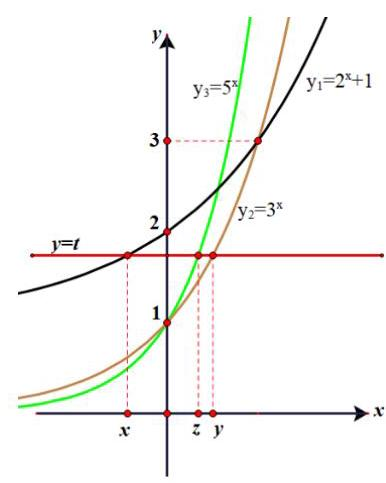
\includegraphics[max width=0.3\textwidth]{images/bo_d6dceus601uc73dvofhg_11_232_183_386_483_0.jpg}
\end{center}
\hspace*{3em} 

图 15-1

\begin{center}
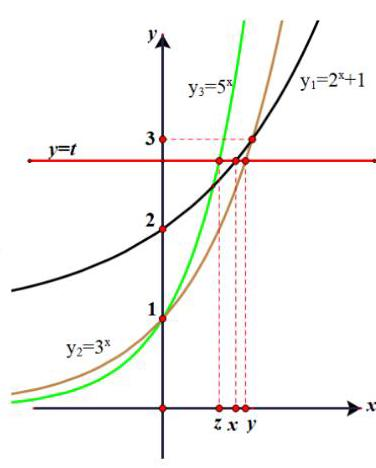
\includegraphics[max width=0.3\textwidth]{images/bo_d6dceus601uc73dvofhg_11_622_190_376_468_0.jpg}
\end{center}
\hspace*{3em} 

图 15-2

\begin{center}
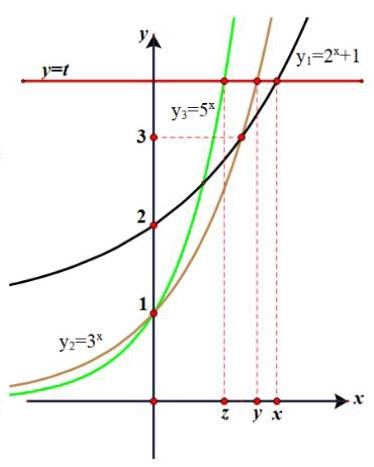
\includegraphics[max width=0.3\textwidth]{images/bo_d6dceus601uc73dvofhg_11_999_193_374_467_0.jpg}
\end{center}
\hspace*{3em} 

图 15-3

\section*{3.2 三要素}

1.【2025.12 黄浦高三一模 1】函数 \(y = \sqrt{x - 2}\) 的定义域是\_\_\_\_\_.

【答案】 \(\lbrack 2, + \infty )\)

【解析】定义域为 \(\lbrack 2, + \infty )\) .

2.【2025.12 虹口高三一模 2】函数 \(y = \sqrt{\frac{x + 1}{x - 2}}\) 的定义域为\_\_\_\_\_.

【答案】 \(( - \infty , - 1\rbrack  \cup  \left( {2, + \infty }\right)\)

【解析】依题意可得: \(\frac{x + 1}{x - 2} \geq  0\) ,解得 \(x \leq   - 1\) 或 \(x > 2\) , \(\therefore\) 定义域为 \(( - \infty , - 1\rbrack  \cup  \left( {2, + \infty }\right)\) .

3.【2025.12】浦东高三一模 2】函数 \(y = \lg \left( {x + 1}\right)\) 的定义域为\_\_\_\_\_.

【答案】定义域为 \(\left( {-1, + \infty }\right)\) .

4.【2025.12 金山高三一模 4】函数 \(y = \sqrt{{x}^{2} - {2x} - 3}\) 的定义域为\_\_\_\_\_.

【答案】 \(\left( {-\infty , - 1\rbrack \cup \lbrack 3, + \infty }\right)\)

【解析】解不等式: \({x}^{2} - {2x} - 3 \geq  0\) ,得 \(x \leq   - 1\) 或 \(x \geq  3\) , \(\therefore\) 定义域为 \(\left( {-\infty , - 1}\right\rbrack   \cup  \left\lbrack  {3, + \infty }\right)\) .

5.【2025.12 长宁高三一模 8】函数 \(y = \frac{1}{x - 1},x \in  D\) 的值域为 \(\left( {-1,0}\right)  \cup  \left( {0, + \infty }\right)\) ,则集合 \(D =\) \_\_\_\_\_.

【答案】由 \(y = \frac{1}{x - 1}\) 的函数图像可知: \(D = \left( {-\infty ,0}\right)  \cup  \left( {1, + \infty }\right)\) .

6.【2025.12 杨浦高三一模 16】函数 \(y = f\left( x\right)\) 的定义域、值域均为 \(R\) ,定义集合 \({M}_{a} = \{ t \mid  t = f\left( x\right)  - f\left( a\right) ,x \geq  a\}\) . 给出如下两个结论:  \circled{1} 存在函数 \(y = f\left( x\right)\) ,使得对任意实数 a 均有 \({M}_{a} = \lbrack 0, + \infty )\) ;

 \circled{2} 对任意函数 \(y = f\left( x\right)\) ，都存在实数 \(b\) ，使得对任意实数 \(a\) 均有 \({M}_{b} \subseteq  {M}_{a}\) . 下面判断正确的是( ).

A.  \circled{1} 正确， \circled{2} 正确 B.  \circled{1} 正确， \circled{2} 错误

C.  \circled{1} 错误， \circled{2} 正确 D.  \circled{1} 错误， \circled{2} 错误

【答案】B

【解析】对于命题 \circled{1} : 若 \(f\left( x\right)\) 在 \(\mathbb{R}\) 上单调递增,则 \(t = f\left( x\right)  - f\left( a\right)\) 在 \(x \in  \lbrack a, + \infty )\) 时也是单调递增,此时 \(t = f\left( x\right)  - f\left( a\right)  \in  \lbrack 0, + \infty )\) ,故 \circled{1} 为真命题;

(也可以直接举例: 如 \(f\left( x\right)  = x\) ,则 \(t = x - a\) 在 \(x \in  \lbrack a, + \infty )\) 时的值域也为 \(\lbrack 0, + \infty )\) )

对命题 \circled{2} : 取 \(f\left( x\right)  = \left\{  \begin{array}{ll} 0 & x = 0 \\  \frac{1}{x} & x \neq  0 \end{array}\right.\) .

若 \(b < 0,{M}_{b} = \{ t \mid  t = f\left( x\right)  - f\left( b\right) ,x \geq  b\}  = \left( {-\infty ,0\rbrack \cup \lbrack  - \frac{1}{b}, + \infty }\right)\) .

\(a = 2\) ,则 \({M}_{a} = \{ t \mid  t = f\left( x\right)  - f\left( a\right) ,x \geq  a\}  = \left( {-\frac{1}{2},0}\right\rbrack\) ,此时并不满足 \({M}_{b} \subseteq  {M}_{a}\) ;

若 \(b = 0\) ,则 \({M}_{b} = \{ t \mid  t = f\left( x\right)  - f\left( b\right) ,x \geq  b\}  = \{ t \mid  t = f\left( x\right) ,x \geq  0\}  = \lbrack 0, + \infty )\) .

此时取 \(a = 2\) ,则 \({M}_{a} = \left\{  {t\left| {\;t = f\left( x\right)  - \frac{1}{2}}\right. ,x \geq  2}\right\}   = \left( {-\frac{1}{2},0}\right\rbrack\) ,此时也并不满足 \({M}_{b} \subseteq  {M}_{a}\) ;

若 \(b > 0\) ,则 \({M}_{b} = \left\{  {t\left| {\;t = f\left( x\right)  - f\left( b\right) }\right. ,x \geq  b}\right\}   = \left\{  {t\left| {\;t = \frac{1}{x} - \frac{1}{b}}\right. ,x \geq  b}\right\}   = \left( {-\frac{1}{b},0}\right\rbrack\) .

取 \(a > b > 0\) ，则 \({M}_{a} = \left\{  {t \mid  t = f\left( x\right)  - f\left( a\right) ,x \geq  a}\right\}   = \left\{  {t\left| {\;t = \frac{1}{x} - \frac{1}{a}}\right. ,x \geq  a}\right\}   = \left( {-\frac{1}{a},0}\right\rbrack\) .

\(\because a > b > 0,\therefore 0 >  - \frac{1}{a} >  - \frac{1}{b}\) ,能时也不满足 \({M}_{b} \subseteq  {M}_{a}\) .

综上所述: 并不存在实数 \(b\) ,使得对任意的 \(a \in  \mathbb{R}\) 均有 \({M}_{b} \subseteq  {M}_{a}\) ,故  \circled{2} 为假命题. \(\propto\)

\section*{3.3 四性质}

1.【2025.12 宝山高三一模 7】已知 \(f\left( x\right)  = \ln \left( {2 + x}\right)  + \ln \left( {1 + {ax}}\right)\) 是偶函数，则函数 \(y = f\left( x\right)\) 的最大值为\_\_\_\_\_.

【答案】根据偶函数的定义域关于原点对称可知: \(a =  - \frac{1}{2}\) ,定义域为 \(\left( {-2,2}\right)\) .

此时 \(f\left( x\right)  = \ln \left( {2 + x}\right)  + \ln \left( {1 - \frac{x}{2}}\right)  = \ln \left( {2 + x}\right)  + \ln \left( {2 - x}\right)  - \ln 2 = \ln \left( {4 - {x}^{2}}\right)  - \ln 2\) .

易得: 当 \(x \in  \left( {-2,0}\right)\) 时, \(y = f\left( x\right)\) 单调递增; 当 \(x \in  \left( {0,2}\right)\) 时, \(y = f\left( x\right)\) 单调递减.

所以 \(y = f\left( x\right)\) 的最大值为 \(f\left( 0\right)  = \ln 2. \ll\)

2.【2025.12 奉贤高三一模 8】若函数 \(y = \frac{a \cdot  {2}^{x} - 1}{{2}^{x} + 1}\left( {a \in  \mathbf{R}}\right)\) 是偶函数,则实数 \(a =\) \_\_\_\_\_.

【答案】 \(a =  - 1\)

【解析】依题意可得: 函数的定义域为 \(\mathbb{R}\) ,

\(\therefore f\left( 1\right)  = f\left( {-1}\right)\) ,即 \(\frac{{2a} - 1}{3} = \frac{\frac{a}{2} - 1}{\frac{3}{2}}\) ,解得 \(a =  - 1\) .

3.【2025.12 崇明高三一模 9】已知 \(y = f\left( x\right)\) 是定义在 \(\mathbf{R}\) 上的奇函数,且当 \(x > 0\) 时, \(f\left( x\right)  = {x}^{2} - {3}^{x}\) ,则 \(f\left( {-1}\right)  =\) \_\_\_\_\_.

【答案】 2

【解析】依题意可得: \(f\left( {-1}\right)  =  - f\left( 1\right)  = 2\)

4. 【2025.12 杨浦高三一模 10】已知定义在 \(R\) 上的函数 \(y = f\left( x\right)\) 为奇函数,且 \(g\left( x\right)  = \left\{  \begin{matrix} {2}^{x} & x \geq  0 \\  f\left( x\right) & x < 0 \end{matrix}\right.\) 为偶函数，则 \(f\left( {{\log }_{2}3}\right)  =\) \_\_\_\_\_.

答案: -3

【解析】依题意可得 \(f\left( {{\log }_{2}3}\right)  =  - f\left( {-{\log }_{2}3}\right)  =  - g\left( {-{\log }_{2}3}\right)  =  - g\left( {{\log }_{2}3}\right)  =  - 3\) .

5.【2025.12 虹口高三一模 11】若 \(\left\{  {x\left| {\;\lg \left( {{x}^{2} + {2x}}\right)  - \lg \left( {a \cdot  {\mathrm{e}}^{x} - 1}\right)  = 0}\right. }\right\}   \neq  \varnothing\) ,则实数 \(a\) 的取值范围是\_\_\_\_\_.

【答案】 \(\left( {0,\frac{4}{e}}\right\rbrack   \cup  \left( {{e}^{2}, + \infty }\right)\)

【解析】原题等价于 “ \({x}^{2} + {2x} = a \cdot  {e}^{x} - 1 > 0\) ”,也等价于 “方程 \({x}^{2} + {2x} = a \cdot  {e}^{x} - 1\) 在

\(\left( {-\infty , - 2}\right)  \cup  \left( {0, + \infty }\right)\) 上有解”. 参变分离得: \(a = \frac{{x}^{2} + {2x} + 1}{{e}^{x}}\) ,

设 \(g\left( x\right)  = \frac{{x}^{2} + {2x} + 1}{{e}^{x}}\) ,其中 \(\left( {-\infty , - 2}\right)  \cup  \left( {0, + \infty }\right)\) .

易得 \({g}^{\prime }\left( x\right)  = \frac{\left( {{2x} + 2}\right) {e}^{x} - {e}^{x}\left( {{x}^{2} + {2x} + 1}\right) }{{\left( {e}^{x}\right) }^{2}} = \frac{1 - {x}^{2}}{{e}^{x}}\) . 令 \({g}^{\prime }\left( x\right)  = 0\) 得 \(x = 1\left( {x =  - 1\text{ 舍 }}\right)\) .

所以当 \(x \in  \left( {-\infty , - 2}\right)\) 时, \({g}^{\prime }\left( x\right)  < 0,g\left( x\right)  = \frac{{x}^{2} + {2x} + 1}{{e}^{x}}\) 单调递减;

且 \(g\left( {-2}\right)  = \frac{1}{{e}^{-2}} = {e}^{2}\) ,当 \(x \rightarrow   - \infty\) 时, \(g\left( x\right)  \rightarrow   + \infty\) ; 此时 \(y = g\left( x\right)\) 的值域为 \(\left( {{e}^{2}, + \infty }\right)\) ;

\(x \in  \left( {0,1}\right)\) 时, \({g}^{\prime }\left( x\right)  > 0,g\left( x\right)  = \frac{{x}^{2} + {2x} + 1}{{e}^{x}}\) 单调递增;

\(x \in  \left( {1, + \infty }\right)\) 时, \({g}^{\prime }\left( x\right)  < 0,g\left( x\right)  = \frac{{x}^{2} + {2x} + 1}{{e}^{x}}\) 单调递减;

极大值为 \(g\left( 1\right)  = \frac{4}{e}\) ,且 \(x \rightarrow  0\) 时, \(g\left( x\right)  \rightarrow  1\) ,当 \(x \rightarrow   + \infty\) 时, \(g\left( x\right)  \rightarrow  0\) ; 此时 \(y = g\left( x\right)\) 的值域为 \(\left( {0,\frac{4}{e}}\right\rbrack\) .

综上所述: \(y = g\left( x\right)\) 的值域为 \(\left( {0,\frac{4}{e}}\right\rbrack   \cup  \left( {{e}^{2}, + \infty }\right)\) ,

即实数 \(a\) 的取值范围是 \(\left( {0,\frac{4}{e}}\right\rbrack   \cup  \left( {{e}^{2}, + \infty }\right)\) .

6.【2025.12 嘉定高三一模 11】已知 \(f\left( x\right)  = \ln \frac{1 - {x}^{3}}{1 + {x}^{3}}\) ,且 \(f\left( {1 - a}\right)  + f\left( {1 - {a}^{2}}\right)  > 0\) ,则实数 \(a\) 的取值范围是\_\_\_\_\_.

【答案】 \(\left( {1,\sqrt{2}}\right)\)

【解析】不难发现: \(f\left( x\right)  = \ln \frac{1 - {x}^{3}}{1 + {x}^{3}}\) 是定义在 \(\left( {-1,1}\right)\) 上的奇函数,且严格递减.

\(\therefore\) 由 \(f\left( {1 - a}\right)  + f\left( {1 - {a}^{2}}\right)  > 0\) 得 \(f\left( {1 - a}\right)  >  - f\left( {1 - {a}^{2}}\right)  = f\left( {{a}^{2} - 1}\right)\) ,

\(\therefore \left\{  \begin{array}{l}  - 1 < 1 - a < 1 \\   - 1 < 1 - {a}^{2} < 1 \Rightarrow  1 < a < \sqrt{2} \\  1 - a < {a}^{2} - 1 \end{array}\right.\) .

7.【2025.12 黄浦高三一模 13】下列函数中,既是偶函数又在 \(\left\lbrack  {0,1}\right\rbrack\) 上严格减的函数是 ( )

A. \(y =  - x\) B. \(y =  - \left| x\right|\) C. \(y = {x}^{2}\) D. \(y = {2}^{-x}\)

【答案】B\$

8.【2025.12 奉贤高三一模 13】设 \(a\text{ 、 }b\) 为实数，且 \(a > b > 0\) ，则下列不等式一定正确的是 ( )

A. \({a}^{4} > {b}^{2}\) B. \(\sin a > \sin b\)

C. \(c > 0\) 时, \({\left( \frac{b}{a}\right) }^{c} > 1\;\) D. \(\ln a > \ln b\)

【答案】D

【解析】由 \(y = \ln x\) 的单调性可知 \(\mathrm{D}\) 正确. \(>  <\)

9.【2025.12 松江高三一模 14】下列函数 \(y = f\left( x\right)\) 中,对任意的 \({x}_{1},{x}_{2} \in  \left( {0, + \infty }\right)\) 时,均有 \(\left( {{x}_{1} - {x}_{2}}\right) \left\lbrack  {f\left( {x}_{1}\right)  - f\left( {x}_{2}\right) }\right\rbrack   > 0\) 的是( )

A. \(f\left( x\right)  = {x}^{-2}\) B. \(f\left( x\right)  = {x}^{2} - {4x} + 4\) C. \(f\left( x\right)  = {2}^{x}\) D. \(f\left( x\right)  = {\log }_{\frac{1}{2}}x\)

【答案】C

【解析】四个选项中,只有 \(\mathrm{C}\) 中的 \(f\left( x\right)  = {2}^{x}\) 在 \(\left( {0, + \infty }\right)\) 上单调递增,故选 C. \(>\)

10.【2025.12 闵行高三一模 16】如果“若 \(p\) ,则 \(q\) ”和“若 \(q\) ,则 \(p\) ”中有且仅有一个真命题, 称 \(p\) 与 \(q\) 具有“ \(U\) -关系”. 已知函数 \(y = f\left( x\right)\) 的定义域为 \(\mathbf{R},p : y = f\left( x\right)\) 为偶函数,则 \(p\) 与下列选项中的 \(q\) 具有“ \(U\) -关系”的为( ).

A. \(q\) : 对任意 \(x \in  \mathbf{R}\) 都有 \(- f\left( x\right)  \geq  f\left( x\right)\) B. \(q\) : 对任意 \(x \in  \mathbf{R}\) 都有 \(f\left( {-x}\right)  \geq  f\left( x\right)\)

C. \(q :\) 对任意 \(x \in  \mathbf{R}\) 都有 \(f\left( {-x}\right)  = \left| {f\left( x\right) }\right|\) D. \(q\) : 对任意 \(x \in  \mathbf{R}\) 都有 \(f\left( {-x}\right)  = f\left( \left| x\right| \right)\)

【答案】C

【解析】A 选项等价于“恒有 \(f\left( x\right)  \leq  0\) ”,与 \(y = f\left( x\right)\) 为偶函数并无关系, A 错误;

B 选项: 若 \(y = f\left( x\right)\) 为偶函数,则 \(f\left( {-x}\right)  = f\left( x\right)\) ,此时 \(f\left( {-x}\right)  \geq  f\left( x\right)\) 成立;

反之,若对任意的 \(x \in  \mathbb{R}\) 恒有 \(f\left( {-x}\right)  \geq  f\left( x\right)\) 成立,则当每个 \(x\) 都取 \(- x\) 时,有

\(f\left( x\right)  \geq  f\left( {-x}\right)\) ,因此只能是 \(f\left( {-x}\right)  = f\left( x\right)\) ,即 \(y = f\left( x\right)\) 为偶函数,所以 \(\mathrm{B}\) 选项互为充要条件;

C 选项: 若 \(y = f\left( x\right)\) 为偶函数,则 \(f\left( {-x}\right)  = f\left( x\right)\) ,但 \(f\left( {-x}\right)  = \left| {f\left( x\right) }\right|\) 不一定成立,如 \(f\left( x\right)  = \cos x\)

反之,若对任意的 \(x \in  \mathbb{R}\) 恒有 \(f\left( {-x}\right)  = \left| {f\left( x\right) }\right|\) 成立,则当每个 \(x\) 都取 \(- x\) 时,有

\(f\left( x\right)  = \left| {f\left( {-x}\right) }\right|  = \left| {f\left( x\right) }\right|  = f\left( {-x}\right)\) ,即 \(y = f\left( x\right)\) 为偶函数成立,所以 \(\mathrm{C}\) 正确;

D 选项: 若 \(y = f\left( x\right)\) 为偶函数,则 \(f\left( {-x}\right)  = f\left( x\right)\) .

若 \(x \geq  0\) ,则 \(f\left( {-x}\right)  = f\left( x\right)  = f\left( \left| x\right| \right)\) 成立;

若 \(x < 0\) ,则 \(f\left( x\right)  = f\left( {-x}\right)  = f\left( \left| x\right| \right)\) ,每个 \(x\) 都取 \(- x\) 时, \(f\left( {-x}\right)  = f\left( \left| {-x}\right| \right)  = f\left( \left| x\right| \right)\) 成立;

综上所述: \(x \in  \mathbb{R}\) 时,若 \(y = f\left( x\right)\) 为偶函数,则均有 \(f\left( {-x}\right)  = f\left( \left| x\right| \right)\) 成立;

反之,若对任意的 \(x \in  \mathbb{R}\) 恒有 \(f\left( {-x}\right)  = f\left( \left| x\right| \right)\) 成立,则当 \(x \geq  0\) 时,则 \(f\left( {-x}\right)  = f\left( \left| x\right| \right)  = f\left( x\right)\) 成立;

若 \(x < 0\) ,则由 \(f\left( {-x}\right)  = f\left( \left| x\right| \right)\) 得: 每个 \(x\) 都取 \(- x\) 时,有 \(f\left( x\right)  = f\left( \left| {-x}\right| \right)  = f\left( \left| x\right| \right)  = f\left( {-x}\right)\) , 即 \(y = f\left( x\right)\) 为偶函数，所以 D 选项互为充要条件.

\section*{3.4 方程与不等式}

1.【2025.12 青浦高三一模 11】已知函数 \(f\left( x\right)  = {\mathrm{e}}^{x - 1} - {ax} + a\left( {a > 0}\right)\) ,若 \(f\left( x\right)  < 0\) 仅存在唯一整数解,则实数 \(a\) 的取值范围是\_\_\_\_\_.

【答案】 \(\left( {\mathrm{e},\frac{{\mathrm{e}}^{2}}{2}}\right\rbrack\) .

【解析】依题意可得: 不等式 \({e}^{x - 1} - {ax} + a < 0\) 有唯一整数解,即 \({e}^{x - 1} < a\left( {x - 1}\right)\) 有唯一整数解. 也等价于 \({e}^{x} < {ax}\) 有唯一整数解,分别设 \(f\left( x\right)  = {e}^{x},g\left( x\right)  = {ax}\) .

先画图,找出二者相切的情况: 当 \(g\left( x\right)  = {ax}\) 与 \(f\left( x\right)  = {e}^{x}\) 相切时,切点为 \(\left( {1,e}\right)\) ,此时 \(a = e\) . 根据“不等式 \({e}^{x} < {ax}\) 有唯一整数解”得 \(\left\{  \begin{array}{l} f\left( 1\right)  < g\left( 1\right) \\  f\left( 2\right)  \geq  g\left( 2\right)  \end{array}\right.\) ,解得 \(\frac{{e}^{2}}{2} \geq  a > e\) .

\section*{3.5 方程根与零点问题}

1.【2025.12 青浦高三一模 7】若函数 \(y = \left| {{2}^{x} - 1}\right|\) 的图像与直线 \(y = b\) 有两个公共点,则实数 \(b\) 的取值范围是\_\_\_\_\_.

【答案】 \(\left( {0,1}\right)\)

【解析】画出 \(y = \left| {{2}^{x} - 1}\right|\) 的图像,由图可知: \(b \in  \left( {0,1}\right)\) .

\begin{center}
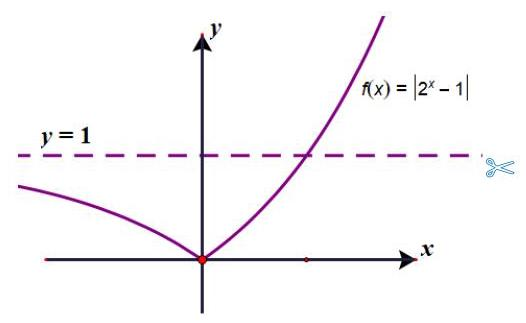
\includegraphics[max width=0.4\textwidth]{images/bo_d6dceus601uc73dvofhg_16_888_1685_526_323_0.jpg}
\end{center}
\hspace*{3em} 

2.【2025.12 徐汇高三一模 10】设 \(f\left( x\right)  = \left\{  \begin{array}{ll} \left| {x - 2}\right| & x \geq  0 \\   - \frac{1}{x} & x < 0 \end{array}\right.\) ,若实数 \({x}_{1},{x}_{2},{x}_{3}\) 满足 \({x}_{1} < {x}_{2} < {x}_{3}\) 且 \(f\left( {x}_{1}\right)  = f\left( {x}_{2}\right)  = f\left( {x}_{3}\right)\) ，则 \(\frac{\sqrt{{x}_{2}{x}_{3}}}{{x}_{1}}\) 的最小值为\_\_\_\_\_.

【答案】 -2

【解析】设 \(f\left( {x}_{1}\right)  = f\left( {x}_{2}\right)  = f\left( {x}_{3}\right)  = t\) ,则根据图像可知: \(t \in  (0,2\rbrack ,\therefore \left\{  \begin{array}{l} {x}_{1} =  - \frac{1}{t} \\  {x}_{2} = 2 - t \\  {x}_{1} = 2 + t \end{array}\right.\) , \(\therefore \frac{\sqrt{{x}_{2}{x}_{3}}}{{x}_{1}} =  - t \cdot  \sqrt{4 - {t}^{2}} =  - \sqrt{4{t}^{2} - {t}^{4}} =  - \sqrt{-{\left( {t}^{2} - 2\right) }^{2} + 4} \geq   - 2\) ,当且仅当 \({t}^{2} = 2\) 即 \(t = \sqrt{2}\) 时等号成立.

3.【2025.12 静安高三一模 12】设 \(y = f\left( x\right)\) 是定义在 \(\mathbb{R}\) 上的偶函数,对任意的 \(x \in  \mathbb{R}\) ,都有 \(f\left( {-x}\right)  = f\left( {x + 4}\right)\) ,且当 \(x \in  \left\lbrack  {-2,0}\right\rbrack\) 时, \(f\left( x\right)  = {\left( \frac{1}{2}\right) }^{x} - 1\) . 设 \(g\left( x\right)  = f\left( x\right)  - {\log }_{a}\left( {x + 2}\right)\) (其中 \(a > 1)\) ,若函数 \(y = g\left( x\right)\) 在左开右闭区间 \(( - 2,6\rbrack\) 上恰有 3 个不同的零点,则实数 \(a\) 的取值范围是\_\_\_\_\_.

【答案】 \(\left( {\sqrt[3]{4},2}\right)\)

【解析】由 \(f\left( {-x}\right)  = f\left( {x + 4}\right)\) 可得 \(y = f\left( x\right)\) 关于 \(x = 2\) 轴对称,同时, \(y = f\left( x\right)\) 是偶函数,可得 \(y = f\left( x\right)\) 为周期函数,最小正周期为 4 .

当 \(x \in  \left\lbrack  {0,2}\right\rbrack\) 时, \(- x \in  \left\lbrack  {-2,0}\right\rbrack  ,\therefore f\left( x\right)  = f\left( {-x}\right)  = {\left( \frac{1}{2}\right) }^{-x} - 1 = {2}^{x} - 1\) 。

从而再由最小正周期为 4 可以画出 (-2,6] 上的函数图像.

当 \(g\left( x\right)  = f\left( x\right)  - {\log }_{a}\left( {x + 2}\right)\) 在 \(( - 2,6\rbrack\) 上有 3 个零点,等价于 \(y = f\left( x\right)\) 与 \(y = {\log }_{a}\left( {x + 2}\right)\) 在 \(( - 2,6\rbrack\) 上有 3 个交点,则画出图像,找出临界情况,如图所示: 分别为 \(y = {\log }_{a}\left( {x + 2}\right)\) 过 \(A\left( {2,3}\right)\) 和 \(B\left( {6,3}\right)\) ,代入计算得 \(a = \sqrt[3]{4}\) 和 \(a = 3\) ,所以符合题意的 \(a \in  \left( {\sqrt[3]{4},2}\right)\) .

\begin{center}
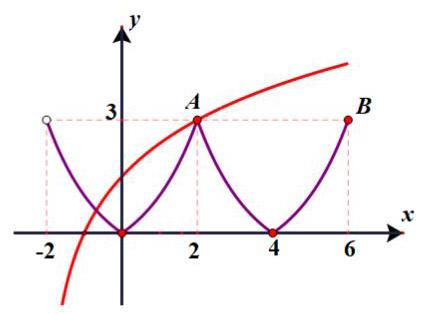
\includegraphics[max width=0.3\textwidth]{images/bo_d6dceus601uc73dvofhg_18_440_199_422_314_0.jpg}
\end{center}
\hspace*{3em} 

\begin{center}
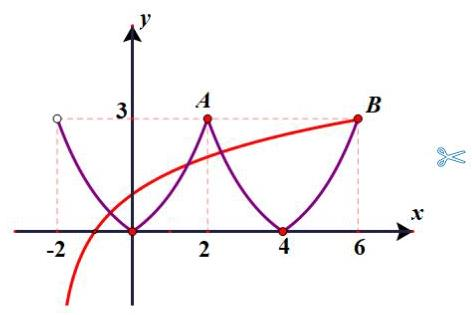
\includegraphics[max width=0.4\textwidth]{images/bo_d6dceus601uc73dvofhg_18_937_199_472_315_0.jpg}
\end{center}
\hspace*{3em} 

4.【2025.12 松江高三一模 15】已知函数 \(f\left( x\right)  = 6{\left( x - 2k\right) }^{2},x \in  \left\lbrack  {{2k} - 1,{2k} + 1}\right\rbrack  \left( {k \in  \mathbb{Z}}\right)\) ,函数 \(g\left( x\right)  = a{x}^{2} + x + c\) . 若对任意 \({x}_{1},{x}_{2} \in  \mathbb{R}\) ,都有 \(g\left( {{x}_{1} + {x}_{2}}\right)  = g\left( {x}_{1}\right)  + g\left( {x}_{2}\right)  + 4\) ,则方程 \(f\left( x\right)  = g\left( x\right)\) 的解的个数为( )

A. 6 B. 7 C. 8 D. 9

【答案】B

【解析】: 对任意 \({x}_{1},{x}_{2} \in  \mathbb{R},g\left( {{x}_{1} + {x}_{2}}\right)  = g\left( {x}_{1}\right)  + g\left( {x}_{2}\right)  + 4\) 恒成立,代入化简得 \({2a}{x}_{1}{x}_{2} = c + 4\) 恒成立, \(\therefore a = 0\) 且 \(c =  - 4\) ,此时 \(g\left( x\right)  = x - 4\) .

再画出 \(f\left( x\right)  = 6{\left( x - 2k\right) }^{2},x \in  \left\lbrack  {{2k} - 1,{2k} + 1}\right\rbrack  \left( {k \in  \mathbb{Z}}\right)\) 的图像,如下图:

\begin{center}
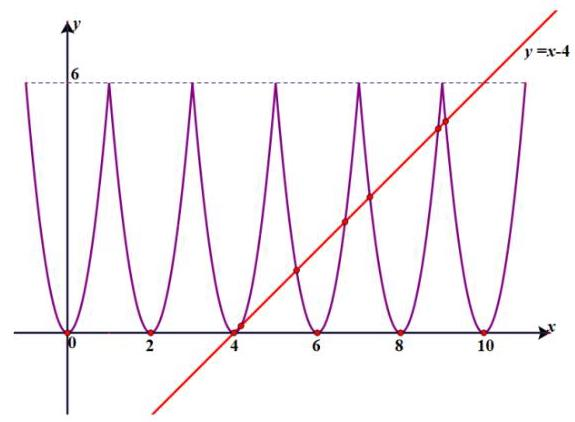
\includegraphics[max width=0.4\textwidth]{images/bo_d6dceus601uc73dvofhg_18_819_1044_575_422_0.jpg}
\end{center}
\hspace*{3em} 

由图可知: \(y = f\left( x\right)\) 与直线 \(g\left( x\right)  = x - 4\) 的交点个数为 7,选 B.C.

5.【2025.12 静安高三一模 16】已知函数 \(f\left( x\right)  = \ln \left( {x + 1}\right)  + \frac{ax}{x + 1}\left( {a \in  \mathbb{R}}\right)\) . 现有下述两个结论，下列说法正确的是( ).

 \circled{1}  若 \(y = f\left( x\right)\) 在区间 \(\left( {-1,0}\right)\) 内恰有一个零点，则 \(a\) 的取值范围是 \(\left( {-1,0}\right)\) ；

 \circled{2}  若 \(a > 0\) ，则方程 \({f}^{\prime }\left( x\right)  - f\left( x\right)  = \frac{\sqrt{5} - 1}{2} - \ln \frac{\sqrt{5} + 1}{2}\) 的解为 \(x = \frac{-1 \pm  \sqrt{5}}{2}\) .

A. 结论 \circled{1} 和 \circled{2} 均正确 B. 结论 \circled{1} 正确，结论 \circled{2} 错误

C. 结论 \circled{1} 错误，结论 \circled{2} 正确 D. 结论 \circled{1} 和 \circled{2} 均错误

【答案】B

【解析】对命题 \circled{1} : 令 \(f\left( x\right)  = 0\) 得 \(- {ax} = \left( {x + 1}\right) \ln \left( {x + 1}\right)\) .

再设 \(g\left( x\right)  = \left( {x + 1}\right) \ln \left( {x + 1}\right)\) ,其中 \(x \in  \left( {-1,0}\right)\) ,则 \({g}^{\prime }\left( x\right)  = \ln \left( {x + 1}\right)  + 1\) .

从而可知: \(g\left( x\right)  = \left( {x + 1}\right) \ln \left( {x + 1}\right)\) 在 \(\left( {-1,\frac{1}{e} - 1}\right)\) 上单调递减,在 \(\left( {\frac{1}{e} - 1,0}\right)\) 上单调递增.

画出 \(g\left( x\right)  = \left( {x + 1}\right) \ln \left( {x + 1}\right)\) 的图像.

\begin{center}
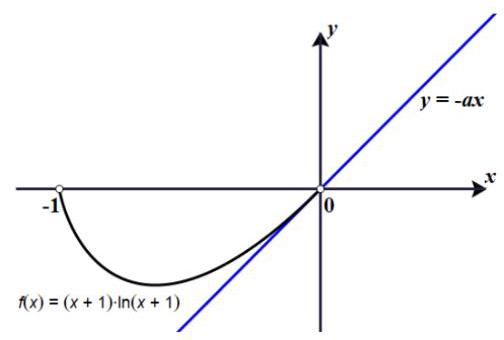
\includegraphics[max width=0.4\textwidth]{images/bo_d6dceus601uc73dvofhg_19_896_425_504_340_0.jpg}
\end{center}
\hspace*{3em} 

当 \(y = f\left( x\right)\) 在区间 \(\left( {-1,0}\right)\) 内恰有一个零点,等价于直线 \(y =  - {ax}\) 与 \(g\left( x\right)  = \left( {x + 1}\right) \ln \left( {x + 1}\right)\) 在区间 \(\left( {-1,0}\right)\) 内恰有一个交点. 找出临界情况: 即直线 \(y =  - {ax}\) 与 \(g\left( x\right)  = \left( {x + 1}\right) \ln \left( {x + 1}\right)\) 在 \(x = 0\) 处相切.

易得 \({g}^{\prime }\left( x\right)  = 1 + \ln \left( {x + 1}\right) ,\therefore {g}^{\prime }\left( 0\right)  = 1\) ,故 \(1 >  - a > 0\) ,即满足条件的 \(a\) 的取值范围是 \(\left( {-1,0}\right)\) , \circled{1} 为真命题;

对命题 \circled{2} :由 \(f\left( x\right)  = \ln \left( {x + 1}\right)  + \frac{ax}{x + 1}\) 得定义域为 \(x \in  \left( {-1, + \infty }\right)\) ，且 \({f}^{\prime }\left( x\right)  = \frac{1}{x + 1} + \frac{a}{{\left( x + 1\right) }^{2}}\) . 设 \(g\left( x\right)  = {f}^{\prime }\left( x\right)  - f\left( x\right)  = \frac{1}{x + 1} + \frac{a}{{\left( x + 1\right) }^{2}} - \ln \left( {x + 1}\right)  - \frac{ax}{x + 1} = \frac{1 + a}{x + 1} + \frac{a}{{\left( x + 1\right) }^{2}} - \ln \left( {x + 1}\right)  - a.\)

所以 \({g}^{\prime }\left( x\right)  =  - \frac{1 + a}{{\left( x + 1\right) }^{2}} - \frac{2a}{{\left( x + 1\right) }^{3}} - \frac{1}{x + 1} < 0\) ,即 \(g\left( x\right)  = {f}^{\prime }\left( x\right)  - f\left( x\right)\) 在 \(\left( {-1, + \infty }\right)\) 上单调递减, \(\therefore {f}^{\prime }\left( x\right)  - f\left( x\right)  = \frac{\sqrt{5} - 1}{2} - \ln \frac{\sqrt{5} + 1}{2}\) 不可能有个根 \(x = \frac{-1 \pm  \sqrt{5}}{2}\) ,即 \circled{2} 为假命题. \(>\)

6.【2025.12 浦东高三一模 16】已知函数 \(y = f\left( x\right)\) ，其中 \(f\left( x\right)  = x - \frac{1}{x},x > 0\) . 集合 \(A = \{ 1,a,b\}\) ， 其中 \(1 < a < b\) ,集合 \(B = \left\{  {z\left| {\;z = {xy} + \frac{x}{y} + f\left( \frac{y}{x}\right) }\right. ,x,y \in  A,x \neq  y}\right\}\) ,现有以下两个命题:  \circled{1} 存在实数 \(a\text{ 、 }b\) ,使得集合 \(B\) 中恰好有 5 个元素;

 \circled{2}  若实数 \(a\text{ 、 }b\) 是方程 \(f\left( x\right)  = {kx} + t\) 的两个不同实根，则存在实数 \(k\text{ 、 }t\) ，使得集合 \(B\) 中恰好有 4 个元素. 那么( )

A.  \circled{1} 是真命题， \circled{2} 是真命题 B.  \circled{1} 是假命题， \circled{2} 是假命题

C.  \circled{1} 是真命题， \circled{2} 是假命题 D.  \circled{1} 是假命题， \circled{2} 是真命题

【答案】A

【解析】先化简: \(z = {xy} + \frac{x}{y} + f\left( \frac{y}{x}\right)  = {xy} + \frac{x}{y} + \frac{y}{x} - \frac{x}{y} = {xy} + \frac{y}{x}\) ,

得集合 \(B = \left\{  {z\left| {\;z = {xy} + \frac{y}{x}}\right. ,x,y \in  \{ 1,x,y\} ,x \neq  y}\right\}\) .

当 \(x = 1\) ， \(y = a\) 时， \(z = {2a}\) ；当 \(x = a\) ， \(y = 1\) 时， \(z = a + \frac{1}{a}\) ；当 \(x = 1\) ， \(y = b\) 时， \(z = {2b}\) ； 当 \(x = b\) ， \(y = 1\) 时， \(z = b + \frac{1}{b}\) ；当 \(x = a\) ， \(y = b\) 时， \(z = {ab} + \frac{b}{a}\) ；当 \(x = b\) ， \(y = a\) 时， \(z = {ab} + \frac{a}{b}\)

\(\because 1 < a < b,\therefore \left\{  \begin{array}{l} {ab} + \frac{b}{a} > {2b} > b + \frac{1}{b} \\  {ab} + \frac{a}{b} > {2a} > a + \frac{1}{a} \end{array}\right.\) ; 且同时 \(\left\{  \begin{array}{l} {ab} + \frac{b}{a} > {ab} + \frac{a}{b} \\  {2b} > {2a} \\  b + \frac{1}{b} > a + \frac{1}{a} \end{array}\right.\) .

对命题 \circled{1} :当 \({2a} = b + \frac{1}{b}\) 时，可以取 \(a = \frac{5}{3},b = 3\) ，则此时集合 \(B = \left\{  {\frac{34}{5},\frac{50}{9},6,\frac{10}{3},\frac{34}{15}}\right\}\) ，恰好有 5 个元素, \(\therefore\)  \circled{1} 命题为真命题；

对命题 \circled{2} :当满足 \(\left\{  \begin{array}{l} {2a} = b + \frac{1}{b} \\  {ab} + \frac{a}{b} = {2b} \end{array}\right.\) 时，解得 \(b = {a}^{2}\) ，将其回代到第一个式子中得 \({a}^{4} - 2{a}^{3} + 1 = 0\)

设 \(f\left( x\right)  = {x}^{4} - 2{x}^{3} + 1\) ,易得 \({f}^{\prime }\left( x\right)  = 4{x}^{3} - 6{x}^{2} = 2{x}^{2}\left( {{2x} - 3}\right)\) ,

令 \({f}^{\prime }\left( x\right)  = 0\) 得 \(x = \frac{3}{2}\left( {x = 0\text{ 舍 }}\right)\) . 当 \(x \in  \left( {1,\frac{3}{2}}\right)\) 时, \({f}^{\prime }\left( x\right)  < 0,y = f\left( x\right)\) 单调递减;

当 \(x \in  \left( {\frac{3}{2}, + \infty }\right)\) 时, \({f}^{\prime }\left( x\right)  > 0,y = f\left( x\right)\) 单调递增; \(\therefore f{\left( x\right) }_{\text{ 极小值 }} = f\left( \frac{3}{2}\right)  =  - \frac{11}{16} < 0\) .

又 \(f\left( 1\right)  = 0,f\left( 2\right)  = 1 > 0\) ,由零点存在定理可得 \(y = f\left( x\right)\) 在 \(\left( {\frac{3}{2},2}\right)\) 必定存在一个零点 \(a \in  \left( {\frac{3}{2},2}\right)\) ,则 \(b = {a}^{2} > a > 1\) ,满足题意,此时 \(B\) 集合中刚好有 4 个元素,故 \circled{2} 也为真命

题.

7.【2025.12 嘉定高三一模 19】已知 \(f\left( x\right)  = {x}^{3} + {ax} + 1\) .

(1)若 \(a =  - 3\) ，求函数 \(y = f\left( x\right)\) 的单调区间.

(2)若 \(y = f\left( x\right)\) 在 \(\left( {0, + \infty }\right)\) 上存在零点，求实数 \(a\) 的最大值

【答案】(1)在 \(\left( {-\infty , - 1}\right)\) 、 \(\left( {1, + \infty }\right)\) 严格增，在 \(\left( {-1,1}\right)\) 严格减 (2) \(- \frac{3\sqrt[3]{2}}{2}\)

【解析】(1) \({f}^{\prime }\left( x\right)  = 3{x}^{2} - 3\) . 令 \({f}^{\prime }\left( x\right)  = 0\) ,解得 \(x =  \pm  1\) .

将不同驻点及其所划分出的区间列表如下:

\begin{center}
\adjustbox{max width=\textwidth}{
\begin{tabular}{|c|c|c|c|c|c|}
\hline
\(x\) & \(\left( {-\infty , - 1}\right)\) & -1 & (-1,1) & 1 & (1,+∞) \\
\cline{1-6}
\({f}^{\prime }\left( x\right)\) & + & 0 & - & 0 & + \\
\cline{1-6}
\(f\left( x\right)\) & ▼ & 极大值 & 一 & 极小值 & ▼ \\
\cline{1-6}
\hline
\end{tabular}
}
\end{center}

因此 \(y = f\left( x\right)\) 的单调增区间是 \(\left( {-\infty , - 1}\right)\) 及 \(\left( {1, + \infty }\right)\) ,单调减区间是 \(\left( {-1,1}\right)\) .

(2)由 \(f\left( x\right)  = 0\) 得 \({x}^{3} + {ax} + 1 = 0\left( {x > 0}\right) ,\;a =  - \frac{{x}^{3} + 1}{x} =  - {x}^{2} - \frac{1}{x}\) .

令 \(g\left( x\right)  =  - {x}^{2} - \frac{1}{x}\) ,则 “ \(y = f\left( x\right)\) 在 \(\left( {0, + \infty }\right)\) 上存在零点”等价于 “ \(a\) 是 \(y = g\left( x\right) ,x \in  \left( {0, + \infty }\right)\) 的某个函数值”. \({g}^{\prime }\left( x\right)  =  - {2x} + \frac{1}{{x}^{2}} = \frac{1 - 2{x}^{3}}{{x}^{2}}\) . 解 \({g}^{\prime }\left( x\right)  = 0\) ,得 \(x = \frac{\sqrt[3]{4}}{2}\) .

当 \(0 < x < \frac{\sqrt[3]{4}}{2}\) 时, \({g}^{\prime }\left( x\right)  > 0\) ,即 \(y = g\left( x\right)\) 在 \(\left( {0,\frac{\sqrt[3]{4}}{2}}\right)\) 内严格增. 当 \(x > \frac{\sqrt[3]{4}}{2}\) 时, \({g}^{\prime }\left( x\right)  < 0\) ,即

\(y = g\left( x\right)\) 在 \(\left( {\frac{\sqrt[3]{4}}{2}, + \infty }\right)\) 内严格减. 因此 \(y = g\left( x\right) ,x \in  \left( {0, + \infty }\right)\) 的最大值是 \(g\left( \frac{\sqrt[3]{4}}{2}\right)  =  - \frac{3\sqrt[3]{2}}{2}\) .

因此, \(a\) 的最大值是 \(- \frac{3\sqrt[3]{2}}{2}\) . \(\asymp\)

8.【2025.12 虹口高三一模 21】已知函数 \(y = f\left( x\right)\) 的定义域为 \(D\left( {D \subseteq  \mathbf{R}}\right)\) ,记 \(g\left( x\right)  = f\left( {x + a}\right)  - f\left( x\right)\) ,其中 \(a \in  D\) ,且 \(x + a \in  D.\)

(1)当 \(D = \mathbf{R},f\left( x\right)  = {x}^{2},a = 1\) ，求函数 \(y = g\left( x\right)\) 的零点:

( 2 )当 \(D = \lbrack  - 1, + \infty ),f\left( x\right)  = {x}^{3} - {3x}\) ，若恒有 \(g\left( x\right)  > 0\) ，求实数 \(a\) 的取值范围；

(3)当 \(D = \mathbf{Q}\) ,求证: “对于任意的正有理数 \(a\) ,函数 \(y = g\left( x\right)\) 在 \(D\) 上均是严格增函数”的充要条件是 “任取 \(D\) 中两个不相同的元素 \({x}_{1}\) 和 \({x}_{2}\) ,均有 \(f\left( \frac{{x}_{1} + {x}_{2}}{2}\right)  < \frac{1}{2}\left( {f\left( {x}_{1}\right)  + f\left( {x}_{2}\right) }\right)\) ”.

【答案】(1) \(x =  - \frac{1}{2}\) (2) \(a \in  \left( {3, + \infty }\right)\) (3)证明见解析

【解析】(1) \(g\left( x\right)  = {\left( x + 1\right) }^{2} - {x}^{2} = {2x} + 1,2\) 分

令 \(g\left( x\right)  = 0\) ,解得 \(x =  - \frac{1}{2}\) ,所以函数 \(y = g\left( x\right)\) 的零点为 \(x =  - \frac{1}{2}\) . 4 分

(2)解一: \({f}^{\prime }\left( x\right)  = 3{x}^{2} - 3\) ,所以当 \(x \in  \left( {-1,1}\right) ,{f}^{\prime }\left( x\right)  < 0,y = f\left( x\right)\) 为严格减函数,

当 \(x \in  \left( {1, + \infty }\right) ,{f}^{\prime }\left( x\right)  > 0,y = f\left( x\right)\) 为严格增函数. 6 分

且有 \(f\left( {-1}\right)  = f\left( 2\right)  = 2\) . 由于 \(g\left( x\right)  > 0\) ,即 \(f\left( {x + a}\right)  > f\left( x\right)\) 对 \(x \in  \lbrack  - 1, + \infty )\) 恒成立.

因为 \(a \in  D\) ,且 \(x + a \in  D\) ,取 \(x = a + 3 \geq  2\) ,必有 \(x + a \geq  1\) ,当 \(a < 0\) 时, \(1 \leq  x + a < x\) ,有 \(f\left( {x + a}\right)  < f\left( x\right)\) ,矛盾,舍去. 显然 \(a \neq  0\) .

当 \(a \in  (0,3\rbrack\) ,取 \(x =  - 1, - 1 + a \in  ( - 1,2\rbrack\) ,当 \(- 1 + a \in  ( - 1,1\rbrack\) 时, \(f\left( {-1 + a}\right)  < f\left( {-1}\right)\) ,当

\(- 1 + a \in  (1,2\rbrack\) 时, \(f\left( {-1 + a}\right)  \leq  f\left( 2\right)  = f\left( {-1}\right)\) ,均与 \(f\left( {-1 + a}\right)  > f\left( {-1}\right)\) 矛盾,舍去. 8 分

当 \(a \in  \left( {3, + \infty }\right)\) 时, \(x + a \in  \left( {2, + \infty }\right)\) ,所以当 \(x \in  \left\lbrack  {-1,1}\right\rbrack\) 时, \(f\left( {x + a}\right)  > f\left( 2\right)  = f\left( {-1}\right)  \geq  f\left( x\right)\) ,

当 \(x \in  \left( {1, + \infty }\right)\) 时, \(f\left( {x + a}\right)  > f\left( x\right)\) ,均有 \(f\left( {x + a}\right)  > f\left( x\right)\) 成立. 故 \(a \in  \left( {3, + \infty }\right) .{10}\) 分

解二: 由于 \(g\left( x\right)  > 0\) ,即 \(f\left( {x + a}\right)  > f\left( x\right)\) 对 \(x \in  \lbrack  - 1, + \infty )\) 恒成立,

即 \({\left( x + a\right) }^{3} - 3\left( {x + a}\right)  > {x}^{3} - {3x}\) 对 \(x \in  \lbrack  - 1, + \infty )\) 恒成立.

由二项式定理,化简可得, \({3a}{x}^{2} + 3{a}^{2}x + {a}^{3} - {3a} > 0\) 对 \(x \in  \lbrack  - 1, + \infty )\) 恒成立. 显然 \(a > 0\) .

所以 \(3{x}^{2} + {3ax} + {a}^{2} - 3 > 0\) 对 \(x \in  \lbrack  - 1, + \infty )\) 恒成立. 6 分

对称轴为 \(x =  - \frac{a}{2}\) ,当 \(- \frac{a}{2} <  - 1\) ,即 \(a > 2,3 - {3a} + {a}^{2} - 3 > 0\) ,即 \(a > 3.\) 8 分

当 \(- \frac{a}{2} \geq   - 1\) ,即 \(0 < a \leq  2,\Delta  < 0\) ,即 \(9{a}^{2} - {12}\left( {{a}^{2} - 3}\right)  < 0\) ,解得 \({a}^{2} > {12}\) 舍去.

故 \(a \in  \left( {3, + \infty }\right)\) . 10 分

(3)必要性:任取 \({x}_{1},{x}_{2} \in  D\) ，不妨设 \({x}_{1} < {x}_{2}\) ，取 \(a = \frac{{x}_{2} - {x}_{1}}{2}\) 为正有理数， 则有 \({x}_{1} < \frac{{x}_{2} + {x}_{1}}{2} < {x}_{2}\) ,由于 \(g\left( x\right)\) 在 \(D\) 上是严格增函数,所以 \(g\left( {x}_{1}\right)  < g\left( \frac{{x}_{1} + {x}_{2}}{2}\right)\) . 即 \(f\left( {{x}_{1} + \frac{{x}_{2} - {x}_{1}}{2}}\right)  - f\left( {x}_{1}\right)  < f\left( {\frac{{x}_{1} + {x}_{2}}{2} + \frac{{x}_{2} - {x}_{1}}{2}}\right)  - f\left( \frac{{x}_{1} + {x}_{2}}{2}\right)\) , 化简得 \(f\left( \frac{{x}_{1} + {x}_{2}}{2}\right)  - f\left( {x}_{1}\right)  < f\left( {x}_{2}\right)  - f\left( \frac{{x}_{1} + {x}_{2}}{2}\right)\) ,即 \(f\left( \frac{{x}_{1} + {x}_{2}}{2}\right)  < \frac{1}{2}\left( {f\left( {x}_{1}\right)  + f\left( {x}_{2}\right) }\right)\) . 12 分充分性: 任取 \(D\) 中不同的元素 \(s\) 和 \(t\) ,不妨设 \(s < t\) ,设 \(s = \frac{{m}_{1}}{{n}_{1}},t = \frac{{m}_{2}}{{n}_{2}},a = \frac{{m}_{3}}{{n}_{3}}\) ,其中 \({m}_{1}\) 、 \({m}_{2}\) 为整数, \({m}_{3}\text{ 、 }{n}_{1}\text{ 、 }{n}_{2}\text{ 、 }{n}_{3}\) 为正整数,取正数 \(d = \frac{1}{{n}_{1}{n}_{2}{n}_{3}}\) ,则 \(s = {pd},t = {qd},a = {rd},p\) 和 \(q\) 为整数, \(r\) 为正整数.

设 \({h}_{n} = f\left( {\left( {n + 1}\right) d}\right)  - f\left( {nd}\right) ,n \in  \mathrm{Z}\) ,则 \({h}_{n + 1} = f\left( {\left( {n + 2}\right) d}\right)  - f\left( {\left( {n + 1}\right) d}\right)\) ,

所以取 \({x}_{1} = {nd},{x}_{2} = \left( {n + 2}\right) d,\frac{{x}_{1} + {x}_{2}}{2} = \left( {n + 1}\right) d\) ,

故 \({2f}\left( {\left( {n + 1}\right) d}\right)  < f\left( {nd}\right)  + f\left( {\left( {n + 2}\right) d}\right)\) ,即 \({h}_{n} < {h}_{n + 1}\) . 14 分

\(g\left( s\right)  = f\left( {s + a}\right)  - f\left( s\right)  = f\left( {{pd} + {rd}}\right)  - f\left( {pd}\right)  = f\left( {\left( {p + r}\right) d}\right)  - f\left( {\left( {p + r - 1}\right) d}\right)  + f\left( {\left( {p + r - 1}\right) d}\right)\)

\(- \cdots  + f\left( {\left( {p - 1}\right) d}\right)  - f\left( {pd}\right)  = {h}_{p + r - 1} + {h}_{p + r - 2} + \cdots  + {h}_{p},\)

同理, \(g\left( t\right)  = f\left( {{qd} + {rd}}\right)  - f\left( {qd}\right)  = {h}_{q + r - 1} + {h}_{q + r - 2} + \cdots  + {h}_{q}\) . 16 分

由于 \(s < t\) ,则 \(p < q\) . 由于 \(p\text{ 、 }q\) 为整数, \(r\) 为正整数,

所以 \(p + r - i < q + r - i,i = 1,2,\cdots ,r\) ,故 \({h}_{p + r - i} < {h}_{q + r - i}\) ,即 \(g\left( s\right)  < g\left( t\right) ,{18}\) 分

故对于任意的正有理数 \(a\) ，函数 \(y = g\left( x\right)\) 在 \(D\) 上是严格增函数.

\section*{3.6 新定义}

1.【2025.12 静安高三一模 21】已知函数 \(y = f\left( x\right) \left( {x \in  R}\right)\) 的图像关于点 \(\left( {m,n}\right)\) 成中心对称的充要条件是 \(g\left( x\right)  = f\left( {x + m}\right)  - n\left( {x \in  R}\right)\) 是奇函数. 如果一个函数 \(y = f\left( x\right)\) 的图像关于点 \(\left( {m,n}\right)\) 成中心对称,则称这个函数是点 \(\left( {m,n}\right)\) 奇函数,其中点 \(\left( {m,n}\right)\) 为对称中心. 设函数 \(f\left( x\right)  = x\left( {x - 1}\right) \left( {x - a}\right) ,x \in  \mathrm{R}.\)

(1)若函数 \(y = f\left( x\right)\) 是点 \(\left( {1,0}\right)\) 奇函数，求实数 \(a\) 的值；

(2)证明:对于任意给定的实数 \(a\) ，函数 \(y = f\left( x\right)\) 存在两个极值点:若 \(x = a\) 是 \(y = f\left( x\right)\) 的极小值点,求出 \(y = f\left( x\right)\) 的所有极值点:

(3)若 \(x = a\) 是 \(y = f\left( x\right)\) 的极大值点,函数 \(y = f\left( x\right)\) 是否是点 \(\left( {m,n}\right)\) 奇函数? 若是,求出对称中心 \(\left( {m,n}\right)\) ; 若不是,请说明理由.

【答案】(1) \(a = 2\) (2)证明见解析，极值点 \(- \frac{1}{3}\) 、3 (3)是， \(\left( {\frac{1}{3}, - \frac{2}{27}}\right)\)

【解析】(1) 若函数 \(y = f\left( x\right)\) 是点 \(\left( {1,0}\right)\) 奇函数,则 \(g\left( x\right)  = f\left( {x + 1}\right)  - 0\) 是奇函数.

得 \(y = f\left( {x + 1}\right)\) 是奇函数,即 \(f\left( {x + 1}\right)  =  - f\left( {-x + 1}\right)\) .

因为 \(f\left( {x + 1}\right)  = x\left( {x + 1}\right) \left( {x + 1 - a}\right) ,f\left( {-x + 1}\right)  =  - x\left( {-x + 1}\right) \left( {-x + 1 - a}\right)\) ,比较两式右边, 由 \(f\left( {x + 1}\right)  =  - f\left( {-x + 1}\right)\) 所以 \(1 - a =  - 1\) ,解得 \(a = 2\) 。

另解: 若函数 \(y = f\left( x\right)\) 是点 \(\left( {1,0}\right)\) 奇函数,则 \(y = f\left( x\right)\) 的图像关于点 \(\left( {1,0}\right)\) 对称,

则 \(f\left( x\right)  + f\left( {2 - x}\right)  = 0\) 对任意实数 \(x\) 恒成立,

即 \(x\left( {x - 1}\right) \left( {x - a}\right)  + \left( {2 - x}\right) \left( {2 - x - 1}\right) \left( {2 - x - a}\right)  = 0\) ,化简得 \(\left( {x - 1}\right) \left( {{2a} - 4}\right) \left( {1 - x}\right)  = 0\) 所以 \({2a} - 4 = 0\) ,解得 \(a = 2\) .

(2) \(f\left( x\right)  = {x}^{3} - \left( {a + 1}\right) {x}^{2} + {ax}\) ，从而 \({f}^{\prime }\left( x\right)  = 3{x}^{2} - \left( {2 + {2a}}\right) x + a\) .

其中 \(\Delta  = 4{\left( a\frac{1}{2}\right) }^{2} + 3 > 0\) ,所以 \({f}^{\prime }\left( x\right)  = 0\) 恰有两解,即函数 \(y = f\left( x\right)\) 恰有两个驻点,

设为 \({\mathrm{x}}_{1},{\mathrm{x}}_{2},{\mathrm{x}}_{1} < {\mathrm{x}}_{2}\) ,则 \({f}^{\prime }\left( x\right)  = 0\) 就是一元二次方程 \(3\left( {x - {x}_{1}}\right) \left( {x - {x}_{2}}\right)  = 0\) ;

当 \(x < {\mathrm{x}}_{1}\) 时, \({f}^{\prime }\left( x\right)  > 0\) ,当 \({\mathrm{x}}_{1} < x < {\mathrm{x}}_{2}\) 时, \({f}^{\prime }\left( x\right)  < 0\) ,当 \(x > {\mathrm{x}}_{2}\) 时 \({f}^{\prime }\left( x\right)  > 0\) ,

从而 \(x = {x}_{1}\) 是 \(f\left( x\right)\) 的极大值点, \(x = {x}_{2}\) 是 \(f\left( x\right)\) 的极小值点,

所以函数 \(y = f\left( x\right)\) 存在两个极值点,此外再无极值点.

因为 \(x = a\) 是 \(f\left( x\right)\) 的极小值点,

所以 \({f}^{\prime }\left( a\right)  = 0\) ,即 \(3{a}^{2} - 2\left( {2 + {2a}}\right)  + a = 0\) ,解得 \(a = 0\) 或 1 .

当 \(a = 0\) 时, \({f}^{\prime }\left( x\right)  = x\left( {{3x} - 2}\right)\) ,所以 \(x \in  \left( {-\infty ,0}\right)\) 时, \(f\left( x\right)\) 单调递增,

当 \(x \in  \left( {0,\frac{2}{3}}\right)\) 时, \(f\left( x\right)\) 单调递减,因此 \(x = 0\) 是 \(f\left( x\right)\) 的极大值点 (舍去);

当 \(a = 1\) 时， \({f}^{\prime }\left( x\right)  = \left( {{3x} - 1}\right) \left( {x - 1}\right)\) ，所以当 \(x \in  \left( {\frac{1}{3},1}\right)\) 时， \(f\left( x\right)\) 单调递减，

当 \(x \in  \left( {1, + \infty }\right)\) 时, \(f\left( x\right)\) 单调递增,因此 \(x = 1\) 是 \(f\left( x\right)\) 的极小值点.

综上,可得 \(a = 1\) . 极小值点 \(x = 1\) ,极大值点 \(x = \frac{1}{3}\) .

所以 \(y = f\left( x\right)\) 的所有极值点为 \(x = 1\) 和 \(x = \frac{1}{3}\) .

(3)由(2)可知，当 \(a = 0\) 时， \(x = 0\) 是 \(f\left( x\right)\) 的极大值点，

\(f\left( x\right)  = {x}^{2}\left( {x - 1}\right) ,{f}^{\prime }\left( x\right)  = x\left( {{3x} - 2}\right)\) ,极大值点 \(x = 0\) ,极小值点 \(x = \frac{2}{3}\) .

假设 \(f\left( x\right)  = {x}^{2}\left( {x - 1}\right)\) 是点 \(\left( {m,n}\right)\) 奇函数,则满足: \(f\left( {x + m}\right)  - n =  - \left\lbrack  {f\left( {-x + m}\right)  - n}\right\rbrack\) ,

即 \(f\left( {x + m}\right)  + f\left( {-x + m}\right)  = {2n}\) ,

等式左边展开计算: \(f\left( {x + m}\right)  + f\left( {-x + m}\right)  = 2{m}^{3} - 2{m}^{2} + \left( {{6m} - 2}\right) {x}^{2}\) ,

要求与 \(x\) 无关,所以 \({x}^{2}\) 的系数必须为 \(0 : {6m} - 2 = 0 \Rightarrow  m = \frac{1}{3}\) .

\(n = \frac{f\left( {x + m}\right)  + f\left( {-x + m}\right) }{2} = \frac{2{m}^{3} - 2{m}^{2}}{2} =  - \frac{2}{27}\) . 即函数的对称中心是 \(\left( {\frac{1}{3}, - \frac{2}{27}}\right)\) ,函数 \(y = f\left( x\right)\) 是点 \(\left( {\frac{1}{3}, - \frac{2}{27}}\right)\) 奇函数.

另解: 由 (2) 可知,当 \(a = 0\) 时, \(x = 0\) 是 \(f\left( x\right)\) 的极大值点, \(f\left( x\right)  = {x}^{2}\left( {x - 1}\right)\) ,

此时 \({f}^{\prime }\left( x\right)  = x\left( {{3x} - 2}\right)\) 极大值点 \(x = 0\) ,极小值点 \(x = \frac{2}{3}\) . 符合题意

假设 \(f\left( x\right)  = {x}^{2}\left( {x - 1}\right)\) 存在对称中心 \(\left( {m,n}\right)\) ,则满足 \(f\left( x\right)  + f\left( {{2m} - x}\right)  = {2n}\) 恒成立,

即 \({x}^{2}\left( {x - 1}\right)  + {\left( 2m - x\right) }^{2}\left( {{2m} - x - 1}\right)  = {2n}\) ,

化简得 \(2{x}^{2}\left( {{3m} - 1}\right)  - {4m}\left( {{3m} - 1}\right) x + 4{m}^{2}\left( {{2m} - 1}\right)  = {2n}\) 恒成立,

所以 \(\left\{  \begin{matrix} {3m} - 1 = 0 \\  4{m}^{2}\left( {{2m} - 1}\right)  = {2n} \end{matrix}\right.\) ,解得 \(m = \frac{1}{3},n =  - \frac{2}{27}\)

所以函数 \(y = f\left( x\right)\) 存在唯一的对称中心 \(\left( {\frac{1}{3}, - \frac{2}{27}}\right)\) ，函数 \(y = f\left( x\right)\) 是点 \(\left( {\frac{1}{3}, - \frac{2}{27}}\right)\) )奇函数. \(>\)

2.【2025.12 金山高三一模 21】现给出“ \(U\) 函数”的定义与性质.

定义: 若函数 \(y = f\left( x\right)\) 在区间 \(D\) 上连续,且对于区间 \(D\) 内任意两数 \({x}_{1}\text{ 、 }{x}_{2}\) ,如果都有 \(f\left( \frac{{x}_{1} + {x}_{2}}{2}\right)  \leq  \frac{f\left( {x}_{1}\right)  + f\left( {x}_{2}\right) }{2}\) 成立,则称函数 \(y = f\left( x\right)\) 为区间 \(D\) 上的“ \(U\) 函数”;

性质: 若函数 \(y = f\left( x\right)\) 为区间 \(D\) 上的 “ \(U\) 函数”,则对于任意 \({x}_{1},{x}_{2},\cdots ,{x}_{n} \in  D\) 和满足 \({\lambda }_{1} + {\lambda }_{2} + \cdots  + {\lambda }_{n} = 1\) 的正数 \({\lambda }_{1},{\lambda }_{2},\cdots ,{\lambda }_{n}\) ,有 \(f\left\lbrack  {\mathop{\sum }\limits_{{i = 1}}^{n}\left( {{\lambda }_{i}{x}_{i}}\right) }\right\rbrack   \leq  \mathop{\sum }\limits_{{i = 1}}^{n}\left\lbrack  {{\lambda }_{i}f\left( {x}_{i}\right) }\right\rbrack  \left( {n \geq  2,n \in  \mathbf{N}}\right)\) 成立.

(1)判断下列两个函数是否为其定义域上的“ \(U\) 函数” (不需要说明理由);

 \circled{1}  \(y = \sin x,x \in  \left( {0,\frac{\pi }{2}}\right)\) ;  \circled{2}  \(y = {x}^{2} + {2x}\) .

(2)若函数 \(y = x - \frac{a}{x}\) 为区间 \(\left( {0 + \infty }\right)\) 上的“ \(U\) 函数”，求实数 \(a\) 的取值范围；

(3)若 \({g}_{i}\left( x\right)  = \left\{  {\begin{matrix} 1 - \left| {x - 1}\right| , & 0 \leq  x < 2 \\  {a}_{i} \cdot  {g}_{i}\left( {x - 2}\right) , & x \geq  2 \end{matrix}\left( {1 \leq  i \leq  {2025}\text{ 且 }i \in  \mathbf{N}}\right) }\right.\) ，记 \({S}_{i}\) 为函数 \(y = {g}_{i}\left( x\right)\) 的图像与 \(x\) 轴所围成的图形面积,当 \({a}_{i} > 0\) 且 \(\mathop{\sum }\limits_{{i = 1}}^{{2025}}{a}_{i} = 1\) 时,求 \(\mathop{\sum }\limits_{{i = 1}}^{{2025}}{S}_{i}\) 的最小值.

【答案】(1) \circled{1} 不是， \circled{2} 是 (2) \(a \leq  0\)

(3) \(\frac{{2025}^{2}}{2024}\)

【解析】(1)  \circled{1}  \(y = \sin x,x \in  \left( {0,\frac{\pi }{2}}\right)\) 不是“ \(U\) 函数”; ..2 分

 \circled{2}  \(y = {x}^{2} + {2x}\) 是“ \(U\) 函数”. .4 分

(2)任取 \({x}_{1}\text{ 、 }{x}_{2} \in  \left( {0, + \infty }\right)\) ，因为 \(y = x - \frac{a}{x}\) 是 \(\left( {0, + \infty }\right)\) 上的“ \(U\) 函数”，

所以 \(f\left( \frac{{x}_{1} + {x}_{2}}{2}\right)  \leq  \frac{1}{2}\left\lbrack  {f\left( {x}_{1}\right)  + f\left( {x}_{2}\right) }\right\rbrack\) 恒成立. .5 分

即: \(\frac{{x}_{1} + {x}_{2}}{2} - \frac{a}{\frac{{x}_{1} + {x}_{2}}{2}} \leq  \frac{1}{2}\left( {{x}_{1} - \frac{a}{{x}_{1}}}\right)  + \frac{1}{2}\left( {{x}_{2} - \frac{a}{{x}_{2}}}\right)\) 恒成立. .6 分

化简得: \(a\frac{{\left( {x}_{1} - {x}_{2}\right) }^{2}}{2{x}_{1}{x}_{2}\left( {{x}_{1} + {x}_{2}}\right) } \leq  0\) 恒成立. ..8 分

又因为 \({x}_{1}\text{ 、 }{x}_{2} \in  \left( {0, + \infty }\right)\) ,所以 \(\frac{{\left( {x}_{1} - {x}_{2}\right) }^{2}}{2{x}_{1}{x}_{2}\left( {{x}_{1} + {x}_{2}}\right) } \geq  0\) , .9 分

所以 \(a \leq  0\) . .10 分

(3)当 \({a}_{i} > 0\) 且 \(\mathop{\sum }\limits_{{i = 1}}^{{2025}}{a}_{i} = 1\) 时， \(0 < {a}_{i} < 1\) . 所以函数 \(y = {g}_{i}\left( x\right)\) 的图像与 \(x\) 轴所围成的图形为边长为 2,高分别为 \(1,{a}_{i},{a}_{i}^{2}\cdots\) 的无数个三角形. .12 分

所以 \({S}_{i} = 1 + {a}_{i} + {a}_{i}^{2} + {a}_{i}^{3} + \cdots  = \frac{1}{1 - {a}_{i}}\) . .13 分

所以 \(\mathop{\sum }\limits_{{i = 1}}^{{2025}}{S}_{i} = \mathop{\sum }\limits_{{i = 1}}^{{2025}}\frac{1}{1 - {a}_{i}} = {2025}\mathop{\sum }\limits_{{i = 1}}^{{2025}}\left( {\frac{1}{2025} \times  \frac{1}{1 - {a}_{i}}}\right)\) .

记 \(h\left( x\right)  = \frac{1}{1 - x},0 < x < 1\) ,任取 \({x}_{1}\text{ 、 }{x}_{2} \in  \left( {0,1}\right)\) ,

所以 \(\frac{1}{2}h\left( {x}_{1}\right)  + \frac{1}{2}h\left( {x}_{2}\right)  - h\left( \frac{{x}_{1} + {x}_{2}}{2}\right)  = \frac{1}{2\left( {1 - {x}_{1}}\right) } + \frac{1}{2\left( {1 - {x}_{2}}\right) } - \frac{1}{1 - \frac{{x}_{1} + {x}_{2}}{2}}\)

\(= \frac{{\left( {x}_{1} - {x}_{2}\right) }^{2}}{2\left( {1 - {x}_{1}}\right) \left( {1 - {x}_{2}}\right) \left( {2 - {x}_{1} - {x}_{2}}\right) } \geq  0\)

所以 \(h\left( x\right)  = \frac{1}{1 - x}\) 在区间 \(\left( {0,1}\right)\) 上为 “ \(U\) 函数”. .15 分

所以 \(\mathop{\sum }\limits_{{i = 1}}^{{2025}}{S}_{i} = {2025}\mathop{\sum }\limits_{{i = 1}}^{{2025}}\left( {\frac{1}{2025} \times  \frac{1}{1 - {a}_{i}}}\right)  \geq  {2025} \times  \frac{1}{1 - \mathop{\sum }\limits_{{i = 1}}^{{2025}}\left( {\frac{1}{2025}{a}_{i}}\right) }\)

\(= {2025} \times  \frac{1}{1 - \frac{1}{2025}} = \frac{{2025}^{2}}{2024}\) , 17 分

当 \({a}_{1} = {a}_{2} = \cdots  = {a}_{2025} = \frac{1}{2025}\) 时,等号成立. .18 分

所以 \(\mathop{\sum }\limits_{{i = 1}}^{{2025}}{S}_{i}\) 的最小值为 \(\frac{{2025}^{2}}{2024}\) . \(>\)

3.【2025.12 浦东高三一模 21】已知函数 \(y = f\left( x\right)\) 的定义域为 \(D\) . 若对任意区间 \(I \subseteq  D\) ，存在正整数 \(k\) ,使得 \({I}_{k} \cap  I \neq  \varnothing\) ,则称函数 \(y = f\left( x\right)\) 为“回归函数”, \(k\) 为回归指数. 其中 \({I}_{n} = \left\{  {{f}^{\left( n\right) }\left( x\right)  \mid  x \in  I}\right\}  ,\;{f}^{\left( 1\right) }\left( x\right)  = f\left( x\right) ,{f}^{\left( 2\right) }\left( x\right)  = f\left( {f\left( x\right) }\right) ,\ldots \ldots ,{f}^{\left( n + 1\right) }\left( x\right)  = f\left( {{f}^{\left( n\right) }\left( x\right) }\right) .\)

(1)若 \(f\left( x\right)  = \frac{1}{x},g\left( x\right)  = {x}^{2}\) . 请分别判断函数 \(y = f\left( x\right) \text{ 、 }y = g\left( x\right)\) 是否为回归指数为 2 的“回归函数”;

(2)若 \(f\left( x\right)  = \frac{x + 1}{1 - x},D = \left\{  {x\left| {\;x \in  \mathbf{R}}\right. \text{ ，且 }x \neq  0,x \neq  1,x \neq   - 1}\right\}\) . 求证:函数 \(y = f\left( x\right)\) 是“回归函数”,并求满足条件的回归指数 \(k\) 的最小值;

(3)若 \(y = f\left( x\right)\) 是定义域为 \((0,1\rbrack\) 的函数，且 \(f\left( x\right)  = \left\{  \begin{array}{ll} \frac{x}{a}, & 0 < x \leq  a, \\  \frac{x - a}{1 - a}, & a < x \leq  1. \end{array}\right.\) ，其中 \(a \in  \left( {0,1}\right)\) . 请判断函数 \(y = f\left( x\right)\) 是否为“回归函数”? 若是，请写出证明过程；若不是，请说明理由.

【答案】(1) \(y = f\left( x\right)\) 是, \(y = g\left( x\right)\) 不是 (2)证明见解析， \(k\) 的最小值为4. (3) 是, 理由见解析

【解析】(1) 由题意, \(y = f\left( x\right)\) 的定义域 \(D = \left( {-\infty ,0}\right)  \cup  \left( {0, + \infty }\right)\) .

\({f}^{\left( 1\right) }\left( x\right)  = f\left( x\right)  = \frac{1}{x},{f}^{\left( 2\right) }\left( x\right)  = f\left( {f\left( x\right) }\right)  = f\left( \frac{1}{x}\right)  = x,\)

故对任意区间 \(I \subseteq  \left( {-\infty ,0}\right)  \cup  \left( {0, + \infty }\right)\) ,必有 \({I}_{2} = I\) ,即 \({I}_{2} \cap  I \neq  \varnothing\) .

因此 \(y = f\left( x\right)\) 是回归指数为 2 的“回归函数”. .2 分

又 \(y = g\left( x\right)\) 的定义域 \(D = R,{g}^{\left( 2\right) }\left( x\right)  = {\left( {x}^{2}\right) }^{2} = {x}^{4}\) . 取区间 \(I = \left\lbrack  {2,3}\right\rbrack\) ,则 \({I}_{2} = \left\lbrack  {{16},{81}}\right\rbrack\) . 显然, \(I \cap  {I}_{2} = \varnothing\) .

显然, \(y = g\left( x\right)\) 不是回归指数为 2 的“回归函数”. .4 分

(更严说明: 对任意正整数 \(k,{I}_{k} = \left\lbrack  {{2}^{{2}^{k}},{3}^{{2}^{k}}}\right\rbrack  ,{I}_{k} \cap  I = \varnothing\) )

(2)由题意，对任意 \(x \in  D,{f}^{\left( 1\right) }\left( x\right)  = \frac{x + 1}{1 - x},{f}^{\left( 2\right) }\left( x\right)  = \frac{\frac{x + 1}{1 - x} + 1}{1 - \frac{x + 1}{1 - x}} = \frac{2}{-{2x}} =  - \frac{1}{x},\ldots 6\) 分

\({f}^{\left( 3\right) }\left( x\right)  = \frac{-\frac{1}{x} + 1}{1 - \left( {-\frac{1}{x}}\right) } = \frac{x - 1}{x + 1},\;{f}^{\left( 4\right) }\left( x\right)  = \frac{\frac{x - 1}{x + 1} + 1}{1 - \frac{x - 1}{x + 1}} = \frac{2x}{2} = x,\) .8 分

\({f}^{\left( 5\right) }\left( x\right)  = {f}^{\left( 1\right) }\left( x\right) ,\ldots \ldots ,{f}^{\left( k + 4\right) }\left( x\right)  = {f}^{\left( k\right) }\left( x\right) .\)

显然,对任意区间 \(I \subseteq  D\) ,都存在正整数 \(m\) ,使得 \({I}_{4m} = I\) ,即 \({I}_{4m} \cap  I \neq  \varnothing\)

若取区间 \(I = \left( {2,3}\right)\) ,则 \({I}_{1} = \left( {-3, - 2}\right) ,{I}_{2} = \left( {-\frac{1}{2}, - \frac{1}{3}}\right) ,{I}_{3} = \left( {\frac{1}{3},\frac{1}{2}}\right)\) .

即 \({I}_{{4m} - 3} = {I}_{1} = \left( {-3, - 2}\right) ,{I}_{{4m} - 2} = {I}_{2} = \left( {-\frac{1}{2}, - \frac{1}{3}}\right) ,{I}_{{4m} - 1} = {I}_{3} = \left( {\frac{1}{3},\frac{1}{2}}\right)\) ,

故 \({I}_{{4m} - 3} \cap  I = \varnothing ,{I}_{{4m} - 2} \cap  I = \varnothing ,{I}_{{4m} - 1} \cap  I = \varnothing\) .9 分

综上,函数 \(y = f\left( x\right)\) 是 “回归函数”,且满足条件的回归指数 \(k\) 的最小值为 \(4\ldots {10}\) 分

(3)当 \(x \in  \left( {0,a}\right\rbrack\) 时， \(f\left( x\right)  = \frac{x}{a},f\left( x\right)  \in  (0,1\rbrack\) . 当 \(x \in  (a,1\rbrack\) 时， \(f\left( x\right)  = \frac{x - a}{1 - a},f\left( x\right)  \in  (0,1\rbrack  \cdot  k\) 因此,函数 \(y = f\left( x\right)\) 的值域为 \((0,1\rbrack\) ,即对任意 \(y \in  (0,1\rbrack\) ,总存在 \(x \in  (0,1\rbrack\) 使得 \(f\left( x\right)  = y\) 在区间 \((0,a\rbrack\) 上,函数为 \(f\left( x\right)  = \frac{x}{a}\) ,对应直线的斜率 \(k = \frac{1}{a} > 1\) .

在区间 \(\left( {a,1}\right\rbrack\) 上, \(f\left( x\right)  = \frac{x - a}{1 - a}\) ,对应直线的斜率 \(k = \frac{1}{1 - a} > 1\) .

显然,对任意区间 \(I \subseteq  D\) ,作用函数 \(y = f\left( x\right)\) 后,区间长度必然会变大或为 \(1\ldots {14}\) 分

如果存在 \(k\) ,有 \({I}_{k}\) 长度为 1 . 则 \({I}_{k} = \left( {0,1}\right)\) ,或 \({I}_{k} = (0,1\rbrack\)

如果不存在 \(k\) ,有 \({I}_{k}\) 长度为 1,则假设常数 \(c = \min \left\{  {\frac{1}{a},\frac{1}{1 - a}}\right\}\) ,必有 \(c > 1\) ,即每次变换后区间长度至少变大为原来的 \(c\) 倍. 设区间 \(I\) 的长度为 \(L,L > 0\) . 则经过 \(k\) 次变换后, \({I}_{k}\) 的长度至少为 \(L \cdot  {c}^{k}\) . 当足够大时,必有 \(L \cdot  {c}^{k} > 1\) . 又函数 \(y = f\left( x\right)\) 的值域为 \((0,1\rbrack\) ,即 \({I}_{k} \subseteq  (0,1\rbrack\) ,所

以 \({I}_{k}\) 的长度不能超过 1,矛盾.

实际上,由于 \(y = f\left( x\right)\) 的图像是分段线性且连续的,变换过程中 \({I}_{k}\) 会覆盖 \((0,1\rbrack\) 的每个非空开区间子集. 必存在正整数 \(k\) ,使得 \({I}_{k} \cap  I \neq  \varnothing\) .

否则,如果所有 \({I}_{k}\) 都与 \(I\) 不相交,则 \({I}_{k}\) 始终停留在区间 \((0,1\rbrack\) 或区间 \(I\) 中,但区间长度作用函数 \(y = f\left( x\right)\) 后会变大,即 \({I}_{k}\) 长度的不断增长,最终必须与区间 \(I\) 相交. .17 分

因此,总存在这样的正整数 \(k\) ,使得 \({I}_{k} \cap  I \neq  \varnothing\) .

综上所述，函数 \(y = f\left( x\right)\) 是 “回归函数”. 18 分

\section*{第四章 三角函数}

\section*{【知识梳理】}

1.弧度制与角度制的定义:把圆周角的 360 分之一,叫做一度的角; 而把弧长等于半径的这段弧所对的圆心角叫做一弧度的角. 于是 \({2\pi } = {360}^{ \circ  }\) .

2. 与 \(\alpha\) 角的终边相同的角的集合: \(\{ x \mid  x = {2k\pi } + \alpha ,k \in  Z\}\) .

3. 弧长计算公式; \(l = \left| \alpha \right|  \cdot  R\) .

4. 扇形面积计算公式: \(S = \frac{1}{2}{lR} = \frac{1}{2}\alpha {R}^{2}\) .

5. 任意角的正弦. 余弦. 正切. 余切: 设 \(P\left( {x,y}\right)\) 是角 \(\alpha\) 经边上一点, \(\left| {PO}\right|  = r\) . 则定义角 \(\alpha\) 正弦、余弦、正切、余切如下, \(\sin \alpha  = \frac{y}{r},\cos \alpha  = \frac{x}{r},\tan \alpha  = \frac{y}{x};\cot \alpha  = \frac{x}{y}\) .

\section*{4.1 三角比}

1.【2025.12 金山高三一模 2】已知角 \(\alpha\) 为第二象限角，且 \(\sin \alpha  = \frac{3}{5}\) ，则 \(\cos \alpha  =\) \_\_\_\_\_. 【答案】 \(- \frac{4}{5} >\)

2.【2025.12 静安高三一模 5】设 \(\theta\) 是第四象限角， \(\cos \theta  = \frac{3}{5}\) ，则 \(\tan {2\theta } =\) \_\_\_\_\_.

【答案】 \(\frac{24}{7}\)

【解析】依题意可得: \(\tan \theta  =  - \frac{4}{3},\therefore \tan {2\theta } = \frac{2\tan \theta }{1 - {\tan }^{2}\theta } = \frac{24}{7}\) .

3.【2025.12 松江高三一模 8】设 \(\alpha  \in  \left( {0,\frac{\pi }{2}}\right)\) ,若 \({\sin }^{2}\alpha  - \sin \alpha \sin \left( {\frac{\pi }{2} - \alpha }\right)  = \frac{2}{5}\) ,则 \(\tan \alpha  =\) \_\_\_\_\_.

【答案】 2

【解析】依题意可得: \({\sin }^{2}\alpha  - \sin \alpha \cos \alpha  = \frac{2}{5},\therefore \frac{1 - \cos {2\alpha }}{2} - \frac{1}{2}\sin {2\alpha } = \frac{2}{5}\) , \(\sin {2\alpha } + \cos {2\alpha } = \frac{1}{5}\) ,解得 \(\sin {2\alpha } = \frac{4}{5},\cos {2\alpha } =  - \frac{3}{5}\) ,从而可得 \(\tan \alpha  = \frac{\sin {2\alpha }}{1 + \cos {2\alpha }} = 2\) .

4.【2025.12 黄浦高三一模 9】已知角 \(\alpha\) 的顶点与坐标原点重合,始边与 \(x\) 轴的正半轴重合,终边与以坐标原点为圆心、 1 为半径的圆交于点 \(P\) ,若点 \(P\) 的横坐标与纵坐标之和为 \(\frac{1}{2}\) ,则 \(\tan \alpha  + \cot \alpha  =\) \_\_\_\_\_.

【答案】 \(- \frac{8}{3}\)

【解析】依题意可得: \(\sin \alpha  + \cos \alpha  = \frac{1}{2}\) ,平方得 \(\sin \alpha \cos \alpha  =  - \frac{3}{8}\) .

所以 \(\tan \alpha  + \cot \alpha  = \frac{\sin \alpha }{\cos \alpha } + \frac{\cos \alpha }{\sin \alpha } = \frac{1}{\sin \alpha \cos \alpha } =  - \frac{8}{3}\) .

\section*{4.2 解三角形}

1.【2025.12 浦东高三一模 7】 \(\bigtriangleup {ABC}\) 中, \(A = \frac{2\pi }{3},b = 1,\sin C = 2\sin B\) ,则 \(a =\) \_\_\_\_\_.

【答案】 \(a = \sqrt{7}\)

【解析】依题意可得: \(C = \frac{\pi }{3} - B,\therefore \sin C = \sin \left( {\frac{\pi }{3} - B}\right)  = 2\sin B\) ,解得 \(\tan B = \frac{\sqrt{3}}{5}\) ,

\(\therefore \sin B = \frac{\sqrt{3}}{2\sqrt{7}}\) . 再由正弦定理得 \(\frac{b}{\sin B} = \frac{a}{\sin A}\) ,代入数据计算得 \(a = \sqrt{7},3 <\)

2.【 2025.12 金山高三一模 7】已知 \(\bigtriangleup  {ABC}\) 的三个顶点 \(A\left( {-5,0}\right)\) 、 \(B\left( {3, - 3}\right)\) 、 \(C\left( {0,2}\right)\) ，则 \({AC}\) 边上的高所在的直线方程为\_\_\_\_\_.

【答案】 \({5x} + {2y} - 9 = 0\)

【解析】过点 \(B\left( {3, - 3}\right)\) 且法向量为 \(\overrightarrow{AC} = \left( {5,2}\right)\) 的直线为: \(5\left( {x - 3}\right)  + 2\left( {y + 3}\right)  = 0\) ,

即 \({5x} + {2y} - 9 = 0\) .

3.【2025.12 静安高三一模 10】在 \(\bigtriangleup  {ABC}\) 中，将角 \(A,B,C\) 所对边的边长分别记作 \(a,b,c\) . 设 \(b = \sqrt{2}c - a\) . 若 \(c = 1,\cos C = \frac{1}{5}\) ，则 \(\bigtriangleup  {ABC}\) 的面积为\_\_\_\_\_.

【答案】 \(\frac{\sqrt{6}}{12}\)

【解析】由余弦定理可得: \({c}^{2} = {a}^{2} + {b}^{2} - {2ab}\cos C\) ,化简得 \({c}^{2} = {\left( a + b\right) }^{2} - {2ab}\left( {1 + \cos C}\right)\) , 代入数据得 \({ab} = \frac{5}{12}\) ，点 \({\Delta ABC}\) 的面积为 \(S = \frac{1}{2}{ab}\sin C = \frac{1}{2} \times  \frac{5}{12} \times  \frac{2\sqrt{6}}{5} = \frac{\sqrt{6}}{12}\) .s<

4.【2025.12 徐汇高三一模 17】在 \(\bigtriangleup {ABC}\) 中，角 \(A\) 、 \(B\) 、 \(C\) 的对边分别为 \(a\) 、 \(b\) 、 \(c\) ，已知 \(a = 4,\;b = 5.\)

(1)若 \(\cos {2C} = \frac{4}{5}\) ，求 \(\bigtriangleup  {ABC}\) 的面积；

(2)若内角 \(C\) 的对边 \(c = 6\) ，求角 \(A\) 的正弦值及 \(\bigtriangleup  {ABC}\) 外接圆的半径 \(R\) .

【答案】(1) \({S}_{\bigtriangleup {ABC}} = \frac{1}{2}{ab}\sin C = \sqrt{10}\) (2) \(R = \frac{8\sqrt{7}}{7}\)

【解析】(1) 因为 \(\cos {2C} = \frac{4}{5}\) ,所以 \(1 - 2{\sin }^{2}C = \frac{4}{5}\) . 结合 \(\sin C > 0\) ,解得 \(\sin C = \frac{\sqrt{10}}{10}\) . 所以 \({S}_{\bigtriangleup {ABC}} = \frac{1}{2}{ab}\sin C = \sqrt{10}\)

( 2 )由余弦定理， \(\cos A = \frac{{b}^{2} + {c}^{2} - {a}^{2}}{2bc} = \frac{3}{4}\) ，结合 \(\sin A > 0\) ，所以 \(\sin A = \frac{\sqrt{7}}{4}\) . 由 \(\frac{a}{\sin A} = \frac{b}{\sin B} = \frac{c}{\sin C} = {2R}\) ,得 \({2R} = \frac{a}{\sin A} = \frac{16}{\sqrt{7}}\) ,所以 \(R = \frac{8\sqrt{7}}{7}\) .

5.【2025.12 崇明高三一模 17】在 \(\bigtriangleup  {ABC}\) 中，角 \(A,B,C\) 的对边分别为 \(a,b,c\) ， \(\left( {{2b} - c}\right) \cos A = a\cos C.\)

(1)求 \(A\) ；

(2)若 \(\bigtriangleup {ABC}\) 的面积为 \(\sqrt{3}\) ， \({BC}\) 边上的高为 1，求 \(\bigtriangleup {ABC}\) 的周长.

【答案】(1) \(A = \frac{\pi }{3}\) (2) \(a + b + c = 2\sqrt{6} + 2\sqrt{3}\)

【解析】(1) 因为 \(\left( {{2b} - c}\right) \cos A = a\cos C\) ,

由正弦定理,得 \(\left( {2\sin B - \sin C}\right) \cos A = \sin A\cos C\) ,

所以 \(2\sin B\cos A = \sin B\) .3 分

因为在 \(\bigtriangleup  {ABC}\) 中， \(\sin B \neq  0\) ，所以 \(\cos A = \frac{1}{2}\) . .5 分

又因为 \(0 < A < \pi\) ,所以 \(A = \frac{\pi }{3}\) .7 分

(2)因为 \(\bigtriangleup  {ABC}\) 的面积为 \(\sqrt{3}\) ，所以 \(\frac{1}{2}a \times  1 = \sqrt{3}\) ，得 \(a = 2\sqrt{3}\) .

由 \(\frac{1}{2}{bc}\sin A = \sqrt{3}\) ,即 \(\frac{1}{2}{bc} \times  \frac{\sqrt{3}}{2} = \sqrt{3}\) ,所以 \({bc} = 4\) .3 分

由余弦定理,得 \({12} = {b}^{2} + {c}^{2} - {bc}\) , .5 分

所以 \({\left( b + c\right) }^{2} = {3bc} + {12}\) ,所以 \(b + c = 2\sqrt{6}\) ,

所以 \(\bigtriangleup  {ABC}\) 的周长为 \(a + b + c = 2\sqrt{6} + 2\sqrt{3}\) .7 分类

6.【2025.12 奉贤高三一模 17】已知函数 \(y = f\left( x\right)\) ,其中 \(f\left( x\right)  = \frac{1}{2}\sin {2x} - \frac{\sqrt{3}}{2}\cos {2x}\) .

(1)当 \(x \in  \left\lbrack  {\frac{5\pi }{6},\frac{13\pi }{12}}\right)\) 时,求 \(y = f\left( x\right)\) 的值域;

(2)在 \(\bigtriangleup  {ABC}\) 中，角 \(A\) 、 \(B\) 及 \(C\) 所对边的边长分别为 \(a\) 、 \(b\) 及 \(c\) ，若 \(f\left( C\right)  = 0\) ， \(a = 2\) ， \(B = \frac{\pi }{4}\) ， 求 \(b\) .

【答案】( 1 ) \(\left\lbrack  {-1,\frac{1}{2}}\right)\) (2) \(b = 2\sqrt{3} \pm  2\)

【解析】(1) 由 \(f\left( x\right)  = \frac{1}{2}\sin {2x} - \frac{\sqrt{3}}{2}\cos {2x} = \sin \left( {{2x} - \frac{\pi }{3}}\right)\) , 当 \(x \in  \left\lbrack  {\frac{5\pi }{6},\frac{13\pi }{12}}\right)\) 时, \({2x} - \frac{\pi }{3} \in  \left\lbrack  {\frac{4\pi }{3},\frac{11\pi }{6}}\right)\) ,则 \(y = f\left( x\right)\) 的值域为 \(\left\lbrack  {-1, - \frac{1}{2}}\right)\) .

(2)由 \(f\left( x\right)  = \sin \left( {{2x} - \frac{\pi }{3}}\right)\) ，则 \(f\left( C\right)  = \sin \left( {{2C} - \frac{\pi }{3}}\right)  = 0\) ，

因为 \(C \in  \left( {0,\pi }\right)\) ,所以 \(C = \frac{\pi }{6}\) 或 \(C = \frac{2\pi }{3}\)

若 \(C = \frac{\pi }{6}\) ,则 \(A = \pi  - \frac{\pi }{6} - \frac{\pi }{4} = \frac{7\pi }{12},b = 2\sqrt{3} - 2\)

若 \(C = \frac{2\pi }{3}\) ,则 \(A = \pi  - \frac{2\pi }{3} - \frac{\pi }{4} = \frac{\pi }{12},b = 2\sqrt{3} + 2\)

7.【2025.12 杨浦高三一模 18】已知函数 \(f\left( x\right)  = \sin x + \cos x,x \in  R\) .

(1)记 \(g\left( x\right)  = f\left( x\right)  + f\left( {x + \frac{\pi }{2}}\right)\) ，求证:函数 \(y = g\left( x\right)\) 为偶函数；

(2)在 \(\bigtriangleup  {ABC}\) 中， \(A,B,C\) 所对的边分别为 \(a,b,c\) ，已知 \(f\left( {C + \frac{\pi }{4}}\right)  =  - \frac{\sqrt{2}}{4},a = 3\) ， \(c = {2b}\) ，求 \({\Delta ABC}\) 的面积.

【答案】(1)偶函数

(2) \(S = \frac{3\sqrt{15}}{4}\)

【解析】(1) \(g\left( x\right)  = \sin x + \cos x + \sin \left( {x + \frac{\pi }{2}}\right)  + \cos \left( {x + \frac{\pi }{2}}\right)  = 2\cos x,4\) 分因为函数 \(y = g\left( x\right)\) 的定义域为 \(R\) ,且对任意 \(x \in  R,g\left( {-x}\right)  = 2\cos \left( {-x}\right)  = 2\cos x = g\left( x\right)\) 所以函数 \(y = g\left( x\right)\) 为偶函数; 6 分

(2)由 \(f\left( {C + \frac{\pi }{4}}\right)  = \sqrt{2}\cos \left( {C + \frac{\pi }{4} - \frac{\pi }{4}}\right)  = \sqrt{2}\cos C =  - \frac{\sqrt{2}}{4}\) ，可得 \(\cos C =  - \frac{1}{4}\;8\) 分

由 \({c}^{2} = {a}^{2} + {b}^{2} - {2ab}\cos C\) 可得: \(4{b}^{2} = 9 + {b}^{2} + \frac{3}{2}b\) ,所以 \(b = 2\;{10}\) 分

由 \(\cos C =  - \frac{1}{4},C \in  \left( {0,\pi }\right)\) ,可得 \(\sin C = \frac{\sqrt{15}}{4}\) 12 分

所以 \(\bigtriangleup {ABC}\) 的面积 \(S = \frac{1}{2}{ab}\sin C = \frac{3\sqrt{15}}{4}\) 14 分

8.【2025.12 闵行高三一模 18】已知函数 \(y = f\left( x\right) ,f\left( x\right)  = A\sin \left( {{\omega x} + \varphi }\right) \left( {A > 0,\omega  > 0,\left| \varphi \right|  < \frac{\pi }{2}}\right)\) , 其部分图像如图所示:

(1)求 \(y = f\left( x\right)\) 的解析式；

(2)在 \(\bigtriangleup  {ABC}\) 中， \(a\) 、 \(b\) 、 \(c\) 分别是角 \(A\) 、 \(B\) 、 \(C\) 的对边，若 \(f\left( B\right)  = 1\) ， \(a\) 、 \(b\) 、 \(c\) 成等差数列， 判断 \(\bigtriangleup {ABC}\) 的形状.

\begin{center}
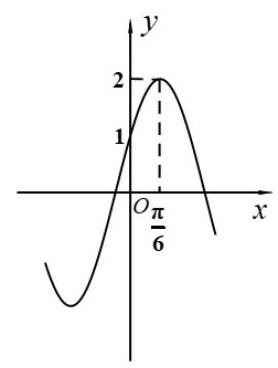
\includegraphics[max width=0.2\textwidth]{images/bo_d6dceus601uc73dvofhg_34_1117_532_278_368_0.jpg}
\end{center}
\hspace*{3em} 

【答案】(1) \(y = 2\sin \left( {{2x} + \frac{\pi }{6}}\right)\) (2) \(\bigtriangleup {ABC}\) 是等边三角形.

【解析】(1) 由题意， \(A = 2,2\sin \varphi  = 1\) ，由 \(\left| \varphi \right|  < \frac{\pi }{2}\) ，得 \(\varphi  = \frac{\pi }{6}\) ，

由 \(2\sin \left( {\frac{\pi }{6}\omega  + \frac{\pi }{6}}\right)  = 2\) ,得 \(\omega  = 2 + {12k}\left( {k \in  \mathrm{Z}}\right)\) ,

由图像可知, \(\frac{T}{4} = \frac{\pi }{6},T = \frac{2\pi }{\omega } > \frac{2\pi }{3}\) ,因此 \(0 < \omega  < 3\) ,由此可得 \(\omega  = 2\) ,

故 \(y = f\left( x\right)\) 的解析式为 \(y = 2\sin \left( {{2x} + \frac{\pi }{6}}\right)\) ;

(2)由题意， \(2\sin \left( {{2B} + \frac{\pi }{6}}\right)  = 1\) ， \(B \in  \left( {0,\pi }\right)\) ，得 \(B = \frac{\pi }{3}\) ，由 \(a\) 、 \(b\) 、 \(c\) 成等差数列得 \(b = \frac{a + c}{2}\) ， 由余弦定理得 \({b}^{2} = {a}^{2} + {c}^{2} - {2ac}\cos B,{\left( \frac{a + c}{2}\right) }^{2} = {a}^{2} + {c}^{2} - {2ac}\cos \frac{\pi }{3}\) , \(\frac{{a}^{2} + {c}^{2} + {2ac}}{4} = {a}^{2} + {c}^{2} - {ac},{\left( a - c\right) }^{2} = 0,a = c\) ,又 \(B = \frac{\pi }{3}\) ,所以 \(\bigtriangleup {ABC}\) 是等边三角形.

\section*{4.3 函数性质}

1.【2025.12 杨浦高三一模 2】函数 \(y = 3\sin \left( {{2x} + \frac{\pi }{6}}\right)\) 的最小正周期为\_\_\_\_\_. 答案: \(\pi\)

【解析】最小正周期为 \(T = \frac{2\pi }{2} = \pi\)

2.【2025.12 徐汇高三一模 3】函数 \(y = \sin x + \cos x\) 的值域为\_\_\_\_\_.

【答案】化简得 \(y = \sqrt{2}\sin \left( {x + \frac{\pi }{4}}\right)  \in  \left\lbrack  {-\sqrt{2},\sqrt{2}}\right\rbrack\) .

3.【2025.12 崇明高三一模 4】函数 \(y = 2\cos \left( {{\omega x} - \frac{\pi }{3}}\right) \left( {\omega  > 0}\right)\) 的最小正周期是 \(\pi\) ，则 \(\omega  =\) \_\_\_\_\_.

【答案】 2

【解析】依题意可得: 为 \(T = \frac{2\pi }{\omega } = \pi\) ,解得 \(\omega  = 2 \cdot  3 <\)

4.【2025.12 普陀高三一模 13】下列函数中，周期为 \(\pi\) 的奇函数是( ).

A. \(y = \left| {\sin x}\right|\) B. \(y = {\cos }^{2}x - {\sin }^{2}x\) C. \(y = \cos \left( {\frac{\pi }{2} - x}\right)\) D. \(y = \frac{\sin {2x}}{1 + \cos {2x}}\)

【答案】D. \(>  <\)

5.【2025.12 虹口高三一模 14】已知 \(f\left( x\right)  = \left\{  \begin{array}{ll} \tan x & x > 0 \\   - f\left( {x + \pi }\right) & x < 0 \end{array}\right.\) ,若 \(f\left( \alpha \right)  = \sqrt{3}\) ,则实数 \(\alpha\) 的取值可以是( )

A. \(- \frac{2\pi }{3}\) B. \(- \frac{\pi }{3}\) C. \(\frac{\pi }{6}\) D. \(\frac{2\pi }{3}\)

【答案】B

【解析】当 \(\alpha  > 0\) 时, \(f\left( \alpha \right)  = \tan \alpha  = \sqrt{3}\) ,则 \(\alpha  = \frac{\pi }{3} + {k\pi }\left( {k \in  \mathbb{N}}\right)\) ,排除 \(\mathrm{C}/\mathrm{D}\) ;

当 \(\alpha  < 0\) 时, \(f\left( \alpha \right)  =  - \tan \left( {\alpha  + \pi }\right)  = \sqrt{3}\) ,此时 \(\alpha  =  - \frac{\pi }{3} + {k\pi }\left( {k \in  \mathbb{N}}\right)\) ,所以 \(\alpha  =  - \frac{\pi }{3}\) 是可能的, 选 B. 2

6.【2025.12 嘉定高三一模 14】函数 \(y = 1 - 2{\cos }^{2}\left( {x + \frac{\pi }{4}}\right)\) 是( )

A. 最小正周期为 \({2\pi }\) 的奇函数 B. 最小正周期为 \({2\pi }\) 的偶函数

C. 最小正周期为 \(\pi\) 的奇函数 D. 最小正周期为 \(\pi\) 的偶函数

【答案】C

【解析】先化简得: \(y = 1 - 2{\cos }^{2}\left( {x + \frac{\pi }{4}}\right)  =  - \cos 2\left( {x + \frac{\pi }{4}}\right)  =  - \cos \left( {{2x} + \frac{\pi }{2}}\right)  = \sin {2x}\) , \(\therefore \mathrm{C}\) 正确. \(\approx\)

7.【2025.12 青浦高三一模 17】已知直线 \(x = \frac{\pi }{6}\) 是函数 \(f\left( x\right)  = \sin \left( {{2x} + \varphi }\right) \left( {\left| \varphi \right|  < \frac{\pi }{2}}\right)\) 的一条对称轴.

(1)求函数 \(y = f\left( x\right)\) 的表达式；

(2)设函数 \(g\left( x\right)  = f\left( {x - \frac{\pi }{12}}\right)  + f\left( {x + \frac{\pi }{6}}\right)\) ，求 \(y = g\left( x\right)\) 在 \(\left\lbrack  {-\frac{\pi }{4},\frac{\pi }{4}}\right\rbrack\) 上的最大值和最小值.

【答案】(1) \(f\left( x\right)  = \sin \left( {{2x} + \frac{\pi }{6}}\right)\) (2)最大值为 \(\sqrt{2}\) ，最小值为 -1

【解析】(1) 直线 \(x = \frac{\pi }{6}\) 是函数 \(f\left( x\right)  = \sin \left( {{2x} + \varphi }\right) \left( {\left| \varphi \right|  < \frac{\pi }{2}}\right)\) 的一条对称轴, 所以 \(2 \times  \frac{\pi }{6} + \varphi  = \frac{\pi }{2} + {k\pi },k \in  \mathbf{Z}\) ,解得 \(\varphi  = \frac{\pi }{6} + {k\pi },k \in  \mathbf{Z}\) ,由 \(\left| \varphi \right|  < \frac{\pi }{2}\) 可得 \(\varphi  = \frac{\pi }{6}\) , 所以 \(f\left( x\right)  = \sin \left( {{2x} + \frac{\pi }{6}}\right)\)

(2) \(g\left( x\right)  = f\left( {x - \frac{\pi }{12}}\right)  + f\left( {x + \frac{\pi }{6}}\right)  = \sin \left\lbrack  {2\left( {x - \frac{\pi }{12}}\right)  + \frac{\pi }{6}}\right\rbrack   + \sin \left\lbrack  {2\left( {x + \frac{\pi }{6}}\right)  + \frac{\pi }{6}}\right\rbrack\)

\(= \sin {2x} + \cos {2x} = \sqrt{2}\sin \left( {{2x} + \frac{\pi }{4}}\right)\)

令 \(t = {2x} + \frac{\pi }{4}\) ,由 \(x \in  \left\lbrack  {-\frac{\pi }{4},\frac{\pi }{4}}\right\rbrack  ,t \in  \left\lbrack  {-\frac{\pi }{4},\frac{3\pi }{4}}\right\rbrack\)

因为函数 \(y = \sqrt{2}\sin t\) 在区间 \(\left\lbrack  {-\frac{\pi }{4},\frac{\pi }{2}}\right\rbrack\) 上严格增,在区间 \(\left\lbrack  {\frac{\pi }{2},\frac{3\pi }{4}}\right\rbrack\) 上严格减,

又 \(\sqrt{2}\sin \left( {-\frac{\pi }{4}}\right)  =  - 1,\sqrt{2}\sin \frac{\pi }{2} = \sqrt{2},\sqrt{2}\sin \frac{3\pi }{4} = 1\) ,所以 \(g{\left( x\right) }_{\max } = \sqrt{2},g{\left( x\right) }_{\min } =  - 1\) ,

即 \(g\left( x\right)\) 在 \(\left\lbrack  {-\frac{\pi }{4},\frac{\pi }{4}}\right\rbrack\) 上的最大值为 \(\sqrt{2}\) ,最小值为 \(- 1 \ll\)

8.【2025.12 浦东高三一模 17】已知函数 \(y = f\left( x\right)\) ,其中 \(f\left( x\right)  = \cos \left( {{2x} - \frac{\pi }{3}}\right)\) .

(1)求函数 \(y = f\left( x\right)\) 的最小正周期及单调减区间.

(2)求函数 \(y = 2{\sin }^{2}x + f\left( x\right)\) ， \(x \in  \left\lbrack  {-\frac{\pi }{6},\frac{\pi }{3}}\right\rbrack\) 的最大值，并求出取得最大值时 \(x\) 的值.

【答案】( 1 ) \(\left\lbrack  {{k\pi } + \frac{\pi }{6},{k\pi } + \frac{2\pi }{3}}\right\rbrack  \left( {k \in  \mathbf{Z}}\right)\) (2)最大值是 2，此时 \(x = \frac{\pi }{3}\) .

【解析】(1) 由题意,函数 \(y = \cos \left( {{2x} - \frac{\pi }{3}}\right)\) 的最小正周期 \(T = \frac{2\pi }{2} = \pi\) , .3 分

由余弦函数的单调性可知,当 \({2k\pi } \leq  {2x} - \frac{\pi }{3} \leq  {2k\pi } + \pi \left( {k \in  \mathbf{Z}}\right)\) ,即

\({k\pi } + \frac{\pi }{6} \leq  x \leq  {k\pi } + \frac{2\pi }{3}\left( {k \in  \mathbf{Z}}\right)\) 时,函数 \(y = \cos \left( {{2x} - \frac{\pi }{3}}\right)\) 是严格减函数,即 \(y = f\left( x\right)\) 的单调减区间是 \(\left\lbrack  {{k\pi } + \frac{\pi }{6},{k\pi } + \frac{2\pi }{3}}\right\rbrack  \left( {k \in  \mathbf{Z}}\right)\) . .6 分

(2)由题意，函数 \(y = 2{\sin }^{2}x + \cos \left( {{2x} - \frac{\pi }{3}}\right)  = 1 - \cos {2x} + \frac{1}{2}\cos {2x} + \frac{\sqrt{3}}{2}\sin {2x} \; = \frac{\sqrt{3}}{2}\sin {2x} - \frac{1}{2}\cos {2x} + 1\) .9 分 \(= \sin \left( {{2x} - \frac{\pi }{6}}\right)  + 1\) .11 分

令 \(u = {2x} - \frac{\pi }{6}\) ,则 \(y = \sin u + 1\) . 由 \(x \in  \left\lbrack  {-\frac{\pi }{6},\frac{\pi }{3}}\right\rbrack\) ,有 \(- \frac{\pi }{2} \leq  {2x} \leq  \frac{\pi }{2}\) ,即 \(u \in  \left\lbrack  {-\frac{\pi }{2},\frac{\pi }{2}}\right\rbrack\) .

由正弦函数的性质可知, \(y = \sin u + 1\) 在 \(\left\lbrack  {-\frac{\pi }{2},\frac{\pi }{2}}\right\rbrack\) 上是严格增函数 12 分

又因为 \(\sin \frac{\pi }{2} = 1\) ,所以 \(y = \sin u + 1\) 的最大值是 2,此时 \(u = \frac{\pi }{2}\) ,即 \(x = \frac{\pi }{3}\) .

综上,函数 \(y = 2{\sin }^{2}x + f\left( x\right) ,x \in  \left\lbrack  {-\frac{\pi }{6},\frac{\pi }{3}}\right\rbrack\) 的最大值是 2,此时 \(x = \frac{\pi }{3}\) . 14 分

9.【2025.12 长宁高三一模 18】已知函数 \(f\left( x\right)  = \cos {\omega x}\left( {\omega  > 0}\right)\) .

(1)若函数 \(y = f\left( x\right)\) 的最小正周期为 \(\pi\) ，求 \(\omega\) 的值及 \(y = f\left( x\right)\) 的单调减区间；

(2)设 \(\omega  = 1,g\left( x\right)  = f\left( {2x}\right)  - {2f}\left( x\right) f\left( {x + \frac{\pi }{2}}\right)\) ，求函数 \(y = g\left( x\right)\) 在区间 \(\left\lbrack  {0,\frac{\pi }{2}}\right\rbrack\) 上的值域.

【答案】(1) \(\omega  = 2,\left\lbrack  {{k\pi },{k\pi } + \frac{\pi }{2}}\right\rbrack  \left( {k \in  \mathbf{Z}}\right)\) (2) \(\left\lbrack  {-1,\sqrt{2}}\right\rbrack\)

【解析】(1) 因为函数 \(y = f\left( x\right)\) 的最小正周期为 \(\pi\) ,

所以 \(\frac{2\pi }{\omega } = \pi\) ,得 \(\omega  = 2,f\left( x\right)  = \cos {2x}\) .

由 \({2k\pi } \leq  {2x} \leq  {2k\pi } + \pi ,k \in  \mathbf{Z}\) ,得 \({k\pi } \leq  x \leq  {k\pi } + \frac{\pi }{2},k \in  \mathbf{Z}\) ,

所以函数 \(y = f\left( x\right)\) 的单调减区间为 \(\left\lbrack  {{k\pi },{k\pi } + \frac{\pi }{2}}\right\rbrack  \left( {k \in  \mathbf{Z}}\right)\) .

(2) \(g\left( x\right)  = \cos {2x} - 2\cos x\cos \left( {x + \frac{\pi }{2}}\right)  = \cos {2x} + \sin {2x} = \sqrt{2}\sin \left( {{2x} + \frac{\pi }{4}}\right)\) .

当 \(x \in  \left\lbrack  {0,\frac{\pi }{2}}\right\rbrack\) 时, \({2x} + \frac{\pi }{4} \in  \left\lbrack  {\frac{\pi }{4},\frac{3\pi }{4}}\right\rbrack  ,\sin \left( {{2x} + \frac{3\pi }{4}}\right)  \in  \left\lbrack  {-\frac{\sqrt{2}}{2},1}\right\rbrack\) .

所以求函数 \(y = g\left( x\right)\) 在区间 \(\left\lbrack  {0,\frac{\pi }{2}}\right\rbrack\) 上的值域为 \(\left\lbrack  {-1,\sqrt{2}}\right\rbrack\) . \(>\)

10.【2025.12 虹口高三一模 18】已知 \(\omega  > 0,\left| \varphi \right|  \leq  \pi\) ,设 \(f\left( x\right)  = \cos \left( {{\omega x} + \varphi }\right)\) .

(1)当 \(\omega  = 2\) ， \(\varphi  = \frac{\pi }{4}\) 时，试判断函数 \(y = f\left( x\right)\) 的奇偶性，并说明理由；

(2)当 \(\varphi  =  - \frac{\pi }{2}\) 且函数 \(y = f\left( x\right)\) 的最小正周期为 \({2\pi }\) 时,若在 \(\bigtriangleup  {ABC}\) 中， \({\sin }^{2}A + {\sin }^{2}C - {\sin }^{2}B = \sin A\sin C\) ,求 \(f\left( A\right)  + f\left( C\right)\) 的取值范围.

【答案】(1)非奇非偶函数

(2) \(\left( {\frac{\sqrt{3}}{2},\sqrt{3}}\right\rbrack\)

【解析】(1) \(f\left( x\right)  = \cos \left( {{2x} + \frac{\pi }{4}}\right)\) ,定义域为 \(\mathrm{R}\) . 则 \(f\left( 0\right)  = \frac{\sqrt{2}}{2} \neq  0\) . 2 分 \(f\left( \frac{\pi }{4}\right)  = \cos \left( \frac{3\pi }{4}\right)  =  - \frac{\sqrt{2}}{2},\;f\left( {-\frac{\pi }{4}}\right)  = \cos \left( {-\frac{\pi }{4}}\right)  = \frac{\sqrt{2}}{2},\;f\left( \frac{\pi }{4}\right)  \neq  f\left( {-\frac{\pi }{4}}\right) .\;4\) 分所以函数 \(y = f\left( x\right)\) 既不是奇函数,又不是偶函数. 6 分

( 2 )由于 \(T = \frac{2\pi }{\omega } = {2\pi }\) ，即 \(\omega  = 1\) ，所以 \(f\left( x\right)  = \cos \left( {x - \frac{\pi }{2}}\right)  = \sin x\) . 8 分

由正弦定理, \({a}^{2} + {c}^{2} - {b}^{2} = {ac}\) ,所以 \(\cos B = \frac{{a}^{2} + {c}^{2} - {b}^{2}}{2ac} = \frac{1}{2}\) ,故 \(B = \frac{\pi }{3}\) . 10 分

故 \(A + C = \frac{2}{3}\pi\) ,则 \(f\left( A\right)  + f\left( C\right)  = \sin \left( {\frac{2}{3}\pi  - C}\right)  + \sin C = \frac{3}{2}\sin C + \frac{\sqrt{3}}{2}\cos C\)

\(= \sqrt{3}\sin \left( {C + \frac{\pi }{6}}\right) ,C \in  \left( {0,\frac{2}{3}\pi }\right) .{12}\) 分

则 \(C + \frac{\pi }{6} \in  \left( {\frac{\pi }{6},\frac{5\pi }{6}}\right)\) ,故 \(\sin \left( {C + \frac{\pi }{6}}\right)  \in  \left( {\frac{1}{2},1}\right\rbrack\) ,则 \(f\left( A\right)  + f\left( C\right)  \in  \left( {\frac{\sqrt{3}}{2},\sqrt{3}}\right\rbrack\) . 14 分 \(\ll\)

11.【2025.12 静安高三一模 18】已知函数 \(f\left( x\right)  = 4\sin \left( {{\omega x} + \frac{\pi }{4}}\right)  \cdot  \cos {\omega x} - \sqrt{2}\left( {\omega  > 0}\right)\) .

(1)将函数 \(y = f\left( x\right)\) 化为 \(y = A\sin \left( {{kx} + \varphi }\right) \left( {A > 0,k > 0,\left| \varphi \right|  \leq  \frac{\pi }{2}}\right)\) 的形式，并指出这个函数的振幅和初始相位;

(2)若函数 \(y = f\left( x\right)\) 的最小正周期为 \(\pi\) ，求 \(\omega\) 的值并求函数 \(y = f\left( x\right)\) 的值域.

【答案】(1) \(f\left( x\right)  = 2\sin \left( {{2\omega x} + \frac{\pi }{4}}\right)\) ,振幅 2,初始相位 \(\frac{\pi }{4}\) (2) \(\omega  = 1\) ，值域 \(\left\lbrack  {-2,2}\right\rbrack\)

【解析】(1) \(f\left( x\right)  = 4\sin \left( {{\omega x} + \frac{\pi }{4}}\right)  \cdot  \cos {\omega x} - \sqrt{2} = 2\sqrt{2}\sin {\omega x}\cos {\omega x} + 2\sqrt{2}{\cos }^{2}{\omega x} - \sqrt{2}\) , \(= \sqrt{2}\sin {2\omega x} + \sqrt{2}\cos {2\omega x} = 2\sin \left( {{2\omega x} + \frac{\pi }{4}}\right)\) 这个函数的振幅为 2,初始相位为 \(\frac{\pi }{4}\) .

(2)由 \(y = f\left( x\right)\) 的最小正周期为 \(\pi\) ，且 \(\omega  > 0\) ，故 \(\frac{2\pi }{2\omega } = \pi  \Rightarrow  \omega  = 1\) . 函数 \(y = f\left( x\right)\) 的值域为 \(\left\lbrack  {-2,2}\right\rbrack  . \propto\)

12.【2025.12 普陀高三一模 18】在 \(\bigtriangleup  {ABC}\) 中，内角 \(A\) ， \(B\) ， \(C\) 所对的边分别为 \(a\) ， \(b\) ， \(c\) ,且 \(a = \frac{\sqrt{3}}{3},b\sin {2A} = \sin B\) .

(1)求角 \(A\) 的大小；

(2)设 \(m \in  \mathbf{R},0 < \varphi  < \frac{\pi }{2}\) ，函数 \(y = f\left( x\right)\) 的表达式为 \(f\left( x\right)  = \tan \left( {{2x} + \varphi }\right)\) ，且 \(f\left( A\right)  =  - \sqrt{3}\) ，若在区间 \(\left( {-\frac{5\pi }{6},m}\right)\) 上恰有 3 次使得函数 \(f\left( x\right)\) 的值能取遍区间 \(\lbrack {2025}, + \infty )\) 内的所有值,求 \(m\) 的取值范围.

【答案】(1) \(A = \frac{\pi }{6}\) (2) \(\left\lbrack  {\frac{7\pi }{12},\frac{13\pi }{12}}\right)\)

【解析】(1) 由已知条件得, \(\frac{b}{\sin B} = \frac{1}{\sin {2A}} = \frac{1}{2\sin A\cos A}\) , .2 分

由正弦定理 \(\frac{a}{\sin A} = \frac{b}{\sin B}\) 得, \(\frac{a}{\sin A} = \frac{1}{2\sin A\cos A}\) , .4 分

又 \(\sin A > 0\) ,则 \(\cos A = \frac{1}{2a} = \frac{\sqrt{3}}{2}\) ,则 \(A = \frac{\pi }{6}\) . .6 分

( 2 )由 \(f\left( A\right)  =  - \sqrt{3}\) 得， \(\tan \left( {\frac{\pi }{3} + \varphi }\right)  =  - \sqrt{3}\) ，又 \(\varphi  \in  \left( {0,\frac{\pi }{2}}\right)\) ，则 \(\varphi  = \frac{\pi }{3}\) ， .2 分

又 \(x \in  \left( {-\frac{5\pi }{6},m}\right)\) ,则 \({2x} + \frac{\pi }{3} \in  \left( {-\frac{4\pi }{3},{2m} + \frac{\pi }{3}}\right)\) , .4 分

要在区间 \(\left( {-\frac{5\pi }{6},m}\right)\) 上恰有三次使得函数 \(f\left( x\right)  = \tan \left( {{2x} + \frac{\pi }{3}}\right)\) 的值能取遍 \(\lbrack {2025}, + \infty )\) 内的所有值,则 \(\frac{3\pi }{2} \leq  {2m} + \frac{\pi }{3} < \frac{5\pi }{2}\) ,即 \(\frac{7\pi }{12} \leq  m < \frac{13\pi }{12}\) ,

则所求的 \(m\) 的取值范围是 \(\left\lbrack  {\frac{7\pi }{12},\frac{13\pi }{12}}\right)\) . .8 分奖

\section*{4.4 综合应用}

1.【2025.12 青浦高三一模 15】对于实数 \(m \in  \left\lbrack  {-1,1}\right\rbrack\) ,定义集合 \({A}_{m} = \left\{  {x\left| {\;x = \sin \frac{\alpha }{2}}\right. ,\sin \alpha  = m}\right\}\) , 集合 \({A}_{m}\) 的元素个数为 \(\left| {A}_{m}\right|\) ,给出下列说法:

 \circled{1}  存在 \(m\) ，使得 \(\left| {A}_{m}\right|  = 1\) ；  \circled{2}  存在 \(m\) ，使得 \(\left| {A}_{m}\right|  = 2\) ；

 \circled{3}  存在 \(m\) ，使得 \(\left| {A}_{m}\right|  = 3\) ；  \circled{4}  存在 \(m\) ，使得 \(\left| {A}_{m}\right|  = 4\) .

其中正确的说法有( )个.

A. 1 B. 2 C. 3 D. 4

【答案】C

【解析】当 \(m = 0\) 时, \(\alpha  = {k\pi }\left( {k \in  \mathbb{Z}}\right)\) ,则 \(\frac{\alpha }{2} = \frac{k\pi }{2}\left( {k \in  \mathbb{Z}}\right)\) ,

\(\therefore\) 此时 \(x = \sin \frac{\alpha }{2} = 1\) 或0或 -1,即 \(\left| {A}_{m}\right|  = 3\) ;

当 \(m = 1\) 时, \(\alpha  = \frac{\pi }{2} + {2k\pi }\left( {k \in  \mathbb{Z}}\right)\) ,则 \(\frac{\alpha }{2} = \frac{\pi }{4} + {k\pi }\left( {k \in  \mathbb{Z}}\right)\) ,

\(\therefore\) 此时 \(x = \sin \frac{\alpha }{2} =  \pm  \frac{\sqrt{2}}{2}\) ,即 \(\left| {A}_{m}\right|  = 2\) ;

当 \(m = \frac{\sqrt{3}}{2}\) 时, \(\alpha  = \frac{\pi }{3} + {2k\pi }\left( {k \in  \mathbb{Z}}\right)\) 或 \(\frac{2\pi }{3} + {2k\pi }\left( {k \in  \mathbb{Z}}\right)\) ,

则 \(\frac{\alpha }{2} = \frac{\pi }{6} + {k\pi }\left( {k \in  \mathbb{Z}}\right)\) 或 \(\frac{\pi }{3} + {k\pi }\left( {k \in  \mathbb{Z}}\right)\) , \(\therefore\) 此时 \(x = \sin \frac{\alpha }{2} =  \pm  \frac{1}{2}\) 或 \(\pm  \frac{\sqrt{3}}{2}\) ,即 \(\left| {A}_{m}\right|  = 4\) .

2.【2025.12 松江高三一模 17】已知函数 \(y = A\sin \left( {{\omega x} + \varphi }\right) \left( {A,\omega  > 0,0 < \varphi  < \pi }\right)\) 的周期为 \(\pi\) , 在 \(x = \frac{\pi }{6}\) 时取到最大值 4,记 \(y = f\left( x\right)\) .

(1)求函数 \(y = f\left( x\right)\) 的表达式；

(2)若数列 \(\left\{  {a}_{n}\right\}\) 为等差数列， \({a}_{2} = f\left( 0\right)\) ， \({a}_{4} = f\left( \frac{\pi }{6}\right)\) ，记 \({b}_{n} = {2}^{{a}_{n}}\) ，求数列 \(\left\{  {b}_{n}\right\}\) 的前 \(n\) 项和 \({T}_{n}\) .

【答案】(1) \(y = 4\sin \left( {{2x} + \frac{\pi }{6}}\right)\) (2) \({T}_{n} = {2}^{n + 1} - 2\)

【解析】(1)由题意得: \(T = \frac{2\pi }{\omega } = \pi\) ，所以 \(\omega  = 2\) . -2 分

由函数在 \(x = \frac{\pi }{6}\) 时取得最大值 \(4,\therefore A = 4\) , -4 分

则 \(4\sin \left( {2 \times  \frac{\pi }{6} + \varphi }\right)  = 4,\therefore \sin \left( {\frac{\pi }{3} + \varphi }\right)  = 1\) ,

又 \(0 < \varphi  < \pi\) ，所以 \(\varphi  = \frac{\pi }{6}\) ， \(\therefore f\left( x\right)  = 4\sin \left( {{2x} + \frac{\pi }{6}}\right)\) . -6 分

( 2 ) \(\because {a}_{2} = f\left( 0\right)  = 2\) ， \({a}_{4} = f\left( \frac{\pi }{6}\right)  = 4\) ，数列 \(\left\{  {a}_{n}\right\}\) 为等差数列， \(\therefore {a}_{n} = n\) -8 分则 \({b}_{n} = {2}^{{a}_{n}} = {2}^{n}\) ,所以数列 \(\left\{  {b}_{n}\right\}\) 是以 2 为首项,2 为公比的等比数列, -10 分所以 \({T}_{n} = \frac{2\left( {1 - {2}^{n}}\right) }{1 - 2} = {2}^{n + 1} - 2\) . -14 分↵

3.【2025.12 金山高三一模 19】已知 \(f\left( x\right)  = 2\sin \left( {{\omega x} + \varphi }\right)\) (其中 \(\omega  > 0,\left| \varphi \right|  < \frac{\pi }{2}\) )，函数 \(y = f\left( x\right)\) 相邻的极小值点和极大值点分别为 \(- \frac{\pi }{3}\) 和 \(\frac{2\pi }{3}\) . 直线 \(l\) 为函数 \(y = f\left( x\right)\) 在 \(y\) 轴右侧与 \(y\) 轴距离最近的对称轴,且分别交函数 \(y = f\left( x\right)\) 的图像和 \(x\) 轴于 \(A\text{ 、 }B\) 两点,点 \(C\) 为线段 \({AB}\) 上一动点.

(1)求函数 \(y = f\left( x\right)\) 的表达式，并写出其严格增区间；

(2)设 \(\angle {BOC} = \theta\) ，记 \(L = {AC} + {2OC}\) ，请写出 \(L\) 关于 \(\theta\) 的函数表达式，并求 \(L\) 的最小值.

\begin{center}
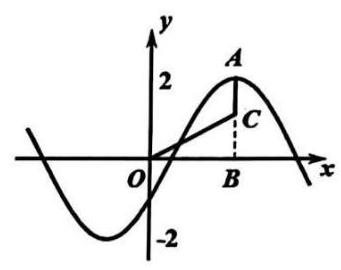
\includegraphics[max width=0.2\textwidth]{images/bo_d6dceus601uc73dvofhg_40_1059_1709_341_270_0.jpg}
\end{center}
\hspace*{3em} 

【答案】(1) \(f\left( x\right)  = 2\sin \left( {x - \frac{\pi }{6}}\right)\) ，严格增区间为 \(\left\lbrack  {{2k\pi } - \frac{\pi }{3},{2k\pi } + \frac{2\pi }{3}}\right\rbrack  ,k \in  \mathbb{Z}\)

(2) \(L = {2OC} + {AC} = \frac{2\pi }{3}\left( {\frac{2}{\cos \theta } - \tan \theta }\right)  + 2,\theta  \in  \left\lbrack  {0,\arctan \frac{3}{\pi }}\right\rbrack\) ，当 \(\theta  = \frac{\pi }{6}\) 时， \({L}_{\min } = \frac{2\sqrt{3}}{3}\pi  + 2\)

【解析】(1) 由题意得: \(T = 2\left( {\frac{2\pi }{3} + \frac{\pi }{3}}\right)  = {2\pi }\) ，所以 \(\omega  = 1\) . .2 分因为函数 \(y = f\left( x\right)\) 极大值点分别为 \(\frac{2\pi }{3}\) ,所以 \(\sin \left( {\frac{2\pi }{3} + \varphi }\right)  = 1\) ,所以 \(\varphi  =  - \frac{\pi }{6}\) .4 分所以 \(f\left( x\right)  = 2\sin \left( {x - \frac{\pi }{6}}\right)\) . 函数的严格增区间为 \(\left\lbrack  {{2k\pi } - \frac{\pi }{3},{2k\pi } + \frac{2\pi }{3}}\right\rbrack  ,k \in  \mathbb{Z}\) .6 分

(2)由题意得: \({OC} = \frac{2\pi }{3\cos \theta },{AC} = 2 - \frac{2\pi }{3}\tan \theta\) . .8 分

此时 \(L = {2OC} + {AC} = \frac{2\pi }{3}\left( {\frac{2}{\cos \theta } - \tan \theta }\right)  + 2,\theta  \in  \left\lbrack  {0,\arctan \frac{3}{\pi }}\right\rbrack\) . .10 分

所以 \({L}^{\prime } = \frac{2\pi }{3} \times  \frac{2\sin \theta  - 1}{{\cos }^{2}\theta }\) . .12 分

\begin{center}
\adjustbox{max width=\textwidth}{
\begin{tabular}{|c|c|c|c|}
\hline
\(x\) & \(\lbrack 0,\frac{\pi }{6})\) & \(\frac{\pi }{6}\) & \(\left( {\frac{\pi }{6},\arctan \frac{3}{\pi }}\right\rbrack\) \\
\cline{1-4}
\(L\) & 负 & 零 & 正 \\
\cline{1-4}
\(L\) & 严格减 & 极小值为 \(\frac{2\sqrt{3}}{3}\pi  + 2\) & 严格增 \\
\cline{1-4}
\hline
\end{tabular}
}
\end{center}

所以当 \(\theta  = \frac{\pi }{6}\) 时, \({L}_{\min } = \frac{2\sqrt{3}}{3}\pi  + 2\) . .14 分

\section*{第五章 数列}

\section*{【知识梳理】}

 \circled{1}  等差数列: 设 \(n\) 为正整数,若数列 \(\left\{  {a}_{n}\right\}\) 满足 \({a}_{n + 1} - {a}_{n} = d\) ,则 \(\left\{  {a}_{n}\right\}\) 为等差数列;

等差数列 \(\left\{  {a}_{n}\right\}\) 的通项公式: \({a}_{n} = {a}_{1} + \left( {n - 1}\right) d = {an} + b\) (一次函数);

等差数列 \(\left\{  {a}_{n}\right\}\) 的前 \(n\) 项和的公式: \({S}_{n} = \frac{n\left( {{a}_{1} + {a}_{n}}\right) }{2} = n{a}_{1} + \frac{n\left( {n - 1}\right) }{2}d = a{n}^{2} + {bn}\) (二次函数不带常数 C).

 \circled{2}  等比数列: 设 \(n\) 为正整数,若数列 \(\left\{  {a}_{n}\right\}\) 满足 \(\frac{{a}_{n + 1}}{{a}_{n}} = q\left( {q \neq  0}\right)\) ,则 \(\left\{  {a}_{n}\right\}\) 为等比数列; 等比数列 \(\left\{  {a}_{n}\right\}\) 的通项公式: \({a}_{n} = {a}_{1}{q}^{n - 1}\) ;

等比数列 \(\left\{  {a}_{n}\right\}\) 前 \(n\) 项和的公式: \({S}_{n} = \left\{  {\begin{matrix} n{a}_{1} & \left( {q = 1}\right) \\  \frac{{a}_{1}\left( {1 - {q}^{n}}\right) }{1 - q} & \left( {q \neq  1}\right)  \end{matrix} = A - A{q}^{n}\;\left( {q \neq  1}\right) }\right.\) .

 \circled{3} 用数学归纳法证明命题的一般步骤是:

(1)证明当 \(n\) 取第一个值 \({n}_{0}\) ( \({n}_{0}\) 为正整数)时，命题成立；

(2)假设当 \(n = k\left( {k \geq  {n}_{0},k}\right.\) 为正整数 \()\) 时命题成立,证明当 \(n = k + 1\) 时命题也成立.

 \circled{4} 主要性质: (1) \(p + q = m + n \Rightarrow  {a}_{p} + {a}_{q} = {a}_{m} + {a}_{n}\) ;

(2) \(p,q,r\) 成等差数列 \(\Rightarrow  {a}_{p},{a}_{q},{a}_{r}\) 成等差数列.

(3) \({S}_{m}\) ， \({S}_{2m} - {S}_{m}\) ， \({S}_{3m} - {S}_{2m}\) ，成等差数列.

\section*{5.1 等差数列}

1.【 2025.12 长宁高三一模 3】在等差数列 \(\left\{  {a}_{n}\right\}\) 中， \({a}_{2} = 1\) ，公差 \(d = 2\) ， \({a}_{n} = {11}\) ，则 \(n =\) \_\_\_\_\_.

【答案】 \({a}_{n} = {a}_{2} + \left( {n - 2}\right) d\) ,代入计算得 \(n = 7\) .

2.【2025.12 青浦高三一模 5】设等差数列 \(\left\{  {a}_{n}\right\}\) 的前 \(n\) 项和为 \({S}_{n}\) ,若 \({S}_{5} = 5,{a}_{2} = 0\) ,则 \({a}_{8} =\) \_\_\_\_\_.

【答案】 6

【解析】依题意可得: \({S}_{5} = 5{a}_{3} = 5\) 得 \({a}_{3} = 1\) ,结合 \({a}_{2} = 0,\therefore {a}_{n} = n - 2,\therefore {a}_{8} = 6\) .

3.【2025.12 普陀高三一模 5】设 \(n \geq  1,n \in  \mathbf{N}\) ， \({S}_{n}\) 是等差数列 \(\left\{  {a}_{n}\right\}\) 的前 \(n\) 项和，若 \({a}_{3} = 1\) ， \({S}_{7} = 3{a}_{6}\) ，则该等差数列的公差为\_\_\_\_\_.

【答案】 2

【解析】由 \({S}_{7} = 3{a}_{6}\) 得 \(7{a}_{4} = 3{a}_{6}\) ,即 \(7\left( {{a}_{3} + d}\right)  = 3\left( {{a}_{3} + {3d}}\right)\) ,将 \({a}_{3} = 1\) 代入得 \(d = 2\) .

4.【2025.12 静安高三一模 6】设等差数列 \(\left\{  {a}_{n}\right\}\) 的前 \(n\) 项和为 \({S}_{n}\) ( \(n\) 为正整数)，首项 \({a}_{1} = \frac{3}{2},{a}_{6} = 9\) ,则 \({S}_{7} =\) \_\_\_\_\_.

【答案】 42

【解析】依题意可得: \({a}_{n} = \frac{3}{2}n,\therefore {a}_{7} = \frac{21}{2}\) ,从而 \({S}_{7} = \frac{7\left( {{a}_{1} + {a}_{7}}\right) }{2} = {42}\) .

5.【2025.12 崇明高三一模 6】已知等差数列 \(\left\{  {a}_{n}\right\}\) 首项为 \({a}_{1} = 1\) ，公差 \(d = 2\) ，则其前 6 项和 \({S}_{6} =\) \_\_\_\_\_.

【答案】36

【解析】直接套公式 \({S}_{n} = \frac{d}{2}{n}^{2} + \left( {{a}_{1} - \frac{d}{2}}\right) n\) 得 \({S}_{6} = {36}\) .

6.【2025.12 金山高三一模 9】在公差不为 0 的等差数列 \(\left\{  {a}_{n}\right\}\) 中,若 \({a}_{3}\) 是 \({a}_{s}\) 与 \({a}_{t}\) 的等差中项, 则 \(\frac{1}{s} + \frac{4}{t}\) 的最小值为\_\_\_\_\_.

【答案】 \(\frac{3}{2}\)

【解析】依题意有 \({a}_{s} + {a}_{t} = 2{a}_{3},\therefore s + t = 6\) .

\(\therefore \frac{1}{s} + \frac{4}{t} = \frac{1}{6}\left( {\frac{1}{s} + \frac{4}{t}}\right) \left( {s + t}\right)  = \frac{1}{6}\left( {5 + \frac{t}{s} + \frac{4s}{t}}\right)  \geq  \frac{1}{6}\left( {5 + 2\sqrt{\frac{t}{s} \cdot  \frac{4s}{t}}}\right)  = \frac{3}{2}\) .

当且仅当 \(\frac{t}{s} = \frac{4s}{t}\) ,即 \(s = 2,t = 4\) 时,等号成立, \(\therefore \frac{1}{s} + \frac{4}{t}\) 的最小值为 \(\frac{3}{2}.3 <\)

7.【2025.12 黄浦高三一模 10】已知数列 \(\left\{  {a}_{n}\right\}\) 是公差为 2 的等差数列,数列 \(\lg {a}_{1},\lg {a}_{k},\lg {a}_{7}\) 也为等差数列,且 \(k \in  \{ 3,4,5\}\) ,则 \({a}_{1} =\) \_\_\_\_\_.

【答案】 \({a}_{1} = 4\)

【解析】依题意得 \(2\lg {a}_{k} = \lg {a}_{1} + \lg {a}_{7} = \lg \left( {{a}_{1}{a}_{7}}\right)\) , \(\therefore {a}_{k}{}^{2} = {a}_{1}{a}_{7} \Rightarrow  {\left\lbrack  {a}_{1} + \left( k - 1\right) d\right\rbrack  }^{2} = {a}_{1}\left( {{a}_{1} + {6d}}\right)\) .

当 \(k = 3\) 时,代入解得 \({a}_{1} = 4\) ; 当 \(k = 4\) 时,无解; 当 \(k = 5\) 时,代入解得 \({a}_{1} =  - {16}\) (舍); 综上所述: \({a}_{1} = 4 \cdot  3 <\)

8.【2025.12 闵行高三一模 15】从等差数列:1,2,3, \(\cdots ,{1000}\) 中取出若干数字按先后顺序构成数列 \(\left\{  {a}_{n}\right\}\) . 第一次取出数字“1”，然后从取出的“1”开始往后数 2 个数，再取出数到 2 的数字“3”，...，以此类推，如果某次取出的是数字“ \({a}_{k}\) ”，则下一次从取出的“ \({a}_{k}\) ”开始往后数 \(k + 1\) 个数,再取出数到 \(k + 1\) 的数字“ \({a}_{k + 1}\) ”; 当往后数的数字个数小于“ \(k + 1\) ”时,结束取数. 那么 \(\left\{  {a}_{n}\right\}\) 的最后一项是( ).

A. 6 B. 990 C. 999 D. 1000

【答案】B

【解析】由题知: \({a}_{1} = 1,{a}_{2} = 3,{a}_{3} = 6,\ldots\) ,所以 \({a}_{k} = \frac{k\left( {k + 1}\right) }{2}\)

所以 \(\frac{k\left( {k + 1}\right) }{2} \leq  {1000} \Rightarrow  k \leq  {44.2} \Rightarrow  k = {44}\) ,所以 \(\left\{  {a}_{n}\right\}\) 的最后一项是 990,故选: B.S.

9.【2025.12 奉贤高三一模 16】已知等差数列 \(\left\{  {a}_{n}\right\}\) 的公差不为零, \({S}_{n}\) 为其前 \(n\) 项和,存在正整数 \(k\) 满足 \({S}_{k} = 0\) ,有两个命题:  \circled{1} : 设数列公差 \(d\) ,则 \(d \cdot  {S}_{1} < 0\) .

 \circled{2} : \(i\text{ 、 }j\) 均是小于 \(k\) 的正整数,则 \({S}_{i} \cdot  {S}_{j} = {S}_{k - i}{S}_{k - j}\) .

A. 命题 \circled{1}  \circled{2} 都是真命题 B. 命题 \circled{1} 是真命题，命题 \circled{2} 是假命题

C. 命题 \circled{1}  \circled{2} 都是假命题 D. 命题 \circled{1} 是假命题，命题 \circled{2} 是真命题

以上判断正确的是( )

【答案】D

【解析】对于命题 \circled{1} : 根据 \({S}_{k} = 0\) 得 \(\frac{d}{2}{k}^{2} + \left( {{a}_{1} - \frac{d}{2}}\right) k = 0\) ,解得 \(k = 1 - \frac{2{a}_{1}}{d} \geq  1,\therefore \frac{{a}_{1}}{d} \leq  0\) , \(\therefore\) 当 \({a}_{1} = 0\) 时, \circled{1} 为假命题;

对命题 \circled{2} :由 \({S}_{n} = \frac{d}{2}{n}^{2} + \left( {{a}_{1} - \frac{d}{2}}\right) n\) 可知:当 \({S}_{k} = 0\) 时，该抛物线的对称轴为 \(\frac{k}{2}\) .

所以 \({S}_{i} = {S}_{k - i},{S}_{j} = {S}_{k - j}\) ,此时 \({S}_{i}{S}_{j} = {S}_{k - i} \cdot  {S}_{k - j}\) 成立，故 \circled{2} 为真命题.

\section*{5.2 等比数列}

1.【2025.12 宝山高三一模 3】已知数列 \(\left\{  {a}_{n}\right\}\) 为等比数列,且 \({a}_{1} = 3\) ,公比 \(q = 2\) ,则该数列的前 4 项的和等于\_\_\_\_\_.

【答案】 \({S}_{4} = \frac{{a}_{1}\left( {1 - {q}^{4}}\right) }{1 - q} = {45}\) .

2.【 2025.12 奉贤高三一模 5】已知等比数列 \(\left\{  {a}_{n}\right\}\) 的各项均为正数,若 \({a}_{1} + {a}_{3} = {16},{a}_{2} + {a}_{4} = 4\) , 则该等比数列 \(\left\{  {a}_{n}\right\}\) 的公比为\_\_\_\_\_.

【答案】 \(q = \frac{1}{4}\)

【解析】设公比为 \(q\) ,则依题意可得 \(\left\{  \begin{array}{l} {a}_{1} + {a}_{3} = {a}_{1}\left( {1 + {q}^{2}}\right)  = {16} \\  {a}_{2} + {a}_{4} = {a}_{1}\left( {1 + {q}^{2}}\right) q = 4 \end{array}\right.\) ,两式相比得 \(q = \frac{1}{4}\) .

3.【2025.12 闵行高三一模 8】已知 \(\left\{  {a}_{n}\right\}\) 是等比数列，若 \({a}_{1}\) 、 \({a}_{5}\) 是函数 \(y = {x}^{2} + {3x} + 1\) 的两个零点,则 \({a}_{3} =\) \_\_\_\_\_.

【答案】 -1

【解析】由题知: \({x}^{2} + {3x} + 1 = 0\) 的两根为 \({a}_{1}\text{ 、 }{a}_{5}\) ,所以 \({a}_{1} + {a}_{5} =  - 3,{a}_{1} \cdot  {a}_{5} = 1\) , 所以 \({a}_{1} < 0,{a}_{5} < 0\) ,因为 \(\left\{  {a}_{n}\right\}\) 是等比数列,所以 \({a}_{1} \cdot  {a}_{5} = {a}_{3}{}^{2} = 1 \Rightarrow  {a}_{3} =  - 1 \ll\)

\section*{5.3 前 \(\mathrm{n}\) 项和}

【2025.12 杨浦高三一模 9】等差数列 \(\left\{  {a}_{n}\right\}\) 的公差不为 0,前 \(n\) 项和为 \({S}_{n}\) ,若 \({a}_{3},{a}_{5},{a}_{8}\) 成等比数列,则 \(\frac{{S}_{11}}{{a}_{10}} =\) \_\_\_\_\_.

【答案】7

【解析】依题意可得 \({a}_{5}{}^{2} = {a}_{3} \cdot  {a}_{8}\) ,即 \({\left( {a}_{1} + 4d\right) }^{2} = \left( {{a}_{1} + {2d}}\right)  \cdot  \left( {{a}_{1} + {7d}}\right)\) ,化简得 \({a}_{1} = {2d}\) , \(\therefore\) 通项公式为 \({a}_{n} = {a}_{1} + \left( {n - 1}\right) d = \left( {n + 1}\right) d,\therefore {a}_{10} = {11d},{S}_{11} = {11}{a}_{6} = {77d}\) ,故 \(\frac{{S}_{11}}{{a}_{10}} = 7 \gg\)

\section*{5.4 单调与递推}

1.【2025.12 嘉定高三一模 9】已知数列 \(\left\{  {a}_{n}\right\}\) 满足 \({a}_{1} = \frac{1}{3}\) ,且 \({a}_{n} = \frac{{a}_{n - 1}}{2{a}_{n - 1} + 1}\left( {n \geq  2}\right)\) ,则 \({a}_{100} =\) \_\_\_\_\_.

【答案】 \({a}_{100} = \frac{1}{201}\)

【解析】由 \({a}_{n} = \frac{{a}_{n - 1}}{2{a}_{n - 1} + 1}\) 可得 \(\frac{1}{{a}_{n}} = \frac{2{a}_{n - 1} + 1}{{a}_{n - 1}} = 2 + \frac{1}{{a}_{n - 1}}\) ,即 \(\frac{1}{{a}_{n}} - \frac{1}{{a}_{n - 1}} = 2\) , \(\therefore \left\{  \frac{1}{{a}_{n}}\right\}\) 为一个等差

数列,首项为 \(\frac{1}{{a}_{1}} = 3\) ,公差为 \(2,\therefore \frac{1}{{a}_{100}} = 3 + {99} \times  2 = {201}\) ,故 \({a}_{100} = \frac{1}{201}\) . 3 2 1

2.【2025.12 宝山高三一模 16】对任意正整数 \(n\) ，数列 \(\left\{  {a}_{n}\right\}\) 满足 \({a}_{n + 1} - {a}_{n} > 1\) ，则称该数列为“增长”数列.

命题 \circled{1} :存在 \({a}_{1} =  - 1\) 的等差数列 \(\left\{  {a}_{n}\right\}\) 为“增长”数列，且满足其 \(n\) 前项和 \({S}_{n} < \frac{{n}^{2} - {2n}}{2}\) .

命题 \circled{2} :存在各项均为正整数的等比数列 \(\left\{  {a}_{n}\right\}\) 为“增长”数列且 \(\left\{  \frac{{a}_{n}}{2}\right\}\) 不是“增长”数列，使得 \(\left\{  \frac{{a}_{n + 1}}{n + 1}\right\}\) 为“增长”数列. ( )

A.  \circled{1} 是真命题， \circled{2} 是真命题； B.  \circled{1} 是真命题， \circled{2} 是假命题；

C.  \circled{1} 是假命题， \circled{2} 是真命题； D.  \circled{1} 是假命题， \circled{2} 是假命题.

【答案】C

【解析】对 \circled{1} : 依题意可得: 此时等差数列 \(\left\{  {a}_{n}\right\}\) 的公差为 \(d = {a}_{n + 1} - {a}_{n} > 1\) ,

所以 \({S}_{n} = {a}_{1}n + \frac{d}{2}\left( {{n}^{2} - n}\right)  =  - n + \frac{d}{2}\left( {{n}^{2} - n}\right)  < \frac{{n}^{2} - {2n}}{2}\) .

因此 \(d > 1,\therefore {S}_{n} =  - n + \frac{d}{2}\left( {{n}^{2} - n}\right)  > \frac{{n}^{2} - {3n}}{2}\) ,而并非 \({S}_{n} < \frac{{n}^{2} - {2n}}{2}\) ,所以 \circled{1} 为假命题;

对 \circled{2} :举例说明，存在等比数列 \({a}_{n} = {3}^{n - 1}\) (不唯一)符合题意，所以 \circled{2} 为真命题. \(\gg\)

5.5 综合应用

1.【2025.12 浦东高三一模 12】已知 \(f\left( x\right)  = \left\{  \begin{array}{ll} 8{x}^{2} + {3x} - 1, & x < \frac{1}{4}, \\  x + \frac{7}{8}, & x \geq  \frac{1}{4}. \end{array}\right.\) 若等差数列 \(\left\{  {a}_{n}\right\}\) 为无穷数列, 且均满足递推关系 \({a}_{n + 1} = f\left( {a}_{n}\right)\) ，则该数列首项 \({a}_{1}\) 的取值范围为\_\_\_\_\_.

【答案】 \(\left\{  {-\frac{5}{8}, - \frac{1}{2}}\right\}   \cup  \left\lbrack  {\frac{1}{4}, + \infty }\right)\)

【解析】画出分段函数 \(y = f\left( x\right)\) 的图像,如下图所示:

\begin{center}
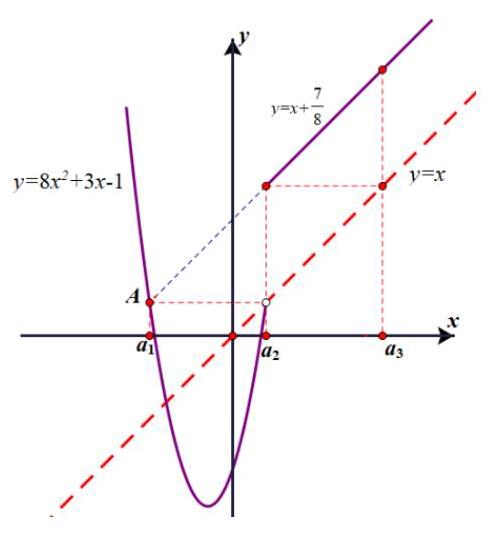
\includegraphics[max width=0.4\textwidth]{images/bo_d6dceus601uc73dvofhg_47_319_223_486_534_0.jpg}
\end{center}
\hspace*{3em} 

图 12-1

\begin{center}
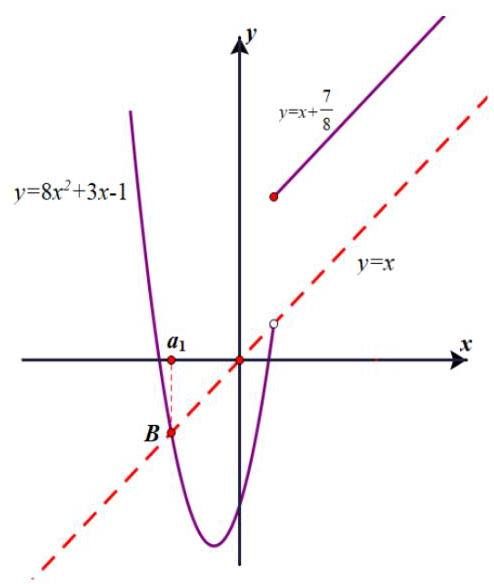
\includegraphics[max width=0.4\textwidth]{images/bo_d6dceus601uc73dvofhg_47_839_184_494_584_0.jpg}
\end{center}
\hspace*{3em} 

图 12-2

依题意可得: 当 \({a}_{1} \geq  \frac{1}{4}\) 时,显然 \(\left\{  {a}_{n}\right\}\) 是等差数列,满足题意;

联立方程 \(\left\{  \begin{array}{l} y = 8{x}^{2} + {3x} - 1 \\  y = x + \frac{7}{8} \end{array}\right.\) ，解得 \({x}_{A} =  - \frac{5}{8}\left( {{x}_{2} = \frac{1}{2}}\right.\) 舍)，如图 12-1，

此时当 \({a}_{1} =  - \frac{5}{8}\) ,则 \(\left\{  {a}_{n}\right\}\) 为等差数列,满足题意;

再联立方程 \(\left\{  \begin{array}{l} y = 8{x}^{2} + {3x} - 1 \\  y = x \end{array}\right.\) ,解得 \({x}_{B} =  - \frac{1}{2}\left( {{x}_{2} = \frac{1}{4}}\right.\) 舍),如图 12-2,

此时当 \({a}_{1} =  - \frac{1}{2}\) ,则 \({a}_{n} =  - \frac{1}{2}\) ,即 \(\left\{  {a}_{n}\right\}\) 也是等差数列,满足题意;

综上所述: 当 \({a}_{1} \in  \left\{  {-\frac{5}{8}, - \frac{1}{2}}\right\}   \cup  \left\lbrack  {\frac{1}{4}, + \infty }\right)\) 时,均可使得 \(\left\{  {a}_{n}\right\}\) 为等差数列. \(\approx\)

2.【 2025.12 崇明高三一模 12】设 \(M = \left\{  {x\left| {\;1 \leq  x \leq  {20}}\right. ,x \in  \mathbf{N}}\right\}\) . 数列 \(\left\{  {a}_{n}\right\}\) 满足下列条件: \({a}_{1} = 1\) , \({a}_{20} = 5,{a}_{k + 1} - {a}_{k} \in  \{ 0,1\}\) ,且对任意的 \(i,j \in  M\) ,都存在 \(m,n \in  M\) 使得 \({a}_{i} + {a}_{j} = {a}_{m} + {a}_{n}\) ,其中 \(i,j,m,n\) 互不相等,则数列 \(\left\{  {a}_{n}\right\}\) 的前 20 项和的最大值是\_\_\_\_\_.

【答案】 74

【解析】由 \({a}_{1} = 1,{a}_{20} = 5,{a}_{k + 1} - {a}_{k} \in  \{ 0,1\}\) 可知: \({a}_{k + 1} - {a}_{k}\) 中,有 4 个差值为 1,

其余 15 个全为 0 . 因此数列 \(\left\{  {a}_{n}\right\}\) 中一定能取遍 \(1 \sim  5\) 中所有的数,且为增数列.

又因为对任意的 \(i,j \in  M\) ,都存在 \(m,n \in  M\) 使得 \({a}_{i} + {a}_{j} = {a}_{m} + {a}_{n}\) ,且 \(i,j,m,n\) 互不相等,所以

\(\left\{  {a}_{n}\right\}\) 中必须至少含有 4 项为 1,也至少含有 4 项为 5 ; 至少含有 2 项为 2; 也至少含有 2 项为 4 ; 至少含有 1 项为 3 .

要使前 20 项和的最大,则剩余的 7 项均为 5,此时 \(\left\{  {a}_{n}\right\}\) 中排列如下: 4 个1,2个2,1个 3,2个4,11个5,此时 \({S}_{20} = 4 \times  1 + 2 \times  2 + 1 \times  3 + 2 \times  4 + {11} \times  5 = {74}\) .

【总结】此题与 2023 届金山一模 12 题如出一辙. \(>  <\)

【附】(2023 届金山模 12)设 \(\left\{  {a}_{n}\right\}\) 是由正整数组成且项数为 \(m\) 的增数列,已知 \({a}_{1} = 1,{a}_{m} = {100}\) , 数列 \(\left\{  {a}_{n}\right\}\) 任意相邻两项的差的绝对值不超过 1,若对于 \(\left\{  {a}_{n}\right\}\) 中任意序数不同的两项 \({a}_{s}\) 和 \({a}_{t}\) , 在剩下的项中总存在序数不同的两项 \({a}_{p}\) 和 \({a}_{q}\) ,使得 \({a}_{s} + {a}_{t} = {a}_{p} + {a}_{q}\) ,则 \(\mathop{\sum }\limits_{{i = 1}}^{m}{a}_{i}\) 的最小值为\_\_\_\_\_.

【答案】 5454

【解析】要求 \(\mathop{\sum }\limits_{{i = 1}}^{m}{a}_{i}\) 的最小值,即项数要尽量少,即相邻两项的差的绝对值尽量为 1 ,

\(\therefore\) 可以先列出等差数列 \(1,2,3\cdots {98},{99},{100}\) .

若任意序数不同的两项 \({a}_{s}\) 和 \({a}_{t}\) 为最小的 1 和 2,那对应的 \({a}_{p}\) 和 \({a}_{q}\) 也要为 1 和 2 ;

同理,若 \({a}_{s}\) 和 \({a}_{t}\) 为最大的 99 和 100,那对应的 \({a}_{p}\) 和 \({a}_{q}\) 也要为 99 和 100,

即数列 \(1,1,2,2,3,4\cdots {97},{98},{99},{99},{100},{100}\) ;

此时若 \({a}_{s}\) 和 \({a}_{t}\) 为最小的 1 和 1 ，则对应的 \({a}_{p}\) 和 \({a}_{q}\) 也要为 1 和 1 ；

同理,若 \({a}_{s}\) 和 \({a}_{t}\) 为最大的 100 和 100,则对应的 \({a}_{p}\) 和 \({a}_{q}\) 也要为 100 和 100,

即数列 \(1,1,1,1,2,2,3,4\cdots {97},{98},{99},{99},{100},{100},{100}\) ,100符合题意,且项数最少,

此时 \(\mathop{\sum }\limits_{{i = 1}}^{m}{a}_{i} = \frac{\left( {1 + {100}}\right)  \times  {100}}{2} + 3 \times  1 + 2 + {99} + 3 \times  {100} = {5454}\) .

3.【 2025.12 杨浦高三一模 12】数列 \(A : {a}_{1},{a}_{2},\cdots ,{a}_{100}\) 满足: \({a}_{i} \in  N\left( {1 \leq  i \leq  {100}}\right)\) ,且 \(1 = {a}_{1} < {a}_{2} < \cdots  < {a}_{100} = {2025}\) ,记集合 \(M\left( A\right)  = \left\{  {\left( {{b}_{1},{b}_{2},\cdots ,{b}_{100}}\right)  \mid  {b}_{1} = 1,{b}_{100} = {2025},{b}_{i} = {a}_{i - 1} + 1}\right.\) 或 \(\left. {{b}_{i} = {a}_{i + 1} - 1,i = 2,3,\cdots ,{99}}\right\}\) 。若数列 \(A\) 满足: 对任意 \(\left( {{b}_{1},{b}_{2},\cdots ,{b}_{100}}\right)  \in  M\left( A\right)\) ,均有 \({b}_{1} < {b}_{2} < \cdots  < {b}_{100}\) , 则称数列 \(A\) 是 “好的 “. ”好的 “数列 \(A\) 的个数为\_\_\_\_\_.

【答案】1926

【解析】依题意可得: 要使 \({b}_{i} < {b}_{i + 1}\) ,则需 \({\left( {b}_{i}\right) }_{\max } < {\left( {b}_{i + 1}\right) }_{\min }\) ,即 \({a}_{i + 1} - 1 < {a}_{i} + 1\) ,也即 \({a}_{i + 1} - {a}_{i} < 2\)

又由于数列 \(\left\{  {a}_{n}\right\}\) 为严格递增数列且 \({a}_{n} \in  \mathbb{N},\therefore {a}_{i + 1} - {a}_{i} \geq  1\) .

所以 \(2 > {a}_{i + 1} - {a}_{i} \geq  1\) ,所以只能是 \({a}_{i + 1} - {a}_{i} = 1\left( {2 \leq  i \leq  {98}}\right)\) .

设 \({a}_{2} = t \in  \mathbb{N}\) ,则 \({a}_{99} = t + {97}\) .

又 \(\because {a}_{1} < {a}_{2} < {a}_{3} < \cdots  < {a}_{99} < {a}_{100},\therefore \left\{  \begin{array}{l} t > 1 \\  t + {97} < {2025} \end{array}\right.\) ,解得 \(1 < t < {1928}\) 且 \(t \in  \mathbb{N}\) .

\(\therefore\) 正整数 \(t\) 的取值可以是 \(2 \sim  {1927}\) ,故符合条件的数量 \(\left\{  {a}_{n}\right\}\) 共有 1296 个.

4.【2025.12 徐汇高三一模 12】已知数列 \(\left\{  {a}_{n}\right\}\) 满足: \({a}_{1} = 0\) ,对任意的正整数 \(n\) 均有 \({a}_{n} - {a}_{n - 1} \in  \{ 1,2\}\) ,若存在正整数 \(k\left( {1 \leq  k \leq  9}\right)\) ,使得所有数列 \(\left\{  {a}_{n}\right\}\) 均满足 \({a}_{1} + {a}_{2} + \cdots  + {a}_{k} \leq  {a}_{k + 1} + {a}_{k + 2} + \cdots  + {a}_{10}\) ，则 \(k\) 的最大值为\_\_\_\_\_.

【答案】 6

【解析】原不等式左边有 \(k\) 项,右边有 \({10} - k\) 项,要使 \(k\) 取到最大值,即左边的项数尽可能多, 右边项数就少, 因此可考虑取极端情况:

当 \(1 \leq  n \leq  k + 1\) 时, \({a}_{n} - {a}_{n - 1} = 2\) ;

当 \(k + 2 \leq  n \leq  {10}\) 时, \({a}_{n} - {a}_{n - 1} = 1\) .

所以当 \(1 \leq  n \leq  k\) 时,累加得 \({a}_{n} = \left( {{a}_{n} - {a}_{n - 1}}\right)  + \left( {{a}_{n - 1} - {a}_{n - 2}}\right)  + \cdots  + \left( {{a}_{2} - {a}_{1}}\right)  + {a}_{1} = 2\left( {n - 1}\right)\) ,

所以 \({a}_{1} + {a}_{2} + \cdots  + {a}_{k} = \frac{\left\lbrack  {0 + 2\left( {k - 1}\right) }\right\rbrack  k}{2} = \left( {k - 1}\right) k\) ;

当 \(k + 1 \leq  n \leq  {10}\) 时,

累加得 \({a}_{n} = \left( {{a}_{n} - {a}_{n - 1}}\right)  + \left( {{a}_{n - 1} - {a}_{n - 2}}\right)  + \cdots  + \left( {{a}_{k + 1} - {a}_{k}}\right)  + {a}_{k} = n - k + 2\left( {k - 1}\right)  = n + k - 2\) .

所以 \({a}_{k + 1} + {a}_{k + 2} + \cdots  + {a}_{10} = \frac{\left\lbrack  {\left( {{2k} - 1}\right)  + \left( {k + 8}\right) }\right\rbrack  \left( {{10} - k}\right) }{2} = \frac{-3{k}^{2} + {23k} + {70}}{2}\) .

由 \({a}_{1} + {a}_{2} + \cdots  + {a}_{k} \leq  {a}_{k + 1} + {a}_{k + 2} + \cdots  + {a}_{10}\) 得 \(\left( {k - 1}\right) k \leq  \frac{-3{k}^{2} + {23k} + {70}}{2}\) ,

解得 \(k \leq  \frac{{23} + \sqrt{1969}}{10} \approx  {6.7}\) ,所以满足条件的 \(k\) 的最大值为 6.9 (   )

5.【2025.12 金山高三一模 15】已知正整数 \({a}_{1}\text{ 、 }{a}_{2}\text{ 、 }{a}_{3}\) ,满足 \(1 \leq  {a}_{1} < {a}_{2} < {a}_{3} \leq  {10}\) ,且 \(\left( {{a}_{1}^{2} + {a}_{2}^{2}}\right) \left( {{a}_{2}^{2} + {a}_{3}^{2}}\right)  = {\left( {a}_{1}{a}_{2} + {a}_{2}{a}_{3}\right) }^{2}\) ,则有序数对 \(\left( {{a}_{1},{a}_{2},{a}_{3}}\right)\) 有(   )个.

A. 5 B. 4 C. 3 D. 2

【答案】B

【解析】由 \(\left( {{a}_{1}^{2} + {a}_{2}^{2}}\right) \left( {{a}_{2}^{2} + {a}_{3}^{2}}\right)  = {\left( {a}_{1}{a}_{2} + {a}_{2}{a}_{3}\right) }^{2}\) 化简得 \({a}_{2}{}^{2} = {a}_{1}{a}_{3}\) .

结合 \(1 \leq  {a}_{1} < {a}_{2} < {a}_{3} \leq  {10}\) 且 \({a}_{1},{a}_{2},{a}_{3}\) 均为正整数,则 \(\left( {{a}_{1},{a}_{2},{a}_{3}}\right)  = \left( {1,2,4}\right)\) 或 \(\left( {1,3,9}\right)\) 或 \(\left( {2,4,8}\right)\) 或 \(\left( {4,6,9}\right)\) ，共 4 个，选 B.C.

6.【2025.12 静安高三一模 15】若数列 \(\left\{  {a}_{n}\right\}\) 满足 \({a}_{n + 1} = {\log }_{m}{a}_{n}\;\left( {m > 1}\right.\) 且 \(m \in  \mathbb{Z},n\) 为正整数),则称数列 \(\left\{  {a}_{n}\right\}\) 为“对数 \(m\) 底数列”. 已知正项数列 \(\left\{  {a}_{n}\right\}\) 是“对数 2 底数列”,且 \({a}_{5} = 1\) , 则当 \(n \geq  2\) 时， \(\frac{{4}^{{a}_{2} + {a}_{3} + \cdots  + {a}_{n}}}{{a}_{2}^{2}\cdots {a}_{n - 1}^{2}} =\) (   ).

A. \({2}^{16}\) B. \({2}^{12}\) C. \({2}^{64}\) D. \({2}^{32}\)

【答案】D

【解析】依题意可得: \({a}_{n + 1} = {\log }_{2}{a}_{n}\) ,由 \({a}_{5} = 1\) 得 \({a}_{4} = 2,{a}_{3} = 4,{a}_{2} = {16}\) .

同时有 \({2}^{{a}_{n + 1}} = {a}_{n}\) ,即 \({2}^{{a}_{n}} = {a}_{n - 1},\therefore {4}^{{a}_{n}} = {a}_{n - 1}{}^{2},{4}^{{a}_{n - 1}} = {a}_{n - 2}{}^{2},\cdots ,{4}^{{a}_{3}} = {a}_{2}{}^{2}\) .

\(\therefore \frac{{4}^{{a}_{2} + {a}_{3} + \cdots  + {a}_{n}}}{{a}_{2}^{2}\cdots {a}_{n - 1}^{2}} = {4}^{{a}_{2}} = {4}^{16} = {2}^{32}\) ,选 D. \(<\)

7.【2025.12 黄浦高三一模 15】若数列 \(\left\{  {a}_{n}\right\}\) 同时满足如下条件:

(i) \(\left\{  {a}_{n}\right\}\) 是无穷数列;

(ii) \(\left\{  {a}_{n}\right\}\) 是严格增数列;

(iii) 存在正数 \(M\) ,使得对任意的 \(n \in  {\mathbb{N}}^{ * }\) ,都有 \(\left\{  {a}_{n}\right\}\) 的前 \(n\) 项的和 \({S}_{n} \in  \left\lbrack  {-M,M}\right\rbrack\) . 则称 \(\left\{  {a}_{n}\right\}\) 具有性质 \(P\) . 关于如下结论: 其中正确的说法是( )

 \circled{1} 存在等差数列具有性质 \(P\) ； \circled{2} 存在等比数列具有性质 \(P\)

A.  \circled{1} 和 \circled{2} 均正确 B.  \circled{1} 和 \circled{2} 均错误

C.  \circled{1} 正确， \circled{2} 错误 D.  \circled{1} 错误， \circled{2} 正确

【答案】D

【解析】对于命题 \circled{1} : 当 \(\left\{  {a}_{n}\right\}\) 为严格递增的等差数列时, \(d > 0\) ,则 \({S}_{n} = \frac{d}{2}{n}^{2} + \left( {{a}_{1} - \frac{d}{2}}\right) n\)

表示一个关于 \(n\) 的二次函数,开口朝上. 当 \(n \rightarrow   + \infty\) 时, \({S}_{n} \rightarrow   + \infty\) ,此时不可能存在正数 \(M\) 满足 \({S}_{n} \in  \left\lbrack  {-M,M}\right\rbrack\) ,故 \circled{1} 为假命题;

对于命题 \circled{2} :当 \(\left\{  {a}_{n}\right\}\) 为严格递增的等比数列时，显然 \(q > 0\) 且 \(q \neq  1\) .

若 \({a}_{1} > 0\) ,则 \(q > 1\) ,此时 \({S}_{n} = \frac{{a}_{1}\left( {1 - {q}^{n}}\right) }{1 - q}\) . 当 \(n \rightarrow   + \infty\) 时, \({S}_{n} \rightarrow   + \infty\) ,此时不可能存在正数 \(M\)

满足 \({S}_{n} \in  \left\lbrack  {-M,M}\right\rbrack\) ;

若 \({a}_{1} < 0\) ,则 \(1 > q > 0\) ,此时 \({S}_{n} = \frac{{a}_{1}\left( {1 - {q}^{n}}\right) }{1 - q}\) 单调递减. 当 \(n \rightarrow   + \infty\) 时, \({S}_{n} \rightarrow  \frac{{a}_{1}}{1 - q}\) ,此时只需正数 \(M\) 满足 \(M \geq  \left| \frac{{a}_{1}}{1 - q}\right|\) 即可,故此时 \circled{2} 命题为真命题. \(>\)

8.【2025.12 普陀高三一模 16】设 \(n \geq  1,n \in  \mathbf{N}\) ，数列 \(\left\{  {a}_{n}\right\}\) 和 \(\left\{  {b}_{n}\right\}\) 满足 \({a}_{1} = {b}_{1} = 1\) ，且 \({a}_{n + 1} \in  \{ 0,1\} ,{b}_{n + 1} = \left| {{a}_{n + 1} - 2{a}_{n}}\right| {b}_{n}\) ,现有如下两个命题:

 \circled{1} 若数列 \(\left\{  {b}_{n}\right\}\) 是等比数列，则数列 \(\left\{  {a}_{n}\right\}\) 是常数列;

 \circled{2}  设 \({S}_{n}\) 是数列 \(\left\{  {b}_{n}\right\}\) 的前 \(n\) 项和，若 \({b}_{2026}\) 取得最大值时，则 \({S}_{2026} - 2\) 能被 7 整除.

则下列结论中正确的是( ).

A.  \circled{1} 为真 \circled{2} 为真 B.  \circled{1} 为真 \circled{2} 为假 C.  \circled{1} 为假 \circled{2} 为真 D.  \circled{1} 为假 \circled{2} 为

假

【答案】A

【解析】对命题 \circled{1} :

由 \({b}_{n + 1} = \left| {{a}_{n + 1} - 2{a}_{n}}\right|  \cdot  {b}_{n}\) 得 \({b}_{2} = \left| {{a}_{2} - 2{a}_{1}}\right|  \cdot  {b}_{1} = \left| {{a}_{2} - 2}\right|  \cdot  {b}_{1}\) ,则 \({a}_{2} - 2 =  - 2\) 或-1.

当 \(\left\{  {b}_{n}\right\}\) 为等比数列,则若 \({a}_{2} - 2 =  - 2\) 时,此时 \({b}_{2} = 2{b}_{1}\) ,公比为 2,则 \(\left| {{a}_{n + 1} - 2{a}_{n}}\right|  = 2\) ,

此时无论是 \({a}_{n + 1} - 2{a}_{n} = 2\) 还是 \({a}_{n + 1} - 2{a}_{n} =  - 2\) ,都与 \({a}_{n + 1} \in  \{ 0,1\}\) 矛盾,均不符;

所以当 \(\left\{  {b}_{n}\right\}\) 为等比数列,只能是 \({a}_{2} - 2 =  - 1\) ,此时 \({b}_{2} = {b}_{1}\) ,公比为 1,即 \(\left| {{a}_{n + 1} - 2{a}_{n}}\right|  = 1\) .

若 \({a}_{n + 1} - 2{a}_{n} = 1\) ,则可得 \({a}_{n + 1} + 1 = 2\left( {{a}_{n} + 1}\right)\) ,这仍与 \({a}_{n + 1} \in  \{ 0,1\}\) 矛盾,不符;

若 \({a}_{n + 1} - 2{a}_{n} =  - 1\) ,则可得 \({a}_{n + 1} - 1 = 2\left( {{a}_{n} - 1}\right)\) ,结合 \({a}_{n + 1} \in  \{ 0,1\}\) ,只能是 \({a}_{n + 1} = 1\) ,此时 \(\left\{  {a}_{n}\right\}\)

为常数列; \(\therefore\)  \circled{1} 命题为真命题；

对命题 \circled{2} :

由 \circled{1} 可知: \(\left| {{a}_{2} - 2{a}_{1}}\right|  = 2\) 或 1，要使 \({b}_{2026}\) 尽可能大，则 \(\left| {{a}_{2} - 2{a}_{1}}\right|  = 2\) ，解得 \({a}_{2} = 0\) ；

则 \(\left| {{a}_{3} - 2{a}_{2}}\right|  = \left| {a}_{3}\right|  = 1\) 或 0, \(\therefore\) 得取 \({a}_{3} = 1;\left| {{a}_{4} - 2{a}_{3}}\right|  = \left| {{a}_{4} - 2}\right|  = 2\) 或 1,得取 \({a}_{4} = 0;\ldots\)

以此类推,可得 \({a}_{n} = \left\{  {\begin{array}{ll} 1 & n = {2k} - 1 \\  0 & n = {2k} \end{array}\left( {k \in  \mathbb{N},k \geq  1}\right) }\right.\) ,

此时 \({b}_{n + 1} = \left| {{a}_{n + 1} - 2{a}_{n}}\right|  \cdot  {b}_{n} = \left\{  {\begin{array}{ll} 2{b}_{n} & n = {2k} - 1 \\  {b}_{n} & n = {2k} \end{array}\left( {k \in  \mathbb{N},k \geq  1}\right) }\right.\) ,

\(\therefore {b}_{n} = \left\{  {\begin{array}{ll} {2}^{\frac{n - 1}{2}} & n = {2k} - 1 \\  {2}^{\frac{n}{2}} & n = {2k} \end{array}\left( {k \in  \mathbb{N},k \geq  1}\right) .}\right.\)

\(\therefore {S}_{2026} = \left( {{b}_{1} + {b}_{3} + \cdots  + {b}_{2025}}\right)  + \left( {{b}_{2} + {b}_{4} + \cdots  + {b}_{2026}}\right)  = 3\left( {{b}_{1} + {b}_{3} + \cdots  + {b}_{2025}}\right)\)

\(= 3 \times  \frac{1 - {2}^{1013}}{1 - 2} = 3\left( {{2}^{1013} - 1}\right)\) .

其中 \({2}^{1013} = 4 \times  {\left( {2}^{3}\right) }^{337} = 4{\left( 7 + 1\right) }^{337} = 4\left( {{C}_{337}^{0}{7}^{337} + {C}_{337}^{1}{7}^{336} + \cdots  + {C}_{337}^{336}{7}^{1} + {C}_{337}^{337}{7}^{0}}\right)\) ,被 7 除余 4, 因此 \({S}_{2026} - 2 = 3 \times  {2}^{1013} - 5\) 被 7 整除,故 \circled{2} 也为真命题

9.【2025.12 嘉定高三一模 16】数列 \(\left\{  {a}_{n}\right\}\) 的前 \(n\) 项和为 \({S}_{n}\) ，且对任意正整数 \(n\) ，总存在正整数 \(m\) ,使得 \({S}_{n} = {a}_{m}\) . 则下列命题中正确的是 ( )

A. 对任意正整数 \(n\) ,总存在正整数 \(m\) ,使得 \({a}_{n} = {S}_{m}\)

B. 数列 \(\left\{  {a}_{n}\right\}\) 一定是等差数列

C. 存在公比为正整数的等比数列 \(\left\{  {a}_{n}\right\}\) 满足条件

D. 对任意正整数 \(k\) ,总存在正整数 \(m,n\) ,使得 \({a}_{k} = {a}_{m} - {a}_{n}\)

【答案】D

【解析】因为对任意正整数 \(n\) ,总存在正整数 \(m\) ,使得 \({S}_{n} = {a}_{m}\) ,

所以当 \(k = 1\) 时,存在正整数 \(m\) 满足 \({S}_{2} = {a}_{m} = {a}_{1} + {a}_{2}\) ,即 \({a}_{1} = {a}_{m} - {a}_{2}\) ,满足题意;

当 \(k \geq  2\) 时, \({S}_{k} = {a}_{m},{S}_{k - 1} = {a}_{n}\) ,作差得 \({a}_{k} = {a}_{m} - {a}_{n}\) ,也满足题意,故 \(\mathrm{D}\) 正确.

现说明其它几个选项:

选项 A: 若 \(\left\{  {a}_{n}\right\}\) 为等差数列且通项为 \({a}_{n} = n\) ,则 \({S}_{n} = \frac{n\left( {n + 1}\right) }{2}\) . 当 \(n = 2\) 时,不存在这样的正整数 \(m\) 使得 \({a}_{n} = {S}_{m}\) , A 错误;

选项 B:若 \(\left\{  {a}_{n}\right\}\) 的通项公式为 \({a}_{n} = \left\{  \begin{array}{ll} 0 & n = 1 \\  n - 2 & n \geq  2 \end{array}\right.\) ，则 \({S}_{n} = \left\{  \begin{array}{ll} 0 & n = 1 \\  \frac{\left( {n - 2}\right) \left( {n - 1}\right) }{2} & n \geq  2 \end{array}\right.\) ，满足题意,但此时 \(\left\{  {a}_{n}\right\}\) 并非等差数列, B 错误;

选项 C: 若 \(\left\{  {a}_{n}\right\}\) 为等比数列,公比 \(q\) 为正整数,显然 \(q = 1\) 时不符题意,则 \(q \geq  2\) ,此时由 \({S}_{n} = {a}_{m}\) 得 \({a}_{1}\left( {1 + q + {q}^{2} + \cdots  + {q}^{n - 1}}\right)  = {a}_{1} \cdot  {q}^{m - 1},\therefore 1 + q + {q}^{2} + \cdots  + {q}^{n - 1} = {q}^{m - 1}\) .

\(\because q \geq  2,\therefore m > n\) ,故 \(m - 1 \geq  n\) .

再由 \({S}_{n} = {a}_{m}\) 得 \(\frac{{a}_{1}\left( {1 - {q}^{n}}\right) }{1 - q} = {a}_{1} \cdot  {q}^{m - 1}\) ,化简得 \({q}^{n} - 1 = {q}^{m - 1}\left( {q - 1}\right)\) ,故 \(1 - \frac{1}{{q}^{n}} = {q}^{m - n - 1}\left( {q - 1}\right)\) .

\(\because q \geq  2\) 且 \(q \in  \mathbb{N}\) ， \(\therefore\) 左边 \(1 - \frac{1}{{q}^{n}} < 1\) ，右边 \({q}^{m - n - 1}\left( {q - 1}\right)  \in  {\mathbb{N}}^{ * }\) ，上式显然不可能成立，故不存在公比为正整数的等比数列 \(\left\{  {a}_{n}\right\}\) 满足条件, C 错误。

10.【2025.12 虹口高三一模 16】若每一项均为正数的数列 \(\left\{  {a}_{n}\right\}\) 的前 \(n\) 项和为 \({S}_{n}\) ，且对于任意的正整数 \(n\) ,均存在正整数 \(m\) 使得 \(\frac{{a}_{n} - {S}_{m}}{{a}_{n} - {S}_{m + 1}} \leq  0\) ,则称 \(\left\{  {a}_{n}\right\}\) 具有“ \(P\) 性质”. 对于以下命题, 说法正确的是( )

 \circled{1}  存在等比数列 \(\left\{  {a}_{n}\right\}\) ，使得 \(\left\{  {a}_{n}\right\}\) 具有“ \(P\) 性质”;

 \circled{2}  若 \(\left\{  {a}_{n}\right\}\) 具有“ \(P\) 性质”，记 \({\Delta }_{n} = {S}_{m + 1} - {a}_{n}\) 且 \(\left\{  {\Delta }_{n}\right\}\) 为等差数列，则 \({S}_{n} \leq  {2}^{n} \cdot  {a}_{1}\) .

A.  \circled{1} 和 \circled{2} 都为真命题 B.  \circled{1} 和 \circled{2} 都为假命题

C.  \circled{1} 为真命题， \circled{2} 为假命题 D.  \circled{1} 为假命题， \circled{2} 为真命题

【答案】A

【解析】若 \(\left\{  {a}_{n}\right\}\) 具有“ \(P\) 性质”,且每一项均为正数,则 \({S}_{m + 1} > {S}_{m}\) .

由 \(\frac{{a}_{n} - {S}_{m}}{{a}_{n} - {S}_{m + 1}} \leq  0\) 可得 \({S}_{m} \leq  {a}_{n} < {S}_{m + 1}\) .

命题 \circled{1} :若等比数列 \(\left\{  {a}_{n}\right\}\) 为常值数列，比如 \({a}_{n} = 1\) ，则 \({S}_{1} = 1,{S}_{2} = 2\) ，则对任意的正整数 \(n\) ， 均有 \({a}_{n} \in  \left\lbrack  {{S}_{1},{S}_{2}}\right)\) 满足题意,故此时 \(\left\{  {a}_{n}\right\}\) 具有“ \(P\) 性质”, \circled{1} 为真命题;

命题 \circled{2} :若 \(\left\{  {a}_{n}\right\}\) 具有“ \(P\) 性质”，则 \({S}_{1} \leq  {a}_{1} < {S}_{2}\) ，又由 \({a}_{n} > 0\) 得 \({S}_{1} \leq  {a}_{2} < {S}_{2}\) ， \(\therefore {a}_{1} \leq  {a}_{2}\) .

由 \(\left\{  {\Delta }_{n}\right\}\) 为等差数列得 \({\Delta }_{n} = {S}_{m + 1} - {a}_{n} > 0,\therefore \left\{  {\Delta }_{n}\right\}\) 每项均为正值， \(\therefore d \geq  0\) .

再由 \({\Delta }_{n} = {S}_{m + 1} - {a}_{n}\) 得 \({\Delta }_{1} = {S}_{2} - {a}_{1},{\Delta }_{2} = {S}_{2} - {a}_{2}\) ,

\(\therefore d = {\Delta }_{2} - {\Delta }_{1} = \left( {{S}_{2} - {a}_{2}}\right)  - \left( {{S}_{2} - {a}_{1}}\right)  = {a}_{1} - {a}_{2} \geq  0\) ,即 \({a}_{1} \geq  {a}_{2}\) ,所以只有 \({a}_{1} = {a}_{2}\) ,故 \(d = 0,\therefore \; {\Delta }_{n} = {S}_{m + 1} - {a}_{n} = {a}_{1},\therefore {\Delta }_{3} = {S}_{m + 1} - {a}_{3} = {a}_{1},\)

从而 \({S}_{m + 1} = {a}_{1} + {a}_{3} > {a}_{3} \geq  {S}_{m},\therefore {S}_{m + 1} = {S}_{2},{S}_{m} = {S}_{1}\) ,从而 \({a}_{3} = {a}_{2} = {a}_{1}\) ;

\({\Delta }_{4} = {S}_{m + 1} - {a}_{4} = {a}_{1},\;{a}_{1} + {a}_{2} \leq  {a}_{4} < {S}_{m + 1} = {a}_{1} + {a}_{4} < {S}_{4},\)

从而 \({a}_{4} \leq  {a}_{2} + {a}_{3} = 2{a}_{1};{a}_{5} \leq  {a}_{2} + {a}_{3} + {a}_{4} \leq  {2}^{2} \cdot  {a}_{1};{a}_{6} \leq  {a}_{2} + {a}_{3} + {a}_{4} + {a}_{5} \leq  {2}^{3} \cdot  {a}_{1}\) ;

以此类推, \({S}_{n} = {a}_{1} + {a}_{2} + {a}_{3} + \cdots  + {a}_{n} \leq  3{a}_{1} + \left( {{2}^{1} + {2}^{2} + \cdots  + {2}^{n - 3}}\right)  = \left( {{2}^{n - 2} + 1}\right)  \cdot  {a}_{1} \leq  {2}^{n} \cdot  {a}_{1}\) ,得证,

\(\therefore\) 命题 \circled{2} 为真命题. \(\approx\)

11.【2025.12 长宁高三一模 16】将正整数 1\textasciitilde 10 按一定次序排列得到数列 \({a}_{1},{a}_{2},\cdots ,{a}_{10}\) . 若数列 \({a}_{1},{a}_{2},\cdots ,{a}_{10}\) 中的任意一项 \({a}_{i}\left( {1 \leq  i \leq  {10}}\right)\) 都满足: \(- 1 \leq  {a}_{i} - i \leq  1\) ,则数列 \({a}_{1},{a}_{2},\cdots ,{a}_{10}\) 的个数为 ( ) .

A. 36; B.55; C. 89; D.144.

【答案】C

【解析】设 \(1 \sim  n\) 时,满足条件的数列个数为 \(f\left( n\right)\) ,显然 \(f\left( 1\right)  = 1,f\left( 2\right)  = 2\) ;

下面考虑 \(1 \sim  n + 1\) 时,考虑到 \(- 1 \leq  {a}_{n + 1} - \left( {n + 1}\right)  \leq  1\) ,得 \(n \leq  {a}_{n + 1} \leq  n + 2\) ,则 \({a}_{n + 1} = n\) 或 \(n + 1\) . 若 \({a}_{n + 1} = n + 1\) ,此时有 \(f\left( n\right)\) 个;

若 \({a}_{n + 1} = n\) ,则前面 \({a}_{1} \sim  {a}_{n - 1}\) 的次序不变,有 \(f\left( {n - 1}\right)\) 个, \({a}_{n},{a}_{n + 1}\) 的取值也唯一,

只能是 \({a}_{n} = n + 1,{a}_{n + 1} = n\) ,所以此时有 \(f\left( {n - 1}\right)\) 个.

因此 \(f\left( {n + 1}\right)  = f\left( n\right)  + f\left( {n - 1}\right)\) ,故数列 \(f\left( n\right)\) 为“斐波拉契数列”.

\(f\left( 1\right)  = 1;\;f\left( 2\right)  = 2;\;f\left( 3\right)  = 3;\;f\left( 4\right)  = 5;\;f\left( 5\right)  = 8;\;f\left( 6\right)  = {13};\;f\left( 7\right)  = {21};\)

\(f\left( 8\right)  = {34}\) ；

\(f\left( 9\right)  = {55};\;f\left( {10}\right)  = {89}\) ；故选 C. 2 已知

\section*{第六章 向量}

【必背知识点 1】 \circled{1}  向量 \(\overrightarrow{a}\) 与向量 \(\overrightarrow{b}\) 夹角为锐角 \(\Leftrightarrow\) 且 \(\overrightarrow{a}\) 不平行于 \(\overrightarrow{b}\)

 \circled{2}  向量 \(\overrightarrow{a}\) 与向量 \(\overrightarrow{b}\) 夹角为钝角 \(\Leftrightarrow  \overrightarrow{a} \cdot  \overrightarrow{b} < 0\) 且 \(\overrightarrow{a}\) 不平行于 \(\overrightarrow{b}\)

【必背知识点 2】设 \(\overrightarrow{a} = \left( {{x}_{1},{y}_{1}}\right) ,\overrightarrow{b} = \left( {{x}_{2},{y}_{2}}\right)\) ,则 \(\cos \langle \overrightarrow{a},\overrightarrow{b}\rangle  = \frac{\overrightarrow{a} \cdot  \overrightarrow{b}}{\left| \overrightarrow{a}\right| \left| \overrightarrow{b}\right| } = \frac{{x}_{1}{x}_{2} + {y}_{1}{y}_{2}}{\sqrt{{x}_{1}^{2} + {y}_{1}^{2}}\sqrt{{x}_{2}^{2} + {y}_{2}^{2}}}\) .

\(\overrightarrow{a}//\overrightarrow{b} \Leftrightarrow  \overrightarrow{a} = \lambda \overrightarrow{b} \Leftrightarrow  {x}_{1}{y}_{2} - {x}_{2}{y}_{1} = 0 \Leftrightarrow  \overrightarrow{a} \cdot  \overrightarrow{b} =  \pm  \left| \overrightarrow{a}\right| \left| \overrightarrow{b}\right|\)

\(\overrightarrow{a} \bot  \overrightarrow{b} \Leftrightarrow  \overrightarrow{a} \cdot  \overrightarrow{b} = 0 \Leftrightarrow  {x}_{1}{x}_{2} + {y}_{1}{y}_{2} = 0 \Leftrightarrow  \left| {\overrightarrow{a} + \overrightarrow{b}}\right|  = \left| {\overrightarrow{a} - \overrightarrow{b}}\right|\)

【必背知识点 3】向量的投影与数量积

(1)向量的夹角:向量 \(\overrightarrow{a}\) 与 \(\overrightarrow{b}\) 的夹角记为 \(\langle \overrightarrow{a},\overrightarrow{b}\rangle\) ，其值 \(0 \leq  \langle \overrightarrow{a},\overrightarrow{b}\rangle  \leq  \pi\) . \(\overrightarrow{a} \cdot  \overrightarrow{b} > 0\)

(2)向量的投影:向量 \(\overrightarrow{b}\) 在非零向量 \(\overrightarrow{a}\) 方向上的投影是如下的向量: \(\left| \overrightarrow{b}\right| \cos \langle \overrightarrow{a},\overrightarrow{b}\rangle \frac{\overrightarrow{a}}{\left| \overrightarrow{a}\right| }\)

其中，系数 \(\left| \overrightarrow{b}\right| \cos \langle \overrightarrow{a},\overrightarrow{b}\rangle\) 称为向量 \(\overrightarrow{b}\) 在向量 \(\overrightarrow{a}\) 方向上的数量投影.

(3)向量 \(\overrightarrow{a}\) 与 \(\overrightarrow{b}\) 的数量积定义为: \(\overrightarrow{a} \cdot  \overrightarrow{b} = \left| \overrightarrow{a}\right| \left| \overrightarrow{b}\right| \cos \langle \overrightarrow{a},\overrightarrow{b}\rangle\)

【必背知识点 4】平面向量基本定理:给定平面上两个不平行的向量,则该平面内的任意向量都可以唯一地表示为这两个向量的线性组合, 也就是说,平面上任意两个不平行的向量都组成了一组基.

【知识点 5】定比分点公式: \({P}_{1}\left( {{x}_{1},{y}_{1}}\right) ,{P}_{2}\left( {{x}_{2},{y}_{2}}\right) ,\overrightarrow{{P}_{1}P} = \lambda \overrightarrow{P{P}_{2}}\) ,则 \(\mathrm{P}\) 坐标为 \(\left( {\frac{{x}_{1} + \lambda {x}_{2}}{1 + \lambda },\frac{{y}_{1} + \lambda {y}_{2}}{1 + \lambda }}\right)\) 。

【知识点 6】 \(\bigtriangleup {ABC}\) 顶点 \(A\left( {{x}_{1},{y}_{1}}\right) ,B\left( {{x}_{2},{y}_{2}}\right) ,C\left( {{x}_{3},{y}_{3}}\right)\) ，则 \(\bigtriangleup {ABC}\) 重心坐标为 \(\left( {\frac{{x}_{1} + {x}_{2} + {x}_{3}}{3},\frac{{y}_{1} + {y}_{2} + {y}_{3}}{3}}\right)\) 。

【知识点 7】三角形四心定义: 内心: 三角形角平分线的交点; 外心: 三角形中垂线的交点;

重心:三角形中线的交点; 垂心:三角形高的交点; 三角形四“心”向量形式的充要条件: 设 \(\mathrm{O}\) 为 \(\bigtriangleup {ABC}\) 所在平面上一点, \(a,b,c\) 是 \(A,B,C\) 对应的边。

(1)O 为 \({\Delta ABC}\) 的外心 \(\Leftrightarrow  {\overrightarrow{OA}}^{2} = {\overrightarrow{OB}}^{2} = {\overrightarrow{OC}}^{2}\)

(2)O 为 \(\bigtriangleup {ABC}\) 的重心 \(\Leftrightarrow  \overrightarrow{OA} + \overrightarrow{OB} + \overrightarrow{OC} = \overrightarrow{0}\)

(3) \(\mathrm{O}\) 为 \(\bigtriangleup {ABC}\) 的垂心 \(\Leftrightarrow  \overrightarrow{OA} \cdot  \overrightarrow{OB} = \overrightarrow{OB} \cdot  \overrightarrow{OC} = \overrightarrow{OA} \cdot  \overrightarrow{OC}\)

(4) \(\overrightarrow{AP} = \lambda \left( {\frac{\overrightarrow{AB}}{\left| \overrightarrow{AB}\right| } + \frac{\overrightarrow{AC}}{\left| \overrightarrow{AC}\right| }}\right) \left( {\lambda  \in  R}\right)\) ，则 \(\mathrm{P}\) 的轨迹过三角形的内心

\section*{6.1 向量位置关系}

1.【 2025.12 杨浦高三一模 3】已知向量 \(\overrightarrow{a} = \left( {2,3}\right) ,\overrightarrow{b} = \left( {3,x}\right)\) ，且 \(\overrightarrow{a}\bot \overrightarrow{b}\) ，则实数 \(x =\) \_\_\_\_\_.

【答案】-2

【解析】由 \(\overrightarrow{a} \bot  \overrightarrow{b}\) 得 \(\overrightarrow{a} \cdot  \overrightarrow{b} = 6 + {3x} = 0,\therefore x =  - 2\) .

2.【2025.12 浦东高三一模 3】已知向量 \(\overrightarrow{a} = \left( {1, - 3}\right)\) 、 \(\overrightarrow{b} = \left( {1,k}\right)\) ，若 \(\overrightarrow{a}//\overrightarrow{b}\) ，则实数 \(k\) 的值为\_\_\_\_\_.

【答案】 \(k =  - 3\)

【解析】由 \(\overrightarrow{a}//\overrightarrow{b}\) 得 \(\frac{1}{1} = \frac{-3}{k},\therefore k =  - 3\) . \(>  <\)

3.【2025.12 松江高三一模 9】已知平面内两个非零向量 \(\overrightarrow{a},\overrightarrow{b}\) 相互垂直， \(\left| \overrightarrow{a}\right|  = 2\left| \overrightarrow{b}\right|\) ，若 \(\cos \langle \overrightarrow{a} - k\overrightarrow{b},\overrightarrow{b}\rangle  = \frac{\sqrt{2}}{2}\) ,则实数 \(k =\) \_\_\_\_\_.

【答案】 \(k =  - 2\)

【解析】设 \(\overrightarrow{OA} = \overrightarrow{a},\overrightarrow{OB} = \overrightarrow{b}\) ,建系,设 \(A\left( {{2t},0}\right) ,B\left( {0,t}\right)\) (不妨设 \(t > 0\) ).

则 \(\overrightarrow{a} - k\overrightarrow{b} = \overrightarrow{OA} - k\overrightarrow{OB} = \left( {{2t}, - {kt}}\right)\) ,由 \(\cos \langle \overrightarrow{a} - k\overrightarrow{b},\overrightarrow{b}\rangle  = \frac{\sqrt{2}}{2}\) 得 \(\frac{-k{t}^{2}}{\sqrt{{\left( 2t\right) }^{2} + {\left( -kt\right) }^{2}}} = \frac{\sqrt{2}}{2}\) ,

解得 \(k =  - 2\) .

\section*{6.2 投影与数量投影}

1.【2025.12 徐汇高三一模 5】设向量 \(\overrightarrow{a} = \left( {-1, - 2}\right) ,\overrightarrow{b} = \left( {-3,4}\right)\) ,则 \(\overrightarrow{a}\) 在 \(\overrightarrow{b}\) 上的数量投影为\_\_\_\_\_.

【答案】 \(\overrightarrow{a}\) 在 \(\overrightarrow{b}\) 方向上的数量投影为 \(\left| \overrightarrow{a}\right| \cos \langle \overrightarrow{a},\overrightarrow{b}\rangle  = \left| \overrightarrow{a}\right|  \cdot  \frac{\overrightarrow{a} \cdot  \overrightarrow{b}}{\left| \overrightarrow{a}\right|  \cdot  \left| \overrightarrow{b}\right| } =  - 1\) 。

2.【 2025.12 长宁高三一模 6】设 \(\overrightarrow{a} = \left( {2,3}\right) ,\overrightarrow{b} = \left( {1,0}\right)\) ,则向量 \(\overrightarrow{a}\) 在 \(\overrightarrow{b}\) 方向上的投影向量的坐标为\_\_\_\_\_.

【答案】 \(\overrightarrow{a}\) 在 \(\overrightarrow{b}\) 方向上的投影向量为 \(\left| \overrightarrow{a}\right| \cos \langle \overrightarrow{a},\overrightarrow{b}\rangle  \cdot  \frac{\overrightarrow{b}}{\left| \overrightarrow{b}\right| } = \left| \overrightarrow{a}\right|  \cdot  \frac{\overrightarrow{a} \cdot  \overrightarrow{b}}{\left| \overrightarrow{a}\right|  \cdot  \left| \overrightarrow{b}\right| } \cdot  \frac{\overrightarrow{b}}{\left| \overrightarrow{b}\right| } = \frac{\overrightarrow{a} \cdot  \overrightarrow{b}}{\left| \overrightarrow{b}\right| } \cdot  \frac{\overrightarrow{b}}{\left| \overrightarrow{b}\right| } = \left( {2,0}\right)\) . \(\ll\)

3. 【2025.12 虹口高三一模 12】已知空间中四个单位向量 \(\overrightarrow{a},\overrightarrow{b},\overrightarrow{c},\overrightarrow{d}\) 满足 \(\left| {\overrightarrow{a} - \overrightarrow{b}}\right|  = \left| {\overrightarrow{c} - \overrightarrow{d}}\right|  = \left| {\overrightarrow{a} + \overrightarrow{b} + \overrightarrow{c} + \overrightarrow{d}}\right|  = 1\) ，则 \(\overrightarrow{a}\) 在 \(\overrightarrow{c}\) 方向上的数量投影的最大值为\_\_\_\_\_.

【答案】 \(\frac{\sqrt{33} - 5}{12}\)

【解析】为方便表示,设 \(\overrightarrow{a} = \overrightarrow{OA},\overrightarrow{b} = \overrightarrow{OB},\overrightarrow{c} = \overrightarrow{OC},\overrightarrow{d} = \overrightarrow{OD}\) .

由四个单位向量 \(\overrightarrow{a},\overrightarrow{b},\overrightarrow{c},\overrightarrow{d}\) 满足 \(\left| {\overrightarrow{a} - \overrightarrow{b}}\right|  = \left| {\overrightarrow{c} - \overrightarrow{d}}\right|  = 1\) 可知: \(\left| \overrightarrow{AB}\right|  = \left| \overrightarrow{CD}\right|  = 1\) ,

\(\therefore \bigtriangleup {OAB},\bigtriangleup {OCD}\) 均为等边三角形,即 \(\angle {AOB} = \angle {COD} = {60}^{ \circ  },\therefore \left| {\overrightarrow{a} + \overrightarrow{b}}\right|  = \left| {\overrightarrow{c} + \overrightarrow{d}}\right|  = \sqrt{3}\) .

记 \(\overrightarrow{a} + \overrightarrow{b} = \overrightarrow{OM},\overrightarrow{c} + \overrightarrow{d} = \overrightarrow{ON}\) ,即 \(\left| \overrightarrow{OM}\right|  = \left| \overrightarrow{ON}\right|  = \sqrt{3}\) .

再由 \(\left| {\overrightarrow{a} + \overrightarrow{b} + \overrightarrow{c} + \overrightarrow{d}}\right|  = 1\) 得 \(\left| {\overrightarrow{OM} + \overrightarrow{ON}}\right|  = \left| \overrightarrow{OG}\right|  = 1\) ,可得 \(\cos \angle {MON} =  - \frac{5}{6},\sin \angle {MON} = \frac{\sqrt{11}}{6}\) .

\begin{center}
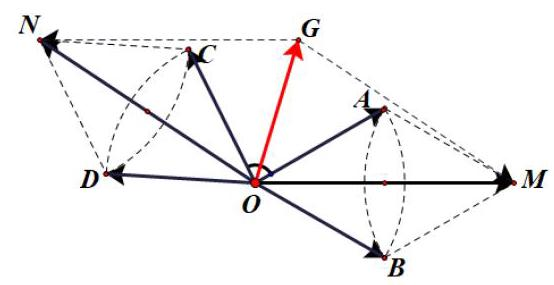
\includegraphics[max width=0.4\textwidth]{images/bo_d6dceus601uc73dvofhg_57_844_899_554_285_0.jpg}
\end{center}
\hspace*{3em} 

如图所示: 当 \(\overrightarrow{OA},\overrightarrow{OC},\overrightarrow{OG}\) 共面时,即 \(\angle {AOC} = \angle {MON} - {60}^{ \circ  }\) 时, \(\overrightarrow{OA}\) 余 \(\overrightarrow{OC}\) 夹角最小,则数量投影最大,此时 \(\cos \angle {AOC} = \cos \left( {\angle {MON} - {60}^{ \circ  }}\right)  = \frac{\sqrt{33} - 5}{12}\) . \(\gg   <\)

6.3 最值

1.【2025.12 闵行高三一模 9】若点 \(P\) 是边长为 1 的正三角形 \({ABC}\) 外接圆上的一点，则 \(\overrightarrow{PA} \cdot  \overrightarrow{BC}\) 的最大值为\_\_\_\_\_.

【答案】 \(\frac{\sqrt{3}}{3}\)

【解析】法 1: 依题意可得: 外接圆半径为 \(R = \frac{\sqrt{3}}{3}\) ,由图可知: \(\overrightarrow{PA}\) 在 \(\overrightarrow{BC}\) 方向上的数量投影最大为 \(R = \frac{\sqrt{3}}{3},\therefore {\left( \overrightarrow{PA} \cdot  \overrightarrow{BC}\right) }_{\max } = \frac{\sqrt{3}}{3} \cdot  1 = \frac{\sqrt{3}}{3}\) .

法 2: 如图所示: 以 \(O\) 为原点建立平面直角坐标系:

\(O\left( {0,0}\right) ,A\left( {0,\frac{\sqrt{3}}{3}}\right) ,B\left( {-\frac{1}{2}, - \frac{\sqrt{3}}{6}}\right) ,C\left( {\frac{1}{2}, - \frac{\sqrt{3}}{6}}\right) ,P\left( {\frac{\sqrt{3}}{3}\cos \theta ,\frac{\sqrt{3}}{3}\sin \theta }\right)\) ,

\(\overrightarrow{PA} = \left( {-\frac{\sqrt{3}}{3}\cos \theta ,\frac{\sqrt{3}}{3} - \frac{\sqrt{3}}{3}\sin \theta }\right) ,\overrightarrow{BC} = \left( {1,0}\right)\) ,所以 \(\overrightarrow{PA} \cdot  \overrightarrow{BC} =  - \frac{\sqrt{3}}{3}\cos \theta\) ,

所以当 \(\cos \theta  =  - 1\) 时， \({\left( \overrightarrow{PA} \cdot  \overrightarrow{BC}\right) }_{\max } = \frac{\sqrt{3}}{3}\)

\begin{center}
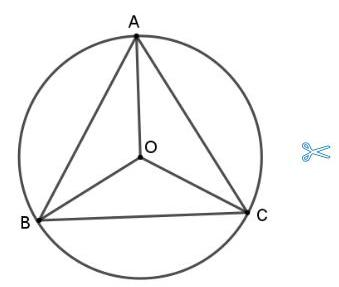
\includegraphics[max width=0.2\textwidth]{images/bo_d6dceus601uc73dvofhg_58_1072_418_339_287_0.jpg}
\end{center}
\hspace*{3em} 

2.【2025.12 金山高三一模 10】已知非零向量 \(\overrightarrow{a}\) 、 \(\overrightarrow{b}\) 的夹角为 \(\theta\) ，若 \(\frac{\left| \overrightarrow{b}\right| }{\left| \overrightarrow{a}\right| } = \cos \theta\) ， \(\left| {\overrightarrow{a} - \overrightarrow{b}}\right|  = 3\) ， 则 \(\left| {\overrightarrow{a} - t\overrightarrow{b}}\right| \left( {t \in  \mathbf{R}}\right)\) 的最小值为\_\_\_\_\_.

【答案】 3

【解析】依题意可设 \(\overrightarrow{a} = \overrightarrow{OA},\overrightarrow{b} = \overrightarrow{OB}\) ,再设 \(t\overrightarrow{b} = \overrightarrow{OC}\) ,则点 \(C\) 在直线 \({OB}\) 上. 由 \(\frac{\left| \overrightarrow{b}\right| }{\left| \overrightarrow{a}\right| } = \cos \theta\) 得 \(\left| \overrightarrow{OA}\right| \cos \theta  = \left| \overrightarrow{OB}\right| ,\therefore \bigtriangleup {OAB}\) 为一个直角三角形,且 \({OB} \bot  {AB}\) .

所以 \(\left| {\overrightarrow{a} - t\overrightarrow{b}}\right|  = \left| {\overrightarrow{OA} - \overrightarrow{OC}}\right|  = \left| \overrightarrow{AC}\right|  \geq  \left| \overrightarrow{AB}\right|  = \left| {\overrightarrow{a} - \overrightarrow{b}}\right|  = 3\) .

3.【2025.12 嘉定高三一模 10】已知向量 \(\overrightarrow{OA} = \left( {1,7}\right) ,\overrightarrow{OB} = \left( {5,1}\right) ,\overrightarrow{OP} = \left( {2,1}\right) ,K\) 为直线 \({OP}\) 上的一个动点,当 \(\overrightarrow{KA} \cdot  \overrightarrow{KB}\) 取最小值时,向量 \(\overrightarrow{OK}\) 的坐标为\_\_\_\_\_.

【答案】(4,2)

【解析】设 \(K\left( {{2t},t}\right) ,\therefore\) 可得 \(\overrightarrow{KA} = \left( {1 - {2t},7 - t}\right) ,\overrightarrow{KB} = \left( {5 - {2t},1 - t}\right) ,\therefore\)

\(\overrightarrow{KA} \cdot  \overrightarrow{KB} = \left( {1 - {2t},7 - t}\right)  \cdot  \left( {5 - {2t},1 - t}\right)  = \left( {1 - {2t}}\right) \left( {5 - {2t}}\right)  + \left( {7 - t}\right) \left( {1 - t}\right)  = 5{\left( t - 2\right) }^{2} - 8 \geq   - 8\) ,

当且仅当 \(t = 2\) ,即 \(\overrightarrow{OK} = \left( {4,2}\right)\) 时, \(\overrightarrow{KA} \cdot  \overrightarrow{KB}\) 取到最小值-8. \(\ll\)

4.【2025.12 崇明高三一模 11】在平面直角坐标系 \({xOy}\) 中, \(\left| \overrightarrow{OA}\right|  = \left| \overrightarrow{OB}\right|  = \left| \overrightarrow{AB}\right|  = \sqrt{3}\) . 设 \(C\left( {1,2}\right)\) , 则 \(\left| {2\overrightarrow{CA} + \overrightarrow{AB}}\right|\) 的最小值是\_\_\_\_\_.

【答案】 \(2\sqrt{5} - 3\)

【解析】解法一 (数形结合):

依题意可得: \({\Delta OAB}\) 是一个边长为 \(\sqrt{3}\) 的等边三角形，如图 11-1.

取线段 \({AB}\) 的中点 \(D\) ，可知: \(\overrightarrow{OA} + \overrightarrow{OB} = 2\overrightarrow{OD}\) 且 \(\left| \overrightarrow{OD}\right|  = \frac{3}{2}\) ，即点 \(D\) 的轨迹为圆: \({x}^{2} + {y}^{2} = \frac{9}{4}\) . \(\therefore \left| {2\overrightarrow{CA} + \overrightarrow{AB}}\right|  = \left| {2\left( {\overrightarrow{OA} - \overrightarrow{OC}}\right)  + \overrightarrow{OB} - \overrightarrow{OA}}\right|  = \left| {\overrightarrow{OA} + \overrightarrow{OB} - 2\overrightarrow{OC}}\right|  = \left| {2\overrightarrow{OD} - 2\overrightarrow{OC}}\right|  = 2\left| \overrightarrow{CD}\right|\) ,

表示圆 \({x}^{2} + {y}^{2} = \frac{9}{4}\) 上的动点 \(D\) 与圆外一定点 \(C\left( {1,2}\right)\) 的距离.

我们易知: \(\left| \overrightarrow{CD}\right|  \in  \left\lbrack  {\sqrt{5} - \frac{3}{2},\sqrt{5} + \frac{3}{2}}\right\rbrack\) ,所以 \(2\left| \overrightarrow{CD}\right|\) 的最小值为 \(2\sqrt{5} - 3\) .

\begin{center}
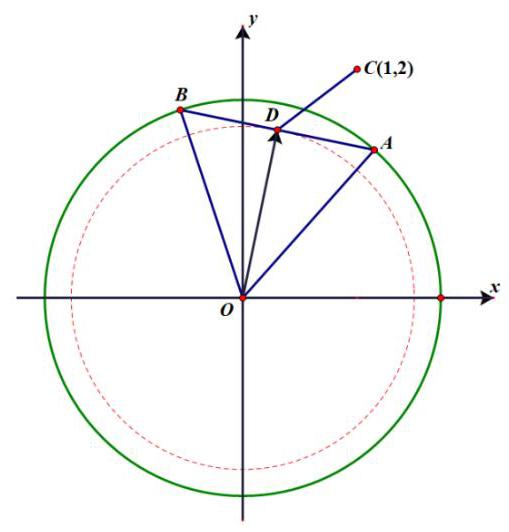
\includegraphics[max width=0.4\textwidth]{images/bo_d6dceus601uc73dvofhg_59_278_560_509_532_0.jpg}
\end{center}
\hspace*{3em} 

图 11-1

\begin{center}
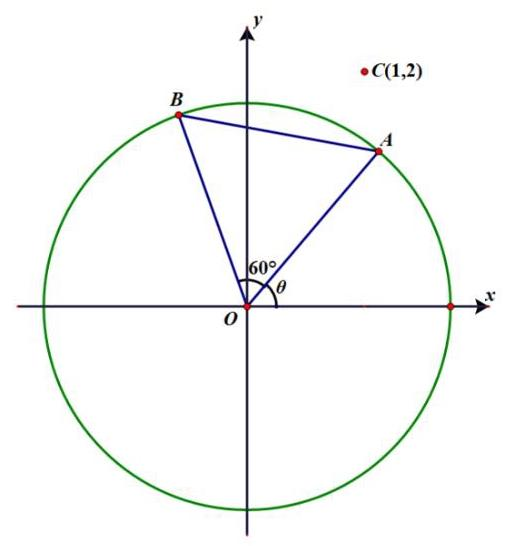
\includegraphics[max width=0.4\textwidth]{images/bo_d6dceus601uc73dvofhg_59_851_553_506_546_0.jpg}
\end{center}
\hspace*{3em} 

图 11-2

解法二 (坐标法): 依题意可得: \({\Delta OAB}\) 是一个边长为 \(\sqrt{3}\) 的等边三角形,如图 11-2 建系. 设 \(A\left( {\sqrt{3}\cos \theta ,\sqrt{3}\sin \theta }\right) ,B\left( {\sqrt{3}\cos \left( {\theta  + \frac{\pi }{3}}\right) ,\sqrt{3}\sin \left( {\theta  + \frac{\pi }{3}}\right) }\right)\) ,

则 \(\overrightarrow{AB} = \left( {-\frac{\sqrt{3}}{2}\cos \theta  - \frac{3}{2}\sin \theta , - \frac{\sqrt{3}}{2}\sin \theta  + \frac{3}{2}\cos \theta }\right) ,\overrightarrow{CA} = \left( {\sqrt{3}\cos \theta  - 1,\sqrt{3}\sin \theta  - 2}\right)\) ,

所以 \(2\overrightarrow{CA} + \overrightarrow{AB} = \left( {\frac{3\sqrt{3}}{2}\cos \theta  - \frac{3}{2}\sin \theta  - 2,\frac{3\sqrt{3}}{2}\sin \theta  + \frac{3}{2}\cos \theta  - 4}\right)\) ,

故 \(\left| {2\overrightarrow{CA} + \overrightarrow{AB}}\right|  = \sqrt{{\left( \frac{3\sqrt{3}}{2}\cos \theta  - \frac{3}{2}\sin \theta  - 2\right) }^{2} + {\left( \frac{3\sqrt{3}}{2}\sin \theta  + \frac{3}{2}\cos \theta  - 4\right) }^{2}}\)

\(= \sqrt{{29} - \left( {{12}\sqrt{3} - 6}\right) \sin \theta  - \left( {6\sqrt{3} + {12}}\right) \cos \theta } = \sqrt{{29} - {12}\sqrt{5}\sin \left( {\theta  - \varphi }\right) } \geq  \sqrt{{29} - {12}\sqrt{5}} = 2\sqrt{5} - 3\) .

\(\left| {2\overrightarrow{CA} + \overrightarrow{AB}}\right|\) 的最小值是 \(2\sqrt{5} - 3\) .

5.【2025.12 静安高三一模 11】如图,已知 \({AB}\) 是半圆 \(O\) 的直径,直径长为 2,点 \(C,D\) 均在半圆 \(\mathrm{O}\) 上,且都不与点 \(A,B\) 重合, \(A,B,C,D\) 四点依次按照逆时针方向排列. 若 \({CD}\) 的长为 \(\sqrt{2}\) ，则 \(\overrightarrow{AC} \cdot  \overrightarrow{BD}\) 的取值范围为\_\_\_\_\_.

\begin{center}
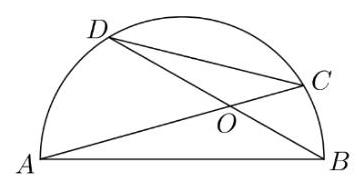
\includegraphics[max width=0.3\textwidth]{images/bo_d6dceus601uc73dvofhg_60_1046_217_357_186_0.jpg}
\end{center}
\hspace*{3em} 

【答案】 \(\lbrack  - \sqrt{2} - 1, - 2)\)

【解析】联结 \({OC},{OD}\) ,根据 \({CD} = 2\) 可得 \(\angle {COD} = \frac{\pi }{2}\) .

如图建系,可得 \(A\left( {-1,0}\right) ,B\left( {1,0}\right)\) ,设 \(C\left( {\cos \theta ,\sin \theta }\right)\) (其中 \(0 < \theta  < \frac{\pi }{2}\) ),

则 \(D\left( {\cos \left( {\theta  + \frac{\pi }{2}}\right) ,\sin \left( {\theta  + \frac{\pi }{2}}\right) }\right)\) ,化简得 \(D\left( {-\sin \theta ,\cos \theta }\right)\) .

从而可得 \(\overrightarrow{AC} = \left( {\cos \theta  + 1,\sin \theta }\right) ,\overrightarrow{BD} = \left( {-\sin \theta  - 1,\cos \theta }\right)\) ,

\(\therefore \overrightarrow{AC} \cdot  \overrightarrow{BD} = \left( {\cos \theta  + 1}\right) \left( {-\sin \theta  - 1}\right)  + \sin \theta \cos \theta  =  - \sin \theta  - \cos \theta  - 1 =  - \sqrt{2}\sin \left( {\theta  + \frac{\pi }{4}}\right)  - 1\) .

根据 \(0 < \theta  < \frac{\pi }{2}\) 可得 \(- \sqrt{2}\sin \left( {\theta  + \frac{\pi }{4}}\right)  - 1 \in  \left\lbrack  {-\sqrt{2} - 1, - 2}\right)\) ,

故 \(\overrightarrow{AC} \cdot  \overrightarrow{BD}\) 的取值范围为 \(\lbrack  - \sqrt{2} - 1, - 2)\) 。

\section*{6.3 向量综合}

1.【2025.12 宝山高三一模 9】已知等腰 \(\bigtriangleup {ABC}\) 中, \(A = \frac{\pi }{2},E,F\) 分别为 \({AB},{BC}\) 的中点, 若 \(\overrightarrow{BC} = \lambda \overrightarrow{AF} + \mu \overrightarrow{CE}\) ,则 \(\lambda  =\) \_\_\_\_\_.

【答案】 \(- \frac{2}{3}\)

【解析】设 \({AB} = {AC} = 2\) ,以点 \(A\) 为原点, \({AB},{AC}\) 分别为 \(x,y\) 轴建系,

则 \(A\left( {0,0}\right) ,B\left( {2,0}\right) ,C\left( {0,2}\right) ,E\left( {1,0}\right) ,F\left( {1,1}\right) ,\overrightarrow{BC} = \left( {-2,2}\right) ,\overrightarrow{AF} = \left( {1,1}\right) ,\overrightarrow{CE} = \left( {1, - 2}\right)\) .

代入 \(\overrightarrow{BC} = \lambda \overrightarrow{AF} + \mu \overrightarrow{CE}\) 得 \(\left( {-2,2}\right)  = \left( {\lambda  + \mu ,\lambda  - {2\mu }}\right)\) ， \(\therefore \left\{  \begin{array}{l} \lambda  + \mu  =  - 2 \\  \lambda  - {2\mu } = 2 \end{array}\right.\) ，解得 \(\left\{  \begin{array}{l} \lambda  =  - \frac{2}{3} \\  \mu  =  - \frac{4}{3} \end{array}\right.\) ，

2.【2025.12 普陀高三一模 11】设 \(P\) 是边长为 1 的正六边形 \({A}_{1}{A}_{2}{A}_{3}{A}_{4}{A}_{5}{A}_{6}\) 所在平面上的一点， 若点 \({A}_{1}\text{ 、 }{A}_{2}\text{ 、 }P\) 满足 \(\overrightarrow{P{A}_{1}} \cdot  \overrightarrow{P{A}_{2}} = 0\) ,则 \(\left| {\mathop{\sum }\limits_{{i = 1}}^{6}\overrightarrow{P{A}_{i}}}\right|\) 的最小值是\_\_\_\_\_.

【答案】 \(3\sqrt{3} - 3\)

【解析】依题意可得: 点 \(P\) 的轨迹是以 \({A}_{1}{A}_{2}\) 为直径的圆 \(\odot  M\) (点 \(M\) 为线段 \({A}_{1}{A}_{2}\) 的中点).

取六边形的几何中心 \(O\) ,则 \(\overrightarrow{P{A}_{i}} = \overrightarrow{PO} + \overrightarrow{O{A}_{i}}\left( {i = 1,2\cdots 6}\right)\) ,

\(\therefore \left| {\mathop{\sum }\limits_{{i = 1}}^{6}\overrightarrow{P{A}_{i}}}\right|  = \left| {6\overrightarrow{PO} + \mathop{\sum }\limits_{{i = 1}}^{6}\overrightarrow{O{A}_{i}}}\right|  = 6\left| \overrightarrow{PO}\right|\) .

而 \(\left| \overrightarrow{PM}\right|  + r \geq  \left| \overrightarrow{PO}\right|  \geq  \left| \overrightarrow{PM}\right|  - r\) ,即 \(\left| \overrightarrow{PO}\right|  \in  \left\lbrack  {\frac{\sqrt{3}}{2} - \frac{1}{2},\frac{\sqrt{3}}{2} + \frac{1}{2}}\right\rbrack\) ,当且仅当 \(O,P,M\) 三点共线时, 等号成立, \(\therefore \left| {\mathop{\sum }\limits_{{i = 1}}^{6}\overrightarrow{P{A}_{i}}}\right|  = 6\left| \overrightarrow{PO}\right|  \geq  3\sqrt{3} - 3\) ,即 \(\left| {\mathop{\sum }\limits_{{i = 1}}^{6}\overrightarrow{P{A}_{i}}}\right|\) 的最小值为 \(3\sqrt{3} - 3\) .

\begin{center}
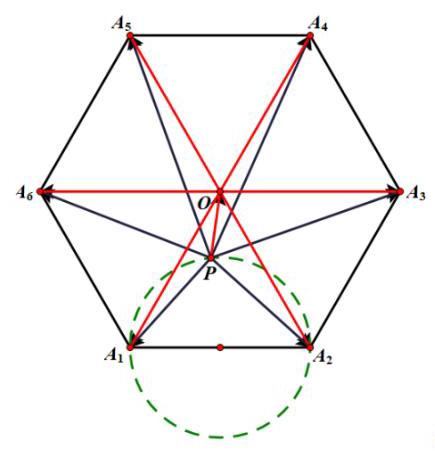
\includegraphics[max width=0.3\textwidth]{images/bo_d6dceus601uc73dvofhg_61_936_608_435_451_0.jpg}
\end{center}
\hspace*{3em} 

3.【2025.12 长宁高三一模 12】已知集合 \(\Omega  = \left\{  {\overrightarrow{w} \mid  \overrightarrow{w} = \lambda \overrightarrow{{e}_{1}} + \mu \overrightarrow{{e}_{2}} + \gamma \overrightarrow{{e}_{3}},\lambda ,\mu ,\gamma  \in  \{  - 1,1\} }\right\}\) ，若对于空间中任意单位向量 \(\overrightarrow{{e}_{1}},\overrightarrow{{e}_{2}},\overrightarrow{{e}_{3}}\) ，都存在 \(\overrightarrow{d} \in  \Omega\) ，使得 \(\left| \overrightarrow{d}\right|  \geq  r\) ，则实数 \(r\) 的最大值为\_\_\_\_\_.

【答案】 \(\sqrt{3}\)

【解析】当 \(\overrightarrow{d} \in  \left\{  {\overrightarrow{w}\left| {\;\overrightarrow{w} = \lambda \overrightarrow{{e}_{1}} + \mu \overrightarrow{{e}_{2}} + \gamma \overrightarrow{{e}_{3}}}\right. ,\lambda ,\mu ,\gamma  \in  \{  - 1,1\} }\right\}\) 时,则 \(\overrightarrow{d}\) 为一个“以 \(\overrightarrow{{e}_{1}},\overrightarrow{{e}_{2}},\overrightarrow{{e}_{3}}\) 为从同一顶点出发的三条棱构成的一个平行四面体”的体对角线. 考虑到 3 个单位向量 \(\overrightarrow{{e}_{1}},\overrightarrow{{e}_{2}},\overrightarrow{{e}_{3}}\) 的任意性, 不难得出: 当 \(\overrightarrow{{e}_{1}},\overrightarrow{{e}_{2}},\overrightarrow{{e}_{3}}\) 两两互相垂直时,此时构成一个棱长为 1 的正方体, \(\left| \overrightarrow{d}\right|\) 即为体对角线, 达到最大，此时 \({\left| \overrightarrow{d}\right| }_{\max } = \sqrt{3}\) ，故实数 \(r\) 的最大值为 \(\sqrt{3}\) . 3 定

4.【2025.12 黄浦高三一模 16】已知点 \(P\left( {-5,0}\right) ,{Q}_{1},{Q}_{2} \in  \left\{  {\left( {x,y}\right) \left| \right| x\left| { \leq  1,}\right| y \mid   \leq  1}\right\}\) ,则 \(\overrightarrow{P{Q}_{1}} \cdot  \overrightarrow{P{Q}_{2}}\) 的取值范围是( )

A. \(\left\lbrack  {{15},{36}}\right\rbrack\) B. \(\left\lbrack  {{15},{37}}\right\rbrack\) C. \(\left\lbrack  {{16},{36}}\right\rbrack\) D. \(\left\lbrack  {{16},{37}}\right\rbrack\)

【答案】B

【解析】当 \({Q}_{1}\left( {1,1}\right) ,{Q}_{2}\left( {1,1}\right)\) 时, \(\overrightarrow{P{Q}_{1}} = \left( {6,1}\right) ,\overrightarrow{P{Q}_{2}} = \left( {6,1}\right)\) ,此时 \({\left( \overrightarrow{P{Q}_{1}} \cdot  \overrightarrow{P{Q}_{2}}\right) }_{\max } = {37}\) ;

当 \({Q}_{1}\left( {-1,1}\right) ,{Q}_{2}\left( {-1, - 1}\right)\) 时, \(\overrightarrow{P{Q}_{1}} = \left( {4,1}\right) ,\overrightarrow{P{Q}_{2}} = \left( {4, - 1}\right)\) ,此时 \({\left( \overrightarrow{P{Q}_{1}} \cdot  \overrightarrow{P{Q}_{2}}\right) }_{\min } = {15}\) . \(\ll\)

\section*{第七章 解析几何}

\section*{7.1 直线与圆}

\section*{【直线知识梳理】}

1. 已知 \(A\left( {{x}_{1},{y}_{1}}\right) ,B\left( {{x}_{2},{y}_{2}}\right)\) ,则 \({k}_{AB} = \frac{{y}_{1} - {y}_{2}}{{x}_{1} - {x}_{2}}\left( {{x}_{1} \neq  {x}_{2}}\right)\)

\(\left| {AB}\right|  = \sqrt{{\left( {x}_{1} - {x}_{2}\right) }^{2} + {\left( {y}_{1} - {y}_{2}\right) }^{2}} = \sqrt{1 + {k}^{2}}\left| {{x}_{1} - {x}_{2}}\right|  = \sqrt{1 + \frac{1}{{k}^{2}}}\left| {{y}_{1} - {y}_{2}}\right|  = \sqrt{1 + {m}^{2}}\left| {{y}_{1} - {y}_{2}}\right|\)

2. 直线的方程: (应用以上直线方程时应考虑其存在的条件)

(1)点方向式: \(\frac{x - {x}_{0}}{u} = \frac{y - {y}_{0}}{v}\) (过 \(P\left( {{x}_{0},{y}_{0}}\right)\) ，一个方向向量为 \(\left( {u,v}\right)\) ， \({uv} \neq  0\) ) 当 \(u = 0\) 时,该直线方程为 \(x = {x}_{0}\) ; 当 \(v = 0\) 时,该直线方程为 \(y = {y}_{0}\)

(2)点法向式: \(a\left( {x - {x}_{0}}\right)  + b\left( {y - {y}_{0}}\right)  = 0\) (过 \(P\left( {{x}_{0},{y}_{0}}\right)\) ，一个法向量为 \(\left( {a,b}\right)\) )

(3)点斜式: \(y - {y}_{0} = k\left( {x - {x}_{0}}\right)\) (过 \(P\left( {{x}_{0},{y}_{0}}\right)\) ，斜率为 \(\mathrm{k}\) ) 当斜率不存在时,该直线方程为 \(x = {x}_{0}\)

(4)一般式: \({Ax} + {By} + C = 0\) (A、B 不同时为零)

(5)斜截式: \(y = {kx} + b\) (斜率为 \(\mathrm{k}\) ，在 \(\mathrm{y}\) 轴上的截距为 \(\mathrm{b}\) ) 当斜率不存在时,该直线方程为 \(x = 0\)

(6) 参数方程: \(\left\{  \begin{array}{l} x = {x}_{0} + {ut} \\  y = {y}_{0} + {vt} \end{array}\right.\) (过 \(P\left( {{x}_{0},{y}_{0}}\right)\) ,一个方向向量为 \(\left( {u,v}\right)\) )

(7)参数方程: \(\left\{  \begin{array}{l} x = {x}_{0} + t\cos \alpha \\  y = {y}_{0} + t\sin \alpha  \end{array}\right.\) (过 \(P\left( {{x}_{0},{y}_{0}}\right)\) ,倾斜角为 \(\alpha\) )

3. 直线斜率 \(k\) 和倾斜角 \(\alpha\) 的关系: 倾斜角 \(\alpha  \in  \lbrack 0,\pi )\)

若 \(k = \tan \alpha ,\alpha  \in  \left\lbrack  {0,\frac{\pi }{2}}\right)  \cup  \left( {\frac{\pi }{2},\pi }\right)\) ; \(\;\alpha  = \left\{  \begin{array}{l} \arctan k\;\left( {k > 0}\right) \\  \frac{\pi }{2}\;\left( {k\text{ 不存在 }}\right) \\  \pi  + \arctan k\left( {k < 0}\right)  \end{array}\right.\)

4、已知直线的法向量为 \(\overrightarrow{n} = \left( {a,b}\right)\) ,则该直线的方向向量为 \(\overrightarrow{d} = \left( {b, - a}\right)\) ,斜率为 \(k =  - \frac{a}{b}\) ( \(b \neq  0\) )

5. 两条直线的平行和垂直

(1)若 \({l}_{1} : y = {k}_{1}x + {b}_{1},\;{l}_{2} : y = {k}_{2}x + {b}_{2}\)

\({l}_{1}//{l}_{2} \Leftrightarrow  \left\{  \begin{array}{l} {k}_{1} = {k}_{2} \\  {b}_{1} \neq  {b}_{2} \end{array}\right.\) ; 此时两平行直线 \({l}_{1},{l}_{2}\) 间的距离 \(d = \frac{\left| {b}_{1} - {b}_{2}\right| }{\sqrt{1 + {k}^{2}}}\) ;

\({l}_{1} \bot  {l}_{2} \Leftrightarrow  {k}_{1}{k}_{2} =  - 1\) ,或一个为零,另一个不存在。

(2)若 \({l}_{1} : {A}_{1}x + {B}_{1}y + {C}_{1} = 0,{l}_{2} : {A}_{2}x + {B}_{2}y + {C}_{2} = 0\)

\({l}_{1}//{l}_{2} \Leftrightarrow\) 此时两平行直线 \({l}_{1},{l}_{2}\) 间的距离 \(d = \frac{\left| {C}_{1} - {C}_{2}\right| }{\sqrt{{A}^{2} + {B}^{2}}}\) ;

\({l}_{1} \bot  {l}_{2} \Leftrightarrow  {A}_{1}{A}_{2} + {B}_{1}{B}_{2} = 0\) 。

6.两直线夹角公式:

(1) \(\tan \theta  = \left| \frac{{k}_{2} - {k}_{1}}{1 + {k}_{1}{k}_{2}}\right| \left( {{l}_{1} : y = {k}_{1}x + {b}_{1},{l}_{2} : y = {k}_{2}x + {b}_{2}}\right)\)

(2) \(\cos \theta  = \frac{\left| {A}_{1}{A}_{2} + {B}_{1}{B}_{2}\right| }{\sqrt{{A}_{1}^{2} + {B}_{1}^{2}}\sqrt{{A}_{2}^{2} + {B}_{2}^{2}}}\left( {{l}_{1} : {A}_{1}x + {B}_{1}y + {C}_{1} = 0,{l}_{2} : {A}_{2}x + {B}_{2}y + {C}_{2} = 0}\right)\)

7. 常见的直线系方程:

(1)定点直线系方程:经过定点 \(P\left( {{x}_{0},{y}_{0}}\right)\) 的直线系方程为 \(y - {y}_{0} = k\left( {x - {x}_{0}}\right)\) (除直线 \(\left. {x = {x}_{0}}\right)\) ,其中 \(\mathrm{k}\) 是待定的系数。

(2)共点直线系方程:经过两直线 \({l}_{1} : {A}_{1}x + {B}_{1}y + {C}_{1} = 0,{l}_{2} : {A}_{2}x + {B}_{2}y + {C}_{2} = 0\) 的交点的直线系方程为 \({A}_{1}x + {B}_{1}y + {C}_{1} + \lambda \left( {{A}_{2}x + {B}_{2}y + {C}_{2}}\right)  = 0\) (除 \(\left. {1}_{2}\right)\) ,其中 \(\lambda\) 是待定的系数。

(3)平行直线系方程:与直线 \({Ax} + {By} + C = 0\) 平行的直线系方程为 \({Ax} + {By} + {C}^{\prime } = 0\left( {{C}^{\prime } \neq  C}\right)\) 。

(4)垂直直线系方程:与直线 \({Ax} + {By} + C = 0\) 垂直的直线系方程为 \({Bx} - {Ay} + {C}^{\prime } = 0\) 。

8. 点 \(P\left( {{x}_{0},{y}_{0}}\right)\) 到直线 \({Ax} + {By} + C = 0\) 的距离 \(\mathrm{d} = \frac{\left| A{x}_{0} + B{y}_{0} + C\right| }{\sqrt{{A}^{2} + {B}^{2}}}\) 。

9. \(\delta  = \frac{a{x}_{0} + b{y}_{0} + c}{\sqrt{{a}^{2} + {b}^{2}}}\) 的符号确定了点 \(P\left( {{x}_{0},{y}_{0}}\right)\) 关于直线 \(l : {ax} + {by} + c = 0\) 的相对位置。在直线同侧的所有点， \(\delta\) 的符号是相同的，在直线异侧的所有点， \(\delta\) 的符号是相反的。(填写“相同”或“相反”)

10. 点 \(A\left( {{x}_{1},{y}_{1}}\right) ,B\left( {{x}_{2},{y}_{2}}\right)\) 在直线 \({Ax} + {By} + C = 0\) 异侧 (同侧)

\[
\Leftrightarrow  \left( {A{x}_{1} + B{y}_{1} + C}\right) \left( {A{x}_{2} + B{y}_{2} + C}\right)  < 0\;\left( { > 0}\right) \text{ 。 }
\]

\section*{【圆知识梳理】}

\section*{1. 圆的定义及其方程}

(1)圆是到一个定点的距离等于定长 (大于零) 的点的轨迹. 这个定点就是圆心, 定长就是圆的半径.

(2)圆的标准方程: \({\left( x - a\right) }^{2} + {\left( y - b\right) }^{2} = {r}^{2}\left( {r > 0}\right)\) 是以点 \(\left( {a,b}\right)\) 为圆心， \(r\) 为半径的圆的方程， 叫做圆的标准方程.

(3)圆的一般方程:当 \({D}^{2} + {E}^{2} - {4F} > 0\) 时，二元二次方程 \({x}^{2} + {y}^{2} + {Dx} + {Ey} + F = 0\) 叫做圆的一般方程. 圆心为 \(\left( {-\frac{D}{2}, - \frac{E}{2}}\right)\) ,半径长为 \(\frac{\sqrt{{D}^{2} + {E}^{2} - {4F}}}{2}\) .

\section*{2. 点与圆的位置关系}

设点 \({P}_{0}\left( {{x}_{0},{y}_{0}}\right)\) ,圆的标准方程为 \({\left( x - a\right) }^{2} + {\left( y - b\right) }^{2} = {r}^{2}\) ,则

 \circled{1}  \({\left( {x}_{0} - a\right) }^{2} + {\left( {y}_{0} - b\right) }^{2} = {r}^{2} \Leftrightarrow\) 点在圆上；

 \circled{2}  \({\left( {x}_{0} - a\right) }^{2} + {\left( {y}_{0} - b\right) }^{2} > {r}^{2} \Leftrightarrow\) 点在圆外;

 \circled{3}  \({\left( {x}_{0} - a\right) }^{2} + {\left( {y}_{0} - b\right) }^{2} < {r}^{2} \Leftrightarrow\) 点在圆内.

\section*{3. 直线与圆的位置关系(半径为 \(r\) ，圆心到直线的距离为 \(d\) )}

\begin{center}
\adjustbox{max width=\textwidth}{
\begin{tabular}{|c|c|c|c|c|}
\hline
\phantom{X} & \phantom{X} & 相离 & 相切 & 相交 \\
\cline{1-5}
\multicolumn{2}{|c|}{图形} & 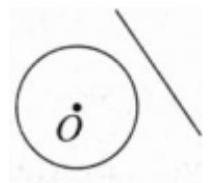
\includegraphics[max width=0.2\textwidth]{images/bo_d6dceus601uc73dvofhg_65_711_1383_212_183_0.jpg} & 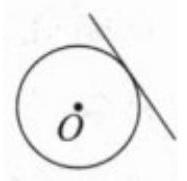
\includegraphics[max width=0.2\textwidth]{images/bo_d6dceus601uc73dvofhg_65_962_1392_187_181_0.jpg} & 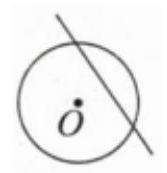
\includegraphics[max width=0.2\textwidth]{images/bo_d6dceus601uc73dvofhg_65_1199_1392_167_173_0.jpg} \\
\cline{1-5}
\multirow{2}{*}{量化} & 方程观点 & \(\Delta  < 0\) & \(\Delta  = 0\) & \(\Delta  > 0\) \\
\cline{2-5}
 & 几何观点 & \(d > r\) & \(d = r\) & \(d < r\) \\
\cline{1-5}
\hline
\end{tabular}
}
\end{center}

(1)圆的切线方程常用结论

 \circled{1} 过圆 \({x}^{2} + {y}^{2} = {r}^{2}\) 上一点 \(P\left( {{x}_{0},{y}_{0}}\right)\) 的圆的切线方程为 \({x}_{0}x + {y}_{0}y = {r}^{2}\) .

 \circled{2}  过 圆 \({\left( x - a\right) }^{2} + {\left( y - b\right) }^{2} = {r}^{2}\) 上一点 \(P\left( {{x}_{0},{y}_{0}}\right)\) 的 圆的 切 线 方 程 为 \(\left( {{x}_{0} - a}\right) \left( {x - a}\right)  + \left( {{y}_{0} - b}\right) \left( {y - b}\right)  = r.\)

 \circled{3}  过圆 \({x}^{2} + {y}^{2} = {r}^{2}\) 外一点 \(M\left( {{x}_{0},{y}_{0}}\right)\) 作圆的两条切线,则两切点所在直线方程为 \({x}_{0}x + {y}_{0}y = {r}^{2}.\)

(2)有关弦长问题的两种求法

\begin{center}
\adjustbox{max width=\textwidth}{
\begin{tabular}{|c|c|}
\hline
几何法 & 直线被圆截得的半弦长 \(\frac{1}{2}\left| {AB}\right|\) ,弦心距 \(d\) 和圆的半径 \(r\) 构成直角三角形,即 \(\left| {AB}\right|  = 2\sqrt{{r}^{2} - {d}^{2}}\) \\
\cline{1-2}
代数法 & 联立直线方程和圆的方程,消元转化为关于 \(x\) 的一元二次方程,由根与系数的关系即可求得弦长 \(\left| {AB}\right|  = \sqrt{1 + {k}^{2}}\left| {{x}_{1} - {x}_{2}}\right|  = \sqrt{1 + {k}^{2}}\sqrt{{\left( {x}_{1} + {x}_{2}\right) }^{2} - 4{x}_{1}{x}_{2}}\) 或 \(\left| {AB}\right|  = \sqrt{1 + \frac{1}{{k}^{2}}}\left| {{y}_{1} - {y}_{2}}\right|  = \sqrt{1 + \frac{1}{{k}^{2}}}\sqrt{{\left( {y}_{1} + {y}_{2}\right) }^{2} - 4{y}_{1}{y}_{2}}\) \\
\cline{1-2}
\hline
\end{tabular}
}
\end{center}

4. 圆与圆的位置关系(两圆半径为 \({r}_{1},{r}_{2},d = \left| {{O}_{1}{O}_{2}}\right|\) )

\begin{center}
\adjustbox{max width=\textwidth}{
\begin{tabular}{|c|c|c|}
\hline
\phantom{X} & 图形 & 量的关 \\
\cline{1-3}
相离 & 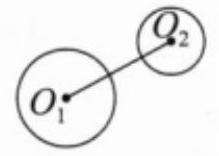
\includegraphics[max width=0.2\textwidth]{images/bo_d6dceus601uc73dvofhg_66_579_1013_219_156_0.jpg} & \(d > {r}_{1} + {r}_{2}\) \\
\cline{1-3}
外切 & 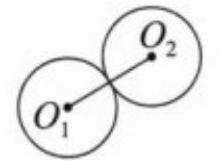
\includegraphics[max width=0.2\textwidth]{images/bo_d6dceus601uc73dvofhg_66_575_1189_220_161_0.jpg} & \(d = {r}_{1} + {r}_{2}\) \\
\cline{1-3}
相交 & 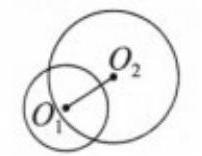
\includegraphics[max width=0.2\textwidth]{images/bo_d6dceus601uc73dvofhg_66_587_1368_202_156_0.jpg} & \(\left| {{r}_{1} - {r}_{2}}\right|  < d < {r}_{1} + {r}_{2}\) \\
\cline{1-3}
内切 & 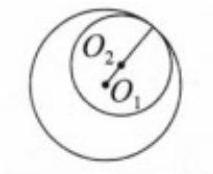
\includegraphics[max width=0.2\textwidth]{images/bo_d6dceus601uc73dvofhg_66_575_1551_213_174_0.jpg} & \(d = \left| {{r}_{1} - {r}_{2}}\right|\) \\
\cline{1-3}
内含 & 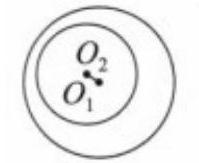
\includegraphics[max width=0.2\textwidth]{images/bo_d6dceus601uc73dvofhg_66_580_1753_199_163_0.jpg} & \(d < \left| {{r}_{1} - {r}_{2}}\right|\) \\
\cline{1-3}
\hline
\end{tabular}
}
\end{center}

1.【2025.12 黄浦高三一模 2】若直线 \({l}_{1} : x + {2y} - 1 = 0\) 与 \({l}_{2} : {ax} - {4y} + 5 = 0\) 平行，则 \(a =\) \_\_\_\_\_.

【答案】 \(a =  - 2\)

【解析】两直线的法向量分别为 \(\overrightarrow{{n}_{1}} = \left( {1,2}\right) ,\overrightarrow{{n}_{2}} = \left( {a, - 4}\right)\) ,由 \(\overrightarrow{{n}_{1}}//\overrightarrow{{n}_{2}}\) 得 \(a =  - 2\) 。

2.【2025.12 嘉定高三一模 2】已知直线 \(l\) 经过点 \(\left( {-1, - 1}\right)\) 、 \(\left( {2,2}\right)\) ，则 \(l\) 的倾斜角为\_\_\_\_\_. 【答案】 \(\frac{\pi }{4}\)

【解析】易得斜率 \(k = 1\) ,所以倾斜角为 \(\frac{\pi }{4}\) .

3.【2025.12 静安高三一模 3】已知直线 \({l}_{1} : {3x} - \sqrt{3}y + {10} = 0\) 与 \({l}_{2} : x - \sqrt{3}y = 0\) ，则直线 \({l}_{1}\) 与 \({l}_{2}\) 的夹角大小是\_\_\_\_\_.

【答案】 \(\frac{\pi }{6}\)

【解析】依题意可得: \({l}_{1}\) 与 \({l}_{2}\) 的斜率分别为 \({k}_{1} = \sqrt{3},{k}_{2} = \frac{\sqrt{3}}{3}\) ,倾斜角分别为 \({\alpha }_{1} = \frac{\pi }{3},{\alpha }_{2} = \frac{\pi }{6}\) ,所以夹角为 \(\theta  = \frac{\pi }{6}\) . 令

4.【2025.12 奉贤高三一模 4】已知向量 \(\overrightarrow{a} = \left( {1,1}\right)\) ，则经过点 \(\left( {1,0}\right)\) 且与 \(\overrightarrow{a}\) 垂直的直线方程为\_\_\_\_\_.

【答案】 \(x + y - 1 = 0\)

【解析】过 \(\left( {1,0}\right)\) 且法向量为 \(\overrightarrow{a} = \left( {1,1}\right)\) 的直线方程为: \(\left( {x - 1}\right)  + y = 0\) ,即 \(x + y - 1 = 0\) .

5.【2025.12 闵行高三一模 6】过点 \(P\left( {1,1}\right)\) 的直线被圆 \({x}^{2} + {y}^{2} = 4\) 截得的最短弦长为\_\_\_\_\_.

【答案】 \(2\sqrt{2}\)

【解析】截得的最短弦长为 \(2\sqrt{4 - \left\lbrack  {{\left( 1 - 0\right) }^{2} + {\left( 1 - 0\right) }^{2}}\right\rbrack  } = 2\sqrt{2} \ll\)

6.【2025.12 杨浦高三一模 7】圆 \(C : {\left( x - 5\right) }^{2} + {\left( y - 3\right) }^{2} = {10}\) 的圆心到直线 \(l : x - y + 2 = 0\) 的距离为\_\_\_\_\_.

【解析】依题意可得: 圆心为 \(\left( {5,3}\right) ,\therefore d = \frac{\left| 5 - 3 + 2\right| }{\sqrt{2}} = 2\sqrt{2} \cdot  3 <\)

7.【2025.12 普陀高三一模 9】设 \(m \in  \mathbf{R}\) ，直线 \(l : {2x} + y + m = 0\) 经过点 \(P\) ，若向量 \(\overline{PQ} = \left( {1,3}\right)\) ， 则点 \(Q\) 到直线 \(l\) 的距离为\_\_\_\_\_.

【答案】 \(\sqrt{5}\)

【解析】依题意可得: 直线 \(l\) 和直线 \({PQ}\) 的一个法向量分别为 \(\overrightarrow{{n}_{l}} = \left( {2,1}\right) ,\overrightarrow{{n}_{PQ}} = \left( {3, - 1}\right)\) ,所以直线 \(l\) 和直线 \({PQ}\) 的夹角为 \(\cos \theta  = \cos \left\langle  {\overrightarrow{{n}_{l}},\overrightarrow{{n}_{PQ}}}\right\rangle   = \frac{\left| \overrightarrow{{n}_{l}} \cdot  \overrightarrow{{n}_{PQ}}\right| }{\left| \overrightarrow{{n}_{l}}\right| \left| \overrightarrow{{n}_{PQ}}\right| } = \frac{\sqrt{2}}{2}\) ,

\(\therefore\) 点 \(Q\) 到直线 \(l\) 的距离为 \(d = \cos \theta  \cdot  \left| \overrightarrow{PQ}\right|  = \sqrt{5}\) .

8.【 2025.12 青浦高三一模 10】设 \(A\) 为圆 \({x}^{2} + {\left( y + 1\right) }^{2} = 1\) 上的动点, \({PA}\) 是圆的切线,且 \(\left| {PA}\right|  = 1\) , 则点 \(P\) 的轨迹方程是\_\_\_\_\_.

【答案】 \({x}^{2} + {\left( y + 1\right) }^{2} = 2\)

【答案】圆心为 \(M\left( {0, - 1}\right)\) ,半径为 1,联结 \({MP}\) .

则由 \(\left| {PA}\right|  = 1\) 可得 \({MP} = \sqrt{A{M}^{2} + A{P}^{2}} = \sqrt{2}\) ， \(\therefore\) 点 \(P\) 的轨迹方程 \({x}^{2} + {\left( y + 1\right) }^{2} = 2\) .

9.【2025.12 奉贤高三一模 10】已知两个非负实数 \(a\text{ 、 }b\) 满足 \(a + {2b} = 2\) ,则 \({\left( a - 1\right) }^{2} + {\left( b - 4\right) }^{2}\) 的最小值是\_\_\_\_\_.

【答案】 10

【解析】依题意可得: \(\left\{  \begin{array}{l} b \geq  0 \\  a = 2 - {2b} \geq  0 \end{array}\right.\) ,解得 \(1 \geq  b \geq  0\) ,

\(\therefore {\left( a - 1\right) }^{2} + {\left( b - 4\right) }^{2} = {\left( 1 - 2b\right) }^{2} + {\left( b - 4\right) }^{2} = 5{b}^{2} - {12b} + {17} = 5{\left( b - \frac{6}{5}\right) }^{2} + \frac{49}{5}\) .

当 \(1 \geq  b \geq  0\) 时,函数 \(f\left( b\right)  = 5{\left( b - \frac{6}{5}\right) }^{2} + \frac{49}{5}\) 单调递减, \(\therefore f{\left( b\right) }_{\min } = f\left( 1\right)  = {10}\) .

【注意】本题的一种易错解法是:

\({\left( a - 1\right) }^{2} + {\left( b - 4\right) }^{2}\) 表示直线 \(x + {2y} - 2 = 0\) 上的动点 \(\left( {a,b}\right)\) 到定点 \(\left( {1,4}\right)\) 的距离的平方,求其最小值可进而转化为点 \(\left( {1,4}\right)\) 到直线 \(x + {2y} - 2 = 0\) 的距离并平方.

\section*{7.2 椭圆}

\section*{【知识梳理】}

\section*{1. 椭圆的定义}

平面上到两个定点 \({F}_{1},{F}_{2}\) 的距离之和等于常数 \({2a}\left( {{2a} > \left| {{F}_{1}{F}_{2}}\right| }\right)\) 的点的轨迹叫做椭圆.

当 \({2a} > {2c}\) 时,轨迹是椭圆;

当 \({2a} = {2c}\) 时,轨迹是一条线段 \({F}_{1}{F}_{2}\) ;

当 \({2a} < {2c}\) 时,轨迹不存在.

这两个定点 \({F}_{1},{F}_{2}\) 叫做椭圆的焦点,两个焦点间的距离 \(\left| {{F}_{1}{F}_{2}}\right|\) 叫做焦距.

\section*{2. 椭圆的标准方程}

焦点在 \(x\) 轴上时: \(\frac{{x}^{2}}{{a}^{2}} + \frac{{y}^{2}}{{b}^{2}} = 1\left( {a > b > 0}\right)\) ;

焦点在 \(y\) 轴上时, \(\frac{{y}^{2}}{{a}^{2}} + \frac{{x}^{2}}{{b}^{2}} = 1\left( {a > b > 0}\right)\) ;

其中 \({c}^{2} = {a}^{2} - {b}^{2}\) .

求椭圆的标准方程,必须先确定焦点所在的位置,再求出 \(a\text{ 、 }b\) 的值,需要两个独立的条件, 通常用待定系数法.

\section*{3. 椭圆的几何性质}

\begin{center}
\adjustbox{max width=\textwidth}{
\begin{tabular}{|c|c|c|c|}
\hline
条件 & \multicolumn{3}{|c|}{\({2a} > {2c},{a}^{2} = {b}^{2},a > 0,b > 0,c > 0\)} \\
\cline{1-4}
图像 & 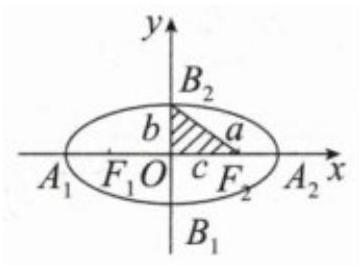
\includegraphics[max width=0.3\textwidth]{images/bo_d6dceus601uc73dvofhg_69_502_1405_359_265_0.jpg} & \multicolumn{2}{|c|}{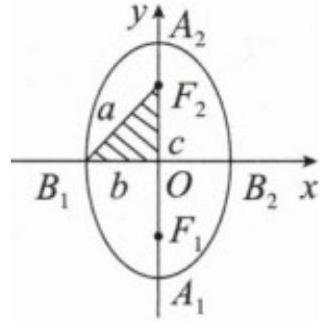
\includegraphics[max width=0.2\textwidth]{images/bo_d6dceus601uc73dvofhg_69_999_1383_333_322_0.jpg}} \\
\cline{1-4}
标准方程 & 焦 点 在 \(x\) 轴上时: \(\frac{{x}^{2}}{{a}^{2}} + \frac{{y}^{2}}{{b}^{2}} = 1\left( {a > b > 0}\right)\) & \multicolumn{2}{|c|}{焦 点 在 \(y\) 轴上时, \(\frac{{y}^{2}}{{a}^{2}} + \frac{{x}^{2}}{{b}^{2}} = 1\left( {a > b > 0}\right)\)} \\
\cline{1-4}
\multirow{10}{*}{\makecell{ 几何性 \\ 焦点 \\ 坐标 \\ 顶点质 }} & \({F}_{1}\left( {-c,0}\right) ,\;{F}_{2}\left( {c,0}\right)\) & \multicolumn{2}{|c|}{\({F}_{1}\left( {0, - c}\right) ,\;{F}_{2}\left( {0,c}\right)\)} \\
\cline{2-4}
 & \({A}_{1}\left( {-a,0}\right) ,\;{A}_{2}\left( {a,0}\right) ;\;{B}_{1}\left( {0, - b}\right) ,\) & \multicolumn{2}{|c|}{\({A}_{1}\left( {0, - a}\right) ,\;{A}_{2}\left( {0,a}\right) ;\;{B}_{1}\left( {-b,0}\right) ,\)} \\
\cline{2-4}
 &  &  &  \\
\cline{2-4}
 & 范围 & \(\left| x\right|  \leq  a,\;\left| y\right|  \leq  b\) & \(\left| x\right|  \leq  b,\;\left| y\right|  \leq  a\) \\
\cline{2-4}
 & \makecell{ 对称 \\ 性 } & \multicolumn{2}{|c|}{对称性关于 \(x,y\) 轴均对称,关于原点中心对称} \\
\cline{2-4}
 & 轴 & \multicolumn{2}{|c|}{轴长轴 \({A}_{1}{A}_{2}\) 的长为 \({2a}\) ,短轴 \({B}_{1}{B}_{2}\) 的长为 \({2b}\)} \\
\cline{2-4}
 & 焦距 & \multicolumn{2}{|c|}{\(\left| {{F}_{1}{F}_{2}}\right|  = {2c}\)} \\
\cline{2-4}
 & \makecell{ 离心 \\ 率 } & \multicolumn{2}{|c|}{\(e = \frac{c}{a},\;e \in  \left( {0,1}\right)\)} \\
\cline{2-4}
 & \(a,b\) , \(c\) 的关系 & \multicolumn{2}{|c|}{\(c = \sqrt{{a}^{2} - {b}^{2}}\)} \\
\cline{2-4}
 & 焦点三角形面积 & \multicolumn{2}{|c|}{\({S}_{\bigtriangleup P{F}_{1}{F}_{2}} = {b}^{2}\tan \frac{\angle {F}_{1}P{F}_{2}}{2}\)} \\
\cline{1-4}
\hline
\end{tabular}
}
\end{center}

1.【2025.12 静安高三一模 2】已知椭圆的标准方程为 \(\frac{{x}^{2}}{9} + \frac{{y}^{2}}{25} = 1\) ,则该椭圆的长轴的长等于\_\_\_\_\_.

【答案】 10

【解析】依题意可得: \(a = 5,b = 3\) ,所以长轴为 \({2a} = {10}\) . \(\approx\)

2.【 2025.12 奉贤高三一模 11】在平面中, \(\overrightarrow{{e}_{1}}\) 和 \(\overrightarrow{{e}_{2}}\) 是互相垂直的单位向量,向量 \(\overrightarrow{a}\) 满足 \(\left| {\overrightarrow{a} - 6\overrightarrow{{e}_{1}}}\right|  = 1\) ，向量 \(\overrightarrow{b}\) 满足 \(\left| {\overrightarrow{b} - 6\overrightarrow{{e}_{1}}}\right|  + \left| {\overrightarrow{b} - 8\overrightarrow{{e}_{2}}}\right|  = {20}\) ，则 \(\left| {\overrightarrow{a} - \overrightarrow{b}}\right|\) 的最大值是\_\_\_\_\_.

【答案】 16

【解析】建系,设 \({\overrightarrow{e}}_{1} = \left( {1,0}\right) ,{\overrightarrow{e}}_{2} = \left( {0,1}\right)\) ,再设 \(\overrightarrow{a} = \overrightarrow{OA},\overrightarrow{b} = \overrightarrow{OB},6{\overrightarrow{e}}_{1} = \overrightarrow{O{F}_{2}},8{\overrightarrow{e}}_{2} = \overrightarrow{O{F}_{1}}\) .

由 \(\left| {\overrightarrow{a} - 6\overrightarrow{{e}_{1}}}\right|  = 1\) 可得点 \(A\) 的轨迹为一个以 \({F}_{2}\left( {6,0}\right)\) 为圆心,半径为 1 的圆;

由 \(\left| {\overrightarrow{b} - 6\overrightarrow{{e}_{1}}}\right|  + \left| {\overrightarrow{b} - 8\overrightarrow{{e}_{2}}}\right|  = {20}\) 可得点 \(B\) 的轨迹为一个以 \({F}_{1}\left( {0,8}\right) ,{F}_{2}\left( {6,0}\right)\) 为焦点的椭圆,长轴长 \({2a} = {20}\) ,焦距为 \({2c} = {10}\) ; 如下图所示:

\begin{center}
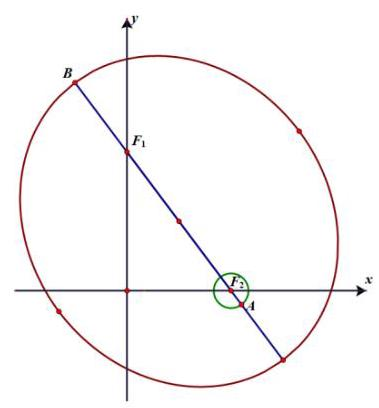
\includegraphics[max width=0.3\textwidth]{images/bo_d6dceus601uc73dvofhg_71_1026_993_379_408_0.jpg}
\end{center}
\hspace*{3em} 

而 \(\left| {\overrightarrow{a} - \overrightarrow{b}}\right|  = \left| \overrightarrow{AB}\right|\) 表示圆上一动点 \(A\) 与椭圆上一动点 \(B\) 之间距离的最大值.

\(\therefore \left| \overrightarrow{AB}\right|  \leq  \left| \overrightarrow{A{F}_{2}}\right|  + r \leq  a + c + r = {10} + 5 + 1 = {16}\) ,当且仅当点 \(B\) 在左上顶点,点 \(A\) 在圆与椭圆实轴的右下交点处，等号成立。

3.【2025.12 徐汇高三一模 15】设 \(P\) 为椭圆 \(\frac{{x}^{2}}{25} + \frac{{y}^{2}}{16} = 1\) 上一动点， \(M\) ， \(N\) 分别为圆 \({C}_{1} : {\left( x + 3\right) }^{2} + {y}^{2} = 1\) 和圆 \({C}_{2} : {\left( x - 3\right) }^{2} + {y}^{2} = 4\) 上的动点，则 \(\left| {PM}\right|  + \left| {PN}\right|\) 不可能为( ).

A. 7.5 B. 9.5 C. 11.5 D. 13.5

【答案】D

【解析】依题意可得: \(\left( {\left| {P{C}_{1}}\right|  - r}\right)  + \left( {\left| {P{C}_{2}}\right|  - R}\right)  \leq  \left| {PM}\right|  + \left| {PN}\right|  \leq  \left( {\left| {P{C}_{1}}\right|  + r}\right)  + \left( {\left| {P{C}_{2}}\right|  + R}\right)\) ,而根据椭圆定义有 \(\left| {P{C}_{1}}\right|  + \left| {P{C}_{2}}\right|  = {10}\) ， \(\therefore 7 \leq  \left| {PM}\right|  + \left| {PN}\right|  \leq  {13}\) ，故不可能 13.5，选 D.K

4.【2025.12 浦东高三一模 15】如图,椭圆 \({C}_{1}\text{ 、 }{C}_{2}\) 的离心率分别为 \({e}_{1}\text{ 、 }{e}_{2}\) ,双曲线 \({C}_{3}\text{ 、 }{C}_{4}\) 的离心率分别为 \({e}_{3}\text{ 、 }{e}_{4}\) ,则下列结论正确的是 ( )

A. \({e}_{3} > {e}_{4} > {e}_{2} > {e}_{1}\) B. \({e}_{4} > {e}_{3} > {e}_{1} > {e}_{2}\)

C. \({e}_{3} > {e}_{4} > {e}_{1} > {e}_{2}\) D. \({e}_{4} > {e}_{3} > {e}_{2} > {e}_{1}\)

\begin{center}
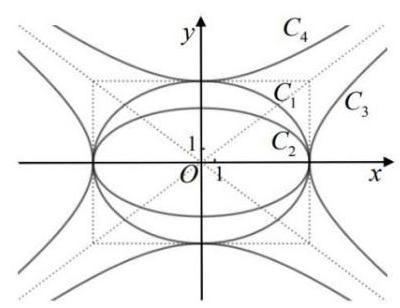
\includegraphics[max width=0.3\textwidth]{images/bo_d6dceus601uc73dvofhg_72_990_543_400_308_0.jpg}
\end{center}
\hspace*{3em} 

(第 15 题图)

【答案】D

【解析】在椭圆中, \({e}^{2} = \frac{{c}^{2}}{{a}^{2}} = \frac{{a}^{2} - {b}^{2}}{{a}^{2}} = 1 - \frac{{b}^{2}}{{a}^{2}}\) , \(\therefore\) 由 \({b}_{1} > {b}_{2}\) 得 \({e}_{1} < {e}_{2} < 1\) ;

在双曲线中, \({e}_{3}{}^{2} = \frac{{c}^{2}}{{a}^{2}} = \frac{{a}^{2} + {b}^{2}}{{a}^{2}} = 1 + \frac{{b}^{2}}{{a}^{2}},{e}_{4}{}^{2} = \frac{{c}^{2}}{{b}^{2}} = \frac{{a}^{2} + {b}^{2}}{{b}^{2}} = 1 + \frac{{a}^{2}}{{b}^{2}}\) ,

由于 \(a > b\) ， \(\therefore 1 < {e}_{3} < {e}_{4}\) . 综上所述: \({e}_{1} < {e}_{2} < 1 < {e}_{3} < {e}_{4}\) ，故选 D. \(\gg\)

5.【2025.12 崇明高三一模 16】已知点 \(A\left( {-2,0}\right) ,B\left( {2,0}\right)\) . 点 \(P\left( {m,n}\right)\) 在曲线 \(y = \sqrt{1 - \frac{{x}^{2}}{4}}\) 上. 记 \(\angle {APB} = \alpha\) ,则存在函数 \(y = f\left( x\right)\) ,对曲线上的任意一点 \(P\) 都有( )

A. \(m = f\left( \alpha \right)\) B. \(\alpha  = f\left( m\right)\) C. \(n = f\left( \alpha \right)\) D. \(\alpha  = f\left( n\right)\)

【答案】B

【解析】易知曲线 \(y = \sqrt{1 - \frac{{x}^{2}}{4}}\) 为上半椭圆,图像关于 \(y\) 轴对称,

当点 \(P\) 分别位于图像上关于 \(y\) 轴对称的 2 个点 \({P}_{1},{P}_{2}\) 时,显然 \(\angle A{P}_{2}B \neq  \angle A{P}_{1}B\) ,

即一个 \(n\) 对应有 2 个点 \(\alpha\) ,排除 \(\mathrm{D}\) ;

设线段 \({AB}\) 与半椭圆交于点 \(M\) . 当点 \(P\) 位于点 \(M\) 左侧某一位置 \({P}_{1}\) 时,此时 \(\angle A{P}_{1}B = \alpha\) ,则在点 \(M\) 的右侧,也必然存在某一点 \({P}_{3}\) (此时 \({P}_{3}\) 并不是与 \({P}_{1}\) 关于点 \(M\) 对称),

使得 \(\angle A{P}_{3}B = \angle A{P}_{1}B = \alpha\) ,即此时一个 \(\alpha\) 对应有 2 个点 \(P\) ,也即一个 \(\alpha\) 对应有 2 个 \(m\) ,也对

应有2个 \(n\) ,排除 \(\mathrm{A}/\mathrm{C}\) ;

对 \(\mathrm{B}\) 选项,也可以这么正面理解: 当 \(m \in  \left( {-2,2}\right)\) 时, \(m\) 每去一个值,点 \(P\) 都有一个确切的位置与之对应,此时 \(\angle {APB}\) 也就是一个确切的值,故一个 \(m\) 只对应一个 \(\alpha\) ,满足函数的定义.

\begin{center}
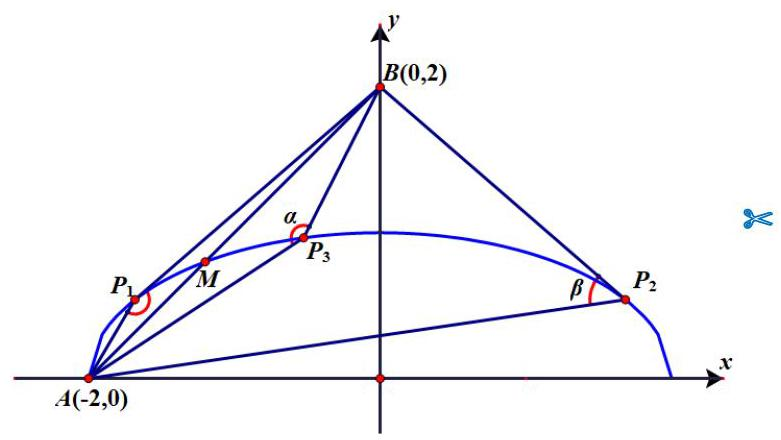
\includegraphics[max width=0.6\textwidth]{images/bo_d6dceus601uc73dvofhg_73_630_438_781_440_0.jpg}
\end{center}
\hspace*{3em} 

6.【2025.12 杨浦高三一模 20】已知椭圆 \(C : \frac{{x}^{2}}{{a}^{2}} + \frac{{y}^{2}}{2} = 1\left( {a > \sqrt{2}}\right)\) ,过动点 \(M\left( {0,m}\right)\) 的直线交 \(x\) 轴于点 \(N\) ,交椭圆 \(C\) 于 \(A,P\) (点 \(P\) 在第一象限),过点 \(P\) 作 \(x\) 轴的垂线交椭圆 \(C\) 于另一点 \(Q\) ,延长 \({QM}\) 交椭圆 \(C\) 于点 \(B\) .

(1)若椭圆 \(C\) 的离心率为 \(\frac{\sqrt{3}}{2}\) ，求 \(a\) 的值；

(2)已知 \(m = \frac{\sqrt{3}}{3}\) ，且 \({BQ}\) 是线段 \({PN}\) 的垂直平分线，求 \(a\) 的值；

(3)已知 \(a = 2\) ，点 \(M\) 是线段 \({PN}\) 的中点，且 \(\overrightarrow{QM} = 2\overrightarrow{MB}\) ，求直线 \({AB}\) 的斜率.

\begin{center}
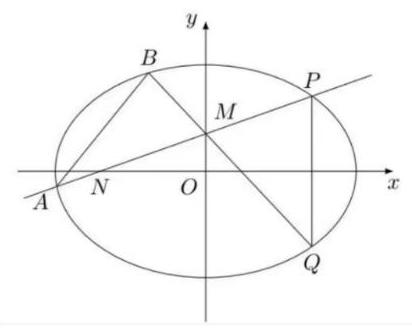
\includegraphics[max width=0.3\textwidth]{images/bo_d6dceus601uc73dvofhg_73_973_1380_412_329_0.jpg}
\end{center}
\hspace*{3em} 

【答案】(1) \(a = 2\sqrt{2}\) (2) \(a = \sqrt{3}\) (3) \({k}_{AB} = \frac{\sqrt{6}}{2}\)

【解析】(1) 由 \(\frac{c}{a} = \frac{\sqrt{3}}{2}\) ,可得 \(\frac{3}{4} = \frac{{c}^{2}}{{a}^{2}} = \frac{{a}^{2} - {b}^{2}}{{a}^{2}} = 1 - \frac{2}{{a}^{2}}\) ,所以 \({a}^{2} = 8\) ,即 \(a = 2\sqrt{2},4\) 分

(2)设 \(P\left( {{x}_{0},{y}_{0}}\right)\) ， \(N\left( {{x}_{n},0}\right)\) 则 \(Q\left( {{x}_{0}, - {y}_{0}}\right)\) ，

又 \(M\left( {0,\frac{\sqrt{3}}{3}}\right)\) 为线段 \({PN}\) 的中点,所以 \({y}_{0} = \frac{2\sqrt{3}}{3},6\) 分

又 \({MQ} \bot  {MP}\) 可得: \({x}_{0}^{2} + \frac{\sqrt{3}}{3}\left( {-\sqrt{3}}\right)  = 0\) ,即 \({x}_{0}^{2} = 1,8\) 分

又点 \(P\) 在椭圆 \(C\) 上，所以 \(\frac{1}{{a}^{2}} + \frac{2}{3} = 1\) ，所以 \({a}^{2} = 3\) ，即 \(a = \sqrt{3}\) ，10 分

(3)设 \(P\left( {{x}_{0},{y}_{0}}\right) ,{x}_{0},{y}_{0} > 0\) ，则 \(M\left( {0,\frac{{y}_{0}}{2}}\right) ,Q\left( {{x}_{0}, - {y}_{0}}\right)\) .

因为 \(\overrightarrow{QM} = 2\overrightarrow{MB}\) ,所以 \(B\left( {-\frac{{x}_{0}}{2},\frac{5{y}_{0}}{4}}\right) ,{12}\) 分

\(B,Q\) 代入椭圆方程 \(\left\{  \begin{array}{l} {x}_{0}^{2} + 2{y}_{0}^{2} = 4 \\  \frac{{x}_{0}^{2}}{4} + \frac{{50}{y}_{0}^{2}}{16} = 4 \end{array}\right.\) ,解得 \(\left\{  \begin{array}{l} {x}_{0} = \frac{2\sqrt{21}}{7} \\  {y}_{0} = \frac{2\sqrt{14}}{7} \end{array}\right.\) ,14 分

所以 \(P\left( {\frac{2\sqrt{21}}{7},\frac{2\sqrt{14}}{7}}\right) ,M\left( {0,\frac{\sqrt{14}}{7}}\right) ,B\left( {-\frac{\sqrt{21}}{7},\frac{5\sqrt{14}}{14}}\right) ,{MP} : y = \frac{\sqrt{6}}{6}x + \frac{\sqrt{14}}{7}\)

联立 \(\left\{  \begin{matrix} y = \frac{\sqrt{6}}{6}x + \frac{\sqrt{14}}{7} \\  {x}^{2} + 2{y}^{2} = 4 \end{matrix}\right. ,7{x}^{2} + \sqrt{21}x - {18} = 0\) ,则 \(A\left( {-\frac{3\sqrt{21}}{7}, - \frac{\sqrt{14}}{14}}\right)\) . 16 分

所以 \({k}_{AB} = \frac{\sqrt{6}}{2}\) . 18 分

7.【2025.12 虹口高三一模 20】已知椭圆 \(\Gamma  : \frac{{x}^{2}}{2} + {y}^{2} = 1\) 的左、右焦点分别为 \({F}_{1}\) 和 \({F}_{2}\) ,点 \(P\) 是 \(\Gamma\) 的长轴上的动点,点 \(Q\) 为 \(\Gamma\) 上的动点,且异于点 \(P\) .

(1)当点 \(P\) 位于椭圆 \(\Gamma\) 的左焦点，且 \(Q\) 、 \(P\) 、 \({F}_{2}\) 能构成三角形时，求 \({\Delta QP}{F}_{2}\) 的周长；

(2)当点 \(P\) 位于椭圆 \(\Gamma\) 的左顶点时,直线 \({PQ}\) 与 \(y\) 轴交于点 \(B\left( {0,\frac{1}{2}}\right) ,\overrightarrow{PB} = \lambda \overrightarrow{BQ}\) ，求实数 \(\lambda\) 的值:

(3)当点 \(P\) 与椭圆 \(\Gamma\) 的左、右顶点均不重合时，记直线 \({PQ}\) 与椭圆 \(\Gamma\) 的另一个交点为 \(S\) ，过点 \(P\) 作直线 \(l\) 与椭圆 \(\Gamma\) 交于 \(C\) 、 \(D\) 两点，设 \(M\) 和 \(N\) 分别为弦 \({QS}\) 和弦 \({CD}\) 的中点，若 \(P\) 、 \(Q\) 、 \(M\) 、 \(N\) 为四个相异的点， \(\left| {\overrightarrow{PM} + \overrightarrow{PN}}\right|  = \left| \overrightarrow{MN}\right|\) ，且直线 \({MN}\) 恒过定点 \(\left( {-\frac{1}{3},0}\right)\) ，求点 \(P\) 的坐标.

【答案】(1) \(2 + 2\sqrt{2}\) (2) \(\frac{5}{3}\) (3) \(\left( {-\frac{1}{2},0}\right)\)

【解析】(1) \({c}^{2} = {a}^{2} - {b}^{2} = 1\) ,故 \(c = 1\) . 2 分

\({\Delta QP}{F}_{2}\) 的周长为 \({2a} + {2c} = 2\sqrt{2} + 2\) . 4 分

(2) \(P\left( {-\sqrt{2},0}\right) ,B\left( {0,\frac{1}{2}}\right)\) ，所以直线 \({PB}\) 的方程为 \(y = \frac{\sqrt{2}}{4}x + \frac{1}{2}\) . 6 分 \(\left\{  \begin{array}{l} y = \frac{\sqrt{2}}{4}x + \frac{1}{2}, \\  \Gamma  : \frac{{x}^{2}}{2} + {y}^{2} = 1, \end{array}\right.\) 解得 \(Q\) 点的横坐标为 \(\frac{3}{5}\sqrt{2}\) . 8 分

所以 \(0 - \left( {-\sqrt{2}}\right)  = \lambda \left( {\frac{3}{5}\sqrt{2} - 0}\right)\) ,解得 \(\lambda  = \frac{5}{3}\) . 10 分

(3) \(\left| {\overrightarrow{PM} + \overrightarrow{PN}}\right|  = \left| \overrightarrow{MN}\right|\) ，故 \(\left| {\overrightarrow{PM} + \overrightarrow{PN}}\right|  = \left| {\overrightarrow{PN} - \overrightarrow{PM}}\right|\) ，即 \({PM}\bot {PN}\) . 12 分

设 \(P\left( {m,0}\right)\) ,由题,直线 \({QS}\) 和直线 \({CD}\) 均不与坐标轴垂直,设直线 \({QS}\) 的方程为 \(y = k\left( {x - m}\right)\) ,

且 \(m \neq  0\) . 设 \(S\left( {{x}_{1},{y}_{1}}\right) ,Q\left( {{x}_{2},{y}_{2}}\right) .\left\{  \begin{array}{l} y = k\left( {x - m}\right) , \\  {x}^{2} + 2{y}^{2} = 2, \end{array}\right.\) 解得 \(\left( {1 + 2{k}^{2}}\right) {x}^{2} - {4m}{k}^{2}x + 2{k}^{2}{m}^{2} - 2 = 0\) ,

则 \({x}_{1} + {x}_{2} = \frac{{4m}{k}^{2}}{1 + 2{k}^{2}}\) ,故 \(M\left( {\frac{{2m}{k}^{2}}{1 + 2{k}^{2}},\frac{-{mk}}{1 + 2{k}^{2}}}\right) ,N\left( {\frac{2m}{{k}^{2} + 2},\frac{mk}{{k}^{2} + 2}}\right)\) . 14 分

\({k}_{MN} = \frac{\frac{mk}{{k}^{2} + 2} - \frac{-{mk}}{1 + 2{k}^{2}}}{\frac{2m}{{k}^{2} + 2} - \frac{{2m}{k}^{2}}{1 + 2{k}^{2}}} = \frac{3k}{2\left( {1 - {k}^{2}}\right) }.\;{16}\) 分

当 \(k \neq   \pm  1\) 时,则直线 \({MN}\) 的直线方程为 \(y - \frac{mk}{{k}^{2} + 2} = \frac{3k}{2\left( {1 - {k}^{2}}\right) }\left( {x - \frac{2m}{{k}^{2} + 2}}\right)\) ,代入 \(\left( {-\frac{1}{3},0}\right)\) ,化简

得 \(- {mk} + m{k}^{3} =  - \frac{1}{2}{k}^{3} - k - {3mk}\) 恒成立,故 \(\left\{  \begin{array}{l} m =  - \frac{1}{2}, \\   - m =  - 1 - {3m}, \end{array}\right.\) 解得 \(m =  - \frac{1}{2}\) . 18 分

当 \(k =  \pm  1\) 时,则直线 \({MN}\) 的直线方程为 \(x = \frac{2}{3}m\) ,代入 \(\left( {-\frac{1}{3},0}\right)\) ,解得 \(m =  - \frac{1}{2}\) . 故 \(P\left( {-\frac{1}{2},0}\right)\) .

8.【2025.12 崇明高三一模 20】已知椭圆 \(\Gamma  : \frac{{x}^{2}}{2} + {y}^{2} = 1,{F}_{1}\text{ 、 }{F}_{2}\) 分别是 \(\Gamma\) 的左右焦点. 点 \(A\) 、 \(B\text{ 、 }C\text{ 、 }D\) 均在 \(\Gamma\) 上,且点 \(A\) 是第一象限点. 直线 \({AB}\) 经过点 \({F}_{1}\) ,直线 \({AC}\text{ 、 }{BD}\) 均经过点 \({F}_{2}\) .

(1)求椭圆 \(\Gamma\) 的离心率；

(2)若 \(\overrightarrow{{F}_{1}A} \cdot  \overrightarrow{{F}_{2}A} = \frac{1}{2}\) ，直线 \({AB}\) 的方程；

(3)求证: \(\frac{{k}_{CD}}{{k}_{AB}}\) 为定值.

【答案】(1) \(\frac{\sqrt{2}}{2}\) (2) \(y = \frac{\sqrt{2}}{4}\left( {x + 1}\right)\) (3)证明见解析，定值为 5

【解析】(1) \(c = \sqrt{{a}^{2} - {b}^{2}} = 1\) ,所以 \(e = \frac{c}{a} = \frac{\sqrt{2}}{2}\) .4 分

(2)由题意， \({F}_{1}\left( {-1,0}\right)\) ， \({F}_{2}\left( {1,0}\right)\) ，设 \(A\left( {x,y}\right) \left( {x > 0,y > 0}\right)\)

则 \(\overrightarrow{{F}_{1}A} \cdot  \overrightarrow{{F}_{2}A} = \left( {x + 1,y}\right)  \cdot  \left( {x - 1,y}\right)  = {x}^{2} - 1 + {y}^{2} = \frac{{x}^{2}}{2} = \frac{1}{2}\) ,所以 \(x = 1\) .2 分

故 \(A\left( {1,\frac{\sqrt{2}}{2}}\right) ,\;{k}_{AB} = \frac{\frac{\sqrt{2}}{2}}{1 - \left( {-1}\right) } = \frac{\sqrt{2}}{4}\) .4 分

故直线 \({AB}\) 的方程是 \(y = \frac{\sqrt{2}}{4}\left( {x + 1}\right)\) .6 分

(3)设 \(A\left( {{x}_{1},{y}_{1}}\right) ,B\left( {{x}_{2},{y}_{2}}\right) ,C\left( {{x}_{3},{y}_{3}}\right) ,D\left( {{x}_{4},{y}_{4}}\right)\) 则直线 \({AC}\) 方程为 \(x = {ty} + 1\) ，其中 \(t = \frac{{x}_{1} - 1}{{y}_{1}}\) 由 \(\left\{  \begin{array}{l} \frac{{x}^{2}}{2} + {y}^{2} = 1 \\  x = {ty} + 1 \end{array}\right.\) ,得: \(\left( {{t}^{2} + 2}\right) {y}^{2} + {2ty} - 1 = 0\)

故 \({y}_{1}{y}_{3} =  - \frac{1}{{t}^{2} + 2} =  - \frac{1}{{\left( \frac{{x}_{1} - 1}{{y}_{1}}\right) }^{2} + 2} =  - \frac{{y}_{1}^{2}}{{x}_{1}^{2} - 2{x}_{1} + 1 + 2{y}_{1}^{2}} = \frac{{y}_{1}^{2}}{2{x}_{1} - 3}\)

所以 \({y}_{3} = \frac{{y}_{1}}{2{x}_{1} - 3},{x}_{3} = t{y}_{3} + 1 = \frac{{x}_{1} - 1}{2{x}_{1} - 3} + 1\)

同理: \({y}_{4} = \frac{{y}_{2}}{2{x}_{2} - 3},{x}_{4} = t{y}_{4} + 1 = \frac{{x}_{2} - 1}{2{x}_{2} - 3} + 1\) .4 分

故 \({k}_{CD} = \frac{{y}_{4} - {y}_{3}}{{x}_{4} - {x}_{3}} = \frac{\frac{{y}_{2}}{2{x}_{2} - 3} - \frac{{y}_{1}}{2{x}_{1} - 3}}{\frac{3{x}_{2} - 4}{2{x}_{2} - 3} - \frac{3{x}_{1} - 4}{2{x}_{1} - 3}} = \frac{{y}_{2}\left( {2{x}_{1} - 3}\right)  - {y}_{1}\left( {2{x}_{2} - 3}\right) }{{x}_{1} - {x}_{2}}\) .6 分

设直线 \({AB}\) 方程为 \(y = k\left( {x + 1}\right)\) ,则 \({k}_{CD} = \frac{k\left( {{x}_{2} + 1}\right) \left( {2{x}_{1} - 3}\right)  - k\left( {{x}_{1} + 1}\right) \left( {2{x}_{2} - 3}\right) }{{x}_{1} - {x}_{2}} = {5k}\)

所以 \(\frac{{k}_{CD}}{{k}_{AB}} = 5\) ,为定值. .8 分

9.【2025.12 奉贤高三一模 20】椭圆 \(\frac{{x}^{2}}{{a}^{2}} + \frac{{y}^{2}}{{b}^{2}} = 1\left( {a > b > 0}\right)\) ， \(P\) 是第一象限内椭圆上的点， \({A}_{1}\left( {-a,0}\right) ,{B}_{1}\left( {0,b}\right) ,\left| {{A}_{1}{B}_{1}}\right|  = \sqrt{5}\) ,椭圆的离心率是 \(\frac{\sqrt{3}}{2}.M\left( {-t,0}\right) ,N\left( {t,0}\right) ,t > 0\) 且 \(t \neq  a\) .

(1)求椭圆的方程并在下图 1 中作出椭圆的左焦点，写出作图依据；

(2)如图 2，设 \(t = 1\) ，三角形 \({PMN}\) 的面积记为 \({S}_{1}\) ，三角形 \(P{A}_{1}{B}_{1}\) 的面积记为 \({S}_{2}\) ，若 \({S}_{2} = 2{S}_{1}\) ， 求点 \(P\) 的坐标;

(3)设 \(P\left( {{x}_{0},{y}_{0}}\right)\) ，连结 \({PM}\) 与椭圆交于点 \(A\) ，连结 \({PN}\) 与椭圆交于点 \(B\) ，判断 \(\frac{\left| PM\right| }{\left| MA\right| } + \frac{\left| PN\right| }{\left| NB\right| }\) 是否为定值? 请说明理由.

\begin{center}
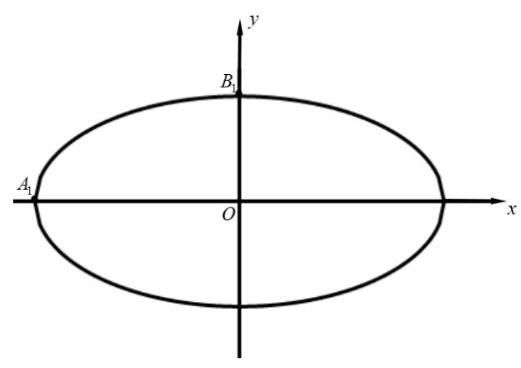
\includegraphics[max width=0.4\textwidth]{images/bo_d6dceus601uc73dvofhg_77_328_185_521_368_0.jpg}
\end{center}
\hspace*{3em} 

第 20 题图 1

\begin{center}
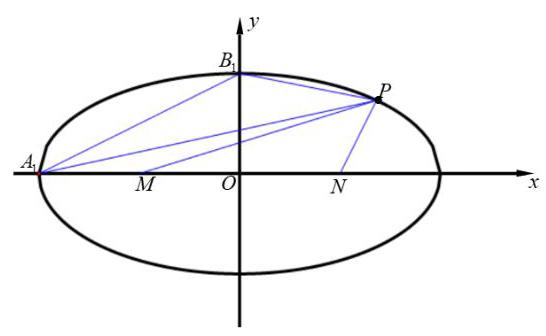
\includegraphics[max width=0.4\textwidth]{images/bo_d6dceus601uc73dvofhg_77_860_216_546_336_0.jpg}
\end{center}
\hspace*{3em} 

第 20 题图 2

\begin{center}
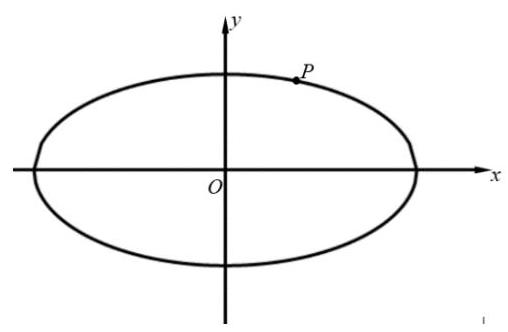
\includegraphics[max width=0.4\textwidth]{images/bo_d6dceus601uc73dvofhg_77_326_746_508_332_0.jpg}
\end{center}
\hspace*{3em} 

第 20 题图 3

\begin{center}
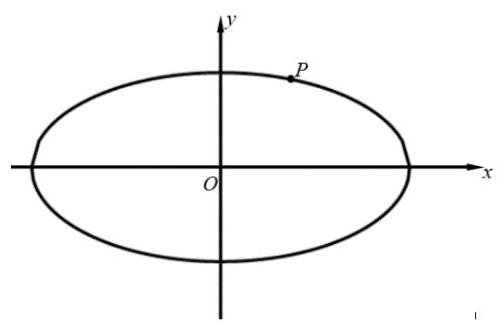
\includegraphics[max width=0.4\textwidth]{images/bo_d6dceus601uc73dvofhg_77_901_751_500_329_0.jpg}
\end{center}
\hspace*{3em} 

第 20 题(备用图)

【答案】(1)见解析

(2) \(P\left( {\frac{8}{5},\frac{4}{5}}\right)\) (3)是，定值为 \(\left| \frac{8 + 2{t}^{2}}{4 - {t}^{2}}\right|\)

【解析】(1) 已知 \({A}_{1}\left( {-a,0}\right) ,{B}_{1}\left( {0,b}\right)\) ,则 \(\left| {{A}_{1}{B}_{1}}\right|  = \sqrt{{a}^{2} + {b}^{2}} = \sqrt{5}\) ,

椭圆离心率 \(e = \frac{c}{a} = \frac{\sqrt{3}}{2}\) ，且 \({a}^{2} = {b}^{2} + {c}^{2}\) ，得 \(\left\{  \begin{array}{l} {a}^{2} = 4 \\  {b}^{2} = 1 \\  {c}^{2} = 3 \end{array}\right.\) ，椭圆方程 \(\frac{{x}^{2}}{4} + {y}^{2} = 1\)

作图依据: 以 \({B}_{1}\) 为圆心, \(O{A}_{1}\) 长为半径作圆,与 \(x\) 轴负半轴焦点即为左焦点.

(2)当 \(t = 1\) 时， \(M\left( {-1,0}\right)\) ， \(N\left( {1,0}\right)\) ， \({A}_{1}\left( {-2,0}\right)\) ， \({B}_{1}\left( {0,1}\right)\)

设 \(P\left( {{x}_{0},{y}_{0}}\right) \left( {{x}_{0} > 0,{y}_{0} > 0}\right)\) ,则 \(\frac{{x}_{0}{}^{2}}{4} + {y}_{0}^{2} = 1,{S}_{1} = \frac{1}{2}\left| {MN}\right| \left| {y}_{0}\right|  = {y}_{0}\) ( \(P\) 点第一象限)

直线 \({A}_{1}{B}_{1}\) 方程: \(x - {2y} + 2 = 0\) ，

\(P\) 到直线 \({A}_{1}{B}_{1}\) 距离 \(d = \frac{\left| {x}_{0} - 2{y}_{0} + 2\right| }{\sqrt{5}} = \frac{{x}_{0} - 2{y}_{0} + 2}{\sqrt{5}}\) ， \(\left( P\right.\) 点第一象限 \()\)

\({S}_{2} = \frac{1}{2}\left| {{A}_{1}{B}_{1}}\right|  \cdot  d = \frac{1}{2} \times  \sqrt{5} \times  \frac{{x}_{0} - 2{y}_{0} + 2}{\sqrt{5}} = \frac{{x}_{0} - 2{y}_{0} + 2}{2}\) ,

由 \({S}_{2} = 2{S}_{1}\) ,得 \(\frac{{x}_{0} - 2{y}_{0} + 2}{2} = 2{y}_{0}\) ,即 \({x}_{0} = 6{y}_{0} - 2\) ,

代入椭圆方程 \(\frac{{\left( 6{y}_{0} - 2\right) }^{2}}{4} + {y}_{0}^{2} = 1\) ,得故 \(P\left( {\frac{8}{5},\frac{3}{5}}\right)\) .

(3)当 \(M\text{ 、 }N\) 在椭圆内部，即 \(0 < t < 2\) ，设直线 \({PM}\) 的方程为 \(x = {my} - t\)

联立 \(\left\{  {\begin{array}{l} x = {my} - t \\  \frac{{x}^{2}}{4} + {y}^{2} = 1 \end{array}\therefore \left( {{m}^{2} + 4}\right) {y}^{2} - {2my} + {t}^{2} - 4 = 0}\right.\) ,

\({y}_{0}{y}_{A} = \frac{{t}^{2} - 4}{{m}^{2} + 4},\therefore {y}_{A} = \frac{{t}^{2} - 4}{{y}_{0}\left( {{m}^{2} + 4}\right) },\;\therefore \frac{\left| PM\right| }{\left| MA\right| } = \left| \frac{{y}_{0}}{{y}_{A}}\right|  = \frac{{y}_{0}{}^{2}\left( {{m}^{2} + 4}\right) }{4 - {t}^{2}}\) ,

\(\frac{\left| PM\right| }{\left| MA\right| } = \left| \frac{{y}_{0}}{{y}_{A}}\right|  = \frac{{y}_{0}^{2}\left( {{\left( \frac{{x}_{0} + t}{{y}_{0}}\right) }^{2} + 4}\right) }{4 - {t}^{2}} = \frac{4 + {t}^{2} + {2x}{t}_{0}}{4 - {t}^{2}}\) ,同法: \(\frac{\left| PN\right| }{\left| NB\right| } = \left| \frac{{y}_{0}}{{y}_{B}}\right|  = \frac{4 + {t}^{2} - {2x}{t}_{0}}{4 - {t}^{2}}\)

\(\frac{\left| PM\right| }{\left| MA\right| } + \frac{\left| PN\right| }{\left| NB\right| } = \frac{8 + 2{t}^{2}}{4 - {t}^{2}}\) 是定值，与点 \(P\) 无关

当 \(M\text{ 、 }N\) 在椭圆外部,即 \(2 < t\) ,

\(\frac{\left| PM\right| }{\left| MA\right| } + \frac{\left| PN\right| }{\left| NB\right| } = \frac{4 + {t}^{2} + {2x}{t}_{0}}{{t}^{2} - 4} + \frac{4 + {t}^{2} - {2x}{t}_{0}}{{t}^{2} - 4} = \frac{8 + 2{t}^{2}}{{t}^{2} - 4}\) 是定值，与点 \(P\) 无关。

10.【2025.12 普陀高三一模 20】设 \(a > 2,m \in  \mathbf{R},k\text{ 、 }t\) 是不全为零的实数，椭圆 \(\Gamma  : \frac{{x}^{2}}{{a}^{2}} + \frac{{y}^{2}}{4} = 1,{F}_{1}\text{ 、 }{F}_{2}\) 分别为 \(\Gamma\) 的左、右两个焦点,直线 \(l : {kx} + {ty} + m = 0\) 与 \(\Gamma\) 交于 \(A\text{ 、 }B\) 两点, \(O\) 为坐标原点.

(1)若 \(k = 0\) ， \(t + m = 0\) ，且四边形 \({AB}{F}_{1}{F}_{2}\) 为矩形，求 \(\Gamma\) 的离心率；

(2)若 \(t = 0\) ，且 \(\Delta {F}_{1}{AB}\) 的周长的最大值为12，求 \(\Gamma\) 的方程；

(3)若 \(a = 4,t =  - 1,\lambda  > 0\) ，直线 \({OA}\) 与 \({OB}\) 的斜率之积为 \(- \frac{1}{4},C\) 为 \({OA}\) 上的一点，且 \(\overrightarrow{OA} = \overrightarrow{AC}\) ,直线 \({BC}\) 与椭圆 \(\Gamma\) 交于点 \(D\) ,且 \(\overrightarrow{BD} = \lambda \overrightarrow{DC}\) ,求 \(\lambda\) 的值以及 \({\Delta ADB}\) 的面积 \(S\) 的值.

【答案】( 1 ) \(e = \frac{c}{a} = \frac{\sqrt{3}}{2}\) (2) \(\Gamma  : \frac{{x}^{2}}{9} + \frac{{y}^{2}}{4} = 1\) (3) \({S}_{\Delta ABD} = \frac{2}{5}{S}_{\Delta OAB} = \frac{8}{5}\)

【解析】(1) 由 \(k = 0,t + m = 0\) 得, \(l : y = 1\) ,由 \(\frac{{x}^{2}}{{a}^{2}} + \frac{1}{4} = 1\) ,解得 \(x =  \pm  \frac{\sqrt{3}}{2}a,\ldots \ldots 2\) 分又四边形 \({AB}{F}_{1}{F}_{2}\) 是矩形,则 \(\frac{\sqrt{3}}{2}a = c\) ,即离心率 \(e = \frac{c}{a} = \frac{\sqrt{3}}{2}\) . .4 分

(2)由 \(t = 0\) 得, \(l : x =  - \frac{m}{k}\) ，即 \({AB}\bot x\) 轴， .1 分则 \(A{F}_{1} + B{F}_{1} + {AB} \leq  A{F}_{1} + B{F}_{1} + A{F}_{2} + B{F}_{2} = {4a}\) , .4 分且等号当且仅当 \({AB}\) 过右焦点 \({F}_{2}\) 时取得,即 \(\Delta {F}_{1}{AB}\) 的周长的最大值为 \({4a}\) , 即 \({4a} = {12}\) ,即 \(a = 3\) ,则所求的 \(\Gamma  : \frac{{x}^{2}}{9} + \frac{{y}^{2}}{4} = 1\) . .6 分

(3)设 \(A\left( {{x}_{1},{y}_{1}}\right)\) ， \(B\left( {{x}_{2},{y}_{2}}\right)\) ， \(D\left( {{x}_{0},{y}_{0}}\right)\) ，由 \(\overrightarrow{OA} = \overrightarrow{AC}\) 得，点 \(C\left( {2{x}_{1},2{y}_{1}}\right)\) ，

又 \(\overrightarrow{BD} = \lambda \overrightarrow{DC}\) ,则 \({x}_{0} = \frac{{x}_{2} + \lambda  \cdot  2{x}_{1}}{1 + \lambda },{y}_{0} = \frac{{y}_{2} + \lambda  \cdot  2{y}_{1}}{1 + \lambda }\) ,

因为点 \(D\) 在 \(\Gamma\) 上,所以 \(\frac{{\left( \frac{{x}_{2} + \lambda  \cdot  2{x}_{1}}{1 + \lambda }\right) }^{2}}{16} + \frac{{\left( \frac{{y}_{2} + \lambda  \cdot  2{y}_{1}}{1 + \lambda }\right) }^{2}}{4} = 1\)

则 \(4{\lambda }^{2}\left( {\frac{{x}_{1}^{2}}{16} + \frac{{y}_{1}^{2}}{4}}\right)  + \left( {\frac{{x}_{2}^{2}}{16} + \frac{{y}_{2}^{2}}{4}}\right)  + \frac{\lambda }{4}\left( {{x}_{1}{x}_{2} + 4{y}_{1}{y}_{2}}\right)  = {\left( 1 + \lambda \right) }^{2}\) ,

又点 \(A\text{ 、 }B\) 均在 \(\Gamma\) 上,则 \(\frac{{x}_{1}^{2}}{16} + \frac{{y}_{1}^{2}}{4} = 1,\frac{{x}_{2}^{2}}{16} + \frac{{y}_{2}^{2}}{4} = 1\) ,

由 \({k}_{OA} \cdot  {k}_{OB} =  - \frac{1}{4}\) 得, \(\frac{{y}_{1}{y}_{2}}{{x}_{1}{x}_{2}} =  - \frac{1}{4}\) ,即 \({x}_{1}{x}_{2} + 4{y}_{1}{y}_{2} = 0\) ,

则 \(4{\lambda }^{2} + 1 = {\left( 1 + \lambda \right) }^{2}\) ，又 \(\lambda  > 0\) ，即 \(\lambda  = \frac{2}{3}\) . .3 分

由 \(\overrightarrow{BD} = \frac{2}{3}\overrightarrow{DC},\overrightarrow{OA} = \overrightarrow{AC}\) 得, \({S}_{\bigtriangleup {ABD}} = \frac{2}{5}{S}_{\bigtriangleup {ABC}} = \frac{2}{5}{S}_{\bigtriangleup {OAB}}\) , .4 分

又 \(a = 4,t =  - 1\) ,即直线 \(l : y = {kx} + m\) ,

由 \(\left\{  \begin{matrix} y = {kx} + m \\  \frac{{x}^{2}}{16} + \frac{{y}^{2}}{4} = 1 \end{matrix}\right.\) 得, \(\left( {1 + 4{k}^{2}}\right) {x}^{2} + {8kmx} + 4{m}^{2} - {16} = 0\) ,

则 \({x}_{1} + {x}_{2} = \frac{-{8km}}{1 + 4{k}^{2}},{x}_{1}{x}_{2} = \frac{4{m}^{2} - {16}}{1 + 4{k}^{2}}\) ,

则 \(\left| {AB}\right|  = \sqrt{1 + {k}^{2}}\left| {{x}_{1} - {x}_{2}}\right|  = \sqrt{1 + {k}^{2}}\sqrt{{\left( {x}_{1} + {x}_{2}\right) }^{2} - 4{x}_{1}{x}_{2}}\)

\(= \sqrt{1 + {k}^{2}}\sqrt{{\left( \frac{-{8km}}{1 + 4{k}^{2}}\right) }^{2} - 4 \cdot  \frac{4{m}^{2} - {16}}{1 + 4{k}^{2}}} = \frac{4\sqrt{1 + {k}^{2}}}{1 + 4{k}^{2}}\sqrt{4 + {16}{k}^{2} - {m}^{2}}\)

由 \({x}_{1}{x}_{2} + 4{y}_{1}{y}_{2} = 0\) 得, \({x}_{1}{x}_{2} + 4{y}_{1}{y}_{2} = {x}_{1}{x}_{2} + 4\left( {k{x}_{1} + m}\right) \left( {k{x}_{2} + m}\right)  = 0\) ,

即 \(\left( {1 + 4{k}^{2}}\right) {x}_{1}{x}_{2} + {4km}\left( {{x}_{1} + {x}_{2}}\right)  + 4{m}^{2} = 0\) ,即 \(\left( {1 + 4{k}^{2}}\right) \frac{4{m}^{2} - {16}}{1 + 4{k}^{2}} - \frac{{32}{k}^{2}{m}^{2}}{1 + 4{k}^{2}} + 4{m}^{2} = 0\) ,

化简整理得, \({m}^{2} = 8{k}^{2} + 2\) ,则 \(\left| {AB}\right|  = \frac{4\sqrt{2\left( {1 + {k}^{2}}\right) }}{\sqrt{1 + 4{k}^{2}}}\) , .6 分

又原点 \(O\) 到直线 \(l\) 的距离为 \(d = \frac{\left| m\right| }{\sqrt{1 + {k}^{2}}} = \frac{\sqrt{2\left( {1 + 4{k}^{2}}\right) }}{\sqrt{1 + {k}^{2}}}\) ,

则 \({S}_{\bigtriangleup {OAB}} = \frac{1}{2} \times  \frac{4\sqrt{2\left( {1 + {k}^{2}}\right) }}{\sqrt{1 + 4{k}^{2}}} \times  \frac{\sqrt{2\left( {1 + 4{k}^{2}}\right) }}{\sqrt{1 + {k}^{2}}} = 4\) . 则 \({S}_{\bigtriangleup {ABD}} = \frac{2}{5}{S}_{\bigtriangleup {OAB}} = \frac{8}{5}\) . .8 分 \(\leq\)

11.【2025.12 青浦高三一模 20】已知椭圆 \(\Gamma  : \frac{{x}^{2}}{{a}^{2}} + \frac{{y}^{2}}{{a}^{2} - 4} = 1\left( {a > 2}\right)\) 的左、右焦点分别为 \({F}_{1}\text{ 、 }{F}_{2}\) ,

\(A\text{ 、 }B\) 为 \(\Gamma\) 上两个不同的点,记 \(\bigtriangleup {AB}{F}_{1}\) 的周长和面积分别为 \(C\) 和 \(S\) .

(1)若 \(\Gamma\) 的离心率为 \(\frac{1}{2}\) ，求 \(a\) 的值；

(2)若满足 \(\left| {A{F}_{1}}\right|  = {10}\) 的点 \(A\) 有且仅有两个，求 \(a\) 的取值范围；

(3)若 \(a = \sqrt{5}\) ，是否存在点 \(A\) 、 \(B\) 使得 \(C\) 和 \(S\) 同时取到最大值？若存在，求出直线 \({AB}\) 的方程; 若不存在, 说明理由.

【答案】(1) \(a = 4\) (2) \(8 < a < {12}\) (3)存在点 \(A\text{ 、 }B\) 使得 \(C\) 和 \(S\) 同时取到最大值 \(4\sqrt{5}\) 和 \(\sqrt{5}\) ,此时直线 \({AB}\) 的方程为 \(x \pm  \sqrt{3}y - 2 = 0\)

【解析】(1) 由条件知, \(\frac{2}{a} = \frac{1}{2},\therefore a = 4\) .

(2)由条件知， \({F}_{1}\left( {-2,0}\right)\) ，设点 \(A\left( {x,y}\right)\) ，则 \(\left| {AF}\right|  = \sqrt{{\left( x + 2\right) }^{2} + {y}^{2}}\)

\(= \sqrt{{\left( x + 2\right) }^{2} + \frac{{a}^{2}\left( {{a}^{2} - 4}\right)  - \left( {{a}^{2} - 4}\right) {x}^{2}}{{a}^{2}}} = \sqrt{\frac{4{x}^{2} + 4{a}^{2}x + {a}^{4}}{{a}^{2}}} = \left| {a + \frac{2}{a}x}\right|\)

当且仅当 \(- a < x < a\) ,即点 \(A\) 不取左右顶点时, \(y\) 有两个解,因此只需 \(a - 2 < {10} < a + 2\) , \(\therefore 8 < a < {12}\) .

(3) \(C = \left| {A{F}_{1}}\right|  + \left| {B{F}_{1}}\right|  + \left| {AB}\right|  \leq  \left| {A{F}_{1}}\right|  + \left| {B{F}_{1}}\right|  + \left| {A{F}_{2}}\right|  + \left| {B{F}_{2}}\right|  = 4\sqrt{5}\) ，当且仅当 \({F}_{2}\) 在弦 \({AB}\) 上时等号成立,此时 \(C\) 取到最大值 \(4\sqrt{5}\) .

设过点 \({F}_{2}\) 的直线 \({AB}\) 方程为 \(x = {ty} + 2\) (显然 \({AB}\) 斜率不为零),设 \(A\left( {{x}_{1},{y}_{1}}\right) ,B\left( {{x}_{2},{y}_{2}}\right)\) .

由 \(\left\{  \begin{matrix} x = {ty} + 2 \\  {x}^{2} + 5{y}^{2} = 5 \end{matrix}\right.\) 得 \(\left( {{t}^{2} + 5}\right) {y}^{2} + {4ty} - 1 = 0,\therefore \left\{  \begin{matrix} \Delta  = {20}\left( {{t}^{2} + 1}\right)  > 0 \\  {y}_{1} + {y}_{2} = \frac{-{4t}}{{t}^{2} + 5} \\  {y}_{1}{y}_{2} = \frac{-1}{{t}^{2} + 5} \end{matrix}\right.\) ,

\(S = \frac{1}{2}\left| {{F}_{1}{F}_{2}}\right|  \cdot  \left| {{y}_{1} - {y}_{2}}\right|  = \frac{4\sqrt{5}\sqrt{{t}^{2} + 1}}{{t}^{2} + 5} = \frac{4\sqrt{5}}{\sqrt{{t}^{2} + 1} + \frac{4}{\sqrt{{t}^{2} + 1}}} \leq  \sqrt{5}\) ,当且仅当 \(t =  \pm  \sqrt{3}\) 时等号成立,此时 \(S\) 取到最大值 \(\sqrt{5}\) .

综上所述,存在点 \(A\text{ 、 }B\) 使得 \(C\) 和 \(S\) 同时取到最大值 \(4\sqrt{5}\) 和 \(\sqrt{5}\) ,

此时直线 \({AB}\) 的方程为 \(x \pm  \sqrt{3}y - 2 = 0 >\)

12.【2025.12 浦东高三一模 20】已知椭圆 \(C : \frac{{x}^{2}}{9} + \frac{{y}^{2}}{8} = 1\) ,点 \(O\) 为坐标原点,椭圆的右顶点为 \(A\) ,左右焦点分别为 \({F}_{1}\text{ 、 }{F}_{2}\) ,点 \(E\) 为椭圆在 \(x\) 轴上方的一动点.

(1)求椭圆 \(C\) 的焦距与 \(\bigtriangleup E{F}_{1}{F}_{2}\) 的周长;

(2)若 \(\overrightarrow{EA} \cdot  \overrightarrow{E{F}_{1}} = \frac{9}{4}\) ，求点 \(E\) 到 \(x\) 轴的距离；

(3)过点 \({F}_{1}\) 作斜率为 \(k\) 的直线 \(l\) 交 \(y\) 轴正半轴于点 \(P\) ，点 \(P\) 位于椭圆内. 直线 \(l\) 与椭圆 \(C\) 交于 \(G\text{ 、 }H\) 两点,记 \(\bigtriangleup {OGH}\text{ 、 }\bigtriangleup O{F}_{1}P\) 的面积分别为 \({S}_{1}\text{ 、 }{S}_{2}\) ,求 \(\frac{{S}_{1}}{{S}_{2}}\) 的取值范围.

【答案】(1) \({2a} + {2c} = 8\) (2) \(\sqrt{6}\) (3) \(\left( {\frac{9}{5},6}\right)\)

【解析】(1) 由题意,椭圆的焦距 \({2c} = 2\sqrt{9 - 8} = 2\) , .2 分所以 \(\bigtriangleup E{F}_{1}{F}_{2}\) 的周长为 \({2a} + {2c} = 8\) .4 分

(2)由题， \(A\left( {3,0}\right)\) 、 \({F}_{1}\left( {-1,0}\right)\) ，设 \(E\left( {{x}_{0},{y}_{0}}\right)\) ，其中 \({y}_{0} > 0\) .

则 \(\overrightarrow{EA} = \left( {3 - {x}_{0}, - {y}_{0}}\right) \text{ 、 }\overrightarrow{E{F}_{1}} = \left( {-1 - {x}_{0}, - {y}_{0}}\right)\) , .6 分

\(\overrightarrow{EA} \cdot  \overrightarrow{E{F}_{1}} = \left( {3 - {x}_{0}}\right)  \cdot  \left( {-1 - {x}_{0}}\right)  = \frac{9}{4}\) .7 分

又点 \(E\) 在椭圆上,故 \(\frac{{x}_{0}^{2}}{9} + \frac{{y}_{0}^{2}}{8} = 1\)

联立方程,消 \({y}_{0}\) 可得 \({x}_{0}{}^{2} - 2{x}_{0} - 3 + 8\left( {1 - \frac{{x}_{0}}{9}}\right)  = \frac{9}{4}\) , .8 分即 \(\frac{1}{9}{x}_{0}{}^{2} - 2{x}_{0} + \frac{11}{4} = 0\) 解得 \(x = \frac{33}{2}\) (舍) 或 \(x = \frac{3}{2}\) , .9 分

代入椭圆，得 \({y}_{0} = \sqrt{6}\) ，即点 \(E\) 到 \(x\) 轴的距离为 \(\sqrt{6}\) 10 分

(3)由题意，直线 \(l\) 的方程为 \(y = k\left( {x + 1}\right) ,k \in  \left( {0,2\sqrt{2}}\right)\) .11 分设 \(G\left( {{x}_{1},{y}_{1}}\right) \text{ 、 }H\left( {{x}_{2},{y}_{2}}\right)\) ,联立方程 \(\left\{  \begin{array}{l} y = k\left( {x + 1}\right) \\  \frac{{x}^{2}}{9} + \frac{{y}^{2}}{8} = 1 \end{array}\right.\) ,

得 \(\left( {9{k}^{2} + 8}\right) {x}^{2} + {18}{k}^{2}x + 9{k}^{2} - {72} = 0\) , .12 分

则 \(\Delta  = {2304}{k}^{2} + {2304} > 0,{x}_{1} + {x}_{2} = \frac{-{18}{k}^{2}}{9{k}^{2} + 8},{x}_{1}{x}_{2} = \frac{9{k}^{2} - {72}}{9{k}^{2} + 8}\) .13 分

又 \(\frac{{S}_{1}}{{S}_{2}} = \frac{\left| GH\right| }{\left| {F}_{1}P\right| } = \frac{\left| {x}_{1} - {x}_{2}\right| }{1}\) 14 分

\(= \sqrt{{\left( {x}_{1} + {x}_{2}\right) }^{2} - 4{x}_{1}{x}_{2}} = \frac{{48}\sqrt{{k}^{2} + 1}}{9{k}^{2} + 8}\) .16 分

令 \(\sqrt{{k}^{2} + 1} = t\) ,则 \(t \in  \left( {1,3}\right)\) ,因而 \(\frac{{S}_{1}}{{S}_{2}} = \frac{48t}{9{t}^{2} - 1} = \frac{48}{{9t} - \frac{1}{t}}\) , .17 分

又 \(y = \frac{48}{{9t} - \frac{1}{t}}\) 在 \(t \in  \left( {1,3}\right)\) 上严格递减,故 \(\frac{{S}_{1}}{{S}_{2}}\) 的取值范围为 \(\left( {\frac{9}{5},6}\right)\) .18 分

13.【2025.12 金山高三一模 20】已知椭圆 \(\Gamma  : \frac{{x}^{2}}{16} + \frac{{y}^{2}}{4} = 1\) ，点 \(O\) 为坐标原点，点 \(M\) 为椭圆 \(\Gamma\) 上一点.

(1)求椭圆 \(\Gamma\) 的离心率；

(2)已知点 \({F}_{2}\) 为椭圆 \(\Gamma\) 的右焦点，直线 \({l}_{0} : x = \frac{8\sqrt{3}}{3}\) ，证明:点 \(M\) 到点 \({F}_{2}\) 的距离与到直线 \({l}_{0}\) 的距离之比为定值;

(3)过线段 \({OM}\) 中点 \(N\) 的直线 \(l\) 交椭圆 \(\Gamma\) 于 \(P\) 、 \(Q\) 两点，求 \({S}_{\Delta PMQ}\) 的最大值.

\begin{center}
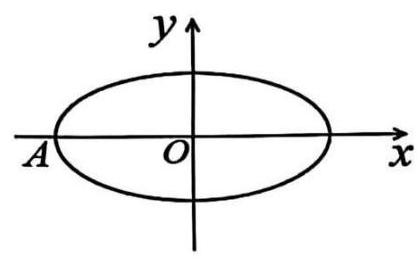
\includegraphics[max width=0.3\textwidth]{images/bo_d6dceus601uc73dvofhg_82_983_1802_419_261_0.jpg}
\end{center}
\hspace*{3em} 

【答案】(1) \(e = \frac{\sqrt{3}}{2}\) (3) \(2\sqrt{3}\)

【解析】(1) 因为 \(a = 4,b = 2\) , .1 分

所以 \({c}^{2} = {a}^{2} - {b}^{2} = {12}\) ,得 \(c = 2\sqrt{3}\) . .2 分

所以椭圆的离心率为 \(e = \frac{\sqrt{3}}{2}\) . .4 分

(2)设 \(M\left( {x,y}\right) \left( {-4 \leq  x \leq  4}\right)\) 所以 \(\left| {M{F}_{2}}\right|  = \sqrt{{\left( x - 2\sqrt{3}\right) }^{2} + {y}^{2}} = \sqrt{\frac{3}{4}{x}^{2} - 4\sqrt{3}x + {16}}\) . .6 分 \({d}_{{l}_{0}} = \frac{8\sqrt{3}}{3} - x.\) .8 分

所以 \(\frac{\left| M{F}_{2}\right| }{{d}_{{l}_{0}}} = \frac{\sqrt{\frac{3}{4}{x}^{2} - 4\sqrt{3}x + {16}}}{\frac{8\sqrt{3}}{3} - x} = \frac{\sqrt{3}}{2}\) . 10 分

(3)因为点 \(N\) 为线段 \({OM}\) 的中点，所以 \({S}_{\Delta PMQ} = {S}_{\Delta PQO}\) . 设 \(N\left( {m,n}\right)\) ，所以 \(M\left( {{2m},{2n}}\right)\) 因为 \(M\left( {{2m},{2n}}\right)\) 在椭圆 \(\Gamma\) 上,所以 \(\frac{{m}^{2}}{4} + {n}^{2} = 1\) .11 分

\({1}^{ \circ  }\) 当 \({k}_{PQ}\) 不存在时, \({l}_{PQ} : x = m, - 2 \leq  m \leq  2\left\{  \begin{matrix} x = m \\  \frac{{x}^{2}}{16} + \frac{{y}^{2}}{4} = 1 \end{matrix}\right.\) ,所以 \(y =  \pm  \frac{1}{2}\sqrt{{16} - {m}^{2}}\) ,

所以 \({S}_{\bigtriangleup {PMQ}} = {S}_{\bigtriangleup {PQO}} = \frac{1}{2}\sqrt{{16} - {m}^{2}} \times  \left| m\right|  = \frac{1}{2}\sqrt{-{\left( {m}^{2} - 8\right) }^{2} + {64}}\) . .12 分

所以当 \(m = 2\) 时， \({S}_{\Delta PMQ}\) 有最大值为 \(2\sqrt{3}\) . .13 分

\({2}^{ \circ  }\) 当 \({k}_{PQ}\) 存在时,设 \({l}_{PQ} : y = {kx} + b\)

\(\left\{  {\begin{matrix} y = {kx} + b \\  \frac{{x}^{2}}{16} + \frac{{y}^{2}}{4} = 1 \end{matrix} \Rightarrow  \left( {4{k}^{2} + 1}\right) {x}^{2} + {8kbx} + 4{b}^{2} - {16} = 0}\right.\) .14 分

此时, \(\Delta  =  - {16}\left( {{b}^{2} - {16}{k}^{2} - 4}\right)  > 0\) ,得: \({b}^{2} - {16}{k}^{2} - 4 < 0\) .

所以 \({S}_{\bigtriangleup {PMQ}} = {S}_{\bigtriangleup {POQ}} = \frac{1}{2}\left| {b\left| \cdot \right| {x}_{1} - {x}_{2}}\right|\)

\(= \frac{2\sqrt{-{b}^{4} + 4\left( {4{k}^{2} + 1}\right) {b}^{2}}}{4{k}^{2} + 1} = 2\sqrt{-{\left( \frac{{b}^{2}}{4{k}^{2} + 1}\right) }^{2} + 4\left( \frac{{b}^{2}}{4{k}^{2} + 1}\right) }\) .16 分

又因为点 \(N\) 落在直线 \({l}_{PQ}\) 上,所以 \(\left\{  {\begin{array}{l} n = {km} + b \\  \frac{{m}^{2}}{4} + {n}^{2} = 1 \end{array} \Rightarrow  \left( {4{k}^{2} + 1}\right) {m}^{2} + {8kbm} + 4{b}^{2} - 4 = 0}\right.\)

此时, \(\Delta  \geq  0\) ,得: \({b}^{2} \leq  4{k}^{2} + 1\) . .17 分

令 \(t = \frac{{b}^{2}}{4{k}^{2} + 1},0 < t \leq  1\) ,所以 \({S}_{\bigtriangleup {PMQ}} = 2\sqrt{-{t}^{2} + {4t}} = 2\sqrt{-{\left( t - 2\right) }^{2} + 4}\) .

当 \(t = 1\) ，即 \({b}^{2} = 4{k}^{2} + 1\) 时， \({S}_{\Delta PMQ}\) 有最大值为 \(2\sqrt{3}\) . .18 分

综上， \({S}_{\Delta PMQ}\) 有最大值为 \(2\sqrt{3}\) .

14.【2025.12 松江高三一模 20】已知椭圆 \(\frac{{x}^{2}}{{a}^{2}} + \frac{{y}^{2}}{{b}^{2}} = 1\left( {a > b > 0}\right)\) 的左焦点为 \(F\) ，过点 \(F\) 的直线交椭圆于 \(A,B\) 两点. \(\left| {AF}\right|\) 的最大值是 \(M,\left| {BF}\right|\) 的最小值是 \(m\) ,满足 \(M \cdot  m = \frac{3{a}^{2}}{4}\) .

(1)求该椭圆的离心率；

(2)若 \(a = 2\) ，点 \(P\) 在椭圆上，且在 \(x\) 轴上方，线段 \(\left| {PF}\right|\) 的中点 \(Q\) 在以原点 \(O\) 为圆心， \(\left| {OF}\right|\) 为半径的圆上,求直线 \({PF}\) 的斜率;

(3)设线段 \({AB}\) 的中点为 \(G,{AB}\) 的垂直平分线与 \(x\) 轴和 \(y\) 轴分别交于 \(D,E\) 两点， \(O\) 是坐标原点. 记 \({\Delta GFD}\) 的面积为 \({S}_{1},{\Delta OED}\) 的面积为 \({S}_{2}\) ,求 \(\frac{2{S}_{1}{S}_{2}}{{S}_{1}{}^{2} + {S}_{2}{}^{2}}\) 的取值范围.

【答案】(1) \(\frac{1}{2}\) (2) \(\sqrt{3}\)

(3) \(\left( {0,\frac{9}{41}}\right)\)

【解析】(1) \(\because M = a + c,m = a - c,\therefore M \cdot  m = \left( {a + c}\right)  \cdot  \left( {a - c}\right)  = {a}^{2} - {c}^{2} = \frac{3{a}^{2}}{4}\) , \(\therefore {c}^{2} = \frac{1}{4}{a}^{2},\therefore\) 离心率 \(e = \frac{c}{a} = \frac{1}{2}\) . 4 分

(2) \(\because a = 2,\therefore\) 椭圆方程为 \(\frac{{x}^{2}}{4} + \frac{{y}^{2}}{3} = 1,\therefore\) 左焦点 \(F\) 为(-1,0)，设右焦点为 \({F}_{1}\left( {1,0}\right)\) . \(\because \left| {OF}\right|  = \left| {OQ}\right|  = 1,\therefore \left| {P{F}_{1}}\right|  = 2\) . 设 \(P\) 点坐标为 \(\left( {x,y}\right)\) ,则 \(\left\{  \begin{array}{l} {\left( x - 1\right) }^{2} + {y}^{2} = 4 \\  \frac{{x}^{2}}{4} + \frac{{y}^{2}}{3} = 1 \end{array}\right.\) ,解得 \(x = 0\) 或 \(8\left( \text{ 舍 }\right)\) 从而 \(P\) 点坐标为 \(\left( {0,\sqrt{3}}\right) ,\therefore {k}_{PF} = \sqrt{3},\therefore\) 直线 \({PF}\) 的斜率为 \(\sqrt{3}\) . -10 分

(3)由(1)知， \(a = {2c}\) ， \(\therefore b = \sqrt{3}c\) ， \(\therefore\) 椭圆方程为 \(\frac{{x}^{2}}{4{c}^{2}} + \frac{{y}^{2}}{3{c}^{2}} = 1\) .

显然直线 \({AB}\) 的斜率存在且不为零,

设直线 \({AB}\) 的方程为 \(y = k\left( {x + c}\right)\) ,且 \(A\left( {{x}_{1},{y}_{1}}\right) ,B\left( {{x}_{2},{y}_{2}}\right)\) ,

则由 \(\left\{  \begin{array}{l} y = k\left( {x + c}\right) \\  \frac{{x}^{2}}{4{c}^{2}} + \frac{{y}^{2}}{3{c}^{2}} = 1 \end{array}\right.\) 消去 \(y\) 并整理得 \(\left( {4{k}^{2} + 3}\right) {x}^{2} + {8c}{k}^{2}x + 4{k}^{2}{c}^{2} - {12}{c}^{2} = 0\) ,

从而有 \({x}_{1} + {x}_{2} =  - \frac{{8c}{k}^{2}}{4{k}^{2} + 3},{y}_{1} + {y}_{2} = k\left( {{x}_{1} + {x}_{2} + {2c}}\right)  = \frac{6ck}{4{k}^{2} + 3}\) ,

所以 \(G\left( {-\frac{{4c}{k}^{2}}{4{k}^{2} + 3},\frac{3ck}{4{k}^{2} + 3}}\right)\) , -12 分

因为 \({DG} \bot  {AB}\) ,所以 \(\frac{\frac{3ck}{4{k}^{2} + 3}}{-\frac{{4c}{k}^{2}}{4{k}^{2} + 3} - {x}_{D}} \cdot  k =  - 1\) ,所以 \({x}_{D} = \frac{c{k}^{2}}{4{k}^{2} + 3}\) , -14 分由 \({Rt\Delta FGD}\) 与 \({Rt\Delta EOD}\) 相似,

所以 \(\frac{{S}_{1}}{{S}_{2}} = \frac{G{D}^{2}}{O{D}^{2}} = \frac{{\left( -\frac{{4c}{k}^{2}}{4{k}^{2} + 3} + \frac{c{k}^{2}}{4{k}^{2} + 3}\right) }^{2} + {\left( \frac{3ck}{4{k}^{2} + 3}\right) }^{2}}{{\left( -\frac{c{k}^{2}}{4{k}^{2} + 3}\right) }^{2}} = 9 + \frac{9}{{k}^{2}} > 9\) , -16 分令 \(\frac{{S}_{1}}{{S}_{2}} = t\) ,则 \(t > 9\) ,

从而 \(\frac{2{S}_{1}{S}_{2}}{{S}_{1}^{2} + {S}_{1}^{2}} = \frac{2}{t + \frac{1}{t}} < \frac{2}{9 + \frac{1}{9}} = \frac{9}{41}\) ,即 \(\frac{2{S}_{1}{S}_{2}}{{S}_{1}^{2} + {S}_{1}^{2}}\) 的取值范围为 \(\left( {0,\frac{9}{41}}\right)\) -18 分》

\section*{7.3 双曲线}

\section*{【知识梳理】}

\section*{1.双曲线的定义}

平面内到两个定点 \({F}_{1},{F}_{2}\) 的距离之差的绝对值等于常数 \({2a}\left( {0 < {2a} < \left| {{F}_{1}{F}_{2}}\right| }\right)\) 的点的轨迹叫做双曲线. 定点 \({F}_{1},{F}_{2}\) 叫做双曲线的焦点,两个焦点间的距离 \(\left| {{F}_{1}{F}_{2}}\right|\) 叫做双曲线的焦距.

若 \({2a} = \left| {{F}_{1}{F}_{2}}\right|\) ,则其轨迹为分别以 \({F}_{1},{F}_{2}\) 为端点不包括线段 \({F}_{1},{F}_{2}\) 的两条射线;

若 \({2a} > \left| {{F}_{1}{F}_{2}}\right|\) ,则其轨迹不存在;

还要注意定义中“绝对值”的条件也不可少. 因为仅满足 \(\left| {M{F}_{1}}\right|  - \left| {M{F}_{2}}\right|  = {2a}\) 的轨迹只是双曲线的一支.

\section*{2.双曲线的标准方程和几何性质}

\begin{center}
\adjustbox{max width=\textwidth}{
\begin{tabular}{|c|c|c|c|}
\hline
\phantom{X} & 标准方程 & \(\frac{{x}^{2}}{{a}^{2}} - \frac{{y}^{2}}{{b}^{2}} = 1\left( {a > 0,b > 0}\right)\) & \(\frac{{y}^{2}}{{a}^{2}} - \frac{{x}^{2}}{{b}^{2}} = 1\left( {a > 0,b > 0}\right)\) \\
\cline{1-4}
\multicolumn{2}{|c|}{图像} & 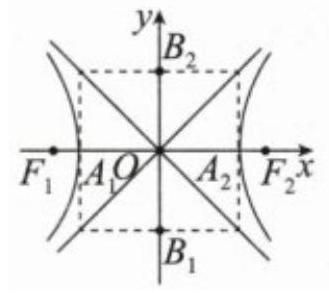
\includegraphics[max width=0.2\textwidth]{images/bo_d6dceus601uc73dvofhg_86_514_1098_329_293_0.jpg} & 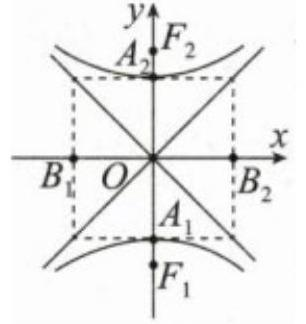
\includegraphics[max width=0.2\textwidth]{images/bo_d6dceus601uc73dvofhg_86_1009_1078_306_324_0.jpg} \\
\cline{1-4}
\multirow{8}{*}{性质} & 范围 & \(x \leq   - a\) 或 \(x \geq  a,y \in  \mathbf{R}\) & \(x \in  \mathbf{R},\;y \leq   - a\) 或 \(y \geq  a\) \\
\cline{2-4}
 & \makecell{ 对称 \\ 性 } & \makecell{ 对称轴: \(x\) 轴, \(y\) 轴 \\ 对称中心: \(\left( {0,0}\right)\) } & \makecell{ 对称轴: \(x\) 轴, \(y\) 轴 \\ 对称中心: \(\left( {0,0}\right)\) } \\
\cline{2-4}
 & 顶点 & 顶点坐标: \({A}_{1}\left( {-a,0}\right) ,{A}_{2}\left( {a,0}\right)\) & 顶点坐标: \({A}_{1}\left( {0, - a}\right) ,{A}_{2}\left( {0,a}\right)\) \\
\cline{2-4}
 & 渐近线 & \(y =  \pm  \frac{b}{a}x\) & \(y =  \pm  \frac{a}{b}x\) \\
\cline{2-4}
 & 焦点坐标 & \({F}_{1}\left( {-c,0}\right) ,\;{F}_{2}\left( {c,0}\right)\) & \({F}_{1}\left( {0, - c}\right) ,\;{F}_{2}\left( {0,c}\right)\) \\
\cline{2-4}
 & \makecell{ 离心 \\ 率 } & \multicolumn{2}{|c|}{\(e = \frac{c}{a},\;e \in  \left( {1, + \infty }\right)\)} \\
\cline{2-4}
 &  &  &  \\
\cline{2-4}
 & 实虚轴 & \multicolumn{2}{|c|}{\makecell{ 线段 \({A}_{1}{A}_{2}\) 叫做双曲线的实轴,它的长 \(\left| {{A}_{1}{A}_{2}}\right|  = {2a}\) ; 线段 \({B}_{1}{B}_{2}\) 叫做双曲线的虚轴,它的长 \(\left| {{B}_{1}{B}_{2}}\right|  = {2b}\) ; \\ \(a\) 叫做双曲线的实半轴长, \(b\) 叫做双曲线的虚半轴长. }} \\
\cline{1-4}
\hline
\end{tabular}
}
\end{center}

\(a,b,c\) 的关系, \({c}^{2} = {a}^{2} + {b}^{2}\left( {c > a > 0,c > b > 0}\right)\) .

\section*{3. 等轴双曲线}

实轴与虚轴等长的双曲线叫做等轴双曲线,其标准方程为 \({x}^{2} - {y}^{2} = \lambda \left( {\lambda  \neq  0}\right)\) ,离心率 \(e = \sqrt{2}\) , 渐近线方程为 \(y =  \pm  x\) ; 等轴双曲线的两条渐近线互相垂直,它们是两条对称轴所成角的平分线.

1.【2025.12 嘉定高三一模 4】双曲线 \(\frac{{x}^{2}}{9} - \frac{{y}^{2}}{16} = 1\) 的离心率为\_\_\_\_\_.

【答案】 \(e = \frac{c}{a} = \frac{5}{3}\)

【解析】易得 \(a = 3,b = 4,\therefore c = 5\) ,故离心率 \(e = \frac{c}{a} = \frac{5}{3}\) . 当

2.【2025.12 虹口高三一模 9】已知双曲线 \(C\) 的焦点分别为 \({F}_{1}\left( {-1,0}\right)\) 和 \({F}_{2}\left( {1,0}\right)\) ,若点 \(P\) 为 \(C\) 上的点，且满足 \(P{F}_{2} \bot  {F}_{1}{F}_{2}\) ， \(\sin \angle P{F}_{1}{F}_{2} = \frac{3}{5}\) ，则点 \({F}_{1}\) 到 \(C\) 的一条渐近线的距离为\_\_\_\_\_.

【答案】 \(\frac{\sqrt{3}}{2}\)

【解析】在 \({Rt\Delta P}{F}_{1}{F}_{2}\) 中 \(P{F}_{2} : {F}_{1}{F}_{2} : P{F}_{1} = 3 : 4 : 5\) ,其中 \({F}_{1}{F}_{2} = 2\) ,所以 \(P{F}_{2} = {1.5},P{F}_{1} = {2.5}\) . 同时,由双曲线定义得: \(P{F}_{1} - P{F}_{2} = {2a} = 1,\therefore a = \frac{1}{2},\therefore b = \frac{\sqrt{3}}{2}\) .

一条渐近线为 \(y = \frac{b}{a}x\) ,即 \({bx} - {ay} = 0\) ,从而可得点 \({F}_{1}\) 到渐近线的距离为 \(d = \frac{bc}{\sqrt{{a}^{2} + {b}^{2}}} = b = \frac{\sqrt{3}}{2}\) .

3.【2025.12 青浦高三一模 12】在平面直角坐标系中, \(O\) 为坐标原点. 已知点 \(A\left( {0,2}\right)\) , \(B\left( {2,0}\right) ,C\left( {-2,0}\right)\) ,若 \(\left| {PC}\right|  - \left| {PB}\right|  = 2\sqrt{2},\left| {QA}\right|  = 1\) ,则向量 \(\overrightarrow{OQ}\) 在向量 \(\overrightarrow{OP}\) 方向上的数量投影的取值范是\_\_\_\_\_.

【答案】 \(\left( {-\sqrt{2} - 1,\sqrt{2} + 1}\right)\)

【解析】依题意可得: 点 \(P\) 的运动轨迹为双曲线 \(\frac{{x}^{2}}{2} - \frac{{y}^{2}}{2} = 1\) 的右半支,点 \(Q\) 的运动轨迹为圆 \({x}^{2} + {\left( y - 2\right) }^{2} = 1\)

当向量 \(\overrightarrow{OQ}\) 在向量 \(\overrightarrow{OP}\) 方向上的数量投影最大时,点 \(P\) 在正无穷远处,无限趋近于渐近线 \(y = x\) ,由图 12-1 可知: 数量投影最大为 \(\sqrt{2} + 1\) (无线趋近而取不到);

当向量 \(\overrightarrow{OQ}\) 在向量 \(\overrightarrow{OP}\) 方向上的数量投影最小时,点 \(P\) 在正无穷远处,无限趋近于渐近线 \(y =  - x\) ,由图 12-2 可知: 此时数量投影最小为 \(- \sqrt{2} - 1\) (无线趋近而取不到).

\begin{center}
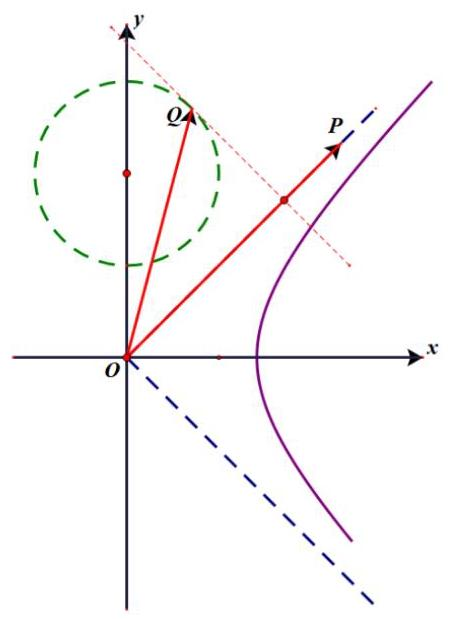
\includegraphics[max width=0.3\textwidth]{images/bo_d6dceus601uc73dvofhg_88_293_729_451_619_0.jpg}
\end{center}
\hspace*{3em} 

图 12-1

\begin{center}
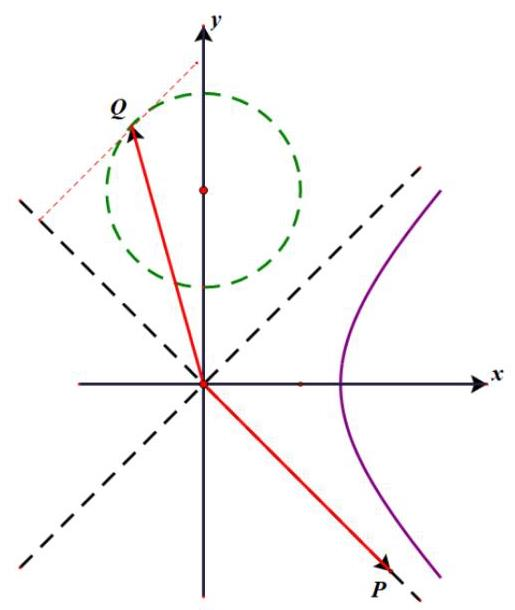
\includegraphics[max width=0.4\textwidth]{images/bo_d6dceus601uc73dvofhg_88_873_733_515_610_0.jpg}
\end{center}
\hspace*{3em} 

图 12-2

X

4.【2025.12 长宁高三一模 15】已知 \(A\left( {-2,0}\right) ,B\left( {2,0}\right)\) ,若曲线 \(\left( {\frac{x}{a} + \frac{y}{b}}\right) \left( {\frac{x}{a} - \frac{y}{b}}\right)  = 0 \; \left( {a > 0,b > 0}\right)\) 上存在点 \(P\) 满足: \(\left| {PB}\right|  = \left| {PA}\right|  + 2\) ，则 \(\frac{b}{a}\) 的取值范围( )

A. \(\left( {0,\sqrt{3}}\right)\) ; B. \(\left( {\sqrt{3}, + \infty }\right)\) ; C. \(\left( {0,\frac{\sqrt{3}}{3}}\right)\) ; D. \(\left( {\frac{\sqrt{3}}{3}, + \infty }\right)\) .

【答案】A

【解析】 \(\left| {PB}\right|  - \left| {PA}\right|  = 2\) 的点 \(P\) 的轨迹方程为 \({x}^{2} - \frac{{y}^{2}}{3} = 1\left( {x < 0}\right)\) ,渐近线为 \(y =  \pm  \sqrt{3}x\) . 若曲线 \(\left( {\frac{x}{a} - \frac{y}{b}}\right) \left( {\frac{x}{a} + \frac{y}{b}}\right)  = 0\) 上存在点 \(P\) 满足 \(\left| {PB}\right|  - \left| {PA}\right|  = 2\) , 即曲线 \(\left( {\frac{x}{a} - \frac{y}{b}}\right) \left( {\frac{x}{a} + \frac{y}{b}}\right)  = 0\) 与 \({x}^{2} - \frac{{y}^{2}}{3} = 1\left( {x < 0}\right)\) 有交点,故 \(0 < \frac{b}{a} < \sqrt{3}\) ,选 A. 3 <

5.【2025.12 宝山高三一模 15】双曲线型自然冷却通风塔的外形是由双曲线的一部分绕其虚轴所在的直线旋转一周所形成的曲面，如图所示. 已知它的下口直径为 \({20}\sqrt{10}\) 米，上口直径为 20√2 米，最小直径为 20 米，高为 80 米，则此双曲线的焦距为 ( )

\begin{center}

\includegraphics[max width=0.3\textwidth]{images/bo_d6dceus601uc73dvofhg_89_260_604_402_349_0.jpg}
\end{center}
\hspace*{3em} 

\begin{center}
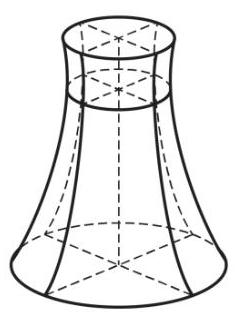
\includegraphics[max width=0.2\textwidth]{images/bo_d6dceus601uc73dvofhg_89_756_615_236_315_0.jpg}
\end{center}
\hspace*{3em} 

\begin{center}
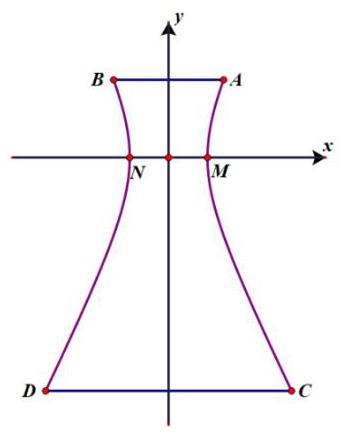
\includegraphics[max width=0.2\textwidth]{images/bo_d6dceus601uc73dvofhg_89_1035_557_340_433_0.jpg}
\end{center}
\hspace*{3em} 

A. \({10}\sqrt{3}\) . B. \({10}\sqrt{5}\) . C. \({20}\sqrt{3}\) D. \({20}\sqrt{5}\)

【答案】D

【解析】如图建系,设双曲线的标准方程为 \(\frac{{x}^{2}}{{a}^{2}} - \frac{{y}^{2}}{{b}^{2}} = 1\) ,则易得 \(a = {10}\) .

同时 \(A\left( {{10}\sqrt{2},{y}_{A}}\right) ,B\left( {{10}\sqrt{10},{y}_{B}}\right)\) ,将其分别代入双曲线方程得 \({y}_{A} = b,{y}_{B} =  - {3b}\) ,

\(\therefore {y}_{A} - {y}_{B} = {4b} = {80}\) ,解得 \(b = {20},\therefore c = \sqrt{{a}^{2} + {b}^{2}} = {10}\sqrt{5},\therefore\) 焦距为 \({2c} = {20}\sqrt{5}\) .

6.【2025.12 杨浦高三一模 15】已知双曲线 \(C : \frac{{x}^{2}}{4} - \frac{{y}^{2}}{9} = 1\) ,点 \(M\left( {4,6}\right)\) ,点 \(A,B\) 分别在双曲线 \(C\) 的左、右两支上，则向量 \(\overrightarrow{MA},\overrightarrow{MB}\) 的夹角 \(\theta\) ( ).

A. 有最大值, 但无最小值 B. 无最大值, 但有最小值

C. 既有最大值, 又有最小值 D. 既无最大值, 又无最小值

【答案】A

【解析】易得点 \(M\left( {4,6}\right)\) 在该双曲线 \(\frac{{x}^{2}}{4} - \frac{{y}^{2}}{9} = 1\) 的渐近线上,当 \(A,M,B\) 三点共线时, \(\overrightarrow{MA}\) 与 \(\overrightarrow{MB}\) 反向,即此时 \(\theta  = \pi\) 为最大值; 当 \({MB}\) 与右半支相切,同时 \({MA}\) 在第三象限无穷远处, \(\theta\) 也无线趋近于最小值,但最小值不存在,故选A.

7.【2025.12 宝山高三一模 20】已知双曲线 \(C : \frac{{x}^{2}}{{a}^{2}} - \frac{{y}^{2}}{{b}^{2}} = 1\left( {a > 0,b > 0}\right)\) 的离心率为 \(\sqrt{2}\) ,点 \(P\left( {2, - 1}\right)\) 在双曲线 \(C\) 上.

(1)求双曲线 \(C\) 的标准方程；

(2)设点 \(S\) 是双曲线 \(C\) 上的动点， \(T\) 是圆 \(E : {\left( x - 4\right) }^{2} + {y}^{2} = 1\) 上的动点，且直线 \({ST}\) 与圆 \(E\) 相切,求 \(\left| {ST}\right|\) 的最小值;

(3)如图， \(A,B\) 是双曲线 \(C\) 上两点，直线 \({PA},{PB}\) 与 \(y\) 轴分别交于点 \(M,N\) ，点 \(Q\) 在直线 \({AB}\) 上. 若 \(M,N\) 关于原点对称,且 \({PQ} \bot  {AB}\) ,证明: 存在点 \(R\) ,使得 \(\left| {QR}\right|\) 为定值.

\begin{center}
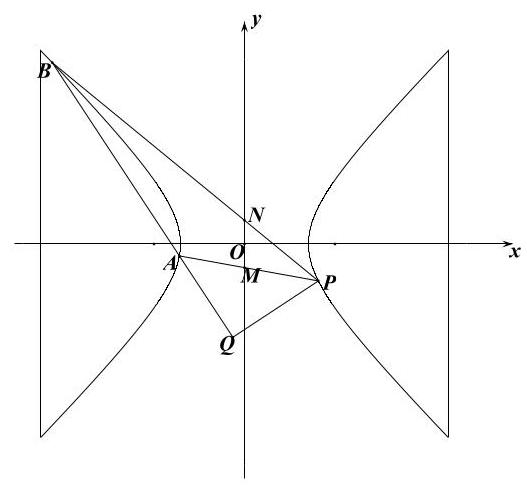
\includegraphics[max width=0.4\textwidth]{images/bo_d6dceus601uc73dvofhg_90_871_693_527_488_0.jpg}
\end{center}
\hspace*{3em} 

【答案】(1) \(\frac{{x}^{2}}{3} - \frac{{y}^{2}}{3} = 1\) (2) 2 (3)证明见解析， \(R\left( {1, - 2}\right) ,\left| {QR}\right|  = \sqrt{2}\)

【解析】(1) 由 \(e = \frac{c}{a} = \sqrt{2}\) 得 \({c}^{2} = {a}^{2} + {b}^{2} = 2{a}^{2}\) ,化简得 \({a}^{2} = {b}^{2}\)

点 \(P\left( {2, - 1}\right)\) 在双曲线 \(C\) 上,则 \(\frac{4}{{a}^{2}} - \frac{1}{{b}^{2}} = 1\) 计算得 \({a}^{2} = {b}^{2} = 3\)

所以双曲线 \(C\) 的标准方程为 \(\frac{{x}^{2}}{3} - \frac{{y}^{2}}{3} = 1\) .

(2)由题意可知 \(E\left( {4,0}\right)\) ， \(\left| {TE}\right|  = 1\) ，设 \(S\left( {{x}_{0},{y}_{0}}\right)\) ，则 \({x}_{0}{}^{2} - {y}_{0}{}^{2} = 3,\left| {x}_{0}\right|  \geq  \sqrt{3}\) ，所以

\({\left| ST\right| }^{2} = {\left| SE\right| }^{2} - 1 = {\left( {x}_{0} - 4\right) }^{2} + {y}_{0}^{2} - 1 = {\left( {x}_{0} - 4\right) }^{2} + {x}_{0}^{2} - 3 - 1\)

\(= 2{x}_{0}^{2} - 8{x}_{0} + {12} = 2{\left( {x}_{0} - 2\right) }^{2} + 4\)

当 \({x}_{0} = 2\) 时, \(\left| {ST}\right|\) 取得最小值 2 .

(3)设点 \(A\left( {{x}_{1},{y}_{1}}\right)\) 、 \(B\left( {{x}_{2},{y}_{2}}\right)\)

易知直线 \({AB}\) 的斜率存在,设直线 \({AB}\) 的方程为 \(y = {kx} + m\)

联立 \(\left\{  \begin{array}{l} {x}^{2} - {y}^{2} = 3 \\  y = {kx} + m \end{array}\right.\) 得 \(\left( {1 - {k}^{2}}\right) {x}^{2} - {2kmx} - {m}^{2} - 3 = 0\)

由韦达定理: \({x}_{1} + {x}_{2} = \frac{2km}{1 - {k}^{2}},{x}_{1}{x}_{2} = \frac{-{m}^{2} - 3}{1 - {k}^{2}}\) ,

且 \(1 - {k}^{2} \neq  0,\Delta  = 4{k}^{2}{m}^{2} - 4\left( {1 - {k}^{2}}\right) \left( {-{m}^{2} - 3}\right)  = 4\left( {{m}^{2} - 3{k}^{2} + 3}\right)  > 0\)

直线 \({PA}\) 的方程为 \(y + 1 = \frac{{y}_{1} + 1}{{x}_{1} - 2}\left( {x - 2}\right)\) ,令 \(x = 0\) 可得 \(M\left( {0, - 1 - \frac{2{y}_{1} + 2}{{x}_{1} - 2}}\right)\)

同理可得 \(N\left( {0, - 1 - \frac{2{y}_{2} + 2}{{x}_{2} - 2}}\right)\) ,因为 \(M\text{ 、 }N\) 关于原点对称,

所以 \(- 1 - \frac{2{y}_{1} + 2}{{x}_{1} - 2} +  - 1 - \frac{2{y}_{2} + 2}{{x}_{2} - 2} = 0\)

所以 \(- 1 - \frac{2\left( {k{x}_{1} + m}\right)  + 2}{{x}_{1} - 2} +  - 1 - \frac{2\left( {k{x}_{2} + m}\right)  + 2}{{x}_{2} - 2} = 0\)

整理得 \(\left( {{2k} + 1}\right) {x}_{1}{x}_{2} + \left( {m - {2k} - 1}\right) \left( {{x}_{1} + {x}_{2}}\right)  - {4m} = 0\)

代入韦达定理得 \(\left( {{2k} + 1}\right) \frac{{m}^{2} + 3}{{k}^{2} - 1} + \left( {m - {2k} - 1}\right) \frac{-{2km}}{{k}^{2} - 1} = {4m}\)

化简得 \({m}^{2} + \left( {{2k} + 4}\right) m + 3\left( {{2k} + 1}\right)  = 0\) ,即 \(\left( {m + 3}\right) \left( {m + {2k} + 1}\right)  = 0\)

当 \(m + {2k} + 1 = 0\) 时,直线 \({AB}\) 的方程为 \(y = {kx} - {2k} - 1 = k\left( {x - 2}\right)  - 1\) 此时直线过点 \(P\left( {2, - 1}\right)\) ,不合题意,舍;

当 \(m =  - 3\) 时,直线 \({AB}\) 的方程为 \(y = {kx} - 3\) ,此时直线过定点 \(D\left( {0, - 3}\right)\)

则 \(\left| {PD}\right|  = \sqrt{{2}^{2} + {2}^{2}} = 2\sqrt{2}\) 为定值，

又 \({PQ} \bot  {AB}\) ,所以当 \(R\) 为 \({PD}\) 中点时, \(\left| {QR}\right|  = \frac{1}{2}\left| {PD}\right|  = \sqrt{2}\) 也为定值,此时 \(R\left( {1, - 2}\right)\) .

8.【2025.12 黄浦高三一模 20】已知双曲线 \(\Gamma\) 的中心位于坐标原点 \(O\) ,焦点 \({F}_{2},{F}_{1}\) 分别在 \(x\) 轴的正、负半轴上, \(\left| {{F}_{1}{F}_{2}}\right|  = 2\sqrt{2}\) ,直线 \(y =  - x\) 是 \(\Gamma\) 的一条渐近线,直线 \({l}_{1} : y = \sqrt{2}x + t\left( {t < 0}\right)\) 与 \(\Gamma\) 有且只有一个公共点 \(P\) .

(1)求 \(\Gamma\) 的方程；

(2)若点 \(Q\) 在 \(y\) 轴上，且 \(\angle {F}_{1}{QP}\) 为直角，求点 \(Q\) 的坐标；

(3)设动直线 \({l}_{2}\) 平行于 \({OP}\) ，与 \(\Gamma\) 交于点 \(A\) ， \(B\) ，与 \({l}_{1}\) 交于点 \(K\) ，是否存在常数 \(\lambda\) ，使得 \(\left| {KA}\right|  \cdot  \left| {KB}\right|  = \lambda {\left| KP\right| }^{2}\) 总成立? 若存在,请求出 \(\lambda\) 的值; 若不存在,请说明理由.

\begin{center}
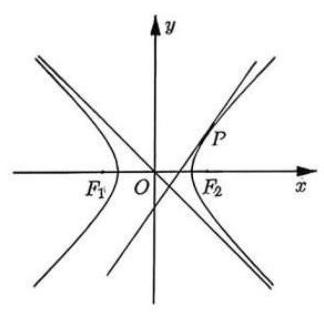
\includegraphics[max width=0.2\textwidth]{images/bo_d6dceus601uc73dvofhg_92_251_217_324_313_0.jpg}
\end{center}
\hspace*{3em} 

\begin{center}
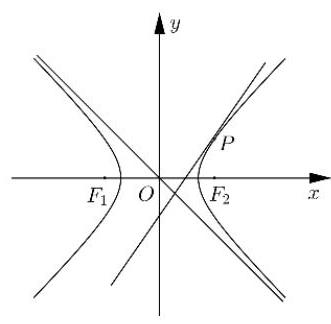
\includegraphics[max width=0.2\textwidth]{images/bo_d6dceus601uc73dvofhg_92_651_208_331_324_0.jpg}
\end{center}
\hspace*{3em} 

\begin{center}
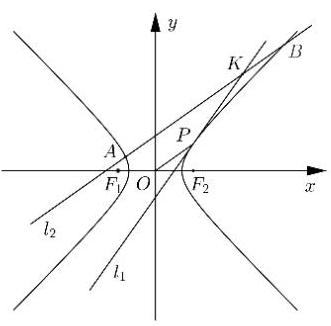
\includegraphics[max width=0.2\textwidth]{images/bo_d6dceus601uc73dvofhg_92_986_206_331_326_0.jpg}
\end{center}
\hspace*{3em} 

【答案】(1) \({x}^{2} - {y}^{2} = 1\) (2) \(\left( {0,2}\right)\) 或 \(\left( {0, - 1}\right)\) . (3)存在 \(\lambda  = 1\) 符合题意

【解析】(1) 设 \(\Gamma\) 的方程为 \(\frac{{x}^{2}}{{a}^{2}} - \frac{{y}^{2}}{{b}^{2}} = 1\left( {a > 0,b > 0}\right) ,\Gamma\) 的焦距为 \({2c}\) ,则 \({2c} = 2\sqrt{2}\) ,即 \(c = \sqrt{2}\) , 由 \(y = x\) 是 \(\Gamma\) 的一条渐近线,可知 \(\frac{b}{a} = 1\) ,即 \(a = b\) ,故 \(c = \sqrt{{a}^{2} + {b}^{2}} = \sqrt{2}a\) ,可得 \(a = 1,b = 1\) , 所以 \(\Gamma\) 的方程为 \({x}^{2} - {y}^{2} = 1\) . .4 分

(2)由 \(\left\{  \begin{matrix} y = \sqrt{2}x + t, \\  {x}^{2} - {y}^{2} = 1, \end{matrix}\right.\) 消去 \(y\) 得 \({x}^{2} + 2\sqrt{2}{tx} + {t}^{2} + 1 = 0\) ，由 \(\Delta  =\)

\(4{t}^{2} - 4 = 0\) 且 \(t < 0\) ,可得 \(t =  - 1\) ,此时点 \(P\) 的坐标为 \(\left( {\sqrt{2},1}\right) .\ldots 7\) 分

设 \(Q\left( {0,n}\right)\) ,由 \(\angle {F}_{1}{QP}\) 为直角 \(\Leftrightarrow\) 向量 \(\overrightarrow{Q{F}_{1}} \bot  \overrightarrow{QP} \Leftrightarrow  \overrightarrow{Q{F}_{1}} \cdot  \overrightarrow{QP} = 0\) ,

可得 \(\left( {-\sqrt{2}, - n}\right)  \cdot  \left( {\sqrt{2},1 - n}\right)  = 0\) ,即 \({n}^{2} - n - 2 = 0\) ,解得 \(n = 2\) 或 \(n =  - 1\) ,

故点 \(Q\) 的坐标为 \(\left( {0,2}\right)\) 或 \(\left( {0, - 1}\right)\) . .10 分

(3) \(\because {OP}\) 的斜率为 \(\frac{\sqrt{2}}{2}\) ，故可设 \({l}_{2}\) 的方程为 \(y = \frac{\sqrt{2}}{2}x + m\left( {m \neq  0}\right)\) . .11 分

由 \(K\) 在直线 \({l}_{1}\) 上,故可设 \(K\left( {{x}_{0},\sqrt{2}{x}_{0} - 1}\right)\) ,代入 \(y = \frac{\sqrt{2}}{2}x + m\) ,可得 \(m = \frac{\sqrt{2}}{2}\left( {{x}_{0} - \sqrt{2}}\right)\) ,

故 \({\left| KP\right| }^{2} = \left\lbrack  {1 + {\left( -\sqrt{2}\right) }^{2}}\right\rbrack  {\left( {x}_{0} - \sqrt{2}\right) }^{2} = 6{m}^{2}\) , .13 分

将 \({l}_{2}\) 的方程代入 \(\Gamma\) 的方程,可得 \({x}^{2} - 2\sqrt{2}{mx} - 2\left( {{m}^{2} + 1}\right)  = 0\) ,

设点 \(A,B\) 的横坐标分别为 \({x}_{1},{x}_{2}\) ,则 \(\left\{  \begin{matrix} {x}_{1} + {x}_{2} = 2\sqrt{2}m, \\  {x}_{1}{x}_{2} =  - 2\left( {{m}^{2} + 1}\right) , \end{matrix}\right.\)

故 \(\left| {KA}\right|  \cdot  \left| {KB}\right|  = \sqrt{1 + \frac{1}{2}}\left| {{x}_{1} - {x}_{0}}\right|  \cdot  \sqrt{1 + \frac{1}{2}}\left| {{x}_{2} - {x}_{0}}\right|\)

\(=  - \frac{3}{2}\left( {{x}_{1} - {x}_{0}}\right) \left( {{x}_{2} - {x}_{0}}\right)  =  - \frac{3}{2}\left\lbrack  {{x}_{1}{x}_{2} - {x}_{0}\left( {{x}_{1} + {x}_{2}}\right)  + {x}_{0}^{2}}\right\rbrack\)

\(=  - \frac{3}{2}\left\lbrack  {-2\left( {1 + {m}^{2}}\right)  - \sqrt{2}\left( {1 + m}\right) \left( {2\sqrt{2}m}\right)  + 2{\left( 1 + m\right) }^{2}}\right\rbrack   = 6{m}^{2},\) .17 分

故当 \(\lambda  = 1\) 时, \(\left| {KA}\right|  \cdot  \left| {KB}\right|  = \lambda {\left| KP\right| }^{2}\) ,

所以存在常数 \(\lambda\) ,使得 \(\left| {KA}\right|  \cdot  \left| {KB}\right|  = \lambda {\left| KP\right| }^{2}\) 总成立. .18 分Ⓡ

9.【2025.12 静安高三一模 20】在平面直角坐标系 \({xOy}\) 中,已知双曲线 \(\Gamma  : \frac{{x}^{2}}{{a}^{2}} - \frac{{y}^{2}}{{b}^{2}} = 1\left( {a > 0,b > 0}\right)\) 的焦距为 4,点 \(\left( {\sqrt{6},1}\right)\) 在 \(\Gamma\) 上.

(1)求双曲线 \(\Gamma\) 的方程；

(2)设直线 \(l\) 的斜率为 \(\frac{1}{2}\) ， \(l\) 交双曲线 \(\Gamma\) 于 \(P\) 、 \(Q\) 两点，且与圆 \({x}^{2} + {y}^{2} = 4\) 相切，切点位于 \(x\) 轴上方部分,求 \(\overrightarrow{OP} \cdot  \overrightarrow{OQ}\) 的值;

(3)如图，设过双曲线 \(\Gamma\) 的左焦点 \({F}_{1}\) 的直线 \({AB}\) 交 \(\Gamma\) 的左支于点 \(A\) 、 \(B\) ，过 \(\Gamma\) 的右焦点 \({F}_{2}\) 的直线 \({CD}\) 交 \(\Gamma\) 的右支于点 \(C\) 、 \(D\) ，若直线 \({CD}//{AB}\) ，且四边形 \({ABCD}\) 的面积为 \(4\sqrt{6}\) ，求直线 \({AB}\) 的方程.

【答案】(1) \(\frac{{x}^{2}}{3} - {y}^{2} = 1\) (3) \(x - y + 2 = 0\) 或 \(x + y + 2 = 0\) .

【解析】(1) 由双曲线 \(\Gamma  : \frac{{x}^{2}}{{a}^{2}} - \frac{{y}^{2}}{{b}^{2}} = 1\left( {a > 0,b > 0}\right)\) 的焦距为4,点 \(\left( {6,1}\right)\) 在 \(\Gamma\) 上, 可得 \({2c} = 4\) ,所以 \(c = 2\) ,且 \(\frac{6}{{a}^{2}} - \frac{1}{{b}^{2}} = 1\) ,又因为 \({c}^{2} = {a}^{2} + {b}^{2}\) ,即 \({a}^{2} + {b}^{2} = 4\) , 联立方程组 \(\left\{  \begin{array}{l} {a}^{2} + {b}^{2} = 4 \\  \frac{6}{{a}^{2}} - \frac{1}{{b}^{2}} = 1 \end{array}\right.\) ,解得 \({a}^{2} = 3,{b}^{2} = 1\) ,所以 \(\Gamma\) 的方程为 \(\frac{{x}^{2}}{3} - {y}^{2} = 1\) .

(2)设直线 \(l\) 方程为 \(y = \frac{1}{2}x + m\) ，代入圆的方程整理得 \(\frac{5}{4}{x}^{2} + {mx} + {m}^{2} - 4 = 0\) ，

直线与圆相切，所以判别式 \(\Delta  = {m}^{2} - 5{m}^{2} + {20} = 0\) ，所以 \({m}^{2} = 5\) ，

切点位于 \(x\) 轴上方,故 \(m = \sqrt{5}\) .

将直线 \(y = \frac{1}{2}x + \sqrt{5}\) 代入双曲线 \(\Gamma\) 方程,整理得 \(\frac{1}{12}{x}^{2} - \sqrt{5}x - 6 = 0\) ,解得 \(x = 6\left( {\sqrt{5} \pm  \sqrt{7}}\right)\) ,

\(P\text{ 、 }Q\) 两点的坐标分别为 \(\left( {6\sqrt{5} - 6\sqrt{7},4\sqrt{5} - 3\sqrt{7}}\right) \text{ 、 }\left( {6\sqrt{5} + 6\sqrt{7},4\sqrt{5} + 3\sqrt{7}}\right)\)

从而 \(\overrightarrow{OP} \cdot  \overrightarrow{OQ} = {180} - {252} + {80} - {63} =  - {55}\) ;

另解: 由题意设直线 \(l\) 方程为 \(y = \frac{1}{2}x + m\left( {m > 0}\right)\) ,该直线与圆 \({x}^{2} + {y}^{2} = 4\) 相切,

则圆心到直线 \(l\) 的距离 \(d = \frac{\left| 2m\right| }{\sqrt{5}} = 2\) ,解得 \(m = \sqrt{5}\) .

联立 \(\left\{  \begin{array}{l} y = \frac{1}{2}x + \sqrt{5} \\  \frac{{x}^{2}}{3} - {y}^{2} = 1 \end{array}\right.\) ,得 \({x}^{2} - {12}\sqrt{5}x - {72} = 0\)

设 \(P\left( {{x}_{1},{y}_{1}}\right) ,Q\left( {{x}_{2},{y}_{2}}\right)\) ,则 \({x}_{1} + {x}_{2} = {12}\sqrt{5},{x}_{1} \cdot  {x}_{2} =  - {72}\)

\(\overrightarrow{OP} \cdot  \overrightarrow{OQ} = {x}_{1}{x}_{2} + {y}_{1}{y}_{2} = {x}_{1}{x}_{2} + \left( {\frac{1}{2}{x}_{1} + \sqrt{5}}\right) \left( {\frac{1}{2}{x}_{2} + \sqrt{5}}\right)  = \frac{5}{4}{x}_{1}{x}_{2} + \frac{\sqrt{5}}{2}\left( {{x}_{1} + {x}_{2}}\right)  + 5\)

\(= \frac{5}{4} \times  \left( {-{72}}\right)  + \frac{\sqrt{5}}{2} \times  {12}\sqrt{5} + 5 =  - {55}\)

(3)由题意直线 \({AB}\) 与 \({CD}\) 平行，由双曲线的对称性，易知 \({AB} = {CD}\) ，四边形 \({ABCD}\) 为平行四边形.

此时四边形 \(\mathrm{{ABCD}}\) 的面积为 \(\frac{8\sqrt{3}}{3}\) ,不合题意,舍去;

设直线 \({AB}\) 方程为 \(y = k\left( {x + 2}\right)\) ,则直线 \({CD}\) 方程为 \(y = k\left( {x - 2}\right)\) ,

直线 \({AB}\) 和 \({CD}\) 的距离就是点 \({F}_{2}\) 到直线 \({AB}\) 的距离 \(d = \frac{\left| 4k\right| }{\sqrt{1 + {k}^{2}}}\) ,设 \(A\left( {{x}_{1},{y}_{1}}\right) ,B\left( {{x}_{2},{y}_{2}}\right)\) ,

联立方程组 \(\left\{  \begin{array}{l} \frac{{x}^{2}}{3} - {y}^{2} = 1 \\  y = k\left( {x + 2}\right)  \end{array}\right.\) ,整理得 \(\left( {1 - 3{k}^{2}}\right) {x}^{2} - {12}{k}^{2}x - {12}{k}^{2} - 3 = 0\) ,

则 \(\Delta  = {12}\left( {{k}^{2} + 1}\right)  > 0\) ,且 \({x}_{1} + {x}_{2} = \frac{{12}{k}^{2}}{1 - 3{k}^{2}},{x}_{1}{x}_{2} = \frac{-{12}{k}^{2} - 3}{1 - 3{k}^{2}}\) ,

又由双曲线的渐近线的方程为 \(y =  \pm  \frac{\sqrt{3}}{3}x\) ,要使得过 \(\Gamma\) 的左焦点 \({F}_{1}\) 的直线 \({AB}\) 交 \(\Gamma\) 的左支于点 \(A,B\) ,可得 \({k}^{2} > \frac{1}{3},\left( {{x}_{1}{x}_{2} > 0}\right)\)

则 \(\left| {AB}\right|  = \sqrt{1 + {k}^{2}}\left| {{x}_{1} - {x}_{2}}\right|  = \sqrt{1 + {k}^{2}}\sqrt{{\left( {x}_{1} + {x}_{2}\right) }^{2} - 4{x}_{1}{x}_{2}}\)

\(= \sqrt{1 + {k}^{2}}\sqrt{{\left( \frac{{12}{k}^{2}}{1 - 3{k}^{2}}\right) }^{2} + \frac{{48}{k}^{2} + 2}{1 - 3{k}^{2}}} = \frac{2\sqrt{3}\left( {1 + {k}^{2}}\right) }{3{k}^{2} - 1}\) ,

所以 \({S}_{ABCD} = \left| {AB}\right|  \times  d = \frac{2\sqrt{3}\left( {1 + {k}^{2}}\right) }{3{k}^{2} - 1} \times  \frac{\left| 4k\right| }{\sqrt{1 + {k}^{2}}} = \frac{8\sqrt{3}\left| k\right| \sqrt{1 + {k}^{2}}}{3{k}^{2} - 1} = 4\sqrt{6}\) ,

化简可得 \(7{k}^{4} - 8{k}^{2} + 1 = 0\) ,解得 \({k}^{2} = \frac{1}{7}\) ,或 \({k}^{2} = 1\) ,因为 \({k}^{2} > \frac{1}{3}\) ,所以 \({k}^{2} = 1\) ,

故直线 \({AB}\) 的方程为 \(x - y + 2 = 0\) 或 \(x + y + 2 = 0\) .

另解: 设直线 \({AB}\) 方程为 \(x = {ky} - 2\) ,代入双曲线方程得 \(\frac{{\left( ky - 2\right) }^{2}}{3} - {y}^{2} = 1\) ,

整理得 \(\left( {{k}^{2} - 3}\right) {y}^{2} - {4ky} + 1 = 0\) ,(因为双曲线的渐近线斜率为 \(\frac{\sqrt{3}}{3}\) ,直线 \(\mathrm{{AB}}\) 与双曲线左支交于两点,所以 \({k}^{2} \neq  3),{y}_{1} + {y}_{2} = \frac{4k}{{k}^{2} - 3},{y}_{1}{y}_{2} = \frac{1}{{k}^{2} - 3}\) ,

所以 \(\left| {AB}\right|  = \sqrt{1 + {k}^{2}}\sqrt{{\left( {y}_{1} - {y}_{2}\right) }^{2}} = \sqrt{1 + {k}^{2}}\sqrt{{\left( {y}_{1} + {y}_{2}\right) }^{2} - 4{y}_{1}{y}_{2}}\) ,

点 \({F}_{2}\) 到直线 \({AB}\) 的距离 \(d = \frac{4}{\sqrt{1 + {k}^{2}}}\) ,

\({S}_{ABCD} = \left| {AB}\right|  \times  d = \frac{\sqrt{1 + {k}^{2}}}{\left| {k}^{2} - 3\right| } \times  \sqrt{{12}{k}^{2} + {12}} \times  \frac{4}{\sqrt{1 + {k}^{2}}} = \frac{8\sqrt{3}\sqrt{1 + {k}^{2}}}{\left| {k}^{2} - 3\right| } = 4\sqrt{6},\)

化简可得 \({k}^{4} - 8{k}^{2} + 7 = 0\) ,解得 \({k}^{2} = 7\) ,或 \({k}^{2} = 1\) ,

因为当 \({k}^{2} = 7\) 时,直线 \(\mathrm{{AB}}\) 斜率平方 \(\frac{1}{{k}^{2}} < \frac{1}{7}\) ,此时 \(\mathrm{{AB}}\) 与双曲线左支只能交于一点,舍去, 所以 \({k}^{2} = 1\) ,故直线 \({AB}\) 的方程为 \(x - y + 2 = 0\) ,或 \(x + y + 2 = 0\) . \(>\)

10.【2025.12 闵行高三一模 20】已知双曲线 \(\Gamma  : {x}^{2} - {y}^{2} = 1\) ，直线 \(l\) 过点 \(M\left( {m,0}\right) ,m \in  \mathbf{R}\) ，且与 \(\Gamma\) 的右支交于 \(P\text{ 、 }Q\) 两点,与 \(\Gamma\) 的两条渐近线分别交于 \(A\text{ 、 }B\) 两点,其中 \(A\text{ 、 }P\) 在第一象限, \(B\text{ 、 }Q\) 在第四象限.

(1)求 \(\Gamma\) 的两条渐近线的夹角；

(2)若 \(M\) 为 \(\Gamma\) 的右焦点，求 \(\bigtriangleup  {OAB}\) 的面积的最小值；

(3)若 \(\left| {AP}\right|  = \left| {PQ}\right|  = \left| {QB}\right|\) ，求 \(m\) 的取值范围.

【答案】(1) \(\frac{\pi }{2}\) (2) 2

(3) \(m \in  \left( {1,\frac{3\sqrt{2}}{4}}\right\rbrack\)

【解析】(1) 由题意得双曲线的两条渐近线为 \(y =  \pm  x\) ,夹角为 \(\frac{\pi }{2}\) .

(2)由题意，右焦点为 \(M\left( {\sqrt{2},0}\right)\) ，

设 \(l : x = {ty} + \sqrt{2}\) , \(A\left( {{x}_{A},{x}_{A}}\right) ,B\left( {{x}_{B},{x}_{B}}\right)\) ,则 \(\left\{  {\begin{array}{l} x = {ty} + \sqrt{2} \\  y = x \end{array} \Rightarrow  x = {tx} + \sqrt{2}}\right.\) ,

\(\left( {1 - t}\right) x = \sqrt{2}\) ,显然 \(t \neq  1,{x}_{A} = \frac{\sqrt{2}}{1 - t}\) ,因 \(A\) 在第一象限,所以 \({x}_{A} = \frac{\sqrt{2}}{1 - t} > 0\) ,所以 \(t < 1\) ;

同理 \({x}_{B} = \frac{\sqrt{2}}{1 + t} > 0,t >  - 1\) . 所以 \(- 1 < t < 1\) .

故 \({S}_{\bigtriangleup {OAB}} = \frac{1}{2}\left| {OA}\right|  \cdot  \left| {OB}\right|  = \frac{1}{2}\left| {\sqrt{2}{x}_{A}}\right|  \cdot  \left| {\sqrt{2}{x}_{B}}\right|  = \left| {{x}_{A}{x}_{B}}\right|  = \frac{2}{1 - {t}^{2}} \geq  2\) ,

当且仅当 \(t = 0\) 时取等号,此时 \(l : x = \sqrt{2}\) ,存在四点 \(A\text{ 、 }B\text{ 、 }P\text{ 、 }Q\) 满足题意.

所以 \(\bigtriangleup {OAB}\) 的面积的最小值为 2 .

(3)设 \(l\) 的方程为 \(x = {ty} + m\) ,联立 \(\left\{  \begin{array}{l} x = {ty} + m \\  {x}^{2} - {y}^{2} = 0 \end{array}\right.\) ，得 \(\left( {{t}^{2} - 1}\right) {y}^{2} + {2tm}y + {m}^{2} = 0\) ，显然 \(t \neq   \pm  1\) ， 设 \(A\left( {{x}_{1},{y}_{1}}\right) \text{ 、 }B\left( {{x}_{2},{y}_{2}}\right)\) ,则 \({y}_{1} + {y}_{2} =  - \frac{2tm}{{t}^{2} - 1},{y}_{1}{y}_{2} = \frac{{m}^{2}}{{t}^{2} - 1}\) ,

由题意 \({y}_{1} > 0,{y}_{2} < 0\) ,所以 \({y}_{1}{y}_{2} = \frac{{m}^{2}}{{t}^{2} - 1} < 0\) ,所以 \(- 1 < t < 1,m \neq  0\)

联立 \(\left\{  \begin{array}{l} x = {ty} + m \\  {x}^{2} - {y}^{2} = 1 \end{array}\right.\) ,得 \(\left( {{t}^{2} - 1}\right) {y}^{2} + {2tmy} + {m}^{2} - 1 = 0\) ,

设 \(P\left( {{x}_{3},{y}_{3}}\right) \text{ 、 }Q\left( {{x}_{4},{y}_{4}}\right)\) ,则 \({y}_{3} + {y}_{4} =  - \frac{2tm}{{t}^{2} - 1},{y}_{3}{y}_{4} = \frac{{m}^{2} - 1}{{t}^{2} - 1}\) ,

由 \({y}_{3}{y}_{4} = \frac{{m}^{2} - 1}{{t}^{2} - 1} < 0\) ,得 \({m}^{2} - 1 > 0\) ,

又 \(A\text{ 、 }B\text{ 、 }M\) 三点共线,且 \(A\text{ 、 }B\) 在第一、三象限, \(M\) 在 \(x\) 轴上,

故 \(m > 0\) ,所以 \(m > 1\) .

由 \({y}_{1} + {y}_{2} =  - \frac{2tm}{{t}^{2} - 1} = {y}_{3} + {y}_{4}\) ,得线段 \({AB}\) 与 \({PQ}\) 的中点重合,所以 \(\left| {AP}\right|  = \left| {QB}\right|\) .

由 \(\left| {AP}\right|  = \left| {PQ}\right|  = \left| {QB}\right|\) ,得 \(\left| {AB}\right|  = 3\left| {PQ}\right|\) ,因此 \(\left| {{y}_{1} - {y}_{2}}\right|  = 3\left| {{y}_{3} - {y}_{4}}\right|\) ,

所以 \({\left( {y}_{1} + {y}_{2}\right) }^{2} - 4{y}_{1}{y}_{2} = 9\left\lbrack  {{\left( {y}_{3} + {y}_{4}\right) }^{2} - 4{y}_{3}{y}_{4}}\right\rbrack\) ,

由此可得, \({\left( -\frac{2tm}{{t}^{2} - 1}\right) }^{2} - 4\frac{{m}^{2}}{{t}^{2} - 1} = 9\left\lbrack  {{\left( -\frac{2tm}{{t}^{2} - 1}\right) }^{2} - 4\frac{{m}^{2} - 1}{{t}^{2} - 1}}\right\rbrack\) ,整理得 \(\frac{8{t}^{2}}{{t}^{2} - 1} = \frac{8{m}^{2} - 9}{{m}^{2}}\) ,

因为 \({t}^{2} \in  \lbrack 0,1)\) ,所以 \(\frac{8{m}^{2} - 9}{{m}^{2}} \leq  0\) ,又由 \(m > 1\) ,所以 \(m\) 的取值范围为 \(\left( {1,\frac{3\sqrt{2}}{4}}\right\rbrack\) . \(\ll\)

\section*{7.4 抛物线}

\section*{【知识梳理】}

\section*{1.抛物线的定义}

平面上到一个定点 \(F\) 和到一条定直线 \(l\) ( \(F\) 不在 \(l\) 上) 距离相等的点的轨迹叫做抛物线. 点 \(F\) 叫做抛物线的焦点, 定直线/叫做抛物线的准线.

\section*{2.抛物线的标准方程与几何性质}

\begin{center}
\adjustbox{max width=\textwidth}{
\begin{tabular}{|c|c|c|c|c|}
\hline
\multirow{2}{*}{标准方程} & \({y}^{2} = {2px}\left( {p > 0}\right)\) & \({y}^{2} =  - {2px}\left( {p > 0}\right)\) & \({x}^{2} = {2py}\left( {p > 0}\right)\) & \({x}^{2} =  - {2py}\left( {p > 0}\right)\) \\
\cline{2-5}
 & \multicolumn{4}{|c|}{\(p\) 的几何意义: 焦点 \(F\) 到准线 \(l\) 的距离} \\
\cline{1-5}
图形 & 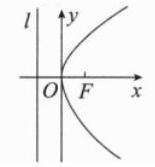
\includegraphics[max width=0.2\textwidth]{images/bo_d6dceus601uc73dvofhg_97_485_767_155_167_0.jpg} & 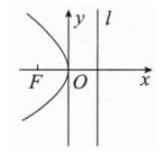
\includegraphics[max width=0.2\textwidth]{images/bo_d6dceus601uc73dvofhg_97_720_770_164_154_0.jpg} & 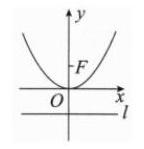
\includegraphics[max width=0.2\textwidth]{images/bo_d6dceus601uc73dvofhg_97_970_774_144_149_0.jpg} & 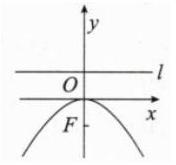
\includegraphics[max width=0.2\textwidth]{images/bo_d6dceus601uc73dvofhg_97_1194_766_176_165_0.jpg} \\
\cline{1-5}
顶点 & \multicolumn{4}{|c|}{\(O\left( {0,0}\right)\)} \\
\cline{1-5}
对称轴 & \multicolumn{2}{|c|}{\(x\) 轴} & \multicolumn{2}{|c|}{\(y\) 轴} \\
\cline{1-5}
焦点 & \(F\left( {\frac{p}{2},0}\right)\) & \(F\left( {-\frac{p}{2},0}\right)\) & \(F\left( {0,\frac{p}{2}}\right)\) & \(F\left( {0, - \frac{p}{2}}\right)\) \\
\cline{1-5}
离心率 & \multicolumn{4}{|c|}{\(e = 1\)} \\
\cline{1-5}
准线方程 & \(x =  - \frac{p}{2}\) & \(x = \frac{p}{2}\) & \(y =  - \frac{p}{2}\) & \(y = \frac{p}{2}\) \\
\cline{1-5}
范围 & \(x \geq  0,\;y \in  \mathbf{R}\) & \(x \leq  0,\;y \in  \mathbf{R}\) & \(y \geq  0,\;x \in  \mathbf{R}\) & \(y \leq  0,\;x \in  \mathbf{R}\) \\
\cline{1-5}
开口方向 & 向右 & 向左 & 向上 & 向下 \\
\cline{1-5}
焦半径(其中 \(P\left( {{x}_{0},{y}_{0}}\right)\) ) & \(\left| {PF}\right|  = {x}_{0} + \frac{p}{2}\) & \(\left| {PF}\right|  =  - {x}_{0} + \frac{p}{2}\) & \(\left| {PF}\right|  = {y}_{0} + \frac{p}{2}\) & \(\left| {PF}\right|  =  - {y}_{0} + \frac{p}{2}\) \\
\cline{1-5}
\hline
\end{tabular}
}
\end{center}

1.【2025.12 宝山高三一模 2】焦点为 \(\left( {1,0}\right)\) 的抛物线的标准方程为\_\_\_\_\_.

【答案】 \({y}^{2} = {4x}\) .

2.【2025.12 松江高三一模 2】抛物线 \({y}^{2} = {8x}\) 的焦点到其准线的距离为\_\_\_\_\_.

【答案】 4

【解析】焦点为 \(\left( {2,0}\right)\) ,准线为 \(x =  - 2\) ,所以距离为4.

3.【2025.12 崇明高三一模 5】抛物线 \({y}^{2} = {4x}\) 的准线方程是\_\_\_\_\_.

【答案】 \(x =  - 1 >\)

4.【2025.12 静安高三一模 9】抛物线具有如下的光学性质:所有平行于抛物线对称轴的入射光线经抛物线反射后都过这条抛物线的焦点. 设抛物线的方程为 \({y}^{2} = {12x}\) ，一束光线从平行于其对称轴方向射向抛物线,光线所在直线交抛物线 \({y}^{2} = {12x}\) 于一点,这点的纵坐标为 12. 则这束光线经过抛物线反射后所在直线的一个法向量为\_\_\_\_\_.

【答案】 \(\left( {4, - 3}\right)\)

【解析】依题意可得: 光线与抛物线交点坐标为 \(P\left( {{12},{12}}\right)\) ,同时,其焦点为 \(F\left( {3,0}\right)\) , \(\therefore\) 直线 \({PF}\) 的方程为 \(y = \frac{4}{3}\left( {x - 3}\right)\) ,即 \({4x} - {3y} - {12} = 0,\therefore\) 一个法向量为 \(\left( {4, - 3}\right)\) .

5.【2025.12 闵行高三一模 13】抛物线 \({y}^{2} = x\) 的准线方程为( ).

A. \(x = \frac{1}{4}\) B. \(x =  - \frac{1}{4}\) C. \(y = \frac{1}{4}\) D. \(y =  - \frac{1}{4}\)

【答案】B

【解析】抛物线 \({y}^{2} = x\) 的准线方程为 \(x =  - \frac{1}{4}\) ,故选: B.

6.【2025.12 普陀高三一模 15】设点 \(M\) 是抛物线 \({x}^{2} = 8\sqrt{5}y\) 的焦点,点 \(F\) 是双曲线 \(\Gamma  : {x}^{2} - \frac{{y}^{2}}{4} = 1\) 的左焦点,点 \(Q\) 是 \(\Gamma\) 上在第一象限内的一动点,则下列结论中正确的是 ( ).

A. \(\left| {QF}\right|  - \left| {QM}\right|\) 的最大值是 5 B. \(\left| {QF}\right|  + \left| {QM}\right|\) 的最小值是 5

C. \(\left| {QF}\right|  - \left| {QM}\right|\) 的最大值是 7 D. \(\left| {QF}\right|  + \left| {QM}\right|\) 的最小值是 7

【答案】D

【解析】依题意可得: \(M\left( {0,2\sqrt{5}}\right) ,F\left( {-\sqrt{5},0}\right)\) ,设右焦点为 \({F}_{2}\left( {\sqrt{5},0}\right)\) .

同时,渐近线为 \(y =  \pm  {2x}\) ,所以直线 \({MF}\) 与其中一条渐近线 \(y = {2x}\) 平行.

所以当 \(Q\) 在 \(\Gamma\) 上的第一象限内时, \(\left| {QF}\right|  - \left| {QM}\right|  < \left| {QF}\right|\) ,但不能取等,

故 \(\left| {QF}\right|  - \left| {QM}\right|\) 并无最大值. 此时 \(\left| {QF}\right|  + \left| {QM}\right|  = 2 + \left| {Q{F}_{2}}\right|  + \left| {QM}\right|  \geq  2 + \left| {M{F}_{2}}\right|  = 7\) ,

当且仅当 \(Q,M,{F}_{2}\) 三点共线时,等号成立. 故 \(\left| {QF}\right|  + \left| {QM}\right|\) 的最小值为 7,选 D.S.

7.【2025.12 长宁高三一模 20】已知抛物线 \(\Gamma  : {y}^{2} = {4x}\) 的焦点为 \(\mathrm{F}\) ，经过点 \(\mathrm{F}\) 的直线 \(l\) 与抛物线 \(\Gamma\) 交于 \(\mathrm{A}\text{ 、 }\mathrm{\;B}\) 两点.

(1)设 \(\left| {AF}\right|  = 5\) ，求点 \(\mathrm{A}\) 的横坐标；

(2)设 \(\mathrm{O}\) 为坐标原点，线段 \(\mathrm{{AB}}\) 中点的纵坐标为 \(\frac{3}{2}\) ，求 \(\bigtriangleup  \mathrm{{OAB}}\) 的面积；

(3)设线段 \(\mathrm{{AB}}\) 的垂直平分线与抛物线 \(\Gamma\) 交于点 \(\mathrm{M}\) 、 \(\mathrm{N}\) ，若以线段 \(\mathrm{{MN}}\) 为直径的圆经过点 \(\mathrm{A}\text{ 、 }\mathrm{\;B}\) ,求直线 \(l\) 的方程.

【答案】(1)4 (2) \(S = \frac{1}{2}\left| {OF}\right| \left| {{y}_{1} - {y}_{2}}\right|  = \frac{5}{2}\) (3) \(y = x - 1\) 或 \(y =  - x + 1\) .

【解析】(1) 设 \(A\left( {{x}_{1},{y}_{1}}\right) ,F\left( {1,0}\right)\) ,

因为 \(\left| {AF}\right|  = 5\) ,所以 \({x}_{1} + 1 = 5,{x}_{1} = 4\) ,点 \(\mathrm{A}\) 的横坐标为 4

(2)设 \(A\left( {{x}_{1},{y}_{1}}\right) ,B\left( {{x}_{2},{y}_{2}}\right)\) ，因为 \(\mathrm{{AB}}\) 中点纵坐标为 \(\frac{3}{2}\) ，所以 \({y}_{1} + {y}_{2} = 3\) ，

直线 \(l\) 的斜率 \(k = \frac{{y}_{1} - {y}_{2}}{{x}_{1} - {x}_{2}} = \frac{4}{{y}_{1} + {y}_{2}} = \frac{4}{3}\) ，直线 \(l\) 的方程为 \(y = \frac{4}{3}\left( {x - 1}\right)\) ，

将直线方程代入抛物线方程得 \({y}^{2} - {3y} - 4 = 0\) ，

\({y}_{1} =  - 1,\;{y}_{2} = 4,\;\bigtriangleup \mathrm{{OAB}}\) 的面积 \(S = \frac{1}{2}\left| {OF}\right| \left| {{y}_{1} - {y}_{2}}\right|  = \frac{5}{2}\) .

(3)设 \(A\left( {{x}_{1},{y}_{1}}\right) ,B\left( {{x}_{2},{y}_{2}}\right) ,M\left( {{x}_{3},{y}_{3}}\right) ,N\left( {{x}_{3},{y}_{3}}\right)\)

由已知, \(\mathrm{{AB}} \bot  \mathrm{{MN}}\) ,直线 \(\mathrm{{AB}}\) 与 \(\mathrm{{MN}}\) 斜率均存在,

设直线 \(\mathrm{{AB}}\) 方程为 \(y = k\left( {x - 1}\right)\) ,直线 \(\mathrm{{MN}}\) 方程 \(y =  - \frac{1}{k}x + n\) .

代入抛物线方程得 \({y}^{2} - \frac{4}{k}y - 4 = 0,{y}^{2} + {4ky} - {4kn} = 0\)

所以 \({y}_{1} + {y}_{2} = \frac{4}{k},{y}_{3} + {y}_{4} =  - {4k}\) .  \circled{1} 

因为以 \(\mathrm{{MN}}\) 为直径的圆经过点 \(\mathrm{A}\text{ 、 }\mathrm{\;B}\) ,所以 \(\mathrm{{MA}} \bot  \mathrm{{NA}},\mathrm{{MB}} \bot  \mathrm{{NB}}\) .

\(\left( {{x}_{1} - {x}_{3}}\right) \left( {{x}_{1} - {x}_{4}}\right)  + \left( {{y}_{1} - {y}_{3}}\right) \left( {{y}_{1} - {y}_{4}}\right)  = 0,\left( {{x}_{2} - {x}_{3}}\right) \left( {{x}_{2} - {x}_{4}}\right)  + \left( {{y}_{2} - {y}_{3}}\right) \left( {{y}_{2} - {y}_{4}}\right)  = 0\)

因为 \({x}_{1} = \frac{{y}_{1}^{2}}{4},{x}_{2} = \frac{{y}_{2}^{2}}{4},{x}_{3} = \frac{{y}_{3}^{2}}{4},{x}_{4} = \frac{{y}_{4}^{2}}{4}\) ,且四个点互不相同

所以 \(\left( {{y}_{1} + {y}_{3}}\right) \left( {{y}_{1} + {y}_{4}}\right)  + {16} = 0,\left( {{y}_{2} + {y}_{3}}\right) \left( {{y}_{2} + {y}_{4}}\right)  + {16} = 0\)

得 \({y}_{1},{y}_{2}\) 是方程 \({y}^{2} + \left( {{y}_{3} + {y}_{4}}\right) y + {y}_{3}{y}_{4} + {16} = 0\) 两个根,所以 \({y}_{1} + {y}_{2} =  - \left( {{y}_{3} + {y}_{4}}\right)\)  \circled{2} .

由 \circled{1}  \circled{2} 得 \(\frac{4}{k} = {4k},k =  \pm  1\) .

所以直线 \(\mathrm{{AB}}\) 的方程为 \(y = x - 1\) 或 \(y =  - x + 1\) .

8.【2025.12 嘉定高三一模 20】如图,在平面直角坐标系中, \(O\) 为原点,已知抛物线 \(\Gamma  : y = {x}^{2}\) 的焦点为 \(F\) ,点 \(A\) 的坐标为 \(\left( {1,2}\right)\) .

(1)若点 \(E\) 在 \(\Gamma\) 上，且 \(\left| {OE}\right|  = \sqrt{2}\) ，求点 \(E\) 的坐标；

(2)若 \(P\) 是 \(\Gamma\) 上的任意一点，求 \(\left| {AP}\right|  + \left| {PF}\right|\) 的最小值；

(3)过点 \(A\) 的动直线与抛物线 \(\Gamma\) 交于 \(B\) 、 \(C\) 两点，过点 \(B\) 、 \(C\) 分别作 \(\Gamma\) 的切线，两条切线相交于点 \(D\) ,求证:点 \(D\) 的轨迹是一条直线.

\begin{center}
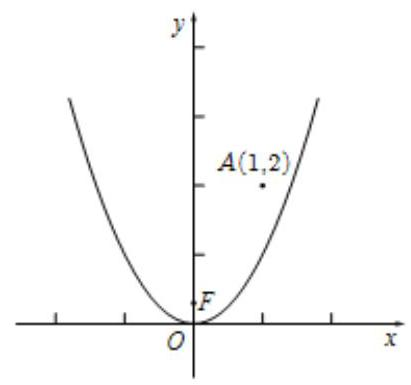
\includegraphics[max width=0.3\textwidth]{images/bo_d6dceus601uc73dvofhg_100_986_680_411_385_0.jpg}
\end{center}
\hspace*{3em} 

【答案】(1)(1，1)(-1，1) (2) \(\frac{9}{4}\) (3) \({2x} - y - 2 = 0\)

【解析】(1) 设点 \(E\) 的坐标是 \(\left( {x,y}\right)\) ,则 \(y = {x}^{2}\) . 解 \(\sqrt{{x}^{2} + {y}^{2}} = \sqrt{{x}^{2} + {x}^{4}} = \sqrt{2}\) ,得 \(x =  \pm  1\) . 因此,点 \(E\) 的坐标是 \(\left( {1,1}\right)\) 或 \(\left( {-1,1}\right)\) .

(2)设点 \(F\) 到准线的距离为 \(p\) ，则 \({2p} = 1\) ， \(p = \frac{1}{2}\) . 因此抛物线 \(\Gamma\) 的准线方程为 \(y =  - \frac{1}{4}\) . 根据抛物线定义,抛物线上点 \(P\) 到焦点 \(F\) 的距离等于到准线的距离. 过 \(P\) 作 \({PH} \bot\) 准线于 \(H\) ,过 \(A\) 作 \({AT} \bot\) 准线于 \(T\) ,则 \(\left| {AP}\right|  + \left| {PF}\right|  = \left| {AP}\right|  + \left| {PH}\right|  \geq  \left| {AT}\right|\) . 等号当 \({PA}\) 垂直于准线时取到，而 \(A\) 到准线的距离为 \(\frac{9}{4}\) ，故所求的最小值为 \(\frac{9}{4}\) .

(3)直线 \({BC}\) 的斜率存在,设为 \(k\) ,则直线 \({BC}\) 的方程为 \(y = k\left( {x - 1}\right)  + 2\) .

与 \(y = {x}^{2}\) 联立,得 \({x}^{2} - {kx} + k - 2 = 0\) .

设 \(B\left( {{x}_{1},{y}_{1}}\right) ,C\left( {{x}_{2},{y}_{2}}\right)\) ,则 \({x}_{1} + {x}_{2} = k,{x}_{1}{x}_{2} = k - 2\) .

由 \({y}^{\prime } = {2x}\) ,抛物线在 \(B\) 处的切线方程为 \(y - {x}_{1}^{2} = 2{x}_{1}\left( {x - {x}_{1}}\right)\) ,化简得 \(y = 2{x}_{1}x - {x}_{1}^{2}\) .

同理,抛物线在 \(C\) 处的切线方程为 \(y = 2{x}_{2}x - {x}_{2}^{2}\) .

联立切线方程,解得 \(D\) 的坐标为 \(\left( {\frac{k}{2},k - 2}\right)\) .

设 \(\left\{  \begin{matrix} x = \frac{k}{2}, \\  y = k - 2, \end{matrix}\right.\) 消去 \(k\) ( \(k\) 的取值范围为一切实数),得 \({2x} - y - 2 = 0\) 即为 \(D\) 的轨迹方程, 因此 \(D\) 的轨迹是一条直线. \(\searrow\)

9.【2025.12 徐汇高三一模 20】已知抛物线 \(\Gamma  : {y}^{2} = {2px}\left( {p > 0}\right)\) 的焦点为 \(F\) ,准线为 \(l\) .

(1)若点 \(E\left( {4,4}\right)\) 在抛物线 \(\Gamma\) 上，求 \({EF}\) 所在直线的斜率；

(2)若准线 \(l : x =  - 1\) ，点 \(P\) 为抛物线 \(\Gamma\) 准线 \(l\) 上的一个动点，过点 \(P\) 作圆 \(M : {x}^{2} - {4x} + {y}^{2} + 3 = 0\) 的两条切线，切点分别为 \(A\text{ 、 }B.\) 若两条切线 \({PA}\text{ 、 }{PB}\) 与 \(y\) 轴分别交于点 \(S\text{ 、 }T\) ,求 \(\left| {ST}\right|\) 的最小值;

(3) 若点 \(F\) 到准线 \(l\) 的距离为 2,过抛物线 \(\Gamma\) 的准线 \(l\) 上一点 \(Q\) 作圆 \(N : {\left( x - m\right) }^{2} + {y}^{2} = 1\left( {m > 0}\right)\) 的两条切线 \({l}_{1},{l}_{2}\) ,且 \({l}_{1},{l}_{2}\) 分别与 \(\Gamma\) 交于 \(C\left( {{s}_{1},{t}_{1}}\right) ,D\left( {{s}_{2},{t}_{2}}\right)\) 两点和 \(G\left( {{s}_{3},{t}_{3}}\right) ,H\left( {{s}_{4},{t}_{4}}\right)\) 两点. 问: 是否存在某个圆 \(N\) ,使得当点 \(Q\) 运动时, \({t}_{1}{t}_{2}{t}_{3}{t}_{4}\) 为定值? 若存在, 求出该定值; 若不存在, 请说明理由.

\begin{center}
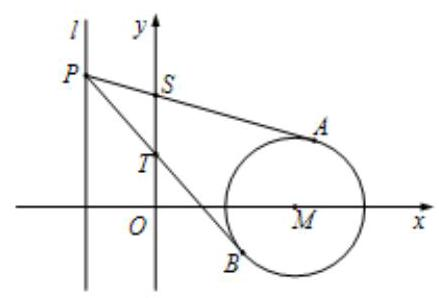
\includegraphics[max width=0.3\textwidth]{images/bo_d6dceus601uc73dvofhg_101_934_1110_439_298_0.jpg}
\end{center}
\hspace*{3em} 

【答案】(1) \(\frac{4}{3}\) (2) \(\frac{\sqrt{2}}{2}\) (3)存在

【解析】(1) 将点 \(E\left( {4,4}\right)\) 代入抛物线 \(\Gamma\) ,得 \({16} = {2p} \times  4\) ,解得 \(p = 2\) ,

所以焦点 \(F\) 的坐标为 \(\left( {1,0}\right)\) ,直线 \({EF}\) 的斜率为 \(\frac{4 - 0}{4 - 1} = \frac{4}{3}\) .

(2)设点 \(P\left( {-1,t}\right)\) ，圆 \(M\) 的切线方程为 \(y - t = k\left( {x + 1}\right)\) ，即 \({kx} - y + k + t = 0\) ，

故点 \(M\left( {2,0}\right)\) 到直线 \({kx} - y + k + t = 0\) 的距离 \(d = \frac{\left| 3k + t\right| }{\sqrt{{k}^{2} + 1}} = 1\) ,即 \(8{k}^{2} + {6kt} + {t}^{2} - 1 = 0\) ,

设直线 \({PA},{PB}\) 的斜率分别为 \({k}_{1},{k}_{2}\) ,则 \({k}_{1} + {k}_{2} =  - \frac{3t}{4},{k}_{1}{k}_{2} = \frac{{t}^{2} - 1}{8}\) ,

把 \(x = 0\) 代入 \({kx} - y + k + t = 0\) ，得 \(y = k + t\) ，

则 \(\left| {ST}\right|  = \left| {{k}_{1} + t - \left( {{k}_{2} + t}\right) }\right|  = \left| {{k}_{1} - {k}_{2}}\right|  = \sqrt{{\left( {k}_{1} + {k}_{2}\right) }^{2} - 4{k}_{1}{k}_{2}} = \sqrt{\frac{9{t}^{2}}{16} - \frac{{t}^{2} - 1}{2}} = \frac{\sqrt{{t}^{2} + 8}}{4}\) , 故当 \(t = 0\) 时, \(\left| {ST}\right|\) 取得最小值为 \(\frac{\sqrt{2}}{2}\) .

(3)法一，设点 \(Q\left( {-1,n}\right)\) ， \({l}_{1} : y = {k}_{1}\left( {x + 1}\right)  + n\) ， \({l}_{2} : y = {k}_{2}\left( {x + 1}\right)  + n\) ，显然 \({k}_{1}{k}_{2} \neq  0\) . 将 \({l}_{1}\) 方程与抛物线方程联立,消去 \(x\) 并化简可得: \({k}_{1}{y}^{2} - {4y} + 4{k}_{1} + {4n} = 0\) , 又 \(C\left( {{s}_{1},{t}_{1}}\right) ,D\left( {{s}_{2},{t}_{2}}\right)\) ,则由韦达定理可得 \({t}_{1}{t}_{2} = \frac{4{k}_{1} + {4n}}{{k}_{1}}\) ,同理可得 \({t}_{3}{t}_{4} = \frac{4{k}_{2} + {4n}}{{k}_{2}}\) . 则 \({t}_{1}{t}_{2}{t}_{3}{t}_{4} = {16} \times  \frac{{k}_{1}{k}_{2} + n\left( {{k}_{1} + {k}_{2}}\right)  + {n}^{2}}{{k}_{1}{k}_{2}} = {16}\left\lbrack  {1 + \frac{n\left( {{k}_{1} + {k}_{2}}\right)  + {n}^{2}}{{k}_{1}{k}_{2}}}\right\rbrack\) .

又 \({l}_{1}\) 与圆 \(N : {\left( x - m\right) }^{2} + {y}^{2} = 1\left( {m > 0}\right)\) 相切,则 \({l}_{1}\) 到圆心的距离为 1,

则 \(\frac{\left| {k}_{1}\left( 1 + m\right)  + n\right| }{\sqrt{{k}_{1}^{2} + 1}} = 1 \Rightarrow  \left( {{m}^{2} + {2m}}\right) {k}_{1}^{2} + {2n}\left( {m + 1}\right) {k}_{1} + {n}^{2} - 1 = 0\) ,

同理有 \(\left( {{m}^{2} + {2m}}\right) {k}_{2}^{2} + {2n}\left( {m + 1}\right) {k}_{2} + {n}^{2} - 1 = 0\) ,

则 \({k}_{1},{k}_{2}\) 为方程 \(\left( {{m}^{2} + {2m}}\right) {k}^{2} + {2n}\left( {m + 1}\right) k + {n}^{2} - 1 = 0\) 的两根.

由韦达定理可得: \({k}_{1} + {k}_{2} =  - \frac{{2n}\left( {m + 1}\right) }{m\left( {m + 2}\right) },{k}_{1}{k}_{2} = \frac{{n}^{2} - 1}{m\left( {m + 2}\right) }\) .

则 \({t}_{1}{t}_{2}{t}_{3}{t}_{4} = {16}\left\lbrack  {1 + \frac{-2{n}^{2}\left( {m + 1}\right)  + {n}^{2}\left( {m + 2}\right) m}{{n}^{2} - 1}}\right\rbrack   = {16} + {16}{n}^{2}\frac{{m}^{2} - 2}{{n}^{2} - 1}\) .

注意到当 \(n =  \pm  1\) 时,切线中有一条与 \(x\) 轴平行,不合题意,则 \({n}^{2} - 1 \neq  0\) .

要使 \({t}_{1}{t}_{2}{t}_{3}{t}_{4}\) 为定值,则 \({m}^{2} - 2 = 0\) ,又 \(m > 0\) ,则 \(m = \sqrt{2}\) .

故存在圆 \(M : {\left( x - \sqrt{2}\right) }^{2} + {y}^{2} = 1\) ,使得当点 \(N\) 运动时, \({t}_{1}{t}_{2}{t}_{3}{t}_{4}\) 为定值.

法二: 设点 \(Q\left( {-1,n}\right)\) ,若直线垂直于 \(y\) 轴,则与抛物线只有一个交点,不符题意,

故可设, \({l}_{1} : x = {r}_{1}\left( {y - n}\right)  - 1,{l}_{2} : x = {r}_{2}\left( {y - n}\right)  - 1\) ,

将 \({l}_{1}\) 方程与抛物线方程联立,消去 \(x\) 并化简可得: \({y}^{2} - 4{r}_{1}y + 4{r}_{1}n + 4 = 0\) ,

又 \(C\left( {{s}_{1},{t}_{1}}\right) ,D\left( {{s}_{2},{t}_{2}}\right)\) ,则由韦达定理可得 \({t}_{1}{t}_{2} = 4{r}_{1}n + 4\) ,同理可得 \({t}_{3}{t}_{4} = 4{r}_{2}n + 4\) ,

则 \({t}_{1}{t}_{2}{t}_{3}{t}_{4} = \left( {4{r}_{1}n + 4}\right) \left( {4{r}_{2}n + 4}\right)  = {16}\left\lbrack  {{n}^{2}{r}_{1}{r}_{2} + n\left( {{r}_{1} + {r}_{2}}\right)  + 1}\right\rbrack\) ,

又 \({l}_{1}\) 与圆 \(N : {\left( x - m\right) }^{2} + {y}^{2} = 1\left( {m > 0}\right)\) 相切,则 \({l}_{1}\) 到圆心的距离为 1,则 \(\frac{\left| m + {r}_{1}n + 1\right| }{\sqrt{{r}_{1}^{2} + 1}} = 1\) ,整理得

\(\left( {{n}^{2} - 1}\right) {r}_{1}^{2} + 2\left( {m + 1}\right) n{r}_{1} + {m}^{2} + {2m} = 0,\)

同理有 \(\left( {{n}^{2} - 1}\right) {r}_{2}^{2} + 2\left( {m + 1}\right) n{r}_{2} + {m}^{2} + {2m} = 0\) ,

则 \({r}_{1},{r}_{2}\) 为方程 \(\left( {{n}^{2} - 1}\right) {r}^{2} + 2\left( {m + 1}\right) {nr} + {m}^{2} + {2m} = 0\) 的两根,

由韦达定理可得, \({r}_{1} + {r}_{2} =  - \frac{2\left( {m + 1}\right) n}{{n}^{2} - 1},{r}_{1}{r}_{2} = \frac{{m}^{2} + {2m}}{{n}^{2} - 1}\) ,

则 \({t}_{1}{t}_{2}{t}_{3}{t}_{4} = {16}\left\lbrack  {{n}^{2} \cdot  \frac{{m}^{2} + {2m}}{{n}^{2} - 1} - \frac{2\left( {m + 1}\right) {n}^{2}}{{n}^{2} - 1} + 1}\right\rbrack   = {16} + {16}{n}^{2} \cdot  \frac{{m}^{2} - 2}{{n}^{2} - 1}\) .

注意到当 \(n =  \pm  1\) 时,切线中有一条与 \(x\) 轴平行,不合题意,则 \({n}^{2} - 1 \neq  0\) . 要使 \({t}_{1}{t}_{2}{t}_{3}{t}_{4}\) 为定值,则 \({m}^{2} - 2 = 0\) ,又 \(m > 0\) ,则 \(m = \sqrt{2}\) .

故存在圆 \(M : {\left( x - \sqrt{2}\right) }^{2} + {y}^{2} = 1\) ,使得当点 \(N\) 运动时, \({t}_{1}{t}_{2}{t}_{3}{t}_{4}\) 为定值. \(>\)

\section*{7.5 新定义}

1.【2025.12 黄浦高三一模 12】若图形 \(\Gamma\) 上的每个点都在圆 \(C\) 上或在圆 \(C\) 内部,则称圆 \(C\) 为 \(\Gamma\) 的一个覆盖圆. 设 \(\Gamma\) 由函数 \(y = 2\left| x\right|  - 4\left( {-2 < x < 2}\right)\) 与 \(y = \sqrt{2\left| x\right|  - {x}^{2}}\) 的图像所组成, 则 \(\Gamma\) 的最小覆盖圆的半径为\_\_\_\_\_.

【答案】 \(\frac{8}{3}\)

【解析】分别画出 \(y = 2\left| x\right|  - 4\left( {-2 < x < 2}\right)\) 与 \(y = \sqrt{2\left| x\right|  - {x}^{2}}\) 的图像,如下图所示: 根据对称性,可知最小覆盖圆与左右两个半圆外切,且圆心必定在 \(y\) 轴上,设半径为 \(R\) . 则有 \({\left( 4 - R\right) }^{2} + {1}^{2} = {\left( R - 1\right) }^{2}\) ,解得 \(R = \frac{8}{3}\) .

\begin{center}
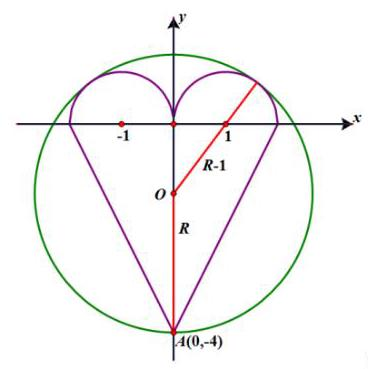
\includegraphics[max width=0.3\textwidth]{images/bo_d6dceus601uc73dvofhg_104_1004_804_368_369_0.jpg}
\end{center}
\hspace*{3em} 

2.【2025.12 松江高三一模 16】定义:一个平面封闭区域内任意两点之间的距离的最大值称为该区域的“直径”. 在 \(\bigtriangleup  {ABC}\) 中， \({BC} = 1\) ， \({BC}\) 边上的高等于 \(\tan A\) ，以 \(\bigtriangleup  {ABC}\) 的各边为直径向 \(\bigtriangleup  {ABC}\) 外分别作三个半圆，记三个半圆围成的平面区域的“直径”为 \(d\) ，则以下两个结论:

 \circled{1}  当 \(\angle {ABC} = \frac{\pi }{2}\) 时， \(d = \frac{\sqrt{2} + 2}{2}\) ； \circled{2}  \(d\) 的最大值为 \(\frac{\sqrt{6} + 1}{2}\) ( ) .

A.  \circled{1} 正确， \circled{2} 错误 B.  \circled{1}  \circled{2} 都正确

C.  \circled{1} 错误， \circled{2} 正确 D.  \circled{1}  \circled{2} 都错误

【答案】B

【解析】对命题 \circled{1} :设 \({AB} = c,{AC} = b\) ，当 \({\angle {ABC}} = \frac{\pi }{2}\) 时，可得 \(c = \tan A\) ，从而可知: \(c = a = 1\) ,即此时 \(\bigtriangleup {ABC}\) 为等腰直角三角形.

如图 16-1 所示,设 \({AB},{AC}\) 的中点分别为 \(M,N\) .

根据对称性可知: 此时 “直径” \(d = {PQ} = {MN} + {r}_{1} + {r}_{2} = \frac{a}{2} + \frac{b}{2} + \frac{c}{2} = \frac{\sqrt{2} + 2}{2}\) ，故命题 \circled{1} 为真命题;

\begin{center}
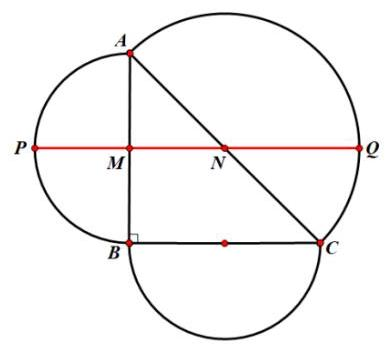
\includegraphics[max width=0.3\textwidth]{images/bo_d6dceus601uc73dvofhg_105_392_199_388_349_0.jpg}
\end{center}
\hspace*{3em} 

图 16-1

\begin{center}
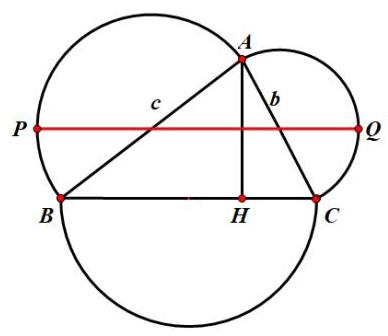
\includegraphics[max width=0.3\textwidth]{images/bo_d6dceus601uc73dvofhg_105_854_205_388_336_0.jpg}
\end{center}
\hspace*{3em} 

图 16-2

对命题 \circled{2} :如图 16-2 所示，设 \({AB} = c,{AC} = b\) ，由面积公式得

\({S}_{\bigtriangleup {ABC}} = \frac{1}{2}{bc}\sin A = \frac{1}{2}{BC} \cdot  \tan A\) ,化简得 \({bc} = \frac{1}{\cos A}\) .

又由余弦定理得 \({b}^{2} + {c}^{2} - {2bc}\cos A = B{C}^{2} = 1\) ,化简得 \({b}^{2} + {c}^{2} = 3\) . 再由 \(2\left( {{b}^{2} + {c}^{2}}\right)  \geq  {\left( b + c\right) }^{2}\)

得 \(b + c \leq  \sqrt{6}\) ,此时 “直径” \(d = {PQ} = \frac{a}{2} + \frac{b}{2} + \frac{c}{2} \leq  \frac{1 + \sqrt{6}}{2}\) ,故命题 \circled{2} 也为真命题.

3.【2025.12 金山高三一模 16】记曲线 \(C : \frac{{\left| x\right| }^{n}}{a} + \frac{{\left| y\right| }^{n}}{b} = 1\left( {a > 0\text{ 且 }b > 0,n > 0\text{ 且 }n \in  \mathbf{R}}\right)\) 为 \({C}_{\left( a,b\right) }^{n}\) , 称其为“超椭圆”. 命题 \(p\) : 直线 \(l : {2x} + {9y} - {12} = 0\) 与超椭圆 \({C}_{\left( 3,2\right) }^{\frac{1}{2}}\) 有 3 个不同交点；命题 \(q\) : 超椭圆 \({C}_{\left( 9,1\right) }^{8}\) 上的点到坐标原点距离的取值范围为 \(\left\lbrack  {1,{2}^{\frac{5}{8}}}\right\rbrack\) . 则下列说法正确的是 ( )

A. 命题 \(p\) 为 A 命题,命题 \(q\) 为假命题 B. 命题 \(p\) 为假命题,命题 \(q\) 为真命题

C. 命题 \(p\text{ 、 }q\) 均为真命题 D. 命题 \(p\text{ 、 }q\) 均为假命题

【答案】A

【解析】解法一 (几何角度):

对命题 \circled{1} :超椭圆 \({C}_{\left( 3,2\right) }^{\frac{1}{2}}\) 的方程为 \(\frac{\sqrt{\left| x\right| }}{3} + \frac{\sqrt{\left| y\right| }}{2} = 1\) ,图像分别关于 \(x,y\) 轴对称,分别画出椭圆 \({C}_{\left( 3,2\right) }^{\frac{1}{2}}\) 和直线 \(l\) 的图像,如图 16-1 所示:

\begin{center}
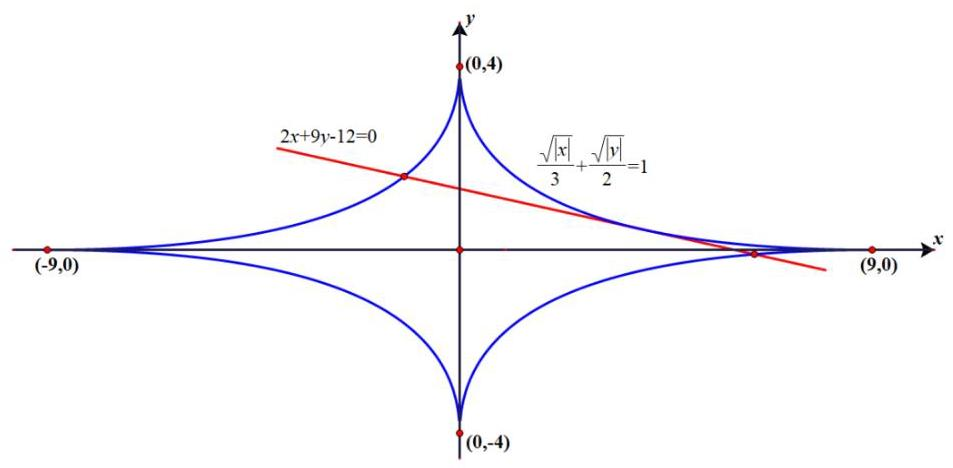
\includegraphics[max width=0.8\textwidth]{images/bo_d6dceus601uc73dvofhg_106_351_203_953_468_0.jpg}
\end{center}
\hspace*{3em} 

图 16-1

不难发现直线 \(l : {2x} + {9y} - {12} = 0\) 与超椭圆 \({C}_{\left( 3,2\right) }^{\frac{1}{2}}\) 在第一象限内刚好相切，外加第二象限和第四象限各 1 个交点, 总共 3 个公共点, 故 \circled{1} 为真命题;

对命题 \circled{2} :此时超椭圆为 \(\frac{{\left| x\right| }^{8}}{9} + {\left| y\right| }^{8} = 1\) ，根据对称性，只需考虑第一象限内的图像，如图 16- 2 所示.

再以 \(r = {2}^{\frac{5}{8}}\) 画圆,与超椭圆并没有交点,即超椭圆 \({C}_{\left( 9,1\right) }^{8}\) 上的点到坐标原点的最大距离是小于 \(r = {2}^{\frac{5}{8}}\) ,故命题 \circled{2} 为假命题.

\begin{center}
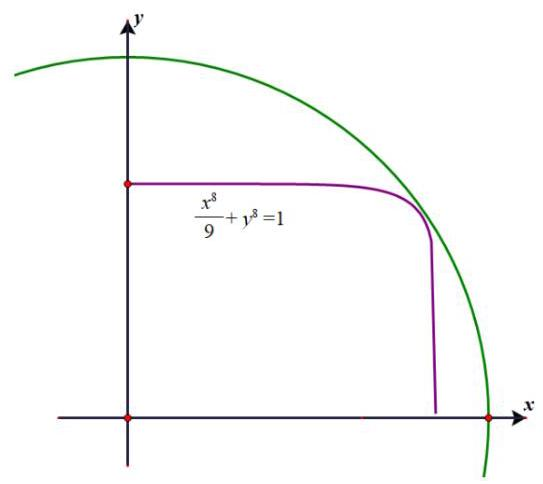
\includegraphics[max width=0.4\textwidth]{images/bo_d6dceus601uc73dvofhg_106_552_1263_543_484_0.jpg}
\end{center}
\hspace*{3em} 

图 16-2

解法二 (代数思路):

对命题 \circled{1} :超椭圆 \({C}_{\left( 3,2\right) }^{\frac{1}{2}}\) 在第一象限内的方程为 \(\frac{\sqrt{x}}{3} + \frac{\sqrt{y}}{2} = 1\) .

联立 \(\left\{  \begin{array}{l} \frac{\sqrt{x}}{3} + \frac{\sqrt{y}}{2} = 1 \\  {2x} + {9y} - {12} = 0 \end{array}\right.\) ,设 \(\left\{  \begin{array}{l} \sqrt{x} = m \\  \sqrt{y} = n \end{array}\right.\) ,即 \(\left\{  \begin{array}{l} \frac{m}{3} + \frac{n}{2} = 1 \\  2{m}^{2} + 9{n}^{2} - {12} = 0 \end{array}\right.\) 得 \({m}^{2} - {4m} + 4 = 0\) ,

解得 \(\left\{  \begin{array}{l} m = 2 \\  n = \frac{2}{3} \end{array}\right.\) ,即 \(\left\{  \begin{array}{l} x = 4 \\  y = \frac{4}{9} \end{array}\right.\) ,也即超椭圆 \({C}_{\left( 3,2\right) }^{\frac{1}{2}}\) 与直线 \(l : {2x} + {9y} - {12} = 0\) 在第一象限内只有唯一交点 \(\left( {4,\frac{4}{9}}\right)\) ,所以直线 \(l : {2x} + {9y} - {12} = 0\) 与超椭圆 \({C}_{\left( 3,2\right) }^{\frac{1}{2}}\) 在第一象限内刚好相切于点 \(\left( {4,\frac{4}{9}}\right)\) .

加上第二象限和第四象限各 1 个交点,总共 3 个公共点,故 \circled{1} 为真命题;

对命题 \circled{2} :此时超椭圆为 \(\frac{{\left| x\right| }^{8}}{9} + {\left| y\right| }^{8} = 1\) ，根据对称性，只考虑第一象限内的解析式:

\(\frac{{x}^{8}}{9} + {y}^{8} = 1\) . 联立 \(\left\{  \begin{array}{l} \frac{{x}^{8}}{9} + {y}^{8} = 1 \\  {x}^{2} + {y}^{2} = {2}^{\frac{5}{4}} \end{array}\right.\) ,设 \(\left\{  {\begin{array}{l} {x}^{2} = m \\  {y}^{2} = n \end{array}\left( {m,n > 0}\right) }\right.\) ,得 \(\left\{  \begin{array}{l} \frac{{m}^{4}}{9} + {n}^{4} = 1 \\  m + n = {2}^{\frac{5}{4}} \end{array}\right.\) ,

借助计算器解得该方程组无解, \(\therefore\) 命题 \circled{2} 为假命题. \(\propto\)

\section*{7.6 曲线方程}

1.【2025.12 崇明高三一模 15】已知 \(A\text{ 、 }B\) 为平面内两定点，过该平面内动点 \(M\) 作直线 \({AB}\) 的垂线,垂足为 \(N\) . 若 \({\overrightarrow{MN}}^{2} = \lambda \overrightarrow{AN} \cdot  \overrightarrow{NB}\) ,其中 \(\lambda\) 为常数,则动点 \(M\) 的轨迹不可能是( )

A. 圆 B. 椭圆 C. 抛物线 D. 双曲线

【答案】C

【解析】以线段 \({AB}\) 所在直线为 \(x\) 轴,以其中垂线为 \(y\) 轴,建系.

不妨设 \({AB} = {2a}\) ,则 \(A\left( {-a,0}\right) ,B\left( {a,0}\right)\) . 设 \(M\left( {x,y}\right)\) ,则 \(N\left( {x,0}\right)\) .

由 \({\overrightarrow{MN}}^{2} = \lambda \overrightarrow{AN} \cdot  \overrightarrow{NB}\) 得 \({\left( 0, - y\right) }^{2} = \lambda \left( {x + a,0}\right)  \cdot  \left( {a - x,0}\right)\) ,整理得 \(\lambda {x}^{2} + {y}^{2} = \lambda {a}^{2}\) .

当 \(\lambda  = 1\) 时,动点 \(M\) 的轨迹方程为 \({x}^{2} + {y}^{2} = {a}^{2}\) ,是一个圆,排除 \(\mathrm{A}\) ;

当 \(\lambda  \in  \left( {0,1}\right)  \cup  \left( {1, + \infty }\right)\) 时,动点 \(M\) 的轨迹方程为 \(\frac{{x}^{2}}{{a}^{2}} + \frac{{y}^{2}}{\lambda {a}^{2}} = 1\) ,是一个椭圆,排除 \(\mathrm{B}\) ;

当 \(\lambda  \in  \left( {-\infty ,0}\right)\) 时,动点 \(M\) 的轨迹方程为 \(\frac{{x}^{2}}{{a}^{2}} - \frac{{y}^{2}}{-\lambda {a}^{2}} = 1\) ,是一个双曲线,排除 \(\mathrm{D}\) ;

所以选 C. \(\ll\)

2.【 2025.12 奉贤高三一模 15】曲线 \(C\) 的方程为 \(A{x}^{2} - B{y}^{2} = {\lambda }^{2}\) ( \(A\) 、 \(B\) 不同时为 0 )，则下列说法正确的是( )

A. 曲线 \(C\) 不可能是直线

B. 当 \(A > 0,B < 0\) 时,曲线是椭圆

C. 若曲线 \(C\) 是双曲线,则双曲线的渐近线与 \(\lambda\) 无关

D. 曲线 \(C\) 是抛物线

【答案】C

【解析】当该方程表示双曲线时,其渐近线方程为 \(A{x}^{2} - B{y}^{2} = 0\) ,即 \(y =  \pm  \sqrt{\frac{B}{A}}x\) ,确实与 \(\lambda\) 的取值无关，故选 C. \(\ll\)

\section*{第八章 立体几何}

\section*{【知识概要】}

1、如果一个角的两边分别与另一个角的两边平行，那么这两个角相等或互补。

2、空间直线所成角范围是 \(\left\lbrack  {0,\frac{\pi }{2}}\right\rbrack\) 。

空间直线 \(l\) 与平面 \(\alpha\) 所成角范围是 \(\left\lbrack  {0,\frac{\pi }{2}}\right\rbrack\) 。

空间平面 \({\alpha }_{1}\) 与平面 \({\alpha }_{2}\) 所成角范围是 \(\lbrack 0,\pi )\) 。

3、线面垂直面面垂直判定定理!

4、在平面内的一条直线, 如果它和这个平面的一条斜线的射影垂直, 那么它也和这条斜线垂直

平面内的一条直线, 如果和这个平面的一条斜线垂直, 那麽它也和这条斜线的射影垂直。

5、斜二测法规定在 x 轴方向上线段的长度是其表示的真实长度的一半，在 y 轴和 z 轴方向上线段的长度与其表示的真实长度相等。

斜二测画法中原图形和直观图的面积比为1: \(\frac{\sqrt{2}}{4}\) 。

6、祖暅原理是:体积可以看成是由面积叠加而成，用一组平行平面截两个空间图形，若在任意等高处的截面面积都对应相等，则两空间图形的体积相等。

7、设几何体的底面周长为 \(\mathrm{C}\) ,母线或斜高长为 \({h}^{\prime }\) ,则圆柱或直棱柱的侧面积为 \(C{h}^{\prime }\) ; 圆锥或正棱锥的侧面积为 \(\frac{1}{2}C{h}^{\prime }\) ; 半径为 \(\mathrm{R}\) 的球的表面积为 \({4\pi }{R}^{2}\) 。

8、柱体体积公式为 \({Sh}\) ，锥体体积公式为 \(\frac{1}{3}{Sh}\) ，半径为 \(\mathrm{R}\) 的球的体积为 \(\frac{4}{3}\pi {R}^{3}\) 。

9、半径为 \(\mathrm{R}\) 的球的小圆半径为 \(r = \sqrt{{R}^{2} - {d}^{2}}\) (球心到小圆所在平面距离为 \(\mathrm{d}\) )

10、球面距离是指联结球面上两点的路径中，通过该两点的大圆劣弧的长度。

11. 空间向量公式:

已知空间中，直线 \({l}_{1}\) ， \({l}_{2}\) 方向向量分别为 \(\overrightarrow{{d}_{1}}\) ， \(\overrightarrow{{d}_{2}}\) ，平面 \(\alpha\) 、 \(\beta\) 分别法向量为 \(\overrightarrow{{n}_{1}}\) ， \(\overrightarrow{{n}_{2}}\) ，

则直线 \({l}_{1}\) 与 \({l}_{2}\) 所成角 \(\theta\) 满足: \(\cos \theta  = \left| \frac{\overrightarrow{{d}_{1}} \cdot  \overrightarrow{{d}_{2}}}{\left| \overrightarrow{{d}_{1}}\right| \left| \overrightarrow{{d}_{2}}\right| }\right|\)

直线 \({l}_{1}\) 与平面 \(\alpha\) 所成角 \(\theta\) 满足: \(\sin \theta  = \left| \frac{\overrightarrow{{d}_{1}} \cdot  \overrightarrow{{n}_{1}}}{\left| \overrightarrow{{d}_{1}}\right| \left| \overrightarrow{{n}_{1}}\right| }\right|\)

平面 \(\alpha\) 与平面 \(\beta\) 所成二面角 \(\theta\) 满足: \(\cos \theta  = \frac{\overrightarrow{{n}_{1}} \cdot  \overrightarrow{{n}_{2}}}{\left| \overrightarrow{{n}_{1}}\right| \left| \overrightarrow{{n}_{2}}\right| }\) 或 \(\cos \theta  = \frac{\overrightarrow{{n}_{1}} \cdot  \overrightarrow{{n}_{2}}}{\left| \overrightarrow{{n}_{1}}\right| \left| \overrightarrow{{n}_{2}}\right| }\) 点 \(\mathrm{A}\) 到平面 \(\alpha\) 的距离 \(\mathrm{d} = \left| \frac{\overrightarrow{AM} \cdot  \overrightarrow{{n}_{1}}}{\left| \overrightarrow{{n}_{1}}\right| }\right|\)

\section*{8.1 位置关系}

1.【2025.12 奉贤高三一模 7】在正四棱台 \({ABCD} - {A}_{1}{B}_{1}{C}_{1}{D}_{1}\) 中，异面直线 \(A{A}_{1}\) 与 \({D}_{1}{B}_{1}\) 所成角的大小为\_\_\_\_\_.

【答案】 \({90}^{ \circ  }\)

【解析】依题意可得: \({B}_{1}{D}_{1} \bot\) 平面 \(A{A}_{1}{C}_{1}C,\therefore {B}_{1}{D}_{1} \bot  A{A}_{1}\) ,即二者所成角为 \({90}^{ \circ  }\) . \(<\)

2.【2025.12 普陀高三一模 8】在 \(\bigtriangleup {ABC}\) 中， \(A = \frac{\pi }{3}\) ， \({AB} = 2\) ， \({AC} = 5\) ， \(D\) 为 \({AC}\) 边上的一点，且 \({AD} = 2\) ，现将 \(\bigtriangleup  {ABD}\) 沿 \({BD}\) 边折起，使得点 \(A\) 至点 \(P\) 的位置，且满足平面 \({PBD}\bot\) 平面 \({BDC}\) ，如图所示，则直线 \({PC}\) 与平面 \({BDC}\) 所成的角的正弦值为\_\_\_\_\_.

\begin{center}
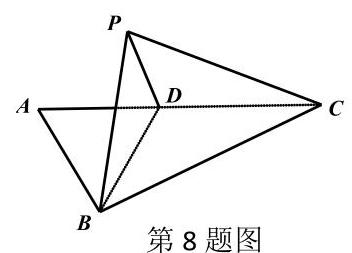
\includegraphics[max width=0.3\textwidth]{images/bo_d6dceus601uc73dvofhg_110_491_1047_352_253_0.jpg}
\end{center}
\hspace*{3em} 

\begin{center}
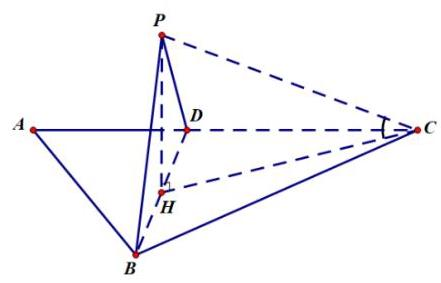
\includegraphics[max width=0.3\textwidth]{images/bo_d6dceus601uc73dvofhg_110_957_1039_441_283_0.jpg}
\end{center}
\hspace*{3em} 

【答案】 \(\sin \angle {PCH} = \frac{\sqrt{3}}{4}\) .

【解析】取 \({BD}\) 中点 \(H\) ,联结 \({PH}\) . 在等边 \(\bigtriangleup {PBD}\) 中,易得 \({PH} \bot  {BD}\) .

根据平面 \({PBD} \bot\) 平面 \({BCD}\) 且平面 \({PBD} \cap\) 平面 \({BCD} = {BD},\therefore {PH} \bot\) 平面 \({BCD}\) ,所以 \(\angle {PCH}\) 即为直线 \({PC}\) 与平面 \({BCD}\) 所成角.

在 \({\Delta CDH}\) 中, \({CD} = 5,{DH} = 1,\angle {CDH} = {120}^{ \circ  }\) ,由余弦定理得 \({CH} = \sqrt{13}\) ,而 \({PH} = \sqrt{3}\) ,所以 \({PC} = \sqrt{P{H}^{2} + C{H}^{2}} = 4,\therefore \sin \angle {PCH} = \frac{PH}{PC} = \frac{\sqrt{3}}{4} \cdot  8 <\)

3.【2025.12 宝山高三一模 11】如图，点 \(P\) 在圆柱 \({O}_{1}O\) 的底面圆 \(O\) 的圆周上， \({AB}\) 为圆 \(O\) 的直径, \(\angle {AOP} = {120}^{ \circ  },{OA} = 3,{A}_{1}B\) 与底面圆 \(O\) 所成的角为 \({30}^{ \circ  }\) ,则异面直线 \({A}_{1}B\) 与 \({AP}\) 所成角的余弦值为\_\_\_\_\_.

\begin{center}
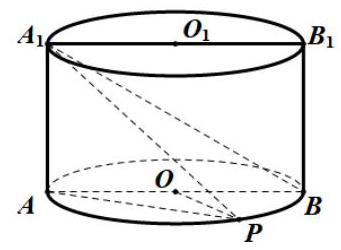
\includegraphics[max width=0.2\textwidth]{images/bo_d6dceus601uc73dvofhg_111_446_469_341_250_0.jpg}
\end{center}
\hspace*{3em} 

\begin{center}
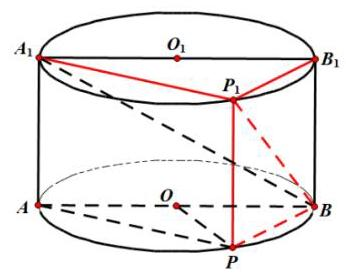
\includegraphics[max width=0.2\textwidth]{images/bo_d6dceus601uc73dvofhg_111_847_451_346_274_0.jpg}
\end{center}
\hspace*{3em} 

【答案】 \(\frac{3}{4}\)

【解析】依题意可得: \(\angle {A}_{1}{BA} = {30}^{ \circ  },\angle {BAP} = {30}^{ \circ  }\) .

\(\therefore {A}_{1}A = {AB}\tan {30}^{ \circ  } = 2\sqrt{3},{AP} = {AB}\cos {30}^{ \circ  } = 3\sqrt{3},{BP} = {AB}\sin {30}^{ \circ  } = 3\) .

作 \(P{P}_{1} \bot\) 上底圆 \({O}_{1}\) ,交圆弧 \(\overset{\text{ ⏜ }}{{A}_{1}{B}_{1}}\) 于点 \({P}_{1}\) ,联结 \({A}_{1}{P}_{1},{B}_{1}{P}_{1},B{P}_{1}\) ,则 \({A}_{1}{P}_{1}//{AP},\therefore \angle B{A}_{1}{P}_{1}\) 为异面直线 \({A}_{1}B\) 与 \({AP}\) 所成角.

易得 \({A}_{1}{P}_{1} \bot\) 平面 \({PB}{B}_{1}{P}_{1},\therefore {A}_{1}{P}_{1} \bot  B{P}_{1}\) .

在 \({Rt\Delta B}{A}_{1}{P}_{1}\) 中， \({A}_{1}{P}_{1} = {AP} = 3\sqrt{3}\) ， \({A}_{1}B = \frac{AB}{\cos {30}^{ \circ  }} = 4\sqrt{3}\) ，可得 \(\cos \angle B{A}_{1}{P}_{1} = \frac{{A}_{1}{P}_{1}}{{A}_{1}B} = \frac{3}{4}\) ，

所以异面直线 \({A}_{1}B\) 与 \({AP}\) 所成角的余弦值为 \(\frac{3}{4}\) .

4.【2025.12 青浦高三一模 13】在空间中，“两条直线平行”是“两条直线没有公共点”的( ).

A. 充分不必要条件 B. 必要不充分条件

C. 充要条件 D. 既非充分也不必要条件

【答案】A※

5.【2025.12 静安高三一模 13】在三维空间中，下列命题是真命题的是( ).

A. 垂直于同一条直线的两条直线平行

B. 垂直于同一个平面的两个平面平行

C. 若一条直线垂直于一个平面, 另一条直线与这个平面平行, 则这两条直线互相垂直

D. 若两个平面分别平行于两条互相垂直的直线, 则这两个平面互相垂直

【答案】C <

6.【2025.12 长宁高三一模 13】如图,已知 \(A,B,C,D,E,F,G\) 分别是正方体所在棱的中点,则下列直线中与直线 \({EF}\) 异面的是( )

A. 直线 \({AB}\) ； B. 直线 \({AC}\) ； C. 直线 \({AG}\) : D. 直线 \({AG}\) .

\begin{center}
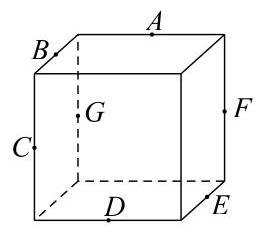
\includegraphics[max width=0.2\textwidth]{images/bo_d6dceus601uc73dvofhg_112_1128_430_259_229_0.jpg}
\end{center}
\hspace*{3em} 

【答案】D. \(\ll\)

7.【2025.12 松江高三一模 13】若空间中三条不同的直线 \(a,b,c\) 满足 \(a \bot  c,b \bot  c\) ,则 “ \(a//b\) ”是“ \(a,b,c\) 共面”的( )

A. 充分非必要条件 B. 必要非充分条件

C. 充要条件 D. 既非充分又非必要条件

【答案】B《

8.【2025.12 浦东高三一模 13】已知直线 \(a\text{ 、 }b\) 和平面 \(\alpha \text{ 、 }\beta\) ，且 \(a \subseteq  \alpha \text{ 、 }b \subseteq  \beta\) ，则“ \(a\) 与 \(b\) 相交”是 “ \(\alpha\) 与 \(\beta\) 相交” 的( )

A. 充分必要条件 B. 既不充分又不必要条件

C. 充分不必要条件 D. 必要不充分条件

【答案】C <

9.【2025.12 黄浦高三一模 14】设 \(\alpha ,\beta\) 是两个不同的平面， \(l\) 是一条直线，以下命题正确的是( )

A. 若 \(l \bot  \alpha ,\alpha  \bot  \beta\) ,则 \(l//\beta\) B. 若 \(l//\alpha ,\alpha //\beta\) ,则 \(l//\beta\)

C. 若 \(l \bot  \alpha ,\alpha //\beta\) ,则 \(l \bot  \beta\) D. 若 \(l//\alpha ,\alpha  \bot  \beta\) ,则 \(l \bot  \beta\)

【答案】C

【答案】 \(\mathrm{A}/\mathrm{B}\) 选项中,均有可能 \(l//\beta\) 或 \(l \subset  \beta\) ;

D 中可能得结果有 \(l \bot  \beta\) 或 \(l \subset  \beta\) 或 \(l\) 与 \(\beta\) 斜交,只有 \(\mathrm{C}\) 正确. \(\gg\)

10.【2025.12 奉贤高三一模 14】设 \(\alpha \text{ 、 }\beta \text{ 、 }\gamma\) 是互不重合的平面， \(m\text{ 、 }n\) 是互不重合的直线,给出四个命题:

 \circled{1} 若 \(m//\alpha ,m//\beta\) ，则 \(\alpha //\beta\)  \circled{2} 若 \(\alpha  \bot  \gamma ,\beta  \bot  \gamma\) ，则 \(\alpha  \bot  \beta\)

 \circled{3} 若 \(m \bot  \alpha ,m \bot  \beta\) ，则 \(\alpha //\beta\)  \circled{4} 若 \(m//\alpha ,n \bot  \alpha\) ，则 \(m \bot  n\)

其中正确命题的个数是( )

A. 1 B. 2 C. 3 D. 4

【答案】B

\section*{【解析】只有 \circled{3}  \circled{4} 两个命题正确, 故选 B.J.≈}

11.【2025.12 杨浦高三一模 14】若 \(m,n\) 为两条不同直线， \(\alpha ,\beta\) 为两个不同平面，则下列结论中正确的是( ).

A. 若 \(m//\alpha ,n \subset  \alpha\) ,则 \(m//n\) B. 若 \(m//n,n \subset  \alpha\) ,则 \(m//\alpha\)

C. 若 \(m \subset  \alpha ,m \bot  \beta\) ,则 \(\alpha  \bot  \beta\) D. 若 \(m \subset  \alpha ,\alpha  \bot  \beta\) ,则 \(m \bot  \beta\)

【答案】C

【解析】由面面垂直的判定定理可知: \(\mathrm{C}\) 正确. \(>\)

12.【2025.12 普陀高三一模 14】已知直线 \(m\text{ 、 }l\) 和平面 \(\alpha \text{ 、 }\beta\) ，且 \(l \subset  \alpha ,\alpha //\beta\) ，则下列命题中正确的是 ( ) .

A. 若 \(m//\beta\) ,则 \(m//l\) B. 若 \(m//l\) ，则 \(m//\alpha\)

C. 若 \(m \bot  \beta\) ，则 \(m \bot  l\) D. 若 \(m \bot  l\) ,则 \(m \bot  \alpha\)

【答案】C

【解析】当 \(m \bot  \beta\) 且 \(\alpha //\beta\) 时, \(m \bot  \alpha\) ,再结合 \(l \subset  \alpha\) ,可得 \(m \bot  l\) ,故选 C. \(\ll\)

13.【2025.12 虹口高三一模 15】如图,已知点 \(A,B,C,D\) 在表面积为 \({12\pi }\) 的球 \(O\) 的球面上, 且 \(O \in  {BD},{OA} \bot\) 平面 \({BCD}\) ,点 \(E\) 为 \({BC}\) 中点,当二面角 \(A - {BC} - D\) 的大小为 \(\frac{\pi }{3}\) 时,则有 ( )

A. 异面直线 \({EA}\) 和 \({CD}\) 所成角的大小为 \(\frac{\pi }{6}\)

B. 直线 \({EA}\) 与平面 \({ABD}\) 所成角的大小为 \(\frac{\pi }{6}\)

C. \(\sin \left( {2\angle {ABE}}\right)  = \frac{\sqrt{2}}{3}\)

D. \(\bigtriangleup {BED}\) 的面积为 \(\sqrt{2}\)

\begin{center}
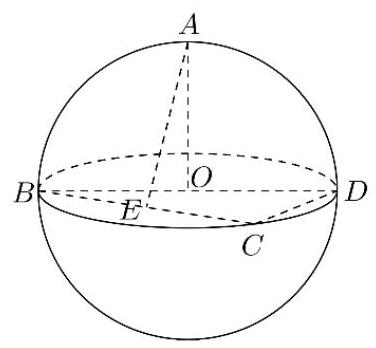
\includegraphics[max width=0.3\textwidth]{images/bo_d6dceus601uc73dvofhg_114_418_194_376_348_0.jpg}
\end{center}
\hspace*{3em} 

\begin{center}
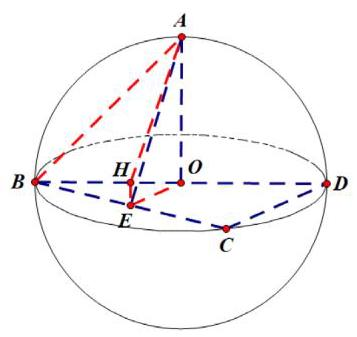
\includegraphics[max width=0.3\textwidth]{images/bo_d6dceus601uc73dvofhg_114_879_204_357_337_0.jpg}
\end{center}
\hspace*{3em} 

【答案】D

【解析】A 选项: 联结 \({OD}\) ,则 \({AE} \bot  {BC},{OE} \bot  {BC},\therefore \angle {AEO}\) 是二面角 \(A - {BC} - D\) 的平面角. 由 \(E\) 为 \({BC}\) 中点得 \({OE}//{CD}\) ,异面直线 \({EA}\) 和 \({CD}\) 所成角为线 \({EA}\) 和 \({EO}\) 所成角,

即 \(\angle {AEO}\) ,大小为 \(\frac{\pi }{3},\mathrm{\;A}\) 选项错;

B 选项: 作 \({EH} \bot  {BD}\) 于点 \(H\) ,联结 \({AH}\) ,则易得 \(\angle {EAH}\) 直线 \({EA}\) 与平面 \({ABD}\) 所成角.

又易得球 \(O\) 的半径为 \(R = {OA} = \sqrt{3},\therefore {OE} = 1,{AE} = 2\) ,且可得 \({EH} = \frac{\sqrt{6}}{3}\) .

所以 \(\sin \angle {EAH} = \frac{EH}{AE} = \frac{\sqrt{6}}{6},\mathrm{\;B}\) 选项错;

C 选项: \({AE} = 2,{BE} = \sqrt{2},{AB} = \sqrt{2}{OA} = \sqrt{6},\therefore \sin \angle {ABE} = \frac{AE}{AB} = \frac{2}{\sqrt{6}}\) ,

\(\cos \angle {ABE} = \frac{BE}{AB} = \frac{\sqrt{2}}{\sqrt{6}},\therefore \sin \left( {2\angle {ABE}}\right)  = \frac{2\sqrt{2}}{3},\mathrm{C}\) 选项错；

D 选项: 易得 \({S}_{\bigtriangleup {BED}} = 2{S}_{\bigtriangleup {BEO}} = 2 \times  \frac{1}{2} \times  {EO} \cdot  {BE} = \sqrt{2}\) ，D 选项对，选 D.e \&

\section*{8.2 空间向量}

1.【2025.12 嘉定高三一模 5】已知空间向量 \(\overrightarrow{a}\bot \overrightarrow{b},\overrightarrow{a}\bot \overrightarrow{c},\overrightarrow{b}\bot \overrightarrow{c}\) ,且 \(\left| \overrightarrow{a}\right|  = \left| \overrightarrow{b}\right|  = \left| \overrightarrow{c}\right|  = 1\) ,则 \(\left| {\overrightarrow{a} + \overrightarrow{b} + \overrightarrow{c}}\right|  =\) \_\_\_\_\_.

【答案】 \(\sqrt{3}\)

【解析】 \(\left| {\overrightarrow{a} + \overrightarrow{b} + \overrightarrow{c}}\right|  = \sqrt{{\left( \overrightarrow{a} + \overrightarrow{b} + \overrightarrow{c}\right) }^{2}} = \sqrt{{\overrightarrow{a}}^{2} + {\overrightarrow{b}}^{2} + {\overrightarrow{c}}^{2}} = \sqrt{3}\) . \(\propto\)

2.【2025.12 青浦高三一模 8】如图，在四面体 \({OABC}\) 中， \(D\) 为 \({BC}\) 的中点， \(3\overrightarrow{AG} = 2\overrightarrow{AD}\) ，且 \(P\) 为 \({OG}\) 的中点,设 \(\overrightarrow{OA} = \overrightarrow{a},\overrightarrow{OB} = \overrightarrow{b},\overrightarrow{OC} = \overrightarrow{c}\) ,用 \(\overrightarrow{a},\overrightarrow{b},\overrightarrow{c}\) 表示 \(\overrightarrow{OP}\) ,则 \(\overrightarrow{OP} =\) \_\_\_\_\_.

\begin{center}
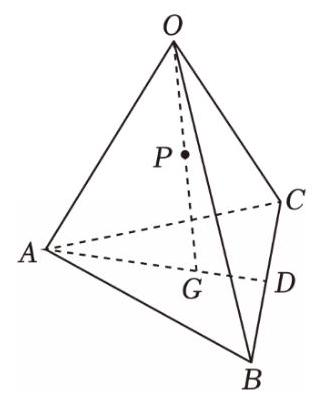
\includegraphics[max width=0.2\textwidth]{images/bo_d6dceus601uc73dvofhg_115_1095_761_312_398_0.jpg}
\end{center}
\hspace*{3em} 

【答案】 \(\frac{1}{6}\overrightarrow{a} + \frac{1}{6}\overrightarrow{b} + \frac{1}{6}\overrightarrow{c}\)

【解析】 \(\overrightarrow{OP} = \frac{1}{2}\overrightarrow{OG} = \frac{1}{2}\left( {\frac{1}{3}\overrightarrow{OA} + \frac{2}{3}\overrightarrow{OD}}\right)  = \frac{1}{2}\left\lbrack  {\frac{1}{3}\overrightarrow{OA} + \frac{1}{3}\left( {\overrightarrow{OB} + \overrightarrow{OC}}\right) }\right\rbrack \; = \frac{1}{6}\overrightarrow{OA} + \frac{1}{6}\overrightarrow{OB} + \frac{1}{6}\overrightarrow{OC} = \frac{1}{6}\overrightarrow{a} + \frac{1}{6}\overrightarrow{b} + \frac{1}{6}\overrightarrow{c} \cdot  \overrightarrow{a} <\)

3.【2025.12 宝山高三一模 12】空间中,向量 \(\overrightarrow{a},\overrightarrow{b},\overrightarrow{c}\) 满足: \(\left| \overrightarrow{a}\right|  = 2\left| \overrightarrow{b}\right|  = 3\left| \overrightarrow{c}\right|  = 6\) ，且 \(\overrightarrow{a},\overrightarrow{b},\overrightarrow{c}\) 的两两夹角都是 \({60}^{ \circ  }\) ,对于向量 \(\overrightarrow{{e}_{1}},\overrightarrow{{e}_{2}}\) ,若 \(\overrightarrow{c} \cdot  \overrightarrow{{e}_{1}} = {12},\left( {\overrightarrow{{e}_{2}} - \overrightarrow{a}}\right) \left( {\overrightarrow{{e}_{2}} - \overrightarrow{b}}\right)  = 0\) ,则 \(\left| {\overrightarrow{{e}_{1}} - \overrightarrow{{e}_{2}}}\right|\) 的最小值是\_\_\_\_\_.

【答案】 \(\frac{{15} - 6\sqrt{3}}{4}\)

【解析】解法一: 由 \(\overrightarrow{c} \cdot  \overrightarrow{{e}_{1}} = {12}\) 可得 \(\left| \overrightarrow{c}\right|  \cdot  \left| \overrightarrow{{e}_{1}}\right| \cos {\theta }_{1} = {12}\) , \(\therefore \left| \overrightarrow{{e}_{1}}\right| \cos {\theta }_{1} = 6\) ,即动向量 \(\overrightarrow{{e}_{1}}\) 在 \(\overrightarrow{c}\) 方向上的数量投影为 6 .

由 \(\left( {\overrightarrow{{e}_{2}} - \overrightarrow{a}}\right) \left( {\overrightarrow{{e}_{2}} - \overrightarrow{b}}\right)  = 0\) ,可设 \(\overrightarrow{d} = \frac{1}{2}\left( {\overrightarrow{a} + \overrightarrow{b}}\right) ,\left| \overrightarrow{d}\right| \cos {\theta }_{2} = \frac{\frac{1}{2}\left( {\overrightarrow{a} + \overrightarrow{b}}\right)  \cdot  \overrightarrow{c}}{\left| \overrightarrow{c}\right| } = \frac{1}{4}\left( {\overrightarrow{a} \cdot  \overrightarrow{c} + \overrightarrow{b} \cdot  \overrightarrow{c}}\right)  = \frac{9}{4}\) , 即向量 \(\overrightarrow{d}\) 在 \(\overrightarrow{c}\) 方向上的数量投影为 \(\frac{9}{4}\) .

\(\therefore {\left| \overrightarrow{d} - \overrightarrow{{e}_{2}}\right| }_{\min } = 6 - \frac{9}{4} = \frac{15}{4}\) ,从而可得 \({\left| \overrightarrow{{e}_{1}} - \overrightarrow{{e}_{2}}\right| }_{\min } = {\left| \overrightarrow{d} - \overrightarrow{{e}_{2}}\right| }_{\min } - \frac{1}{2}\left| {\overrightarrow{a} - \overrightarrow{b}}\right|  = \frac{15}{4} - \frac{3\sqrt{3}}{2} = \frac{{15} - 6\sqrt{3}}{4}\) .

解法二: 为方便书写和画图,设 \(\overrightarrow{a} = \overrightarrow{OA},\overrightarrow{b} = \overrightarrow{OB},\overrightarrow{c} = \overrightarrow{OC},\overrightarrow{{e}_{1}} = \overrightarrow{O{E}_{1}},\overrightarrow{{e}_{2}} = \overrightarrow{O{E}_{2}}\) .

根据 \(\left| \overrightarrow{OA}\right|  = 6,\left| \overrightarrow{OB}\right|  = 3,\angle {AOB} = {60}^{ \circ  }\) 可得 \({BO} \bot  {AB}\) ,于是如图建系,

得 \(O\left( {3,0,0}\right) ,A\left( {0,3\sqrt{3},0}\right)\) . 再由 \(\angle {BOC} = \angle {AOC} = {60}^{ \circ  }\) 可知: 点 \(C\) 在平面 \({AOB}\) 上的投影在 \(\angle {AOB}\) 的角平分线 \({ON}\) 上,其中点 \(N\) 在线段 \({AB}\) 上, \({ON} = 2\sqrt{3}\) .

由三余弦定理可得: \(\cos \angle {CON} \cdot  \cos \angle {AON} = \cos \angle {AOC}\) ，代入计算得 \(\cos \angle {CON} = \frac{\sqrt{3}}{3}\) .

再由 \(\left| \overrightarrow{c}\right|  = 2\) 和 \(\overrightarrow{c} \cdot  \overrightarrow{{e}_{1}} = {12}\) 得 \(\left| \overrightarrow{O{E}_{1}}\right| \cos \left\langle  {\overrightarrow{OC},\overrightarrow{O{E}_{1}}}\right\rangle   = 6\) ，即 \(\left| \overrightarrow{OH}\right|  = 6\) ，此时恰好有

\({HN} \bot\) 平面 \({AOB}\) ,此时 \(H\left( {0,\sqrt{3},2\sqrt{6}}\right) ,\overrightarrow{OH} = \left( {-3,\sqrt{3},2\sqrt{6}}\right)\) .

则可得点 \({E}_{1}\) 的轨迹为平面 \(\alpha\) ,其中 \({OH} \bot\) 平面 \(\alpha\) .

再由 \(\left( {\overrightarrow{{e}_{2}} - \overrightarrow{a}}\right) \left( {\overrightarrow{{e}_{2}} - \overrightarrow{b}}\right)  = 0\) 得 \(\left( {\overrightarrow{O{E}_{2}} - \overrightarrow{OA}}\right) \left( {\overrightarrow{O{E}_{2}} - \overrightarrow{OB}}\right)  = 0\) ,即 \(\overrightarrow{A{E}_{2}} \cdot  \overrightarrow{B{E}_{2}} = 0,\therefore \overrightarrow{A{E}_{2}} \bot  \overrightarrow{B{E}_{2}}\) ,故点 \({E}_{2}\) 的轨迹为以线段 \({AB}\) 为直径的球 \(M\) (点 \(M\) 为线段 \({AB}\) 的中点，

此时 \(M\left( {0,\frac{3}{2}\sqrt{3},0}\right)\) .

\(\left| {\overrightarrow{{e}_{1}} - \overrightarrow{{e}_{2}}}\right|\) 的最小值即为求球 \(M\) 上一动点 \({E}_{2}\) 与平面 \(\alpha\) 上一动点 \({E}_{1}\) 之间的距离 \({E}_{1}{E}_{2}\) 的最小值, 可转化为球心 \(M\) 到平面 \(\alpha\) 的距离 \(M{E}_{1}\) 最小值减去半径 \(\frac{3\sqrt{3}}{2}\) ,

即当 \(M{E}_{1} \bot  \alpha\) 时, \(M{E}_{1}\) 取得最小值.

设 \({E}_{1}\left( {{x}_{0},{y}_{0},{z}_{0}}\right)\) ,可得 \(\overrightarrow{H{E}_{1}} = \left( {{x}_{0},{y}_{0} - \sqrt{3},{z}_{0} - 2\sqrt{6}}\right) ,\overrightarrow{M{E}_{1}} = \left( {{x}_{0},{y}_{0} - \frac{3\sqrt{3}}{2},{z}_{0}}\right)\) .

由 \(\overrightarrow{M{E}_{1}}//\overrightarrow{OH}\) 可设 \(\overrightarrow{M{E}_{1}} = \lambda \overrightarrow{OH}\) ,即 \(\left( {{x}_{0},{y}_{0} - \frac{3\sqrt{3}}{2},{z}_{0}}\right)  = \lambda \left( {-3,\sqrt{3},2\sqrt{6}}\right)\) ,

\(\therefore \left\{  \begin{array}{l} {x}_{0} =  - {3\lambda } \\  {y}_{0} = \sqrt{3}\lambda  + \frac{3\sqrt{3}}{2}\text{ . 再由 }\overrightarrow{H{E}_{1}} \bot  \overrightarrow{OH}\text{ 可得 }\overrightarrow{H{E}_{1}} \cdot  \overrightarrow{OH} =  - 3{x}_{0} + \sqrt{3}\left( {{y}_{0} - \sqrt{3}}\right)  + 2\sqrt{6} \cdot  \left( {{z}_{0} - 2\sqrt{6}}\right)  = 0. \\  {z}_{0} = 2\sqrt{6}\lambda  \end{array}\right.\)

代入计算得 \(\lambda  = \frac{5}{8}\) ,

此时 \(\left| \overrightarrow{M{E}_{1}}\right|  = \frac{5}{8}\left| \overrightarrow{OH}\right|  = \frac{15}{4}\) ，所以 \({\left| \overrightarrow{{E}_{1}{E}_{2}}\right| }_{\min } = \frac{15}{4} - \frac{3\sqrt{3}}{2} = \frac{{15} - 6\sqrt{3}}{4}\) .

\begin{center}
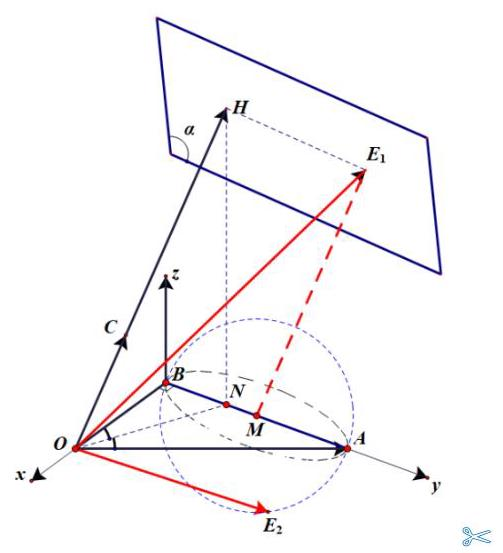
\includegraphics[max width=0.4\textwidth]{images/bo_d6dceus601uc73dvofhg_117_707_206_503_553_0.jpg}
\end{center}
\hspace*{3em} 

\section*{8.4 面积、体积、周长}

1.【2025.12 长宁高三一模 5】圆锥的底面半径为 1 , 母线长为 2 , 则该圆锥的侧面积 2 为\_\_\_\_\_.

【答案】侧面积 \(S = \frac{1}{2}{lR} = \frac{1}{2} \cdot  {2\pi r} \cdot  R = {2\pi } \cdot  3 <\)

2.【2025.12 杨浦高三一模 6】已知圆锥的底面半径为 1，高为 \(\sqrt{3}\) ，则该圆锥的侧面积为\_\_\_\_\_.

【解析】依题意可得: 侧面展开图的半径也即母线长为 2,侧面展开图的弧长为 \(l = {2\pi }\) ,所以侧面积为 \(S = \frac{1}{2} \cdot  {2\pi } \cdot  2 = {2\pi } \cdot  3 <\)

3.【2025.12 闵行高三一模 7】若圆锥的轴截面为等腰直角三角形, 则其侧面展开图扇形圆心角的弧度数为\_\_\_\_\_.

【答案】 \(\sqrt{2}\pi\)

【解析】设底圆半径为 \(r\) ,则母线为 \(R = \sqrt{2}r,\therefore\) 侧面展开图的弧长为 \(l = {2\pi r},\therefore\) 圆心角为 \(\alpha  = \frac{l}{R} = \sqrt{2}\pi\)

4.【2025.12 虹口高三一模 7】已知某圆锥的底面半径为 2，侧面积为 \({6\pi }\) ，则该圆锥的体积为\_\_\_\_\_. (结果保留 \(\pi\)

【答案】 \(\frac{4\sqrt{5}\pi }{3}\)

【解析】依题意可得: 底面周长为 \({4\pi }\) ,即侧面展开图的弧长为 \(l = {4\pi }\) ,所以由 \({S}_{\text{ 扇 }} = \frac{1}{2}{lR}\) 得

母线长为 \(R = 3\) ， \(\therefore\) 圆锥高为 \(h = \sqrt{5}\) ，体积为 \(V = \frac{1}{3}{S}_{\text{ 底 }}h = \frac{4\sqrt{5}\pi }{3}\) . .2

5.【2025.12 黄浦高三一模 7】已知边长为 3 的正 \(\bigtriangleup {ABC}\) 的三个顶点都在球 \(O\) 的球面上,球心 \(O\) 到平面 \({ABC}\) 的距离为 1,则球 \(O\) 的体积为\_\_\_\_\_.

【答案】 \(\frac{32\pi }{3}\)

【解析】依题意可得: 正 \(\bigtriangleup {ABC}\) 的外接圆半径为 \(r = \frac{1}{2} \cdot  \frac{a}{\sin A} = \frac{1}{2} \cdot  \frac{3}{\sin {60}^{ \circ  }} = \sqrt{3}\) .

所以球 \(O\) 的半径为 \(R = \sqrt{{r}^{2} + {d}^{2}} = 2\) ,体积为 \(V = \frac{4}{3}\pi {R}^{3} = \frac{32\pi }{3}\) . 3 .

6.【2025.12 静安高三一模 7】已知圆柱的底面圆的半径与球的半径相等, 若圆柱的表面积与球的表面积也相等，则圆柱的体积 \({V}_{1}\) 与球的体积 \({V}_{2}\) 之比 \({V}_{1} : {V}_{2} =\) \_\_\_\_\_.

【答案】 \(\frac{3}{4}\)

【解析】设圆柱和球的半径均为 \(R\) ,圆柱的高为 \(h\) .

依题意可得: \({{2\pi }{R}^{2} + {2\pi Rh}} = {{4\pi }{R}^{2}}\) ，解得 \(h = R\) ， \(\therefore \frac{{V}_{1}}{{V}_{2}} = \frac{\pi {R}^{2} \cdot  R}{\frac{4}{3}\pi {R}^{3}} = \frac{3}{4}\) .

7.【2025.12 嘉定高三一模 7】已知圆锥侧面展开图中扇形的中心角为 \(\frac{2\pi }{3}\) ，底面周长为 \({2\pi }\) ，则这个圆锥的侧面积为\_\_\_\_\_.

【答案】 \({3\pi }\)

【解析】依题意可得: 母线长为 \(R = \frac{2\pi }{\frac{2\pi }{3}} = 3\) , \(\therefore\) 侧面积为 \(S = \frac{1}{2}{lR} = \frac{1}{2} \cdot  {2\pi } \cdot  3 = {3\pi } \cdot  3 <\)

8.【2025.12 徐汇高三一模 8】一个底面积为 1 的正四棱柱的所有顶点都在同一球面上, 若该球的表面积为 \({4\pi }\) ，则该正四棱柱的高为\_\_\_\_\_.

【答案】 \(\sqrt{2}\)

【解析】设正四棱柱的高为 \(h\) ,其外接球的半径为 \(R\) ,

则 \(\left\{  \begin{array}{l} {\left( \frac{\sqrt{2}}{2}\right) }^{2} + {\left( \frac{h}{2}\right) }^{2} = {R}^{2} \\  {4\pi }{R}^{2} = {4\pi } \end{array}\right.\) ,解得 \(\left\{  {\begin{array}{l} h = \sqrt{2} \\  R = 1 \end{array}. \ll  }\right.\)

9.【2025.12 崇明高三一模 8】已知圆锥的底面半径为 1 , 侧面积为 \({2\pi }\) ,则该圆锥的体积为\_\_\_\_\_.

【答案】 \(\frac{\sqrt{3}\pi }{3}\)

【答案】侧面展开图的弧长也即底面周长为 \(l = {2\pi }\) , \(\therefore\) 母线长 \(R = \frac{2{S}_{\text{ 侧 }}}{l} = 2\) ,

\(\therefore\) 圆锥的高为 \(h = \sqrt{3}\) . 故圆锥的体积为 \(V = \frac{1}{3}{S}_{\text{ 底 }}h = \frac{\sqrt{3}\pi }{3}\) . 3-4

10.【2025.12 浦东高三一模 8】如图，等腰直角 \(\bigtriangleup {APB}\) 的斜边 \({AB}\) 长为 \({2R}\) ，将 \(\bigtriangleup {APB}\) 绕斜边 \({AB}\) 所在直线旋转一周形成的旋转体的体积为\_\_\_\_\_.

\begin{center}
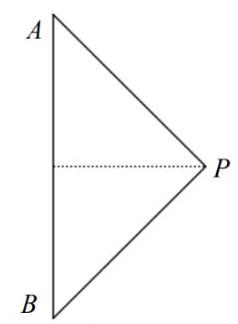
\includegraphics[max width=0.2\textwidth]{images/bo_d6dceus601uc73dvofhg_119_1161_522_238_324_0.jpg}
\end{center}
\hspace*{3em} 

(第 8 题图)

【答案】 \(\frac{2}{3}\pi {R}^{3}\)

【解析】依题意可得: 所得几何体为 2 个大小相同的圆锥,其底面半径为 \(R\) ,高也为 \(R\) . 所以几何体的体积为 \(V = 2 \cdot  \frac{1}{3}\pi {R}^{2} \cdot  R = \frac{2}{3}\pi {R}^{3} \cdot  3 <\)

11.【2025.12 青浦高三一模 9】已知圆柱和圆锥的底面半径相同，侧面积也相等，且它们的高均为 \(\sqrt{2}\) ，则圆锥的体积为\_\_\_\_\_.

【答案】 \(2\sqrt{2}\pi\)

【解析】设底半径均为 \(r\) ,圆锥的母线长 \(R\) ,则二者的侧面积分别为 \({S}_{\text{ 锥 }} = \frac{1}{2} \cdot  {2\pi r} \cdot  R = {\pi Rr}\) , \({S}_{\text{ 柱 }} = {2\pi r} \cdot  \sqrt{2} = 2\sqrt{2}{\pi r}\) ,根据 \({S}_{\text{ 锥 }} = {S}_{\text{ 柱 }}\) 得 \(R = 2\sqrt{2}\) ,

从而可得圆锥的底半径为 \(r = \sqrt{{R}^{2} - {h}^{2}} = \sqrt{6}\) ,所以其体积为 \(V = \frac{1}{3}\pi {r}^{2} \cdot  h = 2\sqrt{2}\pi\) . \(>  <\)

12.【2025.12 松江高三一模 12】在三棱锥 \(P - {ABC}\) 中， \({PA} = 6,{PB} = 8,{PC} = {BC} = 8\sqrt{2}\) ， \(\angle {APB} = {60}^{ \circ  }\) ， \(\angle {APC} = {45}^{ \circ  }\) ，则此三棱锥的体积为\_\_\_\_\_.

【答案】 \({32}\sqrt{3}\)

【解析】延长 \({PA}\) 至 \(D\) ,使得 \({AD} = 2\) ,则 \({PD} = 8\) ,再由 \({PB} = 8,\angle {APB} = {60}^{ \circ  }\) 得 \(\bigtriangleup {PBD}\) 为等边三角形, \({BD} = 8\) . 同时,易得 \({CD} = 8,\therefore {\Delta PCD}\) 和 \(\bigtriangleup {BCD}\) 均为等腰直角三角形,即 \({CD} \bot  {PD}\) , \({CD} \bot  {BD}\) ， \(\therefore {CD} \bot\) 平面 \({PBD}\) .

由等体积法可得 \({V}_{P - {ABC}} = \frac{3}{4}{V}_{C - {PBD}} = \frac{3}{4} \times  \frac{1}{3}{S}_{\bigtriangleup {PBD}} \cdot  {CD} = \frac{3}{4} \times  \frac{1}{3} \times  \left( {\frac{\sqrt{3}}{4} \times  {8}^{2}}\right)  \times  8 = {32}\sqrt{3}\) .

13.【2025.12 金山高三一模 14】已知某正四棱锥的高为 2 ，体积为 24 ，则该正四棱锥的底面边长为 ( )

A. 9 B. 8 C. 6 D. \(2\sqrt{3}\)

【答案】 \(\mathrm{C}\)

【解析】直接套体积公式: \(V = \frac{1}{3}{S}_{\text{ 底 }}h = \frac{1}{3}{a}^{2}h\) ,代入数据计算得 \(a = 6\) ,选 C.

\section*{8.5 大题综合}

\section*{ \circled{1} 线线角}

1.【2025.12 崇明高三一模 18】如图，在直棱柱 \({ABC} - {A}_{1}{B}_{1}{C}_{1}\) 中， \({\angle {BAC}} = {90}^{ \circ  },{AB} = {AC} = \sqrt{2}\) ， \(A{A}_{1} = 3,D\) 是 \({BC}\) 的中点，点 \(E\) 是棱 \(B{B}_{1}\) 上一点.

(1)证明: \({AD}\bot {C}_{1}E\) ；

(2)当异面直线 \({AC},{C}_{1}E\) 所成的角为 \({60}^{ \circ  }\) 时,求三棱锥的 \({B}_{1} - {A}_{1}{C}_{1}E\) 体积.

\begin{center}
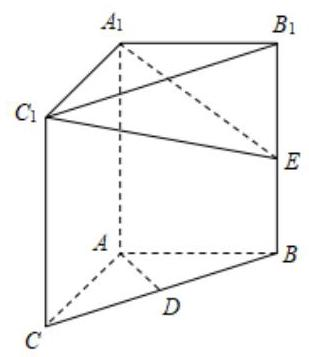
\includegraphics[max width=0.2\textwidth]{images/bo_d6dceus601uc73dvofhg_121_1083_667_309_357_0.jpg}
\end{center}
\hspace*{3em} 

【答案】(1)证明见解析

(2) \(\frac{2}{3}\)

【解析】(1) 证明:因为 \(\mathrm{{AB}} = \mathrm{{AC}},\mathrm{D}\) 是 \(\mathrm{{BC}}\) 的中点,所以 \(\mathrm{{AD}} \bot  \mathrm{{BC}}\) .

又在直三棱柱 \(\mathrm{{ABC}} - {\mathrm{A}}_{1}{\mathrm{\;B}}_{1}{\mathrm{C}}_{1}\) 中, \({\mathrm{{BB}}}_{1} \bot\) 平面 \(\mathrm{{ABC}}\) ,

而 \(\mathrm{{AD}} \subset\) 平面 \(\mathrm{{ABC}}\) ,所以 \(\mathrm{{AD}} \bot  \mathrm{B}{\mathrm{B}}_{1}\) .  \circled{2} 

由 \circled{1}  \circled{2} ,得 \(\mathrm{{AD}}\bot\) 平面 \({\mathrm{{BB}}}_{1}{\mathrm{C}}_{1}\mathrm{C}\) .5 分

因为 \({\mathrm{C}}_{1}\mathrm{E} \subset\) 平面 \({\mathrm{{BB}}}_{1}{\mathrm{C}}_{1}\mathrm{C}\) ,所以 \(\mathrm{{AD}} \bot  {\mathrm{C}}_{1}\mathrm{E}\) .7 分

(2)因为 \(\mathrm{{AC}}\parallel {\mathrm{A}}_{1}{\mathrm{C}}_{1}\) ,所以 \(\angle {\mathrm{A}}_{1}{\mathrm{C}}_{1}\mathrm{E}\) 是异面直线 \(\mathrm{{AC}}\) , \({\mathrm{C}}_{1}\mathrm{E}\) 所成的角(或补角).

由题意知 \(\angle {\mathrm{A}}_{1}{\mathrm{C}}_{1}\mathrm{E} = {60}^{ \circ  }\) . .2 分

因为 \({\mathrm{A}}_{1}{\mathrm{C}}_{1} \bot  {\mathrm{A}}_{1}{\mathrm{\;B}}_{1},{\mathrm{{AA}}}_{1} \bot  {\mathrm{A}}_{1}{\mathrm{C}}_{1}\) ,所以 \({\mathrm{A}}_{1}{\mathrm{C}}_{1} \bot\) 平面 \({\mathrm{A}}_{1}\mathrm{{AB}}{\mathrm{B}}_{1}\) ..4 分

于是 \({\mathrm{A}}_{1}{\mathrm{C}}_{1} \bot  {\mathrm{A}}_{1}\mathrm{E}\) . 故 \({\mathrm{C}}_{1}\mathrm{E} = \frac{{A}_{1}{C}_{1}}{\cos {60}^{ \circ  }} = 2\sqrt{2}\) .

又 \({\mathrm{B}}_{1}{\mathrm{C}}_{1} = \sqrt{{A}_{1}{C}_{1}^{2} + {A}_{1}{B}_{1}^{2}} = 2\) ,所以 \({\mathrm{B}}_{1}\mathrm{E} = \sqrt{{A}_{1}{C}_{1}^{2} + {A}_{1}{B}_{1}^{2}} = 2\) .

从而 \({V}_{\text{ 三棱锥 }{B}_{1} - {A}_{1}{C}_{1}E} = {V}_{\text{ 三棱锥 }{C}_{1} - {A}_{1}{B}_{1}E} = \frac{1}{3}{S}_{\bigtriangleup {A}_{1}{B}_{1}E} \cdot  {\mathrm{A}}_{1}{\mathrm{C}}_{1} = \frac{1}{3} \times  \frac{1}{2} \times  2 \times  \sqrt{2} \times  \sqrt{2} = \frac{2}{3}\) 7 分类

\section*{ \circled{2} 线面角}

1.【2025.12 杨浦高三一模 17】如图，在长方体 \({ABCD} - {A}_{1}{B}_{1}{C}_{1}{D}_{1}\) 中， \(M\) 为 \(B{B}_{1}\) 上一动点， 已知 \({AD} = {CD} = 2,\;{AA}_{1} = 4\) .

(1)求直线 \({A}_{1}C\) 与平面 \({ABCD}\) 所成角的大小；(用反三角表示)

(2)求三棱锥 \(M - A{A}_{1}C\) 的体积.

\begin{center}
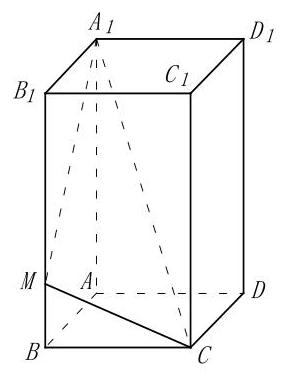
\includegraphics[max width=0.2\textwidth]{images/bo_d6dceus601uc73dvofhg_122_1107_621_281_371_0.jpg}
\end{center}
\hspace*{3em} 

【答案】(1) \(\arctan \sqrt{2}\) (2) \(\frac{8}{3}\)

【解析】(1) 连接 \({AC}\) ,因为 \({A}_{1}A \bot\) 平面 \({ABCD}\) ,

所以 \(\angle {A}_{1}{CA}\) 是直线 \({A}_{1}C\) 与平面 \({ABCD}\) 所成的角,2 分

由 \({AD} = {CD} = 2,\angle {ADC} = {90}^{ \circ  }\) ,所以 \({AC} = 2\sqrt{2}\)

在 Rt \(\Delta {A}_{1}{AC}\) 中, \({AC} = 2\sqrt{2},A{A}_{1} = 4,\angle {A}_{1}{AC} = {90}^{ \circ  },4\) 分

所以 \(\tan \angle {A}_{1}{CA} = \frac{{A}_{1}A}{AC} = \frac{4}{2\sqrt{2}} = \sqrt{2},\angle {A}_{1}{AC} = \arctan \sqrt{2}\)

即直线 \({A}_{1}C\) 与平面 \({ABCD}\) 所成角的大小为 \(\arctan \sqrt{2},6\) 分

( 2 )三棱锥 \(M - A{A}_{1}C\) 的体积 \({V}_{M - {A}_{1}{AC}} = {V}_{C - {MA}{A}_{1}}\) ，8 分

点 \(C\) 到平面 \({MA}{A}_{1}\) 的距离为 \({CB} = {AD} = 2,{10}\) 分

三角形 \({MA}{A}_{1}\) 的面积 \({S}_{{\Delta MA}{A}_{1}} = \frac{1}{2} \cdot  A{A}_{1} \cdot  {BA} = 4,{12}\) 分

所以三棱锥 \(M - A{A}_{1}C\) 的体积 \({V}_{M - {A}_{1}{AC}} = {V}_{C - {MA}{A}_{1}} = \frac{1}{3} \cdot  2 \cdot  4 = \frac{8}{3},{14}\) 分 \(\ll\)

2.【2025.12 青浦高三一模 18】如图,四棱锥 \(P - {ABCD}\) 的底面是边长为 1 的正方形,侧棱 \({PA} \bot\) 底面 \({ABCD}\) ,且 \({PA} = 2\text{ ， }E\) 是侧棱 \({PA}\) 的中点.

(1)求证: \({PC}//\) 平面 \({BDE}\) ；

(2)求证:平面 \({PCD} \bot\) 平面 \({PAD}\) .

\begin{center}
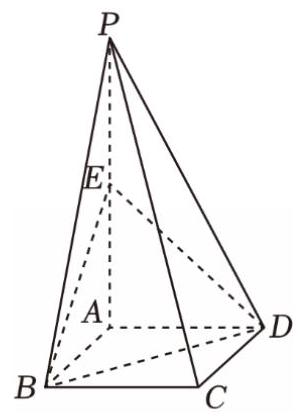
\includegraphics[max width=0.2\textwidth]{images/bo_d6dceus601uc73dvofhg_123_667_465_301_416_0.jpg}
\end{center}
\hspace*{3em} 

\begin{center}
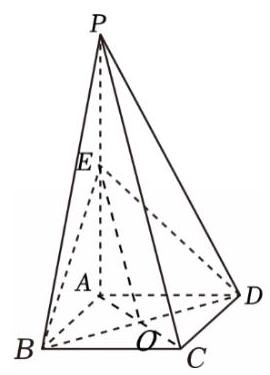
\includegraphics[max width=0.2\textwidth]{images/bo_d6dceus601uc73dvofhg_123_1140_508_270_375_0.jpg}
\end{center}
\hspace*{3em} 

【答案】(1)(2)证明见解析

【解析】(1) 证明: 连接 \({AC}\) 交 \({BD}\) 于 \(O\) ,连接 \({OE}\) ,

因为四边形 \({ABCD}\) 是正方形,所以 \(O\) 是 \({AC}\) 的中点,又 \(E\) 是侧棱 \({PA}\) 的中点,所以 \({PC}//{OE}\) , 又因为 \({OE} \subset\) 平面 \({BDE},{PC} \text{ ⊄ }\) 平面 \({BDE}\) ,所以 \({PC}//\) 平面 \({BDE}\) ;

(2)证明:因为侧棱 \({PA}\bot\) 底面 \({ABCD},{PA} \subset\) 平面 \({PAD}\) ，所以平面 \({PAD}\bot\) 底面 \({ABCD}\) ， 又因为平面 \({PAD} \cap\) 底面 \({ABCD} = {AD},{CD} \subset\) 底面 \({ABCD},{CD} \bot  {AD}\) ,所以 \({CD} \bot\) 平面 \({PAD}\) , 又 \({CD} \subset\) 平面 \({PCD}\) ,所以平面 \({PCD} \bot\) 平面 \({PAD}\) . \(\ll\)

3.【2025.12 嘉定高三一模 18】如图，在四面体 \({VABC}\) 中， \({AC} = {BC}\) ，从顶点 \(V\) 作平面 \({ABC}\) 的垂线,垂足 \(O\) 恰好落在 \(\bigtriangleup  {ABC}\) 的中线 \({CD}\) 上.

(1)如果 \({DV} = {DA} = 2\) ，直线 \({VD}\) 与平面 \({ABC}\) 所成的角为 \(\frac{\pi }{4}\) ，求直线 \({VA}\) 与平面 \({ABC}\) 所成角的大小;

(2)证明:平面 \({VCD} \bot\) 平面 \({VAB}\) .

\begin{center}
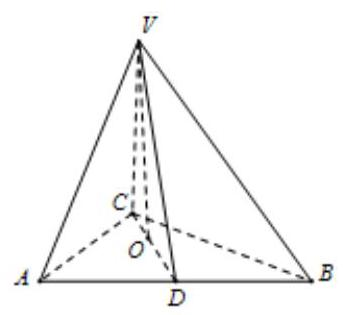
\includegraphics[max width=0.2\textwidth]{images/bo_d6dceus601uc73dvofhg_123_1054_1765_343_315_0.jpg}
\end{center}
\hspace*{3em} 

【答案】(1) \(\frac{\pi }{6}\) (2)证明见解析

【解析】(1) 连接 \({AO}\) .

因为 \({VO} \bot\) 平面 \({ABC}\) ,所以直线 \({VD}\) 与平面 \({ABC}\) 所成的角为 \(\angle {VDO} = \frac{\pi }{4}\) .

在 Rt \(\bigtriangleup {VOD}\) 中, \(\left| {VO}\right|  = \sqrt{2},\left| {DO}\right|  = \sqrt{2}\) .

因为 \({AC} = {BC}\) ， \(D\) 是 \({AB}\) 中点，所以 \({AB}\bot {CD}\) .

在 Rt \(\bigtriangleup {ADO}\) 中,由勾股定理得 \(\left| {AO}\right|  = \sqrt{{\left| AD\right| }^{2} + {\left| DO\right| }^{2}} = \sqrt{6}\) .

因为 \({VO} \bot\) 平面 \({ABC}\) ,所以 \(\angle {VAO}\) 是直线 \({VA}\) 与平面 \({ABC}\) 所成的角.

在 Rt \(\bigtriangleup {VAO}\) 中, \(\tan \angle {VAO} = \frac{\left| VO\right| }{\left| AO\right| } = \frac{\sqrt{2}}{\sqrt{6}} = \frac{1}{\sqrt{3}}\) ,故 \(\angle {VAO} = \frac{\pi }{6}\) 即为所求.

(2)因为 \({VO} \bot\) 平面 \({ABC},{AB} \subset\) 平面 \({ABC}\) ，所以 \({VO} \bot  {AB}\) .

又因为 \({AB} = {AC},D\) 是 \({AB}\) 中点,所以 \({AB} \bot  {CD}\) .

及 \({VO} \cap  {CD} = O\) ,且 \({VO} \subset\) 平面 \({VCD},{CD} \subset\) 平面 \({VCD}\) ,

所以 \({AB} \bot\) 平面 \({VCD}\) . (5 分) \(\ll\)

4.【2025.12 浦东高三一模 18】如图,该几何体由一个棱长为 4 的正方体 \({ABCD} - {A}_{1}{B}_{1}{C}_{1}{D}_{1}\) 与一个半圆柱拼接而成，圆心 \(O\) 、 \({O}_{1}\) 分别为线段 \({AB}\) 、 \({A}_{1}{B}_{1}\) 的中点，动点 \(M\) 在弧 \(\overset{\text{ ⏜ }}{{A}_{1}{B}_{1}}\) 上滑动。

(1)若点 \(M\) 为弧 \(\overset{\text{ ⏜ }}{{A}_{1}{B}_{1}}\) 的中点，求直线 \({MD}\) 与平面 \({BD}{D}_{1}{B}_{1}\) 所成角的大小；

(2)若弧 \(\overset{\text{ ⏜ }}{{A}_{1}M}\) 的长度为 \(\frac{\pi }{2}\) ，求证:平面 \(O{O}_{1}M//\) 平面 \({AC}{C}_{1}{A}_{1}\) .

\begin{center}
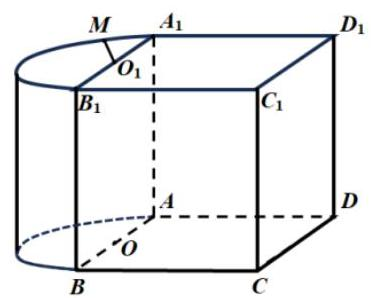
\includegraphics[max width=0.3\textwidth]{images/bo_d6dceus601uc73dvofhg_124_1030_1442_371_298_0.jpg}
\end{center}
\hspace*{3em} 

(第 18 题图)

【答案】(1) \(\arctan \frac{\sqrt{6}}{6}\) (2)证明见解析

【解析】解法一: (1) 连接 \(M{B}_{1},{MD},{B}_{1}D\) .

因为点 \(M\) 为弧 \(\overset{\text{ ⏜ }}{{A}_{1}{B}_{1}}\) 的中点,所以 \(\angle M{B}_{1}{A}_{1} = \frac{\pi }{4}\) , 1 分

故 \(M{B}_{1} \bot  {B}_{1}{D}_{1}\) . 因为 \(B{B}_{1} \bot\) 平面 \({A}_{1}{B}_{1}{C}_{1}{D}_{1}\) ,且 \(M{B}_{1} \subset  {A}_{1}{B}_{1}{C}_{1}{D}_{1}\) ,故 \(M{B}_{1} \bot  B{B}_{1}\) . 由于 \({B}_{1}{D}_{1}\) 和 \(B{B}_{1}\) 是平面 \({BD}{D}_{1}{B}_{1}\) 内的两条相交直线,

所以 \(M{B}_{1} \bot  {BD}{D}_{1}{B}_{1}\) .3 分

因而 \({B}_{1}D\) 是 \({MD}\) 在平面 \({BD}{D}_{1}{B}_{1}\) 上的投影,

所以 \(\angle {MD}{B}_{1}\) 就是直线 \({MD}\) 与平面 \({BD}{D}_{1}{B}_{1}\) 所成的角. .4 分

由题意， \(\left| {M{B}_{1}}\right|  = 2\sqrt{2}\) ， \(\left| {{B}_{1}D}\right|  = 4\sqrt{3}\) ，故 \(\tan \angle {MD}{B}_{1} = \frac{\left| M{B}_{1}\right| }{\left| {B}_{1}D\right| } = \frac{2\sqrt{2}}{4\sqrt{3}} = \frac{\sqrt{6}}{6}\) ，

因此,直线 \({MD}\) 与平面 \(B{B}_{1}{D}_{1}D\) 所成角的大小为 \(\arctan \frac{\sqrt{6}}{6}\) .7 分

(2)由题意， \(\overset{\text{ ⏜ }}{{A}_{1}M} = \frac{\pi }{2},\left| {{A}_{1}{O}_{1}}\right|  = 2\) ，故 \(\angle {A}_{1}{O}_{1}M = \frac{\pi }{4}\) ，

又 \(\angle {O}_{1}{A}_{1}{C}_{1} = \frac{\pi }{4}\) ,所以 \(M{O}_{1}//{A}_{1}{C}_{1}\) .9 分

由 \({A}_{1}{C}_{1} \subset\) 平面 \({AC}{C}_{1}{A}_{1}\) ,且 \(M{O}_{1}\) 不在平面 \({AC}{C}_{1}{A}_{1}\) 内,

可得 \(M{O}_{1}//\) 平面 \({AC}{C}_{1}{A}_{1}\) ; .11 分

同理可得, \(O{O}_{1}//\) 平面 \({AC}{C}_{1}{A}_{1}\) .13 分

又 \(M{O}_{1} \subset\) 平面 \(O{O}_{1}M,O{O}_{1} \subset\) 平面 \(O{O}_{1}M\) ,且 \(M{O}_{1} \cap  O{O}_{1} = {O}_{1}\) ,

所以平面 \(O{O}_{1}M//\) 平面 \({AC}{C}_{1}{A}_{1}\) .14 分

解法二: (1) 由题,点 \(O\text{ 、 }{O}_{1}\) 分别为线段 \({AB}\text{ 、 }{A}_{1}{B}_{1}\) 的中点,故 \(O{O}_{1}//A{A}_{1}\) , 因此 \(O{O}_{1} \bot\) 平面 \({ABCD}\) . 取线段 \({CD}\) 中点 \(G\) ,连接 \({OG}\) ,则 \({OB} \bot  {OG}\) . 标系. 以 \(O\) 为坐标原点,分别以 \(\overrightarrow{OB}\text{ 、 }\overrightarrow{OG}\) 与 \(\overrightarrow{O{O}_{1}}\) 的方向为 \(x\text{ 、 }y\) 与 \(z\) 轴的正方向,建立空间直角坐 1 分

由题意,点 \(M\) 为弧 \(\overset{\text{ ⏜ }}{{A}_{1}{B}_{1}}\) 的中点,故点 \(M\) 的坐标为 \(M\left( {0, - 2,4}\right)\) ,

其他有关点的坐标分别为 \(B\left( {2,0,0}\right) \text{ 、 }D\left( {-2,4,0}\right) \text{ 、 }{D}_{1}\left( {-2,4,4}\right)\) ,

所以 \(\overrightarrow{MD} = \left( {-2,6, - 4}\right) \text{ 、 }\overrightarrow{BD} = \left( {-4,4,0}\right) \text{ 、 }\overrightarrow{D{D}_{1}} = \left( {0,0,4}\right)\) .2 分

设平面 \({BD}{D}_{1}{B}_{1}\) 的法向量为 \(\overrightarrow{n} = \left( {u,v,w}\right)\) ,则 \(\overrightarrow{n} \cdot  \overrightarrow{BD} = 0,\overrightarrow{n} \cdot  \overrightarrow{D{D}_{1}} = 0\) . 即 \(- {4u} + {4v} = 0,{4w} = 0\) .

取 \(u = 1\) ，从而得到平面 \({BD}{D}_{1}{B}_{1}\) 的一个法向量为 \(\overrightarrow{n} = \left( {1,1,0}\right) \ldots {.4}\) 分

设直线 \({MD}\) 与平面 \({BD}{D}_{1}{B}_{1}\) 所成角的大小为 \(\theta \left( {0 \leq  \theta  \leq  \frac{\pi }{2}}\right)\) ,

\(\sin \theta  = \cos \left( {\frac{\pi }{2} - \theta }\right)  = \frac{\left| \overrightarrow{n} \cdot  \overrightarrow{MD}\right| }{\left| \overrightarrow{n}\right|  \cdot  \left| \overrightarrow{MD}\right| } = \frac{4}{\sqrt{56} \cdot  \sqrt{2}} = \frac{\sqrt{7}}{7}.\)

所以直线 \({MD}\) 与平面 \({BD}{D}_{1}{B}_{1}\) 所成角的大小为 \(\arcsin \frac{\sqrt{7}}{7}\) . .7 分

(2)由题意， \(\overset{\text{ ⏜ }}{{A}_{1}M} = \frac{\pi }{2},\left| {{A}_{1}{O}_{1}}\right|  = 2\) ，故 \(\angle {A}_{1}{O}_{1}M = \frac{\pi }{4}\) ，

故点 \(M\) 的坐标为 \(M\left( {-\sqrt{2}, - \sqrt{2},4}\right)\) .9 分

其他相关点的坐标如下: \(O\left( {0,0,0}\right) \text{ 、 }{O}_{1}\left( {0,0,4}\right) \text{ 、 }A\left( {-2,0,0}\right) \text{ 、 }C\left( {2,4,0}\right) \text{ 、 }{C}_{1}\left( {2,4,4}\right)\) ,

所以 \(\overrightarrow{O{O}_{1}} = \left( {0,0,4}\right) \text{ 、 }\overrightarrow{M{O}_{1}} = \left( {\sqrt{2},\sqrt{2},0}\right) \text{ 、 }\overrightarrow{AC} = \left( {4,4,0}\right) \text{ 、 }\overrightarrow{C{C}_{1}} = \left( {0,0,4}\right)\) .

设平面 \(O{O}_{1}M\) 的法向量为 \(\overrightarrow{{n}_{1}} = \left( {{u}_{1},{v}_{1},{w}_{1}}\right)\) ,

由 \(\overrightarrow{{n}_{1}} \cdot  \overrightarrow{O{O}_{1}} = 0,\overrightarrow{{n}_{1}} \cdot  \overrightarrow{M{O}_{1}} = 0\) . 即 \(4{w}_{1} = 0,\sqrt{2}{u}_{1} + \sqrt{2}{v}_{1} = 0\) .

取 \({u}_{1} = 1\) ,得到平面 \(O{O}_{1}M\) 的一个法向量为 \(\overrightarrow{{n}_{1}} = \left( {1, - 1,0}\right) \ldots {11}\) 分

设平面 \({AC}{C}_{1}{A}_{1}\) 的法向量为 \(\overrightarrow{{n}_{2}} = \left( {{u}_{2},{v}_{2},{w}_{2}}\right)\)

由 \(\overrightarrow{{n}_{2}} \cdot  \overrightarrow{AC} = 0,\overrightarrow{{n}_{2}} \cdot  \overrightarrow{C{C}_{1}} = 0\) . 即 \(4{u}_{2} + 4{v}_{2} = 0,4{w}_{2} = 0\) .

取 \({u}_{2} = 1\) ,故平面 \({AC}{C}_{1}{A}_{1}\) 的一个法向量为 \(\overrightarrow{{n}_{2}} = \left( {1, - 1,0}\right)\) 13 分

因为 \({n}_{1}//{n}_{2}\) ,所以平面 \(O{O}_{1}M//\) 平面 \({AC}{C}_{1}{A}_{1}\) .14 分

5.【2025.12 奉贤高三一模 19】如图,将直角三角形 \({SOA}\) 绕直角边 \({SO}\) 所在直线旋转一周形成圆锥 \(S - O\) .

已知圆锥 \(S - O\) 的底面半径为 \(3\mathrm{\;{cm}}\) ,圆锥的侧面积 \({15\pi }{\mathrm{{cm}}}^{2}\) .

设 \(A\text{ 、 }B\) 是底面圆周上的两点,线段 \({AB}\) 不经过点 \(O\) .

(1)求圆锥 \(S - O\) 的体积；

(2)求证:直线 \({SA}\) 与直线 \({OB}\) 是异面直线；

(3)二面角 \(A - {SO} - B\) 的大小为 \(\frac{2\pi }{3}\) ，求直线 \({SA}\) 与平面 \({SOB}\) 所成角的大小.

\begin{center}
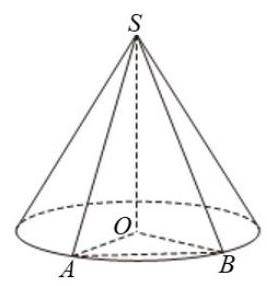
\includegraphics[max width=0.2\textwidth]{images/bo_d6dceus601uc73dvofhg_126_1093_1816_267_286_0.jpg}
\end{center}
\hspace*{3em} 

【答案】(1) \(V = {12\pi c}{m}^{3}\) (2)证明见解析

(3) \(\arcsin \frac{3\sqrt{3}}{10}\)

【解析】(1) \({S}_{\text{ 侧面积 }} = {\pi rl} = {15\pi },\because r = 3,\therefore l = 5.\therefore h = 4,{V}_{\text{ 圆锥 }} = \frac{1}{3}\pi {r}^{2}h = {12\pi }\) .

(2)因为 \(A,O,B\) 三点不共线，所以 \(A,O,B\) 确定唯一一个平面 \({AOB}\)

因为 \(S\) 为圆锥的顶点,所以肯定不在平面 \({AOB}\) 内,

所以直线过平面 \({AOB}\) 外的一点 \(S\) 与平面上一点 \(A\) 的直线 \({SA}\) ,

\({OB}\) 不经过 \(A\) 点，所以 \({SA}\) 与 \({OB}\) 异面.

(3) \(\because {AO} \bot  {SO},{BO} \bot  {SO}\) ，所以 \(\angle {AOB}\) 为二面角的 \(A - {SO} - B\) 的平面角

\(\because {SO} \bot\) 面 \({AOB}\) ,所以面 \({SOB} \bot\) 面 \({AOB}\) 交于 \({OB}\) ,

延长 \({OB}\) ,过 \(A\) 作 \({OB}\) 的延长线的垂线,垂足 \(H\) ,

所以 \({AH} \bot\) 面 \({SOB},\therefore \angle {ASH}\) 为 \({SA}\) 与平面 \({SOB}\) 所成的角,

\({Rt\Delta AHB}\) 中, \(\left| {AH}\right|  = r\sin \left( {\pi  - \frac{2\pi }{3}}\right)  = \frac{3\sqrt{3}}{2},\left| {SA}\right|  = 5\)

\(\sin \angle {ASH} = \frac{\left| AH\right| }{\left| SA\right| } = \frac{3\sqrt{3}}{10}\) ，SA与平面 \({SOB}\) 所成的角大小为 \(\arcsin \frac{3\sqrt{3}}{10} \ll\)

6.【 2025.12 静安高三一模 19】已知正四棱柱 \({ABCD} - {A}_{1}{B}_{1}{C}_{1}{D}_{1}\) 的底面边长为 1,点 \(E\) 、 \(F\) 分别在边 \({AD}\text{ 、 }{CD}\) 上,且 \({AE} = \frac{2}{3},{CF} = \frac{2}{3}\) .

(1)证明: \({AC}//\) 平面 \({B}_{1}{EF}\) ；

(2)若 \({A{A}_{1}} = 2\) ，求直线 \(B{B}_{1}\) 与平面 \({B}_{1}{EF}\) 所成角的正弦值.

\begin{center}
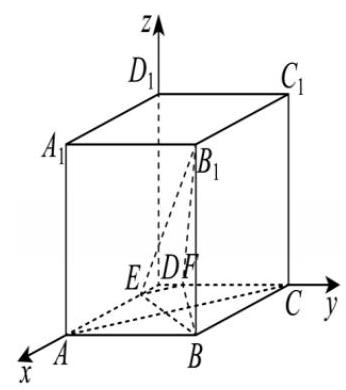
\includegraphics[max width=0.2\textwidth]{images/bo_d6dceus601uc73dvofhg_127_1062_1473_346_390_0.jpg}
\end{center}
\hspace*{3em} 

【答案】(1)证明见解析

(2) \(\frac{5\sqrt{97}}{97}\)

【解析】(1)证明: 因为 \({AE} = \frac{2}{3},{CF} = \frac{2}{3}\) ，所以 \(\frac{ED}{AE} = \frac{DF}{FC} = \frac{1}{2}\) ，

所以 \({AC}//{EF},{AC} \text{ ⊄ }\) 平面 \({B}_{1}{EF},{EF} \subset\) 平面 \({B}_{1}{EF}\) ，所以 \({AC}//\) 平面 \({B}_{1}{EF}\) ；

(2)以 \(D\) 为坐标原点，以 \({DA},{DC},{D{D}_{1}}\) 所在直线分别为 \(x\) 轴， \(y\) 轴， \(z\) 轴建立空间直角坐标别,如图所示: 则 \(B\left( {1,1,0}\right) ,{B}_{1}\left( {1,1,2}\right) ,E\left( {\frac{1}{3},0,0}\right) ,F\left( {0,\frac{1}{3},0}\right)\) ,

则 \(\overrightarrow{B{B}_{1}} = \left( {0,0,2}\right) ,\overrightarrow{E{B}_{1}} = \left( {\frac{2}{3},1,2}\right) ,\overrightarrow{EF} = \left( {-\frac{1}{3},\frac{1}{3},0}\right)\) ,

设平面 \({B}_{1}{EF}\) 的法向量为 \(\overrightarrow{n} = \left( {x,y,z}\right)\) ,则 \(\left\{  \begin{matrix} \overrightarrow{n} \cdot  \overrightarrow{E{B}_{1}} = \frac{2}{3}x + y + {2z} = 0, \\  \overrightarrow{n} \cdot  \overrightarrow{EF} =  - \frac{1}{3}x + \frac{1}{3}y = 0, \end{matrix}\right.\)

取 \(x = 3\) ,则 \(y = 3,z =  - \frac{5}{2}\) ,则平面 \({B}_{1}{EF}\) 的一个法向量为 \(\overrightarrow{n} = \left( {3,3, - \frac{5}{2}}\right)\) ,

设直线 \(B{B}_{1}\) 与平面 \({B}_{1}{EF}\) 所成角为 \(\theta\) ,则 \(\sin \theta  = \frac{\left| \overrightarrow{n} \cdot  \overrightarrow{B{B}_{1}}\right| }{\left| \overrightarrow{n}\right| \left| \overrightarrow{B{B}_{1}}\right| } = \frac{5}{\sqrt{97}}\) ,

所以直线 \(B{B}_{1}\) 与平面 \({B}_{1}{EF}\) 所成角的正弦值是 \(\frac{5\sqrt{97}}{97}\) .

另解: 三棱锥 \({B}_{1} - {BEF}\) 的体积等于三棱锥 \(B - {B}_{1}{EF}\) 的体积.

设点 \(B\) 到平面 \({B}_{1}{EF}\) 的距离为 \(d\) ,则为 \(\frac{1}{3}{S}_{\Delta BEF} \cdot  D{D}_{1} = \frac{1}{3}{S}_{\Delta {B}_{1}{EF}} \cdot  d,{S}_{\Delta BEF} = \frac{5}{18}\)

\(\Delta {B}_{1}{EF}\) 中,易知 \({B}_{1}E = {BF} = \frac{7}{3},{EF} = \frac{\sqrt{2}}{3}\) ,从而 \({S}_{\Delta {B}_{1}{EF}} = \frac{\sqrt{97}}{18}\) ,所以 \(d = \frac{{10}\sqrt{97}}{97}\) ,

设直线 \(B{B}_{1}\) 与平面 \({B}_{1}{EF}\) 所成角为 \(\theta ,\sin \theta  = \frac{d}{B{B}_{1}}\) ,

所以直线 \(B{B}_{1}\) 与平面 \({B}_{1}{EF}\) 所成角的正弦值 \(\frac{5\sqrt{97}}{97}\) . \(\propto\)

 \circled{3} 二面角

1.【2025.12 普陀高三一模 17】如图所示,过圆柱的轴 \(O{O}_{1}\) 的平面与该圆柱相截所形成的截面是边长为 2 的正方形 \(A{A}_{1}{C}_{1}C,B\) 是该圆柱底面圆周上异于 \(A\text{ 、 }C\) 两点的点.

(1)设平面 \({A}_{1}{AB} \cap\) 平面 \({C}_{1}{CB} = l\) ，求证: \(l//A{A}_{1}\) ；

(2)当三棱锥 \({C}_{1} - {ABC}\) 的体积最大时，求二面角 \({C}_{1} - {AB} - C\) 的余弦值.

\begin{center}
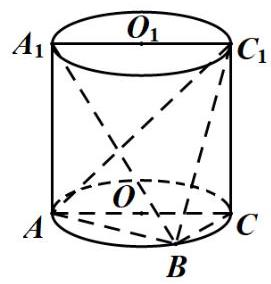
\includegraphics[max width=0.2\textwidth]{images/bo_d6dceus601uc73dvofhg_129_1120_621_271_284_0.jpg}
\end{center}
\hspace*{3em} 

【答案】(1)证明见解析

(2) \(\frac{\sqrt{3}}{3}\)

【解析】(1) 由已知得 \(A{A}_{1}//C{C}_{1}\) ,又 \(C{C}_{1} \subset\) 平面 \({C}_{1}{BC},A{A}_{1}\) 在平面 \({C}_{1}{CB}\) 外,

则 \(A{A}_{1}//\) 平面 \({C}_{1}{CB}\) , .4 分

又平面 \({A}_{1}{AB} \cap\) 平面 \({C}_{1}{CB} = l,A{A}_{1} \subset\) 平面 \({A}_{1}{AB}\) ,则 \(l//A{A}_{1}\) . .6 分

(2)设 \(\bigtriangleup  {ABC}\) 的边 \({AC}\) 上的高为 \(h\) ，则 \({V}_{{C}_{1} - {ABC}} = \frac{1}{3}{S}_{\bigtriangleup {ABC}} \cdot  C{C}_{1} = \frac{2}{3}h\) ，

当三棱锥 \({C}_{1} - {ABC}\) 的体积最大时， \(h = 1\) ，即 \(B\) 为 \(\overset{\text{ ⏜ }}{AC}\) 的中点， .2 分

又 \(C{C}_{1} \bot\) 平面 \({ABC},{CB}\) 是 \({C}_{1}B\) 在平面 \({ABC}\) 上的投影, \({CB} \bot  {AB}\) ,

由三垂线定理得， \({C}_{1}B \bot  {AB}\) ，

则 \(\angle {C}_{1}{BC}\) 是二面角 \({C}_{1} - {AB} - C\) 的平面角, .6 分

在直角三角形 \({CB}{C}_{1}\) 中, \({BC} = \sqrt{2},B{C}_{1} = \sqrt{6}\) ,则 \(\cos \angle {CB}{C}_{1} = \frac{\sqrt{3}}{3}\) ,

即所求的二面角 \({C}_{1} - {AB} - C\) 的余弦值为 \(\frac{\sqrt{3}}{3}\) . .8 分

2.【2025.12 闵行高三一模 17】如图,三棱锥 \(P - {ABC}\) 中，侧面 \({PAC}\) 与底面 \({ABC}\) 都是以 \({AC}\) 为斜边的等腰直角三角形, \(O\) 为 \({AC}\) 中点.

(1)求证: \({AC}\bot {PB}\) ；

(2)若 \({PO}\bot {OB}\) ，求二面角 \(P - {AB} - C\) 的大小.

\begin{center}
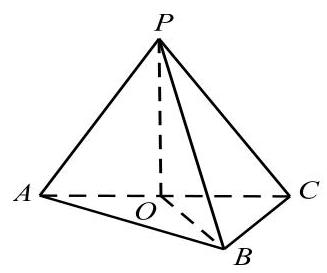
\includegraphics[max width=0.2\textwidth]{images/bo_d6dceus601uc73dvofhg_130_1068_202_327_273_0.jpg}
\end{center}
\hspace*{3em} 

【答案】(1)见解析 (2) \(\arctan \sqrt{2}\)

【解析】(1)因为侧面 \({PAC}\) 与底面 \({ABC}\) 都是以 \({AC}\) 为斜边的等腰直角三角形, \(O\) 为 \({AC}\) 中点. 所以 \({PO} \bot  {AC}\) , \({BO} \bot  {AC},{PO}\) 和 \({BO}\) 是平面 \({PBO}\) 内的两条相交直线,

所以 \({AC} \bot\) 平面 \({PBO}\) ,又 \({PB} \subset\) 平面 \({PBO}\) ,所以 \({AC} \bot  {PB}\) ;

(2)因为 \({PO} \bot  {AC}\) , \({PO} \bot  {OB},{AC}\) 和 \({OB}\) 是平面 \({ABC}\) 两的两条相交直线,

所以 \({PO} \bot\) 平面 \({ABC}\) . 过点 \(O\) 作 \({OH} \bot  {AB}\) ,垂足为 \(H\) ,连结 \({PH}\) ,

因为 \({PH}\) 在面 \({ABC}\) 内的射影为 \({OH}\) ，由三垂线定理得 \({PH} \bot  {AB}\) .

所以二面角 \(P - {AB} - C\) 的平面角为 \(\angle {PHO}\) ,不妨设 \({PO} = {AO} = {OB} = {2a}\) ,则 \({OH} = \sqrt{2}a\) , 所以 \(\tan \angle {PHO} = \frac{\left| PO\right| }{\left| OH\right| } = \sqrt{2}\) ,所以二面角 \(P - {AB} - C\) 的大小为 \(\arctan \sqrt{2} \rightarrow\)

3.【2025.12 金山高三一模 18】如图,已知圆锥 \(A - O\) ,点 \(B\text{ 、 }C\) 在底面圆周上, \({OA} = {OB} = 4\) ， 且 \(\angle {BOC} = {90}^{ \circ  }\) ，动点 \(P\) 落在劣弧 \(\overset{\text{ ⏜ }}{BC}\) 上.

(1)求证:平面 \({AOB} \bot\) 平面 \({AOC}\) ;

(2)若点 \(P\) 平分劣弧 \(\overset{\text{ ⏜ }}{BC}\) ,过点 \(P\) 分别作 \({PD} \bot  {OC}\text{ 、 }{PE} \bot  {OB}\) ,垂足分别为 \(D\text{ 、 }E\) 两点, 求二面角 \(D - {AP} - E\) 的大小.

\begin{center}
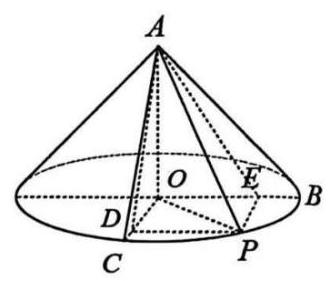
\includegraphics[max width=0.2\textwidth]{images/bo_d6dceus601uc73dvofhg_130_1075_1549_329_281_0.jpg}
\end{center}
\hspace*{3em} 

【答案】(1)证明见解析 (2) \(\pi  - \arccos \frac{1}{3}\)

【解析】(1) 因为 \(\angle {BOC} = {90}^{ \circ  }\) ，所以 \({CO}\bot {BO}\) . 1 分

又因为 \({AO} \bot\) 平面 \({BOC}\) ,且 \({BO} \subset  {BOC}\) ,所以 \({AO} \bot  {CO}\) . .2 分

因为 \({AO} \cap  {BO} = O\) ，且 \({AO} \subset\) 平面 \({AOB}\) ， \({BO} \subset\) 平面 \({AOB}\) ， .3 分

所以 \({CO}\bot\) 平面 \({AOB}\) . .4 分

又因为 \({CO} \subset\) 平面 \({AOC}\) ,所以平面 \({AOB} \bot\) 平面 \({AOC}\) . .6 分

(2)方法一:过点 \(D\) 作 \({DF}\bot {AP}\) ，垂足为 \(F\) ，连接 \({EF}\) ，

由题意得: 四边形 \({OCPE}\) 为正方形. 所以 \(\bigtriangleup {AOD}\) 与 \(\bigtriangleup {AOE}\) 全等.

因为 \({DF} \bot  {AP}\) ,所以 \({EF} \bot  {AP}\) . 所以 \(\angle {DFE}\) 为二面角 \(D - {AP} - E\) 的平面角. .8 分

因为 \({DF} = {EF} = \sqrt{6},{DE} = 4\) , .11 分

所以 \(\cos \angle {DFE} =  - \frac{1}{3}\) . .13 分

所以二面角 \(D - {AP} - E\) 的大小为 \(\pi  - \arccos \frac{1}{3}\) . .14 分

方法二: 以点 \(O\) 为坐标原点,分别以射线 \({OC}\text{ 、 }{OB}\text{ 、 }{OA}\) 为 \(x\) 轴、 \(y\) 轴、 \(z\) 轴的正半轴,建立空间直角坐标系. .7 分

可得: \(A\left( {0,0,4}\right) \text{ 、 }D\left( {2\sqrt{2},0,0}\right) \text{ 、 }E\left( {0,2\sqrt{2},0}\right) \text{ 、 }P\left( {2\sqrt{2},2\sqrt{2},0}\right)\) . .8 分

所以 \(\overrightarrow{DA} = \left( {-2\sqrt{2},0,4}\right) \text{ 、 }\overrightarrow{DP} = \left( {0,2\sqrt{2},0}\right)\) . .9 分

设平面 \({DAP}\) 的法向量为 \(\overrightarrow{{n}_{1}} = \left( {u,v,w}\right)\) ,所以 \(\overrightarrow{{n}_{1}} \bullet  \overrightarrow{DA} = 0,\overrightarrow{{n}_{1}} \bullet  \overrightarrow{DP} = 0\) .

计算得到: \(\left\{  \begin{matrix}  - 2\sqrt{2}u + {4w} = 0 \\  2\sqrt{2}v = 0 \end{matrix}\right.\) , 10 分

取 \(u = \sqrt{2}\) ,从而得到平面 \({DAP}\) 的一个法向量 \(\overrightarrow{{n}_{1}} = \left( {\sqrt{2},0,1}\right)\) . .11 分

同理: 平面 \({EAP}\) 的一个法向量 \(\overrightarrow{{n}_{2}} = \left( {0,\sqrt{2},1}\right)\) . .12 分

所以 \(\cos  < \overrightarrow{{n}_{1}},\overrightarrow{{n}_{2}} >  = \frac{1}{3}\) . .13 分

由图可知,二面角 \(D - {AP} - E\) 为钝角.

所以二面角 \(D - {AP} - E\) 的大小为 \(\pi  - \arccos \frac{1}{3}\) . .14 分

4.【2025.12 黄浦高三一模 18】如图，在几何体 \({ABCDE}\) 中，四边形 \({ABCD}\) 是矩形， \({AB}\) 上平面 \({BEC},{BE} \bot  {EC},{AB} = {BE} = {EC} = 2\) ,

\(G,F\) 分别是线段 \({BE},{DC}\) 的中点.

(1)求证: \({GF}//\) 平面 \({ADE}\) ；

(2)设平面 \({AEF}\) 与平面 \({BEC}\) 的交线为 \(l\) ，求二面角 \(A - l - B\) 的大小.

\begin{center}
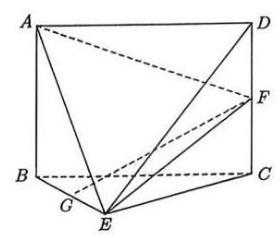
\includegraphics[max width=0.2\textwidth]{images/bo_d6dceus601uc73dvofhg_132_247_598_280_238_0.jpg}
\end{center}
\hspace*{3em} 

\begin{center}
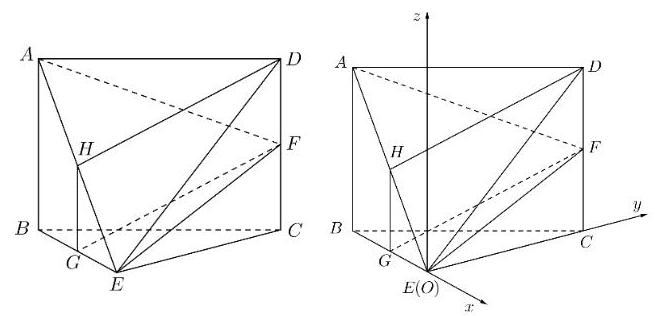
\includegraphics[max width=0.5\textwidth]{images/bo_d6dceus601uc73dvofhg_132_628_556_655_316_0.jpg}
\end{center}
\hspace*{3em} 

【答案】(1)证明见解析

(2) \(\arccos \frac{2}{3}\)

【解析】(1) 设 \(H\) 是 \({AE}\) 的中点,连 \({GH},{HD}\) ,

\(\because G,H\) 分别是 \({BE},{AE}\) 的中点, \(\therefore {GH} = \frac{1}{2}{AB}\) ,

又 \(F\) 是 \({DC}\) 中点,且四边形 \({ABCD}\) 是矩形, \(\therefore {DF} = \frac{1}{2}{AB}\) ,

\(\therefore {GH} =\) \_ \({DF}\) ，故四边形 \({GHDF}\) 是平行四边形，所以 \({HD}\parallel {GF}\) ， .4 分

又 \({HD} \subset\) 平面 \({ADE},{GF} \text{ ⊄ }\) 平面 \({ADE},\therefore {GF}\parallel\) 平面 \({ADE}\) . .6 分

(2)以 \(E\) 为坐标原点， \({BE},{EC}\) 为 \(x,y\) 轴，过 \(E\) 且与平面

\({BEC}\) 垂直的直线为 \(z\) 轴,建立空间直角坐标系 \(O - {xyz}\) ,

由 \({AB} \bot\) 平面 \({EBC}\) ,可得 \({AB}\parallel z\) 轴. .7 分

由 \(E\left( {0,0,0}\right) ,A\left( {-2,0,2}\right) ,F\left( {0,2,1}\right)\) ,得 \(\overrightarrow{EA} = \left( {-2,0,2}\right) ,\overrightarrow{EF} =\)

\(\left( {0,2,1}\right)\) ,设 \(\overrightarrow{n} = \left( {x,y,1}\right)\) 是平面 \({AEF}\) 的一个法向量,二面角 \(A - l - B\) 的大小为 \(\theta\) . 由 \(\left\{  \begin{array}{l} \overrightarrow{n} \cdot  \overrightarrow{EA} =  - {2x} + 2 = 0, \\  \overrightarrow{n} \cdot  \overrightarrow{EF} = {2y} + 1 = 0, \end{array}\right.\) 可得 \(\left\{  \begin{matrix} x = 1, \\  y =  - \frac{1}{2}, \end{matrix}\right.\) 故 \(\overrightarrow{n} = \left( {1, - \frac{1}{2},1}\right)\) . 10 分

又 \(\overrightarrow{BA} = \left( {0,0,2}\right)\) 是平面 \({EBC}\) 的一个法向量,所以 \(\cos \theta  = \frac{\left| \overrightarrow{n} \cdot  \overrightarrow{BA}\right| }{\left| \overrightarrow{n}\right|  \cdot  \left| \overrightarrow{BA}\right| } = \frac{2}{\frac{3}{2} \cdot  2} = \frac{2}{3}\) , .13 分可得 \(\theta  = \arccos \frac{2}{3}\) ,故二面角 \(A - l - B\) 的大小为 \(\arccos \frac{2}{3}\ldots {14}\) 分 \(\leq\)

5.【2025.12 长宁高三一模 19】如图, 在四棱锥 P-ABCD 中, PA⊥平面 ABCD, AB⊥AD, \(\mathrm{{AD}}//\mathrm{{BC}},\mathrm{{AB}} = \mathrm{{BC}} = 1,\mathrm{{AD}} = 2\) ，直线 \(\mathrm{{PC}}\) 与平面 \(\mathrm{{ABCD}}\) 所成的角的大小为 \(\arctan \sqrt{2}\) .

(1)求四棱锥 P-ABCD 的体积;

(2)点Q在线段 PD 上，直线 PB//平面 \(\mathrm{{AQC}}\) ，求二面角 Q-AC-D 的余弦值.

\begin{center}
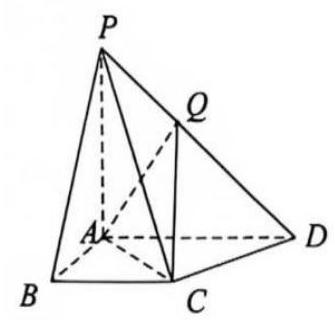
\includegraphics[max width=0.2\textwidth]{images/bo_d6dceus601uc73dvofhg_133_1069_515_335_320_0.jpg}
\end{center}
\hspace*{3em} 

【答案】(1) \(V = \frac{1}{3}{PA} \times  S = 1\) (2) \(\cos \theta  = \frac{\left| \overrightarrow{n} \cdot  \overrightarrow{m}\right| }{\left| \overrightarrow{n}\right| \left| \overrightarrow{m}\right| } = \frac{1}{3}\)

【解析】(1) 因为 \(\mathrm{{PA}} \bot\) 平面 \(\mathrm{{ABCD}}\) ,所以 \(\angle \mathrm{{PCA}}\) 即是直线 \(\mathrm{{PC}}\) 与平面 \(\mathrm{{ABCD}}\) 所成的角.

因为 \({AB} \bot  {AD},{AD}//{BC}\) ,所以 \({AB} \bot  {BC},\) 又 \({AB} = {BC} = 1\) ,所以 \({AC} = \sqrt{2}\) ,

因为 \(\angle {PCA} = \arctan \sqrt{2}\) ,所以 \(\mathrm{{PA}} = 2\) .

梯形 \(\mathrm{{ABCD}}\) 的面积 \(S = \frac{3}{2}\) ，四棱锥 P-ABCD 的体积 \(V = \frac{1}{3}{PA} \times  S = 1\) .

(2)因为 \(\mathrm{{PA}} \bot\) 平面 \(\mathrm{{ABCD}}\) ，所以 \(\mathrm{{PA}} \bot  \mathrm{{AB}}\) ， \(\mathrm{{PA}} \bot  \mathrm{{AD}}\) ，又知 \(\mathrm{{AB}} \bot  \mathrm{{AD}}\) ，

以 \(\mathrm{A}\) 为原点, \(\mathrm{{AB}}\text{ 、 }\mathrm{{AD}}\text{ 、 }\mathrm{{AP}}\) 分别为 \(x\) 轴、 \(y\) 轴、 \(z\) 轴建立空间直角坐标系.

\(A\left( {0,0,0}\right) ,B\left( {1,0,0}\right) ,C\left( {1,1,0}\right) ,D\left( {0,2,0}\right) ,P\left( {0,0,2}\right)\) ,

\(\overrightarrow{AC} = \left( {1,1,0}\right) ,\;\overrightarrow{BP} = \left( {-1,0,2}\right) .\)

设平面 \(\mathrm{{AQC}}\) 的法向量为 \(\overrightarrow{n} = \left( {x,y,z}\right)\) ,则 \(\overrightarrow{n} \cdot  \overrightarrow{AC} = x + y = 0\) ,

因为直线 \(\mathrm{{PB}}//\) 平面 \(\mathrm{{AQC}}\) ,所以 \(\overrightarrow{n}\bot \overrightarrow{BP}\) ,得 \(\overrightarrow{n} \cdot  \overrightarrow{BP} =  - x + {2z} = 0\)

取 \(z = 1\) ,得 \(\overrightarrow{n} = \left( {2, - 2,1}\right)\) ,平面 \(\mathrm{{ABC}}\) 的法向量 \(\overrightarrow{m} = \left( {0,0,1}\right)\) ,

设二面角 \(\mathrm{Q} - \mathrm{{AC}} - \mathrm{D}\) 的大小为 \(\theta\) ，则 \(\cos \theta  = \frac{\left| \overrightarrow{n} \cdot  \overrightarrow{m}\right| }{\left| \overrightarrow{n}\right| \left| \overrightarrow{m}\right| } = \frac{1}{3}\) .

6.【2025.12 徐汇高三一模 19】如图,已知 \({BD}\) 是 \(\odot  O\) 的直径,点 \(C\) 是 \(\odot  O\) 上异于 \(B\text{ 、 }D\) 的一点. 设过点 \(C\) 的直线 \({AC}\) 垂直于 \(\odot  O\) 所在的平面,且 \({AC} = {BD} = 2\) .

(1)若 \(C\) 为 \(\overset{\text{ ⏜ }}{BD}\) 中点， \(E\) 为线段 \({AC}\) 的中点， \(F\) 为线段 \({AD}\) 上一点，且 \({EF}//\) 平面 \({BCD}\) ，求证: \(F\) 为线段 \({AD}\) 中点，并求三棱锥 \(F - {BCD}\) 的体积；

(2)记二面角 \(A - {BD} - C\) 的平面角为 \(\theta\) ，求 \(\theta\) 的最小值，并指出其取得最小值时点 \(C\) 的位置.

\begin{center}
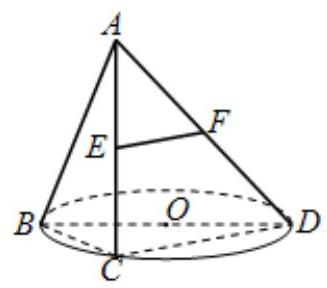
\includegraphics[max width=0.2\textwidth]{images/bo_d6dceus601uc73dvofhg_134_581_616_327_288_0.jpg}
\end{center}
\hspace*{3em} 

\begin{center}
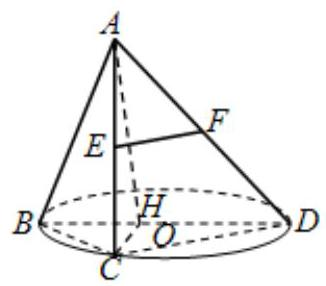
\includegraphics[max width=0.2\textwidth]{images/bo_d6dceus601uc73dvofhg_134_1076_619_326_286_0.jpg}
\end{center}
\hspace*{3em} 

【答案】(1) 证明见解析, \(V = \frac{1}{3}\)

(2)当 \(C\) 为 \(\overset{\text{ ⏜ }}{BD}\) 中点时 \(\theta  = \arctan 2\) ，所以 \(\theta\) 的最小值为 \(\arctan 2\) .

【解析】(1) 由 \({EF}//\) 平面 \({BCD}\text{ 、 }{EF} \subset\) 平面 \({ACD}\) 、平面 \({ACD} \cap\) 平面 \({BCD} = {CD}\) , 结合线面平行的性质定理,有 \({EF}//{CD}\) ,

因为 \(E\) 是 \({AC}\) 中点,所以 \({EF}\) 为 \(\bigtriangleup {ACD}\) 中位线,所以 \(F\) 为 \({AD}\) 中点.

因为 \(C\) 为 \(\overset{\text{ ⏜ }}{BD}\) 中点且直径 \({BD} = 2\) ,所以 \(\angle {BCD} = {90}^{ \circ  }\) ,进而 \({BC} = {BD} = \sqrt{2}\) .

因为过点 \(C\) 得直线 \({AC}\) 垂直于 \(\odot  O\) 所在的平面,

所以 \({AC}\) 是四面体 \(A - {BCD}\) 以 \(\bigtriangleup {BCD}\) 为底面的高,

所以 \({V}_{F - {BCD}} = {V}_{E - {BCD}} = \frac{1}{2}{V}_{A - {BCD}} = \frac{1}{2} \cdot  \frac{1}{3} \cdot  {S}_{\bigtriangleup {BCD}} \cdot  {AC} = \frac{1}{2} \cdot  \frac{1}{3}\left( {\frac{1}{2}\sqrt{2} \cdot  \sqrt{2}}\right) 2 = \frac{1}{3}\) .

(2)如图，作 \({CH}\bot {BD}\) 于 \(H\) ，联结 \({AH}\) .

因为 \({AC} \bot\) 平面 \({BCD}\) ,所以 \({CH}\) 为 \({AH}\) 在平面 \({BCD}\) 上的投影.

由三垂线定理得， \({AH} \bot  {BD}\) . 所以 \(\angle {AHC}\) 即二面角 \(A - {BD} - C\) 的平面角.

因为 \({AC} \bot\) 平面 \({BCD},{CH} \subset\) 平面 \({BCD}\) ,所以 \({AC} \bot  {CH}\) ,

所以 \(\tan \theta  = \frac{AC}{CH} = \frac{2}{CH} \geq  \frac{2}{1} = 2\) . 于是有 \(\theta  \geq  \arctan 2\) ,且当 \(C\) 为 \(\overset{\text{ ⏜ }}{BD}\) 中点时 \(\theta  = \arctan 2\) ,所以 \(\theta\) 的最小值为 \(\arctan 2\) .

\section*{ \circled{4}  点面距}

1.【2025.12 虹口高三一模 17】如图,已知四棱锥 \(P - {ABCD}\) 的底面是边长为 2 的菱形,点 \(E\) 为 \({PC}\) 中点.

(1)若点 \(F\) 是线段 \({BD}\) 上的动点，求证:直线 \({EF}\) 与直线 \({PA}\) 不相交；

(2)若 \({PC} \bot\) 平面 \({ABCD}\) ， \({AC} = {BD}\) ， \({EC} = 1\) ，求点 \(A\) 到平面 \({EBD}\) 的距离.

\begin{center}
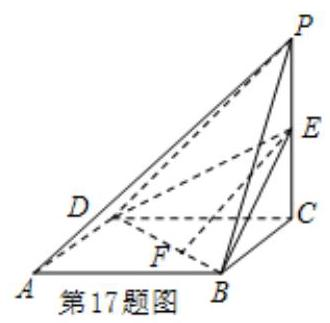
\includegraphics[max width=0.2\textwidth]{images/bo_d6dceus601uc73dvofhg_135_1051_549_330_323_0.jpg}
\end{center}
\hspace*{3em} 

【答案】(1)证明略

(2) \(\frac{\sqrt{6}}{3}\)

【解析】(1) 连接 \({AC}\) ,交 \({BD}\) 于 \(O\) ,连接 \({OE}\) ,则 \({OE}//{PA}\) . 2 分

\({OE} \subset\) 平面 \({EDB}\) ， \({PA}\) 不在平面 \({EDB}\) 上，则 \({PA}//\) 平面 \({EDB}\) . 4 分

所以 \({PA} \cap\) 平面 \({EDB} = \varnothing\) ,且 \({EF} \subset\) 平面 \({EDB}\) ,故直线 \({EF}\) 与直线 \({PA}\) 不相交. 6 分

(2) 由题,可得四边形 \({ABCD}\) 为正方形,所以 \({CD} \bot  {BC}\) . 8 分

以 \(C\) 为原点,以 \(\overrightarrow{CD}\text{ 、 }\overrightarrow{CB}\text{ 、 }\overrightarrow{CP}\) 的方向分别为 \(x\text{ 、 }y\text{ 、 }z\) 的正方向,建立空间直角坐标系,

则 \(\overrightarrow{EB} = \left( {0,2, - 1}\right) \text{ 、 }\overrightarrow{ED} = \left( {2,0, - 1}\right) \text{ 、 }\overrightarrow{AE} = \left( {-2, - 2,1}\right) .{10}\) 分

设 \(\overrightarrow{n} = \left( {x,y,z}\right)\) 为平面 \({EBD}\) 的一个法向量,则 \(\left\{  \begin{array}{l} \overrightarrow{n} \cdot  \overrightarrow{EB} = 0, \\  \overrightarrow{n} \cdot  \overrightarrow{ED} = 0, \end{array}\right.\) 故 \(\left\{  \begin{array}{l} {2y} - z = 0, \\  {2x} - z = 0, \end{array}\right.\)

取 \(x = 1\) ，则 \(\overrightarrow{n} = \left( {1,1,2}\right)\) . 12 分

则 \({d}_{A - {BDE}} = \frac{\left| \overrightarrow{n} \cdot  \overrightarrow{AE}\right| }{\left| \overrightarrow{n}\right| } = \frac{\sqrt{6}}{3} \cdot  {14}\) 分

2.【2025.12 宝山高三一模 17】如图，在四棱锥 \(P - {ABCD}\) 中， \({PD} \bot\) 底面 \({ABCD}\) ，且底面 \({ABCD}\) 为正方形, \(E,F,G\) 分别是 \({BC},{AD},{PA}\) 的中点.

(1)证明: \({PE}//\) 平面 \({BFG}\) ；

(2)若 \({AB} = 2\) ，求点 \(E\) 到平面 \({BFG}\) 的距离.

\begin{center}
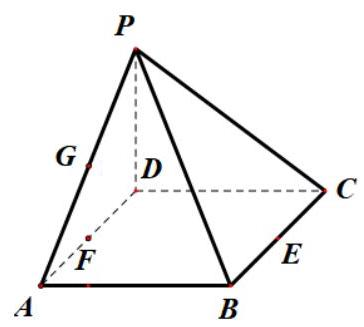
\includegraphics[max width=0.3\textwidth]{images/bo_d6dceus601uc73dvofhg_136_473_496_364_327_0.jpg}
\end{center}
\hspace*{3em} 

\begin{center}
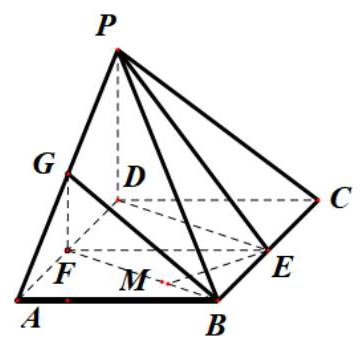
\includegraphics[max width=0.3\textwidth]{images/bo_d6dceus601uc73dvofhg_136_1027_480_360_343_0.jpg}
\end{center}
\hspace*{3em} 

【答案】(1)证明见解析

(2) \(\frac{2\sqrt{5}}{5}\)

【解析】(1) 连接取 \({BF}\) 、 \({AE}\) 交于点 \(T\) ，易知 \({AF} = {BE},{AF}//{BE}\) ，

所以四边形 \({ABEF}\) 为矩形,从而点 \(T\) 平分 \({AE}\) ,

又 \(G\) 是是 \({AP}\) 的中点,所以在 \(\bigtriangleup {APE}\) 中, \({PE}//{GT}\) ,

又因为 \({GT} \subset\) 平面 \({BFG},{PE} \text{ ⊄ }\) 平面 \({BFG}\) 所以 \({PE}//\) 平面 \({BFG}\) .

(2)因为 \({PD} \bot\) 底面 \({ABCD}\) ， \({GF}//{PD}\)

所以 \({GF} \bot\) 底面 \({ABCD}\) ,且 \({GF} = \frac{1}{2}{PD}\)

过点 \(E\) 在平面 \({ABCD}\) 内作 \({EM} \bot  {BF}\) ,垂足为 \(M\) ,则 \({GF} \bot  {EM}\)

因为 \({GF} \cap  {BF} = F\) ,所以 \({EM} \bot\) 平面 \({BFG}\) ,所以点 \(E\) 到平面 \({BFG}\) 的距离即为 \({EM}\)

在 \(\bigtriangleup {BEF}\) 中, \({BE} = 1,{EF} = 2,{BE} \bot  {EF}\) ,从而 \({BF} = \sqrt{5}\)

所以由等面积可得 \({EM} = \frac{2}{\sqrt{5}} = \frac{2}{5}\sqrt{5}\) ,即点 \(E\) 到平面 \({BFG}\) 的距离为 \(\frac{2\sqrt{5}}{5}\) .

(2)也可以用等体积法或向量法解答，相应给分。(《太师

3.【2025.12 松江高三一模 18】已知四棱锥 \(P - {ABCD}\) 的底面 \({ABCD}\) 是直角梯形，

\({AB}//{CD},{AB} = {2CD} = 2,\angle {ABC} = {90}^{ \circ  },{\Delta PBC}\) 是边长为 2 的正三角形，侧面 \({PBC}\bot\) 底面 \({ABCD}\) .

(1)证明: \({PA} \bot  {BD}\) ；

(2)求点 \(D\) 到平面 \({PAB}\) 的距离.

\begin{center}
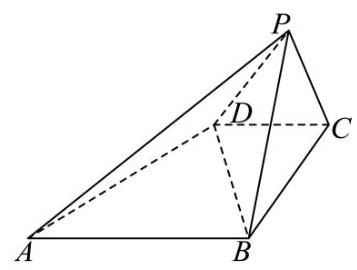
\includegraphics[max width=0.3\textwidth]{images/bo_d6dceus601uc73dvofhg_137_1047_539_357_270_0.jpg}
\end{center}
\hspace*{3em} 

【答案】(1)证明见解析 (2) \(\sqrt{3}\)

【解析】(1) 证明: 取 \({BC}\) 中点 \(\mathrm{H}\) ,连接 \(\mathrm{{AH}},\mathrm{{PH}}\) .

因为 \(\bigtriangleup  {PBC}\) 是正三角形，所以 \({PH}\bot {BC}\) ； 1 分

又因为侧面 \({PBC} \bot\) 底面 \({ABCD}\) ,侧面 \({PBC} \cap\) 底面 \({ABCD} = {BC}\) ,

所以 \({PH} \bot\) 底面 \({ABCD}\) ,所以 \(\mathrm{{PA}}\) 在底面 \({ABCD}\) 上的射影即为 \(\mathrm{{AH}}\) . -3 分在 \(\bigtriangleup {ABH}\) 和 \(\bigtriangleup {BCD}\) 中,

\({BH} = {CD} = 1,{AB} = {BC} = 2,\angle {ABH} = \angle {BCD} = {90}^{ \circ  }\) ,

所以 \(\bigtriangleup {ABH} \cong  \bigtriangleup {BCD}\) ,所以 \(\angle {BAH} = \angle {CBD}\) ,所以 \({AH} \bot  {BD}\) , -5 分所以 \({PA} \bot  {BD}\) . -6 分

(2)因为 \({CD}\parallel {AB}\) ，所以 \(D\) 到平面 \({PAB}\) 的距离即为 \(C\) 到平面 \({PAB}\) 的距离. -7 分因为 \(\angle {ABC} = {90}^{ \circ  }\) ，侧面 \({PBC} \bot\) 底面 \({ABCD}\) ，侧面 \({PBC} \cap\) 底面 \({ABCD} = {BC}\) ，

所以 \({AB} \bot\) 侧面 \({PBC}\) , -9 分

又因为 \({AB} \subset\) 平面 \({PAB}\) ,所以平面 \({PAB} \bot\) 侧面 \({PBC}\) . 10 分

取 \(\mathrm{{PB}}\) 中点 \(\mathrm{E}\) ,连接 \(\mathrm{{CE}}\) ,则 \({CE} \bot  {PB}\) ,所以 \({CE} \bot\) 平面 \({PAB}\) , \(\mathrm{{CE}}\) 即为所求. -12 分因为三角形 \({\Delta PBC}\) 是等边三角形,所以 \({CE} = \sqrt{3}\) .

所以点 \(D\) 到平面 \({PAB}\) 的距离是 \(\sqrt{3}\) . -14 分

\begin{center}
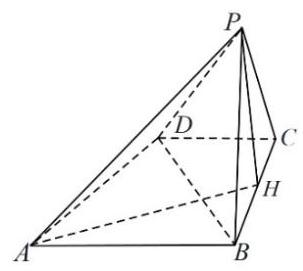
\includegraphics[max width=0.2\textwidth]{images/bo_d6dceus601uc73dvofhg_138_245_239_303_271_0.jpg}
\end{center}
\hspace*{3em} 

\begin{center}
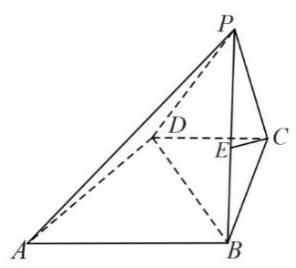
\includegraphics[max width=0.2\textwidth]{images/bo_d6dceus601uc73dvofhg_138_595_240_296_268_0.jpg}
\end{center}
\hspace*{3em} 

\begin{center}
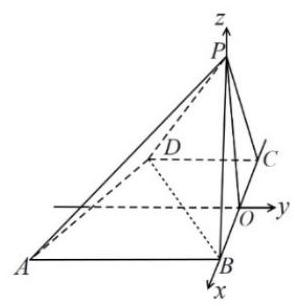
\includegraphics[max width=0.2\textwidth]{images/bo_d6dceus601uc73dvofhg_138_990_219_296_306_0.jpg}
\end{center}
\hspace*{3em} 

\section*{(法二) 建立空间直角坐标系证明:}

(1)取 \({BC}\) 中点 \(O\) ，连接 \({PO}\) . 因为 \({PB} = {PC}\) ，所以 \({PO}\bot {BC}\) ； -1 分又因为侧面 \({PBC} \bot\) 底面 \({ABCD}\) ,侧面 \({PBC} \cap\) 底面 \({ABCD} = {BC}\) ,

所以 \({PO} \bot\) 底面 \({ABCD}\) .

以 \(O\) 为坐标原点, \(\mathrm{{CB}}\) 为 \(x\) 轴, \(\mathrm{{OP}}\) 为 \(z\) 轴,建立如图空间直角坐标系. -3 分

因为 \({AB} = {BC} = 2,{PO} = \sqrt{3}\) ，所以 \(A\left( {1, - 2,0}\right) ,B\left( {1,0,0}\right) ,D\left( {-1, - 1,0}\right) ,P\left( {0,0,\sqrt{3}}\right)\) ，

\(\therefore \overrightarrow{BD} = \left( {-2, - 1,0}\right) ,\overrightarrow{PA} = \left( {1, - 2, - \sqrt{3}}\right)\) ,

\(\because \overrightarrow{BD} \cdot  \overrightarrow{PA} =  - 2 \times  1 + \left( {-1}\right)  \times  \left( {-2}\right)  + 0 \times  \left( {-\sqrt{3}}\right)  = 0\) , 5 分

\(\therefore \overrightarrow{PA} \bot  \overrightarrow{BD},\therefore {PA} \bot  {BD}\) . -6 分

(2)设平面 \({PAB}\) 一个法向量为 \(\overrightarrow{n} = \left( {x,y,z}\right)\) ，因为 \(\overrightarrow{AB} = \left( {0,2,0}\right)\) ， \(\overrightarrow{PB} = \left( {1,0, - \sqrt{3}}\right)\) 所以 \(\left\{  \begin{array}{l} y = 0 \\  x - \sqrt{3}z = 0 \end{array}\right.\) ,不妨设 \(z = 1\) ,则 \(x = \sqrt{3}\) ,所以 \(\overrightarrow{n} = \left( {\sqrt{3},0,1}\right)\) . -10 分

因为 \(\overrightarrow{CB} = \left( {2,0,0}\right)\) ,所以 \(d = \frac{\left| \overrightarrow{CB} \cdot  \overrightarrow{n}\right| }{\left| \overrightarrow{n}\right| } = \frac{2\sqrt{3}}{2} = \sqrt{3}\) . -14 分

本小题也可以用等积法求解.

\section*{第九章 排列组合与二项式}

1、排列数公式: \({P}_{n}^{m} = n\left( {n - 1}\right) \cdots \left( {n - m + 1}\right)  = \frac{n!}{\left( {n - m}\right) !}\left( {n,m \in  {N}^{ * },m \leq  n}\right)\)

2、组合数公式: \({C}_{n}^{m} = \frac{n\left( {n - 1}\right) \cdots \left( {n - m + 1}\right) }{m!} = \frac{n!}{m!\left( {n - m}\right) !}\left( {n \in  {N}^{ * },m \in  N,m \leq  n}\right)\)

3、组合数性质: \({C}_{n}^{m} = {C}_{n}^{n - m};{C}_{n}^{m} + {C}_{n}^{m - 1} = {C}_{n + 1}^{m}\) 。

4、组合数恒等式:

(1) \({C}_{r}^{r} + {C}_{r + 1}^{r} + {C}_{r + 2}^{r} + \cdots  + {C}_{n}^{r} = {C}_{n + 1}^{r + 1}\) ;

(2) \({C}_{n}^{0} + {C}_{n}^{1} + {C}_{n}^{2} + \cdots  + {C}_{n}^{n} = {2}^{n}\) ；

(3) \({C}_{n}^{0} + {C}_{n}^{2} + {C}_{n}^{4} + \cdots  = {2}^{n - 1} = {C}_{n}^{1} + {C}_{n}^{3} + {C}_{n}^{5} + \cdots\) .

(4) \(n{P}_{n - 1}^{k - 1} = {P}_{n}^{k};\frac{n}{m}{C}_{n - 1}^{m - 1} = {C}_{n}^{m}\) .

5、排列数与组合数的关系: \({P}_{n}^{m} = {P}_{n}^{m}{C}_{n}^{m}\)

6、二项式定理 \({\left( a + b\right) }^{n} = {C}_{n}^{0}{a}^{n} + {C}_{n}^{1}{a}^{n - 1}b + \cdots  + {C}_{n}^{r}{a}^{n - r}{b}^{r} + \cdots  + {C}_{n}^{n}{b}^{n}\left( {n \in  {N}^{ * }}\right)\) , 其中通项公式 \({T}_{r + 1} = {C}_{n}^{r}{a}^{n - r}{b}^{r}\) .

7、二项式系数，当 \(\mathrm{n}\) 是偶数时，中间一项 \({C}_{n}^{\frac{n}{2}}\) 取得最大值，当 \(\mathrm{n}\) 是奇数时，中间两项 \({C}_{n}^{\frac{n - 1}{2}} = {C}_{n}^{\frac{n + 1}{2}}\) 取得最大值.

\section*{9.1 排列组合}

1.【2025.12 青浦高三一模 6】现有 5 名学生站成一排, 若学生甲不站两端, 则不同站法共有\_\_\_\_\_种(用数字作答).

【答案】72

【解析】依题意可得: \({C}_{3}^{1}{P}_{4}^{4} = {72}\) 种或 \({P}_{5}^{5} - {C}_{2}^{1}{P}_{4}^{4} = {72}\) 点之

2.【 2025.12 奉贤高三一模 6 】从 3 位女生，4 位男生中选 3 人参加科技比赛，只有 1 位女生入选，则不同的选法有\_\_\_\_\_种\_\_\_\_\_. (用数字表示答案)

【答案】 18

【解析】依题意可得: 共有 \({C}_{3}^{1}{C}_{4}^{2} = {18}\) 种选法.

3.【2025.12 金山高三一模 8】某学校读书节活动中, 甲、乙、丙 3 个班级各有 2 位同学获奖，现将这 6 人排成一排拍照，则同一班级的两位同学均站在一起的排法共有\_\_\_\_\_ 种\_\_\_\_\_

【答案】 48

【解析】依题意有 \({\left( {P}_{2}^{2}\right) }^{3} \cdot  {P}_{3}^{3} = {48}\) 种。

4.【2025.12 虹口高三一模 8】若甲、乙、丙 3 人要站在一个有 7 级台阶的楼梯上拍照，每级台阶至多站 2 人，同一级楼梯上的人不区分站的位置，则不同的站法有\_\_\_\_\_种(结果用数值表示).

【答案】336

【答案】分类讨论:  \circled{1}  \(3 = 2 + 1\) 型,此时有 \({C}_{3}^{2}{P}_{7}^{2} = {126}\) 种;

 \circled{2}  \(3 = 1 + 1 + 1\) 型,此时有 \({P}_{7}^{3} = {210}\) 种.总共有 336 种。

5.【2025.12 徐汇高三一模 9】从 20 名男生和 18 名女生中选取 5 人组成一个宣传小组， 其中男生和女生都不少于 2 人的选法有\_\_\_\_\_种.

【答案】329460

【解析】分 2 种情况:  \circled{1} 3 名男生 2 名女生: \({C}_{20}^{3}{C}_{18}^{2} = {174420}\) 种;

 \circled{2} 2 名男生 3 名女生: \({C}_{20}^{2}{C}_{18}^{3} = {155040}\) . 总共 174420 + 155040 = 329460 种。

6.【2025.12 普陀高三一模 10】某人工智能模型在自然语言处理中，使用位置编码表示词序， 每个位置编码需用一个 6 维向量表示. 若某位置编码可以写成 \(\left( {a,b,c,d,e,f}\right)\) 的形式，其中 \(a\) 、 \(b\text{ 、 }c \in  \{ 1,2,4\}\) ,则在仅考虑前 3 个位置的情况下, \(a\text{ 、 }b\text{ 、 }c\) 恰好取 2 个不同值的编码共有\_\_\_\_\_个.

【答案】 18

【解析】依题意可得: \({C}_{3}^{2}{P}_{3}^{2} = {18}\) 种. \(\approx\)

7.【2025.12 松江高三一模 10】将 3 名男生和 3 名女生排成一排，若从左边第一个学生开始依次往右数，无论数到几人，男生人数都大于或等于女生人数，则有\_\_\_\_\_种不同的排法 (结果用数值表示).

【答案】180

【解析】依题意可得:男 1 号肯定站第一；若男 2 号站第二，则男 3 号可以站第三/四/五这 3 个位置中的任意一个,有 \(3{P}_{3}^{3}{P}_{3}^{3} = {108}\) 种方案; 若男 2 号站第三,则男 3 号可以站第四/ 五这 2 个位置中的任意一个，有 \(2{P}_{3}^{3}{P}_{3}^{3} = {72}\) 种方案. 因此，总共 180 种方案。

8.【2025.12 崇明高三一模 10】7 名学生站成一排拍毕业纪念照, 其中甲必须站在正中间, 并且乙、丙 2 名学生要站在一起，则不同的排法有\_\_\_\_\_种.

【答案】 192

【解析】(不能直接用捆绑法) 分两类: 乙、丙 2 名同时在甲的左侧时, \(2{P}_{2}^{2}{P}_{4}^{4} = {96}\) ;

同理, 乙、丙 2 名同时在甲的右侧时, 也有 96 种排法; 故总共有 192 种方法.

9.【2025.12 闵行高三一模 10】某校的 5 位老师甲、乙、丙、丁、戊排成一排照相, 其中甲、 乙必须相邻，且甲不站在两端，则不同的排法种数为\_\_\_\_\_.

【答案】36

【解析】法 1: 分类讨论:  \circled{1}  甲可以站 2、3、4 号位, 共 3 种选择, 乙对应的均有 2 种选择, 其余 3 人可以任意排列,故总共有 \(3 \times  2 \times  {P}_{3}^{3} = {36}\) 种.

法 2: 先把甲乙捆绑,再减去甲在两端的即可; \({P}_{2}^{2}{P}_{4}^{4} - 2{P}_{3}^{3} = {36} >\)

10.【2025.12 浦东高三一模 11】某城市交通系统采用数智技术记录城市道路口的信号灯状态,每个时段的信号灯状态对应一个数字 (见下表).

\begin{center}
\adjustbox{max width=\textwidth}{
\begin{tabular}{|c|c|c|c|}
\hline
\multirow{2}{*}{信号灯状态} & \multirow{2}{*}{正常绿波协调} & \multicolumn{2}{|c|}{非正常绿波协调} \\
\cline{3-4}
 &  & 道路施工临时黄灯 & 突发事故临时红灯 \\
\cline{1-4}
对应数字 & 0 & 1 & -1 \\
\cline{1-4}
\hline
\end{tabular}
}
\end{center}

(第11题表)

现需要按顺序记录某个道路口 5 个时段的信号灯状态,例如,记号 \(\left( {1,0, - 1,0,1}\right)\) 表示 5 个时段中有 3 个时段是 “非正常绿波协调”状态，分别发生在第1、3、5时段. 问:该路口 5 个时段所有可能的记录中, “非正常绿波协调”的时段数不少于1 个且不多于3 个的记录共有\_\_\_\_\_种。

【答案】 130

【解析】分类讨论: 1 个“非正常绿波协调”有: \({C}_{5}^{1} \cdot  {2}^{1} = {10}\) 种;

2 个“非正常绿波协调”有: \({C}_{5}^{2} \cdot  {2}^{2} = {40}\) 种;

3 个“非正常绿波协调”有: \({C}_{5}^{3} \cdot  {2}^{3} = {80}\) 种;

所以总共有 130 种记录之

11.【2025.12 嘉定高三一模 12】 \({a}_{1}\text{ 、 }{a}_{2}\text{ 、 }{a}_{3}\text{ 、 }{a}_{4}\text{ 、 }{a}_{5}\) 是 \(1\text{ 、 }2\text{ 、 }3\text{ 、 }4\text{ 、 }5\) 的全排列,如果对任意的 \(i \in  \{ 2,3,4\}\) ， \({a}_{i - 1}\) 和 \({a}_{i + 1}\) 中至少有一个大于 \({a}_{i}\) ，则满足要求的排列的总数为\_\_\_\_\_.

【答案】 16

【解析】解法一(分类讨论): 由于 5 是最大的数,因此依题意可得: 5 只能排在 \({a}_{1}\) 或者 \({a}_{5} \cdot\)

当 \({a}_{1} = 1\) 时,此时只可能是 \({a}_{5} = 5\) ,同理 \({a}_{4} = 4,{a}_{3} = 3,{a}_{2} = 2\) ,此时只有 1 种排列方法;

当 \({a}_{2} = 1\) 时, \({a}_{1}\) 有 4 种选择,剩余的 \({a}_{3}\text{ 、 }{a}_{4}\text{ 、 }{a}_{5}\) 只能是 \({a}_{2} < {a}_{3} < {a}_{4} < {a}_{5}\) ,即此时只有 4 种排列方法.

当 \({a}_{3} = 1\) 时, \({a}_{1} > {a}_{2} > 1 < {a}_{4} < {a}_{5}\) ,即此时只有 \({C}_{4}^{2} = 6\) 种排列方法;

对称的情况: 当 \({a}_{4} = 1\) 时,有 4 种排列方法;

当 \({a}_{5} = 1\) 时,只有 1 种排列方法,所以总计 16 种.

解法二(递推归纳):

当 \(n = 3\) 时,有 4 种情况,对应的分别为: \(1,2,3;2,1,3;3,2,1;3,1,2\) (或总共 \({P}_{3}^{3} = 6\) 减去 3 排在中间位置的 2 种情况)；

当 \(n = 4\) 时,最大数字 4 只能排在两端,此时总共 \(4 \times  2 = 8\) 种情况;

当 \(n = 5\) 时,最大数字 5 也是只能排在两端,此时总共 \(4 \times  {2}^{2} = {16}\) 种情况. \(>\)

\section*{9.2 二项式定理}

1.【2025.12 虹口高三一模 3】 \({\left( x - \frac{3}{x}\right) }^{9}\) 的二项展开式中 \({x}^{7}\) 的系数是\_\_\_\_\_.

【答案】 -27

【解析】依题意可得: 通项公式为 \({T}_{r + 1} = {C}_{9}^{r}{x}^{9 - r}{\left( -\frac{3}{x}\right) }^{r} = {C}_{9}^{r}{\left( -3\right) }^{r} \cdot  {x}^{9 - {2r}}\) .

令 \(9 - {2r} = 7\) 得 \(r = 1\) ， \(\therefore {x}^{7}\) 的系数是 \({C}_{9}^{1}{\left( -3\right) }^{1} =  - {27}\) .

2.【 2025.12 奉贤高三一模 3】在二项式 \({\left( x + 1\right) }^{9}\) 的展开式中， \({x}^{5}\) 的系数是\_\_\_\_\_.(用数字表示答案)

【答案】 \({C}_{9}^{4} = {126}\)

【解析】通项公式为 \({T}_{r + 1} = {C}_{9}^{r}{x}^{9 - r}\) ,令 \(9 - r = 5\) 得 \(r = 4,\therefore {x}^{5}\) 的系数是 \({C}_{9}^{4} = {126}\) . \(\approx\)

3.【2025.12 闵行高三一模 4】 \({\left( x + 1\right) }^{5}\) 的二项展开式中 \({x}^{3}\) 项的系数为\_\_\_\_\_.

【答案】 10

【解析】通项公式为 \({T}_{r + 1} = {C}_{5}^{r}{x}^{5 - r}\) ,当 \(5 - r = 3\) 时, \(r = 2,{x}^{3}\) 项的系数为 \({C}_{5}^{2} = {10} \cdot  3 <\)

4.【2025.12 长宁高三一模 4】 \({\left( x - 1\right) }^{6}\) 的展开式中 \({x}^{2}\) 项的系数为\_\_\_\_\_.

【答案】通项公式为 \({T}_{r + 1} = {C}_{6}^{r}{x}^{6 - r}{\left( -1\right) }^{r}\) ,

当 \(6 - r = 2\) 时， \(r = 4,{x}^{2}\) 项的系数为 \({C}_{6}^{4}{\left( -1\right) }^{4} = {15}\) . \(>  <\)

5.【2025.12 青浦高三一模 4】 \({\left( {x}^{3} + \frac{1}{{x}^{2}}\right) }^{5}\) 的二项展开式中的常数项是\_\_\_\_\_(用数字作答).

【答案】 10

【解析】通项公式为 \({T}_{r + 1} = {C}_{5}^{r}{\left( {x}^{3}\right) }^{5 - r}{\left( \frac{1}{{x}^{2}}\right) }^{r} = {C}_{5}^{r} \cdot  {x}^{{15} - {5r}}\) . 令 \({15} - {5r} = 0\) 得 \(r = 3\) , \(\therefore\) 常数项是 \({C}_{5}^{3} = {10} \cdot  3 <\)

6.【2025.12 浦东高三一模 4】求 \({\left( x + \frac{1}{x}\right) }^{6}\) 的二项展开式中的常数项\_\_\_\_\_.

【答案】 20

【解析】通项公式为 \({T}_{r + 1} = {C}_{6}^{r}{x}^{6 - r}{\left( \frac{1}{x}\right) }^{r} = {C}_{6}^{r}{x}^{6 - {2r}}\) ,令 \(6 - {2r} = 0\) 得 \(r = 3\) ,

\(\therefore\) 常数项是 \({C}_{6}^{3} = {20} \cdot  3 <\)

7.【2025.12 金山高三一模 5】已知 \({\left( 1 + 2x\right) }^{5} = {a}_{0} + {a}_{1}x + {a}_{2}{x}^{2} + {a}_{3}{x}^{3} + {a}_{4}{x}^{4} + {a}_{5}{x}^{5}\) ,则 \({a}_{3} =\) \_\_\_\_\_. (用数字作答)

【答案】 80

【解析】通项公式为 \({T}_{r + 1} = {C}_{5}^{r}{\left( 2x\right) }^{r} = {C}_{5}^{r}{2}^{r} \cdot  {x}^{r}\) . 当 \(r = 3\) 时, \({a}_{3} = {C}_{5}^{3}{2}^{3} = {80}\) . \(\approx\)

8.【 2025.12 宝山高三一模 5】 \({\left( x + \frac{2}{x}\right) }^{6}\) 的展开式中 \({x}^{4}\) 的系数为\_\_\_\_\_.

【答案】依题意可得: 通项公式为 \({T}_{r + 1} = {C}_{6}^{r}{x}^{6 - r}{\left( \frac{2}{x}\right) }^{r} = {C}_{6}^{r}{2}^{r} \cdot  {x}^{6 - {2r}}\) .

令 \(6 - {2r} = 4\) 得 \(r = 1\) ， \(\therefore {x}^{4}\) 的系数是 \({C}_{6}^{1}{2}^{1} = {12}\) .

9.【2025.12 杨浦高三一模 5】在二项式 \({\left( x - 2\right) }^{6}\) 的展开式中， \({x}^{2}\) 的系数为\_\_\_\_\_.

【答案】 240

【解析】通项公式为 \({T}_{r + 1} = {C}_{6}^{r}{x}^{6 - r}{\left( -2\right) }^{r}\) ,令 \(6 - r = 2\) 得 \(r = 4,\therefore {x}^{2}\) 的系数是 \({C}_{6}^{4}{\left( -2\right) }^{4} = {240}\) . 10.【2025.12 黄浦高三一模 5】若 \({\left( x + a\right) }^{6}\) 的展开式中 \({x}^{3}\) 的系数为 160,则实数 \(a =\) \_\_\_\_\_.

【答案】 \(a = 2\)

【解析】通项公式为 \({T}_{r + 1} = {C}_{6}^{r}{x}^{6 - r}{a}^{r}\) ,当 \(6 - r = 3\) 得 \(r = 3\) ,

故 \({x}^{3}\) 的系数为 \({C}_{6}^{3}{a}^{3} = {160}\) ,解得 \(a = 2\) .

11.【2025.12 嘉定高三一模 6】在 \({\left( 1 - 2x\right) }^{7}\) 的二项展开式中，各项系数的和是\_\_\_\_\_.

【答案】 -1

【解析】令 \(x = 1\) 得所有系数之和为 \({\left( -1\right) }^{7} =  - 1\) .

12.【2025.12 松江高三一模 6】已知 \({\left( {x}^{2} + \frac{1}{x}\right) }^{n}\) 的二项展开式的各项系数之和为 32,则该二项展开式中 \(x\) 项的系数为\_\_\_\_\_(结果用数值表示).

【答案】 10

【解析】依题意可得: \({2}^{n} = {32}\) ， \(\therefore n = 5\) ，此时通项公式为 \({T}_{r + 1} = {C}_{5}^{r}{\left( {x}^{2}\right) }^{5 - r}{\left( \frac{1}{x}\right) }^{r} = {C}_{5}^{r}{x}^{{10} - {3r}}\) . 当 \({10} - {3r} = 1\) 时,得 \(r = 3,\therefore x\) 项的系数为 \({C}_{5}^{3} = {10}\) . \(\approx\)

13.【2025.12 普陀高三一模 6】 \(\left( {1 - \frac{x}{y}}\right) {\left( x + 2y\right) }^{7}\) 的展开式中含 \({x}^{4}{y}^{3}\) 项的系数是\_\_\_\_\_.

【答案】-280

【解析】 \({\left( x + 2y\right) }^{7}\) 的展开式中通项公式为 \({T}_{r + 1} = {C}_{7}^{r}{x}^{7 - r}{\left( 2y\right) }^{r} = {C}_{7}^{r}{2}^{r} \cdot  {x}^{7 - r}{y}^{r}\) .

当 \(r = 3\) 时, \({C}_{7}^{3}{2}^{3} = {280}\) ; 当 \(r = 4\) 时, \({C}_{7}^{4}{2}^{4} = {560}\) ,

\(\therefore {x}^{4}{y}^{3}\) 项的系数为 \({280} - {560} =  - {280},3 <\)

14.【2025.12 崇明高三一模 7】在 \({\left( {x}^{2} + \frac{2}{x}\right) }^{6}\) 的二项展开式中,常数项的值为\_\_\_\_\_.

【答案】 240

【解析】通项公式为 \({T}_{r + 1} = {C}_{6}^{r}{\left( {x}^{2}\right) }^{6 - r}{\left( \frac{2}{x}\right) }^{r} = {C}_{6}^{r}{2}^{r} \cdot  {x}^{{12} - {3r}}\) ,

令 \({12} - {3r} = 0\) 得 \(r = 4\) ， \(\therefore\) 常数项是 \({C}_{6}^{4}{2}^{4} = {240}\) . \(\approx\)

15.【2025.12 徐汇高三一模 7】已知 \({\left( 1 + 2x\right) }^{10} = {a}_{0} + {a}_{1}x + {a}_{2}{x}^{2} + \cdots  + {a}_{10}{x}^{10}\) ,则 \({a}_{3} =\) \_\_\_\_\_.

【答案】依题意可得: 通项公式为 \({T}_{r + 1} = {C}_{10}^{r}{\left( 2x\right) }^{r} = {C}_{10}^{r}{2}^{r} \cdot  {x}^{r}\) .

当 \(r = 3,\therefore {a}_{3} = {C}_{10}^{3}{2}^{3} = {960}\) .

16.【2025.12 徐汇高三一模 16】已知 \(n \in  \mathbb{N}\) ，集合

\({P}_{n} = \left\{  {\overrightarrow{x}\left| {\;\overrightarrow{x} = \left( {{x}_{1},{x}_{2},{x}_{3},\cdots ,{x}_{n}}\right) }\right. ,{x}_{i} \in  \{ 0,1\} ,1 \leq  i \leq  n,i \in  \mathbb{N}}\right\}  \left( \overrightarrow{x}\right)\) 为 \(n\) 维向量) . 若

\(\overrightarrow{a} = \left( {{a}_{1},{a}_{2},{a}_{3},\cdots ,{a}_{n}}\right)  \in  {P}_{n}\) ,其中 \({a}_{i} = 1\left( {1 \leq  i \leq  n,i \in  \mathbb{N}}\right) ,\;\overrightarrow{b} = \left( {{b}_{1},{b}_{2},{b}_{3},\cdots ,{b}_{n}}\right)  \in  {P}_{n}\) .

定义 \(\overrightarrow{a} \cdot  \overrightarrow{b} = \mathop{\sum }\limits_{{i = 1}}^{n}{a}_{i}{b}_{i}\) ,设满足 \(\overrightarrow{a} \cdot  \overrightarrow{b} = m\) 的 \(\overrightarrow{b}\) 的个数为 \(f\left( m\right)\) . 关于下列两个命题的判断,说法正确的是( ).

 \circled{1}  当 \(n = 3\) 时，则 \(\mathop{\sum }\limits_{{m = 0}}^{3}f\left( m\right)  = 8\) ； \circled{2}  当 \(n = {2k}\) ， \(k\) 是正整数时，则 \(\mathop{\sum }\limits_{{m = 0}}^{{n - 1}}f\left( m\right)  = {2}^{n - 1}\) .

A.  \circled{1} 和 \circled{2} 均为真命题 B.  \circled{1} 和 \circled{2} 均为假命题

C.  \circled{1} 为真命题， \circled{2} 为假命题 D.  \circled{1} 为假命题， \circled{2} 为真命题

【答案】C

【解析】依题意可得: \(\overrightarrow{a} \cdot  \overrightarrow{b} = m\) 时, \(f\left( m\right)  = {C}_{n}^{m}\) ;

对命题 \circled{1} :当 \(n = 3\) 时， \(\mathop{\sum }\limits_{{m = 0}}^{3}f\left( m\right)  = {C}_{3}^{0} + {C}_{3}^{1} + {C}_{3}^{2} + {C}_{3}^{3} = {2}^{3} = 8\) ， \circled{1} 为真命题；

对命题 \circled{2} : \(\mathop{\sum }\limits_{{m = 0}}^{{n - 1}}f\left( m\right)  = {C}_{n}^{0} + {C}_{n}^{1} + {C}_{n}^{2} + \cdots  + {C}_{n}^{n - 1} = {2}^{n} - {C}_{n}^{n} = {2}^{n} - 1\) ， ∴ \circled{2} 为假命题:

\section*{第十章 概率统计}

\section*{【知识梳理】}

1. 记必然事件为 \(\Omega\) ,不可能事件为 \(\Phi\) ,随机事件为 \(\mathrm{A}\)

\(P\left( \Omega \right)  = \_ 1\_ ;P\left( \Phi \right)  = \_ 0\_ ;P\left( A\right)  \in  \_ \left\lbrack  {0,1}\right\rbrack\) \_\_\_\_\_

设 \(\mathrm{E}\text{ 、 }\mathrm{\;F}\) 是两个随机事件(填写独立、对立、互斥)

(1)满足 \(E \cup  F = \Omega\) 且 \(E \cap  F = \Phi\) 的 \(\mathrm{E}\) 和 \(\mathrm{F}\) 叫做对立事件;

(2)E、F 不可能同时出现，则 E 和 F 叫做互斥事件；此时 \(P\left( {E \cup  F}\right)  = P\left( E\right)  + P\left( F\right)\)

(3)E、F 互相之间没有影响，则 E 和 F 是互相独立事件；此时 \(P\left( {EF}\right)  = P\left( E\right) P\left( F\right)\)

2.概率加法公式: \(P\left( {A \cup  B}\right)  = P\left( A\right)  + P\left( B\right)  - P\left( {AB}\right)\) 。

3. 设总体有 \(\mathrm{N}\) 个个体,它们分别是 \({x}_{1},{x}_{2},{x}_{3},\cdots {x}_{N}\) ,且它们的平均数为 \(\mu\)

则总体方差 \({\sigma }^{2} = \frac{1}{N}\left\lbrack  {{\left( {x}_{1} - \mu \right) }^{2} + {\left( {x}_{2} - \mu \right) }^{2} + \cdots  + {\left( {x}_{n} - \mu \right) }^{2}}\right\rbrack\)

\(\sigma\) 叫做总体标准差,反映总体中各个个体之间的差别的大小。

4.抽样方法:

(1)随机抽样:抽样过程中能使总体中的每一个个体都有同样的可能性被选入样本。(抽签、利用随机数抽样等)

(2)系统抽样:把总体的每一个个体编号，按某种相等的间隔抽取样本的方法。

(3)分层抽样:把总体分成若干个部分，然后再每个部分进行随机抽样的方法。

将总体个数 \(\mathrm{N}\) 分成 \(\mathrm{k}\) 层,每层的个体数分别记作 \({N}_{1},{N}_{2},{N}_{3},\cdots {N}_{k}\) ,

在每层中分别随机抽取 \({n}_{1},{n}_{2},{n}_{3},\cdots {n}_{k}\) 个个体组成容量为 \(n\) 的样本。

\(\frac{{n}_{1}}{{N}_{1}} = \frac{{n}_{2}}{{N}_{2}} = \frac{{n}_{3}}{{N}_{3}} = \cdots  = \frac{{n}_{k}}{{N}_{k}} = \frac{n}{N}\)

5. 样本为 \({x}_{1},{x}_{2},{x}_{3},\cdots {x}_{n}\) ,样本容量为 \(n\) ,

则总体均值的点估计值为 \(\bar{x} = \frac{{x}_{1} + {x}_{2} + {x}_{3} + \cdots  + {x}_{n}}{n}\)

总体标准差的点估计值为 \(s = \sqrt{\frac{1}{n - 1}\left\lbrack  {{\left( {x}_{1} - \bar{x}\right) }^{2} + {\left( {x}_{2} - \bar{x}\right) }^{2} + \cdots  + {\left( {x}_{n} - \bar{x}\right) }^{2}}\right\rbrack  }\)

6. 取离散值的随机变量叫做离散型随机变量, 其取值概率可用下表给出

\begin{center}
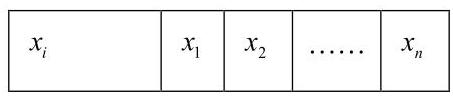
\includegraphics[max width=0.3\textwidth]{images/bo_d6dceus601uc73dvofhg_146_598_2003_453_98_0.jpg}
\end{center}
\hspace*{3em} 

\begin{center}
\adjustbox{max width=\textwidth}{
\begin{tabular}{|c|c|c|c|c|}
\hline
\(P\left( {\xi  = {x}_{k}}\right)\) & \({p}_{1}\) & \({p}_{2}\) & ...... & \({p}_{n}\) \\
\cline{1-5}
\hline
\end{tabular}
}
\end{center}

随机变量所有的取值 \({x}_{1},{x}_{2},\cdots ,{x}_{n}\) 对应的概率所成的数列 \({p}_{1},{p}_{2},\cdots ,{p}_{n}\) 叫做随机变量的概率分布律。

随机变量 \(\xi\) 的数学期望为 \({E\xi } = {x}_{1}{p}_{1} + {x}_{2}{p}_{2} + \cdots  + {x}_{n}{p}_{n}\)

随机变量 \(\xi\) 的方差 \({D\xi } = {\left( {x}_{1} - E\xi \right) }^{2}{p}_{1} + {\left( {x}_{2} - E\xi \right) }^{2}{p}_{2} + \cdots  + {\left( {x}_{n} - E\xi \right) }^{2}{p}_{n}\)

数学期望是随机变量的加权平均数, 表示随机变量取值的平均水平, 因此也叫做随机变量的均值; 随机变量的方差或标准差刻画了随机变量取值的离散程度。

\section*{10.1 概率}

1.【2025.12 虹口高三一模 5】若事件 \(A,B\) 互斥,且 \(P\left( A\right)  = {0.4},P\left( {A \cup  B}\right)  = {0.6}\) ,则 \(P\left( B\right)  =\) \_\_\_\_\_.

【答案】0.2

【解析】依题意可得: \(P\left( {A \cup  B}\right)  = P\left( A\right)  + P\left( B\right) ,\therefore P\left( B\right)  = P\left( {A \cup  B}\right)  - P\left( A\right)  = {0.2}\) .

2.【2025.12 黄浦高三一模 6】甲、乙两人独立破译某个密码，甲译出密码的概率为 0.3 , 乙译出密码的概率为 0.4 ，则该密码被破译的概率为\_\_\_\_\_.

【答案】0.58

【解析】依题意可得: 至少有一人破译该密码的概率为 \(P = 1 - \left( {1 - {0.3}}\right) \left( {1 - {0.4}}\right)  = {0.58}\) . \(\approx\)

3.【2025.12 普陀高三一模 7】设 \(m \in  \mathbf{R}\) ，同时抛掷两枚质地均匀的骰子一次，事件 \(A\) 表示 “第一枚骰子向上的点数为奇数”,事件 \(B\) 表示“两枚骰子向上的点数之和为 \(m\) ”,若事件 \(A\) 与事件 \(B\) 相互独立，则 \(m\) 的一个可取值为\_\_\_\_\_.

【答案】 7

【解析】 \(m = 7\) 时, \(P\left( A\right)  = \frac{1}{2},P\left( B\right)  = \frac{1}{6},P\left( {A \cap  B}\right)  = \frac{3}{36} = \frac{1}{12} = P\left( A\right)  \cdot  P\left( B\right)\) ,满足题意. \(\ll\)

4.【2025.12 嘉定高三一模 8】两个篮球运动员甲和乙罚球时命中的概率分别是 0.7 和 0.6 , 两人各罚球一次，假设事件“甲命中”与“乙命中”是独立的，则至少一人命中的概率是\_\_\_\_\_.

【答案】0.88

【解析】依题意可得: 两人均未命中的概率是 \(P = \left\lbrack  {1 - P\left( A\right) }\right\rbrack  \left\lbrack  {1 - P\left( B\right) }\right\rbrack   = {0.3} \cdot  {0.4} = {0.12}\) , 所以至少一人命中的概率是 \(P = 1 - {0.12} = {0.88}\) .

5.【2025.12 杨浦高三一模 8】已知甲、乙两个篮球运动员罚球的命中率分别为 \(\frac{2}{3},\frac{3}{4}\) ，两人各投一次, 假设事件 “甲命中 ” 与 “乙命中 “是独立的, 则至少有一个人命中的概率为\_\_\_\_\_.

【解析】依题意可得: 两人均未命中的概率是 \(P = \left\lbrack  {1 - P\left( A\right) }\right\rbrack  \left\lbrack  {1 - P\left( B\right) }\right\rbrack   = \frac{1}{3} \times  \frac{1}{4} = \frac{1}{12}\) , 所以至少一人命中的概率是 \(P = 1 - \frac{1}{12} = \frac{11}{12}{.8} <\)

6.【2025.12 宝山高三一模 10】已知事件 \(A\) 与事件 \(B\) 互斥,它们都不发生的概率为 \(\frac{3}{4}\) ,且 \(P\left( A\right)  = {2P}\left( B\right)\) ，则 \(P\left( \bar{A}\right)  =\) \_\_\_\_\_.

【答案】依题意可得: \(P\left( A\right)  + P\left( B\right)  = 1 - \frac{3}{4} = \frac{1}{4}\) ，又 \(\because P\left( A\right)  = {2P}\left( B\right)\) ， \(\therefore \left\{  \begin{array}{l} P\left( A\right)  = \frac{1}{6} \\  P\left( B\right)  = \frac{1}{12} \end{array}\right.\) ， \(\therefore \; P\left( \bar{A}\right)  = \frac{5}{6}.\)

7.【2025.12 崇明高三一模 13】已知事件 \(A\text{ 、 }B\) 相互独立,事件 \(A\) 发生的概率为 \(P\left( A\right)  = \frac{1}{2}\) , 事件 \(B\) 发生的概率为 \(P\left( B\right)  = \frac{1}{2}\) ,则事件 \(A \cap  B\) 发生的概率 \(P\left( {A \cap  B}\right)\) 为( )

A. \(\frac{1}{8}\) B. \(\frac{1}{4}\) C. \(\frac{1}{2}\) D. 0

【答案】B

【解析】依题意可得: \(P\left( {A \cap  B}\right)  = P\left( A\right)  \cdot  P\left( B\right)  = \frac{1}{4}\) ,选 B. \(\leq\)

8.【2025.12 长宁高三一模 14】甲、乙两人投篮的命中率分别为 0.7 和 0.6 ，两人各投篮一次，事件 \(A\) 为甲投中，事件 \(B\) 为乙投中. “甲、乙两人均投中的概率为 0.42 ”是 “事件 \(A,B\) 互相独立”的( ).

A. 充分不必要条件; B. 必要不充分条件;

C. 充要条件; D. 既不充分也不必要条件.

【答案】C. \(\ll\)

9.【2025.12 青浦高三一模 14】抛掷一枚质地均匀的骰子一次，设“出现的点数为偶数”为事件 \(A\) ，“出现的点数大于 4 ”为事件 \(B\) ，则下列描述正确的是( ).

A. 事件 \(A\) 与事件 \(B\) 是对立事件 B. 事件 \(A\) 与事件 \(B\) 是互斥事件

C. 事件 \(A\) 与事件 \(B\) 相互独立 D. \(P\left( {A \cup  B}\right)  = P\left( A\right)  + P\left( B\right)\)

【答案】C

【答案】显然事件 \(A\) 与事件 \(B\) 可以同时发生,如出现点数为 \(6,\therefore\) 它们不是互斥事件, \(\mathrm{B}\) 错误;

事件 \(A\) 与事件 \(B\) 也可可能均不发生,如出现点数为 \(1,\therefore\) 它们不是对立事件, \(\mathrm{A}\) 错误;

事件 \(A\) 包含 3 个基本事件: \(\{ 2,4,6\}\) ,概率为 \(P\left( A\right)  = \frac{1}{2}\) ; 事件 \(B\) 包含 2 个基本事件: \(\{ 5,6\}\) ,

概率为 \(P\left( B\right)  = \frac{1}{3}\) ; 事件 \(A \cap  B\) 包含 1 个基本事件: \(\{ 6\}\) ,概率为 \(P\left( {A \cap  B}\right)  = \frac{1}{6}\) .

\(\because P\left( {A \cap  B}\right)  = P\left( A\right)  \cdot  P\left( B\right)\) , \(\therefore\) 事件 \(A\) 与事件 \(B\) 相互独立, \(\mathrm{C}\) 正确;

事件 \(A \cup  B\) 包含 4 个基本事件: \(\{ 2,4,5,6\}\) ,概率为 \(P\left( {A \cup  B}\right)  = \frac{2}{3}\) ,

此时 \(P\left( {A \cup  B}\right)  \neq  P\left( A\right)  + P\left( B\right)\) , D 错误. \(\ll\)

10.【2025.12 长宁高三一模 17】小明有自觉体锻的习惯，某运动软件记录了其每天运动的时长 (单位:min)，小明从最近 90 天的记录中随机选取了 10 天的记录，具体数据如下: 68、34、70、45、74、126、108、66、36、72.

(1)求这组数据的第 60 百分位数；

(2)运动时长不超过 60min 为不达标，估算从 90 天记录中随机抽取 1 天，该天运动时长不达标的概率;

(3)从这 10 个数中随机删除 2 个数得到一组新的数据，求前后两组数据的极差相同的概率.

【答案】(1)71 (2)0.3

(3) 25

【解析】(1) 将 10 个数按由小到大排列:

34、36、45、66、68、70、72、74、108、126.

\({10} \times  {60}\%  = 6\) ,第 6 个数为 70,第 7 个数为 72,所以第 60 百分位为 71 .

(2)从 10 个数据有 3 个不超过 60 分钟，从 10 个数中选一个，其不达标的概率为 0.3 ， 所以估计从 90 天记录中随机抽取 1 天，该天运动时长不达标的概率为 0.3 .

(3)这组数据的最大值为 126，最小值为 34，

因为删除后极差不变，所以删除的 2 个数不能是 126 和 34,

从 10 个数据中随机删除 2 个数据共有 \({C}_{10}^{2} = {45}\) 种情况

其中使得两组数据极差相同的有 \({C}_{8}^{2} = {28}\) 种情况, 所以前后两组数据的极差相同的概率为 \(\frac{28}{45}\) .

11.【2025.12 静安高三一模 17】为开展社区与学校教育共建活动,某地区教育系统从 \(A\text{ 、 }B\) 两所学校的 5 名教师志愿者中随机抽调 2 人到某社区为居民开展“义务教育咨询”活动.已知 \(A\text{ 、 }B\) 两所学校中的志愿者学科分布如下:

\begin{center}
\adjustbox{max width=\textwidth}{
\begin{tabular}{|c|c|c|}
\hline
\multirow{2}{*}{\phantom{X}} & \multicolumn{2}{|c|}{学科} \\
\cline{2-3}
 & 语文 & 数学 \\
\cline{1-3}
\(A\) 学校 & 1 & 2 \\
\cline{1-3}
\(B\) 学校 & 1 & 1 \\
\cline{1-3}
\hline
\end{tabular}
}
\end{center}

(1)假设 \(A\) 学校语文 \(a\) 老师、数学 \(b\text{ 、 }c\) 老师， \(B\) 学校语文 \(d\) 老师、数学 \(e\) 老师，列出“从 \(A\) ， \(B\) 两所学校的 5 名教师志愿者中随机抽调 2 人”的样本空间;

(2)求事件“抽到的 2 人恰好都是语文老师”的概率；

(3)求事件“抽到的 2 人中，恰好有 1 名语文老师 1 名数学老师，且这 2 人恰好来自同一所学校”的概率.

【答案】(1) \(\left\{  {{ab},{ac},{ad},{ae},{bc},{bd},{be},{cd},{ce},{de}}\right\}\) (2)1 \(\frac{1}{10}\) (3) \(\frac{3}{10}\)

【解析】(1) 样本空间为: \(\{ {ab},{ac},{ad},{ae},{bc},{bd},{be},{cd},{ce},{de}\}\)

(2)事件 " 抽到的 2 人恰好都是语文老师 “只有 ad 一种可能，所以概率为 \(\frac{1}{10}\)

(3)事件 " 抽到的 2 人中，恰好有 1 名语文老师 1 名数学老师，且这 2 人恰好来自同一所学校 “,来自 \(A\) 学校有两种可能: \({ab},{ac}\) ,来自 \(B\) 学校一种可能 \({de}\) ,总计结果有 3 种可能, 概率为 \(\frac{3}{10} \ll\)

12.【2025.12 普陀高三一模 19】人工智能生成内容(AIGC)是引领未来的新兴战略性产业. 根据国家工信部发布的《人工智能产业发展年报 (2025)》及国家统计局相关数据显示，中国 AIGC 产业已形成完整产业链结构, 截至 2025 年 10 月, 产业链核心层企业分布及核心市场规模分别如表一、表二所示.

\begin{center}
\adjustbox{max width=\textwidth}{
\begin{tabular}{|c|c|c|c|c|}
\hline
\multicolumn{2}{|c|}{表一} & \multirow{2}{*}{\phantom{X}} & \multicolumn{2}{|c|}{表二} \\
\cline{1-2}
\cline{4-5}
产业链层级 & 企业数量(家) &  & 年份 & 市场规模(亿元) \\
\cline{1-5}
\multirow{2}{*}{第一层基础} & \multirow{2}{*}{1820} & \multicolumn{2}{|c|}{2021} & 800.2 \\
\cline{3-5}
 &  & \multicolumn{2}{|c|}{2022} & 1200.3 \\
\cline{1-5}
\multirow{2}{*}{第二层模型框架} & \multirow{2}{*}{1590} & \multicolumn{2}{|c|}{2023} & 1848.5 \\
\cline{3-5}
 &  & \multicolumn{2}{|c|}{2024} & 2600.6 \\
\cline{1-5}
第三层应用 & 1890 & \multicolumn{2}{|c|}{2025} & 3500.4 \\
\cline{1-5}
\hline
\end{tabular}
}
\end{center}

(1)根据表二所提供的数据，请判断“2021-2025 年我国 AIGC 市场规模年增长率持续提高”这一说法是否正确，并基于你对整体变化趋势的分析，试选用平均增长率模型预测 2026 年我国 AIGC 的市场规模 (结果精确到 1 亿元);

(2)赫希曼指数(HHI)是衡量产业集中程度的综合指标，计算公式为 \({HHI} = \mathop{\sum }\limits_{{i = 1}}^{n}{\left( \frac{{T}_{i}}{T}\right) }^{2} \times  {10000}\) ， 其中 \({T}_{i}\) 为第 \(i\) 个层级的企业数量, \(T\) 为企业总数.请根据表一所提供的数据,计算我国 AIGC 产业链的 HHI 指数(结果保留整数)，并参照“ HHI < 1500 为竞争型， \({1500} \leq  {HHI} \leq  {2500}\) 为低集中寡占型, \({HHI} > {2500}\) 为高集中寡占型”的标准,判断其产业分布结构类型;

(3)为制定产业支持政策，现计划从表一所提供的 AIGC 核心企业中随机抽取 4 家进行深度调研, 求抽到的这 4 家企业中来自第二层和第三层的企业总数之和不少于 2 家的概率 (结果精确到 0.001 ).

【答案】(1)约 \({3500.4} \times  \sqrt[4]{\frac{3500.4}{800.2}} \approx  {5062}\) 亿元. (2)高集中寡占型. (3)0.880

【解析】(1) 此说法不正确. 2021-2025 年市场规模逐年增长率分别为:

\(\frac{{1200.3} - {800.2}}{800.2} = {50}\% \text{ 、 }\frac{{1848.5} - {1200.3}}{1200.3} \approx  {54}\%\) 、

\(\frac{{2600.6} - {1848.5}}{1848.5} \approx  {40.67}\% \text{ 、 }\frac{{3500.4} - {2600.6}}{2600.6} \approx  {34.62}\% ,\)

由此可看出: 2021-2023 年增长率加快, 2023-2025 年市场规模增长逐年放缓; ...1 分五年的平均增长率为 \(\sqrt[4]{\frac{3500.4}{800.2}} - 1 \approx  {44.62}\%\) ,则按照该模型预测 2026 年我国 AIGC 市场规模约 \({3500.4} \times  \sqrt[4]{\frac{3500.4}{800.2}} \approx  {5062}\) 亿元. .4 分

(2)由表一中的数据以及赫希曼指数的计算公式得，我国 AIGC 产业链的赫希曼指数为: \({HHI} = \left\lbrack  {{\left( \frac{1820}{5300}\right) }^{2} + {\left( \frac{1590}{5300}\right) }^{2} + {\left( \frac{1890}{5300}\right) }^{2}}\right\rbrack   \times  {10000} \approx  {3351} > {2500},\) .3 分则目前我国 AIGC 产业分布结构为高集中寡占型. .4 分

(3)抽到的这 4 家企业全来自第一层的概率为: \({P}_{1} = \frac{{C}_{1820}^{4}}{{C}_{5300}^{4}}\) ， .2 分

抽到的这 4 家企业中来自第一层的有 3 家, 来自第二或第三层的有 1 家的概率为:

\({P}_{2} = \frac{{C}_{1820}^{3}{C}_{3480}^{1}}{{C}_{5300}^{4}},\) .4 分

则抽到的这 4 家企业中来自第二层和第三层的企业总数之和不少于 2 家的概率为: \(P = 1 - \left( {{P}_{1} + {P}_{2}}\right)  = 1 - \frac{{C}_{1820}^{4} + {C}_{1820}^{3}{C}_{3480}^{1}}{{C}_{5300}^{4}} \approx  {0.880}.\) .6 分≈

13.【2025.12 松江高三一模 19】在乒乓球比赛中, 一个发球回合时长是指从运动员发球开始, 到其中一方得分为止的时间. 现记录一场比赛中运动员连续 10 个发球回合时长 (单位: 秒),数据如下:3.2,4.7,5.3,4.1,5.8,9.6,12.4,6.5,7.2,8.9.

(1)求这组数据的极差和中位数；

(2)如果定义一个发球回合时长超过 5.0 秒为 ”长发球回合 ”，那么从这 10 个发球回合时长中随机抽取 3 个, 求至少有 2 个是 “ 长发球回合 ” 的概率;

(3)假设甲乙运动员相约进行一次比赛，比赛有两种赛制可选: \circled{1} 一局定胜负:只打一局， 胜者赢得比赛;  \circled{2} 三局两胜:先赢得两局者为胜，最多打三局. 若甲在一局中获胜的概率为 \(p\left( {0 < p < {0.5}}\right)\) . 从甲的角度考虑,哪种赛制对他更有利? 请说明理由.

【答案】(1)极差 9.2 和中位数 6.15 (2)69 (3)一局定胜负对甲更有利

【解析】(1) 数据从小到大依次是:3.2,4.1,4.7,5.3,5.8,6.5,7.2,8.9,9.6,12.4.

所以这组数据的极差为 \({12.4} - {3.2} = {9.2}\) ; 中位数 \(\frac{{5.8} + {6.5}}{2} = {6.15}\) . -4 分

(2)设至少有 2 个是“长发球回合”为事件 \(A\) ，

则 \(\left| \Omega \right|  = {C}_{10}^{3} = {120}\) , \(\left| A\right|  = {C}_{7}^{2} \cdot  {C}_{3}^{1} + {C}_{7}^{3} = {98}\) -6 分

所以 \(P\left( A\right)  = \frac{\left| A\right| }{\left| \Omega \right| } = \frac{98}{120} = \frac{49}{60}\) . -8 分

即: 从这 10 个发球回合中随机抽取 2 个,至少有 2 个是 “长发球回合”的概率为 \(\frac{49}{60}\) .

(3)一局定胜负，甲获胜的概率为 \({P}_{1} = p\) ；

三局两胜,甲获胜的概率为 \({P}_{2} = {p}^{2} + p \cdot  \left( {1 - p}\right)  \cdot  p + \left( {1 - p}\right)  \cdot  p \cdot  p = {p}^{2}\left( {3 - {2p}}\right)\) ; ----10 分 \(\because p \in  \left( {0,\frac{1}{2}}\right) \therefore {P}_{2} - {P}_{1} = {p}^{2}\left( {3 - {2p}}\right)  - p = p\left( {-2{p}^{2} + {3p} - 1}\right)  =  - p\left( {{2p} - 1}\right) \left( {p - 1}\right)  < 0 \; \therefore {P}_{2} < {P}_{1}\) 14 分

因此从甲的角度考虑，一局定胜负对他更有利.

14.【2025.12 浦东高三一模 19】小明和小李要进行一系列的比赛，假设每局比赛的结果互不影响.

(1)若比赛没有平局，且小明每局获胜的概率为 0.4 .

 \circled{1} 如果共有三局比赛，求小明的比赛结果依次为赢、输、赢的概率；

 \circled{2} 小明作为实力较弱的一方，他可以优先选择“一局定胜负”或“三局两胜”的赛制(“三局两胜”指先赢两局者为胜, 最多三局结束). 请帮助小明分析, 选择哪种赛制对他更有利, 并说明理由.

(2)如果小明每局获胜的概率为 \(p\left( {0 < p < 1}\right)\) ，他和小李要进行一场“五局三胜”的比赛(“五局三胜”指先赢三局者为胜,最多五局结束). 记小明最终获胜的概率为 \(f\left( p\right)\) ,请给出 \(f\left( p\right)\) 的表达式,判断并说明函数 \(y = f\left( p\right)\) 在 \(\left( {0,1}\right)\) 上的单调性,并指出现实意义.

【答案】(1) \circled{1} 0.096  \circled{2}  “一局定胜负”的赛制对他更有利.

(2)严格增函数，现实意义:小明“五局三胜”最终获胜的概率随着每局获胜的概率的提高而提高

【解析】(1) \circled{1} 由题意，小明每局获胜的概率为 0.4 ，失败的概率为 0.6 ， .2 分

故小明三局比赛结果依次为赢、输、赢的概率为 \({0.4} \times  {0.6} \times  {0.4} = {0.096}.\) . .4 分

 \circled{2} 若小明选择“一局定胜负”的赛制，获胜的概率为 0.4 .

若小明选择“三局两胜”的赛制，则获胜的概率为

\[
{0.4} \times  {0.4} + {0.4} \times  {0.6} \times  {0.4} + {0.6} \times  {0.4} \times  {0.4} = {0.352}
\]

.8 分

因为 \({0.4} > {0.352}\) ,故“一局定胜负”的概率更大,

因此小明选择“一局定胜负”的赛制对他更有利. .9 分

(2)由题意， \(f\left( p\right)  = {p}^{3} + 3{p}^{3}\left( {1 - p}\right)  + 6{p}^{3}{\left( 1 - p\right) }^{2} = 6{p}^{5} - {15}{p}^{4} + {10}{p}^{3}\) .11 分故 \({f}^{\prime }\left( p\right)  = {30}{p}^{4} - {60}{p}^{3} + {30}{p}^{2} = {30}{p}^{2}{\left( p - 1\right) }^{2}\) .12 分

由题, \(p \in  \left( {0,1}\right)\) ,因此 \({f}^{\prime }\left( p\right)  > 0\) ,所以 \(p \in  \left( {0,1}\right)\) 时,函数 \(y = f\left( p\right)\) 是严格增函数, \(\ldots {13}\) 分现实意义:小明“五局三胜”最终获胜的概率随着每局获胜的概率的提高而提高(其他结论有理均可得分). 14 分⓰

\section*{10.2 统计}

1.【2025.12 宝山高三一模 4】现从编号为 01,02,03...50 的 50 支水笔中抽取 10 支水笔进行书写长度检测, 若从以下随机数表第 9 个数字开始由左向右读取, 则抽取的第 4 支水笔的编号为\_\_\_\_\_(以下摘自随机数表第 7 行).

39832776 39918535 32591131 40469235 04982212 20671263

【答案】前 4 支水笔的编号依次是: 39, 35, 32, 11. 所以答案为 11. 完全

2.【2025.12 闵行高三一模 5】某公司有 200 名员工，其中有一般人员120 人，管理人员32 人，专业技术人员 48 人，现用分层抽样的方法抽取 25 人，以调查大家对职业培训的意愿， 则应抽取的专业技术人员的人数是\_\_\_\_\_.

【答案】 6

【解析】根据等比例有 \(\frac{200}{25} = \frac{48}{x}\) ,解得 \(x = 6\)

3.【2025.12 徐汇高三一模 6】相关部门在上海市随机调查了 10 户居民六月份的用电量 (单位: \(\mathrm{{kW}} \cdot  \mathrm{h}\) ),从小到大排列依次为 \({31}\text{ 、 }{74}\text{ 、 }{78}\text{ 、 }{99}\text{ 、 }{101}\text{ 、 }{107}\text{ 、 }{127}\text{ 、 }{131}\text{ 、 }{208}\) 、 223，则这 10 户居民用电量的第 75 百分位数为\_\_\_\_\_.

\section*{【答案】 \({10} \times  {75}\%  = {7.5}\) ,所以第 75 百分位数是第 8 个数据,即 131.8<}

4.【2025.12 静安高三一模 14】如图, 已知某频率分布直方图形成“左偏峰右拖尾”形态, 则下列结论正确的是( ).

A. 众数 = 平均数 = 中位数 B. 众数 全中位数之平均数

C. 众数 < 平均数 < 中位数 D. 中位数 < 平均数、众数

\begin{center}
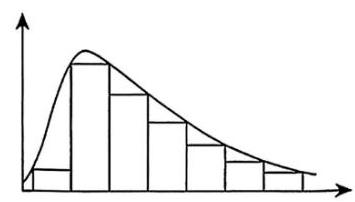
\includegraphics[max width=0.3\textwidth]{images/bo_d6dceus601uc73dvofhg_154_1045_1543_355_202_0.jpg}
\end{center}
\hspace*{3em} 

【答案】B《

5.【2025.12 浦东高三一模 14】某班一次数学小测验(百分制)后，老师为了奖励同学们平时认真学习，决定给每位同学的成绩加上 5 分作为过程性评价奖励. 加分后，与原始分数相比，不会发生改变的是 ( )

A. 平均数 B. 中位数 C. 第 80 百分位数 D. 方差

【答案】D

【答案】每个数据均加 5 , 则平均数、中位数和百分位数也相应增加了 5 , 但方差不变, 故选 D.Z

6.【2025.12 闵行高三一模 19】小闵同学某一天进行了 10 次 100 米短跑集训，其中上午进行了 6 次，下午进行了 4 次.如下是他上午集训 6 次的成绩(单位:s):13.7 13.9 14.9

15.3 12.9 13.3

(1)求这 6 次成绩的中位数；

(2)参考这一天上午集训的数据，用经验概率估计概率，求该同学训练 100 米短跑 3 次至少有一次用时小于 \({13}\mathrm{\;s}\) 的概率;

(3)若该同学下午 4 次的集训原始成绩记录丢失，但记得这 4 次的平均成绩是 \({14.25}\mathrm{\;s}\) ，方差是 0.75 ，求他这一天 10 次训练成绩的平均值和方差.

【答案】(1)13.8

(2) \(\frac{91}{216}\) (3)平均值 14.1 和方差 0.745 .

【解析】(1) \(\frac{{13.7} + {13.9}}{2} = {13.8}\) .

(2)由题意，设该同学训练 100 米短跑每跑 1 次成绩小于 \({13}\mathrm{\;s}\) 为事件 \(A\) ，则 \(P\left( A\right)  = \frac{1}{6}\) ， 设该同学训练 100 米短跑每跑 3 次至少有一次用时小于 \({13}\mathrm{\;s}\) 为事件 \(B\) ，

\(P\left( B\right)  = 1 - P\left( \bar{B}\right)  = 1 - {\left( 1 - P\left( A\right) \right) }^{3} = 1 - {\left( \frac{5}{6}\right) }^{3} = \frac{91}{216}\)

(3)设10次成绩的总平均值为 \(\mu  = \frac{{13.7} + {13.9} + {14.9} + {15.3} + {12.9} + {13.3} + {14.25} \times  4}{10} = {14.1}\) ， 设下午的 4 次成绩分别为 \({y}_{1},{y}_{2},{y}_{3},{y}_{4}\) ,其平均数为 \(\bar{y} = {14.25}\) ,方差是 \({s}_{y}^{2} = {0.75},{10}\) 次成绩的总体方差为 \({s}^{2}\) ,则

\[
{s}^{2} = \frac{1}{10}\left\lbrack  {{\left( {13.7} - {14.1}\right) }^{2} + {\left( {13.9} - {14.1}\right) }^{2} + {\left( {14.9} - {14.1}\right) }^{2} + {\left( {15.3} - {14.1}\right) }^{2} + {\left( {12.9} - {14.1}\right) }^{2}}\right.
\]

\[
\left. {+{\left( {13.3} - {14.1}\right) }^{2} + {\left( {y}_{1} - {14.1}\right) }^{2} + \cdots  + {\left( {y}_{4} - {14.1}\right) }^{2}}\right\rbrack
\]

\[
= \frac{{4.36} + {\left( {y}_{1} - {14.1}\right) }^{2} + \cdots  + {\left( {y}_{4} - {14.1}\right) }^{2}}{10} = \frac{{4.36} + {\left\lbrack  \left( {y}_{1} - \bar{y}\right)  + \left( \bar{y} - {14.1}\right) \right\rbrack  }^{2} + \cdots  + {\left\lbrack  \left( {y}_{4} - \bar{y}\right)  + \left( \bar{y} - {14.1}\right) \right\rbrack  }^{2}}{10}
\]

\[
= \frac{{4.36} + 4{s}_{y}^{2} + {\left( \bar{y} - {14.1}\right) }^{2} \times  4 + 2\left( {\bar{y} - {14.1}}\right) \left\lbrack  {\left( {{y}_{1} - \bar{y}}\right)  + \cdots  + \left( {{y}_{4} - \bar{y}}\right) }\right\rbrack  }{10}
\]

\[
= \frac{{4.36} + 4 \times  {0.75} + {\left( {14.25} - {14.1}\right) }^{2} \times  4 + 0}{10} = {0.745}
\]

7.【2025.12 黄浦高三一模 17】一家水果店的店长为了解本店苹果的日销售情况,记录了过去 20 天苹果的日销售量(单位:kg),按从小到大的排序结果如下:

62,74,75,84,84,85,85,85,86,87,89,92,93,94,97,99,101,104,107,117.

(1)求该水果店过去 20 天苹果日销售量的平均数；

(2)若以过去 20 天苹果的日销售量的第 80 百分位数作为下个月每日苹果的平均进货量，试确定下个月每日苹果的平均进货量;

(3)若从过去 20 天中随机抽取 3 天，分别求“3 天中每天的苹果销售量均超过 90kg”与“3 天中恰有 2 天的苹果销售量超过 90kg”的概率.

【答案】(1)90kg (2)100kg

(3) \(\frac{7}{95},\frac{33}{95}\)

【解析】(1) \(\because \bar{x} = \frac{{x}_{1} + {x}_{2} + {x}_{3} + \cdots  + {x}_{20}}{20} = {90}\) ,

故该水果店过去 20 天苹果日销售量的平均数为 90kg. .4 分

(2) \(\because {20} \cdot  {80}\%  = {16}\) ，故过去 20 天苹果的日销售量的第 80 百分位数为 \(\frac{{99} + {101}}{2} = {100}\) ， 所以下个月每日苹果的平均进货量为 \({100}\mathrm{{kg}}\) . .8 分

(3)过去 20 天苹果的日销售量超过 90kg 共有 9 天，

所以“3 天中每天的苹果销售量均超过 90kg”的概率为 \(\frac{{\mathrm{C}}_{9}^{3}}{{\mathrm{C}}_{20}^{3}} = \frac{7}{95}\) ; .11 分

"3 天中恰有 2 天的苹果销售量超过 90kg"的概率为 \(\frac{{\mathrm{C}}_{9}^{2}{\mathrm{C}}_{11}^{1}}{{\mathrm{C}}_{20}^{3}} = \frac{33}{95}\) . .14 分

8.【2025.12 金山高三一模 17】核桃有很多品种. 小何购买了其中 4 种品类的核桃: \(A\) 类核桃 100 个, \(B\) 类核桃 120 个, \(C\) 类核桃 80 个和 \(D\) 类核桃 200 个.

(1)小何决定采用分层抽样的方法，从所有核桃中抽出 25 个核桃，请问应抽取 \(C\) 类核桃多少个?

(2)小何以随机抽样的方式，从 \(D\) 类核桃中抽取 20 个进行克重测量，以下是这些核桃的克重数据:(单位:克)

\begin{center}
\adjustbox{max width=\textwidth}{
\begin{tabular}{|c|c|c|c|c|c|c|c|c|c|}
\hline
14.4 & 14.7 & 15.2 & 16.3 & 17.3 & 17.6 & 17.9 & 18.2 & 19.0 & 19.3 \\
\cline{1-10}
19.8 & 20.1 & 20.2 & 20.4 & 20.7 & 20.9 & 21.3 & 21.7 & 22.4 & 22.6 \\
\cline{1-10}
\hline
\end{tabular}
}
\end{center}

 \circled{1} 从该 20 个核桃中任取 2 个，则所取 2 个核桃的克重均大于 20 克的概率为多少？

 \circled{2}  记 \(\bar{x}\) 为该 20 个核桃的平均克重， \(s\) 为该 20 个核桃克重的标准差，则该 20 个核桃中有多少个核桃的克重位于 \(\bar{x} - s\) 与 \(\bar{x} + s\) 之间?

\begin{center}
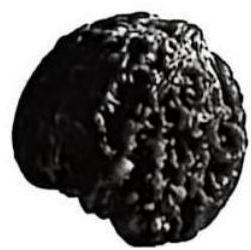
\includegraphics[max width=0.2\textwidth]{images/bo_d6dceus601uc73dvofhg_157_1151_944_251_250_0.jpg}
\end{center}
\hspace*{3em} 

【答案】(1)C 类核桃 4 只

(2) \circled{1}  \(\frac{18}{95}\)  \circled{2} 有 13 个

【解析】(1) 设 \(n\) 为抽取 \(C\) 类核桃的只数,根据分层抽样的方法,有 \(\frac{n}{80} = \frac{25}{{100} + {120} + {80} + {200}},\) .2 分

得到 \(n = 4\) . .4 分

所以 \(C\) 类核桃 4 只.

(2) \circled{1} 因为有 9 个核桃的克重大于 20 克， .6 分

所以 \(P = \frac{{C}_{9}^{2}}{{C}_{20}^{2}} = \frac{18}{95}\) . .9 分

所以所取 2 个核桃的克重均大于 20 克的概率为 \(\frac{18}{95}\) .

 \circled{2} 计算可得: \(x = {19},s = {2.42}\) .12 分

所以 \(\bar{x} - s = {16.58},\bar{x} + s = {21.42}\) ,克重位于 \({16.58}\mathrm{\;g}\) 和 \({21.42}\mathrm{\;g}\) 的核桃有 13 个.

9.【2025.12 嘉定高三一模 17】A 校抽取 66 名高一年级学生测量身高,因某种原因原始数据遗失. 已知该样本是按照分层随机抽样的方法抽取的,其中男生 34 名,身高平均数为 \({173}\mathrm{\;{cm}}\) ; 女生 32 名, 身高平均数为 161cm. 该 66 名学生身高的方差为 60. 其频率分布直方图如下:

(1)求该 66 名学生中身高在 [169.5,172.5) (单位:cm) 内的人数；

(2)试用已知数据估计 A 校高一年级全体学生身高的平均数；何先果精确到 0.1cm

(3)若一组数据落在 \(\left\lbrack  {x - {2s},x + {2s}}\right\rbrack\) ( \(x\) 是平均数， \(s\) 是标准差)内的频率不小于 92\% ，则称这组数据满足“常态”. 试判断这 66 个身高数据是否满足“常态”，并说明理由.

\begin{center}
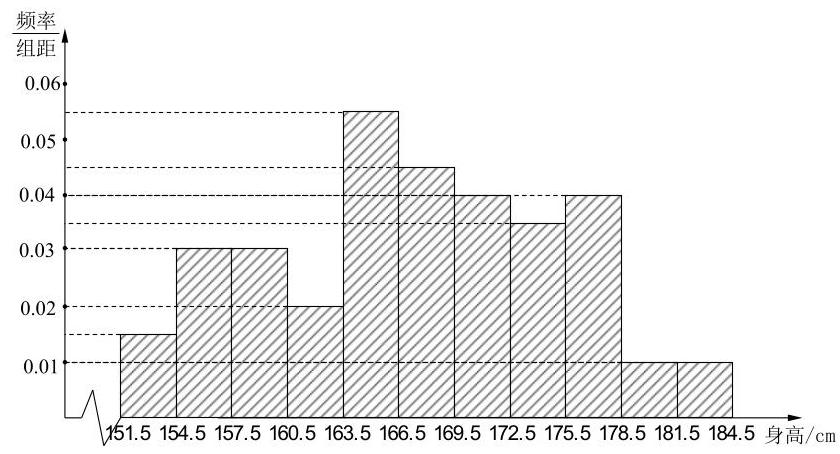
\includegraphics[max width=0.7\textwidth]{images/bo_d6dceus601uc73dvofhg_158_403_681_840_454_0.jpg}
\end{center}
\hspace*{3em} 

【答案】(1)8 (2)167.2cm (3)满足

【解析】(1) 频率分布直方图的组距为 3cm.

因为 \(\lbrack {169.5},{172.5})\) 对应的纵坐标值为 0.04 ，故频率 \(= {0.04} \times  3 = {0.12}\) .

人数=66×0.12≈8(人). 因此，身高在该区间内的人数为 8 人.

(2)样本平均数为: \(\overset{ - }{x} = \frac{{34} \times  {173} + {32} \times  {161}}{66} \approx  {167.2}\left( \mathrm{\;{cm}}\right)\) .

由分层随机抽样原则,可估计总体身高平均数约为 \({167.2}\mathrm{\;{cm}}\) .

(3)已知方差 \({s}^{2} = {60}\) ，则标准差 \(s = \sqrt{60} \approx  {7.75}\) .

平均数 \(\bar{x} \approx  {167.2}\) ,因此区间 \(\left\lbrack  {\bar{x} - {2s},\bar{x} + {2s}}\right\rbrack\) 约为: \(\left\lbrack  {{151.7},{182.7}}\right\rbrack\) .

因此,落在 \(\left\lbrack  {\frac{}{x} - {2s},\frac{}{x} + {2s}}\right\rbrack\) 内的频率 \(= 1 -\) 两侧尾部频率之和.

区间 \(\lbrack {181.5},{184.5})\) 对应的频率为 \({0.01} \times  3 = {0.03}\) ,其中超出 182.7 的部分的频率小于 0.03 .

区间 \(\lbrack {151.5},{154.5})\) 对应的频率约为 \({0.017} \times  3 = {0.051}\) ,其中小于 151.7 的部分的频率远小于 0.05 .

因此，落在区间内的频率>1-(0.03+0.05)=92\%，满足“常态”、“

10.【2025.12 徐汇高三一模 18】某校高三年级学生参加了一次时政知识竞赛，为了了解本次竞赛的成绩情况, 从所有答卷中随机抽取 100 份作为样本进行统计, 将样本的成绩 (满分 100 分, 成绩均为不低于 40 分的整数) 分成六段: \(\lbrack {40},{50}),\lbrack {50},{60}),\ldots ,\left\lbrack  {{90},{100}}\right\rbrack\) 得到如图所示的频率分布直方图.

(1)求实数 \(m\) 的值；若年级准备选取 80 分及以上的学生进入下一轮竞赛，已知该校高三年级有 1000 名学生，估计该校高三年级参加下一轮竞赛的人数；

(2)王老师抽取了 10 名参加竞赛的学生，他们的分数为: \({x}_{1}\) ， \({x}_{2}\) ， \({x}_{3}\) ， \(\cdots\) ， \({x}_{10}\) . 已知这 10 个分数的平均数 \(x = {91}\) ,标准差 \(s = 5\) ,若剔除其中的 96 和 86 这 2 个分数,求剩余 8 个分数的平均数与方差.

\begin{center}
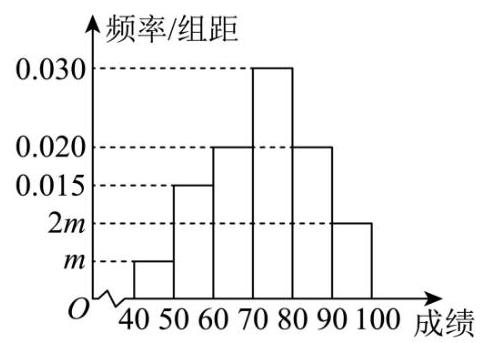
\includegraphics[max width=0.4\textwidth]{images/bo_d6dceus601uc73dvofhg_159_924_826_481_343_0.jpg}
\end{center}
\hspace*{3em} 

【答案】(1)300 人 (2)平均数为 91，方差为 25 .

【解析】(1) 由题意知, \(\left( {{0.030} + {0.020} \times  2 + {0.015} + {2m} + m}\right)  \times  {10} = 1\) ,所以 \(m = {0.005}\) . 该校高一年级参加下一轮竞赛的人数估计为 \({1000} \times  \left( {{0.020} + {0.005} \times  2}\right)  \times  {10} = {300}\) 人.

(2)因为 \(\bar{x} = {91}\) ，所以 \({x}_{1} + {x}_{2} + \cdots  + {x}_{10} = {10} \times  {91} = {910}\) ，

所以 \({s}^{2} = \frac{1}{10}\left( {{x}_{1}^{2} + {x}_{2}^{2} + \cdots  + {x}_{10}^{2}}\right)  - {91}^{2} = {5}^{2}\) ,所以 \({x}_{1}^{2} + {x}_{2}^{2} + \cdots  + {x}_{10}^{2} = {83060}\) .

剔除其中的 96 和 86 这 2 个分数,设剩余 8 个分数为 \({x}_{1},{x}_{2},{x}_{3},\cdots ,{x}_{8}\) ,平均数与标准差分别为 \(\overline{{x}_{0}},{s}_{0}\) ,则剩余 8 个分数的平均数 \(\overline{{x}_{0}} = \frac{{x}_{1} + {x}_{2} + {x}_{3} + \cdots  + {x}_{8}}{8} = \frac{{910} - {96} - {86}}{8} = {91}\) ,

方差 \({s}_{0}^{2} = \frac{1}{8}\left( {{x}_{1}^{2} + {x}_{2}^{2} + \cdots  + {x}_{8}^{2}}\right)  - {91}^{2} = \frac{1}{8}\left( {{83060} - {96}^{2} - {86}^{2}}\right)  - {91}^{2} = {25}\) .

所以剩余 8 个分数的平均数为 91 ，方差为 25 . \(>\)

11.【2025.12 杨浦高三一模 19】为了了解某校高三年级学生的体育成绩，随机选取 100 名学生参加考核, 将考核的成绩 (满分 100 分, 成绩均为不低于 40 分的整数) 分成六组: \(\lbrack {40},{50}),\lbrack {50},{60}),\lbrack {60},{70}),\lbrack {70},{80}),\left\lbrack  {{80},{90}),\left\lbrack  {{90},{100}}\right\rbrack  ,\text{ 得到如图所示的频率分布直方图. }}\right\rbrack\)

(1)求频率分布直方图中 \(a\) 的值;

(2)在考核成绩为 \(\lbrack {70},{80}),\lbrack {80},{90}),\left\lbrack  {{90},{100}}\right\rbrack\) 的三组学生中,用分层抽样的方法抽取 13 人, 则考核成绩在 \(\lbrack {70},{80})\) 中的学生应抽取多少人?

(3)若落在 \(\lbrack {50},{60})\) 学生的平均成绩是54.4，方差是5.2，落在 \(\lbrack {60},{70})\) 学生的平均成绩为 66.4， 方差是 9.2 ，求这两组学生成绩的平均数和方差. (结果精确到 0.1)

\begin{center}
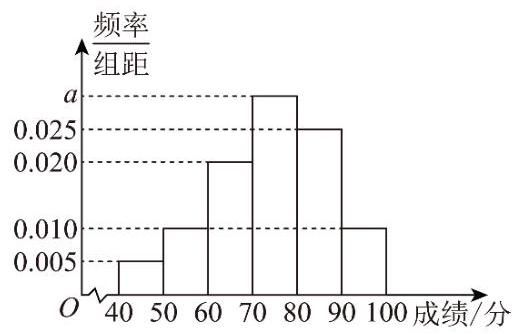
\includegraphics[max width=0.4\textwidth]{images/bo_d6dceus601uc73dvofhg_160_888_811_514_334_0.jpg}
\end{center}
\hspace*{3em} 

【答案】(1) \(a = {0.03}\) (2)6 人 (3) \(\bar{z} = {62.4},{s}^{2} = {39.9}\)

【解析】(1) 由频率之和为 1 结合频率分布直方图可得

\({10} \times  \left( {{0.005} + {0.01} + {0.02} + a + {0.025} + {0.01}}\right)  = 1\) ,解得 \(a = {0.03},4\) 分

(2)由频率分布直方图知，样本答卷成绩在 \(\lbrack {70},{80}),\lbrack {80},{90}),\lbrack {90},{100})\) 的三组学生有 \({100} \times  {10} \times  \left( {{0.03} + {0.025} + {0.01}}\right)  = {65}\) (人),

其中样本答卷成绩在 [70,80) 的学生人数为 \({100} \times  {10} \times  {0.03} = {30},6\) 分

用分层抽样的方法应从答卷成绩在 \(\lbrack {70},{80})\) 的学生中抽取 \(\frac{30}{65} \times  {13} = 6\) (人) 8 分

(3)由频率分布直方图知，成绩在 \(\lbrack {50},{60})\) 的学生人数为 \({100} \times  {0.1} = {10}\) ，

成绩在 \(\lbrack {60},{70})\) 的学生人数为 \({100} \times  {0.2} = {20},{10}\) 分

所以两组学生成绩的平均数 \(\bar{z} = \frac{{10} \times  {54.4} + {20} \times  {66.4}}{{10} + {20}} = {62.4},{12}\) 分

两组学生成绩的方差 \({s}^{2} = \frac{10}{{10} + {20}}\left\lbrack  {{5.2} + {\left( {54.4} - {62.4}\right) }^{2}}\right\rbrack   + \frac{20}{{10} + {20}}\left\lbrack  {{9.2} + {\left( {66.4} - {62.4}\right) }^{2}}\right\rbrack   = {39.9}\)

12.【2025.12 虹口高三一模 19】班主任小明为了解本班每位学生每周平均手机使用时长(单位:小时), 在某一学期每周对全班 45 名学生进行问卷调查,收集了全部数据并计算出每位学生每周平均手机使用时长,绘制了相应的统计图表, 全班用时最长的为 25.6 小时.其中, 男生每周平均手机使用时长的茎叶图如图 19-1 所示, 女生每周平均手机使用时长的频率分布直方图如图 19-2 所示.

\begin{center}
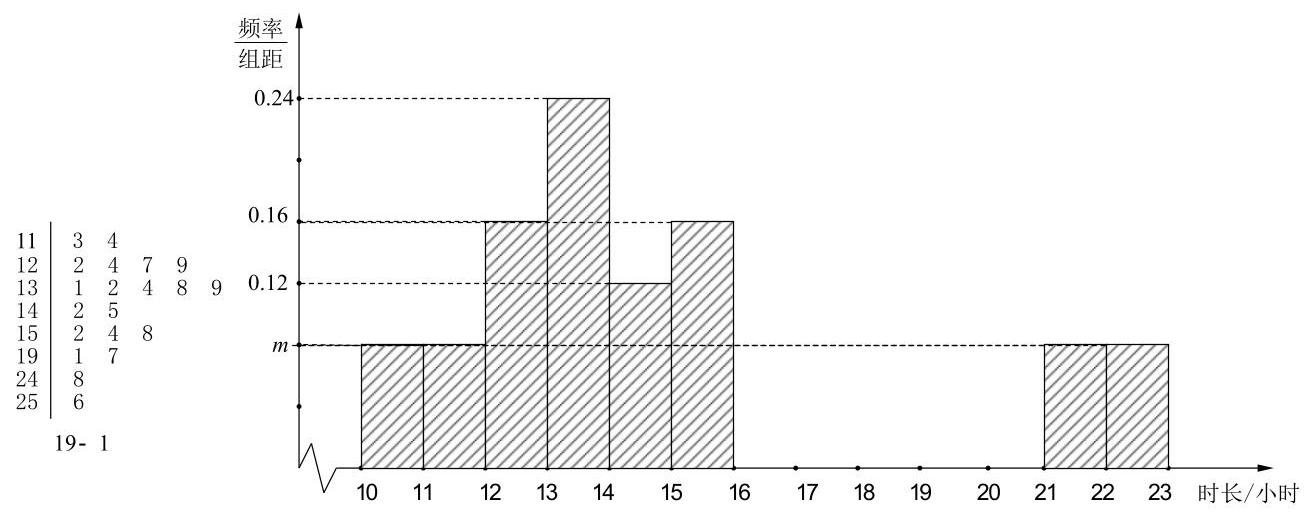
\includegraphics[max width=1.0\textwidth]{images/bo_d6dceus601uc73dvofhg_161_240_587_1304_515_0.jpg}
\end{center}
\hspace*{3em} 

19 -2

(1)求该班男生每周平均手机使用时长的第 25 百分位数；

(2)小明老师想从本班每周平均手机使用时长 小于 12 小时的学生中任选 2 人在班会课上做经验分享. 设事件 \(A\) 表示“2 人中至多 1 名男生”,事件 \(B\) 表示“2 人中恰有 1 名学生的每周平均手机使用时长位于区间 \(\lbrack {11},{12})\) ”. 试判断事件 \(A\) 和事件 \(B\) 是否独立,并说明理由:

(3)小明老师发现本班有 \(t\) 位学生的每周平均手机使用时长超过 20 小时，这 \(t\) 位学生的数据平均数为 23 小时.当去掉这 \(t\) 位学生中用时最长和用时最短的数据后,平均数变为 22.7 小时, 且这 \(t\) 位学生中女生的数据从小到大依次排序成等差数列. 那么这 \(t\) 位学生每周平均手机使用时长的方差是否超过 3?请说明理由.

【答案】(1)12.8 (2)不独立 (3)没有超过

【解析】(1) 由题,男生有 20 人，则指标 \(i = 5\) ,

所以第 25 百分位数为 \(\frac{{12.7} + {12.9}}{2} = {12.8}\) . 2 分

(2) \({4m} + {0.12} + {0.16} + {0.16} + {0.24} = 1\) ，所以 \(m = {0.08}.4\) 分

则男生中有 2 人用时小于 12 小时, 女生有 2 人用时位于[10,11), 有 2 人同时位于[11,12). 所以 \(P\left( A\right)  = \frac{{\mathrm{C}}_{4}^{2} + {\mathrm{C}}_{2}^{1} \cdot  {\mathrm{C}}_{4}^{1}}{{\mathrm{C}}_{6}^{2}} = \frac{14}{15},P\left( B\right)  = \frac{{\mathrm{C}}_{2}^{1} \cdot  {\mathrm{C}}_{4}^{1}}{{\mathrm{C}}_{6}^{2}} = \frac{8}{15},P\left( {A \cap  B}\right)  = \frac{{\mathrm{C}}_{2}^{1} \cdot  {\mathrm{C}}_{2}^{1} + {\mathrm{C}}_{2}^{1} \cdot  {\mathrm{C}}_{2}^{1}}{{\mathrm{C}}_{6}^{2}} = \frac{8}{15}\) ,

由于 \(P\left( {A \cap  B}\right)  \neq  P\left( A\right) P\left( B\right)\) ,故事件 \(A\) 和事件 \(B\) 不独立. 8 分

(3)由题， \(t = 6\) ，其中 2 位男生，4 位女生. 设这四位女生的用时依次为 \({a}_{1}\) 、 \({a}_{2}\) 、 \({a}_{3}\) 、 \({a}_{4}\) . 则 \(\left\{  \begin{array}{l} {23} \times  6 = {a}_{1} + {a}_{2} + {a}_{3} + {a}_{4} + {24.8} + {25.6}, \\  {22.7} \times  4 = {a}_{2} + {a}_{3} + {a}_{4} + {24.8}, \end{array}\right.\) 10 分

解得 \({a}_{1} = {21.6}\) ,设公差为 \(d\) ,则 \(d = {0.2}.{12}\) 分

故 \({s}^{2} = \frac{1}{6}\left( {{\left( {24.8} - {23}\right) }^{2} + {\left( {25.6} - {23}\right) }^{2} + \mathop{\sum }\limits_{{i = 1}}^{4}{\left( {a}_{i} - {23}\right) }^{2}}\right)  = \frac{188}{75} < 3\) ,没有超过. 14 分

13.【2025.12 青浦高三一模 19】随着手机和网络的普及, 外卖行业得到迅速发展. 某外卖平台为了解某地区用户对其提供的服务的满意度，随机调查了 40 个用户，得到用户的满意度评分, 系统自动将评分按从大到小顺序排列如下:

\begin{center}
\adjustbox{max width=\textwidth}{
\begin{tabular}{|c|c|c|c|c|c|c|c|c|c|}
\hline
用户编号 & 评分 & 用户编号 & 评分 & 用户编号 & 评分 & 用户编号 & 评分 & 用户编号 & 评分 \\
\cline{1-10}
01 & 97 & 09 & 88 & 17 & 83 & 25 & 79 & 33 & 76 \\
\cline{1-10}
02 & 96 & 10 & 88 & 18 & 83 & 26 & 79 & 34 & 75 \\
\cline{1-10}
03 & 95 & 11 & 86 & 19 & 82 & 27 & 78 & 35 & 74 \\
\cline{1-10}
04 & 93 & 12 & 86 & 20 & 82 & 28 & 78 & 36 & 74 \\
\cline{1-10}
05 & 92 & 13 & 85 & 21 & 81 & 29 & 78 & 37 & 73 \\
\cline{1-10}
06 & 91 & 14 & 85 & 22 & 81 & 30 & 77 & 38 & 72 \\
\cline{1-10}
07 & 89 & 15 & 84 & 23 & 81 & 31 & 76 & 39 & 66 \\
\cline{1-10}
08 & 89 & 16 & 84 & 24 & 80 & 32 & 76 & 40 & 63 \\
\cline{1-10}
\hline
\end{tabular}
}
\end{center}

(1)求这组数据的极差和第 95 百分位数.

(2)若从这 40 个用户中抽取一个容量为 10 的样本，有一个数据不小心丢失了，抽到的其他 9 个用户的评分分别为 92, 84, 86, 78, 89, 74, 78, 77, 89 , 且这 10 个数据的平均数 \(\bar{x} = {83}\) . 记这 10 个数据的方差为 \({s}^{2}\) ,若用户的满意度评分在区间 \(\left( {\bar{x} - s,\bar{x} + s}\right)\) 上,则满意度等级为“ \(A\) 级”. 从这 10 个数据里面任取 3 个,求恰有 2 个满意度等级为“ \(A\) 级”的概率.

(3)平台为拓展客流，开发了一个新的评价系统. 把(2)中样本的平均数和方差作为老评价系统的数据,且老系统的样本容量占两个系统所有样本容量的 \(\frac{1}{3}\) ,新系统得出的评分平均数为 89 分, 方差为 12. 据此计算新老系统所有评分的方差.

【答案】(1)95.5 ，极差为 34. (2) \(\frac{{C}_{5}^{2}{C}_{5}^{1}}{{C}_{10}^{3}} = \frac{5}{12}\) (3)方差为 27

【解析】(1) 将所有用户评分按从小到大排列

由题表可知这 40 个用户评分按从小到大排列如下:63,66,72,73,74,74,75,76,76, 76,77,78,78,78,79,79,80,81,81,81,82,82,83,83,84,84,85,85,86, 86,88,88,89,89,91,92,93,95,96,97.

因为 \({40} \times  {95}\%  = {38}\) ,所以这 40 个用户评分的 95\% 分位数为第 38 个数和第 39 个数据的平均数， \(\frac{{95} + {96}}{2} = {95.5}\) ，极差为 \({97} - {63} = {34}\) .

(2)设丢失的数据为 \(m\) ，

则 \(\bar{x} = \frac{1}{10}\left( {{92} + {84} + {86} + {78} + {89} + {74} + {78} + {77} + {89} + m}\right)  = {83}\) ,解得 \(m = {83}\) . 所以 \({s}^{2} = \frac{1}{10}\left\lbrack  {{\left( {92} - {83}\right) }^{2} + {\left( {84} - {83}\right) }^{2} + {\left( {86} - {83}\right) }^{2} + {\left( {78} - {83}\right) }^{2} + {\left( {89} - {83}\right) }^{2}}\right. \; \left. {+{\left( {74} - {83}\right) }^{2} + {\left( {78} - {83}\right) }^{2} + {\left( {77} - {83}\right) }^{2} + {\left( {89} - {83}\right) }^{2} + {\left( {83} - {83}\right) }^{2}}\right\rbrack   = {33}\) 由题意知评分在 \(\left( {{83} - \sqrt{33},{83} + \sqrt{33}}\right)\) ,即 \(\left( {{77.26},{88.74}}\right)\) 内的满意度等级为 “A 级”, 所以 10 个样本数据中评分在 \(\left( {{77.26},{88.74}}\right)\) 内的有 5 个,故所求概率为 \(\frac{{C}_{5}^{2}{C}_{5}^{1}}{{C}_{10}^{3}} = \frac{5}{12}\)

(3)设老系统的平均数与方差分别为 \(\overline{{x}_{1}}\) ， \({s}_{1}^{2}\) ，新系统的平均数与方差分别为 \(\overline{{x}_{2}}\) ， \({s}_{2}^{2}\) ，新老系统所有评分的平均数与方差分别为 \(\overline{{x}_{0}},{s}_{0}^{2}\) ,由题意知 \(\overline{{x}_{1}} = {83},\overline{{x}_{2}} = {89},{s}_{1}^{2} = {33},{s}_{2}^{2} = {12}\) . 因为老系统的总数据占两个系统所有数据总和的 \(\frac{1}{3}\) ,假设老系统有 \(n\) 个数据,则新系统有 \({2n}\) 个数据,所以新老系统所有评分的平均数 \(\overline{{x}_{0}} = \frac{n\overline{{x}_{1}} + {2n}\overline{{x}_{2}}}{3n} = {87}\) ,

方差 \({s}_{0}^{2} = \frac{1}{3n}\left\lbrack  {\mathop{\sum }\limits_{{i = 1}}^{n}{\left( {x}_{i} - {87}\right) }^{2} + \mathop{\sum }\limits_{{j = 1}}^{{2n}}{\left( {x}_{j} - {87}\right) }^{2}}\right\rbrack   = \frac{1}{3n}\left\{  {\mathop{\sum }\limits_{{i = 1}}^{n}{\left\lbrack  \left( {x}_{i} - \overline{{x}_{1}}\right)  + \left( \overline{{x}_{1}} - {87}\right) \right\rbrack  }^{2} + \mathop{\sum }\limits_{{j = 1}}^{{2n}}{\left\lbrack  \left( {x}_{j} - \overline{{x}_{2}}\right)  + \left( \overline{{x}_{2}} - {87}\right) \right\rbrack  }^{2}}\right\} \; = \frac{1}{3}\left\{  {\left\lbrack  {{33} + {\left( {83} - {87}\right) }^{2}}\right\rbrack   + 2\left\lbrack  {{12} + {\left( {89} - {87}\right) }^{2}}\right\rbrack  }\right\}   = {27}\) ,即新老系统所有评分的方差为 27. \(\propto\)

\section*{10.3 茎叶图}

1.【2025.12 松江高三一模 5】某运动员在某次男子 10 米气手枪射击比赛中的得分数据 (单位: 环) 如茎叶图所示, 则这组数据的平均数为\_\_\_\_\_.

\begin{center}
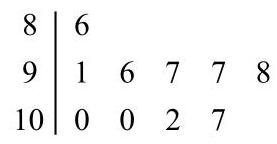
\includegraphics[max width=0.2\textwidth]{images/bo_d6dceus601uc73dvofhg_164_1126_390_277_144_0.jpg}
\end{center}
\hspace*{3em} 

【答案】9.74

【解析】平均数为 \(\bar{x} = \frac{{8.6} + {9.1} + {9.6} + {9.7} + {9.7} + {9.8} + {10.0} + {100} + {10.2} + {10.7}}{10} = {9.74}\) .

2.【2025.12 徐汇高三一模 14】用简单随机抽样的方法抽取某个品种的小麦样本 13 株, 测得麦穗长度(单位:cm)，以其整数部分作为“茎”，小数部分作为“叶”绘制茎叶图如右图所示. 用该样本数据估计此品种小麦麦穗长度平均为( ). (结果精确到 \({0.1}\mathrm{\;{cm}}\) )

\begin{center}
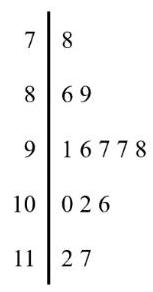
\includegraphics[max width=0.2\textwidth]{images/bo_d6dceus601uc73dvofhg_164_1225_898_153_292_0.jpg}
\end{center}
\hspace*{3em} 

A. 9.9cm B. 9.8cm C. 9.7cm D. 9.6cm

【答案】平均数为

\(\frac{{7.8} + {8.6} + {8.9} + {9.1} + {9.6} + {9.7} + {9.7} + {9.8} + {10.0} + {10.2} + {10.6} + {11.2} + {11.7}}{13} \approx  {9.8}\) ,所以选 B. \(\ll\)

3.【2025.12 宝山高三一模 18】某场篮球比赛中, 甲、乙两队各 5 名队员进行比赛, 他们得分的茎叶图如图,已知 \(x,y \in  N\) ,且 \(4 \leq  x \leq  9,6 \leq  y \leq  9\) .

(1)若甲队队员得分的极差为 32，乙得分的平均值为 24，求其中 \(x\) 和 \(y\) 的值；

(2)从得分在 20 分及以上的队员中随机抽取 2 名，求至少有 1 名来自乙队的概率；

(3)若甲乙两队的队员平均分相等，求 \(x + \frac{50}{y}\) 的最大值，并写出此时 \(x\) 和 \(y\) 的值.

\begin{center}
\adjustbox{max width=\textwidth}{
\begin{tabular}{|c|c|c|}
\hline
甲 & \phantom{X} & 乙 \\
\cline{1-3}
6 & 0 & \phantom{X} \\
\cline{1-3}
4 & 1 & 2 \\
\cline{1-3}
8 & 2 & 5 6 \(y\) \\
\cline{1-3}
\(x\) 4 & 3 & 1 \\
\cline{1-3}
\hline
\end{tabular}
}
\end{center}

【答案】(1) \(x = 8,y = 6\) (2) \(\frac{6}{7}\) (3)最大值为 \(\frac{49}{3}\) ，此时 \(x = 8,y = 6\)

【解析】(1) 极差为 32,则 \({30} + x - 6 = {32}\) ,解得 \(x = 8\)

乙得分的平均值为 24,则 \(\frac{1}{5}\left( {{12} + {25} + {26} + {20} + y + {31}}\right)  = {24}\) ,解得 \(y = 6\)

( 2 )得分在 20 分及以上的队员，甲队有 3 名. 乙队有 4 名.

从而随机抽取 2 名学生, 至少有 1 名来自乙队的概率:

\(P\left( A\right)  = \frac{{C}_{3}^{1}{C}_{4}^{1} + {C}_{4}^{2}}{{C}_{7}^{2}} = \frac{6}{7}\) 或 \(P\left( A\right)  = 1 - \frac{{C}_{3}^{2}}{{C}_{7}^{2}} = \frac{6}{7}\)

(3)甲乙两队的平均分相等,则 \(6 + {14} + {28} + {34} + {30} + x = {12} + {25} + {26} + {20} + y + {31}\)

可得 \(x = y + 2\) ,所以 \(x + \frac{50}{y} = y + \frac{50}{y} + 2\) ,

又因为 \(x,y \in  N\) 且 \(4 \leq  x \leq  9,6 \leq  y \leq  9\) ,从而 \(8 \leq  y + 2 \leq  9\) ,所以 \(y = 6\) 或 7

当 \(y = 7\) 时, \(x = 9,x + \frac{50}{y} = \frac{113}{7}\) ,当 \(y = 6\) 时, \(x = 8,x + \frac{50}{y} = \frac{49}{3}\)

所以 \(x + \frac{50}{y}\) 的最大值为 \(\frac{49}{3}\) ,此时 \(x = 8,y = 6\) . \&

4.【2025.12 奉贤高三一模 18】A 校高一年级共有学生 462 名，其中女生 224 名. 为了解该校高一年级学生的身高和体重情况，按分层随机抽样从中获取 66 名学生的身高(cm)和体重(kg)，其中 66 名学生的身高(从低到高排序三列，每列 22 人)汇总如左下表(隐蔽部分信息数据)，身高的频率分布表如右下表(隐蔽了部分信息数据)，66 名学生体重绘制茎叶图如右下图.

(1)能否推算出身高 \({165}\mathrm{\;{cm}}\) 的具体人数？

(2)求抽取的男生人数、抽取到的男生体重的中位数；

(3)已知这 66 名学生中男生身高平均数为 173.1cm，方差为 25.9；女生身高平均数为 161.3cm， 方差为 23.3. 请计算该样本数据在区间 \(\left\lbrack  {\bar{x} - {2s},\bar{x} + {2s}}\right\rbrack\) 中包含样本数据的个数.

(其中 \(x\) 是样本平均数, \(s\) 是样本标准差)

A 校 66 名高一年级学生身高数据

\begin{center}
\adjustbox{max width=\textwidth}{
\begin{tabular}{|c|c|c|c|c|c|}
\hline
性别 & 身高/cm & 性别 & 身高/cm & 性别 & 身高/cm \\
\cline{1-6}
女 & 152 & 女 & 164 & 男 & 172 \\
\cline{1-6}
女 & 153 & 男 & 165 & 男 & 172 \\
\cline{1-6}
女 & 154 & \phantom{X} & \phantom{X} & 女 & 172 \\
\cline{1-6}
女 & 155 & \phantom{X} & \phantom{X} & 男 & 173 \\
\cline{1-6}
女 & 156 & \phantom{X} & \phantom{X} & 男 & 173 \\
\cline{1-6}
女 & 156 & \phantom{X} & \phantom{X} & 男 & 174 \\
\cline{1-6}
女 & 156 & \phantom{X} & \phantom{X} & 男 & 174 \\
\cline{1-6}
女 & 157 & \phantom{X} & \phantom{X} & 男 & 174 \\
\cline{1-6}
女 & 157 & \phantom{X} & \phantom{X} & 男 & 174 \\
\cline{1-6}
女 & 159 & \phantom{X} & \phantom{X} & 男 & 175 \\
\cline{1-6}
女 & 159 & \phantom{X} & \phantom{X} & 男 & 176 \\
\cline{1-6}
女 & 160 & \phantom{X} & \phantom{X} & 男 & 176 \\
\cline{1-6}
女 & 160 & \phantom{X} & \phantom{X} & 男 & 177 \\
\cline{1-6}
女 & 160 & \phantom{X} & \phantom{X} & 男 & 177 \\
\cline{1-6}
女 & 160 & \phantom{X} & \phantom{X} & 男 & 178 \\
\cline{1-6}
女 & 161 & \phantom{X} & \phantom{X} & 男 & 178 \\
\cline{1-6}
女 & 162 & \phantom{X} & \phantom{X} & 男 & 178 \\
\cline{1-6}
女 & 163 & 男 & 170 & 男 & 178 \\
\cline{1-6}
女 & 163 & 男 & 170 & 男 & 179 \\
\cline{1-6}
女 & 164 & 男 & 170 & 男 & 181 \\
\cline{1-6}
女 & 164 & 男 & 170 & 男 & 182 \\
\cline{1-6}
女 & 164 & 男 & 170 & 男 & 184 \\
\cline{1-6}
\hline
\end{tabular}
}
\end{center}

A 校 66 名高一年级学生身高的频率分布表

\begin{center}
\adjustbox{max width=\textwidth}{
\begin{tabular}{|c|c|c|c|c|}
\hline
身高分组区间 & 频数 & \phantom{X} & 频率 & 累积频数 \\
\cline{1-5}
\(\lbrack {151.5},{154.5})\) & 3 & \phantom{X} & 0.05 & 3 \\
\cline{1-5}
\(\lbrack {154.5},{157.5})\) & \phantom{X} & \phantom{X} & 0.09 & 9 \\
\cline{1-5}
\(\lbrack {157.5},{160.5})\) & \phantom{X} & \phantom{X} & 0.09 & 15 \\
\cline{1-5}
\(\lbrack {160.5},{163.5})\) & \phantom{X} & \phantom{X} & \phantom{X} & 19 \\
\cline{1-5}
\(\lbrack {163.5},{166.5})\) & \phantom{X} & \phantom{X} & \phantom{X} & 31 \\
\cline{1-5}
\(\lbrack {166.5},{169.5})\) & \phantom{X} & \phantom{X} & \phantom{X} & 39 \\
\cline{1-5}
\(\left\lbrack  {{169.5},{172.5}}\right)\) & \phantom{X} & \phantom{X} & \phantom{X} & 47 \\
\cline{1-5}
\(\lbrack {172.5},{175.5})\) & \phantom{X} & \phantom{X} & \phantom{X} & 54 \\
\cline{1-5}
\(\lbrack {175.5},{178.5})\) & 8 & \phantom{X} & 0.12 & 62 \\
\cline{1-5}
\(\lbrack {178.5},{181.5})\) & 2 & \phantom{X} & 0.03 & 64 \\
\cline{1-5}
\(\left\lbrack  {{181.5},{184.5}}\right\rbrack\) & 2 & \phantom{X} & 0.03 & 66 \\
\cline{1-5}
\hline
\end{tabular}
}
\end{center}

\begin{center}
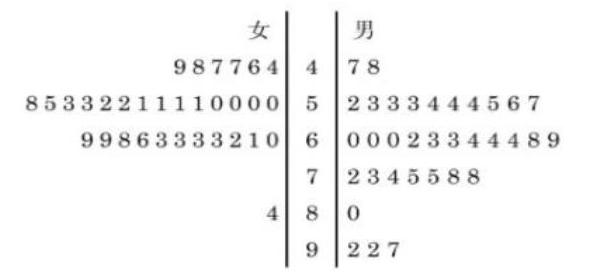
\includegraphics[max width=0.5\textwidth]{images/bo_d6dceus601uc73dvofhg_166_820_697_589_278_0.jpg}
\end{center}
\hspace*{3em} 

A 校 66 名高一年级学生体重的茎叶图

【答案】(1)不能(2)抽取的男生人

数为 34 人、抽取到的男生体重的中位数为 \({63}\mathrm{\;{kg}}\) (3)65 人

【解析】(1) 无法推算

(2)由茎叶图知抽取的男生共 34 人，男生体重的中位数是 63 人.

(3) \(\bar{x} = {167.379}\) 所以 \(s = {7.708}\) . 所以在区间 \(\left\lbrack  {{151.963},{182.795}}\right\rbrack\) 共有 65 人. \(\ll\)

5.【2025.12 崇明高三一模 19】为培养学生的社会责任感, 某校开展了为期一学期的“温暖社区, 青春奉献”志愿服务活动. 活动结束后, 学校从甲、乙两个班级中统计了部分学生的志愿服务时长 (单位:小时)，统计结果用茎叶图记录如图所示 (十位数字作为“茎”，个位数字作为“叶”). 已知甲组有 9 名学生的数据，乙组有 10 名学生的数据.

(1)分别写出甲、乙两组学生服务时长的第 70 百分位数；

(2)从甲、乙两组学生中各随机抽取 1 人，求抽取的 2 人中恰有 1 人的服务时长超过 30 小时的概率;

(3)记甲组志愿服务时长的方差为 \({s}_{0}^{2}\) ；在甲组中增加一名学生 \(A\) 得到“新甲组”，若 \(A\) 的志愿服务时长为 27 ，则记“新甲组”志愿服务时长的方差为 \({s}_{1}^{2}\) ；若 \(A\) 的志愿服务时长为 20 ，则记“新甲组”志愿服务时长的方差为 \({s}_{2}^{2}\) ；通过计算比较 \({s}_{0}^{2}\) 、 \({s}_{1}^{2}\) 、 \({s}_{2}^{2}\) 的大小(结果精确到 0.1)， 并从数学角度解释这一现象.

\begin{center}
\adjustbox{max width=\textwidth}{
\begin{tabular}{|c|c|c|c|c|c|c|c|c|c|c|}
\hline
\multicolumn{5}{|c|}{甲} & \multicolumn{5}{|c|}{乙} & \phantom{X} \\
\cline{1-11}
\phantom{X} & \phantom{X} & \phantom{X} & \phantom{X} & 8 & 1 & 2 & 5 & \phantom{X} & \phantom{X} & \phantom{X} \\
\cline{1-11}
9 & 5 & 5 & 3 & 1 & 2 & 0 & 1 & 4 & 8 & 9 \\
\cline{1-11}
\phantom{X} & \phantom{X} & 6 & 4 & 2 & 3 & 2 & 5 & 6 & \phantom{X} & \phantom{X} \\
\cline{1-11}
\hline
\end{tabular}
}
\end{center}

【答案】(1)32,30.5 (2) \(\frac{13}{30}\)

(3) \({s}_{0}^{2} = \frac{300}{9} \approx  {33.3}\text{ 、 }{s}_{1}^{2} = {30}\text{ 、 }{s}_{2}^{2} = {34.41}\) ，数据波动越大，方差越大，反之越小

【解析】(1) 甲组共 \(9 \curlywedge  9 \times  {0.7} = {6.3}\) ,乙组共 10 人, \({10} \times  {0.7} = 7\) ,

所以甲组第 70 百分位数为 32,乙组第 70 百分位数为 \(\frac{{29} + {32}}{2} = {30.5}\) .4 分

(2)甲组、乙组中各有 3 人服务时长超过 30 小时，

所以恰有 1 人的服务时长超过 30 小时的概率 \(P = \frac{{C}_{3}^{1}{C}_{7}^{1} + {C}_{6}^{1}{C}_{3}^{1}}{{C}_{9}^{1}{C}_{10}^{1}} = \frac{13}{30}\) .5 分

(3) \({s}_{0}^{2} = \frac{1}{9}\mathop{\sum }\limits_{{i = 1}}^{9}{\left( {x}_{i} - \bar{x}\right) }^{2} = \frac{100}{3}\) ，同理 \({s}_{1}^{2} = {30}\) ， \({s}_{2}^{2} = {34.41}\) .3 分

由于甲组均值为 27 ，方差反映了数据的离散程度，当增加数据 27(原样本均值)， 数据相对更集中，方差变小；当增加数据 20，数据更加分散，方差变大……5 分

\section*{第十一章 导数}

\section*{【知识梳理】}

1. 导数的概念

(1)平均变化率:函数 \(y = f\left( x\right)\) 从 \({x}_{0}\) 到 \({x}_{0} + h\) 的平均变化率为 \(\frac{f\left( {{x}_{0} + h}\right)  - f\left( {x}_{0}\right) }{h}\) ；

(2)函数 \(y = f\left( x\right)\) 在 \(x = {x}_{0}\) 处的导数:函数 \(y = f\left( x\right)\) 在 \(x = {x}_{0}\) 的瞬时变化率 \(\mathop{\lim }\limits_{{h \rightarrow  0}}\frac{f\left( {{x}_{0} + h}\right)  - f\left( {x}_{0}\right) }{h}\) ,通常称为 \(y = f\left( x\right)\) 在 \(x = {x}_{0}\) 处的导数,并记作 \({f}^{\prime }\left( {x}_{0}\right)\) ,即 \({f}^{\prime }\left( {x}_{0}\right)  = \mathop{\lim }\limits_{{h \rightarrow  0}}\frac{f\left( {{x}_{0} + h}\right)  - f\left( {x}_{0}\right) }{h}.\)

注意; (1) 这里的增量 \(h\) 不是一般意义上的增量,它可正也可负;

(2)瞬时变化率与导数是同一概念的两个名称；

(3) \({f}^{\prime }\left( {x}_{0}\right)\) 与 \({x}_{0}\) 的值有关，不同的 \({x}_{0}\) 其导数值一般也不相同.

2. 导数的几何意义

函数 \(y = f\left( x\right)\) 在点 \({x}_{0}\) 处的导数 \({f}^{\prime }\left( {x}_{0}\right)\) 的几何意义是曲线 \(y = f\left( x\right)\) 在点 \(\left( {{x}_{0},f\left( {x}_{0}\right) }\right)\) 处的切线的斜率. 曲线在点 \(P\left( {{x}_{0},f\left( {x}_{0}\right) }\right)\) 处的切线方程是 \(y - f\left( {x}_{0}\right)  = {f}^{\prime }\left( {x}_{0}\right) \left( {x - {x}_{0}}\right)\) .

注意:(1)在求曲线的切线方程时,要注意区分所求切线是曲线上某点处的切线,还是过某点的切线:曲线上某点处的切线只有一条,而过某点的切线不一定只有一条,即使此点在曲线上也不一定只有一条;

线上,只有当此点在曲线上时,此点处的切线的斜率才是 \({f}^{\prime }\left( x\right)\) .

3.基本初等函数的导数

(1) \({C}^{\prime } = 0\) (C为常数); (2) \({\left( {x}^{\alpha }\right) }^{\prime } = \alpha {x}^{\alpha  - 1}\) ( \(\alpha\) 是常数); (3) \({\left( {e}^{x}\right) }^{\prime } = {e}^{x}\) ；

(4) \({\left( \ln x\right) }^{\prime } = \frac{1}{x}\) ; (5) \({\left( \sin x\right) }^{\prime } = \cos x\) ; (6) \({\left( \cos x\right) }^{\prime } =  - \sin x\) .

4. 导数的四则运算

若 \(f\left( x\right) ,g\left( x\right)\) 有导数,则: (1) \({\left\lbrack  C \cdot  f\left( x\right) \right\rbrack  }^{\prime } = C{f}^{\prime }\left( x\right) ;\;\left( 2\right) {\left\lbrack  f\left( x\right)  \pm  g\left( x\right) \right\rbrack  }^{\prime } = {f}^{\prime }\left( x\right)  \pm  {g}^{\prime }\left( x\right)\) ;

(3) \({\left\lbrack  f\left( x\right)  \cdot  g\left( x\right) \right\rbrack  }^{\prime } = {f}^{\prime }\left( x\right) g\left( x\right)  + f\left( x\right) {g}^{\prime }\left( x\right)\) ; (4) \({\left\lbrack  \frac{f\left( x\right) }{g\left( x\right) }\right\rbrack  }^{\prime } = \frac{{f}^{\prime }\left( x\right) g\left( x\right)  - f\left( x\right) {g}^{\prime }\left( x\right) }{{\left( g\left( x\right) \right) }^{2}},g\left( x\right)  \neq  0\) .

5. 简单复合函数的导数 \(y = f\left( {g\left( x\right) }\right)\) 称为两个函数 \(y = f\left( u\right) ,u = g\left( x\right)\) 的复合函数,其求导法则为 \({\left\lbrack  f\left( g\left( x\right) \right) \right\rbrack  }^{\prime } = {f}^{\prime }\left( u\right) {g}^{\prime }\left( x\right)\)

6. 利用导数研究函数的单调性

在区间 \(I\) 上: (1) 若 \({f}^{\prime }\left( x\right)  > 0\) ,则 \(f\left( x\right)\) 在该区间上严格递增; 若 \({f}^{\prime }\left( x\right)  < 0\) ,则 \(f\left( x\right)\) 在该区间上严格减; 若 \({f}^{\prime }\left( x\right)  = 0\) 恒成立,则 \(f\left( x\right)\) 为常数函数; 若 \({f}^{\prime }\left( x\right)\) 的符号不确定,则 \(f\left( x\right)\) 在该区间不是单调函数;(2)若函数 \(y = f\left( x\right)\) 在区间 \(\left( {a,b}\right)\) 上单调递增,则 \({f}^{\prime }\left( x\right)  \geq  0\) ,反之等号不成立;若函数 \(y = f\left( x\right)\) 在区间 \(\left( {a,b}\right)\) 上单调递减,则 \({f}^{\prime }\left( x\right)  \leq  0\) ,反之等号不成立.

7. 利用导数研究函数的极值

(1)定义:设函数 \(f\left( x\right)\) 在点 \({x}_{0}\) 附近有定义，如果对 \({x}_{0}\) 附近所有的点，都有 \(f\left( x\right)  \leq  f\left( {x}_{0}\right)\) ，就说是 \(f\left( {x}_{0}\right)\) 函数 \(f\left( x\right)\) 的一个极大值. 记作 \({y}_{\text{ 极大值 }} = f\left( {x}_{0}\right)\) ,如果对 \({x}_{0}\) 附近所有的点,都有 \(f\left( x\right)  \geq  f\left( {x}_{0}\right)\) ,就说是 \(f\left( {x}_{0}\right)\) 函数 \(f\left( x\right)\) 的一个极小值. 记作 \({y}_{\text{ 极小值 }} = f\left( {x}_{0}\right)\) . 极大值和极小值统

称为极值

\({f}^{\prime }\left( x\right)  = 0\) 的根 \({x}_{0}\) ; (3) 检查 \({f}^{\prime }\left( x\right)\) 在方程 \({f}^{\prime }\left( x\right)  = 0\) 的根 \({x}_{0}\) 的左.右的符号: “左正右负” \(\Leftrightarrow  f\left( x\right)\) 在 \({x}_{0}\) 处取极大值; “左负右正” \(\Leftrightarrow  f\left( x\right)\) . 在 \({x}_{0}\) 处取极小值.

8. 利用导数研究函数的最大值和最小值

(1)定义:就初等函数而言，函数 \(f\left( x\right)\) 在一闭区间上连续，只要导数存在，函数的最大值是此函数在此区间上的极大值与其端点值中的“最大值”；函数 \(f\left( x\right)\) 在一闭区间上的最小值是此函数在此区间上的极小值与其端点值中的“最小值”；

(2)求函数 \(y = f\left( x\right)\) 在 \(\left\lbrack  {a,b}\right\rbrack\) 上的最大值与最小值的步骤:(1)求函数 \(y = f\left( x\right)\) 在 \(\left( {a,b}\right)\) 内的极值 (极大值或极小值);(2)将 \(y = f\left( x\right)\) 的各极值与 \(f\left( a\right) ,f\left( b\right)\) 比较,其中最大的一个为最大值,最小的一个为最小值.

\section*{11.1 导数应用}

1.【2025.12 浦东高三一模 9】已知奇函数 \(y = f\left( x\right)\) 的定义域为 \(\mathbf{R}\) ,当 \(x < 0\) 时, \(f\left( x\right)  = {x}^{3} + {e}^{x} - 1\) ,则函数 \(y = f\left( x\right)\) 在 \(x = 1\) 处的导数 \({f}^{\prime }\left( 1\right)  =\) \_\_\_\_\_.

【答案】 \(3 + \frac{1}{e}\)

【解析】当 \(x > 0\) 时, \(- x < 0\) ,所以此时 \(f\left( x\right)  =  - f\left( {-x}\right)  =  - \left\lbrack  {{\left( -x\right) }^{3} + {e}^{-x} - 1}\right\rbrack   = {x}^{3} - {e}^{-x} + 1\) . 所以 \({f}^{\prime }\left( x\right)  = 3{x}^{2} + {e}^{-x}\) ,故 \({f}^{\prime }\left( 1\right)  = 3 + \frac{1}{e}\) .

2.【 2025.12 闵行 高三一模 12】已知集合 \(T = \{ \left( {x,y}\right)  \mid  x > 1,y \in  \mathbf{R}\}\) ， \({M}_{a} = \left\{  {\left( {x,y}\right)  \mid  y = {\left( a\ln x + \frac{1}{a}\right) }^{2}}\right\}\) . 如果存在 \(\left( {{x}_{0},{y}_{0}}\right)  \in  {M}_{{a}_{0}}\) ,对属于 \(T\) 且不属于任意 \({M}_{a}\left( {a \neq  0}\right)\) 的所有元素 \(\left( {x,y}\right)\) ，都有 \(y - x \leq  {y}_{0} - {x}_{0}\) 成立，则 \({y}_{0} - {x}_{0}\) 的取值范围是\_\_\_\_\_.

【答案】 \(\lbrack 8\ln 2 - 4, + \infty )\)

【解析】法 1: 由基本不等式得 \(y = {\left( a\ln x + \frac{1}{a}\right) }^{2} \geq  {\left( 2\sqrt{a\ln x \cdot  \frac{1}{a}}\right) }^{2} = 4\ln x\) ,即 \(y \geq  4\ln x\) , 再结合 \(x > 1\) ,可得出集合 \({M}_{a}\) 所表示的阴影区域 (包括函数的边界) :

\begin{center}
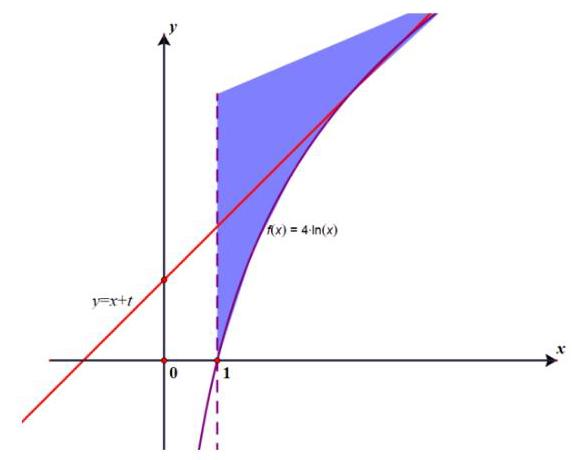
\includegraphics[max width=0.4\textwidth]{images/bo_d6dceus601uc73dvofhg_170_815_1268_572_460_0.jpg}
\end{center}
\hspace*{3em} 

依题意可得: 存在点 \(\left( {{x}_{0},{y}_{0}}\right)\) ,对阴影部分的点 \(\left( {x,y}\right)\) ,均有 \(y - x \leq  {y}_{0} - {x}_{0}\) ,

欲求 \({y}_{0} - {x}_{0}\) 的最小值,即求 \(y - x\) 的最小值.

设 \(y - x = t\) ,即 \(y = x + t\) ,找出临界情况,即直线 \(y = x + t\) 与 \(y = 4\ln x\) 相切.

设切点为 \(\left( {{x}_{1},{y}_{1}}\right)\) ,则由 \(k = \frac{4}{{x}_{1}} = 1\) 可解得 \({x}_{1} = 4\) ,此时切点为 \(\left( {4,4\ln 4}\right)\) ,代入直线方程得 \(t = 4\ln  - 4 = 8\ln 2 - 4\) ,故 \(y - x\) 的最小值为 \(8\ln 2 - 4\) ,所以 \({y}_{0} - {x}_{0} \geq  8\ln 2 - 4\)

法 2: 原题等价于 \({\left( y - x\right) }_{\max } \leq  {\left\lbrack  {\left( {y}_{0} - {x}_{0}\right) }_{\max }\right\rbrack  }_{\min }\) ,因为 \(\left( {{x}_{0},{y}_{0}}\right)  \in  {M}_{{a}_{0}}\) ,所以 \({y}_{0} = {\left( a\ln {x}_{0} + \frac{1}{a}\right) }^{2}\) ,

所以 \({y}_{0} - {x}_{0} = {\left( a\ln {x}_{0} + \frac{1}{a}\right) }^{2} - {x}_{0} \geq  {\left( 2\sqrt{\ln {x}_{0}}\right) }^{2} - {x}_{0} = 4\ln {x}_{0} - {x}_{0}\)

设 \(f\left( {x}_{0}\right)  = 4\ln {x}_{0} - {x}_{0}\) ,则 \({f}^{\prime }\left( {x}_{0}\right)  = \frac{4}{{x}_{0}} - 1 = \frac{4 - {x}_{0}}{{x}_{0}}\)

令 \({f}^{\prime }\left( {x}_{0}\right)  = \frac{4 - {x}_{0}}{{x}_{0}} > 0 \Rightarrow  {x}_{0} \in  \left( {0,4}\right) ,{f}^{\prime }\left( {x}_{0}\right)  = \frac{4 - {x}_{0}}{{x}_{0}} < 0 \Rightarrow  {x}_{0} \in  \left( {4, + \infty }\right)\)

所以 \(f\left( {x}_{0}\right)\) 在 \(\left( {0,4}\right)\) 单调递增,在 \(\left( {4, + \infty }\right)\) 单调递减; \(f{\left( {x}_{0}\right) }_{\max } = f\left( 4\right)  = 8\ln 2 - 4\)

故 \({y}_{0} - {x}_{0} \in  \lbrack 8\ln 2 - 4, + \infty ) \ll\)

3.【2025.12 普陀高三一模 12】设 \(k \in  \mathbf{R}\) ,函数 \(y = f\left( x\right)\) 和 \(y = g\left( x\right)\) 的表达式分别为 \(f\left( x\right)  = {\mathrm{e}}^{x} - {kx},g\left( x\right)  = {x}^{2} + \left( {k - 2}\right) x + \frac{1}{4}\) ,若对任意的实数 \({x}_{0}\) ,皆有 \(f\left( {x}_{0}\right)  \cdot  g\left( {x}_{0}\right)  \geq  0\) 成立, 则 \(k\) 的取值范围是\_\_\_\_\_.

【答案】 \(\left\lbrack  {1,e}\right\rbrack\)

【解析】因为 \(f\left( {x}_{0}\right)  \cdot  g\left( {x}_{0}\right)  \geq  0\) ,即 \(\left( {{e}^{{x}_{0}} - k{x}_{0}}\right)  \cdot  \left\lbrack  {{x}_{0}^{2} + \left( {k - 2}\right) {x}_{0} + \frac{1}{4}}\right\rbrack   \geq  0\) 对任意 \({x}_{0} \in  \mathbb{R}\) 恒成立. 当 \({x}_{0} = 0\) 显然成立;

当 \({x}_{0} \neq  0\) 时,

有 \(\left( {\frac{{e}^{{x}_{0}}}{{x}_{0}} - k}\right)  \cdot  \left\lbrack  {{x}_{0} + \left( {k - 2}\right)  + \frac{1}{4{x}_{0}}}\right\rbrack   \geq  0\) ,变形得 \(\left( {k - \frac{{e}^{{x}_{0}}}{{x}_{0}}}\right)  \cdot  \left\lbrack  {k - \left( {2 - {x}_{0} - \frac{1}{4{x}_{0}}}\right) }\right\rbrack   \leq  0\)  \circled{1} .

设 \(m\left( x\right)  = \frac{{e}^{x}}{x}\) ,则 \({m}^{\prime }\left( x\right)  = \frac{{e}^{x}\left( {x - 1}\right) }{{x}^{2}}\therefore\) 当 \(x \in  \left( {-\infty ,0}\right)\) 时, \({m}^{\prime }\left( x\right)  < 0,m\left( x\right)  = \frac{{e}^{x}}{x}\) 单调递减,且此时 \(m\left( x\right)  = \frac{{e}^{x}}{x}\) 的函数值均小于 0 ;

\(\therefore\) 当 \(x \in  \left( {0,1}\right)\) 时, \({m}^{\prime }\left( x\right)  < 0,m\left( x\right)  = \frac{{e}^{x}}{x}\) 单调递减;

\(\therefore\) 当 \(x \in  \left( {0, + \infty }\right)\) 时, \({m}^{\prime }\left( x\right)  > 0,m\left( x\right)  = \frac{{e}^{x}}{x}\) 单调递增;

所以 \(m{\left( x\right) }_{\text{ 极小值 }} = m\left( 1\right)  = e,m\left( x\right)  = \frac{{e}^{x}}{x}\) 的值域为 \(\left( {-\infty ,0}\right)  \cup  \lbrack e, + \infty )\) .

再设 \(n\left( x\right)  = 2 - {x}_{0} - \frac{1}{4{x}_{0}}\) ,根据耐克函数的图像及其变化规律可知: \(n\left( x\right)  = 2 - {x}_{0} - \frac{1}{4{x}_{0}}\) 的值域为 \(\left( {-\infty ,1\rbrack \cup \lbrack 3, + \infty }\right)\) . 再结合 \circled{1} 式的特点可知: 要使其任意 \({x}_{0} \in  \mathbb{R}\) 恒成立, \(k \in  \left\lbrack  {1,e}\right\rbrack\) .

【总结】本题与 2024 届虹口二模 12 题有异曲同工之之妙.

【附】(2024 届虹口二模 12)已知关于 \(x\) 的不等式 \(\left( {\ln x - {kx}}\right) \left\lbrack  {{x}^{2} - \left( {k + 3}\right) x + 4}\right\rbrack   \leq  0\) 对任意 \(x \in  \left( {0, + \infty }\right)\) 均成立，则实数 \(k\) 的取值范围为\_\_\_\_\_.

【答案】 \(\left\lbrack  {\frac{1}{e},1}\right\rbrack\)

【解析】解法一: \(\left( {\ln x - {kx}}\right) \left\lbrack  {\left( {{x}^{2} - {3x} + 4}\right)  - {kx}}\right\rbrack   \leq  0\) 原题题意转化为对任意 \(x > 0,y = {kx}\) 夹在 \(y = \ln x\) 与 \(y = {x}^{2} - {3x} + 4\) 之间.

令 \(g\left( x\right)  = {x}^{2} - {3x} + 4,f\left( x\right)  = \ln x\) 研究两函数作图。过原点分别作两函数图像的切线,设切线斜率分别为 \({k}_{1},{k}_{2}\) .

设 \(B\left( {{x}_{2},{x}_{2}^{2} - 3{x}_{2} + 4}\right) ,{k}_{1} = 2{x}_{2} - 3 = \frac{{x}_{2}^{2} - 3{x}_{2} + 4}{{x}_{2}},\because {k}_{1} > 0,\therefore {x}_{2} = 2,{k}_{1} = 1\) ; 设 \(A\left( {{x}_{1},\ln {x}_{1}}\right) ,{k}_{2} = \frac{1}{{x}_{1}} = \frac{\ln {x}_{1}}{{x}_{1}},\therefore {x}_{1} = e,{k}_{2} = \frac{1}{e}\) ,所以 \(k \in  \left\lbrack  {\frac{1}{e},1}\right\rbrack\) .

\begin{center}
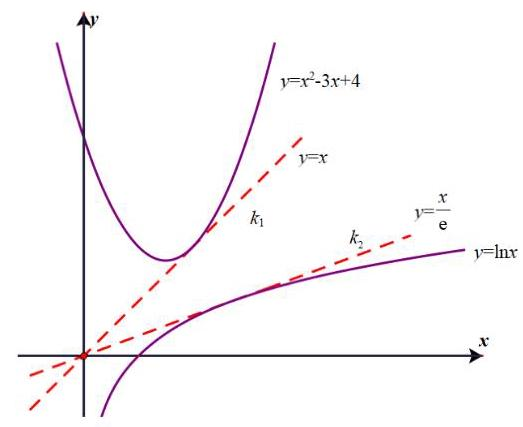
\includegraphics[max width=0.4\textwidth]{images/bo_d6dceus601uc73dvofhg_172_257_1109_523_427_0.jpg}
\end{center}
\hspace*{3em} 

\begin{center}
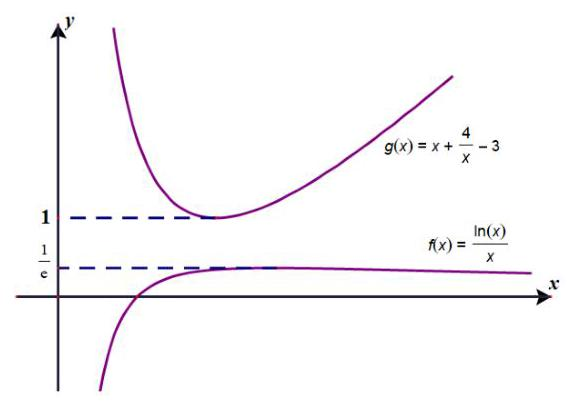
\includegraphics[max width=0.4\textwidth]{images/bo_d6dceus601uc73dvofhg_172_802_1124_568_402_0.jpg}
\end{center}
\hspace*{3em} 

解法二: 将原题题意转化为 \({x}^{2}\left( {\frac{\ln x}{x} - k}\right) \left\lbrack  {\left( {x + \frac{4}{x} - 3}\right)  - k}\right\rbrack   \leq  0\) .

\(\because {x}^{2} > 0,\therefore y = k\) 夹在 \(y = \frac{\ln x}{x}\) 与 \(y = x + \frac{4}{x} - 3\) 之间.

令 \(f\left( x\right)  = \frac{\ln x}{x},g\left( x\right)  = x + \frac{4}{x} - 3\) ,研究两函数性质,作图如下: 由图可知 \(k \in  \left\lbrack  {\frac{1}{e},1}\right\rbrack\) .

4.【2025.12 黄浦高三一模 19】在 \(\bigtriangleup  {ABC}\) 中， \(\angle {BAC} = \frac{3\pi }{4},{AB} = 6,{AC} = 3\sqrt{2}\) .

(1)求 \({BC}\) 的长和 \(\angle B\) 的正弦值；

(2)若点 \(D\) 在 \({BC}\) 边上，且 \(\angle {BAD} = \theta\) ，设 \({AD} = f\left( \theta \right)\) ，求 \(f\left( \theta \right)\) 的表达式，并判断是否存在 \({\theta }_{0}\) ,使得 \(f\left( \theta \right)\) 在 \(\theta  = {\theta }_{0}\) 处的瞬时变化率等于 \(- f\left( {\theta }_{0}\right)\) .

\begin{center}
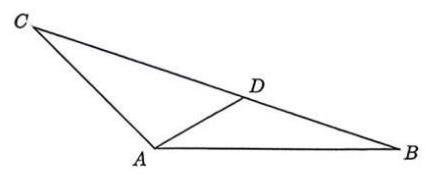
\includegraphics[max width=0.3\textwidth]{images/bo_d6dceus601uc73dvofhg_173_974_544_427_177_0.jpg}
\end{center}
\hspace*{3em} 

【答案】(1) \(3\sqrt{10},\frac{\sqrt{10}}{10}\) (2) \(f\left( \theta \right)  = \frac{6}{3\sin \theta  + \cos \theta },\theta  \in  \left\lbrack  {0,\frac{3\pi }{4}}\right\rbrack\) ，存在

【解析】(1) 在 \(\bigtriangleup {ABC}\) 中, \(B{C}^{2} = A{B}^{2} + A{C}^{2} - {2AB} \cdot  {AC}\cos \frac{3\pi }{4}\)

\(= {36} + {18} - 2 \cdot  6 \cdot  3\sqrt{2}\left( {-\frac{\sqrt{2}}{2}}\right)  = {90}\) ,故 \({BC} = 3\sqrt{10}\) . .3 分

由 \(\frac{AC}{\sin B} = \frac{BC}{\sin A}\) ,可得 \(\sin B = \frac{AC}{BC}\sin A = \frac{3\sqrt{2}}{3\sqrt{10}} \cdot  \frac{\sqrt{2}}{2} = \frac{\sqrt{10}}{10}\) . .6 分

(2)在 \(\bigtriangleup {ABD}\) 中， \(\sin \angle {ADB} = \sin \left( {\pi  - \theta  - B}\right)  = \sin \left( {\theta  + B}\right)\) ， .7 分由 \(\frac{AD}{\sin B} = \frac{AB}{\sin \left( {\theta  + B}\right) }\) ,可知 \({AD} = \frac{6\sin B}{\sin \left( {\theta  + B}\right) } = \frac{6 \cdot  \frac{\sqrt{10}}{10}}{\sin \theta  \cdot  \frac{3\sqrt{10}}{10} + \cos \theta  \cdot  \frac{\sqrt{10}}{10}} = \frac{6}{3\sin \theta  + \cos \theta }\) 故 \(f\left( \theta \right)  = \frac{6}{3\sin \theta  + \cos \theta }\left( {0 \leq  \theta  \leq  \frac{3\pi }{4}}\right)\) . .11 分 \({f}^{\prime }\left( \theta \right)  = \frac{-6\left( {3\cos \theta  - \sin \theta }\right) }{{\left( 3\sin \theta  + \cos \theta \right) }^{2}}\) ,由 \({f}^{\prime }\left( \theta \right)  =  - f\left( \theta \right)  \Leftrightarrow  3\cos \theta  - \sin \theta  = 3\sin \theta  + \cos \theta\) 且 \(\theta  \in  \left\lbrack  {0,\frac{3\pi }{4}}\right\rbrack \; \Leftrightarrow  \tan \theta  = \frac{1}{2}\) 且 \(\theta  \in  \left\lbrack  {0,\frac{3\pi }{4}}\right\rbrack   \Leftrightarrow  \theta  = \arctan \frac{1}{2} \in  \left\lbrack  {0,\frac{3\pi }{4}}\right\rbrack\) ,故存在 \({\theta }_{0}\) ,使得 \({f}^{\prime }\left( {\theta }_{0}\right)  =  - f\left( {\theta }_{0}\right)\) , 即存在 \({\theta }_{0}\) ,使得 \(f\left( \theta \right)\) 在 \(\theta  = {\theta }_{0}\) 处的瞬时变化率等于 \(- f\left( {\theta }_{0}\right)\) . .14 分

5.【2025.12 宝山高三一模 21】已知连续函数 \(y = f\left( x\right)\) 和 \(y = g\left( x\right)\) ,设 \(F\left( x\right)  = f\left( x\right)  - g\left( x\right)\) ,集合 \(M = \{ x \mid  F\left( x\right)  \geq  0\}\) .

(1)若指数函数 \(y = g\left( x\right)\) 的图像过点 \(\left( {\frac{1}{2},2}\right)\) ，且 \(f\left( x\right)  = g\left( {2x}\right)\) ，求 \(M\) ；

(2)若 \(f\left( x\right)  = {e}^{x} - a\ln x,g\left( x\right)  = a - {e}^{x}\) ，且 \(y = f\left( x\right)\) 在区间 \(\left( {0,1}\right)\) 上存在极值点 \(t\) ，求实数 \(a\) 的取值范围,并判断 \(t\) 是否属于 \(M\) ,请说明理由;

(3)若 \(y = f\left( x\right)\) 的导函数 \(y = {f}^{\prime }\left( x\right)\) 是 \(R\) 上的严格减函数， \(g\left( x\right)  = {ax} + b\left( {a,b \in  R}\right)\) ，且函数 \(y = f\left( x\right)\) 在 \(x = {x}_{0}\) 处的切线方程是 \(y = h\left( x\right)\) . 求证: " \(M = \left\{  {x}_{0}\right\}\) " 的充要条件是 " \(h\left( x\right)  = g{\left( x\right) }^{\prime \prime }\) .

【答案】(1) \(g\left( x\right)  = {4}^{x},M = \lbrack 0, + \infty )\) (2) \(a \in  \left( {0,e}\right) ,t \in  M\) (3)证明见解析

【解析】(1) 设 \(g\left( x\right)  = {a}^{x}\left( {a > 0,a \neq  1}\right)\) ,由题意可知 \(g\left( \frac{1}{2}\right)  = {a}^{\frac{1}{2}} = 2\) ,则 \(a = 4\) 所以 \(f\left( x\right)  = {4}^{2x},g\left( x\right)  = {4}^{x}\) ,由 \({4}^{2x} - {4}^{x} \geq  0\) 得 \(x \geq  0\) ,即 \(M = \{ x \mid  x \geq  0\}\) .

(2) \({f}^{\prime }\left( x\right)  = \frac{x{e}^{x} - a}{x}\) ，设 \(h\left( x\right)  = x{e}^{x} - a\left( {0 < x < 1}\right)\)

因为 \({h}^{\prime }\left( x\right)  = {e}^{x}\left( {1 + x}\right)  > 0\) ,所以 \(h\left( x\right)\) 在 \(\left( {0,1}\right)\) 上是严格增函数,所以 \(- a < h\left( x\right)  < e - a\) ,

又因为 \(y = f\left( x\right)\) 在 \(\left( {0,1}\right)\) 上存在极值点 \(t\) ,所以 \(- a\left( {e - a}\right)  < 0\) ,解得 \(0 < a < e\) .

由 \({f}^{\prime }\left( t\right)  = 0\) 得, \(t{e}^{t} - a = 0\) ,则 \({e}^{t} = \frac{a}{t}\)

所以 \(F\left( t\right)  = f\left( t\right)  - g\left( t\right)  = 2{e}^{t} - a\ln t - a = \frac{2a}{t} - a\ln t - a = \frac{a\left( {2 - t - t\ln t}\right) }{t}\) ,

因为 \(0 < a < e,0 < t < 1\) ,所以 \(2 - t - t\ln t > 0\) ,从而 \(F\left( t\right)  > 0\) ,即 \(t \in  M\) .

(3) \circled{1} 已知 \(M = \left\{  {x}_{0}\right\}\) ，则当 \(x \neq  {x}_{0}\) 时， \(F\left( x\right)  < 0\)

因为 \(y = F\left( x\right)\) 是连续函数且 \(F\left( {x}_{0}\right)  \geq  0\) ,所以 \(F\left( {x}_{0}\right)  = 0\)

所以 \({x}_{0}\) 是 \(y = F\left( x\right)\) 的一个极大值点,故 \({F}^{\prime }\left( {x}_{0}\right)  = 0\)

又 \(F\left( x\right)  = f\left( x\right)  - \left( {{ax} + b}\right)\) ,于是 \(\left\{  \begin{array}{l} f\left( {x}_{0}\right)  - \left( {a{x}_{0} + b}\right)  = 0 \\  {f}^{\prime }\left( {x}_{0}\right)  - a = 0 \end{array}\right.\)

所以 \(y = f\left( x\right)\) 在 \(x = {x}_{0}\) 处的切线方程为: \(y - f\left( {x}_{0}\right)  = {f}^{\prime }\left( {x}_{0}\right) \left( {x - {x}_{0}}\right)\)

代入化简得 \(y = {ax} + b\) ,即 \(h\left( x\right)  = g\left( x\right)\)

 \circled{2}  已知 \(h\left( x\right)  = \mathrm{g}\left( x\right)  = {ax} + b\) ，又 \(y = f\left( x\right)\) 在 \(x = {x}_{0}\) 处的切线是 \(y - f\left( {x}_{0}\right)  = {f}^{\prime }\left( {x}_{0}\right) \left( {x - {x}_{0}}\right)\) ，

即 \(h\left( x\right)  = {f}^{\prime }\left( {x}_{0}\right) x + f\left( {x}_{0}\right)  - {x}_{0}{f}^{\prime }\left( {x}_{0}\right)\) ,

所以 \(\left\{  \begin{array}{l} {f}^{\prime }\left( {x}_{0}\right)  = a \\  f\left( {x}_{0}\right)  - {x}_{0}{f}^{\prime }\left( {x}_{0}\right)  = b \end{array}\right.\) ,所以 \(\left\{  \begin{array}{l} {F}^{\prime }\left( {x}_{0}\right)  = 0 \\  F\left( {x}_{0}\right)  = 0 \end{array}\right.\) ,

因为 \({F}^{\prime }\left( x\right)  = {f}^{\prime }\left( x\right)  - a\) ,又因为 \(y = {f}^{\prime }\left( x\right)\) 是 \(\mathbf{R}\) 上的严格减函数,

所以 \(y = {F}^{\prime }\left( x\right)\) 也是 \(\mathbf{R}\) 上的严格减函数,

当 \(x > {x}_{0}\) 时, \({F}^{\prime }\left( x\right)  < {F}^{\prime }\left( {x}_{0}\right)  = 0\) ,所以 \(F\left( x\right)\) 在 \(\left( {{x}_{0}, + \infty }\right)\) 上严格减,则 \(F\left( x\right)  < F\left( {x}_{0}\right)\)

当 \(x < {x}_{0}\) 时, \({F}^{\prime }\left( x\right)  > {F}^{\prime }\left( {x}_{0}\right)  = 0\) ,所以 \(F\left( x\right)\) 在 \(\left( {-\infty ,{x}_{0}}\right)\) 上严格增,则 \(F\left( x\right)  < F\left( {x}_{0}\right)\) ,

所以 \(M = \left\{  {x \mid  F\left( x\right)  \geq  0}\right\}   = \left\{  {x}_{0}\right\}\) ,必要性成立.

综上即证. \(\ll\)

6.【2025.12 长宁高三一模 21】已知 \(a \in  \mathbf{R},f\left( x\right)  = {2x} - \ln x + a\) .

(1)求函数 \(y = f\left( x\right)\) 的驻点；

( 2 )设 \(g\left( x\right)  = \left\{  \begin{matrix} f\left( x\right) ,x > 0 \\  g\left( {x + 1}\right) ,x < 0 \end{matrix}\right.\) ，若关于 \(x\) 的方程 \(g\left( x\right)  + g\left( {-x}\right)  = 0\) 在区间 \(\left( {-1,0}\right)\) 内有解，求 \(a\) 的取值范围;

(3)定义 \(\operatorname{sgn}\left( x\right)  = \left\{  \begin{array}{l} 1,x > 0 \\  0,x = 0 \\   - 1,x < 0 \end{array}\right.\) ,设 \(h\left( x\right)  = {2x} - \left( {{2x} - f\left( x\right) }\right) \operatorname{sgn}\left( {{2x} - f\left( x\right) }\right) ,h\left( {x}_{0}\right)  = \frac{t}{a}\) ,若存在实数 \(a\) ,使得 \(\left\{  {x\left| {\;h\left( x\right)  \geq  \frac{t}{a}}\right. }\right\}   \neq  \left\lbrack  {{x}_{0}, + \infty }\right)\) ,求实数 \(t\) 的最小值.

【答案】(1) \(x = \frac{1}{2}\) (2) \(a \leq   - 1 - \ln 2\) (3) \(- \frac{2}{e}\)

【解析】(1) \({f}^{\prime }\left( x\right)  = 2 - \frac{1}{x}\) ,令 \({f}^{\prime }\left( x\right)  = 0\) ,得 \(x = \frac{1}{2}\) ,所以函数 \(y = f\left( x\right)\) 的驻点为 \(x = \frac{1}{2}\)

(2)设 \(x \in  \left( {-1,0}\right)\) ，则 \(x + 1 \in  \left( {0,1}\right) \text{ ， } - x \in  \left( {0,1}\right) \; g\left( x\right)  = g\left( {x + 1}\right)  = f\left( {x + 1}\right)  = 2\left( {x + 1}\right)  - \ln \left( {x + 1}\right)  + a,\;g\left( {-x}\right)  = f\left( {-x}\right)  = 2\left( {-x}\right)  - \ln \left( {-x}\right)  + a.\) 由 \(g\left( x\right)  + g\left( {-x}\right)  = 0\) ,得 \(2 + {2a} = \ln \left( {-{x}^{2} - x}\right)\) ,

因为 \(x \in  \left( {-1,0}\right)\) ,所以 \(- {x}^{2} - x \in  \left( {0,\frac{1}{4}}\right\rbrack  ,\ln \left( {-{x}^{2} - x}\right)  \in  \left( {-\infty ,\ln \frac{1}{4}}\right\rbrack\) ,得 \(a \leq   - 1 - \ln 2\) ,

(3) \(h\left( x\right)  = \left\{  \begin{array}{ll} {2x} - \ln x + a, & x > {e}^{a} \\  2{e}^{a}, & x = {e}^{a} \\  {2x} + \ln x - a, & 0 < x < {e}^{a} \end{array}\right.\) ,设 \(p\left( x\right)  = {2x} - \ln x + a,q\left( x\right)  = {2x} + \ln x - a\)

因为 \({p}^{\prime }\left( x\right)  = 2 - \frac{1}{x}\) ,当 \(x \in  \left( {0,\frac{1}{2}}\right)\) 时, \({p}^{\prime }\left( x\right)  < 0\) ,当 \(x \in  \left( {\frac{1}{2}, + \infty }\right)\) 时, \({p}^{\prime }\left( x\right)  > 0\)

当 \(x \in  \left( {0, + \infty }\right)\) 时, \({q}^{\prime }\left( x\right)  = 2 + \frac{1}{x} > 0\) ,

所以函数 \(y = {2x} - \ln x + a\) 在 \(\left( {0,\frac{1}{2}}\right)\) 上严格减,在 \(\left( {\frac{1}{2}, + \infty }\right)\) 上严格增

函数 \(y = {2x} + \ln x - a\) 在 \(\left( {0, + \infty }\right)\) 上严格增.

 \circled{1}  当 \({e}^{a} \geq  \frac{1}{2}\) ，即 \(a \geq  \ln \frac{1}{2}\) 时， \(y = h\left( x\right)\) 在 \(\left( {0,{e}^{a}}\right\rbrack\) 上严格增，在 \(\left\lbrack  {{e}^{a}, + \infty }\right)\) 严格增， 进而在 \(\left( {0, + \infty }\right)\) 上严格增, \(\left\{  {x\left| {\;h\left( x\right)  \geq  \frac{t}{a}}\right. }\right\}   = \left\lbrack  {{x}_{0}, + \infty }\right)\) ,不满足题意.

 \circled{2}  当 \({e}^{a} < \frac{1}{2}\) ，即 \(a < \ln \frac{1}{2}\) 时， \(y = h\left( x\right)\) 在 \(\left( {0,{e}^{a}}\right\rbrack\) 及 \(\left\lbrack  {\frac{1}{2}, + \infty }\right)\) 上严格增，在 \(\left( {{e}^{a},\frac{1}{2}}\right)\) 严格减， \(y = h\left( x\right)\) 有极大值 \(2{e}^{a}\) ,极小值 \(1 + \ln 2 + a\) .

当 \(1 + \ln 2 + a \leq  \frac{t}{a} \leq  2{e}^{a}\) 时, \(\left\{  {x\left| {\;h\left( x\right)  \geq  \frac{t}{a}}\right. }\right\}   \neq  \left\lbrack  {{x}_{0}, + \infty }\right)\) ,满足题意.

因为 \(a < \ln \frac{1}{2} < 0\) ,所以 \({2a}{e}^{a} \leq  t \leq  a\left( {a + 1 + \ln 2}\right)\) .

设 \(s\left( a\right)  = {2a}{e}^{a}\) ,则 \({s}^{\prime }\left( a\right)  = 2\left( {1 + a}\right) {e}^{a}\) ,

当 \(a \in  \left( {-\infty , - 1}\right)\) 时, \({s}^{\prime }\left( a\right)  < 0\) ,当 \(a \in  \left( {-1, + \infty }\right)\) 时, \({s}^{\prime }\left( a\right)  > 0\)

所以 \(y = s\left( a\right)\) 在 \(\left( {-\infty , - 1}\right)\) 严格减,在 \(\left( {-1, + \infty }\right)\) 严格增,得 \(s\left( a\right)  \geq  s\left( {-1}\right)  =  - \frac{2}{e}\)

因为 \(- 1 < \ln \frac{1}{2}\) ,所以当 \(a =  - 1\) 时, \(t\) 取得最小值 \(- \frac{2}{e}\) . \(\; \propto\)

7.【2025.12 松江高三一模 21】已知函数 \(y = x - 1 - a\ln x\) ，正常数 \(a \in  R\) ，记 \(y = f\left( x\right)\) .

(1)当 \(a = 1\) 时,试判断函数 \(y = f\left( x\right)\) 在区间 \(\lbrack 1, + \infty )\) 上的单调性,并说明理由;

(2)若函数 \(g\left( x\right)  = {x}^{2} - f\left( x\right)\) 既存在极小值也存在极大值，求实数 \(a\) 的取值范围；

(3)求证:对于任意正整数 \(n\) ，都有 \(1 + \frac{1}{3} + \frac{1}{5} + \cdots  + \frac{1}{{2n} + 1} > \frac{1}{2}\ln \left\lbrack  {2\left( {n + 1}\right) }\right\rbrack\) .

【答案】(1)单调递增

(2) \(\left( {0,\frac{1}{8}}\right)\) (3)证明见解析

【解析】(1)由题知 \(y = f\left( x\right)  = x - \ln x - 1,\lbrack 1, + \infty )\) ,

由题意得 \({f}^{\prime }\left( x\right)  = 1 - \frac{1}{x} = \frac{x - 1}{x} \geq  0\) 恒成立,

所以函数 \(y = f\left( x\right)\) 在区间 \(\lbrack 1, + \infty )\) 上严格增. 4 分

(2)方法一: \(g\left( x\right)  = {x}^{2} - x + 1 + a\ln x\) ，， -5 分

令 \(h\left( x\right)  = 2{x}^{2} - x + a\) ,则 \(h\left( x\right)  = 0\) 有两个不同的正解 \({x}_{1},{x}_{2}\) , -6 分

所以只需满足 \(\left\{  \begin{array}{l} \Delta  = 1 - {8a} > 0 \\  {x}_{1} + {x}_{2} = \frac{1}{2} > 0 \\  {x}_{1}{x}_{2} = \frac{a}{2} > 0 \end{array}\right.\) ,得到 \(a \in  \left( {0,\frac{1}{8}}\right)\) , -8 分

此时,当 \(x \in  \left( {0,{x}_{1}}\right)\) 时, \({g}^{\prime }\left( x\right)  > 0,\therefore y = g\left( x\right)\) 严格增.

当 \(x \in  \left( {{x}_{1},{x}_{2}}\right)\) 时, \({g}^{\prime }\left( x\right)  > 0,\therefore y = g\left( x\right)\) 严格减.

当 \(x \in  \left( {{x}_{2}, + \infty }\right)\) 时, \({g}^{\prime }\left( x\right)  > 0,\therefore y = g\left( x\right)\) 严格增.

存在极大值 \(y = g\left( {x}_{1}\right)\) 和极小值 \(y = g\left( {x}_{2}\right)\) ,综上所述, \(a \in  \left( {0,\frac{1}{8}}\right)\) , 10 分

方法二: \(g\left( x\right)  = {x}^{2} - x + 1 + a\ln x,{g}^{\prime }\left( x\right)  = {2x} - 1 + \frac{a}{x} = \frac{2{x}^{2} - x + a}{x}\) , -5 分

令 \(h\left( x\right)  = 2{x}^{2} - x + a\) ,则 \(h\left( x\right)  = 0\) 有两个不同的正解 \({x}_{1},{x}_{2}\) , -6 分

即 \(a =  - 2{x}^{2} + x\) ,当 \(x > 0\) 时有两个不同的交点,

\(a =  - 2{\left( x - \frac{1}{4}\right) }^{2} + \frac{1}{8}\) ,数形结合得 \(a \in  \left( {0,\frac{1}{8}}\right)\) , -8 分

此时,当 \(x \in  \left( {0,{x}_{1}}\right)\) 时, \({g}^{\prime }\left( x\right)  > 0,\therefore y = g\left( x\right)\) 严格增.

当 \(x \in  \left( {{x}_{1},{x}_{2}}\right)\) 时, \({g}^{\prime }\left( x\right)  < 0,\therefore y = g\left( x\right)\) 严格减.

当 \(x \in  \left( {{x}_{2}, + \infty }\right)\) 时, \({g}^{\prime }\left( x\right)  > 0,\therefore y = g\left( x\right)\) 严格增.

存在极大值 \(y = g\left( {x}_{1}\right)\) 和极小值 \(y = g\left( {x}_{2}\right)\) ,综上所述, \(a \in  \left( {0,\frac{1}{8}}\right)\) . -10 分

方法三: \(g\left( x\right)  = {x}^{2} - x + 1 + a\ln x,{g}^{\prime }\left( x\right)  = {2x} - 1 + \frac{a}{x} = \frac{2{x}^{2} - x + a}{x}\) , -5 分

令 \(h\left( x\right)  = 2{x}^{2} - x + a = 2{\left( x - \frac{1}{4}\right) }^{2} + a - \frac{1}{8}\) ,

i) 当 \(a \geq  \frac{1}{8}\) 时, \(h\left( x\right)  \geq  0,\therefore y = g\left( x\right)\) 递增,舍. -6 分

ii) 当 \(0 < a < \frac{1}{8}\) 时, \(\because h\left( 0\right)  = a > 0,h\left( \frac{1}{4}\right)  = a - \frac{1}{8} < 0,h\left( 1\right)  = a + 1 > 0\) ,

由零点存在性定理得: 存在 \({x}_{1} \in  \left( {0,\frac{1}{4}}\right) ,{x}_{2} \in  \left( {\frac{1}{4},1}\right)\) ,使得 \(g\left( {x}_{1}\right)  = g\left( {x}_{2}\right)  = 0\) , -8 分当 \(x \in  \left( {0,{x}_{1}}\right)\) 时 \({g}^{\prime }\left( x\right)  = {2x} - 1 + \frac{a}{x} = \frac{2{x}^{2} - x + a}{x},{g}^{\prime }\left( x\right)  > 0,\therefore y = g\left( x\right)\) 严格增.

当 \(x \in  \left( {{x}_{1},{x}_{2}}\right)\) 时, \({g}^{\prime }\left( x\right)  < 0,\therefore y = g\left( x\right)\) 严格减.

当 \(x \in  \left( {{x}_{2}, + \infty }\right)\) 时, \({g}^{\prime }\left( x\right)  > 0,\therefore y = g\left( x\right)\) 严格增.

存在极大值 \(y = g\left( {x}_{1}\right)\) 和极小值 \(y = g\left( {x}_{2}\right)\) ,综上所述, \(a \in  \left( {0,\frac{1}{8}}\right)\) . -10 分

(3)证明:当 \(a = 1\) 时， \(f\left( x\right)  = x - \ln x - 1\) ，

由( 1 )知， \(y = f\left( x\right)\) 在区间 \(\lbrack 1, + \infty )\) 上严格增，

所以 \(f\left( x\right)  = x - \ln x - 1 \geq  f\left( 1\right)  = 0\) ,得到 \(x - 1 \geq  \ln x\) 在 \(\lbrack 1, + \infty )\) 上成立.

所以 \(x \geq  \ln \left( {x + 1}\right)\) 在 \(\lbrack 0, + \infty )\) 上成立, 12 分

对于任意正整数 \(n\) ,令 \(x = \frac{2}{{2n} - 1}\) ,则 \(\frac{2}{{2n} - 1} \geq  \ln \left( {\frac{2}{{2n} - 1} + 1}\right)  = \ln \left( {{2n} + 1}\right)  - \ln \left( {{2n} - 1}\right)\) 14 分所以

\(2\left( {1 + \frac{1}{3} + \frac{1}{5} + \cdots  + \frac{1}{{2n} - 1} + \frac{1}{{2n} + 1}}\right)  > \ln 3 - \ln 1 + \ln 5 - \ln 3 + \ln 7 - \ln 5 + \cdots\)

\(+ \ln \left( {{2n} + 1}\right)  - \ln \left( {{2n} - 1}\right)  + \ln \left( {{2n} + 3}\right)  - \ln \left( {{2n} + 1}\right)  = \ln \left( {{2n} + 3}\right)  > \ln 2\left( {n + 1}\right)\)

即 \(1 + \frac{1}{3} + \frac{1}{5} + \cdots  + \frac{1}{{2n} + 1} > \frac{1}{2}\ln 2\left( {n + 1}\right)\) ,命题得证. -18 分类

8.【2025.12 徐汇高三一模 21】已知函数 \(y = f\left( x\right)\) 的定义域为 \(D\) ,若其导函数 \(y = {f}^{\prime }\left( x\right)\) 在 \(D\) 上是严格减函数,则称 \(f\left( x\right)\) 是一个“ \(S\) 函数”.

(1)设 \({f}_{1}\left( x\right)  = \ln x,{f}_{2}\left( x\right)  = {\mathrm{e}}^{x}\) . 分别判断 \(y = {f}_{1}\left( x\right) \text{ 、 }y = {f}_{2}\left( x\right)\) 是否为“ \(S\) 函数”，并说明理由;

(2)已知数列 \(\left\{  {b}_{n}\right\}\) 是公差为 \(d\left( {d > 0}\right)\) 的等差数列,且 \(\left\{  {b}_{n}\right\}\) 的各项都为正数,若定义在 \(\left( {0, + \infty }\right)\) 上的函数 \(y = g\left( x\right)\) 是 “ \(S\) 函数”,求证: \(g\left( {b}_{n + 3}\right)  - g\left( {b}_{n + 2}\right)  < g\left( {b}_{n + 1}\right)  - g\left( {b}_{n}\right)\) ;

(3)已知“ \(S\) 函数” \(y = F\left( x\right)\) 的定义域为 \(\mathbf{R}\) ，不等式 \(F\left( x\right)  > 0\) 的解集为 \(\left( {-\infty ,0}\right)\) . 证明:函数 \(y = F\left( x\right)\) 在 \(\mathbf{R}\) 上是严格减函数.

【答案】(1) \({f}_{1}\left( x\right)\) 是, \({f}_{2}\left( x\right)\) 不是 (2)证明见解析 (3)证明见解析

【解析】(1) \({f}_{1}^{\prime }\left( x\right)  = \frac{1}{x}\) 是 \(\left( {0, + \infty }\right)\) 上的严格减函数,故 \({f}_{1}\left( x\right)\) 是 “ \(S\) 函数”. \({f}_{2}^{\prime }\left( x\right)  = {\mathrm{e}}^{x}\) 是 \(\mathbf{R}\) 上的严格增函数,故 \({f}_{2}\left( x\right)\) 不是 “ \(S\) 函数”.

(2)证明:因为 \(y = g\left( x\right)\) 是 “ \(S\) 函数”，故 \(y = {g}^{\prime }\left( x\right)\) 在 \(\left( {0, + \infty }\right)\) 上严格减.

设 \(\left\{  {b}_{n}\right\}\) 的公差为 \(d\left( {d > 0}\right)\) ,令 \(h\left( x\right)  = g\left( {x + d}\right)  - g\left( x\right) \left( {x > 0}\right)\) .

则 \({h}^{\prime }\left( x\right)  = {g}^{\prime }\left( {x + d}\right)  - {g}^{\prime }\left( x\right)  < 0\) ,从而 \(h\left( x\right)\) 为 \(\left( {0, + \infty }\right)\) 上的严格减函数.

又 \({b}_{n + 2} > {b}_{n}\) ,因此 \(h\left( {b}_{n + 2}\right)  < h\left( {b}_{n}\right)  \Rightarrow  g\left( {{b}_{n + 2} + d}\right)  - g\left( {b}_{n + 2}\right)  < g\left( {{b}_{n} + d}\right)  - g\left( {b}_{n}\right)\) ,

即 \(g\left( {b}_{n + 3}\right)  - g\left( {b}_{n + 2}\right)  < g\left( {b}_{n + 1}\right)  - g\left( {b}_{n}\right)\) .

(3)证明:反证法. 假设存在 \({x}_{1} < {x}_{2}\) ，使得 \(F\left( {x}_{1}\right)  \leq  F\left( {x}_{2}\right)\) .

令 \(d = {x}_{2} - {x}_{1} > 0\) ,同(2)可得 \(G\left( x\right)  = F\left( {x + d}\right)  - F\left( x\right)\) 是 \(\mathbf{R}\) 上的严格减函数.

所以 \(F\left( {x}_{1}\right)  - F\left( {{x}_{1} - d}\right)  > F\left( {{x}_{1} + d}\right)  - F\left( {x}_{1}\right)  = F\left( {x}_{2}\right)  - F\left( {x}_{1}\right)  \geq  0\) .

记 \(p = F\left( {x}_{1}\right)  - F\left( {{x}_{1} - d}\right)  > 0\) ,所以对任意 \(k \in  \mathbf{N},F\left( {{x}_{1} - {kd}}\right)  - F\left( {{x}_{1} - \left( {k + 1}\right) d}\right)  \geq  p > 0\) .

累加可得, \(F\left( {x}_{1}\right)  - F\left( {{x}_{1} - {nd}}\right)  = \mathop{\sum }\limits_{{k = 1}}^{n}\left( {F\left( {{x}_{1} - \left( {k - 1}\right) d}\right)  - F\left( {{x}_{1} - {kd}}\right) }\right)  \geq  {np}\) .

即 \(F\left( {{x}_{1} - {nd}}\right)  \leq  F\left( {x}_{1}\right)  - {np}\) .

因此,当正整数 \(n > \max \left\{  {\frac{{x}_{1}}{d},\frac{F\left( {x}_{1}\right) }{p}}\right\}\) 时, \({x}_{1} - {nd} < 0\) 且 \(F\left( {{x}_{1} - {nd}}\right)  \leq  F\left( {x}_{1}\right)  - {np} < 0\) ,

与 “ \(F\left( x\right)  > 0\) 的解集为 \(\left( {-\infty ,0}\right)\) ” 矛盾. 所以 \(F\left( x\right)\) 在 \(\mathbf{R}\) 上是严格减函数. \(>\)

9.【2025.12 奉贤高三一模 21】记 \(y = {f}^{\prime }\left( x\right) ,y = {g}^{\prime }\left( x\right)\) 分别为函数 \(y = f\left( x\right)\) 和 \(y = g\left( x\right)\) 的导数,存在 \({x}_{0} \in  \mathbf{R}\) ,满足 \(f\left( {x}_{0}\right)  = g\left( {x}_{0}\right)\) 且 \({f}^{\prime }\left( {x}_{0}\right)  = {g}^{\prime }\left( {x}_{0}\right)\) ,则称 \({x}_{0}\) 为 \(y = f\left( x\right)\) 和 \(y = g\left( x\right)\) 的一个“ \(\Omega\) 点”.

(1)若函数 \(f\left( x\right)  = a{x}^{2} - 1\) 与 \(g\left( x\right)  = \ln x\) 存在 “ \(\Omega\) 点”，求实数 \(a\) 的值；

(2)证明函数 \(f\left( x\right)  = \sin x\) 与 \(g\left( x\right)  = {x}^{2} + {2x} - 2\) 不存在 “ \(\Omega\) 点”；

(3)已知函数 \(f\left( x\right)  =  - {x}^{2} + a,g\left( x\right)  = \frac{b{\mathrm{e}}^{x}}{x}\) ，对任意的 \(a > 0\) ，判断是否存在 \(b > 0\) ，使得函数 \(y = f\left( x\right)\) 和 \(y = g\left( x\right)\) 在区间 \(\left( {0, + \infty }\right)\) 内存在 “ \(\Omega\) 点”,请说明理由.

【答案】( 1 ) \(a = \frac{e}{2}\) (2)证明见解析 (3)存在

【解析】(1) \(\left\{  \begin{matrix} a{x}^{2} - 1 = \ln x \\  {2ax} = \frac{1}{x} \end{matrix}\right.\) 在 \(\left( {0, + \infty }\right)\) 上有解,将得 \(a = \frac{1}{2{x}^{2}} = \frac{e}{2}\) .

( 2 )假设 \(f\left( x\right)  = \sin x\) 与 \(g\left( x\right)  = {x}^{2} + {2x} - 2\) 存在 “ \(\Omega\) 点”,则 \(\left\{  \begin{matrix} \sin x = {x}^{2} + {2x} - 2 \\  \cos x = {2x} + 2 \end{matrix}\right.\) 有解.

由 \(\cos x \in  \left\lbrack  {-1,1}\right\rbrack\) 得 \({2x} + 2 \in  \left\lbrack  {-1,1}\right\rbrack\) ,即 \(x \in  \left\lbrack  {-\frac{3}{2}, - \frac{1}{2}}\right\rbrack\)

由 \(\sin x \in  \left\lbrack  {-1,1}\right\rbrack\) 得 \({x}^{2} + {2x} - 2 \in  \left\lbrack  {-1,1}\right\rbrack\) ,即 \(x \in  \left\lbrack  {-3, - \sqrt{2} - 1}\right\rbrack   \cup  \left\lbrack  {\sqrt{2} - 1,1}\right\rbrack\)

而 \(\left\lbrack  {-\frac{3}{2}, - \frac{1}{2}}\right\rbrack   \cap  \left( {\left\lbrack  {-3, - \sqrt{2} - 1}\right\rbrack   \cup  \left\lbrack  {\sqrt{2} - 1,1}\right\rbrack  }\right)  = \varnothing\)

所以假设不成立,即 \(f\left( x\right)  = \sin x\) 与 \(g\left( x\right)  = {x}^{2} + {2x} - 2\) 不存在 “ \(\Omega\) 点”.

(3) \(\left\{  {\begin{matrix}  - {x}^{2} + a = \frac{b{e}^{x}}{x} \\   - {2x} = \frac{b{e}^{x}\left( {x - 1}\right) }{{x}^{2}} \end{matrix},x \in  \left( {0, + \infty }\right) }\right.\)

将 \(b{e}^{x} = \left( {-{x}^{2} + a}\right) x\) 代入 \(- {2x} = \frac{b{e}^{x}\left( {x - 1}\right) }{{x}^{2}}\) ,得 \({x}^{3} - 3{x}^{2} - {ax} + a = 0\)

令 \(H\left( x\right)  = {x}^{3} - 3{x}^{2} - {ax} + a\) ,则 \(H\left( 0\right)  = a > 0,H\left( \sqrt{a}\right)  =  - {2a} < 0\)

由零点存在定理得,存在 \({x}_{0} \in  \left( {0,\sqrt{a}}\right)\) ,使得 \(H\left( {x}_{0}\right)  = 0\) . 此时 \(b{e}^{{x}_{0}} = \left( {-{x}_{0}{}^{2} + a}\right) {x}_{0} > 0\) ,

则存在 \(b = \left( {-{x}_{0}{}^{2} + a}\right) {x}_{0}{e}^{-{x}_{0}} > 0\) ,使得 \(y = f\left( x\right)\) 与 \(y = g\left( x\right)\) 在 \(\left( {0, + \infty }\right)\) 上存在 “ \(\Omega\) 点”.

10.【2025.12 崇明高三一模 21】已知函数 \(y = f\left( x\right) ,x \in  D\) ,其导函数是 \(y = {f}^{\prime }\left( x\right)\) . 对于任意 \(t \in  D\) ,记曲线 \(y = f\left( x\right)\) 在点 \(P\left( {t,f\left( t\right) }\right)\) 处的切线方程为 \(y = {l}_{t}\left( x\right)\) . 定义集合 \(M\left( {f,t}\right)  = \left\{  {x \mid  f\left( x\right)  \leq  {l}_{t}\left( x\right) ,x \in  D}\right\}  .\)

(1)若 \(f\left( x\right)  = {x}^{3} - 2{x}^{2} + x\) ，求集合 \(M\left( {f,1}\right)\) ；

(2)若定义域 \(D = \mathbf{R}\) 且函数 \(y = f\left( x\right)\) 是偶函数，证明:若 \({x}_{0} \in  M\left( {f,t}\right)\) 则 \(- {x}_{0} \in  M\left( {f, - t}\right)\) ；

(3)设 \(f\left( x\right)  = a\ln x + \frac{1}{2}{x}^{2}\left( {a < 1}\right)\) ，若集合 \(M\left( {f,1}\right)  = \{ 1\}\) ，求实数 \(a\) 的取值范围.

【答案】(1) \(M\left( {f,1}\right)  = \{ x \mid  x = 1\) 或 \(x \leq  0\}\) (2)证明见解析 (3) \(( - \infty ,0\rbrack\)

【解析】(1) \({f}^{\prime }\left( x\right)  = 3{x}^{2} - {4x} + 1\) ,所以 \({f}^{\prime }\left( 1\right)  = 0,{l}_{t}\left( x\right)  = 0\) 2 分

由 \(f\left( x\right)  \leq  {l}_{t}\left( x\right)\) ,得: \({x}^{3} - 2{x}^{2} + x \leq  0\) ,解得 \(x = 1\) 或 \(x \leq  0\)

所以 \(M\left( {f,1}\right)  = \{ x \mid  x = 1\) 或 \(x \leq  0\}\) .4 分

(2)因为函数 \(y = f\left( x\right)\) 是偶函数，所以 \(f\left( {-x}\right)  = f\left( x\right)\) ，

所以 \({\left\lbrack  f\left( -x\right) \right\rbrack  }^{\prime } = {\left\lbrack  f\left( x\right) \right\rbrack  }^{\prime }\) ,故 \(- {f}^{\prime }\left( {-x}\right)  = {f}^{\prime }\left( x\right)\) .2 分

所以 \({l}_{t}\left( x\right)  = {f}^{\prime }\left( t\right) \left( {x - t}\right)  + f\left( t\right)\) ,

\({l}_{-t}\left( x\right)  = {f}^{\prime }\left( {-t}\right) \left( {x + t}\right)  + f\left( {-t}\right)  =  - {f}^{\prime }\left( t\right) \left( {x + t}\right)  + f\left( t\right)\) .4 分

当 \({x}_{0} \in  M\left( {f,t}\right)\) 时,有 \(f\left( {x}_{0}\right)  \leq  {f}^{\prime }\left( t\right) \left( {{x}_{0} - t}\right)  + f\left( t\right)\) ,

所以 \(f\left( {-{x}_{0}}\right)  \leq  {f}^{\prime }\left( t\right) \left( {-{x}_{0} - t}\right)  + f\left( t\right)  =  - {f}^{\prime }\left( t\right) \left( {{x}_{0} + t}\right)  + f\left( t\right)  = {l}_{-t}\left( x\right)\) ,

即 \(- {x}_{0} \in  M\left( {f, - t}\right)\) .6 分

(3)函数 \(y = f\left( x\right)\) 定义域为 \(\left( {0, + \infty }\right) ,{f}^{\prime }\left( x\right)  = \frac{a}{x} + x,{f}^{\prime }\left( 1\right)  = a + 1\) 所以 \({l}_{1}\left( x\right)  = \left( {a + 1}\right) x - a - \frac{1}{2}\)

由题意,不等式 \(f\left( x\right)  \leq  {l}_{1}\left( x\right)\) 在区间 \(\left( {0, + \infty }\right)\) 上有且只有唯一解 \(x = 1\)

令 \(g\left( x\right)  = f\left( x\right)  - {l}_{1}\left( x\right)  = a\ln x + \frac{1}{2}{x}^{2} - \left\lbrack  {\left( {a + 1}\right) x - a - \frac{1}{2}}\right\rbrack\) ,

则不等式 \(g\left( x\right)  \leq  0\) 区间 \(\left( {0, + \infty }\right)\) 上有且只有唯一解 \(x = 1\) 3 分

\({g}^{\prime }\left( x\right)  = \left( {\frac{a}{x} + x}\right)  - \left( {a + 1}\right)  = \frac{\left( {x - 1}\right) \left( {x - a}\right) }{x}\)

\(a \leq  0\) 时, \circled{1}  当 \(0 < x < 1\) 时, \({g}^{\prime }\left( x\right)  < 0\) ,函数 \(y = g\left( x\right)\) 严格减

 \circled{2}  当 \(x > 1\) 时， \({g}^{\prime }\left( x\right)  > 0\) ，函数 \(y = g\left( x\right)\) 严格增，所以 \(M\left( {f,1}\right)  = \{ 1\}\) .5 分

\(0 < a < 1\) 时，函数 \(y = g\left( x\right)\) 在区间 \(\left( {0,a}\right)\) 上严格增，在区间 \(\left( {a,1}\right)\) 上严格减，在 \(\left( {1, + \infty }\right)\) 上严格增，

而当正数 \(x\) 趋向于 0 时, \(g\left( x\right)\) 趋向于 \(- \infty\) ,故必存在 \({x}_{0} \in  \left( {0,a}\right)\) 使得 \(g\left( x\right)  < 0\) ,

此时 \({x}_{0} \in  M\left( {f,1}\right)\) ,与题意不符

综上所述， \(a \leq  0\) .8 分

\section*{11.3 新定义综合}

1.【2025.12 黄浦高三一模 21】已知函数 \(y = f\left( x\right)\) 的定义域为 \(D\) ,对于给定实数 \(t\) ,定义集合 \({V}_{f\left( t\right) } = \left\{  {x \mid  f\left( {x + t}\right)  \geq  f\left( x\right) }\right\}  .\)

(1)若 \(f\left( x\right)  = {x}^{3} - {13x}\) ，求 \({V}_{f\left( 2\right) }\) ；

(2)若 \(D = \mathbf{R}\) ，求证: “ \(y = f\left( x\right)\) 为周期函数”的充要条件是 “存在非零常数 \(t\) ，使得 \({V}_{f\left( t\right) } = {V}_{f\left( {-t}\right) } = D\) ”.

(3)若 \(f\left( x\right)  = \frac{1}{2}a{\left( x - \frac{\mathrm{e}}{\mathrm{e} - 1}\right) }^{2} - x\left( {\ln x - \frac{\mathrm{e}}{\mathrm{e} - 1}}\right) ,D = \left( {0, + \infty }\right)\) ,且对于任意的 \(t \in  D\) ,都有 \({V}_{f\left( t\right) } = D\) , 求实数 \(a\) 的取值范围.

【答案】(1) \({V}_{f\left( 2\right) } = \left( {-\infty , - 3\rbrack \cup \lbrack 1, + \infty }\right)\) (2)证明见解析

(3) \(a \in  \left\lbrack  {\frac{1}{e},1}\right\rbrack\)

【解析】(1) \(f\left( {x + 2}\right)  \geq  f\left( x\right)\) ,即 \({\left( x + 2\right) }^{3} - {13}\left( {x + 2}\right)  \geq  {x}^{3} - {13x}\) ,可得 \({x}^{2} + {2x} - 3 \geq  0\) , 解得 \(x \geq  1\) 或 \(x \leq   - 3\) . 故 \({V}_{f\left( 2\right) } = \left( {-\infty , - 3\rbrack \cup \lbrack 1, + \infty }\right)\) . .4 分

(2)若 \(D = \mathrm{R}\) 且 \(y = f\left( x\right)\) 为周期函数，则存在非零常数 \(t\) ，使得 \(f\left( {x + t}\right)  = f\left( x\right)\) 对一切 \(x \in  \mathrm{R}\) 恒成立,故 \(f\left( {x + t}\right)  \geq  f\left( x\right)\) 对一切 \(x \in  \mathrm{R}\) 恒成立,所以 \({V}_{f\left( t\right) } = \mathrm{R} = D\) ;

由 \(f\left( {x + t}\right)  = f\left( x\right)\) ,即 \(f\left( {x + t}\right)  = f\left( {x + t - t}\right)\) 对一切 \(x \in  \mathrm{R}\) 恒成立,可知 \(f\left( x\right)  = f\left( {x - t}\right)\) 对一切 \(x \in  \mathrm{R}\) 恒成立,故 \(f\left( {x - t}\right)  \geq  f\left( x\right)\) 对一切 \(x \in  \mathrm{R}\) 恒成立,所以 \({V}_{f\left( {-t}\right) } = \mathrm{R} = D\) .

故存在非零实数 \(t\) ,使得 \({V}_{f\left( t\right) } = {V}_{f\left( {-t}\right) } = D\) . .7 分

若 \(D = \mathrm{R}\) 且存在非零实数 \(t\) ,使得 \({V}_{f\left( t\right) } = {V}_{f\left( {-t}\right) } = D\) ,则对一切 \(x \in  \mathrm{R}\) ,都有 \(f\left( {x + t}\right)  \geq  f\left( x\right)\) 与 \(f\left( {x - t}\right)  \geq  f\left( x\right)\) 恒成立,可知对一切 \(x \in  \mathrm{R},f\left( {x + t}\right)  \geq  f\left( x\right)\) 与 \(f\left( x\right)  \geq  f\left( {x + t}\right)\) 恒成立,

从而 \(f\left( {x + t}\right)  = f\left( x\right)\) 恒成立,所以 \(y = f\left( x\right)\) 为周期函数.

综上可知: 若 \(D = \mathrm{R},\) “ \(y = f\left( x\right)\) 为周期函数”的充要条件是 “存在非零常数 \(t\) ,使得 \({V}_{f\left( t\right) } = {V}_{f\left( {-t}\right) } = {D}^{* * }.\) .10 分

(3)由 \(D = \left( {0, + \infty }\right)\) ，且对任意 \(t \in  D\) ， \({V}_{f\left( t\right) } = D\) ，可知对任意的 \(t > 0,x > 0\) ，都有 \(f\left( {x + t}\right) \; \geq  f\left( x\right)\) ,它等价于 \(y = f\left( x\right)\) 在 \(\left( {0, + \infty }\right)\) 上是增函数,

故 \({f}^{\prime }\left( x\right)  = a\left( {x - \frac{\mathrm{e}}{\mathrm{e} - 1}}\right)  - \left( {\ln x - \frac{1}{\mathrm{e} - 1}}\right)  \geq  0\) 对于 \(x \in  \left( {0, + \infty }\right)\) 恒成立, .13 分

即 \(\ln x \leq  a\left( {x - \frac{\mathrm{e}}{\mathrm{e} - 1}}\right)  + \frac{1}{\mathrm{e} - 1}\) 对于 \(x \in  \left( {0, + \infty }\right)\) 恒成立,

又直线 \(l : y = a\left( {x - \frac{\mathrm{e}}{\mathrm{e} - 1}}\right)  + \frac{1}{\mathrm{e} - 1}\) 过定点 \(A\left( {\frac{\mathrm{e}}{\mathrm{e} - 1},\frac{1}{\mathrm{e} - 1}}\right) ,y = \ln x\) 的图像在 \(x = t\) 处的切线方程为 \(y - \ln t = \frac{1}{t}\left( {x - t}\right)\) ,

若此切线过点 \(A\) ,则有 \(\frac{1}{\mathrm{e} - 1} - \ln t = \frac{1}{t}\left( {\frac{\mathrm{e}}{\mathrm{e} - 1} - t}\right)\) ,即 \(\frac{\mathrm{e}}{\mathrm{e} - 1} - \ln t = \frac{1}{t} \cdot  \frac{\mathrm{e}}{\mathrm{e} - 1}( *\)

当 \(t = 1\) 与 \(\mathrm{e}\) 时, \(\left( *\right)\) 成立,故当 \(a = 1,\frac{1}{\mathrm{e}}\) 时,直线 \(l\) 与 \(y = \ln x\) 的图像相切,

由图像可知 \(a \in  \left\lbrack  {\frac{1}{\mathrm{e}},1}\right\rbrack\) . .17 分

若 \(a \in  \left( {\frac{1}{\mathrm{e}},1}\right)\) ,则 \({f}^{\prime }\left( x\right)  > 0\) ,故 \(y = f\left( x\right)\) 在 \(\left( {0, + \infty }\right)\) 上严格增;

若 \(a = \frac{1}{\mathrm{e}}\) ,则当 \(x = \mathrm{e}\) 时, \({f}^{\prime }\left( x\right)  = 0\) ,

当 \(x \in  \left( {0,\mathrm{e}}\right)  \cup  \left( {\mathrm{e}, + \infty }\right)\) 时, \({f}^{\prime }\left( x\right)  > 0\) ,此时 \(y = f\left( x\right)\) 在 \(\left( {0, + \infty }\right)\) 上严格增;

若 \(a = 1\) ,则当 \(x = 1\) 时, \({f}^{\prime }\left( x\right)  = 0\) ,

当 \(x \in  \left( {0,1}\right)  \cup  \left( {1, + \infty }\right)\) 时, \({f}^{\prime }\left( x\right)  > 0\) ,此时 \(y = f\left( x\right)\) 在 \(\left( {0, + \infty }\right)\) 上严格增.

所以当 \(a \in  \left\lbrack  {\frac{1}{\mathrm{e}},1}\right\rbrack\) 时 \(y = f\left( x\right)\) 在 \(\left( {0, + \infty }\right)\) 上必为增函数.

综上可知,所求 \(a\) 的取值范围是 \(\left\lbrack  {\frac{1}{\mathrm{e}},1}\right\rbrack\) . .18 分

\begin{center}
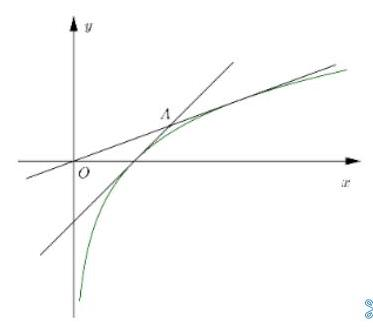
\includegraphics[max width=0.3\textwidth]{images/bo_d6dceus601uc73dvofhg_183_1009_1351_373_327_0.jpg}
\end{center}
\hspace*{3em} 

2.【2025.12 闵行高三一模 21】已知函数 \(y = f\left( x\right)\) 的定义域为 \(\mathbf{R}\) ,对于 \({x}_{0} \in  \mathbf{R}\) ,若 \(\left\{  {x \mid  f\left( x\right)  \leq  f\left( {x}_{0}\right) }\right\}   = \left( {-\infty ,{x}_{0}}\right\rbrack\) ,且 \(\left\{  {x \mid  f\left( x\right)  \geq  f\left( {x}_{0}\right) }\right\}   = \left\lbrack  {{x}_{0}, + \infty }\right)\) ,则称 \({x}_{0}\) 为 \(y = f\left( x\right)\) 的一个“ \(M\) 点”, 记 \({M}_{f}\) 为 \(y = f\left( x\right)\) 的所有“ \(M\) 点”构成的集合.

(1)若 \(f\left( x\right)  = \left\{  \begin{array}{l} 0,x = 0, \\  \frac{1}{x},x \neq  0, \end{array}\right.\) 分别判断 \(0 \in  {M}_{f}\) 与 \(1 \in  {M}_{f}\) 是否正确;

(2)证明: “ \({x}_{0} \in  {M}_{f}\) ”的一个充要条件为 “当 \(x \neq  {x}_{0}\) 时， \(\frac{f\left( x\right)  - f\left( {x}_{0}\right) }{x - {x}_{0}} > 0\) ”；

(3)已知 \(f\left( x\right)  = \left( {a - 1}\right) \left| {x - b}\right|  + \left( {a + 1}\right) \left| {x + b}\right|\) ， \(g\left( x\right)  = a{x}^{4} + 2{x}^{3} - 3\left( {b + 1}\right) {x}^{2} + {6bx} + {2b}\) ，其中 \(a\text{ 、 }b \in  \mathbf{R}\) ,记 \(A = \left\{  {y \mid  y = f\left( {x}_{0}\right) ,{x}_{0} \in  {M}_{f}}\right\}   \neq  \varnothing ,\;B = \left\{  {y \mid  y = g\left( {x}_{0}\right) ,{x}_{0} \in  {M}_{g}}\right\}   \neq  \mathbf{R}\) . 若 \(A \cap  B = A\) ,求 \(a + b\) 的取值范围.

【答案】( 1 ) \(0 \in  {M}_{f}\) 正确； \(1 \in  {M}_{f}\) 不正确. (2)证明见解析

(3) \(\left\lbrack  {\frac{1}{3},1}\right)  \cup  (1,3\rbrack\)

【解析】(1) \(f\left( x\right)  \leq  f\left( 0\right)  \Rightarrow  x \in  ( - \infty ,0\rbrack ,f\left( x\right)  \geq  f\left( 0\right)  \Rightarrow  x \in  \lbrack 0, + \infty )\) ,所以 \(0 \in  {M}_{f}\) 正确; \(f\left( x\right)  \leq  f\left( 1\right)  \Rightarrow  x \in  \left( {-\infty ,0\rbrack \cup \lbrack 1, + \infty }\right)\) ,所以 \(1 \in  {M}_{f}\) 不正确.

(2)证明:(充分性)

由 \(x \neq  {x}_{0}\) 时, \(\frac{f\left( x\right)  - f\left( {x}_{0}\right) }{x - {x}_{0}} > 0\) ,

当 \(x < {x}_{0}\) 时, \(f\left( x\right)  < f\left( {x}_{0}\right)\) ,当 \(x > {x}_{0}\) 时, \(f\left( x\right)  > f\left( {x}_{0}\right)\) .

故 \(\left\{  {x \mid  f\left( x\right)  \leq  f\left( {x}_{0}\right) }\right\}   = \left( {-\infty ,{x}_{0}}\right\rbrack\) ,且 \(\left\{  {x \mid  f\left( x\right)  \geq  f\left( {x}_{0}\right) }\right\}   = \left\lbrack  {{x}_{0}, + \infty }\right)\) ,所以 \({x}_{0} \in  {M}_{f}\) .

(必要性) 首先证明若 \({x}_{0} \in  {M}_{f}\) ,则 \(f\left( x\right)  = f\left( {x}_{0}\right)\) 有唯一解. 显然 \({x}_{0}\) 是 \(f\left( x\right)  = f\left( {x}_{0}\right)\) 的一个解, 若 \(f\left( x\right)  = f\left( {x}_{0}\right)\) 还存在另一解 \({x}_{0}{}^{\prime }\) ,且 \({x}_{0}{}^{\prime } \neq  {x}_{0}\) .

当 \({x}_{0}{}^{\prime } > {x}_{0}\) 时, \(\left\{  {x \mid  f\left( x\right)  \leq  f\left( {x}_{0}\right) }\right\}   = \left( {-\infty ,{x}_{0}}\right\rbrack   \cup  \left\{  {x}_{0}^{\prime }\right\}\) ,矛盾;

当 \({x}_{0}{}^{\prime } < {x}_{0}\) 时, \(\left\{  {x \mid  f\left( x\right)  \geq  f\left( {x}_{0}\right) }\right\}   = \left\lbrack  {{x}_{0}, + \infty }\right)  \cup  \left\{  {x}_{0}\right\}\) ,矛盾; 故 \(f\left( x\right)  = f\left( {x}_{0}\right)\) 有唯一解.

其次,若 \({x}_{0} \in  {M}_{f}\) ,则 \(\left\{  {x \mid  f\left( x\right)  < f\left( {x}_{0}\right) }\right\}   = \left( {-\infty ,{x}_{0}}\right)\) ,且 \(\left\{  {x \mid  f\left( x\right)  > f\left( {x}_{0}\right) }\right\}   = \left( {{x}_{0}, + \infty }\right)\) ,

所以当 \(x < {x}_{0}\) 时, \(f\left( x\right)  < f\left( {x}_{0}\right) ,\frac{f\left( x\right)  - f\left( {x}_{0}\right) }{x - {x}_{0}} > 0\) ;

当 \(x > {x}_{0}\) 时, \(f\left( x\right)  > f\left( {x}_{0}\right) ,\frac{f\left( x\right)  - f\left( {x}_{0}\right) }{x - {x}_{0}} > 0\) . 故当 \(x \neq  {x}_{0}\) 时, \(\frac{f\left( x\right)  - f\left( {x}_{0}\right) }{x - {x}_{0}} > 0\) .

(3)对于 \(f\left( x\right)  = \left( {a - 1}\right) \left| {x - b}\right|  + \left( {a + 1}\right) \left| {x + b}\right|\)

若 \(b > 0\) ,则:

 \circled{1}  当 \(a > 0\) 时,若 \(x \in  ( - \infty , - b\rbrack\) ,则 \(f\left( x\right)  =  - {2ax} - {2b}\) ,因此 \(y = f\left( x\right)\) 在 \(( - \infty , - b\rbrack\) 上是严格减函数; 对任意实数 \({x}_{0}\) ,取 \({x}_{1} \in  \left( {-\infty ,{x}_{0}}\right)  \cap  \left( {-\infty ,\frac{-{2b} - f\left( {x}_{0}\right) }{2a}}\right)\) ,则 \(\frac{f\left( {x}_{1}\right)  - f\left( {x}_{0}\right) }{{x}_{1} - {x}_{0}} < 0\) ,

由( 2 )知， \({x}_{0}\) 不是 \(y = f\left( x\right)\) 的 \(M\) 点，故函数 \(y = f\left( x\right)\) 不存在 \(\mathrm{M}\) 点；

 \circled{2}  当 \(a < 0\) 时,若 \(x \in  \lbrack b, + \infty )\) ,则 \(f\left( x\right)  = {2ax} + {2b}\) ,同理可得函数 \(y = f\left( x\right)\) 不存在 \(\mathrm{M}\) 点;

 \circled{3}  当 \(a = 0\) 时, \(f\left( x\right)  = \left\{  \begin{array}{l}  - {2b},\text{ 当 }x \leq   - b \\  {2x},\text{ 当 } - b < x < b \\  {2b},\text{ 当 }x \geq  b \end{array}\right.\) ,此时 \(A = \left( {-{2b},{2b}}\right)\) .

若 \(b < 0\) ,则:

 \circled{1}  当 \(a > 0\) 时,若 \(x \in  ( - \infty , - b\rbrack\) ,则 \(f\left( x\right)  =  - {2ax} - {2b}\) ,同理得函数 \(y = f\left( x\right)\) 不存在 \(\mathrm{M}\) 点;

 \circled{2}  当 \(a < 0\) 时,若 \(x \in  \lbrack b, + \infty )\) ,则 \(f\left( x\right)  = {2ax} + {2b}\) ,同理得函数 \(y = f\left( x\right)\) 不存在 \(\mathrm{M}\) 点;

 \circled{3}  当 \(a = 0\) 时, \(f\left( x\right)  = \left\{  \begin{array}{l}  - {2b},\text{ 当 }x \leq  b \\   - {2x},\text{ 当 }b < x <  - b \\  {2b},\text{ 当 }x \geq   - b \end{array}\right.\) ,函数 \(y = f\left( x\right)\) 不存在 \(\mathrm{M}\) 点.

若 \(b = 0\) ,则 \(f\left( x\right)  = {2a}\left| x\right|\) 不存在 \(\mathrm{M}\) 点. 从而可得 \(a = 0,b > 0,A = \left( {-{2b},{2b}}\right)\) .

对于 \(g\left( x\right)  = a{x}^{4} + 2{x}^{3} - 3\left( {b + 1}\right) {x}^{2} + {6bx} + {2b} = 2{x}^{3} - 3\left( {b + 1}\right) {x}^{2} + {6bx} + {2b}\) ,

\({g}^{\prime }\left( x\right)  = 6{x}^{2} - 6\left( {b + 1}\right) x + {6b} = 6\left( {x - 1}\right) \left( {x - b}\right)\) ,令 \({g}^{\prime }\left( x\right)  = 0,x = 1\) 或 \(x = b\) ,

 \circled{1}  当 \(b = 1\) 时， \({g}^{\prime }\left( x\right)  = 6{\left( x - 1\right) }^{2} \geq  0,B = R\) ，矛盾，所以 \(b \neq  1\) ；

 \circled{2}  当 \(b > 1\) 时， \(g\left( x\right)\) 在 \(\left( {-\infty ,1}\right)\) 严格增，在 \(\left( {1,b}\right)\) 严格减，在 \(\left( {b, + \infty }\right)\) 严格增，

所以 \(B = \left( {-\infty ,g\left( b\right) }\right)  \cup  \left( {g\left( 1\right) , + \infty }\right)\)

由 \(A \cap  B = A,g\left( b\right)  = 2{b}^{3} - 3\left( {b + 1}\right) {b}^{2} + 6{b}^{2} + {2b} \geq  {2b}\) ,解之得 \(1 < b \leq  3\) ;

 \circled{3}  当 \(0 < b < 1\) 时， \(g\left( x\right)\) 在 \(\left( {-\infty ,b}\right)\) 单调递增，在 \(\left( {b,1}\right)\) 单调递减，在 \(\left( {1, + \infty }\right)\) 单调递增，

同理, \(g\left( 1\right)  = 2 - 3\left( {b + 1}\right)  + {6b} + {2b} \geq  {2b}\) ,解得 \(\frac{1}{3} \leq  b < 1\) .

综上所述: \(a + b \in  \left\lbrack  {\frac{1}{3},1}\right)  \cup  (1,3\rbrack\) . \(\ll\)

3.【2025.12 杨浦高三一模 21】已知区间 \(I \subseteq  R\) ，函数 \(y = f\left( x\right)\) 的定义域为 \(I\) ,若函数 \(y = f\left( x\right)\) 满足: 对任意 \({x}_{1},{x}_{2} \in  I\) ,均有 \(\left| {f\left( {x}_{1}\right)  - f\left( {x}_{2}\right) }\right|  \leq  \left| {{x}_{1} - {x}_{2}}\right|\) ,则称函数 \(y = f\left( x\right)\) 为压缩函数.

(1)判断函数 \(f\left( x\right)  = {x}^{2},x \in  \left\lbrack  {-\frac{1}{2},\frac{1}{2}}\right\rbrack\) 是否为压缩函数？并说明理由;

(2)若函数 \(f\left( x\right)  = {e}^{x} + {kx},x \in  \left\lbrack  {0,1}\right\rbrack\) 为压缩函数，求实数 \(k\) 的取值范围；

(3)已知函数 \(y = f\left( x\right) ,x \in  I\) 为压缩函数，求证: \(y = f\left( x\right) ,x \in  I\) 为单调函数的充要条件是: 对任意 \({x}_{1},{x}_{2} \in  I\) ,均有 \(\left( {f\left( {x}_{1}\right)  - f\left( \frac{{x}_{1} + {x}_{2}}{2}\right) }\right)  \cdot  \left( {f\left( {x}_{2}\right)  - f\left( \frac{{x}_{1} + {x}_{2}}{2}\right) }\right)  \leq  0\) .

【答案】(1)是压缩函数，理由见解析 (2) \(\left\lbrack  {-2,1 - e}\right\rbrack\) (3)证明见解析

【解析】(1) 函数 \(f\left( x\right)  = {x}^{2}\left( {x \in  \left\lbrack  {-\frac{1}{2},\frac{1}{2}}\right\rbrack  }\right)\) 是压缩函数,2 分

理由: 对任意 \({x}_{1},{x}_{2} \in  \left\lbrack  {-\frac{1}{2},\frac{1}{2}}\right\rbrack\) ,易知 \(- 1 \leq  {x}_{1} + {x}_{2} \leq  1\)

所以 \(\left| {f\left( {x}_{1}\right)  - f\left( {x}_{2}\right) }\right|  = \left| {{x}_{1}^{2} - {x}_{2}^{2}}\right|  = \left| {{x}_{1} + {x}_{2}}\right| \left| {{x}_{1} - {x}_{2}}\right|  \leq  \left| {{x}_{1} - {x}_{2}}\right|\) ,4 分

(2)由题意， \(\forall {x}_{1},{x}_{2} \in  \left\lbrack  {0,1}\right\rbrack\) ，都有 \(\left| {f\left( {x}_{1}\right)  - f\left( {x}_{2}\right) }\right|  \leq  \left| {{x}_{1} - {x}_{2}}\right|\) . 显然，当 \({x}_{1} = {x}_{2}\) 时，符合.

不妨设 \({x}_{1} > {x}_{2}\) ,则 \(\left| {f\left( {x}_{1}\right)  - f\left( {x}_{2}\right) }\right|  \leq  {x}_{1} - {x}_{2}\) ,即 \({x}_{2} - {x}_{1} \leq  f\left( {x}_{1}\right)  - f\left( {x}_{2}\right)  \leq  {x}_{1} - {x}_{2}\) .

设 \(g\left( x\right)  = f\left( x\right)  - x\) ,在 \(x \in  \left\lbrack  {0,1}\right\rbrack\) 上为减函数, \(h\left( x\right)  = f\left( x\right)  + x\) ,在 \(x \in  \left\lbrack  {0,1}\right\rbrack\) 上为增函数.

\(g\left( x\right)  = {e}^{x} + \left( {k - 1}\right) x,{g}^{\prime }\left( x\right)  = {e}^{x} + \left( {k - 1}\right)  \leq  0,\forall x \in  \left\lbrack  {0,1}\right\rbrack  .\)

所以 \(- k + 1 \geq  {\left( {e}^{x}\right) }_{\max } = e\) ,即 \(k \leq  1 - e\) .

\(h\left( x\right)  = {e}^{x} + \left( {k + 1}\right) x,{h}^{\prime }\left( x\right)  = {e}^{x} + \left( {k + 1}\right)  \geq  0,\forall x \in  \left\lbrack  {0,1}\right\rbrack  .\)

所以 \(- k - 1 \leq  {\left( {e}^{x}\right) }_{\min } = 1\) ,即 \(k \geq   - 2\) . 所以 \(\mathrm{k}\) 的取值范围是 \(\left\lbrack  {-2,1 - e}\right\rbrack\)

(3)证明:必要性:已知 \(y = f\left( x\right) \left( {x \in  I}\right)\) 为单调函数，不妨设 \(y = f\left( x\right)\) 在 \(I\) 上为增函数任取 \({x}_{1},{x}_{2} \in  I\) ,不妨设 \({x}_{1} \leq  {x}_{2}\) ,则 \({x}_{1} \leq  \frac{{x}_{1} + {x}_{2}}{2} \leq  {x}_{2}\) ,

由 \(y = f\left( x\right) \left( {x \in  I}\right)\) 为增函数,所以 \(f\left( {x}_{1}\right)  \leq  f\left( \frac{{x}_{1} + {x}_{2}}{2}\right)  \leq  f\left( {x}_{2}\right)\) ,

进而 \(\left( {f\left( {x}_{1}\right)  - f\left( \frac{{x}_{1} + {x}_{2}}{2}\right) }\right)  \cdot  \left( {f\left( {x}_{2}\right)  - f\left( \frac{{x}_{1} + {x}_{2}}{2}\right) }\right)  \leq  0;\) 12 分

充分性: 已知任意 \({x}_{1},{x}_{2} \in  I\) ,均有 \(\left( {f\left( {x}_{1}\right)  - f\left( \frac{{x}_{1} + {x}_{2}}{2}\right) }\right)  \cdot  \left( {f\left( {x}_{2}\right)  - f\left( \frac{{x}_{1} + {x}_{2}}{2}\right) }\right)  \leq  0\) 假设 \(y = f\left( x\right) \left( {x \in  I}\right)\) 不为单调函数,

则存在 \(a,b,c \in  I,a < b < c\) ,使得 \(f\left( a\right)  < f\left( b\right)  > f\left( c\right)\) 或 \(f\left( a\right)  > f\left( b\right)  < f\left( c\right)\) ,

不妨设 \(f\left( a\right)  < f\left( b\right)  > f\left( c\right)\) ,取实数 \({\lambda }_{1} < {\lambda }_{2}\) 满足 \(f\left( a\right) ,f\left( c\right)  < {\lambda }_{1},f\left( b\right)  > {\lambda }_{2}\)

记 \({I}_{1} = \left\lbrack  {{a}_{1},{c}_{1}}\right\rbrack   = \left\lbrack  {a,c}\right\rbrack\) ,由于 \(\left( {f\left( a\right)  - f\left( \frac{a + c}{2}\right) }\right) \left( {f\left( c\right)  - f\left( \frac{a + c}{2}\right) }\right)  \leq  0\)

可知: \(f\left( \frac{a + c}{2}\right)  < {\lambda }_{1}\) ,所以 \(\frac{a + c}{2} \neq  b\) ,

若 \(\frac{a + c}{2} < b\) ,记 \({I}_{2} = \left\lbrack  {{a}_{2},{c}_{2}}\right\rbrack   = \left\lbrack  {a,\frac{a + c}{2}}\right\rbrack\) ,否则记 \({I}_{2} = \left\lbrack  {{a}_{2},{c}_{2}}\right\rbrack   = \left\lbrack  {\frac{a + c}{2},c}\right\rbrack\)

重复上面的操作,可以得到区间 \({I}_{n} = \left\lbrack  {{a}_{n},{c}_{n}}\right\rbrack\) 满足: \({a}_{n} < b < {c}_{n}\) ,

对任意 \(n \in  {N}^{ * }\) . 且区间 \({I}_{n}\) 的长度 \({l}_{n} = {c}_{n} - {a}_{n} = \frac{1}{{2}^{n - 1}}\left( {c - a}\right) ,f\left( {a}_{n}\right) ,f\left( {c}_{n}\right)  < {\lambda }_{1}\) .

因为函数 \(y = f\left( x\right) \left( {x \in  I}\right)\) 为压缩函数可得:

\(\left| {f\left( b\right)  - f\left( {a}_{n}\right) }\right|  \leq  \left| {b - {a}_{n}}\right|  \leq  \left| {{c}_{n} - {a}_{n}}\right|  = \frac{1}{{2}^{n - 1}}\left( {c - a}\right) ,\)

又 \(\left| {f\left( b\right)  - f\left( {a}_{n}\right) }\right|  = f\left( b\right)  - f\left( {a}_{n}\right)  > {\lambda }_{2} - {\lambda }_{1}\) ,

记 \(\lambda  = {\lambda }_{2} - {\lambda }_{1} > 0\) ,所以 \(\lambda  < \frac{1}{{2}^{n - 1}}\left( {c - a}\right)\) 对任意 \(n \in  {N}^{ * }\) 恒成立.

取 \({n}_{0} > 1 + {\log }_{2}\left( \frac{c - a}{\lambda }\right) ,{n}_{0} \in  {N}^{ * }\) ,则 \(\lambda  > \frac{1}{{2}^{{n}_{0} - 1}}\left( {c - a}\right)\) ,矛盾!

所以 \(y = f\left( x\right) \left( {x \in  I}\right)\) 为单调函数. 18 分

4.【2025.12 青浦高三一模 21】已知函数 \(y = f\left( x\right)\) 定义域为 \(\mathbf{R}\) ,对于实数 \(a\) ,定义集合 \({R}_{a} = \{ x \mid  x \geq  a,f\left( x\right)  \geq  f\left( a\right) \} ,\;{L}_{a} = \{ x \mid  x \leq  a,f\left( x\right)  \geq  f\left( a\right) \} .\)

(1)若 \(f\left( x\right)  = {x}^{2}\) ，求 \({R}_{1}\) 和 \({L}_{1}\) ；

(2)给定实数 \(a\) ，若 \(f\left( x\right)  = {x}^{2}\left( {x - 3}\right)\) 满足对任意 \(b > a\) ，均有 \({R}_{b} \subseteq  {R}_{a}\) ，求 \(a\) 的取值范围；

(3)若集合 \(A\text{ 、 }B\) 满足: \(x \in  A \Leftrightarrow   - x \in  B\) ，则称 \(A\) 和 \(B\) 互为对称集. 证明: “函数 \(y = f\left( x\right)\) 为偶函数”的充要条件是“对任意实数 \(a,{R}_{a}\) 与 \({L}_{-a}\) 互为对称集”.

【答案】(1) \({R}_{1} = \lbrack 1, + \infty ),\;{L}_{1} = ( - \infty , - 1\rbrack \bigcup \{ 1\}\) (2) \(\left( {-\infty , - 1\rbrack \cup \lbrack 2, + \infty }\right)\) (3)见解析

【解析】(1) \({R}_{1} = \lbrack 1, + \infty ),{L}_{1} = ( - \infty , - 1\rbrack  \cup  \{ 1\}\)

(2)首先，由 \(b \in  {R}_{b}\) 知 \(b \in  {R}_{a},\therefore f\left( b\right)  \geq  f\left( a\right)\) . 其次，当 \(f\left( b\right)  \geq  f\left( a\right)\) 时，由 \(x \geq  b,f\left( x\right)  \geq  f\left( b\right)\) 可以推得 \(x \geq  a,f\left( x\right)  \geq  f\left( a\right) ,\therefore {R}_{b} \subseteq  {R}_{a}\) . 因此只需保证对任意 \(b > a\) ,均有 \(f\left( b\right)  \geq  f\left( a\right)\) . \({f}^{\prime }\left( x\right)  = {3x}\left( {x - 2}\right)\) ,令 \({f}^{\prime }\left( x\right)  = 0\) 得 \(x = 0\) 或 2 .

在 \(\left( {-\infty ,0}\right)\) 和 \(\left( {2, + \infty }\right)\) 上, \({f}^{\prime }\left( x\right)  > 0,f\left( x\right)\) 严格增; 在 \(\left( {0,2}\right)\) 上, \({f}^{\prime }\left( x\right)  < 0,f\left( x\right)\) 严格减.

\(x = 2\) 时, \(f\left( x\right)\) 取得极小值 \(f\left( 2\right)  =  - 4\) ,且方程 \(f\left( x\right)  = {x}^{2}\left( {x - 3}\right)  =  - 4\) 即 \({\left( x - 2\right) }^{2}\left( {x + 1}\right)  = 0\) 的另一个根为 -1 . 结合图像可知, \(a\) 的取值范围是 \(\left( {-\infty , - 1\rbrack \cup \lbrack 2, + \infty }\right)\)

\begin{center}
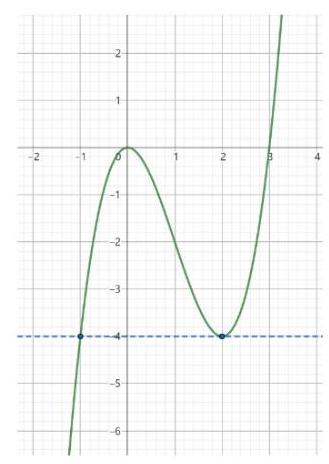
\includegraphics[max width=0.2\textwidth]{images/bo_d6dceus601uc73dvofhg_188_1078_766_329_464_0.jpg}
\end{center}
\hspace*{3em} 

(3) 必要性.

若函数 \(y = f\left( x\right)\) 为偶函数,则对任意实数 \(a\) ,

\(x \in  {R}_{a} \Leftrightarrow  x \geq  a\) 且 \(f\left( x\right)  \geq  f\left( a\right)  \Leftrightarrow   - x \leq   - a\) 且 \(f\left( {-x}\right)  \geq  f\left( {-a}\right)  \Leftrightarrow   - x \in  {L}_{-a}\) ,

所以 \({R}_{a}\) 与 \({L}_{-a}\) 互为对称集.

充分性.

若对任意实数 \(a,{R}_{a}\) 与 \({L}_{-a}\) 互为对称集. 下面证明对任意 \(t > 0,f\left( t\right)  = f\left( {-t}\right)\) . 假设 \(f\left( t\right)  \neq  f\left( {-t}\right)\) ,

 \circled{1} 若 \(f\left( t\right)  > f\left( {-t}\right)\) ，则 \(t \in  {R}_{-t}\) ，则 \(- t \in  {L}_{t}\) ， \(\therefore f\left( {-t}\right)  \geq  f\left( t\right)\) ，矛盾；

 \circled{2} 若 \(f\left( t\right)  < f\left( {-t}\right)\) ，则 \(- t \in  {L}_{t}\) ，则 \(t \in  {R}_{-t}\) ， \(\therefore f\left( t\right)  \geq  f\left( {-t}\right)\) ，矛盾.

\(\therefore\) 假设不成立. \(\therefore\) 对任意 \(t > 0,f\left( t\right)  = f\left( {-t}\right) .\therefore\) 函数 \(y = f\left( x\right)\) 为偶函数.

5.【2025.12 普陀高三一模 21】设函数 \(y = f\left( x\right)\) 的定义域为 \(D\) ,导函数为 \(y = {f}^{\prime }\left( x\right)\) ,对于实数 \(t\) ,若存在 \({x}_{0} \in  D\) ,使得 \(f\left( {t{x}_{0}}\right)  = t{f}^{\prime }\left( {x}_{0}\right)\) 成立,则称函数 \(y = f\left( x\right)\) 具有性质 \(P\left( t\right)\) .

(1)若函数 \(f\left( x\right)  = \ln x\) ，请判断该函数是否具有性质 \(P\left( 1\right)\) ，并说明理由；

(2)设 \(a \in  \mathrm{R}\) ，若函数 \(f\left( x\right)  = {x}^{3} + a\) 具有性质 \(P\left( 2\right)\) ，且 \({x}_{0}\) 的值恰有三个，求 \(a\) 的取值范围；

(3)若函数 \(f\left( x\right)  = {\mathrm{e}}^{x} + x\) ，求证:该函数具有性质 \(P\left( t\right)\) 的充要条件是 \(t > 0\) .

【答案】(1)具有

(2) \(\left( {0,\frac{1}{2}}\right)\) (3)证明见解析

【解析】(1) 由 \(f\left( x\right)  = \ln x\) 得, \({f}^{\prime }\left( x\right)  = \frac{1}{x}\)

设 \(g\left( x\right)  = f\left( x\right)  - {f}^{\prime }\left( x\right)  = \ln x - \frac{1}{x},x > 0\) ,当 \(x > 0\) 时, \({g}^{\prime }\left( x\right)  = \frac{1}{x} + \frac{1}{{x}^{2}} > 0\) , .2 分

又 \(g\left( 1\right)  = \ln 1 - \frac{1}{1} =  - 1 < 0,g\left( \mathrm{e}\right)  = \ln \mathrm{e} - \frac{1}{\mathrm{e}} = 1 - \frac{1}{\mathrm{e}} > 0\) ,则存在 \({x}_{0} \in  \left( {1,\mathrm{e}}\right)\) ,使得 \(g\left( {x}_{0}\right)  = 0\) ,

即 \(f\left( {x}_{0}\right)  = {f}^{\prime }\left( {x}_{0}\right)\) ,故函数 \(f\left( x\right)  = \ln x\) 具有性质 \(P\left( 1\right)\) .4 分

(2)由 \(f\left( x\right)  = {x}^{3} + a\) 得， \({f}^{\prime }\left( x\right)  = 3{x}^{2}\) ，

因为函数 \(f\left( x\right)  = {x}^{3} + a\) 具有性质 \(P\left( 2\right)\) ,所以存在实数 \({x}_{0}\) ,使得 \(f\left( {2{x}_{0}}\right)  = 2{f}^{\prime }\left( {x}_{0}\right)\) ,

即 \({\left( 2{x}_{0}\right) }^{3} + a = 2\left( {3{x}_{0}^{2}}\right)\) ,即 \(a =  - 8{x}_{0}^{3} + 6{x}_{0}^{2}\) , .2 分

设 \(g\left( x\right)  =  - 8{x}^{3} + 6{x}^{2}\) ,则 \({g}^{\prime }\left( x\right)  =  - {24}{x}^{2} + {12x} =  - {12x}\left( {{2x} - 1}\right)\) ,

令 \({g}^{\prime }\left( x\right)  = 0\) ,解得 \(x = 0\) 或 \(x = \frac{1}{2}\) ,列表如下:

\begin{center}
\adjustbox{max width=\textwidth}{
\begin{tabular}{|c|c|c|c|c|c|}
\hline
\(x\) & \(\left( {-\infty ,0}\right)\) & 0 & \(\left( {0,\frac{1}{2}}\right)\) & 1 2 & \(\left( {\frac{1}{2}, + \infty }\right)\) \\
\cline{1-6}
\({f}^{\prime }\left( x\right)\) & - & 0 & + & 0 & - \\
\cline{1-6}
\(f\left( x\right)\) & ↘ & 极小值 0 & ↗ & 极大值 \(\frac{1}{2}\) & ↘ \\
\cline{1-6}
\hline
\end{tabular}
}
\end{center}

.......4 分

因为函数 \(f\left( x\right)  = {x}^{3} + a\) 具有性质 \(P\left( 2\right)\) 时, \({x}_{0}\) 的值恰有三个,

所以满足条件的 \(a\) 的取值范围是 \(\left( {0,\frac{1}{2}}\right)\) . .6 分

(3)由 \(f\left( x\right)  = {\mathrm{e}}^{x} + x\) 得， \({f}^{\prime }\left( x\right)  = {\mathrm{e}}^{x} + 1\) ，

由 \(f\left( {tx}\right)  = t{f}^{\prime }\left( x\right)\) 得, \({\mathrm{e}}^{tx} + {tx} = t\left( {{\mathrm{e}}^{x} + 1}\right)\) ,设 \(g\left( x\right)  = {\mathrm{e}}^{tx} - t{\mathrm{e}}^{x} + t\left( {x - 1}\right)\) ,

先证充分性: 当 \(t > 0\) 时, \(g\left( 1\right)  = {\mathrm{e}}^{t} - t\mathrm{e}\) ,

考虑函数 \(y = {\mathrm{e}}^{x} - x\mathrm{e}\) ,则 \({y}^{\prime } = {\mathrm{e}}^{x} - \mathrm{e}\) ,

当 \(0 < x < 1\) 时， \({y}^{\prime } < 0\) ；当 \(x = 1\) 时， \({y}^{\prime } = 0\) ；当 \(x > 1\) 时， \({y}^{\prime } > 0\) ，

则函数 \(y = {\mathrm{e}}^{x} - x\mathrm{e}\) 在 \(\left( {0,1}\right)\) 上是严格减函数，在 \(\left( {1, + \infty }\right)\) 上是严格增函数，在 \(x = 1\) 时取得极小值 0,

因此,当 \(t = 1\) 时, \(g\left( 1\right)  = {\mathrm{e}}^{t} - t\mathrm{e} = 0\) ,函数 \(f\left( x\right)\) 具有性质 \(P\left( 1\right)\) ; .2 分

当 \(t > 0\) 且 \(t \neq  1\) 时, \(g\left( 1\right)  = {\mathrm{e}}^{t} - t\mathrm{e} > {\mathrm{e}}^{1} - 1 \cdot  \mathrm{e} = 0\) ,

且当 \(x \rightarrow   - \infty\) 时, \({\mathrm{e}}^{tx} \rightarrow  0, - {\mathrm{e}}^{x} \rightarrow  0,t\left( {x - 1}\right)  \rightarrow   - \infty\) ,则 \(g\left( x\right)  \rightarrow   - \infty\) ,

则存在 \({x}_{0} \in  \left( {-\infty ,1}\right)\) 满足 \(g\left( {x}_{0}\right)  = 0\) ,即 \(f\left( {t{x}_{0}}\right)  = t{f}^{\prime }\left( {x}_{0}\right)\) 成立,

则函数 \(f\left( x\right)  = {\mathrm{e}}^{x} + x\) 具有性质 \(P\left( t\right)\) . .4 分

再证必要性: 即证若函数 \(f\left( x\right)  = {\mathrm{e}}^{x} + x\) 具有性质 \(P\left( t\right)\) ,则 \(t > 0\) .

由 \(g\left( x\right)  = {\mathrm{e}}^{tx} - t{\mathrm{e}}^{x} + t\left( {x - 1}\right)\) 得, \({g}^{\prime }\left( x\right)  = t\left( {{\mathrm{e}}^{tx} - {\mathrm{e}}^{x} + 1}\right)\) ,

若 \(t = 0\) ,则 \(g\left( x\right)  = 1\) ,与已知矛盾;

若 \(t < 0\) ,设 \(h\left( x\right)  = {\mathrm{e}}^{tx} - {\mathrm{e}}^{x} + 1\) ,则 \({h}^{\prime }\left( x\right)  = t{\mathrm{e}}^{tx} - {\mathrm{e}}^{x} < 0\) ,

即函数 \(h\left( x\right)\) 是严格减函数，则函数 \({g}^{\prime }\left( x\right)\) 是严格增函数，

又 \({g}^{\prime }\left( 0\right)  = t\left( {{\mathrm{e}}^{0} - {\mathrm{e}}^{0} + 1}\right)  = t < 0,{g}^{\prime }\left( 1\right)  = t\left( {{\mathrm{e}}^{t} - \mathrm{e} + 1}\right)  > t\left( {2 - \mathrm{e}}\right)  > 0\) ,

则存在 \(m \in  \left( {0,1}\right)\) 使得 \({g}^{\prime }\left( m\right)  = 0\) ,即 \({\mathrm{e}}^{tm} - {\mathrm{e}}^{m} + 1 = 0\) ,

当 \(x \in  \left( {-\infty ,m}\right)\) 时, \({g}^{\prime }\left( x\right)  < 0\) ,即函数 \(g\left( x\right)\) 是严格减函数;

当 \(x \in  \left( {m, + \infty }\right)\) 时, \({g}^{\prime }\left( x\right)  > 0\) ,即函数 \(g\left( x\right)\) 是严格增函数.

则 \(g\left( x\right)  \geq  g\left( m\right)  = {\mathrm{e}}^{tm} - t{\mathrm{e}}^{m} + t\left( {m - 1}\right)  = \left( {1 - t}\right) {\mathrm{e}}^{m} + t\left( {m - 1}\right)  - 1\) , .6 分

需证 \({\mathrm{e}}^{m} \geq  m + 1\) ,令 \(y = {\mathrm{e}}^{x} - x - 1,x \in  \left( {0,1}\right)\) ,则 \({y}^{\prime } = {\mathrm{e}}^{x} - 1 > 0\) ,

即 \(y = {\mathrm{e}}^{x} - x - 1 > {\mathrm{e}}^{0} - 1 = 0\) .

则 \(g\left( x\right)  \geq  g\left( m\right)  \geq  \left( {1 - t}\right) \left( {m + 1}\right)  + t\left( {m - 1}\right)  - 1 = m - {2t} > 0\) ,

则不存在 \({x}_{0} \in  D\) ,使得 \(f\left( {t{x}_{0}}\right)  = t{f}^{\prime }\left( {x}_{0}\right)\) 成立,与 \(y = f\left( x\right)\) 具有性质 \(P\left( t\right)\) 矛盾.

综上所述,函数 \(f\left( x\right)\) 具有性质 \(P\left( t\right)\) 的充要条件是 \(t > 0\) . .8 分。

\section*{第十二章 复数}

\section*{【知识梳理】}

1. 什么是复数的平方根?

我们知道,实数若满足 \({x}^{2} = y\) ,则称 \(x\) 是 \(y\) 的平方根, \(y\) 的平方根是 \(\pm  x\)

同样,复数 \(a + {bi}\) 和 \(c + {di}\left( {a,b,c,d \in  R}\right)\) ,若满足 \({\left( a + bi\right) }^{2} = c + {di}\) ,则称 \(a + {bi}\) 是 \(c + {di}\) 的平方根, 因为 \({\left\lbrack  \pm \left( a + bi\right) \right\rbrack  }^{2} = c + {di}\) ,所以 \(c + {di}\) 的平方根是 \(\pm  \left( {a + {bi}}\right)\) 两个数

2. 如何求复数 \(c + {di}\) 们平方根? (其中 \(c\text{ 、 }d\) 为已知)

由 \({\left( a + bi\right) }^{2} = c + {di}\) 展开, \({a}^{2} - {b}^{2} + {2abi} = c + {di}\) ,得 \(\left\{  \begin{matrix} {a}^{2} - {b}^{2} = c \\  {2ab} = d \end{matrix}\right.\) ,解此方程即可求出 \(a.b\) ,从而得到平方根

3. 如何在复数范围内解实系数一无一次方程? 给定 \(a{x}^{2} + {bx} + c = 0\left( {a,b,c \in  R,a \neq  0}\right)\) , \(\Delta  = {b}^{2} - {4ac}\) ;

(1)当 \(\Delta  = {b}^{2} - {4ac} > 0\) 时,方程有两不等实根, \(x = \frac{-b \pm  \sqrt{{b}^{2} - {4ac}}}{2a}\) ;

(2) 当 \(\Delta  = {b}^{2} - {4ac} = 0\) 时,方程有两相等实根, \(x =  - \frac{b}{2a}\) ;

(3) 当 \(\Delta  = {b}^{2} - {4ac} < 0\) 时,方程有两共轭虚根, \(x = \frac{-b \pm  \sqrt{{4ac} - {b}^{2}}i}{2a}\)

4.复数集中实系数一元一次方程根的性质

(1)根有三种情况:两不等实根.两相等实根.一组共轭虚根.

(2)韦达定理始终成立.

5.实系数二次三项式在复数范围内的因式分解.

若 \({x}_{1}\text{ 、 }{x}_{2}\) 是 方 程 \(a{x}^{2} + {bx} + c = 0\) 的两个 根 \(\left( {a,b,c \in  R,a \neq  0}\right)\) ,则 有 \(a{x}^{2} + {bx} + c = a\left( {x - {x}_{1}}\right) \left( {x - {x}_{2}}\right)\) ,这样就可以利用实系数一完二次方程的求根公式在复数范围内作因式分解.

6.1 的立方根: \(1, - \frac{1}{2} + \frac{\sqrt{3}}{2}i, - \frac{1}{2} - \frac{\sqrt{3}}{2}i\) (可由 \({x}^{3} = 1 \Rightarrow  {x}^{3} - 1 = 0 \Rightarrow  \left( {x - 1}\right) \left( {{x}^{2} + x + 1}\right)  = 0\) 解得) 7. 令 \(\omega  =  - \frac{1}{2} + \frac{\sqrt{3}}{2}i\) ,则 \(\overline{\omega } =  - \frac{1}{2} - \frac{\sqrt{3}}{2}i\) ,由此可知:

(1)1 的立方根为 \(1,\omega ,\overline{\omega }\) ；

(2) \({\omega }^{2} + \omega  + 1 = 0,{\omega }^{3} = 1,{\omega }^{2} = \overline{\omega } = \frac{1}{\omega }\) ;

(3) \(\omega ,\overline{\omega }\) 是方程 \({x}^{2} + x + 1 = 0\) 的两根;

(4) \({\omega }^{n}\left( {n \in  {N}^{ * }}\right)\) 具有周期性: \({\omega }^{2} =  - \frac{1}{2} + \frac{\sqrt{3}}{2}i,{\omega }^{2} =  - \frac{1}{2} - \frac{\sqrt{3}}{2}i,{\omega }^{3} = 1\) ,

注:周期为 3,每三个连续相加为 0

1.【2025.12 徐汇高三一模 1】设复数 \(z = 2 + \mathrm{i}\) (其中 \(\mathrm{i}\) 为虚数单位)，则 \(\left| z\right|  =\) \_\_\_\_\_.

【答案】 \(\left| z\right|  = \sqrt{5}\) .

2.【 2025.12 闵行高三一模 3】若虚数 \(z\) 的实部为 1，虚部为正数，且 \(\left| z\right|  = \sqrt{2}\) ，则 \(z =\) \_\_\_\_\_.

【答案】 \(z = 1 + i\) .

【解析】因为虚数 \(z\) 的实部为 1,虚部为正数,且 \(\left| z\right|  = \sqrt{2}\) ,所以 \(z = 1 + i >\)

3.【2025.12 普陀高三一模 3】若复数 \(z\) 是纯虚数，且 \(\left| z\right|  = 1\) ，则 \(\frac{1}{1 - z}\) 的实部为\_\_\_\_\_.

【答案】 \(\frac{1}{2}\)

【解析】依题意可得 \(z =  \pm  i\) ,当 \(z = i\) 时, \(\frac{1}{1 - z} = \frac{1}{1 - i} = \frac{1 + i}{2}\) ,实部为 \(\frac{1}{2}\) ;

当 \(z =  - i\) 时, \(\frac{1}{1 - z} = \frac{1}{1 + i} = \frac{1 - i}{2}\) ,实部也是 \(\frac{1}{2}\) ; 综上所述: \(\frac{1}{1 - z}\) 的实部为 \(\frac{1}{2}\) .

4.【 2025.12 嘉定高三一模 3】已知复数 \(z = \frac{3 - {4i}}{4 + {3i}}\left( {i\text{ 为虚数单位 }}\right)\) ，则 \(\left| z\right|  =\) \_\_\_\_\_.

【答案】1

【解析】由 \(z = \frac{3 - 4\mathrm{i}}{4 + 3\mathrm{i}}\) 得 \(\left| z\right|  = \left| \frac{3 - 4\mathrm{i}}{4 + 3\mathrm{i}}\right|  = \frac{\left| 3 - 4\mathrm{i}\right| }{\left| 4 + 3\mathrm{i}\right| } = \frac{5}{5} = 1\) .

5.【2025.12 青浦高三一模 3】若复数 \(z = \frac{3 - 5\mathrm{i}}{1 - \mathrm{i}}\) ，则 \(\left| z\right|  =\) \_\_\_\_\_.

【答案】 \(\sqrt{17}\)

【解析】 \(\left| z\right|  = \left| \frac{3 - 5\mathrm{i}}{1 - \mathrm{i}}\right|  = \frac{\left| 3 - 5\mathrm{i}\right| }{\left| 1 - \mathrm{i}\right| } = \frac{\sqrt{34}}{\sqrt{2}} = \sqrt{17}\) .

6.【2025.12 金山高三一模 3】若复数 \(z\) 满足 \(z \cdot  i = \frac{2}{1 + i}\) ，则 \(\left| z\right|  =\)

【答案】 \(\sqrt{2}\)

【解析】依题意可得 \(z = \frac{2}{\left( {1 + i}\right) i} = \frac{2}{i - 1},\therefore \left| z\right|  = \left| \frac{2}{i - 1}\right|  = \frac{2}{\left| i - 1\right| } = \sqrt{2}\) .

7.【2025.12 杨浦高三一模 4】若复数 \(z\) 满足: \(\frac{z}{i} = 1 - {2i}\) ，则 \(\left| z\right|  =\) \_\_\_\_\_.

答案: \(\sqrt{5}\)

【解析】易得 \(z = i\left( {1 - {2i}}\right) ,\therefore \left| z\right|  = \left| i\right|  \cdot  \left| {1 - {2i}}\right|  = \sqrt{5}\) .

8.【2025.12 黄浦高三一模 4】已知 \(i\) 是虚数单位，则 \(\frac{5i}{2 - i} =\) \_\_\_\_\_.

【答案】 \(\frac{32\pi }{3}\)

【解析】化简得 \(\frac{5i}{2 - i} = \frac{{5i}\left( {2 + i}\right) }{\left( {2 - i}\right) \left( {2 + i}\right) } =  - 1 + {2i}\) .

9.【2025.12 静安高三一模 4】已知复数 \(z\) 满足 \(\left( {3 - i}\right)  \cdot  z = 3 + i\) (其中 \(\mathrm{i}\) 为虚数单位)，则复数 \(z =\) \_\_\_\_\_.

【答案】 \(\frac{4}{5} + \frac{3}{5}i\)

【解析】依题意可得: \(z = \frac{3 + i}{3 - i} = \frac{{\left( 3 + i\right) }^{2}}{\left( {3 - i}\right) \left( {3 + i}\right) } = \frac{8 + {6i}}{10} = \frac{4}{5} + \frac{3}{5}i\)

10.【2025.12 松江高三一模 4】复数 \(z = \frac{1 + {3i}}{1 + i}\) (其中 \(i\) 是虚数单位)在复平面内对应点的坐标为\_\_\_\_\_.

【答案】 \(\left( {2,1}\right)\)

【解析】化简得 \(z = \frac{1 + {3i}}{1 + i} = \frac{\left( {1 + {3i}}\right) \left( {1 - i}\right) }{\left( {1 + i}\right) \left( {1 - i}\right) } = 2 + i\) ,对应的点为 \(\left( {2,1}\right) . \ll\)

11.【2025.12 虹口高三一模 6】已知复数 \(z\) 是实系数一元二次方程 \({x}^{2} + {bx} + 2 = 0\) 的一个虚数根，则 \(\left| \bar{z}\right|  =\)

【答案】 \(\sqrt{2}\)

【解析】依题意可得: \(z \cdot  \bar{z} = 2 = {\left| \bar{z}\right| }^{2},\therefore \left| \bar{z}\right|  = \sqrt{2}\) .

12.【2025.12 奉贤高三一模 9】若复数 \(z\) 满足 \(\left| z\right|  = \sqrt{5}\) ， \(\left| {z - 1}\right|  = \left| {\operatorname{Re}z + 1}\right|\) ，则复数 \(z =\) \_\_\_\_\_.

【答案】 \(z = 1 \pm  {2i}\)

【解析】可设 \(z = a + {bi},\therefore \left| z\right|  = \sqrt{{a}^{2} + {b}^{2}} = \sqrt{5}\) ,同时 \(\sqrt{{\left( a - 1\right) }^{2} + {b}^{2}} = \left| {a + 1}\right|\) ,解得 \(\left\{  \begin{array}{l} a = 1 \\  b =  \pm  2 \end{array}\right. \; \left( {a =  - 5\text{ 舍 }}\right) ,\therefore z = 1 \pm  {2i}\) . \(\leq\)

13.【2025.12 浦东高三一模 10】已知复数 \({z}_{1}\text{ 、 }{z}_{2}\) 是实系数一元二次方程的两个根，若 \({z}_{1} = \mathrm{i}{z}_{2}\) , 则 \(\left| {{z}_{1} - \mathrm{i}}\right|\) 的最小值为\_\_\_\_\_.

【答案】 \(\frac{\sqrt{2}}{2}\)

【解析】可设 \({z}_{1} = a + {bi}\left( {a,b \in  \mathbb{R}}\right) ,\therefore {z}_{2} = a - {bi}\left( {a,b \in  \mathbb{R}}\right)\) ,由 \({z}_{1} = i{z}_{2}\) 得 \(a + {bi} = \left( {a - {bi}}\right) i\) ,化简得 \(a = b,\therefore {z}_{1} = a + {ai}\) 在复平面上对应的动点轨迹为直线 \(y = x\) ,

\(\therefore \left| {{z}_{1} - i}\right|\) 表示直线 \(y = x\) 上的动点与定点 \(\left( {0,1}\right)\) 之间的距离,

故其最小值为定点 \(\left( {0,1}\right)\) 到直线 \(y = x\) 的距离: \(d = \frac{\sqrt{2}}{2}\) .

14.【2025.12 长宁高三一模 10】在复平面上,复数 2 和 \(2\mathrm{i}\) 所对应的点分别 \(A,B\) ,复数 \({z}_{1}\) 所对应的点在线段 \({AB}\) 上移动,若 \(\left| {{z}_{1} - {z}_{2}}\right|  = 1\) ,则复数 \({z}_{2}\) 对应点所构成图形的面积为\_\_\_\_\_.

【答案】依题意可得 \({z}_{2}\) 的运动区域为下图中的阴影部分,其面积为 \(4\sqrt{2} + \pi\) .

\begin{center}
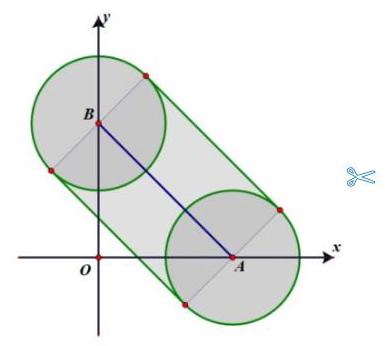
\includegraphics[max width=0.3\textwidth]{images/bo_d6dceus601uc73dvofhg_195_1027_1398_385_346_0.jpg}
\end{center}
\hspace*{3em} 

15.【2025.12 宝山高三一模 13】如果复平面上的向量 \(\overrightarrow{AB}\) 所对应的复数是 \(- 1 + {2i}\) ，则向量 \(\overrightarrow{BA}\) 所对应的复数是( )

A. \(1 - {2i}\) B. \(1 + {2i}\) C. \(- 1 + {2i}\) D. \(- 1 - {2i}\)

【答案】A※

16.【2025.12 崇明高三一模 14】已知 \(a,b \in  \mathbf{R}\) ，且 \(2 + a\mathrm{i}\) ， \(b + \mathrm{i}\) ( \(\mathrm{i}\) 是虚数单位)是实系数一元二次方程 \({x}^{2} + {px} + q = 0\) 的两个根,那么 \(p,q\) 的值分别是( )

A. \(p =  - 4,q = 5\) B. \(p =  - 4,q = 3\) C. \(p = 4,q = 5\) D. \(p = 4,q = 3\)

【答案】A

【解析】依题意可得: \(2 + {ai},b + i\) 互为共轭复数,故 \(a = 2,b =  - 1\) .

再由韦达定理得 \(\left\{  \begin{array}{l}  - p = \left( {2 + i}\right)  + \left( {2 - i}\right) \\  q = \left( {2 + i}\right) \left( {2 - i}\right)  \end{array}\right.\) ,计算得 \(\left\{  \begin{array}{l} p =  - 4 \\  q = 5 \end{array}\right.\) ,选 A. \(\lll\)

\section*{第十三章 数学建模}

\section*{13.1 三角模型}

1. 【2025.12 杨浦高三一模 11】某数学建模活动小组在开展主题为 “ 空中不可到达两点的测距问题 ” 的探究活动中,抽象并构建了如图所示的几何模型,该模型中 \({MA},{NB}\) 均与水平面 \({ABC}\) 垂直,在已测得可直接到达的两点间距离 \({AC},{BC}\) ,且 \({AC} < {BC}\) ,用测角仪测得 \(\angle {MCA},\angle {NCB}\) 的情况下,四名同学用测角仪各自测得下面一个角:  \circled{1}  \(\angle {ABC}\) ;  \circled{2} 

\(\angle {ACB}\) ； \circled{3}  \(\angle {BAC}\) ；(4) \(\angle {MCN}\) ，

其中一定能唯一确定 \(M\) ， \(N\) 之间的距离有\_\_\_\_\_. (写出所有正确的序号)

\begin{center}
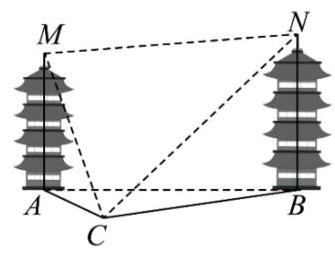
\includegraphics[max width=0.2\textwidth]{images/bo_d6dceus601uc73dvofhg_197_1065_767_335_253_0.jpg}
\end{center}
\hspace*{3em} 

【答案】 \circled{2}  \circled{3}  \circled{4} 

【解析】 \circled{1} 若测出 \(\angle {ABC}\) 的大小，则结合 \({AC},{BC}\) 的长度以及 \({AC} < {BC}\) ，在解 \(\bigtriangleup {ABC}\) 的过程中，会有 2 解，不唯一.

 \circled{2} 若测出 \(\angle {ACB}\) 的大小，则在 \(\bigtriangleup  {ABC}\) 中，由余弦定理求出 \({AB}\) 的长度.

已知 \(\angle {MCA},\angle {NCB}\) 的大小和 \({AC},{BC}\) 的长度,可计算出 \({AM},{BN}\) 的长度.

最后在直角梯形 \({AMNB}\) 中,根据 \({AB},{AM},{BN}\) 即可算出 \({MN}\) 的长度,且该值唯一.

 \circled{3} 若测出 \(\angle {BAC}\) 的大小，结合 \({AC},{BC}\) 的长度以及 \({AC} < {BC}\) ，可解出 \(\bigtriangleup {ABC}\) 的其余量，如 \({AB}\) 的长度. 接下来同条件 \circled{2} ，根据 \({AB},{AM},{BN}\) 即可算出 \({MN}\) 的长度，且该值唯一.

 \circled{4} 若测出 \(\angle {MCN}\) ，则首先可算出 \({MC},{NC}\) 的长度，进而在 \(\bigtriangleup  {MCN}\) 中，由余弦定理可求出 \({MN}\) 的长度,且该值唯一

2.【 2025.12 长宁高三一模 11】如图，两塔的塔尖分别为 \(M\) ， \(N\) ，塔底分别为 \(A\) ， \(B\) ，塔身 \({MA}\) ， \({NB}\) 均垂直水平面 \({ABC}\) . 已测得 \(C\) 与 \(A,B\) 的距离,4 名同学分别测得如下 4 组数据:

 \circled{1}  \(\angle {MCA},\angle {NCB},\angle {ACB}\) ；  \circled{2}  \(\angle {MCA},\angle {ACB},\angle {MCN}\) ；

 \circled{3}  \(\angle {MCA},\angle {NCB},\angle {MCN}\) ；  \circled{4}  \(\angle {MCA},\angle {ACB},\angle {NCA}\) .

其中不能唯一确定 \(M,N\) 之间距离的数据的序号有\_\_\_\_\_.

\begin{center}
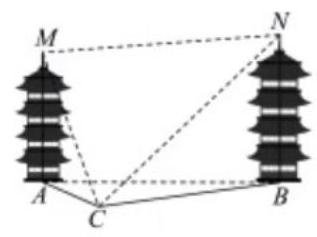
\includegraphics[max width=0.2\textwidth]{images/bo_d6dceus601uc73dvofhg_198_1026_214_317_237_0.jpg}
\end{center}
\hspace*{3em} 

【答案】 \circled{2}  \circled{4} 

【解析】 \circled{1} 若测出 \(\angle {ACB}\) 的大小,则在 \(\bigtriangleup {ABC}\) 中,由余弦定理求出 \({AB}\) 的长度.

已知 \(\angle {MCA},\angle {NCB}\) 的大小和 \({AC},{BC}\) 的长度,可计算出 \({AM},{BN}\) 的长度.

最后在直角梯形 \({AMNB}\) 中,根据 \({AB},{AM},{BN}\) 的长度即可算出 \({MN}\) 的长度,且该值唯一;

 \circled{2}  若测出 \(\angle {ACB}\) 的大小，则在 \(\bigtriangleup  {ABC}\) 中，由余弦定理求出 \({AB}\) 的长度.

再测出 \(\angle {MCA}\) 的大小和已知 \({AC}\) 的长度，可计算出 \({MC}\) 的长度.

此时再结合 \(\angle {MCN}\) 的大小，并不能唯一确定 \({MN}\) 的长度；

 \circled{3} 若测出 \(\angle {MCA},\angle {NCB}\) 的大小和 \({AC},{BC}\) 的长度,可计算出 \({CM},{CN}\) 的长度.

再测出 \(\angle {MCN}\) ,则在 \(\bigtriangleup {MCN}\) 中,由余弦定理可求出 \({MN}\) 的长度,且该值唯一.

 \circled{4} 若测出 \(\angle {NCA},\angle {ACB}\) 的大小,当 \(\angle {NCA} = \angle {ACB} = {90}^{ \circ  }\) 时,则 \(\angle {NCB}\) 的大小可为任意角, 此时 \({MN}\) 的长度也不唯一.

【总结】本题与 2026 届杨浦一模 11 题几乎一模一样.

3.【2025.12 黄浦高三一模 11】如图, 在一块空地上有四棵树, 若把它们所在的位置看成点,则这四个点 \(A,B,C,D\) 恰好是一个平行四边形的四个顶点,且 \({AB} = {40}\) 米, \({BC} = {30}\) 米, \(\angle {BAD} = {60}^{ \circ  }\) ,现要用挡板围出一个形状为矩形的展览区 \({EFGH}\) ,使得其边 \({EF},{FG},{GH},{HE}\) 分别经过点 \(A,B,C,D\) ，则该展览区的最大面积约为\_\_\_\_\_平方米(精确到 1 平方米) .

\begin{center}
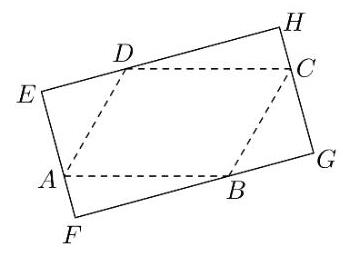
\includegraphics[max width=0.2\textwidth]{images/bo_d6dceus601uc73dvofhg_198_1057_1459_343_253_0.jpg}
\end{center}
\hspace*{3em} 

【答案】2136

【解析】依题意可设 \(\angle {ABF} = \theta\) (其中 \({0}^{ \circ  } \leq  \theta  \leq  {60}^{ \circ  }\) ),

\(\therefore {BF} = {40}\cos \theta ,{BG} = {30}\cos \left( {{60}^{ \circ  } - \theta }\right) ,{AF} = {40}\sin \theta ,{AE} = {30}\cos \left( {\theta  + {30}^{ \circ  }}\right)\) .

\(\therefore S = {FG} \cdot  {FE} = \left\lbrack  {{40}\cos \theta  + {30}\cos \left( {{60}^{ \circ  } - \theta }\right) }\right\rbrack   \cdot  \left\lbrack  {{40}\sin \theta  + {30}\cos \left( {\theta  + {30}^{ \circ  }}\right) }\right\rbrack\)

\(= \left\lbrack  {{15}\sqrt{3}\sin \theta  + {55}\cos \theta }\right\rbrack   \cdot  \left\lbrack  {{25}\sin \theta  + {15}\sqrt{3}\cos \theta }\right\rbrack   = {25}\left( {{15}\sqrt{3}{\sin }^{2}\theta  + {33}\sqrt{3}{\cos }^{2}\theta  + {82}\sin \theta \cos \theta }\right)\)

\(= {25}\left( {{41}\sin {2\theta } + 9\sqrt{3}\cos {2\theta } + {24}\sqrt{3}}\right)  = {25}\left\lbrack  {2\sqrt{481}\sin \left( {{2\theta } + \varphi }\right)  + {24}\sqrt{3}}\right\rbrack   \leq  {25}\left( {2\sqrt{481} + {24}\sqrt{3}}\right)  \approx  {2136}\)

该展览区的最大面积约为 2136 平方米.

4.【2025.12 徐汇高三一模 11】某城市核心区域可看作一个平面,市中心为点 \(O\) ,城市有两个交通枢纽站点 \(A,B\) ，其中站点 \(A\) 在市中心 \(O\) 的正东方向，距离 \(O\) 点 4 公里，站点 \(B\) 在市中心 \(O\) 的正北方向，距离 \(O\) 点也是 4 公里. 为了动态调整交通信号，相关部门计划在距离中心 \(O\) 点 2 公里的位置，设置一个移动数据采集点 \(C\) ，通过监测 \(\angle {ACB}\) 的大小来优化信号. 当 \(\angle {ACB}\) 最大时， \(\sin \angle {ACB} =\) \_\_\_\_\_. (结果精确到 0.01 )

【答案】0.54

【解析】依题意可得: \(A\left( {4,0}\right) ,B\left( {0,4}\right)\)

设 \(C\left( {2\cos \theta ,2\sin \theta }\right)\) ,则 \(\theta  \in  \left\lbrack  {0,\frac{\pi }{2}}\right\rbrack  ,\therefore \left\{  \begin{array}{l} {k}_{AC} = \frac{2\sin \theta }{2\cos \theta  - 4} \\  {k}_{BC} = \frac{2\sin \theta  - 4}{2\cos \theta } \end{array}\right.\) ,

\(\therefore \tan \angle {ACB} =  - \frac{\left| \begin{matrix} {k}_{AC} - {k}_{BC} \\  {k}_{AC} \end{matrix}\right| }{\left| 1 + {k}_{AC} \cdot  {k}_{BC}\right| } =  - \left| \frac{\frac{2\sin \theta }{2\cos \theta  - 4} - \frac{2\sin \theta  - 4}{2\cos \theta }}{1 + \frac{2\sin \theta }{2\cos \theta  - 4} \cdot  \frac{2\sin \theta  - 4}{2\cos \theta }}\right|  =  - \left| \frac{2\left( {\sin \theta  + \cos \theta }\right)  - 4}{1 - 2\left( {\sin \theta  + \cos \theta }\right) }\right|\) .

设 \(\sin \theta  + \cos \theta  = t \in  \left\lbrack  {1,\sqrt{2}}\right\rbrack\) ,则 \(\tan \angle {ACB} =  - \left| \frac{{2t} - 4}{1 - {2t}}\right|  =  - \frac{4 - {2t}}{{2t} - 1} = 1 - \frac{3}{{2t} - 1}\) .

所以 \({2t} - 1 \in  \left\lbrack  {1,2\sqrt{2} - 1}\right\rbrack\) ,当 \({2t} - 1 = 2\sqrt{2} - 1\) 时, \({\left( \tan \angle {ACB}\right) }_{\max } = \frac{2\sqrt{2} - 4}{2\sqrt{2} - 1}\) ,

此时 \(\sin \angle {ACB} = \frac{4 - 2\sqrt{2}}{\sqrt{{33} - {20}\sqrt{2}}} \approx  {0.54}\) .

5.【2025.12 金山高三一模 11】上海护珠塔, 俗称斜塔, 始建于北宋元丰年间 (1078\textasciitilde 1085 年), 是世界上倾斜程度最大的佛塔之一, 其倾斜角 (塔身所在直线与铅垂线的夹角) 超过意大利比萨斜塔. 如图,护珠塔前有一条笔直的山路,山路所在直线与水平面夹角为 \({34}^{ \circ  }\) . 康同学为了测量护珠塔的倾斜程度,实施如下方案: 从塔底 \(A\) 沿着山路往下走至 \(B\) ,此时测得 \({AB}\) 长度为 10 米,观察塔顶 \(D\) 的仰角 (视线与水平面的夹角) 为 \({76}^{ \circ  }\) ,继续往下走至 \(C\) , 测得 \({AC}\) 长度为 25.9 米,观察塔顶 \(D\) 的仰角为 \({60}^{ \circ  }\) . 根据康同学的数据,可得该塔的倾斜角为\_\_\_\_\_. (精确到 0.1 \textdegree )

\begin{center}
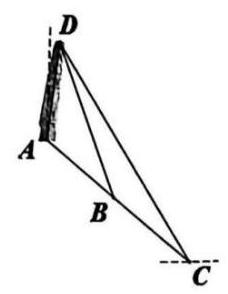
\includegraphics[max width=0.2\textwidth]{images/bo_d6dceus601uc73dvofhg_200_661_292_228_294_0.jpg}
\end{center}
\hspace*{3em} 

\begin{center}
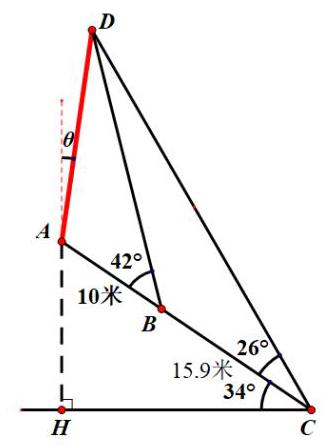
\includegraphics[max width=0.2\textwidth]{images/bo_d6dceus601uc73dvofhg_200_1066_211_324_446_0.jpg}
\end{center}
\hspace*{3em} 

【答案】 \({6.5}^{ \circ  }\)

【解析】作 \({AH} \bot\) 过点 \(C\) 的水平线,相关尺寸均已标出,如下图所示:

在 \(\bigtriangleup {BCD}\) 中, \(\angle {BDC} = {18}^{ \circ  }\) ,由正弦定理 \(\frac{BC}{\sin \angle {BDC}} = \frac{BD}{\sin \angle {BCD}}\) ,

代入可算出 \({BD} \approx  {25.287}\) .

在 \(\bigtriangleup  {BCD}\) 中，先由余弦定理 \(A{D}^{2} = A{B}^{2} + B{D}^{2} - {2AB} \cdot  {BD}\cos \angle {ABD}\) ，

代入算出 \({AD} \approx  {19.068}\) ；

再由正弦定理 \(\frac{AD}{\sin \angle {ABD}} = \frac{BD}{\sin \angle {BAD}}\) ,代入可算出 \(\angle {BAD} \approx  {117.457}^{ \circ  }\) .

而 \(\angle {CAH} = {90}^{ \circ  } - {34}^{ \circ  } = {56}^{ \circ  },\therefore \theta  = {180}^{ \circ  } - \angle {BAD} - \angle {CAH} \approx  {6.5}^{ \circ  }\) .

6.【2025.12 闵行高三一模 11】草坪上有一个带有围栏的边长为 \({30}\mathrm{\;m}\) 的正三角形活动区域 \({ABC}\) ,点 \(P\) 在边 \({BC}\) 上,且 \(\left| {PB}\right|  = 2\left| {PC}\right|\) ,小闵同学在该区域玩耍,他在 \(P\) 处放置了一个手电筒,若手电筒发出的光线张角 (任两条光线的最大夹角) 为 \({60}^{ \circ  }\) ,则手电筒在 \({ABC}\) 内部所能照射到的地面的最大面积为\_\_\_\_\_ \({\mathrm{m}}^{2}\) .

【答案】 \({125}\sqrt{3}\)

【解析】如图所示: 设光线与 \({AB},{AC}\) 边分别交于 \(E,F\) .

设 \(\angle {BPE} = \theta\) ,则 \(\theta  \leq  \arctan 3\sqrt{3}\) .

在 \(\bigtriangleup {BPE}\) 中,由正弦定理得 \(\frac{BP}{\sin \left( {{120}^{ \circ  } - \theta }\right) } = \frac{PE}{\sin {60}^{ \circ  }}\) ,

\(\therefore {PE} = \frac{{10}\sqrt{3}}{\sin \left( {{120}^{ \circ  } - \theta }\right) }\) . 所以 \({S}_{\bigtriangleup {BPE}} = \frac{1}{2}{BP} \cdot  {PE}\sin \theta  = \frac{{100}\sqrt{3}\sin \theta }{\sin \left( {{120}^{ \circ  } - \theta }\right) }\) ,

同理 \({S}_{\Delta CPF} = \frac{{25}\sqrt{3}\sin \left( {{120}^{ \circ  } - \theta }\right) }{\sin \theta } \cdot  {S}_{\Delta BPE} + {S}_{\Delta CPF} = \frac{{100}\sqrt{3}\sin \theta }{\sin \left( {{120}^{ \circ  } - \theta }\right) } + \frac{{25}\sqrt{3}\sin \left( {{120}^{ \circ  } - \theta }\right) }{\sin \theta }\) .

设 \(t = \frac{\sin \left( {{120}^{ \circ  } - \theta }\right) }{\sin \theta } = \frac{1}{2} \cdot  \frac{\sqrt{3}\cos \theta  + \sin \theta }{\sin \theta } = \frac{1}{2}\left( {1 + \sqrt{3}\cot \theta }\right)  \geq  \frac{2}{3}\) ,

则 \({S}_{\bigtriangleup {BPE}} + {S}_{\bigtriangleup {CPF}} = \frac{{100}\sqrt{3}}{t} + {25}\sqrt{3}t = {25}\sqrt{3}\left( {t + \frac{4}{t}}\right)  \geq  {25}\sqrt{3} \cdot  4 = {100}\sqrt{3}\) ,

当且仅当 \(t = \frac{4}{t}\) ,即 \(t = 2\) 时,也即 \(\theta  = {30}^{ \circ  }\) 时,等号成立,

此时阴影部分面积最大为 \(S = {225}\sqrt{3} - {100}\sqrt{3} = {125}\sqrt{3}{\mathrm{\;m}}^{2}\) .

\begin{center}
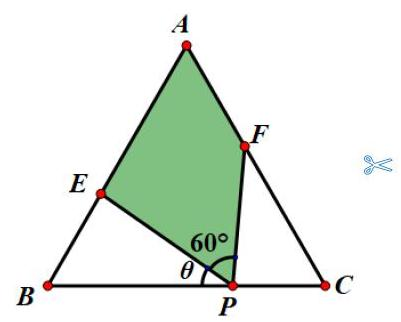
\includegraphics[max width=0.3\textwidth]{images/bo_d6dceus601uc73dvofhg_201_1010_579_401_322_0.jpg}
\end{center}
\hspace*{3em} 

7.【2025.12 奉贤高三一模 12】运动员关心的是在足球场上的哪些位置射门命中的角度较大. 在真实的射门过程中, 我们做一些假定:

(1)将足球看成一个质点;

(2)接近球门时, 足球运动的轨迹与地面平行;

(3)射门时，足球与球门之间无防守员;

(4)足球场平面图是一个矩形;

(5)标准足球场的长度为 105 米，宽度为 68 米，球门的宽度为 7.32 米；

如图,以线段 \({AB}\) 所在直线为 \(y\) 轴,以线段 \({AB}\) 的垂直平分线为 \(x\) 轴建立平面直角坐标系, \(O\) 是球门中心,两门柱位置分别为点 \(A\text{ 、 }B\) ,两个角球点为 \(C\text{ 、 }D,{EF}\) 是半场分界线.

对于区域 \({CDEF}\) 内,射门点 \(P\left( {x,y}\right)\) ,

对于每一个确定的横坐标 \(x\) ,可以找到唯一的 \(y\) ,可以证明横坐标不变时, \(y = 0\) 时, \(\angle {APB}\) 最大. 此时,点 \(P\) 在 \(x\) 轴上是最佳射门点.

对于每一个确定的纵坐标 \(y\left( {{3.66} < y < {34}}\right)\) ,同样可以找到唯一的 \(x\) ,当 \(x =\) \_\_\_\_\_时, \(\angle {APB}\) 最大. 此时,点 \(P\) 是最佳射门点.

\begin{center}
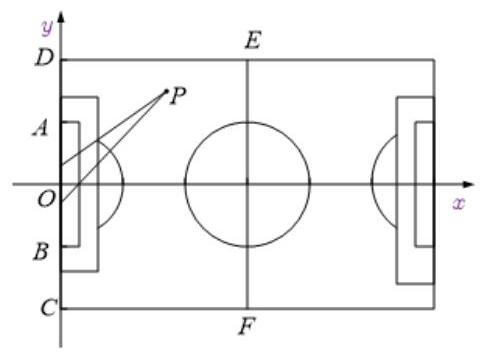
\includegraphics[max width=0.4\textwidth]{images/bo_d6dceus601uc73dvofhg_202_912_195_480_354_0.jpg}
\end{center}
\hspace*{3em} 

【答案】 \(\sqrt{{y}^{2} - {3.66}^{2}}\)

【解析】如图建系,若 \(y\) 给定,以 \({AB}\) 为弦画圆,则圆心 \(M\) 在 \(x\) 轴上, \(\therefore {MP} \bot  x\) 轴, 此时 \({MP} = {MA} = {MB}\) ,即 \({x}^{2} + {3.66}^{2} = {y}^{2}\) ,即 \(x = \sqrt{{y}^{2} - {3.66}^{2}}\) 时,张角 \(\angle {APB}\) 最大. \(\propto\)

8.【2025.12 青浦高三一模 16】如图所示,水平地面上插有两根杆子 \({AB}\) 和 \({CD},{AB}\) 所在直线垂直于地面且 \({AB} = 2\) 米， \({CD}\) 所在直线与地面斜交. 小明有一把卷尺. 他在某时刻分别测出杆子 \({AB}\) 和 \({CD}\) 在阳光下影子的长度,称为一次操作. 小明可以在白天除正午外的不同时刻进行多次操作. 假设阳光为平行光,正午时分 \({AB}\) 的影子长度为 0 . 则下列说法正确的是 ( ).

A. 为求出 \({CD}\) 的长度,小明至少需要进行 2 次操作

B. 为求出 \({CD}\) 的长度,小明至少需要进行 3 次操作

C. 为求出 \({CD}\) 的长度,小明至少需要进行 4 次操作

D. 无论进行多少次操作,小明都不能求出 \({CD}\) 的长度

\begin{center}
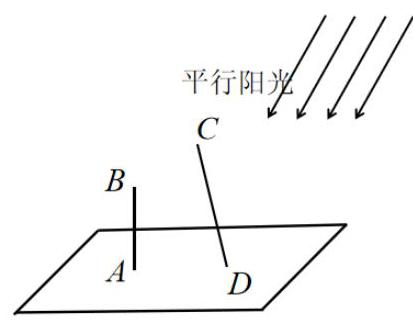
\includegraphics[max width=0.3\textwidth]{images/bo_d6dceus601uc73dvofhg_202_322_1370_413_323_0.jpg}
\end{center}
\hspace*{3em} 

\begin{center}
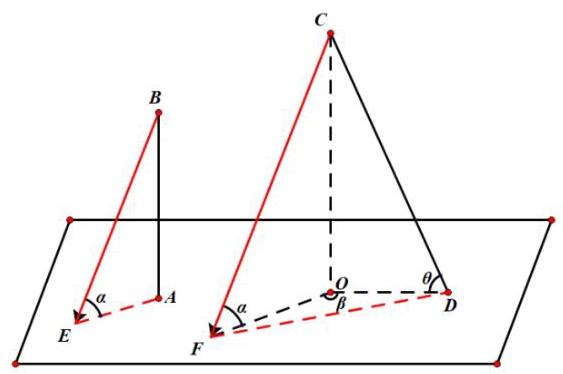
\includegraphics[max width=0.4\textwidth]{images/bo_d6dceus601uc73dvofhg_202_839_1331_563_374_0.jpg}
\end{center}
\hspace*{3em} 

【答案】B

【解析】 \circled{1} 设 \({CD}\) 与底面的夹角为 \(\theta\) ,则 \({CO} = {CD}\sin \theta ,{DO} = {CD}\cos \theta\) ;

 \circled{2} 在某个时刻，测出杆子 \({AB}\) 和 \({CD}\) 在阳光下影子的长度 \({AE}\) 和 \({DF}\) 的长度；

 \circled{3} 设此时阳光与底面的夹角为 \(\alpha\) ,则 \(\tan \alpha  = \frac{AB}{AE} = \frac{CO}{FO}\) ,

从而得 \({CF} = \frac{CO}{\sin \alpha },{FO} = \frac{{CD}\sin \theta  \cdot  {AE}}{AB}\) ;

 \circled{4} 设 \(\angle {DOF} = \beta\) ,在 \({\Delta DOF}\) 中,由余弦定理得 \(D{F}^{2} = O{D}^{2} + O{F}^{2} - {2OD} \cdot  {OF}\cos \beta\) ;

 \circled{5}  整理化简: \(D{F}^{2} = {\left( CD\cos \theta \right) }^{2} + {\left( \frac{{CD}\sin \theta  \cdot  {AE}}{AB}\right) }^{2} - {2CD}\cos \theta  \cdot  \frac{{CD}\sin \theta  \cdot  {AE}}{AB} \cdot  \cos \beta\) .

在上述等式中, \({AB},{AE},{DF}\) 均为已知量, \({CD},\theta ,\beta\) 均为待求的未知量,

故需要测量三次, 从而可得 3 个方程, 联立方程组即可解出 3 个变量, 故选 B.C.<

9.【2025.12 嘉定高三一模 21】图 1 为转角过道的地面平面示意图. 该过道由两条直道连接形成转角, 由水平平坦的地面与垂直于地面的墙面共同围成, 两端延伸至足够远处, 且高度充足.其中, \({QA}\text{ 、 }{QB}\) 构成地面上过道的一侧边界, \(\angle {AQB} = {120}^{ \circ  }\) ; 地面上过道的另一侧边界,则分别与 \({QA}\text{ 、 }{QB}\) 平行,且交于点 \(P\) .过道两侧平行墙面之间的距离均为 3 米.

(1)如图 2，在地面有一圆，该圆与 \({QA}\text{ 、 }{QB}\) 均相切，且过点 \(P\) . 求此圆的半径:

(2)如图 3，有一根长度为 \(y\) 米的无粗细木棒 \({MN}\) 紧贴地面，端点 \(N\) 沿 \({QB}\) 移动，另一端点 \(M\) 沿 \({AQ}\) 移动. 当木棒 \({MN}\) 触碰到点 \(P\) 时， \(\angle {QMN} = x\) (弧度)，求 \(y\) 关于 \(x\) 的函数关系及 \(y\) 的最小值;

(3)如图4，某长方体家具的底面为长方形 \({EFGH}\) ，其宽为 1 米，长为 10 米(因过道高度足够， 无需考虑家具高度).现将底面 EFGH 紧贴地面移动，判断该家具能否顺利通过此转角过道，并说明理由.

【答案】(1) \(\left( {{12} - 6\sqrt{3}}\right)\)

(2) \(y = \frac{3}{\sin x} + \frac{3}{\sin \left( {{60}^{ \circ  } - x}\right) },{y}_{\min } = {12}\) (3)否

【解析】(1) 设该圆半径为 \(r\) ,圆心为 \(O\) ,则 \(O\) 在 \({PQ}\) 上,且 \(O\) 到 \({QA}\) 的距离为 \(r\) ,

因此 \({OQ} = \frac{2r}{\sqrt{3}}\) . (1 分)

\({PQ} = \frac{6}{\sqrt{3}} = r + \frac{2}{\sqrt{3}}r\) . 解得 \(r = \frac{2\sqrt{3}}{1 + \frac{2}{\sqrt{3}}} = {12} - 6\sqrt{3}\) (米) . 此圆的半径为 \(\left( {{12} - 6\sqrt{3}}\right)\) 米.

(2)如图，作 \({PC} \bot  {QM}\) 于 \(C\) ，作 \({PD} \bot  {QN}\) 于 \(D\) ，

则 \(\left| {MN}\right|  = \left| {MP}\right|  + \left| {PN}\right|  = \frac{\left| PC\right| }{\sin \angle {QMP}} + \frac{\left| PD\right| }{\sin \angle {QNP}} = \frac{3}{\sin x} + \frac{3}{\sin \left( {\frac{\pi }{3} - x}\right) }\)

因此, \(y = f\left( x\right)  = \frac{3}{\sin x} + \frac{3}{\sin \left( {\frac{\pi }{3} - x}\right) }\left( {0 < x < \frac{\pi }{3}}\right)\) .

\({f}^{\prime }\left( x\right)  =  - \frac{3\cos x}{{\sin }^{2}x} + \frac{3\cos \left( {\frac{\pi }{3} - x}\right) }{{\sin }^{2}\left( {\frac{\pi }{3} - x}\right) } = \frac{3\cos \left( {\frac{\pi }{3} - x}\right) {\sin }^{2}x - 3\cos x{\sin }^{2}\left( {\frac{\pi }{3} - x}\right) }{{\sin }^{2}x{\sin }^{2}\left( {\frac{\pi }{3} - x}\right) }.\)

当 \(x \in  \left( {0,\frac{\pi }{6}}\right\rbrack\) 时, \(\cos x \geq  \cos \left( {\frac{\pi }{3} - x}\right)  > 0,\sin \left( {\frac{\pi }{3} - x}\right)  \geq  \sin x > 0\) ,

因此, \(3\cos \left( {\frac{\pi }{3} - x}\right) {\sin }^{2}x \leq  3\cos x{\sin }^{2}\left( {\frac{\pi }{3} - x}\right)\) ,所以 \({f}^{\prime }\left( x\right)  \leq  0\) ,等号仅当 \(x = \frac{\pi }{6}\) 取到,

所以 \(y = f\left( x\right)\) 在 \(\left( {0,\frac{\pi }{6}}\right\rbrack\) 内严格减. 因为 \(y = f\left( x\right)\) 的图像关于 \(x = \frac{\pi }{6}\) 对称,

所以 \({f}_{\min }\left( x\right)  = f\left( \frac{\pi }{6}\right)  = {12}\) . 即在 \(x = \frac{\pi }{6}\) 时, \(y\) 取到最小值 12 (米).

\begin{center}
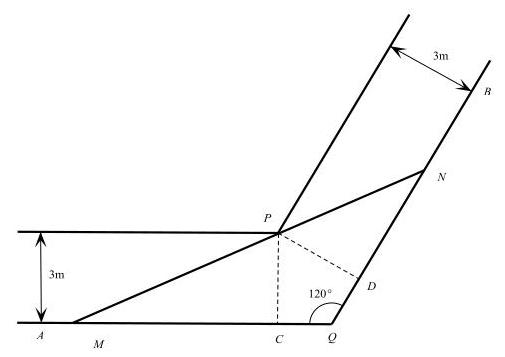
\includegraphics[max width=0.4\textwidth]{images/bo_d6dceus601uc73dvofhg_204_394_1273_505_357_0.jpg}
\end{center}
\hspace*{3em} 

\begin{center}
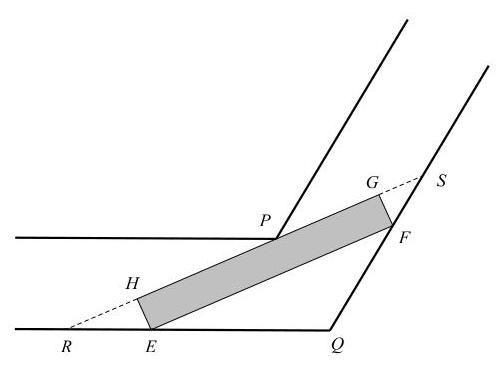
\includegraphics[max width=0.4\textwidth]{images/bo_d6dceus601uc73dvofhg_204_905_1268_500_365_0.jpg}
\end{center}
\hspace*{3em} 

(3)设底面长方形的顶点 \(E\) 、 \(F\) 分别在边界 \({AQ}\) 、 \({QB}\) 上移动，设 \(\angle {QEF} = \alpha\) . 假设长方体的边 \({GH}\) 过 \(P\) 点，如图，延长 \({HG}\) 交 \({QA}\) 于 \(R\) ，交 \({QB}\) 于 \(S\) ， 则 \(\left| {RS}\right|  = \left| {RH}\right|  + \left| {HG}\right|  + \left| {GS}\right|  = \frac{1}{\tan \alpha } + \left| {HG}\right|  + \frac{1}{\tan \left( {\frac{\pi }{3} - \alpha }\right) }\) . 由 \(\left| {RS}\right|  = \frac{3}{\sin \alpha } + \frac{3}{\sin \left( {\frac{\pi }{3} - \alpha }\right) }\) ,因此 \(\left| {HG}\right|  = \frac{3}{\sin \alpha } + \frac{3}{\sin \left( {\frac{\pi }{3} - \alpha }\right) } - \frac{1}{\tan \alpha } - \frac{1}{\tan \left( {\frac{\pi }{3} - \alpha }\right) }\) . 记 \(g\left( \alpha \right)  = \frac{3}{\sin \alpha } + \frac{3}{\sin \left( {\frac{\pi }{3} - \alpha }\right) } - \frac{1}{\tan \alpha } - \frac{1}{\tan \left( {\frac{\pi }{3} - \alpha }\right) }\) ,则 \(g\left( \alpha \right)\) 表示在 \(\angle {QEF} = \alpha\) 时家具边 \({GH}\) 恰好通过点 \(P\) 时的长度(家具能通过的最大允许长度). 长为 10 米的家具能顺利通过转角过道的必要条件是:对任意的 \(\alpha  \in  \left( {0,\frac{\pi }{3}}\right)\) ， \(g\left( \alpha \right)  \geq  {10}\) .

然而, \(g\left( \frac{\pi }{6}\right)  \approx  {8.53} < {10}\) . 因此上述必要条件不成立. 故,该家具不能通过该转角过道. \(\gg   <\)

\section*{13.2 函数模型}

1. 【2025.12 松江高三一模 11】某社区为扩大居民的活动区域，计划将社区内原有的半径为 \({10}\mathrm{\;m}\) 的圆形花坛扩建成一个矩形花园. 若要求扩建前的圆与扩建后矩形的两邻边和一条对角线都相切，则矩形花园占地面积的最小值为\_\_\_\_\_(结果精确到 \(1{\mathrm{\;m}}^{2}\) ).

【答案】1166

【解析】如图所示: 圆 \(M\) 为 \({Rt\Delta ABC}\) 的内切圆,设 \({AB} = a,{AD} = b\) ,

则 \({DG} = {DE} = a - {10},{BG} = {BF} = b - {10}\) ,从而可得 \({BD} = {DG} + {BG} = a + b - {20}\) .

由勾股定理得 \(A{B}^{2} + A{D}^{2} = B{D}^{2}\) ,代入计算得 \({ab} + {200} = {20}\left( {a + b}\right)  \geq  {40}\sqrt{ab}\) ,解得

\(\sqrt{ab} \geq  {20} + {10}\sqrt{2}\left( {\sqrt{ab} \leq  {20} - {10}\sqrt{2}\text{ 舍 }}\right)\) ,所以 \({ab} \geq  {100}\left( {6 + 4\sqrt{2}}\right)  \approx  {1166}\) .

故矩形花园占地面积的最小值为 1166 平方米.

\begin{center}
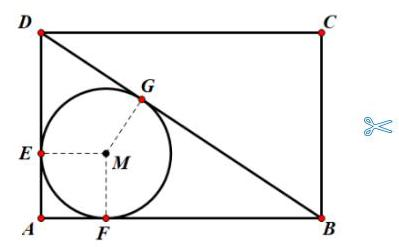
\includegraphics[max width=0.3\textwidth]{images/bo_d6dceus601uc73dvofhg_205_1010_1210_399_247_0.jpg}
\end{center}
\hspace*{3em} 

2.【2025.12 虹口高三一模 10】小虹同学要在边长为 10 的正方形纸片 RSNM 上剪出一个等腰梯形 \({ABCD}\) 的图案，如图所示，腰 \({AB},{CD}\) 与正方形内的抛物线 \(\Gamma\) 分别相切于 \(E,F\) 两点， 其中 \(\Gamma\) 的顶点 \(O\) 为 \({RM}\) 的中点. 若当点 \(E\) 到 \({RM}\) 的距离为 4.5 时, \({EF} = 6\) ,则当等腰梯形 \({ABCD}\) 的面积取到最小值时， \({EF} =\) \_\_\_\_\_(结果保留 2 位小数).

\begin{center}
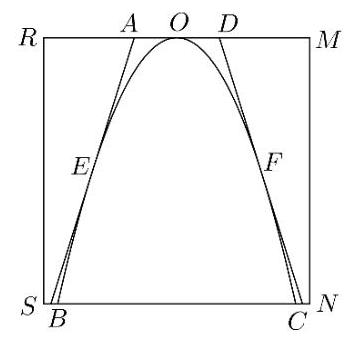
\includegraphics[max width=0.2\textwidth]{images/bo_d6dceus601uc73dvofhg_205_1049_1740_348_337_0.jpg}
\end{center}
\hspace*{3em} 

【答案】6.32

【解析】设抛物线的解析式为 \(f\left( x\right)  = a{x}^{2}\) (其中 \(a < 0\) ),将 \(E\left( {-3, - \frac{9}{2}}\right)\) 代入得 \(a =  - \frac{1}{2}\) .

设 \(E\left( {{x}_{0}, - \frac{1}{2}{x}_{0}^{2}}\right)\) ,可得 \({k}_{AB} = {f}^{\prime }\left( {x}_{0}\right)  =  - {x}_{0}\) ,故直线 \({AB}\) 的方程为 \(y - \left( {-\frac{1}{2}{x}_{0}^{2}}\right)  =  - {x}_{0}\left( {x - {x}_{0}}\right)\) ,

即从而可得 \(A\left( {\frac{{x}_{0}}{2},0}\right) ,B\left( {\frac{{x}_{0}}{2} + \frac{10}{{x}_{0}}, - {10}}\right)\) . 再根据对称性可知 \({AD} = {x}_{0},{BC} = {x}_{0} + \frac{20}{{x}_{0}}\) .

所以等腰梯形 \({ABCD}\) 的面积为

\(S = \frac{1}{2}\left( {{AD} + {BC}}\right) h = \frac{1}{2}\left( {2{x}_{0} + \frac{20}{{x}_{0}}}\right)  \cdot  {10} = {10}\left( {{x}_{0} + \frac{10}{{x}_{0}}}\right)  \geq  {20}\sqrt{10},\)

当且仅当 \({x}_{0} =  - \sqrt{10}\) 时,等号成立,此时 \({x}_{F} = \sqrt{10},\therefore {EF} = 2\sqrt{10} \approx  {6.32}\) 。

3.【2025.12 宝山高三一模 19】如图,摩天轮上一点 \(P\) 距离地面的高度 \(y\left( m\right)\) 关于时间 \(t\left( \min \right)\) 的函数表达式为: \(y = A\sin \left( {{\omega t} + \varphi }\right)  + b,\left( {A > 0,\omega  > 0,\left| \varphi \right|  \leq  \pi }\right)\) . 已知摩天轮的半径为 \({30}\mathrm{\;m}\) ,其中心点 \(O\) 距地面 \({40}\mathrm{\;m}\) ,摩天轮以每 12 分钟转一圈的方式做匀速转动,而点 \(P\) 的超始位置在摩天轮的最低点处.

(1)根据条件具体写出 \(y\) 关于 \(t\) 的函数表达式;

(2)在摩天轮转动的一圈内，点 \(P\) 有多长时间距离地面超过 \({55}\mathrm{m}\) ?

\begin{center}
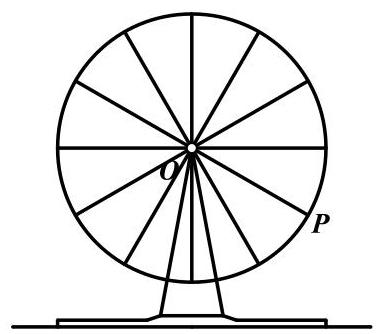
\includegraphics[max width=0.3\textwidth]{images/bo_d6dceus601uc73dvofhg_206_1019_1286_379_334_0.jpg}
\end{center}
\hspace*{3em} 

【答案】(1) \(y = {30}\sin \left( {\frac{\pi }{6}t - \frac{\pi }{2}}\right)  + {40} =  - {30}\cos \frac{\pi }{6}t + {40}\)

(2) \({30}\sin \left( {\frac{\pi }{6}x - \frac{\pi }{2}}\right)  + {40} \geq  {55}\) ，有 4 分钟

【解析】(1) 摩天轮的半径为 \({30m}\) ,则 \(A = {30}\) ,中心点 \(O\) 距地面 \({40m}\) ,则 \(b = {40}\) 每 12 分钟转一圈,则 \(T = {12}\) ,即 \(\frac{2\pi }{\omega } = {12}\) ,解得 \(\omega  = \frac{\pi }{6}\) ,所以 \(y = {30}\sin \left( {\frac{\pi }{6}t + \phi }\right)  + {40}\) 点 \(P\) 的起始位置在摩天轮的最低点处,则 \(t = 0\) 时, \(y = {30}\sin \phi  + {40} = {10}\) , 此时 \(\sin \phi  =  - 1\) ,又 \(\left| \phi \right|  \leq  \pi\) ,所以 \(\phi  =  - \frac{\pi }{2}\) 所以 \(y\left( m\right)\) 关于 \(t\left( \min \right)\) 的函数表达式为 \(y = {30}\sin \left( {\frac{\pi }{6}t - \frac{\pi }{2}}\right)  + {40} =  - {30}\cos \frac{\pi }{6}t + {40}\)

(2)由题意得 \(y =  - {30}\cos \frac{\pi }{6}t + {40} > {55}\) 即 \(\cos \frac{\pi }{6}t <  - \frac{1}{2}\)

其中 \(t \in  \left\lbrack  {0,{12}}\right\rbrack\) ,则 \(\frac{\pi }{6}t \in  \left\lbrack  {0,{2\pi }}\right\rbrack\) ,从而 \(\frac{\pi }{6}t \in  \left( {\frac{2}{3}\pi ,\frac{4}{3}\pi }\right)\) 所以 \(t \in  \left( {4,8}\right)\)

所以在摩天轮转动的一圈内,点 \(P\) 有 4 分钟时间距离地面超过 \({55m}\) .
\end{document}